% !TeX program = latexmk
\documentclass[paper=b5j,fontsize=11Q,jafontsize=11Q,baselineskip=19Q]{jlreq}

\RequirePackage[twoside,inner=21mm,outer=27mm,top=25mm,bottom=23mm,
  headheight=14pt,headsep=7mm,footskip=10mm]{geometry}
\RequirePackage{luatexja}
\RequirePackage{luatexja-fontspec}
\RequirePackage{mathtools,amssymb,bm}
\RequirePackage{tikz}
\usetikzlibrary{arrows.meta,calc,decorations.markings,positioning,angles,quotes}
\RequirePackage{booktabs,tabularx,array}
\RequirePackage{enumitem}
\RequirePackage{etoolbox}
\RequirePackage{fancyhdr}
\RequirePackage{xcolor}
\RequirePackage[most]{tcolorbox}
\RequirePackage{hyperref}
\RequirePackage{bookmark}
\RequirePackage{needspace}

\definecolor{HiroBlue}{gray}{0.15}
\definecolor{HiroBlueLight}{gray}{0.94}
\definecolor{WarmGray}{gray}{0.97}
\definecolor{WarmGrayDark}{gray}{0.38}
\definecolor{DeepInk}{gray}{0}
\definecolor{AnswerGreen}{gray}{0.48}

\tcbset{
  solutionmajor/.style={
    enhanced,breakable,
    colback=HiroBlueLight,colframe=HiroBlue,
    boxrule=.55pt,arc=1mm,
    left=7pt,right=7pt,top=6pt,bottom=6pt,
    before skip=0pt,after skip=.55\baselineskip
  },
  solutionminor/.style={
    enhanced,breakable,
    colback=white,colframe=WarmGrayDark,
    boxrule=.4pt,arc=.8mm,
    left=6pt,right=6pt,top=5pt,bottom=5pt,
    before skip=.8\baselineskip,after skip=.55\baselineskip
  }
}

\hypersetup{
  colorlinks=true,
  linkcolor=black,
  urlcolor=black,
  citecolor=black,
  pdfborder={0 0 0}
}

\setlength{\parindent}{1em}
\setlength{\parskip}{0pt}
\setlength{\abovedisplayskip}{8pt plus 2pt minus 2pt}
\setlength{\belowdisplayskip}{8pt plus 2pt minus 2pt}
\setlength{\abovedisplayshortskip}{5pt plus 2pt}
\setlength{\belowdisplayshortskip}{5pt plus 2pt}
\setlist{itemsep=.25\baselineskip,topsep=.35\baselineskip,leftmargin=2em}

\newcommand{\runningtitle}{章題未定}
\pagestyle{fancy}
\fancyhf{}
\fancyhead[LE]{\sffamily\small 篠澤広に超弦理論を教えてもらう本}
\fancyhead[RO]{\sffamily\small \runningtitle}
\fancyfoot[LE,RO]{\sffamily\small\thepage}
\renewcommand{\headrulewidth}{0.35pt}
\renewcommand{\footrulewidth}{0pt}

\newcommand{\alphap}{\alpha'}
\newcommand{\Z}{\mathbb{Z}}
\newcommand{\R}{\mathbb{R}}
\newcommand{\dd}{\mathrm{d}}
\newcommand{\e}{\mathrm{e}}
\newcommand{\imunit}{\mathrm{i}}
\newcommand{\term}[1]{\textbf{#1}}
\newcommand{\cl}{\mathrm{cl}}
\newcommand{\spherearea}{\Omega_{n-1}}

\newcommand{\stepmark}[1]{%
  {\sffamily\bfseries #1.}%
}
\renewcommand{\theHsection}{\arabic{part}.\arabic{section}}
\renewcommand{\theHsubsection}{\theHsection.\arabic{subsection}}
\renewcommand{\theHsubsubsection}{\theHsubsection.\arabic{subsubsection}}
\numberwithin{equation}{section}
\newcommand{\recordbreak}[1]{%
  \par\addvspace{.8\baselineskip}%
  \needspace{3\baselineskip}%
  \noindent{\sffamily\bfseries #1}\par
  \nobreak\smallskip
}
\newcounter{exercise}[section]
\renewcommand{\theexercise}{\Roman{part}-\arabic{section}-\arabic{exercise}}
\newcommand{\problemformulas}[1]{%
  \par\addvspace{.45\baselineskip}%
  {\color{WarmGrayDark}\hrule height .4pt}%
  \begingroup
  \setlength{\abovedisplayskip}{6pt}%
  \setlength{\belowdisplayskip}{6pt}%
  #1%
  \endgroup
  {\color{WarmGrayDark}\hrule height .4pt}%
  \par\addvspace{.45\baselineskip}%
}
\newcommand{\answerheading}[1]{%
  \par\addvspace{.9\baselineskip}%
  \needspace{4\baselineskip}%
  \noindent{\sffamily\bfseries #1}\par
  \nobreak\smallskip
}
\newif\ifloweranswers
\newif\ifanswerconclusionused
\newcommand{\answerconclusion}[1]{%
  \global\answerconclusionusedtrue
  \par\nobreak\smallskip
  \noindent\ensuremath{\therefore}\quad #1\par
}
\newenvironment{storybox}[1][]{%
  \par\addvspace{.6\baselineskip}%
  \if\relax\detokenize{#1}\relax\else\recordbreak{#1}\fi
}{\par\addvspace{.5\baselineskip}}
\newenvironment{boardbox}[1]{\recordbreak{#1}}{\par\addvspace{.5\baselineskip}}
\newenvironment{checkpointbox}[1]{\recordbreak{#1}}{\par\addvspace{.5\baselineskip}}
\newenvironment{definitionbox}[1]{\recordbreak{#1}}{\par\addvspace{.5\baselineskip}}
\newenvironment{exercisebox}[1]{\recordbreak{#1}}{\par\addvspace{.7\baselineskip}}
\newif\ifsolutionafterheading
\newcommand{\prepareanswerheading}{%
  \ifsolutionafterheading\else\clearpage\fi
  \global\solutionafterheadingtrue
}
\pretocmd{\section}{\prepareanswerheading}{}{}
\pretocmd{\subsection}{\prepareanswerheading}{}{}
\newif\ifsolutionstatementopen
\newcommand{\closesolutionstatement}{%
  \ifsolutionstatementopen
    \end{tcolorbox}%
    \solutionstatementopenfalse
  \fi
}
\newcommand{\solutionpart}[4]{%
  \global\answerconclusionusedfalse
  \closesolutionstatement
  \par\addvspace{.35\baselineskip}%
  \Needspace{7\baselineskip}%
  \begin{tcolorbox}[solutionminor]
    \noindent{\sffamily\bfseries
      \if\relax\detokenize{#1}\relax 問題\else (#1)\fi}\quad
    #2
  \end{tcolorbox}
  \answerheading{考え方}
  #3\par
  \answerheading{解いてみる}
  #4\par
  \nobreak\smallskip
  \noindent\hfill
  \ensuremath{\square}\par
}
% 本文の列挙後に置かれた追加設問も、同じ形式で独立して再掲する。
\newcommand{\solutionfollowup}[3]{\solutionpart{まとめ}{#1}{#2}{#3}}
\newcommand{\solutionprelude}[1]{%
  \par\addvspace{.45\baselineskip}%
  #1\par
}
\newenvironment{solutionbox}[1]{%
  \ifsolutionafterheading
    \global\solutionafterheadingfalse
  \else
    \clearpage
  \fi
  \refstepcounter{exercise}%
  \begingroup
  \solutionstatementopentrue
  \begin{tcolorbox}[solutionmajor]
  \noindent{\sffamily\bfseries 第\arabic{exercise}問\quad #1%
    \hfill\normalfont\small（\theexercise）}\par
  \smallskip
  \ignorespaces
}{%
  \closesolutionstatement
  \par
  \endgroup
  \par\addvspace{.8\baselineskip}%
}
\begin{document}
\renewcommand{\runningtitle}{別冊解答}
\hypersetup{pageanchor=false}
\begin{titlepage}
  \thispagestyle{empty}
  \vspace*{26mm}
  \begin{center}
    {\sffamily\bfseries\fontsize{18pt}{24pt}\selectfont
      篠澤広に\\[2mm]超弦理論を教えてもらう本\par}
    \vspace{8mm}
    \rule{.72\linewidth}{1pt}\\[5mm]
    {\sffamily\bfseries\fontsize{12pt}{17pt}\selectfont
      別冊解答\par}
    \vfill
    {\sffamily warm snow\par}
    \vspace{3mm}
    {\sffamily\small 2026年12月29日\par}
  \end{center}
\end{titlepage}

\hypersetup{pageanchor=true}
\pagenumbering{roman}
\setcounter{tocdepth}{2}
\tableofcontents
\clearpage
\pagenumbering{arabic}

\begin{checkpointbox}{この別冊について}
補習で宿題を出した次の日、広は二人の答案を返すとき、自分の解き方を書いた紙を一緒に渡した。
この別冊は、その紙を章ごとに並べたものだ。
解き方の文は、広が千奈と佑芽に宛てて書いたままにしてある。

大問ごとに頁を変えて、最初の枠に問題と、共通の条件を書いた。
小問は問題文を省かずにもう一度書き、そのあとに「考え方」と「解いてみる」を置いた。

先に「考え方」だけを読んで、使う式を一つ手元に書いてみるとよい。
そこで止まったら、「解いてみる」の同じところを読む。何を代入して、どの条件を使ったかが、行ごとに書いてある。
計算の問題は、最後の数字に加えて、符号と単位と、成り立つ条件まで比べる。
証明や考察の問題は、出発点の仮定から結論まで、つながっているかを見る。
小問の終わりの$\square$は、そこでその小問が終わる印。

難しさの順は「確認」「誘導付き」「本気」。
「追加」は条件を変える問題、「比較」は二つを並べる問題、
「考察」は意味と限界を言葉にする問題、「総合」は節や章をまたぐ問題。
「予告」と「発展」は先を少しのぞく問題で、解かなくても先へ進める。
\end{checkpointbox}

\begin{definitionbox}{記号で迷ったときに}
$c=\hbar=1$の自然単位では、長さと時間は、質量の逆数の単位になる。
「質量次元$[A]=d$」は、$A$の単位が質量の$d$乗、という意味。$[A]=M^d$と書いても同じ。
たとえば半径は$[R]=-1$、弦の定数は$[\alpha']=-2$。だから$\alpha'M^2$は無次元。

$=$は、定義か、置いた仮定のもとで成り立つ等式。
$\simeq$は、捨てた項と、近似が使える条件を書いた近似。
$\sim$は、極限でいちばん大きい項や、order-oneの係数を省いた依存のしかた。どちらの意味かは、その小問の条件と一緒に読む。
$O(x^n)$は、$x\to0$で$x^n$の定数倍以下に収まる、省いた項のまとめ。

式を移す前に、2乗がふつうの数の2乗か、計量を使った内積かを確かめる。
この本のMinkowski計量では$p^2=-(p^0)^2+|\boldsymbol p|^2$なので、
2乗と書いてあっても、正とは限らない。
\end{definitionbox}

\begin{definitionbox}{略称を先に確認する}
略して書いたものを、先に並べておく。
\begin{description}[leftmargin=3.3em,labelsep=.8em,style=nextline]
  \item[KK] Kaluza--Klein。円にした余剰次元の運動量が、低次元では質量の塔に見える。
  \item[BRST] Becchi--Rouet--Stora--Tyutin。ゲージ同値性を保った共変量子化の整合性を検査する。
  \item[NS/R] Neveu--Schwarz/Ramond。世界面フェルミオンの反周期境界条件と周期境界条件を表す。
  \item[GSO] Gliozzi--Scherk--Olive射影。量子論の整合性と時空超対称性に合う状態を選ぶ。
  \item[CFT/OPE] 共形場理論と演算子積展開。相互作用と相関関数まで含む世界面理論を記述する。
  \item[RR/BPS] Ramond--Ramond電荷とBogomolny--Prasad--Sommerfield状態。
    後者は超対称代数が与える質量または張力の下限を飽和する。
  \item[DBI] Dirac--Born--Infeld作用。Dブレーンの幾何と世界体積ゲージ場を一つにまとめる。
  \item[AdS/CFT] anti-de Sitter時空と共形場理論の対応。
    RTはRyu--Takayanagi公式、QESは量子極値面を表す。
  \item[EFT/WGC] 有効場の理論と弱重力予想。後者は量子重力における電荷と重力の強さを制約する予想。
\end{description}
\end{definitionbox}

\clearpage
\part[課題解答　第1章〜第7章]{課題解答\\第1章〜第7章}
\setcounter{section}{0}
\begingroup
\renewcommand{\runningtitle}{解答 第1章　次元と物理量}
\newcommand{\dimof}[1]{\left[#1\right]}
\newcommand{\Mdim}{\mathsf{M}}
\newcommand{\Ldim}{\mathsf{L}}
\newcommand{\Tdim}{\mathsf{T}}
\newcommand{\GN}{G_{\mathrm N}}
\newcommand{\lP}{\ell_{\mathrm P}}
\newcommand{\tP}{t_{\mathrm P}}
\thispagestyle{empty}
\section[次元と物理量　課題解答]{次元と物理量──課題解答}
\subsection{数字の前に、何を測るか──解答}

プランク長さを作った日の終わりに、広は4問の宿題を出した。
集めた二人の答えを返すとき、広は1問ずつ解き方を書いた紙を添えた。

\begin{solutionbox}{確認　単位換算}
\solutionpart{}{%
\problemformulas{%
\begin{align*}
72\,\frac{\mathrm{km}}{\mathrm{h}}
  &\times
  \frac{1000\,\mathrm{m}}{1\,\mathrm{km}}
  \times
  \frac{1\,\mathrm{h}}{3600\,\mathrm{s}}
  \\
  &=
  20\,\frac{\mathrm{m}}{\mathrm{s}}.
  \tag{A}
\end{align*}
}
自動車の速さ $90\,\mathrm{km\,h^{-1}}$ を
$\mathrm{m\,s^{-1}}$ へ換算する。
式\textup{(A)}と同じように、掛けた二つの換算係数と、
消えた単位も書くこと。
}{変えたいのは単位だけで、速さの値は変えない。
だから、値が1の換算係数 $1000\,\mathrm{m}/(1\,\mathrm{km})$ と $1\,\mathrm{h}/(3600\,\mathrm{s})$ を掛ける。
置く向きは、消したい $\mathrm{km}$ と $\mathrm{h}$ が、分子と分母で向かい合うように。
約分して $\mathrm{m\,s^{-1}}$ だけが残れば、向きは合ってる。}{%
式\textup{(A)}の $72$ を $90$ に替えて、同じ二つの換算係数を掛ける。
$\mathrm{km}$ は換算係数の分母に、$\mathrm{h}$ は分子に置く。
\begin{align}
  90\,\frac{\mathrm{km}}{\mathrm{h}}
  &\times
  \frac{1000\,\mathrm{m}}{1\,\mathrm{km}}
  \times
  \frac{1\,\mathrm{h}}{3600\,\mathrm{s}}
  \notag\\
  &=
  \frac{90\times1000}{3600}\,
  \frac{\mathrm{m}}{\mathrm{s}}
  \notag\\
  &=
  25\,\mathrm{m\,s^{-1}}.
  \label{eq:answer-speed}
\end{align}
掛けた換算係数は $1000\,\mathrm{m}/(1\,\mathrm{km})$ と $1\,\mathrm{h}/(3600\,\mathrm{s})$。
どっちも値は1だから、速さそのものは変わってない。
消えた単位は $\mathrm{km}$ と $\mathrm{h}$ で、分子と分母で約分されて、$\mathrm{m\,s^{-1}}$ だけが残った。
}
\end{solutionbox}

\begin{solutionbox}{確認　足せる項を確かめる}
\solutionpart{}{%
\problemformulas{%
\begin{equation*}
v=v_0+at
  \tag{A}
\end{equation*}

\begin{equation*}
x=x_0+v_0t+\frac12at^2
  \tag{B}
\end{equation*}
}
式\textup{(A)}と
\textup{(B)}から導いた式
\begin{equation}
  v^2=v_0^2+2a(x-x_0)
\end{equation}
について、左辺と右辺の各項の次元を $\Ldim,\Tdim$ で表し、
足し算が可能なことを確かめる。
次に
\begin{equation}
  v^2=v_0^2+2at
\end{equation}
が次元的に成立しない理由を書く。
}{足せるのは、次元が同じものどうしだけ。
$\dimof{v}=\Ldim\Tdim^{-1}$ と $\dimof{a}=\Ldim\Tdim^{-2}$ を使って、二つの式の項を一つずつ、基本の次元に戻して比べる。
二つ目の式では、ほかと次元がそろわない項がどれかを探す。}{%
速度と加速度の次元は
\begin{equation}
  \dimof{v}=\Ldim\Tdim^{-1},
  \qquad
  \dimof{a}=\Ldim\Tdim^{-2}.
\end{equation}
左辺は
\begin{equation}
  \dimof{v^2}
  =
  \Ldim^2\Tdim^{-2}.
\end{equation}
右辺の第1項も
\begin{equation}
  \dimof{v_0^2}
  =
  \Ldim^2\Tdim^{-2}.
\end{equation}
第2項では、$x-x_0$ が長さの次元を持つので
\begin{align}
  \dimof{a(x-x_0)}
  &=
  (\Ldim\Tdim^{-2})\Ldim
  \notag\\
  &=
  \Ldim^2\Tdim^{-2}.
\end{align}
係数の2は、次元のない数。
三つの項が同じ次元 $\Ldim^2\Tdim^{-2}$ になったから、
\begin{equation}
  v^2=v_0^2+2a(x-x_0)
\end{equation}
は、足し算も等号も、次元の上では成り立つ。

二つ目の式の第2項は
\begin{equation}
  \dimof{at}
  =
  (\Ldim\Tdim^{-2})\Tdim
  =
  \Ldim\Tdim^{-1}.
\end{equation}
これは速度の次元で、速度の2乗の $\Ldim^2\Tdim^{-2}$ じゃない。
$2a(x-x_0)$ の、長さの $x-x_0$ を、時間の $t$ に替えた形になっていて、替えた分だけ次元がずれた。
だから
\begin{equation}
  v^2=v_0^2+2at
\end{equation}
は、第2項をほかの項に足せない。
次元のちがう項を足した式は、ある単位でたまたま数が合っても、単位を替えると成り立たなくなる。
秒を分に替えると、$v^2$ と $v_0^2$ の数値は3600倍、$at$ の数値は60倍になって、項ごとに倍率がそろわない。

佑芽の最初の式も、同じ種類の間違いだった。
$v_0$ のあとに $t$ が抜けていて、長さに速さを足してた。
}
\end{solutionbox}

\begin{solutionbox}{誘導付き　ばねの周期を再現する}
\solutionpart{}{%
ばねの力 $F=-kx$ と、そこから求めた
$\dimof{k}=\Mdim\Tdim^{-2}$ を使う。
周期を
\begin{equation}
  P_{\mathrm s}=C m^\alpha k^\beta
\end{equation}
と置き、質量と時間の指数を比較して
$P_{\mathrm s}=C\sqrt{\frac{m}{k}}$ を再現する。
最後に、次元解析だけでは $C=2\pi$ を決められない理由を書く。
}{周期が、質量 $m$ とばね定数 $k$ だけで決まると仮定して、$P_{\mathrm s}=C m^\alpha k^\beta$ と置く。
$\dimof{k}=\Mdim\Tdim^{-2}$ を使って、両辺の質量の指数と時間の指数をそろえる。
未知数は $\alpha,\beta$ の二つで、式も2本。
$C$ のほうは、次元を比べる式のどこに入るかを見ておく。}{%
ばねの力 $F=-kx$ から出した、ばね定数の次元は
\begin{equation}
  \dimof{k}=\Mdim\Tdim^{-2}.
\end{equation}
周期の候補
\begin{equation}
  P_{\mathrm s}=C m^\alpha k^\beta
\end{equation}
の右辺は
\begin{align}
  \dimof{m^\alpha k^\beta}
  &=
  \Mdim^\alpha
  (\Mdim\Tdim^{-2})^\beta
  \notag\\
  &=
  \Mdim^{\alpha+\beta}
  \Tdim^{-2\beta}.
\end{align}
左辺は周期だから $\Tdim$。
長さ $\Ldim$ は、両辺のどっちにも入ってない。
質量と時間の指数を比べる。
\begin{equation}
  \alpha+\beta=0,
  \qquad
  -2\beta=1.
\end{equation}
第2式から $\beta=-1/2$。
第1式に入れて $\alpha=1/2$。
だから
\begin{equation}
  P_{\mathrm s}
  =
  C m^{1/2}k^{-1/2}
  =
  C\sqrt{\frac{m}{k}}.
  \label{eq:answer-spring}
\end{equation}

$C$ は次元のない数。
指数を比べた2本の式に、$C$ は一度も出てこない。
$C=2\pi$ でも $C=2$ でも、右辺の次元は同じ $\Tdim$ になる。
だから、次元解析だけでは $C=2\pi$ を選べない。
五円玉の振り子でも、測った $6.3$ から言えたのは、$2\pi$ に近い、まで。
係数まで決めるには、おもりが一瞬ごとにどう動くかを式にして、解く。
そのための道具は微分で、道具ができたら、このばねで確かめる。
}
\end{solutionbox}

\begin{solutionbox}{本気　プランク時間を作る}
\solutionpart{}{%
\problemformulas{%
\begin{equation*}
\dimof{c}=\Ldim\Tdim^{-1}.
  \tag{A}
\end{equation*}

\begin{equation*}
\dimof{\hbar}
  =
  \frac{\dimof{E}}{\dimof{\omega}}
  =
  \Mdim\Ldim^2\Tdim^{-1}.
  \tag{B}
\end{equation*}

\begin{align*}
\dimof{\GN}
  &=
  \frac{\dimof{F}\dimof{r}^2}
  {\dimof{m_1}\dimof{m_2}}
  \\
  &=
  \frac{
  (\Mdim\Ldim\Tdim^{-2})\Ldim^2
  }{\Mdim^2}
  \\
  &=
  \Ldim^3\Mdim^{-1}\Tdim^{-2}.
  \tag{C}
\end{align*}
}
式\textup{(A)}、\textup{(B)}、
\textup{(C)}で求めた三定数の次元を使う。
時間 $\tP$ を
\begin{equation}
  \tP=Cc^\alpha\hbar^\beta\GN^\gamma
\end{equation}
と置き、指数 $\alpha,\beta,\gamma$ を求める。
$C=1$ とした結果が
\begin{equation}
  \tP=\sqrt{\frac{\hbar\GN}{c^5}}
\end{equation}
になること、さらに $\tP=\frac{\lP}{c}$ と一致することを確かめる。
}{プランク長さと同じ材料から、今度は時間を作る。
$\tP=Cc^\alpha\hbar^\beta\GN^\gamma$ と置いて、右辺の質量・長さ・時間の指数を、左辺の $\Tdim$ とそろえる。
式は3本で、未知数も $\alpha,\beta,\gamma$ の三つ。
長さのときと違うのは、そろえる先が $\Mdim^0\Ldim^0\Tdim^1$ になるところだけ。
解く順番は、長さのときに千奈が見つけたやり方で決める。
$\gamma=\beta$ だけを言う1本目を先に入れて、次に右辺が0の式を使う。
出てきた式は、$\lP/c$ と比べて検算する。}{%
三つの定数の次元は
\begin{equation}
  \dimof{c}=\Ldim\Tdim^{-1},
  \qquad
  \dimof{\hbar}=\Mdim\Ldim^2\Tdim^{-1},
  \qquad
  \dimof{\GN}=\Ldim^3\Mdim^{-1}\Tdim^{-2}.
\end{equation}
候補
\begin{equation}
  \tP=Cc^\alpha\hbar^\beta\GN^\gamma
\end{equation}
の右辺をまとめると
\begin{equation}
  \Mdim^{\beta-\gamma}
  \Ldim^{\alpha+2\beta+3\gamma}
  \Tdim^{-\alpha-\beta-2\gamma}.
\end{equation}
ここまでは、プランク長さのときとまったく同じ。
作りたいのは時間だから、右辺を $\Mdim^0\Ldim^0\Tdim^1$ にそろえる。
指数を比べて
\begin{align}
  \beta-\gamma&=0,\\
  \alpha+2\beta+3\gamma&=0,\\
  -\alpha-\beta-2\gamma&=1.
  \label{eq:answer-planck-time-system}
\end{align}

1本目は $\gamma=\beta$ だけを言っているから、先にそれを使う。
右辺が0の2本目に入れると $\alpha+5\beta=0$ で、$\alpha=-5\beta$。
これで、3本目に残る文字は $\beta$ だけになる。
長さのときは、右辺が0なのが3本目だったから、千奈は3本目を先に使った。
今度は、それが2本目。
\begin{equation}
  5\beta-\beta-2\beta=1,
\end{equation}
だから
\begin{equation}
  \beta=\gamma=\frac12,
  \qquad
  \alpha=-\frac52.
\end{equation}
次元のない $C$ は、長さのときと同じで、決めようがない。
$C=1$ と約束すれば
\begin{equation}
  \tP
  =
  c^{-5/2}\hbar^{1/2}\GN^{1/2}
  =
  \sqrt{\frac{\hbar\GN}{c^5}}.
  \label{eq:answer-planck-time}
\end{equation}
長さのときの答えと比べると、$\beta=\gamma=\frac12$ は変わらず、$c$ の指数だけが $-\frac32$ から $-\frac52$ に動いた。

検算として、プランク長さを光速で割ってみる。
\begin{align}
  \frac{\lP}{c}
  &=
  \frac1c
  \sqrt{\frac{\hbar\GN}{c^3}}
  \notag\\
  &=
  \sqrt{\frac{\hbar\GN}{c^5}}
  =
  \tP.
\end{align}
長さを速さで割ったから、次元は時間。
指数を解いて出した式と、$\lP/c$ から作った式が、同じ式になった。
}
\end{solutionbox}

\subsubsection*{解答を閉じる前に}

4問の中でいちばん取り違えやすいのは、4問目の $c$ の指数。
$\sqrt{\hbar\GN/c^3}$ と $\sqrt{\hbar\GN/c^5}$ は、$c$ が二つ違うだけで、長さと時間に分かれる。
覚えた形をたよりに書くと、どっちを書いたか、自分では見分けられない。
根号の中を $\Mdim,\Ldim,\Tdim$ に戻して、$\Ldim^2$ になれば長さ、$\Tdim^2$ になれば時間。

1問目と3問目の答えも、単位を戻せば確かめられる。
$25\,\mathrm{m\,s^{-1}}$ は $\mathrm{km}$ と $\mathrm{h}$ が消えた残りで、$\sqrt{m/k}$ の単位は $\sqrt{\mathrm{kg}/(\mathrm{kg\,s^{-2}})}=\mathrm{s}$。
単位で確かめられないのは、次元のない数だけ。
4問目の $C$ は、どの組み合わせをプランク時間と呼ぶかの約束だから、1にしてよかった。
ばねの周期は測れる量で、$C$ を勝手に選ぶと、測った周期とずれる。
3問目の $C$ は、運動を解いて出す。
\clearpage
\endgroup
\begingroup
\renewcommand{\runningtitle}{解答 第2章　微積分・テンソル・作用}
\newcommand{\pder}[2]{\frac{\partial #1}{\partial #2}}
\renewcommand{\runningtitle}{解答 第2章　微積分・テンソル・作用}
\section[微積分・テンソル・作用　課題解答]{微積分・テンソル・作用──課題解答}
\subsection[変化を数える]{変化を数える--微分、積分、変分──解答}


\begin{solutionbox}{確認　微分・偏微分・全微分}
$f(x,y)=x^2y+\sin y$とする。
\solutionpart{1}{%
$y$を固定して、偏微分
\[
  \frac{\partial f}{\partial x}
\]
を求めよ。
}{偏微分 $\frac{\partial f}{\partial x}$ は、$y$ を止めて $x$ だけ動かしたときの変化率。
止めた $y$ は、ただの数として扱える。項ごとに、$x$ が入っているかを見る。}{%
$y$は止めるから、ただの数として扱う。$f$を二つの項に分けて、一つずつ$x$で微分する。
\begin{align*}
  \pder{}{x}\bigl(x^2y\bigr)&=y\,\pder{}{x}\bigl(x^2\bigr)=y\cdot2x=2xy,\\
  \pder{}{x}\bigl(\sin y\bigr)&=0 .
\end{align*}
二つ目は、$x$が入ってないから、$x$を動かしても変わらない。だから$0$。
足すと
\begin{equation}
  {\pder{f}{x}=2xy}.
\end{equation}
確かめ。$y=1$に止めると$f=x^2+\sin1$で、ふつうの微分は$2x$。式に$y=1$を入れても$2x\cdot1=2x$。合ってる。
}
\solutionpart{2}{%
$x$を固定して、偏微分
\[
  \frac{\partial f}{\partial y}
\]
を求めよ。
}{今度は $x$ を止めて、$y$ だけ動かす。偏微分 $\frac{\partial f}{\partial y}$ はその変化率。
$x^2y$ の $x^2$ は係数。$\sin y$ には $\frac{\dd(\sin y)}{\dd y}=\cos y$ を使う。}{%
今度は$x$を止める。$x^2$はただの係数。
\begin{align*}
  \pder{}{y}\bigl(x^2y\bigr)&=x^2\,\pder{}{y}(y)=x^2\cdot1=x^2,\\
  \pder{}{y}\bigl(\sin y\bigr)&=\cos y .
\end{align*}
足すと
\begin{equation}
  {\pder{f}{y}=x^2+\cos y}.
\end{equation}
設問(1)と比べると、同じ$x^2y$でも、どっちを止めるかで係数の役が入れ替わる。$x$で微分したら$y$が係数、$y$で微分したら$x^2$が係数。
}
\solutionpart{3}{%
全微分$\dd f$を書け。
}{全微分は $\dd f=(\frac{\partial f}{\partial x})\dd x+(\frac{\partial f}{\partial y})\dd y$。
$x$ と $y$ を少しずつ動かしたときの、1次の変化を足したもの。
係数には、設問(1)の $\frac{\partial f}{\partial x}$ と設問(2)の $\frac{\partial f}{\partial y}$ をそのまま入れればいい。}{%
全微分は、$x$と$y$を同時に少しずつ動かしたときの、$f$の1次の変化。
\begin{equation*}
  f(x+\dd x,\,y+\dd y)-f(x,y)
  =\pder{f}{x}\dd x+\pder{f}{y}\dd y+(\text{2次以上}).
\end{equation*}
1次の部分を$\dd f$と書く。
\begin{equation*}
  \dd f=\pder{f}{x}\dd x+\pder{f}{y}\dd y.
\end{equation*}
設問(1)の$\pder fx=2xy$と、設問(2)の$\pder fy=x^2+\cos y$を入れると
\begin{equation}
  {\dd f=2xy\dd x+(x^2+\cos y)\dd y}.
\end{equation}
小さく動かして、数で比べる。$(x,y)=(1,0)$から$\dd x=0.01$、$\dd y=0$だけ動かすと、式は$2\cdot1\cdot0\cdot0.01=0$。実際$f(1.01,0)-f(1,0)=0-0=0$。$\dd y=0.01$なら式は$(1+1)\cdot0.01=0.02$で、実際は$1\cdot0.01+\sin0.01\simeq0.02$。
}
\solutionpart{4}{%
$x(t)=t^2$、$y(t)=t$に沿う全微分
\[
  \frac{\dd f}{\dd t}
\]
をchain ruleで求め、
    $f(t^2,t)$を直接微分した結果と一致することを確かめよ。
}{曲線 $x(t),y(t)$ に沿って微分するなら、chain rule $\frac{\dd f}{\dd t}=(\frac{\partial f}{\partial x})\dot x+(\frac{\partial f}{\partial y})\dot y$。
$f$ の時間変化を、$x$ を通る分と $y$ を通る分に分けて足す。
検算には、先に $x,y$ を入れてしまった $f(t^2,t)$ を使う。}{%
$x=t^2$、$y=t$なので$\dot x=2t$、$\dot y=1$。chain ruleから
\begin{align}
  \frac{\dd f}{\dd t}
  &=2xy\dot x+(x^2+\cos y)\dot y\notag\\
  &=2(t^2)(t)(2t)+(t^4+\cos t)\notag\\
  &={5t^4+\cos t}.
\end{align}
検算。$f(t^2,t)=t^5+\sin t$ を直接微分しても、同じ $5t^4+\cos t$ になる。
}
\end{solutionbox}

\begin{solutionbox}{確認　部分積分と境界項}
2回微分可能な関数$x(t)$について、
\solutionpart{1}{%
積の微分
\[
  \frac{\dd}{\dd t}(x\dot x)
\]
を展開せよ。
}{$x\dot x$ は、$t$ で動くものの積。だから積の微分 $\frac{\dd}{\dd t}(uv)=\dot u v+u\dot v$ を、$u=x$, $v=\dot x$ で使う。
こうしておくと、次の設問で積分する $x\ddot x$ が、全微分と $\dot x^2$ に分かれる。}{%
積の微分を、$u=x$、$v=\dot x$で使う。
\begin{equation*}
  \frac{\dd}{\dd t}(uv)=\dot u\,v+u\,\dot v .
\end{equation*}
$\dot u=\dot x$、$\dot v=\ddot x$だから
\begin{align}
  \frac{\dd}{\dd t}(x\dot x)
  &=\dot x\cdot\dot x+x\cdot\ddot x\notag\\
  &={\dot x^2+x\ddot x}.
\end{align}
$x=t^2$で試す。$x\dot x=t^2\cdot2t=2t^3$で、微分は$6t^2$。右は$\dot x^2+x\ddot x=(2t)^2+t^2\cdot2=4t^2+2t^2=6t^2$。両辺とも同じ。
この式の右の$x\ddot x$が、次の設問で部分積分したいもの。
}
\solutionpart{2}{%
設問(1)で得た
\[
  \frac{\dd}{\dd t}(x\dot x)=\dot x^2+x\ddot x
\]
を$t_i$から$t_f$まで積分し、
    \[
      \int_{t_i}^{t_f}x\ddot x\dd t
      =[x\dot x]_{t_i}^{t_f}
      -\int_{t_i}^{t_f}\dot x^2\dd t
    \]
    を示せ。
}{設問(1)の $\frac{\dd}{\dd t}(x\dot x)=\dot x^2+x\ddot x$ を、$t_i$ から $t_f$ まで積分する。
左辺は全微分だから、積分すると端の値 $[x\dot x]_{t_i}^{t_f}$ だけになる。補習で千奈が左辺を時刻の決まらない $uv$ と書いて、佑芽に「いつの$uv$？」と聞かれたのが、ここ。あとは $\int x\ddot x\,\dd t$ について解く。}{%
両辺を$t_i$から$t_f$まで積分すると
\[
  [x\dot x]_{t_i}^{t_f}
  =\int_{t_i}^{t_f}\dot x^2\dd t
   +\int_{t_i}^{t_f}x\ddot x\dd t.
\]
左辺は、両端の値の差。右辺の第2項について解けば
\begin{equation}
  {
  \int_{t_i}^{t_f}x\ddot x\dd t
  =[x\dot x]_{t_i}^{t_f}
  -\int_{t_i}^{t_f}\dot x^2\dd t}.
\end{equation}
}
\solutionpart{3}{%
$x(t_i)=x(t_f)=0$のとき境界項を評価せよ。
}{境界項を端の値で書くと $[x\dot x]_{t_i}^{t_f}=x(t_f)\dot x(t_f)-x(t_i)\dot x(t_i)$。
途中の時刻の値は入っていない。だから、両端の条件 $x(t_i)=x(t_f)=0$ だけで決まる。}{%
境界項を、両端の値に書き下す。
\begin{equation*}
  [x\dot x]_{t_i}^{t_f}
  =x(t_f)\dot x(t_f)-x(t_i)\dot x(t_i).
\end{equation*}
$x(t_i)=x(t_f)=0$を入れると、どっちの項にも$0$が掛かる。
\begin{equation}
  [x\dot x]_{t_i}^{t_f}
  =0\cdot\dot x(t_f)-0\cdot\dot x(t_i)={0}.
\end{equation}
$\dot x$の値は何でもいい。掛ける相手がゼロだから。
設問(2)の式は
\begin{equation*}
  \int_{t_i}^{t_f}x\ddot x\dd t=-\int_{t_i}^{t_f}\dot x^2\dd t
\end{equation*}
になる。境界項が消えると、部分積分は「微分を移して符号を変える」だけになる。
}
\solutionpart{4}{%
設問(2)で得た境界項
$[x\dot x]_{t_i}^{t_f}$は、
$x$でなく$\dot x$だけを端で固定しても消えるか。
理由とともに答えよ。
}{消したいのは $[x\dot x]_{t_i}^{t_f}$。$x$ と $\dot x$ の積。
$\dot x$ を固定したとき、積のもう片方の $x$ が、端でどうなっているかを見る。
「固定する」と「ゼロにする」は違う。そこを分けて考えて。}{%
端の項を、端ごとに書き出す。
\begin{equation*}
  [x\dot x]_{t_i}^{t_f}=x(t_f)\dot x(t_f)-x(t_i)\dot x(t_i).
\end{equation*}
端で$\dot x(t_i)=v_i$、$\dot x(t_f)=v_f$と固定すると
\begin{equation*}
  [x\dot x]_{t_i}^{t_f}=v_f\,x(t_f)-v_i\,x(t_i).
\end{equation*}
$x(t_i)$と$x(t_f)$は固定してないから、ゼロとは限らない。たとえば$x(t)=v t+1$、$t_i=0$、$t_f=1$なら
\begin{equation*}
  [x\dot x]_0^1=v(v+1)-v\cdot1=v^2\ne0\quad(v\ne0).
\end{equation*}
だから、ふつうは消えない。
消えるのは、たとえば$v_i=v_f=0$まで決めたとき。それは、固定する値をゼロに選んだ特別な場合で、「$\dot x$を固定した」より強い条件。
}
\end{solutionbox}

\begin{solutionbox}{誘導付き　離散作用}
\problemformulas{%
\begin{equation*}
S_N=\sum_{i=0}^{N-1}
  \left[
    \frac m2\left(\frac{q_{i+1}-q_i}{\Delta t}\right)^2
    -V(q_i)
  \right]\Delta t
  \tag{A}
\end{equation*}
}
式\textup{(A)}で$N=4$とし、端点$q_0,q_4$を固定する。
\solutionprelude{%
$N=4$では
\[
  S_4=\sum_{i=0}^{3}
  \left[\frac m2
  \left(\frac{q_{i+1}-q_i}{\Delta t}\right)^2
  -V(q_i)\right]\Delta t.
\]
}
\solutionpart{1}{%
$q_2$を含む項だけを書き出せ。
}{$q_2$ を動かして変わるのは、$q_2$ が入ってる項だけ。
運動の項 $(q_{i+1}-q_i)^2$ とpotentialの項 $V(q_i)$ で、どの $i$ に $q_2$ が入るかを別々に数える。
$q_2$ が入ってない項は、$q_2$ を動かしても変わらないから、省いていい。}{%
運動の項では$i=1,2$、potentialの項では$i=2$に、$q_2$が入る。
\begin{equation}
  S_4\big|_{q_2}
  =\frac{m}{2\Delta t}(q_2-q_1)^2
   +\frac{m}{2\Delta t}(q_3-q_2)^2
   -V(q_2)\Delta t.
\end{equation}
$q_2$が入っていない項は、省いた。
}
\solutionpart{2}{%
偏微分
\[
  \frac{\partial S_4}{\partial q_2}
\]
を求めよ。
}{$\frac{\partial S_4}{\partial q_2}$ では、$q_2$ が入ってない項は微分して0。
設問(1)で取り出した三つの項だけを $q_2$ で微分する。2乗の項が二つあって、片方は中身の $q_2$ に負号が付いている。}{%
設問(1)の三つの項を、一つずつ$q_2$で微分する。
一つ目は$(q_2-q_1)^2$の微分で、中身の$q_2$の係数は$+1$。
\begin{equation*}
  \pder{}{q_2}\left[\frac m{2\Delta t}(q_2-q_1)^2\right]
  =\frac m{2\Delta t}\cdot2(q_2-q_1)\cdot(+1)
  =\frac m{\Delta t}(q_2-q_1).
\end{equation*}
二つ目は$(q_3-q_2)^2$で、中身の$q_2$の係数は$-1$。だから、微分にも$-1$が掛かる。
\begin{equation*}
  \pder{}{q_2}\left[\frac m{2\Delta t}(q_3-q_2)^2\right]
  =\frac m{2\Delta t}\cdot2(q_3-q_2)\cdot(-1)
  =-\frac m{\Delta t}(q_3-q_2).
\end{equation*}
三つ目はpotential。
\begin{equation*}
  \pder{}{q_2}\bigl[-V(q_2)\Delta t\bigr]=-V'(q_2)\Delta t .
\end{equation*}
足してまとめると
\begin{align}
  \pder{S_4}{q_2}
  &=\frac{m}{\Delta t}(q_2-q_1)
   -\frac{m}{\Delta t}(q_3-q_2)
   -V'(q_2)\Delta t\notag\\
  &={
    \frac{m}{\Delta t}(2q_2-q_1-q_3)
    -V'(q_2)\Delta t}.
\end{align}
$2q_2-q_1-q_3$は、$q_2$が両隣の平均よりどれだけ上にいるか、の2倍。次の設問で、これが加速度になる。
}
\solutionpart{3}{%
停留条件から$q_2$における差分運動方程式を導け。
}{実際に通る道では、内側の点を少し動かしても、作用は1次では変わらない。だから、設問(2)の $\frac{\partial S_4}{\partial q_2}$ をゼロと置く。
目標の形は、$q_3-2q_2+q_1$ を $(\Delta t)^2$ で割ったもの。差分を2回取った形になる。}{%
$\frac{\partial S_4}{\partial q_2}=0$をまとめると
\begin{align}
  0
  &=\pder{S_4}{q_2}\notag\\
  &=\frac{m}{\Delta t}(q_2-q_1)
   -\frac{m}{\Delta t}(q_3-q_2)
   -V'(q_2)\Delta t\notag\\
  &=\frac{m}{\Delta t}(2q_2-q_1-q_3)
   -V'(q_2)\Delta t,\notag\\
  \frac{m}{\Delta t}(2q_2-q_1-q_3)
  &=V'(q_2)\Delta t,\notag\\
  \frac{m}{(\Delta t)^2}(2q_2-q_1-q_3)
  &=V'(q_2).\notag
\end{align}
両辺の符号を反転すると
\begin{equation}
  {
  m\frac{q_3-2q_2+q_1}{(\Delta t)^2}=-V'(q_2)}.
\end{equation}
}
\solutionpart{4}{%
$V=0$なら$q_{i+1}-q_i$が$i$によらず一定になることを示し、折れ線の形を説明せよ。
}{$V=0$ なら力 $-V'(q_i)$ は消える。差分の運動方程式は $q_{i+1}-2q_i+q_{i-1}=0$ だけになる。
これを、隣どうしの差が等しい、という形に並べ替える。時刻の間隔はどこも $\Delta t$ だから、差は折れ線の各区間の傾きと同じことを表す。}{%
$V=0$なら、内側のどの点でも
\[
  q_{i+1}-2q_i+q_{i-1}=0.
\]
したがって
\begin{equation}
  {q_{i+1}-q_i=q_i-q_{i-1}}.
\end{equation}
隣の点との高さの差が、どこでも同じ。時刻の間隔も$\Delta t$で同じだから、折れ線のどの区間も傾きが等しい。
だから点は、両端を結ぶ直線の上に、等間隔に並ぶ。力のない粒は、一定の速さで進む。
}
\end{solutionbox}

\begin{solutionbox}{誘導付き　一様重力中の粒子}
上向きを$z$の正方向とし
\[
  L(z,\dot z)=\frac m2\dot z^2-mgz
\]
とする。
\solutionpart{1}{%
二つの偏微分
\[
  \frac{\partial L}{\partial z},\qquad
  \frac{\partial L}{\partial\dot z}
\]
を求めよ。
}{Euler--Lagrange方程式に要るのは、$\frac{\partial L}{\partial z}$ と $\frac{\partial L}{\partial\dot z}$ の二つ。
$L=m\dot z^2/2-mgz$ のうち、位置が入ってるのはpotentialの項だけ、速度が入ってるのは運動の項だけ。それぞれ微分する。}{%
偏微分のときは、$L(z,\dot z)$の二つの引数を、別々のものとして扱う。
$z$で微分するときは$\dot z$を止めて、$\dot z$で微分するときは$z$を止める。だから
\begin{align*}
  \pder{L}{z}&=0-mg=-mg,\\
  \pder{L}{\dot z}&=\frac m2(2\dot z)-0=m\dot z.
\end{align*}
このあと、実際の運動$z(t)$に沿って時間で微分するときは、$\dot z$も$t$で動く。偏微分のときに止めるのと、時間で微分するときに動かすのは、別の操作。
}
\solutionpart{2}{%
Euler--Lagrange方程式から$\ddot z=-g$を導け。
}{Euler--Lagrange方程式 $\frac{\dd}{\dd t}\left(\frac{\partial L}{\partial\dot z}\right)-\frac{\partial L}{\partial z}=0$ は、作用が止まる条件を、$z$ の運動方程式にしたもの。
設問(1)の二つの偏微分を入れて、$m\ne0$ だから $\ddot z$ について解く。}{%
Euler--Lagrange方程式に入れると
\begin{align}
  \frac{\dd}{\dd t}(m\dot z)-(-mg)&=0,\\
  m\ddot z+mg&=0.
\end{align}
$m\ne0$より
\begin{equation}
  {\ddot z=-g}.
\end{equation}
}
\solutionpart{3}{%
$z(0)=z_0$、$\dot z(0)=v_0$を満たす解を求めよ。
}{$\ddot z=-g$ は、加速度が一定の式。$t$ で2回積分すればいい。
積分定数は二つ。一つ目は $\dot z(0)=v_0$ で、二つ目は $z(0)=z_0$ で決める。}{%
積分定数を残したまま、2回積分すると
\begin{align}
  \ddot z&=-g,\notag\\
  \dot z(t)&=-gt+C_1,\notag\\
  z(t)&=-\frac12gt^2+C_1t+C_2.\notag
\end{align}
$\dot z(0)=v_0$から$C_1=v_0$、
$z(0)=z_0$から$C_2=z_0$。
1回積分して$\dot z=v_0-gt$、もう1回積分して
\begin{equation}
  {z(t)=z_0+v_0t-\frac12gt^2}.
\end{equation}
}
\solutionpart{4}{%
各項のSI次元がenergyであることを確認せよ。
}{Lagrangianの中で足したり引いたりする項は、どれもenergyの次元 $ML^2T^{-2}$ じゃないとだめ。
$[\dot z]=LT^{-1}$, $[g]=LT^{-2}$, $[z]=L$ を使って、$m\dot z^2/2$ と $mgz$ を基本の次元に戻す。$\frac12$ は数だから、次元を持たない。}{%
\begin{align}
  \left[\frac m2\dot z^2\right]_{\mathrm{SI}}
  &=M(LT^{-1})^2=ML^2T^{-2},\\
  [mgz]_{\mathrm{SI}}
  &=M(LT^{-2})L=ML^2T^{-2}.
\end{align}
どっちもenergyの次元。だから、Lagrangianの中で引き算できる。
}
\end{solutionbox}

\begin{solutionbox}{確認　調和振動子}
\problemformulas{%
\begin{equation*}
V(q)=\frac k2q^2,\qquad
  L=\frac m2\dot q^2-\frac k2q^2.
  \tag{A}
\end{equation*}
}
式\textup{(A)}を使う。
\solutionpart{1}{%
Euler--Lagrange方程式を導け。
}{$q$ のEuler--Lagrange方程式 $\frac{\dd}{\dd t}\left(\frac{\partial L}{\partial\dot q}\right)-\frac{\partial L}{\partial q}=0$ を使う。
$L=m\dot q^2/2-kq^2/2$ の二つの偏微分を出して、入れるだけ。}{%
Euler--Lagrange方程式は
\begin{equation*}
  \frac{\dd}{\dd t}\left(\pder{L}{\dot q}\right)-\pder{L}{q}=0 .
\end{equation*}
$L=\frac m2\dot q^2-\frac k2q^2$の偏微分を、$q$と$\dot q$を別々のものとして出す。
\begin{align*}
  \pder{L}{\dot q}&=\frac m2\cdot2\dot q-0=m\dot q,\\
  \pder{L}{q}&=0-\frac k2\cdot2q=-kq .
\end{align*}
一つ目を時間で微分すると$m\ddot q$。入れると
\begin{align}
  \frac{\dd}{\dd t}(m\dot q)-(-kq)&=0,\notag\\
  {m\ddot q+kq}&{=0}.
\end{align}
$m\ddot q=-kq$と書けば、ばねの力$-kq$を入れたNewtonの式。ずれた分だけ、逆向きに引き戻される。
}
\solutionpart{2}{%
$\omega=\sqrt{\frac{k}{m}}$として$q(t)=A\cos(\omega t)+B\sin(\omega t)$を代入し、解であることを確かめよ。
}{候補が $m\ddot q+kq=0$ を満たすか見る。$q(t)$ を2回微分して $\ddot q$ を出す。
$\omega^2=k/m$ を使って左辺に入れる。どの $t$ でも、どんな $A,B$ でも0になるかを見る。}{%
候補を2回微分する。
\begin{align}
  q&=A\cos(\omega t)+B\sin(\omega t),\notag\\
  \dot q&=-A\omega\sin(\omega t)+B\omega\cos(\omega t),\\
  \ddot q&=-A\omega^2\cos(\omega t)-B\omega^2\sin(\omega t).\notag
\end{align}
最後の行は、$q$の式に$-\omega^2$を掛けたものと同じ。
\begin{equation}
  \ddot q=-\omega^2\bigl(A\cos(\omega t)+B\sin(\omega t)\bigr)=-\omega^2q .
\end{equation}
運動方程式の左に入れる。
\begin{equation*}
  m\ddot q+kq=-m\omega^2q+kq=(k-m\omega^2)\,q .
\end{equation*}
$\omega^2=k/m$だから$m\omega^2=k$で、かっこの中は$0$。
どの$t$でも、どんな$A,B$でも$0$。だから解。
$A,B$が自由に残ったのは、2階の方程式の解に定数が二つあるから。次の設問で、初期条件で決める。
}
\solutionpart{3}{%
$[k]_{\mathrm{SI}}$と$[\omega]_{\mathrm{SI}}$を求めよ。
}{ばね定数の次元は、potential energy $kq^2/2$ がenergyの次元を持つことから決める。
出てきた $[k]$ と $[m]=M$ を $\omega=\sqrt{k/m}$ に入れて、$\omega$ が時間の逆数になるか確かめる。}{%
potential energy $\frac k2q^2$は、energyと同じ次元。
\begin{equation*}
  [k]\,[q]^2=ML^2T^{-2},\qquad [q]=L .
\end{equation*}
$[k]$について解くと
\begin{equation}
  [k]_{\mathrm{SI}}
  =\frac{ML^2T^{-2}}{L^2}
  ={MT^{-2}}.
\end{equation}
N/mと同じ。力$[kq]=MLT^{-2}$を長さで割ったもの、と読んでもいい。
次に$\omega=\sqrt{k/m}$。
\begin{equation}
  [\omega]_{\mathrm{SI}}
  =\left(\frac{MT^{-2}}{M}\right)^{1/2}
  =(T^{-2})^{1/2}
  ={T^{-1}}.
\end{equation}
時間の逆数。だから$\omega t$は単位のない角度になって、$\cos(\omega t)$の中に入れられる。
}
\solutionpart{4}{%
$q(0)=q_0$、$\dot q(0)=0$のとき$A,B$を決めよ。
}{$q(t)=A\cos(\omega t)+B\sin(\omega t)$ には定数が二つ。初期条件も二つ。
まず $t=0$ を $q$ に入れて $A$。次に $\dot q$ を出して、$t=0$ を入れて $B$。}{%
一般解と、その微分を並べる。
\begin{align*}
  q(t)&=A\cos(\omega t)+B\sin(\omega t),\\
  \dot q(t)&=-A\omega\sin(\omega t)+B\omega\cos(\omega t).
\end{align*}
$t=0$を入れる。$\cos0=1$、$\sin0=0$だから
\begin{align*}
  q(0)&=A\cdot1+B\cdot0=A,\\
  \dot q(0)&=-A\omega\cdot0+B\omega\cdot1=B\omega .
\end{align*}
初期条件と比べると
\begin{equation*}
  A=q_0,\qquad B\omega=0\ \Rightarrow\ B=0\quad(\omega\ne0).
\end{equation*}
だから
\begin{equation}
  {q(t)=q_0\cos(\omega t)}.
\end{equation}
確かめ。$q(0)=q_0$、$\dot q(0)=-q_0\omega\sin0=0$。$q_0$まで引っぱって、そっと離したばね。
}
\end{solutionbox}

\begin{solutionbox}{本気　全微分だけ異なるLagrangian}
自由粒子の$L=\frac{m\dot q^2}{2}$に対し、$F(q,t)=a(t)q$として
\[
  L'=L+\frac{\dd F}{\dd t}
\]
を考える。
\solutionprelude{%
$F(q,t)=a(t)q$とする。
}
\solutionpart{1}{%
全微分
\[
  \frac{\dd F}{\dd t}=\dot a q+a\dot q
\]
を示せ。
}{$F(q,t)=a(t)q(t)$ は、$t$ で動くものの積。積の微分 $\frac{\dd}{\dd t}(uv)=\dot u v+u\dot v$ を使う。
出てきた全微分を $L'=L+\frac{\dd F}{\dd t}$ に書いておくと、$L'$ が $q,\dot q$ にどうよるかが、次の設問で使える形になる。}{%
$F=a(t)\,q(t)$は、$t$で動くもの二つの積。積の微分を$u=a$、$v=q$で使う。
\begin{equation*}
  \frac{\dd}{\dd t}(a\,q)=\frac{\dd a}{\dd t}\,q+a\,\frac{\dd q}{\dd t}.
\end{equation*}
だから
\begin{equation}
  {\frac{\dd F}{\dd t}=\dot a(t)q+a(t)\dot q}.
\end{equation}
一つ目は$a$が時間で変わる分、二つ目は$q$が動く分。
これを$L$に足すと
\begin{equation*}
  L'=\frac m2\dot q^2+\dot a\,q+a\,\dot q .
\end{equation*}
新しい項は$q$にも$\dot q$にも入ったけど、どれも一つの関数$F$の時間微分から来てる。それで運動方程式が変わるかどうかは、次の設問で確かめる。
}
\solutionpart{2}{%
$L'$からEuler--Lagrange方程式を直接計算し、$m\ddot q=0$を得よ。
}{全微分を足しても、bulkの運動方程式が変わらないか。$L'$ にEuler--Lagrange方程式を当てて、直接見る。
$\frac{\partial L'}{\partial q}$ と $\frac{\partial L'}{\partial\dot q}$ を出す。$a$ も時間で変わるから、$\frac{\partial L'}{\partial\dot q}$ を時間で微分すると $\dot a$ が出る。}{%
$L'=\frac m2\dot q^2+\dot a\,q+a\,\dot q$の偏微分を出す。$a(t)$は与えられた関数で、$q$や$\dot q$によらない。
\begin{align}
  \pder{L'}{q}&=0+\dot a+0=\dot a,\notag\\
  \pder{L'}{\dot q}&=m\dot q+0+a=m\dot q+a.
\end{align}
二つ目を時間で微分する。$a$も時間で変わるから、$\dot a$が出る。
\begin{equation*}
  \frac{\dd}{\dd t}(m\dot q+a)=m\ddot q+\dot a .
\end{equation*}
Euler--Lagrange方程式に入れると
\begin{align}
  (m\ddot q+\dot a)-\dot a&=0,\notag\\
  {m\ddot q}&{=0}.
\end{align}
$\pder{L'}{q}$から来た$\dot a$と、時間微分から来た$\dot a$が、ちょうど打ち消し合う。
だから$L$には、全微分を足すぶんだけ、選び方に自由がある。
}
\solutionpart{3}{%
$S'-S$を端点値で書け。
}{$L'-L=\frac{\dd F}{\dd t}$ は全微分。作用の差は $\int_{t_i}^{t_f}(\frac{\dd F}{\dd t})\,\dd t$。
積分の基本定理で、端の値 $F(t_f)-F(t_i)$ に変える。そこに $F=aq$ を入れる。}{%
作用の差を積分で書くと
\begin{align}
  S'-S
  &=\int_{t_i}^{t_f}(L'-L)\dd t\notag\\
  &=\int_{t_i}^{t_f}\frac{\dd F}{\dd t}\dd t.\notag
\end{align}
積分の基本定理から
\begin{equation}
  {
  S'-S=[F]_{t_i}^{t_f}
  =a(t_f)q(t_f)-a(t_i)q(t_i)}.
\end{equation}
}
\solutionpart{4}{%
端点$q(t_i),q(t_f)$が固定されない場合に、$\delta S'=\delta S$とは限らない理由を説明せよ。
}{二つの作用の変分の差は、端の値 $\delta[F]_{t_i}^{t_f}$。
端を止めるなら $\delta q(t_i)=\delta q(t_f)=0$ で消える。自由な端では、その理由がなくなる。
$F=aq$ を変分して、残る端の項を書き出す。}{%
$a(t)$そのものは変分しないから
\begin{equation}
  \delta(S'-S)
  =a(t_f)\delta q(t_f)-a(t_i)\delta q(t_i).
\end{equation}
端を止めれば二つの$\delta q$はゼロで、この差は消える。自由な端では$\delta q$がゼロとは限らないから、$a\ne0$の端で差が残る。
だから、bulkのEuler--Lagrange方程式は同じでも、自然境界条件は変わることがある。
}
\end{solutionbox}

\begin{solutionbox}{本気　2点を結ぶ最短曲線}
\problemformulas{%
\begin{equation*}
\mathcal L[y]
  =\int_0^\ell\sqrt{1+(y')^2}\dd x
  \tag{A}
\end{equation*}

\begin{equation*}
\frac{\dd}{\dd x}
  \left(\frac{y'}{\sqrt{1+(y')^2}}\right)=0.
  \tag{B}
\end{equation*}
}
式\textup{(A)}を考え、$y(0)=y_0$、$y(\ell)=y_1$を固定する。
\solutionprelude{%
\[
  \mathcal L[y]=\int_0^\ell F(y,y',x)\dd x,
  \qquad
  F=\sqrt{1+(y')^2}
\]
とする。
}
\solutionpart{1}{%
Euler--Lagrange方程式\textup{(B)}を導け。
}{長さの汎関数の中身は $F(y,y')=\sqrt{1+(y')^2}$。これにEuler--Lagrange方程式 $\frac{\dd}{\dd x}\left(\frac{\partial F}{\partial y'}\right)-\frac{\partial F}{\partial y}=0$ を当てる。
$F$ には $y$ そのものが入ってないから $\frac{\partial F}{\partial y}=0$。残る項を微分する。}{%
中身を$F(y,y')=\sqrt{1+(y')^2}$と書く。$F$には$y$そのものが入ってない。
\begin{equation*}
  \pder{F}{y}=0 .
\end{equation*}
$y'$での微分は、合成関数の微分で
\begin{equation*}
  \pder{F}{y'}
  =\frac12\bigl(1+(y')^2\bigr)^{-1/2}\cdot2y'
  =\frac{y'}{\sqrt{1+(y')^2}}.
\end{equation*}
Euler--Lagrange方程式
\begin{equation*}
  \frac{\dd}{\dd x}\left(\pder{F}{y'}\right)-\pder{F}{y}=0
\end{equation*}
に入れると、二つ目は$0$だから
\begin{equation}
  {
  \frac{\dd}{\dd x}
  \left(\frac{y'}{\sqrt{1+(y')^2}}\right)=0}.
\end{equation}
かっこの中は、曲線の接線が$x$軸となす角を$\theta$として$\sin\theta$。だからこの式は、傾きの角が$x$によらない、という条件。
}
\solutionpart{2}{%
$y'=a$が定数であることを示せ。
}{設問(1)から、$y'/\sqrt{1+(y')^2}$ は $x$ によらない定数。
この関数は $y'$ について単調だから、解けば、傾き $y'$ そのものも定数。}{%
かっこの中を定数$C$と置くと
\[
  \frac{y'}{\sqrt{1+(y')^2}}=C.
\]
両辺を2乗して、分母を払うと
\begin{align*}
  (y')^2
  &=C^2\bigl(1+(y')^2\bigr)\\
  (y')^2-C^2(y')^2
  &=C^2\\
  (1-C^2)(y')^2
  &=C^2.
\end{align*}
2乗する前の式から、$y'$と$C$は同じ符号。
$|y'|<\sqrt{1+(y')^2}$だから、いつも$|C|<1$で、$1-C^2$で割れる。$(y')^2=C^2/(1-C^2)$。右辺は定数だから、符号も合わせて
$y'=a$は定数で、$y=ax+b$。まっすぐ。
}
\solutionpart{3}{%
境界値から$a,b$を決め、直線の式を書け。
}{設問(2)の直線 $y=ax+b$ に、端の値 $y(0)=y_0$, $y(\ell)=y_1$ を入れる。
$a,b$ の連立1次方程式を解けば、2点を通る直線が決まる。}{%
設問(2)の直線$y=ax+b$に、両端の値を入れる。
$x=0$では
\begin{equation*}
  y(0)=a\cdot0+b=b=y_0 .
\end{equation*}
$x=\ell$では
\begin{equation*}
  y(\ell)=a\ell+b=a\ell+y_0=y_1
  \quad\Longrightarrow\quad
  a=\frac{y_1-y_0}{\ell}.
\end{equation*}
だから
\begin{equation}
  {
  a=\frac{y_1-y_0}{\ell},
  \qquad
  b=y_0,
  \qquad
  y(x)=y_0+\frac{y_1-y_0}{\ell}x}.
\end{equation}
両端の値を入れ直すと、$x=0$で$y_0$、$x=\ell$で$y_0+(y_1-y_0)=y_1$。両端を通る。
傾き$a$は、高さの差を横の距離で割ったもの。2点を結ぶまっすぐな線。
長さは
\begin{equation*}
  \mathcal L=\int_0^\ell\sqrt{1+a^2}\dd x=\sqrt{\ell^2+(y_1-y_0)^2},
\end{equation*}
で、ピタゴラスの距離。
}
\solutionpart{4}{%
被積分関数を$\sqrt{1+(y')^2}\simeq1+\frac{(y')^2}{2}$と近似しても、
    同じbulk方程式$y''=0$を得ることを確かめよ。
}{傾きが小さいなら $\sqrt{1+(y')^2}\simeq1+(y')^2/2$。近似した中身にEuler--Lagrange方程式を当てる。
定数の1は、道をずらしても変わらない。残るのは $(y')^2/2$ の項だけ。}{%
定数の積分$\int_0^\ell1\dd x=\ell$は、どの道でも同じだから、変分では0。
中身$F_{\mathrm{approx}}=1+(y')^2/2$について
\[
  \pder{F_{\mathrm{approx}}}{y}=0,
  \qquad
  \pder{F_{\mathrm{approx}}}{y'}=y'.
\]
したがって
\begin{equation}
  {\frac{\dd}{\dd x}y'=y''=0},
\end{equation}
で、同じ直線になった。
}
\end{solutionbox}

\begin{solutionbox}{本気　固定端と自由端}
\problemformulas{%
\begin{align*}
\delta I
  &=\int_0^\ell y'\eta'\dd x\\
  &=\left[y'\eta\right]_0^\ell
    -\int_0^\ell y''\eta\dd x.
  \tag{A}
\end{align*}
}
$I[y]=\frac12\int_0^\ell(y')^2\dd x$を考える。
\solutionpart{1}{%
$y_\varepsilon=y+\varepsilon\eta$を代入し、式\textup{(A)}を導け。
}{第1変分は、ずらした関数 $y_\varepsilon=y+\varepsilon\eta$ を汎関数に入れて、$\varepsilon$ の1次の係数を取ったもの。
$(y'+\varepsilon\eta')^2$ を展開して1次を取り出す。部分積分で、bulkの項と端の項に分ける。}{%
$y_\varepsilon=y+\varepsilon\eta$を入れると
\begin{align}
  I[y_\varepsilon]
  &=\frac12\int_0^\ell(y'+\varepsilon\eta')^2\dd x\notag\\
  &=I[y]+\varepsilon\int_0^\ell y'\eta'\dd x
    +\frac{\varepsilon^2}{2}\int_0^\ell(\eta')^2\dd x.
\end{align}
第1変分は、ずらす大きさ$\varepsilon$で微分して$\varepsilon=0$にしたもの、
$\delta I=\left.\frac{\dd}{\dd\varepsilon}I[y_\varepsilon]\right|_{\varepsilon=0}$。だから

\begin{align}
  \delta I
  &=\int_0^\ell y'\eta'\dd x\notag\\
  &={
    [y'\eta]_0^\ell-\int_0^\ell y''\eta\dd x}.
\end{align}
}
\solutionpart{2}{%
両端固定のとき、bulk方程式と境界での$\eta$の条件を書け。
}{両端を止めると、ずらし方は $\eta(0)=\eta(\ell)=0$ を満たすものだけ。
これを端の項 $[y'\eta]_0^\ell$ に入れる。残るのは、内側のどんな $\eta$ でも変分がゼロ、という条件で、そこからbulkの方程式が出る。}{%
止めるのは端での$y$の値。その値がゼロである必要はない。
ずらす前と後で端の値が同じだから、差の$\eta(0),\eta(\ell)$がゼロになる。

許されるずらし方は
\begin{equation}
  {\eta(0)=\eta(\ell)=0}.
\end{equation}
端の項が消えて、内側のどんな$\eta$でも$\delta I=0$だから
\begin{equation}
  {y''=0}.
\end{equation}
}
\solutionpart{3}{%
$y(0)=y_0$だけを固定し、$y(\ell)$を自由にしたとき、自然境界条件を導け。
}{左端だけ止めると、$\eta(0)=0$ だけど $\eta(\ell)$ は自由。
まずbulkの方程式 $y''=0$ を課す。残った端の項 $y'(\ell)\eta(\ell)$ が、どんな $\eta(\ell)$ でもゼロになるように、係数をゼロと置く。}{%
$y(0)=y_0$を止めるから$\eta(0)=0$で、$\eta(\ell)$は自由。
bulkの方程式$y''=0$を使うと
\[
  \delta I=y'(\ell)\eta(\ell).
\]
どんな$\eta(\ell)$でもゼロだから
\begin{equation}
  {y'(\ell)=0}
\end{equation}
が、自然境界条件。
}
\solutionpart{4}{%
bulk方程式と設問(3)の自然境界条件を同時に解き、
$y(0)=y_0$だけを固定した場合の停留関数$y(x)$を求めよ。
}{bulkの方程式 $y''=0$ の一般解 $y=ax+b$ から始める。
左端の $y(0)=y_0$ で $b$、右端の自然境界条件 $y'(\ell)=0$ で $a$ を決める。両方を満たすのが答え。}{%
bulkの方程式$y''=0$を2回積分すると、一般解は
\begin{equation*}
  y(x)=ax+b .
\end{equation*}
定数が二つ。条件も二つ。
左端の固定$y(0)=y_0$から
\begin{equation*}
  y(0)=b=y_0 .
\end{equation*}
右端の自然境界条件$y'(\ell)=0$から。$y'=a$だから
\begin{equation*}
  y'(\ell)=a=0 .
\end{equation*}
だから
\begin{equation}
  {y(x)=y_0}.
\end{equation}
水平な線。右端が自由なら、傾けると$I$（ここでは$\frac12\int(y')^2$）が増えるだけだから、いちばん小さくなるのは傾けないとき。
確かめ。$I[y]=\frac12\int_0^\ell0^2\dd x=0$で、$I\ge0$だから、これ以上小さくならない。
}
\solutionpart{5}{%
開弦の端で$\delta X$を固定する場合と
    $\partial_\sigma X$をゼロにする場合が、
    設問(2)の固定端型と設問(3)の自由端型の
    どちらに対応するか答えよ。
}{変分のあとの端の項を消す方法は、二つ。端でずらし方そのものをゼロにするか、どんなずらし方にも掛かる係数をゼロにするか。
開いたひもの端の項 $\partial_\sigma X\,\delta X$ に、この二つを当てはめる。それがDirichletとNeumann。}{%
開いたひもの変分の端の項は、式(A)と同じ形をしている。$T$は、ひもの張り具合を表す定数。ここでは、端の項の形だけを使う。
\begin{equation*}
  \delta S\supset-T\int\dd\tau\,
  \bigl[\partial_\sigma X_\mu\,\delta X^\mu\bigr]_{\sigma=0}^{\sigma=\pi}.
\end{equation*}
これを消す方法を、式(A)の$[y'\eta]_0^\ell$と並べる。
\begin{align*}
  \text{固定端型}&:\ \eta(0)=\eta(\ell)=0
  &&\longleftrightarrow\ \delta X^\mu\big|_{\text{端}}=0\quad(\text{Dirichlet}),\\
  \text{自由端型}&:\ y'(0)=y'(\ell)=0
  &&\longleftrightarrow\ \partial_\sigma X^\mu\big|_{\text{端}}=0\quad(\text{Neumann}).
\end{align*}
固定端型は、端で許すずらし方を減らして、端の項を消す。
自由端型は、ずらし方は自由のまま、それに掛かる係数をゼロにする。
だから、$\delta X$を固定するのが設問(2)の固定端型、$\partial_\sigma X=0$が設問(3)の自由端型。
}
\end{solutionbox}

\subsubsection*{解答を閉じる前に}

この節の宿題でいちばん落としやすいのは、境界項。
部分積分で微分を移したら、両端の値の差が一つ出る。それが消えるのは、端でずらし方そのものがゼロのときか、ずらし方に掛かる係数がゼロのときで、どちらなのかは問題ごとに違う。
「固定端と自由端」の設問(5)で、ひもの端の条件が二つに分かれたのも、この違いから。
答えの符号が合わないときは、2乗の中身の符号を疑う。離散作用の$(q_3-q_2)^2$は、$q_2$で微分すると中身から$-1$が出る。


\par\bigskip
\endgroup
\begingroup
\renewcommand{\runningtitle}{解答 第2章　微積分・テンソル・作用}
\newcommand{\pd}[2]{\frac{\partial #1}{\partial #2}}
\newcommand{\trans}{\mathsf T}
\renewcommand{\runningtitle}{解答 第2章　微積分・テンソル・作用}
\subsection[時空のものさし]{時空のものさし--ベクトル、添字、計量──解答}


\begin{solutionbox}{確認　添字を上げ下げする}
$D=4$、$\eta_{\mu\nu}=\operatorname{diag}(-1,+1,+1,+1)$とする。
\[
  A^\mu=(2,-1,3,0),
  \qquad
  B^\mu=(1,2,0,-2).
\]
\solutionprelude{%
計量は$\eta_{\mu\nu}=\operatorname{diag}(-1,+1,+1,+1)$。
}
\solutionpart{1}{%
$A_\mu$と$B_\mu$を求めよ。
}{上の添字を下げるには $A_\mu=\eta_{\mu\nu}A^\nu$。
計量 $\eta=\operatorname{diag}(-1,1,1,1)$ で負なのは時間成分だけ。だから $A^0,B^0$ の符号だけひっくり返す。}{%
$A_\mu=\eta_{\mu\nu}A^\nu$を、成分ごとに使う。
\begin{align}
  A_0&=\eta_{00}A^0=(-1)\cdot2=-2,
  &A_i&=A^i\quad(i=1,2,3),\notag\\
  B_0&=\eta_{00}B^0=(-1)\cdot1=-1,
  &B_i&=B^i\quad(i=1,2,3).\notag
\end{align}
変わるのは時間成分の符号だけ。だから
\begin{equation}
  {
  A_\mu=(-2,-1,3,0),
  \qquad
  B_\mu=(-1,2,0,-2)}.
\end{equation}
}
\solutionpart{2}{%
$A^\mu A_\mu$と$A^\mu B_\mu$を求めよ。
}{Lorentz scalarを作るには、片方の添字を計量で下げて、$A^\mu A_\mu$, $A^\mu B_\mu$ みたいに、上1回、下1回で縮約する。
設問(1)で下げた成分を使って、$\mu=0,1,2,3$ の積を足す。}{%
設問(1)で下げた成分を、上の成分と並べておく。
\begin{equation*}
  A^\mu=(2,-1,3,0),\qquad
  A_\mu=(-2,-1,3,0),\qquad
  B_\mu=(-1,2,0,-2).
\end{equation*}
縮約は、同じ$\mu$どうしを掛けて、$\mu=0,1,2,3$で足すこと。
\begin{align}
  A^\mu A_\mu
  &=A^0A_0+A^1A_1+A^2A_2+A^3A_3\notag\\
  &=2(-2)+(-1)(-1)+3(3)+0(0)\notag\\
  &=-4+1+9+0={6},\\
  A^\mu B_\mu
  &=2(-1)+(-1)(2)+3(0)+0(-2)\notag\\
  &=-2-2+0+0={-4}.
\end{align}
下げた成分を使わずに、計量で直接書いても同じ。
\begin{equation*}
  A^\mu A_\mu=\eta_{\mu\nu}A^\mu A^\nu=-(A^0)^2+(A^1)^2+(A^2)^2+(A^3)^2=-4+1+9+0=6 .
\end{equation*}
時間の成分だけ、負の符号で入る。
$A^\mu A_\mu>0$なのは、空間の部分の長さ$1+9=10$が、時間の部分$4$より大きいから。$A^\mu$は空間的なvector。
}
\solutionpart{3}{%
$A^\mu B_\mu C^\mu$がEinstein規約で不適切な理由を説明せよ。
}{Einsteinの約束で和を取っていいのは、同じ文字が、上に1回、下に1回、合わせて2回出てくるときだけ。
$A^\mu B_\mu C^\mu$ では、$\mu$ が何回、どこに出てくるかを数えればいい。}{%
$\mu$が何回、どこに出てくるか数える。
\begin{equation*}
  A^{\mu}\,B_{\mu}\,C^{\mu}:\quad
  \text{上に2回},\ \text{下に1回},\ \text{合わせて3回}.
\end{equation*}
Einsteinの約束は、上に1回、下に1回の組を一つ足すこと。
\begin{equation*}
  A^\mu B_\mu=\sum_{\mu=0}^3A^\mu B_\mu .
\end{equation*}
3回目の$\mu$があると、どの組を足すのか決まらない。
\begin{equation*}
  (A^\mu B_\mu)\,C^\mu
  \quad\text{と}\quad
  A^\mu\,(B_\mu C^\mu)
\end{equation*}
は、片方は$C$の成分が残るvector、片方は$A$の成分が残るvectorで、違うもの。
言いたいことに合わせて、残す添字を別の文字にする。
\begin{equation*}
  (A^\mu B_\mu)\,C^\nu
  \quad\text{または}\quad
  A^\nu\,(B_\mu C^\mu).
\end{equation*}
}
\solutionpart{4}{%
$A$と$B$からscalarを一つ、$C$との積を残すvectorを一つ書け。
}{scalarは添字を全部縮約する。vectorは自由な添字を一つ残す。
$A$ と $B$ は別の文字 $\nu$ で $A^\nu B_\nu$ と縮約して、そのscalarを $C^\mu$ に掛ければいい。}{%
scalarの例は
\begin{equation}
  {A^\mu B_\mu}.
\end{equation}
$C$との積をvectorとして残すなら、縮約する文字を変えて
\begin{equation}
  {D^\mu=(A^\nu B_\nu)C^\mu}
\end{equation}
と書ける。$\nu$が和を取る添字、$\mu$が自由な添字。
}
\end{solutionbox}

\begin{solutionbox}{確認　vectorとcovectorの変換}
2次元で
\[
  x'^1=x^1+x^2,\qquad x'^2=x^2
\]
と座標を替える。元の座標で
$V^\mu=(2,3)$、$\omega_\mu=(5,7)$とする。
\solutionpart{1}{%
Jacobian
\[
  \frac{\partial x'^\mu}{\partial x^\nu}
\]
とその逆を求めよ。
}{反変と共変のvectorの変換に要るから、まずJacobian $J^\mu{}_{\nu}=\frac{\partial x'^\mu}{\partial x^\nu}$ を作る。$x'^\mu(x)$ を各 $x^\nu$ で偏微分するだけ。
逆Jacobianは、行列の逆を取るか、逆変換 $x(x')$ を偏微分する。}{%
$x'^\mu(x)$を、それぞれの$x^\nu$で偏微分する。
\begin{align*}
  \pd{x'^1}{x^1}&=1,&\pd{x'^1}{x^2}&=1,\\
  \pd{x'^2}{x^1}&=0,&\pd{x'^2}{x^2}&=1 .
\end{align*}
行を$\mu$、列を$\nu$に並べると
\begin{equation*}
  J^\mu{}_\nu=\pd{x'^\mu}{x^\nu}=\begin{pmatrix}1&1\\0&1\end{pmatrix}.
\end{equation*}
逆は、逆変換を作って偏微分する。$x'^2=x^2$だから$x^2=x'^2$、それを1本目に入れて$x^1=x'^1-x'^2$。
\begin{align*}
  \pd{x^1}{x'^1}&=1,&\pd{x^1}{x'^2}&=-1,\\
  \pd{x^2}{x'^1}&=0,&\pd{x^2}{x'^2}&=1 .
\end{align*}
だから
\begin{equation}
  J^\mu{}_\nu
  =\pd{x'^\mu}{x^\nu}
  =
  \begin{pmatrix}1&1\\0&1\end{pmatrix},
  \qquad
  (J^{-1})^\mu{}_\nu
  =\pd{x^\mu}{x'^\nu}
  =
  \begin{pmatrix}1&-1\\0&1\end{pmatrix}.
\end{equation}
掛けて、単位行列になるかを見る。
\begin{equation*}
  \begin{pmatrix}1&1\\0&1\end{pmatrix}
  \begin{pmatrix}1&-1\\0&1\end{pmatrix}
  =\begin{pmatrix}1\cdot1+1\cdot0&1\cdot(-1)+1\cdot1\\0&1\end{pmatrix}
  =\begin{pmatrix}1&0\\0&1\end{pmatrix}.
\end{equation*}
}
\solutionpart{2}{%
$V'^\mu$を求めよ。
}{反変vectorは、座標と同じJacobianで $V'^\mu=J^\mu{}_{\nu}V^\nu$ と変わる。
設問(1)の $J$ を $V$ に掛けて、行ごとに足す。}{%
反変vectorは、座標の小さな差$\dd x^\mu$と同じように変わる。
\begin{equation*}
  \dd x'^\mu=\pd{x'^\mu}{x^\nu}\dd x^\nu
  \quad\longrightarrow\quad
  V'^\mu=J^\mu{}_\nu V^\nu .
\end{equation*}
成分ごとに書くと
\begin{align*}
  V'^1&=J^1{}_1V^1+J^1{}_2V^2=1\cdot2+1\cdot3=5,\\
  V'^2&=J^2{}_1V^1+J^2{}_2V^2=0\cdot2+1\cdot3=3 .
\end{align*}
行列でまとめると
\begin{equation}
  V'^\mu=J^\mu{}_\nu V^\nu
  =
  \begin{pmatrix}1&1\\0&1\end{pmatrix}
  \begin{pmatrix}2\\3\end{pmatrix}
  ={\begin{pmatrix}5\\3\end{pmatrix}}.
\end{equation}
変換の式$x'^1=x^1+x^2$に、そのまま$V$を入れたのと同じ。$V'^1=2+3$、$V'^2=3$。矢印は座標の差と同じ仲間だから。
}
\solutionpart{3}{%
$\omega'_\mu$を求めよ。
}{共変vectorは、組 $\omega_\mu V^\mu$ を座標変換で変えないように、逆Jacobianで変わる。
縦に並べて書くと $\omega'=(J^{-1})^{\mathsf T}\omega$。設問(1)の逆行列を転置して掛ける。}{%
下の添字には、逆Jacobianが掛かる。縦に並べると
\begin{equation}
  \omega'
  =(J^{-1})^\trans\omega
  =
  \begin{pmatrix}1&0\\-1&1\end{pmatrix}
  \begin{pmatrix}5\\7\end{pmatrix}
  ={\begin{pmatrix}5\\2\end{pmatrix}}.
\end{equation}
転置が出てくるのは、式
$\omega'_\mu=(\frac{\partial x^\nu}{\partial x'^\mu})\omega_\nu$
で下の自由な添字$\mu$を行に並べたから。
}
\solutionpart{4}{%
$\omega_\mu V^\mu=\omega'_\mu V'^\mu$を数値で確かめよ。
}{座標によらない組になってるか、確かめる。
変換前の $\omega_\mu V^\mu$ と、設問(2)の $V'^\mu$・設問(3)の $\omega'_\mu$ で作った $\omega'_\mu V'^\mu$ を、別々に計算する。
同じ数になるなら、和を取るところでJacobianと逆Jacobianが打ち消し合っている。}{%
\begin{align}
  \omega_\mu V^\mu&=5\cdot2+7\cdot3=31,\\
  \omega'_\mu V'^\mu&=5\cdot5+2\cdot3=31.
\end{align}
よって
\begin{equation}
  {\omega_\mu V^\mu=\omega'_\mu V'^\mu=31}.
\end{equation}
}
\end{solutionbox}

\begin{solutionbox}{確認　eventの分類}
$1+1$次元、$c=1$で原点$O=(0,0)$から
\[
  P=(5,3),\qquad Q=(5,5),\qquad R=(3,5)
\]
への分離を考える。成分の順は$(t,x)$。
\solutionprelude{%
原点からの分離なので、それぞれの座標が$\Delta t,\Delta x$。
}
\solutionpart{1}{%
各eventまでの$\Delta s^2$を求め、時間的・光的・空間的に分類せよ。
}{Minkowskiの間隔 $\Delta s^2=-(\Delta t)^2+(\Delta x)^2$ は、出来事どうしの因果関係を分ける、変わらない量。
原点から各点までの $\Delta t,\Delta x$ を入れて、負・0・正で、時間的・光的・空間的に分ける。}{%
原点から各点までの差は、点の座標そのもの。$\Delta s^2=-(\Delta t)^2+(\Delta x)^2$に入れる。
\begin{align}
  \Delta s_P^2&=-5^2+3^2=-25+9=-16
  &&\Rightarrow\quad{\text{時間的}},\\
  \Delta s_Q^2&=-5^2+5^2=-25+25=0
  &&\Rightarrow\quad{\text{光的}},\\
  \Delta s_R^2&=-3^2+5^2=-9+25=16
  &&\Rightarrow\quad{\text{空間的}}.
\end{align}
読み方。負なら$|\Delta x|<|\Delta t|$で、光より遅いもので行ける。ゼロなら光でちょうど。正なら$|\Delta x|>|\Delta t|$で、光でも間に合わない。
$\Delta s^2$はLorentz変換で変わらないから、この分類はどの慣性系から見ても同じ。
}
\solutionpart{2}{%
$P$までの固有時間、$R$までの固有距離を求めよ。
}{時間的なら固有時間 $\Delta\tau=\sqrt{-\Delta s^2}$、空間的なら固有距離 $\Delta\ell=\sqrt{\Delta s^2}$。
設問(1)の $P,R$ の符号に合わせて、使う式を選んで、平方根を取る。}{%
時間的なら$\Delta\tau=\sqrt{-\Delta s^2}$、
空間的なら$\Delta\ell=\sqrt{\Delta s^2}$。設問(1)の$\Delta s_P^2=-16$、$\Delta s_R^2=16$を入れると
\begin{align}
  \Delta\tau_P
  &=\sqrt{-\Delta s_P^2}=\sqrt{-(-16)}=\sqrt{16},\notag\\
  \Delta\ell_R
  &=\sqrt{\Delta s_R^2}=\sqrt{16}.\notag
\end{align}
\begin{equation}
  {\Delta\tau_P=4,\qquad \Delta\ell_R=4}.
\end{equation}
}
\solutionpart{3}{%
原点から光信号を直接送って到達できるeventを答えよ。
}{原点からまっすぐ出た光は、$\Delta s^2=0$、つまり $|\Delta x|=|\Delta t|$ の点に届く。
設問(1)の間隔と比べて、光円錐の上にある点を選ぶ。}{%
原点からまっすぐ出た光は$\Delta s^2=0$、つまり$|\Delta x|=|\Delta t|$。
三つのうち、これを満たすのは
\begin{equation}
  {Q=(5,5)}
\end{equation}
だけ。$P$には、光より遅いものなら届く。$R$にまっすぐ届くには、
光より速くないとだめ。
}
\end{solutionbox}

\begin{solutionbox}{誘導付き　boostで間隔を確かめる}
$x$方向に$\beta=\frac{3}{5}$で動く慣性系を考える。
\solutionpart{1}{%
Lorentz因子$\gamma$を求めよ。
}{boostの係数は $\gamma=1/\sqrt{1-\beta^2}$。間隔を変えないために要る係数。
$\beta=3/5$ を入れるだけ。}{%
$\beta=3/5$を入れる。まず$\beta^2$。
\begin{equation*}
  \beta^2=\frac9{25},\qquad
  1-\beta^2=\frac{25-9}{25}=\frac{16}{25}.
\end{equation*}
平方根を取ると$\sqrt{16/25}=4/5$。だから
\begin{equation}
  \gamma
  =\frac1{\sqrt{1-\beta^2}}
  =\frac1{4/5}
  ={\frac54}.
\end{equation}
$3^2+4^2=5^2$の三角形がそのまま出てきた。$\beta=3/5$なら$\sqrt{1-\beta^2}=4/5$。
時計の遅れは$1/\gamma=4/5$で、動いてる時計は20\%ゆっくり進む。
}
\solutionpart{2}{%
設問(1)で求めた$\gamma=\frac{5}{4}$を用い、
event $P=(5,3)$を$(t',x')$へ変換せよ。
}{$x$ 方向のboostは $t'=\gamma(t-\beta x)$, $x'=\gamma(x-\beta t)$。
設問(1)の $\gamma$ と $P=(5,3)$ を入れて、時間と空間を別々に計算する。}{%
\begin{align}
  t'_P
  &=\frac54\left(5-\frac35\cdot3\right)
  =\frac54\cdot\frac{16}{5}
  ={4},\\
  x'_P
  &=\frac54\left(3-\frac35\cdot5\right)
  ={0}.
\end{align}
つまり$P$は、$S'$の原点の世界線の上にいる。
}
\solutionpart{3}{%
設問(1)で求めた$\gamma=\frac{5}{4}$を用い、
event $Q=(5,5)$を$(t',x')$へ変換せよ。
}{同じ変換 $t'=\gamma(t-\beta x)$, $x'=\gamma(x-\beta t)$ に $Q=(5,5)$ を入れる。
$Q$ は $t=x$ の光的な点。変換したあとも $t'=x'$ のままかどうかも、この計算で分かる。}{%
boostの式に$Q=(t,x)=(5,5)$と$\gamma=5/4$、$\beta=3/5$を入れる。
\begin{align}
  t'_Q
  &=\gamma(t-\beta x)
  =\frac54\left(5-\frac35\cdot5\right)
  =\frac54(5-3)
  =\frac54\cdot2
  ={\frac52},\\
  x'_Q
  &=\gamma(x-\beta t)
  =\frac54\left(5-\frac35\cdot5\right)
  =\frac54\cdot2
  ={\frac52}.
\end{align}
$t=x$の点では、二つの式のかっこの中が同じになる。だから$t'=x'$のまま。
一般に$t=x$なら
\begin{equation*}
  t'=\gamma(1-\beta)t,\qquad x'=\gamma(1-\beta)t,
\end{equation*}
で、光の線$t=x$は光の線$t'=x'$に移る。どの系でも光の速さは1。
光の線の上の点は、座標の値が$\gamma(1-\beta)=\frac54\cdot\frac25=\frac12$倍になる。これは、物の長さの縮み（$1/\gamma=\frac45$）とは別の数。
}
\solutionpart{4}{%
設問(2)のevent $P$と設問(3)のevent $Q$について、
変換前後の$\Delta s^2$が一致することを確かめよ。
}{間隔が変わらないか、数で確かめる。変換前は $-t^2+x^2$、変換後は $-t'^2+x'^2$。
$P$ は設問(2)、$Q$ は設問(3)の座標を入れて、符号まで比べる。}{%
\begin{align}
  -t_P'^2+x_P'^2&=-4^2+0^2=-16
  =-5^2+3^2,\\
  -t_Q'^2+x_Q'^2&=-\left(\frac52\right)^2
    +\left(\frac52\right)^2=0
  =-5^2+5^2.
\end{align}
どっちも、変換前と同じ。
}
\end{solutionbox}

\begin{solutionbox}{本気　Lorentz boostを導く}
$1+1$次元で
\[
  t'=A(t-\beta x),
  \qquad
  x'=A(x-\beta t)
\]
と置く。
\solutionpart{1}{%
$-t'^2+x'^2$を展開し、
    $A^2(1-\beta^2)(-t^2+x^2)$になることを示せ。
}{係数を $A$ のまま残したboostを間隔に入れて、$-A^2(t-\beta x)^2+A^2(x-\beta t)^2$ を展開する。
$-t'^2$ の負号は、一つ目の括弧の展開全体に掛かる。落とすと $tx$ の項が二つとも残る。
$tx$ の項が消えたら、$t^2,x^2$ の係数を $A^2(1-\beta^2)$ でまとめる。}{%
\begin{align}
  -t'^2+x'^2
  &=-A^2(t-\beta x)^2+A^2(x-\beta t)^2\notag\\
  &=A^2\bigl[
    -t^2+2\beta tx-\beta^2x^2
    +x^2-2\beta tx+\beta^2t^2
  \bigr]\notag\\
  &={A^2(1-\beta^2)(-t^2+x^2)}.
\end{align}
混ざった項$2\beta tx$は、打ち消し合う。
}
\solutionpart{2}{%
間隔の不変性から$A=\gamma$を導け。符号の選択も説明せよ。
}{間隔を変えないには、設問(1)の係数が $A^2(1-\beta^2)=1$ じゃないとだめ。
$A$ について解く。符号は、$\beta\to0$ で何もしない変換につながる方を選ぶ。}{%
間隔を変えないには
\[
  A^2(1-\beta^2)=1
\]
じゃないとだめ。だから
\begin{equation}
  A=\pm\frac1{\sqrt{1-\beta^2}}.
\end{equation}
$\beta\to0$で何もしない変換$t'=t,x'=x$に、なめらかにつながって、
未来向きの時間を未来向きに送る方を選ぶ。だから
\begin{equation}
  {A=\gamma=\frac1{\sqrt{1-\beta^2}}}.
\end{equation}
}
\solutionpart{3}{%
設問(1)のboost形へ設問(2)の$A=\gamma$を入れて作った
変換行列$\Lambda$について
    $\Lambda^\trans\eta\Lambda=\eta$を直接確かめよ。
}{Lorentz変換の条件は、行列で書くと $\Lambda^{\mathsf T}\eta\Lambda=\eta$。どんなvectorの内積も変わらない、ということ。
設問(1)の形に設問(2)の $A=\gamma$ を入れた $\Lambda$ と、$\eta=\operatorname{diag}(-1,1)$ を順に掛けて、元の計量に戻るか見る。}{%
\[
  \Lambda=\gamma
  \begin{pmatrix}1&-\beta\\-\beta&1\end{pmatrix},
  \qquad
  \eta=\begin{pmatrix}-1&0\\0&1\end{pmatrix}.
\]
この$\Lambda$は対称だから$\Lambda^\trans=\Lambda$。だから
\begin{align}
  \Lambda^\trans\eta\Lambda
  &=
  \gamma^2
  \begin{pmatrix}1&-\beta\\-\beta&1\end{pmatrix}
  \begin{pmatrix}-1&\beta\\-\beta&1\end{pmatrix}\notag\\
  &=
  \gamma^2
  \begin{pmatrix}
    -(1-\beta^2)&0\\0&1-\beta^2
  \end{pmatrix}
  ={\eta}.
\end{align}
}
\solutionpart{4}{%
$|\beta|\ll1$で$t'$と$x'$がどの形へ近づくか述べよ。
}{遅いときは $\gamma=(1-\beta^2)^{-1/2}=1+O(\beta^2)$。$\beta$ の1次までなら、$\gamma$ は1でいい。
これをboostに入れて、時間と空間の変換を、$\beta$ の1次まで残す。}{%
$|\beta|\ll1$なら$\gamma=1+O(\beta^2)$だから、1次までで
\begin{equation}
  t'\simeq t-\beta x,\qquad x'\simeq x-\beta t.
\end{equation}
この行は$c=1$で、時間を長さとして書いてる。
$x^0=ct$、$\beta=v/c$に戻すと
\begin{align*}
  ct'&=\gamma(ct-\beta x),\\
  x'&=\gamma(x-\beta ct),
\end{align*}
つまり
\begin{align*}
  t'&=t-\frac{vx}{c^2}
      +O\!\left(\frac{v^2}{c^2}\right)
       \left(t-\frac{vx}{c^2}\right),\\
  x'&=x-vt
      +O\!\left(\frac{v^2}{c^2}\right)(x-vt).
\end{align*}
だから、$v,x,t$を止めて$c\to\infty$にする非相対論の極限で
\begin{equation*}
  {t'\to t,\qquad x'\to x-vt}
\end{equation*}
になって、Galilei変換が出てくる。時間の補正が小さい条件は
$|vx|/c^2\ll|t|$。$v\ll c$だけじゃなくて、どの範囲の時空を比べるかにもよる。
}
\end{solutionbox}

\begin{solutionbox}{確認　4元速度とmass shell}
$c=1$、質量$m=4$の粒子が$x$方向へ$v=\frac{3}{5}$で動く。
\solutionpart{1}{%
$\gamma$と
\[
  \frac{\dd\tau}{\dd t}
\]
を求めよ。
}{速さ $v$ で動く粒子の固有時間は $\dd\tau=\dd t/\gamma$、$\gamma=1/\sqrt{1-v^2}$。
$v=3/5$ を入れて、時計の遅れ $\frac{\dd\tau}{\dd t}$ を逆数から出す。}{%
$v=3/5$を入れる。
\begin{equation*}
  1-v^2=1-\frac9{25}=\frac{16}{25},\qquad
  \sqrt{1-v^2}=\frac45 .
\end{equation*}
だから
\begin{equation}
  \gamma
  =\frac1{\sqrt{1-v^2}}
  ={\frac54}.
\end{equation}
固有時間は、粒子と一緒に動く時計の時間。間隔から
\begin{equation*}
  \dd\tau^2=\dd t^2-\dd x^2=\dd t^2(1-v^2)
  \quad\Longrightarrow\quad
  \frac{\dd\tau}{\dd t}=\sqrt{1-v^2}.
\end{equation*}
だから
\begin{equation}
  {\frac{\dd\tau}{\dd t}=\frac1\gamma=\frac45}.
\end{equation}
外の時計が5秒進むあいだに、粒子の時計は4秒。
}
\solutionpart{2}{%
$U^\mu$を求め、$U^\mu U_\mu=-1$を確かめよ。
}{4元速度は、固有時間で位置を微分したもの、$U^\mu=\frac{\dd x^\mu}{\dd\tau}=\gamma(1,v)$。
設問(1)の $\gamma$ を入れる。$\eta=\operatorname{diag}(-1,1)$ で時間成分の符号を変えて、$U^\mu U_\mu$ を計算する。}{%
\begin{equation}
  U^\mu=\gamma(1,v)
  ={\left(\frac54,\frac34\right)}.
\end{equation}
時間成分を下げると$U_\mu=(-5/4,3/4)$だから
\begin{equation}
  U^\mu U_\mu
  =-\frac{25}{16}+\frac9{16}
  ={-1}.
\end{equation}
}
\solutionpart{3}{%
$p^\mu=(E,p)$を求めよ。
}{質量 $m$ の粒子の4元運動量は $p^\mu=mU^\mu$。止まっている系でenergyが質量になるように決めてある。
設問(2)の $U^\mu$ に $m=4$ を掛けて、時間成分を $E$、空間成分を $p$ と読む。}{%
$p^\mu=mU^\mu$に、設問(2)の$U^\mu=(5/4,3/4)$と$m=4$を入れる。
\begin{equation}
  p^\mu=mU^\mu
  =4\left(\frac54,\frac34\right)
  =\left(4\cdot\frac54,\ 4\cdot\frac34\right)
  ={(5,3)}.
\end{equation}
時間成分がenergy、空間成分が運動量。
\begin{equation*}
  E=\gamma m=\frac54\cdot4=5,\qquad
  p=\gamma mv=\frac54\cdot4\cdot\frac35=3 .
\end{equation*}
止まってるときのenergyは$m=4$で、動いた分だけ$E-m=1$増えた。
遅いときのNewtonの運動energy$\frac12mv^2=\frac12\cdot4\cdot\frac9{25}=0.72$と比べると、$1$と$0.72$で三割ほど違う。$v=3/5$では、相対論の補正はもう小さくない。
}
\solutionpart{4}{%
$E^2=p^2+m^2$を数値で確かめよ。
}{$p^\mu p_\mu=-m^2$ を成分で書くと $-E^2+p^2=-m^2$、つまり $E^2=p^2+m^2$。
設問(3)の $E,p$ と $m$ を両辺に入れて、数が合うか見る。}{%
\begin{equation}
  E^2=25,
  \qquad
  p^2+m^2=3^2+4^2=25.
\end{equation}
よって
\begin{equation}
  {E^2=p^2+m^2}
\end{equation}
が、数でも成り立つ。$5^2=3^2+4^2$。
}
\solutionpart{5}{%
設問(4)のmass-shell条件
$E^2=p^2+m^2$に$c$を戻した形を書け。
}{$c=1$ の式に単位を戻すときは、全部の項をenergyの2乗にそろえる。
$pc$ と $mc^2$ がどっちもenergy。だから $p^2$ と $m^2$ に、足りない $c$ のべきを補う。}{%
運動量の項と質量の項を、energyの次元に戻す。
\begin{align}
  [pc]_{\mathrm{SI}}
  &=(\mathsf{M}\mathsf{L}\mathsf{T}^{-1})
    (\mathsf{L}\mathsf{T}^{-1})
   =\mathsf{M}\mathsf{L}^2\mathsf{T}^{-2}
   =[E]_{\mathrm{SI}},\notag\\
  [mc^2]_{\mathrm{SI}}
  &=\mathsf{M}(\mathsf{L}\mathsf{T}^{-1})^2
   =\mathsf{M}\mathsf{L}^2\mathsf{T}^{-2}
   =[E]_{\mathrm{SI}}.\notag
\end{align}
だから、それぞれ2乗して
\begin{equation}
  {E^2=p^2c^2+m^2c^4}.
\end{equation}
左辺の$E$はenergy、右辺の$p$は3次元の運動量の大きさ。
}
\end{solutionbox}

\begin{solutionbox}{本気　rapidityと速度合成}
同じ$x$方向に$\beta_1=\frac{1}{2}$、$\beta_2=\frac{1}{3}$の二つのboostを続けて行う。
\solutionpart{1}{%
$\varphi_i=\operatorname{artanh}\beta_i$と置き、
    boost行列の積がrapidity $\varphi_1+\varphi_2$の行列になることを示せ。
}{boostをrapidityで $L(\varphi)$ と書くと、成分は $\cosh\varphi,\sinh\varphi$。
二つの行列をそのまま掛けて、双曲線関数の加法定理で、成分を $\varphi_1+\varphi_2$ の関数にまとめる。}{%
\[
  L(\varphi)=
  \begin{pmatrix}
    \cosh\varphi&-\sinh\varphi\\
    -\sinh\varphi&\cosh\varphi
  \end{pmatrix}.
\]
$c_i=\cosh\varphi_i$、$s_i=\sinh\varphi_i$と略すと
\begin{align}
  L(\varphi_2)L(\varphi_1)
  &=
  \begin{pmatrix}
    c_2c_1+s_2s_1&-(c_2s_1+s_2c_1)\\
    -(s_2c_1+c_2s_1)&s_2s_1+c_2c_1
  \end{pmatrix}\notag\\
  &={L(\varphi_1+\varphi_2)}.
\end{align}
最後に、双曲線関数の加法定理
$\cosh(a+b)=\cosh a\cosh b+\sinh a\sinh b$、
$\sinh(a+b)=\sinh a\cosh b+\cosh a\sinh b$
を使った。どちらも、指数関数での定義に戻して掛ければ、1行で出る。
}
\solutionpart{2}{%
合成速度$\beta_{12}$を求めよ。
}{設問(1)から、合わせたboostのrapidityは $\varphi_1+\varphi_2$。
速さとの関係 $\beta=\tanh\varphi$ と、加法定理 $\tanh(a+b)=(\tanh a+\tanh b)/(1+\tanh a\tanh b)$ を使って、二つの速さを入れる。}{%
\begin{align}
  \beta_{12}
  &=\frac{\beta_1+\beta_2}{1+\beta_1\beta_2}\notag\\
  &=\frac{1/2+1/3}{1+(1/2)(1/3)}
  =\frac{5/6}{7/6}
  ={\frac57}.
\end{align}
}
\solutionpart{3}{%
Newton的な和$\beta_1+\beta_2$と比較せよ。
}{相対論の速度の合成では、分母の $1+\beta_1\beta_2$ が、ただの足し算からのずれ。
$\beta_1,\beta_2$ を入れて数を比べる。$\beta_1\beta_2$ が小さいとき分母がどうなるかで、足し算との関係が分かる。}{%
\begin{equation}
  \beta_1+\beta_2=\frac56,
  \qquad
  \beta_{12}=\frac57.
\end{equation}
相対論で合成した速さの方が、小さい。電車の話で佑芽が言った「足し算」は、$\frac56$のほう。
積$\beta_1\beta_2$を無視できる遅いときは、分母が1に近づいて、ふつうの足し算に戻る。
}
\solutionpart{4}{%
一般に$0\leq\beta_1,\beta_2<1$なら
    $\beta_{12}<1$であることを示せ。
}{合成した速さが1より小さいことは、$1-\beta_{12}>0$ と同じ。速度の合成の式をこの差に入れる。
分子は $(1-\beta_1)(1-\beta_2)$ に因数分解できる。$0\le\beta_i<1$ なら、分子も分母も正。}{%
$0\leq\beta_1,\beta_2<1$なら分母は正で
\begin{align}
  1-\beta_{12}
  &=\frac{1+\beta_1\beta_2-\beta_1-\beta_2}
          {1+\beta_1\beta_2}\notag\\
  &=\frac{(1-\beta_1)(1-\beta_2)}
          {1+\beta_1\beta_2}>0.
\end{align}
したがって
\begin{equation}
  {\beta_{12}<1}.
\end{equation}
}
\end{solutionbox}

\begin{solutionbox}{本気　tensor積と縮約}
\problemformulas{%
\begin{equation*}
{
  T'^{\mu\nu}
  =\pd{x'^\mu}{x^\rho}
   \pd{x'^\nu}{x^\sigma}
   T^{\rho\sigma}}
  \tag{A}
\end{equation*}
}
二つのvectorから$T^{\mu\nu}=A^\mu B^\nu$を作る。
\solutionpart{1}{%
$T^{\mu\nu}$が式\textup{(A)}に従うことを示せ。
}{$T^{\mu\nu}=A^\mu B^\nu$ の二つの添字は、それぞれ反変vectorとして変わる。
$A'^\mu=(\frac{\partial x'^\mu}{\partial x^\rho})A^\rho$ と $B'^\nu=(\frac{\partial x'^\nu}{\partial x^\sigma})B^\sigma$ を掛ければ、Jacobianが二つ掛かる、2階tensorの変換になる。}{%
\begin{align}
  T'^{\mu\nu}
  &=A'^\mu B'^\nu\notag\\
  &=
  \left(\pd{x'^\mu}{x^\rho}A^\rho\right)
  \left(\pd{x'^\nu}{x^\sigma}B^\sigma\right)\notag\\
  &=
  {
  \pd{x'^\mu}{x^\rho}
  \pd{x'^\nu}{x^\sigma}
  T^{\rho\sigma}}.
\end{align}
上の添字一つにつき、Jacobianが一つ。
}
\solutionpart{2}{%
一方の添字を下げた
    $ {T^\mu}_\nu=A^\mu B_\nu$のtraceが
    $ {T^\mu}_\mu=A^\mu B_\mu$になることを示せ。
}{混合tensorにするには、$B_\nu=g_{\nu\rho}B^\rho$ で二つ目の添字を下げて、${T^\mu}_\nu=A^\mu B_\nu$。
traceは、上と下を同じ文字で縮約すること。$\nu\to\mu$ にすれば $A^\mu B_\mu$。}{%
二つ目の添字を、計量で下げる。
\begin{equation*}
  B_\nu=g_{\nu\rho}B^\rho
  \quad\Longrightarrow\quad
  {T^\mu}_\nu=T^{\mu\rho}g_{\rho\nu}=A^\mu B^\rho g_{\rho\nu}=A^\mu B_\nu .
\end{equation*}
traceは、上の添字と下の添字を同じ文字にして足すこと。$\nu\to\mu$として$\mu$で和を取る。
\begin{equation}
  {T^\mu}_\mu=\sum_\mu A^\mu B_\mu .
\end{equation}
右はちょうど、$A$と$B$の内積。
\begin{equation}
  {{T^\mu}_\mu=A^\mu B_\mu}.
\end{equation}
上だけの$T^{\mu\nu}$のままで「対角を足す」と、$\sum_\mu T^{\mu\mu}$になって、計量が入らない。これは上の添字が二つの和で、Jacobianが打ち消し合わないから、座標を変えると値が変わる。下げてから足せば、設問(4)のとおり打ち消し合う。
}
\solutionpart{3}{%
$1+1$次元で$A^\mu=(2,1)$、$B^\mu=(3,-1)$として
    $B_\mu$、$ {T^\mu}_\nu$、$ {T^\mu}_\mu$を求めよ。
}{まず $B_\mu=\eta_{\mu\nu}B^\nu$。$1+1$次元の計量 $\operatorname{diag}(-1,1)$ だから、$B$ の時間成分の符号を変える。
次に ${T^\mu}_\nu=A^\mu B_\nu$ を行列に並べて、対角を足す。}{%
$1+1$次元の計量は$\eta=\operatorname{diag}(-1,+1)$だから
\begin{equation}
  B_\mu={(-3,-1)}.
\end{equation}
したがって
\begin{equation}
  {T^\mu}_\nu
  =A^\mu B_\nu
  =
  {
  \begin{pmatrix}
    -6&-2\\
    -3&-1
  \end{pmatrix}}.
\end{equation}
traceは対角の和。直接縮約しても同じ。
\begin{equation}
  {{T^\mu}_\mu=-6-1=-7
  =A^\mu B_\mu}.
\end{equation}
}
\solutionpart{4}{%
traceがLorentz変換で不変になる理由を、Jacobianと逆Jacobianの
    積を用いて説明せよ。
}{混合tensorのLorentz変換では、上の添字にJacobian、下の添字に逆Jacobianが掛かる。
traceで二つを縮約すると、$\mu$ の和のところに $(\frac{\partial x'^\mu}{\partial x^\rho})(\frac{\partial x^\sigma}{\partial x'^\mu})$ が出てくる。これは chain rule で一つの偏微分 $\frac{\partial x^\sigma}{\partial x^\rho}=\delta^\sigma_\rho$ にまとまる。}{%
混合tensorの変換から
\begin{align}
  {T'^\mu}_\mu
  &=
  \pd{x'^\mu}{x^\rho}
  \pd{x^\sigma}{x'^\mu}
  {T^\rho}_\sigma\notag\\
  &=
  {\delta^\sigma}_\rho
  {T^\rho}_\sigma
  ={{T^\rho}_\rho}.
\end{align}
Jacobianと逆Jacobianが打ち消し合って、添字のないscalarだけ残った。
}
\end{solutionbox}

\subsubsection*{解答を閉じる前に}

この節の宿題では、時間の成分の符号を一つ落とすだけで答えが変わる。
計量で添字を下げると、時間成分の符号だけが変わるから、$A^\mu A_\mu$でも$\Delta s^2$でも、時間の項は引き算で入る。
$U^\mu U_\mu$が$-1$にならなかったり、$E^2=p^2+m^2$が合わなかったりしたら、最初に疑うのはそこ。
添字の数も、同じくらい落としやすい。和を取るのは上に1回・下に1回の組だけで、同じ文字が3回目に出てきたら、どこかで文字を替える。


\par\bigskip
\endgroup
\begingroup
\renewcommand{\runningtitle}{解答 第2章　微積分・テンソル・作用}
\newcommand{\pder}[2]{\frac{\partial #1}{\partial #2}}
\newcommand{\vct}[1]{\boldsymbol{#1}}
\renewcommand{\runningtitle}{解答 第2章　微積分・テンソル・作用}
\subsection[自然はどの道を選ぶか]{自然はどの道を選ぶか--作用の原理──解答}


\begin{solutionbox}{確認　次元と全微分}
1次元の粒子について
\[
  L=\frac12m\dot q^2-V(q),
  \qquad
  F(q,t)=a q t
\]
を考える。$a$は定数。
\solutionpart{1}{%
SI単位で$[L]$、$[S]$、$[a]$を求めよ。
}{Lagrangianはenergy、作用 $S=\int L\,\dd t$ はenergyかける時間。
$L$ に足す $\frac{\dd F}{\dd t}$ がLagrangianと同じ次元なら、$F$ は作用と同じ次元。
$F=aqt$、$[q]=\mathrm m$、$[t]=\mathrm s$ から $[a]$ を解く。}{%
Lagrangianはenergy、作用はenergyかける時間だから
\begin{equation}
  {[L]=\mathrm{J},\qquad [S]=\mathrm{J\,s}}.
\end{equation}
$\frac{\dd F}{\dd t}$を$L$に足すには$[F]=[S]$。
$F=aqt$だから
\begin{equation}
  [a]=\frac{\mathrm{J\,s}}{\mathrm{m\,s}}
  ={\mathrm{J/m}=\mathrm{N}}.
\end{equation}
}
\solutionpart{2}{%
全微分
\[
  \frac{\dd F}{\dd t}
\]
を$q,\dot q,t$で書け。
}{$F(q(t),t)$ は、$q$ を通しても、$t$ そのものでも、時間で変わる。だからchain rule $\frac{\dd F}{\dd t}=(\frac{\partial F}{\partial q})\dot q+\frac{\partial F}{\partial t}$。
$F=aqt$ の偏微分を二つ出して、入れる。}{%
$F=aqt$の偏微分は
\begin{equation*}
  \pder{F}{q}=at,
  \qquad
  \pder{F}{t}=aq.
\end{equation*}
chain ruleに入れると
\begin{equation}
  {
  \frac{\dd F}{\dd t}
  =\pder{F}{q}\dot q+\pder{F}{t}
  =at\dot q+aq}.
\end{equation}
}
\solutionpart{3}{%
\[
  L'=L+\frac{\dd F}{\dd t}
\]
が$L$と同じEuler--Lagrange方程式を与えることを直接確かめよ。
}{全微分を足しても、bulkの運動方程式が変わらないか、直接見る。$L'=L+\frac{\dd F}{\dd t}$ にEuler--Lagrange方程式を当てる。
$\frac{\partial L'}{\partial\dot q}$ を時間微分して出てくる $a$ と、$\frac{\partial L'}{\partial q}$ の $a$。この二つが打ち消し合えば、運動方程式は元のまま。}{%
\begin{equation}
  L'=\frac12m\dot q^2-V(q)+at\dot q+aq.
\end{equation}
したがって
\begin{align}
  \pder{L'}{\dot q}&=m\dot q+at,
  &
  \frac{\dd}{\dd t}\pder{L'}{\dot q}&=m\ddot q+a,\\
  \pder{L'}{q}&=-V'(q)+a.
\end{align}
Euler--Lagrange方程式は
\begin{equation}
  m\ddot q+a-[-V'(q)+a]=0,
\end{equation}
すなわち
\begin{equation}
  {m\ddot q+V'(q)=0}.
\end{equation}
$a$の入った二つの項が消し合って、元の$L$と同じ式になった。
}
\solutionpart{4}{%
固定端で$S'-S$を端点値だけで書け。
}{$L'-L=\frac{\dd F}{\dd t}$ だから、作用の差は $\int_{t_i}^{t_f}(\frac{\dd F}{\dd t})\,\dd t$。
積分の基本定理で $F(q_f,t_f)-F(q_i,t_i)$ に変える。端を止めたときにこの差を変分するとどうなるかも、1行で書ける。}{%
\begin{align}
  S'-S
  &=\int_{t_i}^{t_f}\frac{\dd F}{\dd t}\dd t\\
  &={F(q_f,t_f)-F(q_i,t_i)
  =a(q_ft_f-q_it_i)}.
\end{align}
端を止めれば、この差の変分はゼロ。
}
\end{solutionbox}

\begin{solutionbox}{確認　一様力とenergy保存}
\[
  L(q,\dot q)=\frac12m\dot q^2+fq
\]
とする。$f$は一定の力。
\solutionpart{1}{%
Euler--Lagrange方程式を導け。
}{$L=m\dot q^2/2+fq$ にEuler--Lagrange方程式 $\frac{\dd}{\dd t}\left(\frac{\partial L}{\partial\dot q}\right)-\frac{\partial L}{\partial q}=0$ を当てる。
$q$ と $\dot q$ の偏微分を出して入れて、$\ddot q$ の式にする。}{%
$q$と$\dot q$を別々のものとして、$L=\frac12m\dot q^2+fq$を偏微分する。
\begin{align}
  \pder{L}{q}&=0+f=f,\notag\\
  \pder{L}{\dot q}&=\frac12m\cdot2\dot q+0=m\dot q .
\end{align}
Euler--Lagrange方程式に入れる。
\begin{align*}
  \frac{\dd}{\dd t}\left(\pder{L}{\dot q}\right)-\pder{L}{q}
  &=\frac{\dd}{\dd t}(m\dot q)-f\\
  &=m\ddot q-f=0 .
\end{align*}
だから
\begin{equation}
  {m\ddot q=f}.
\end{equation}
$+fq$の項は、potential $V(q)=-fq$と同じ。力は$-V'(q)=f$で、一定。Newtonの式がそのまま出た。
}
\solutionpart{2}{%
$q(0)=q_0$、$\dot q(0)=v_0$を満たす解を求めよ。
}{設問(1)の $m\ddot q=f$ は、加速度が一定の式。時間で2回積分する。
積分定数は、$\dot q(0)=v_0$ と $q(0)=q_0$ で決める。}{%
積分定数を残したまま、2回積分すると
\begin{align}
  \ddot q&=\frac{f}{m},\notag\\
  \dot q(t)&=\frac{f}{m}t+C_1,\notag\\
  q(t)&=\frac{f}{2m}t^2+C_1t+C_2.\notag
\end{align}
$\dot q(0)=v_0$から$C_1=v_0$、
$q(0)=q_0$から$C_2=q_0$。
2回積分して
\begin{equation}
  \dot q(t)=v_0+\frac fm t,
  \qquad
  {q(t)=q_0+v_0t+\frac{f}{2m}t^2}.
\end{equation}
}
\solutionpart{3}{%
energy function$E=\dot q\,p-L$を求めよ。
}{energy functionは、共役運動量 $p=\frac{\partial L}{\partial\dot q}$ を使って $E=\dot q\,p-L$ と決めたもの。
まず $p=m\dot q$ を出して入れる。設問(1)で、$+fq$ は potential $-fq$ と読めた。$E$ が運動のenergyとそのpotentialの和になるかを見る。}{%
$p=m\dot q$だから
\begin{equation}
  E=\dot q\,p-L
  =m\dot q^2-\left(\frac12m\dot q^2+fq\right)
  ={\frac12m\dot q^2-fq}.
\end{equation}
運動のenergyと、potential $V=-fq$ の和になった。
}
\solutionpart{4}{%
設問(2)で得た$q(t)$と$\dot q(t)$を
設問(3)のenergy function $E$へ代入し、
時間に依存しないことを確かめよ。
}{energyが本当に保存してるか、解で確かめる。設問(2)の $q(t)$ と $\dot q(t)$ を、設問(3)の $E=m\dot q^2/2-fq$ に入れる。
展開して、$t$ の1次と2次の項がそれぞれ消えて、初期値だけ残るか見る。}{%
\begin{align}
  E(t)
  &=\frac m2\left(v_0+\frac fm t\right)^2
    -f\left(q_0+v_0t+\frac{f}{2m}t^2\right)\\
  &=\frac12mv_0^2+fv_0t+\frac{f^2t^2}{2m}
    -fq_0-fv_0t-\frac{f^2t^2}{2m}\\
  &={\frac12mv_0^2-fq_0}.
\end{align}
時刻の入った項が、全部消えた。
}
\end{solutionbox}

\begin{solutionbox}{誘導付き　調和振動子の第2変分}
\problemformulas{%
\begin{equation*}
V(q)=\frac12m\omega^2q^2,
  \qquad
  L=\frac12m\dot q^2-\frac12m\omega^2q^2
  \tag{A}
\end{equation*}

\begin{equation*}
\delta^2S
  =\int_{t_i}^{t_f}
  \left(m\dot\eta^2-m\omega^2\eta^2\right)\dd t.
  \tag{B}
\end{equation*}
}
調和振動子\textup{(A)}を区間$0\leq t\leq T$で考える。
\solutionpart{1}{%
$q=q_\cl+\varepsilon\eta$を作用へ代入し、$\varepsilon^2$の係数から
    式\textup{(B)}を導け。
}{$q=q_{\mathrm{cl}}+\varepsilon\eta$を作用に入れて、$\varepsilon$の2次まで展開する。
作用を$\varepsilon$の関数として二つ目まで展開すると、2次の項は$\varepsilon^2\delta^2S/2$。だから$\varepsilon^2$の係数を2倍したものが、第2変分。}{%
作用は
\begin{equation}
  S[q]=\int_0^T\frac m2(\dot q^2-\omega^2q^2)\dd t
\end{equation}
$q=q_{\mathrm{cl}}+\varepsilon\eta$を入れると
\begin{align}
  S[q]
  &=S[q_{\mathrm{cl}}]
  +\varepsilon m\int_0^T
    (\dot q_{\mathrm{cl}}\dot\eta
    -\omega^2q_{\mathrm{cl}}\eta)\dd t\notag\\
  &\quad
  +\frac{\varepsilon^2}{2}m\int_0^T
    (\dot\eta^2-\omega^2\eta^2)\dd t.
\end{align}
端を止めてるから$\eta(0)=\eta(T)=0$。1次の項を部分積分すると、
端の項はこれで消えて、残りは古典解の方程式$\ddot q_{\mathrm{cl}}+\omega^2q_{\mathrm{cl}}=0$で消える。
一方、第2変分の定義は
\[
  \delta^2S=\left.\frac{\dd^2}{\dd\varepsilon^2}
  S[q_{\mathrm{cl}}+\varepsilon\eta]\right|_{\varepsilon=0}
\]
だから、2次の係数を2倍して
\begin{equation}
  {
  \delta^2S
  =m\int_0^T(\dot\eta^2-\omega^2\eta^2)\dd t}.
\end{equation}
}
\solutionpart{2}{%
$\eta_n=A\sin\left(\frac{n\pi t}{T}\right)$について$\delta^2S$を求めよ。
}{第2変分の符号を、ずらし方の形ごとに見る。端でゼロになる、こぶが$n$個の正弦の山 $\eta_n=A\sin(n\pi t/T)$ を式(B)に入れる。
$\eta_n$ と $\dot\eta_n$ を出して、$\int_0^T\sin^2(n\pi t/T)\,\dd t=\int_0^T\cos^2(n\pi t/T)\,\dd t=T/2$ を使って積分する。}{%
\begin{equation}
  \eta_n=A\sin\frac{n\pi t}{T},
  \qquad
  \dot\eta_n=\frac{n\pi A}{T}\cos\frac{n\pi t}{T}.
\end{equation}
$n\geq1$なら、正弦と余弦の2乗の積分はどっちも$T/2$だから
\begin{equation}
  {
  \delta^2S[\eta_n]
  =\frac{mA^2T}{2}
  \left[\left(\frac{n\pi}{T}\right)^2-\omega^2\right]}.
\end{equation}
}
\solutionpart{3}{%
$n$を固定したとき、$\delta^2S<0$となる$T$の条件を求めよ。
}{設問(2)の第2変分で、$mA^2T/2$ は正。符号を決めるのは、角かっこの $n^2\pi^2/T^2-\omega^2$ だけ。
これを負と置いて、$T>0$ に気をつけて $T$ について解く。}{%
$m,A^2,T$は正。だから、角かっこの符号だけ見ればいい。
\begin{equation}
  \delta^2S[\eta_n]<0
  \quad\Longleftrightarrow\quad
  {T>\frac{n\pi}{\omega}}.
\end{equation}
}
\solutionpart{4}{%
設問(2)の試験関数
$\eta_n=A\sin\left(\frac{n\pi t}{T}\right)$について、
$T<\frac{\pi}{\omega}$なら全ての$n\geq1$で第2変分が正になることを示せ。
}{全部の $n\ge1$ で第2変分を正にしたいなら、$n\pi/T>\omega$ を示せばいい。
いちばん小さい $n$ は1。$T<\pi/\omega$ なら $n\pi/T\ge\pi/T>\omega$。それで角かっこの符号が決まる。}{%
$T<\pi/\omega$なら$n\geq1$に対して
\begin{equation}
  \frac{n\pi}{T}\geq\frac{\pi}{T}>\omega.
\end{equation}
だから、ここで調べた正弦の山は全部
\begin{equation}
  {\delta^2S[\eta_n]>0}.
\end{equation}
これは、決めた試し関数の範囲での判定。
ほかの形のずらし方も、正弦の山を重ねて作れる。その重ね方は、波を分解するときに出てくる。そこまで進めば、同じ判定がどんなずらし方にも広がる。
}
\end{solutionbox}

\begin{solutionbox}{誘導付き　energy identityを自分で導く}
一般の$L(q^i,\dot q^i,t)$について
\[
  p_i=\frac{\partial L}{\partial\dot q^i},\qquad
  E=\dot q^ip_i-L
\]
とする。
\solutionpart{1}{%
全微分
\[
  \frac{\dd L}{\dd t}
\]
をchain ruleで展開せよ。
}{$L(q^i(t),\dot q^i(t),t)$ は、3通りに時間で変わる。だから多変数のchain rule。
$q^i$ を通る分、$\dot q^i$ を通る分、$t$ そのものの分を書いて、$i$ で足す。}{%
$L$は、$q^i(t)$、$\dot q^i(t)$、それと$t$そのものの関数。
\begin{equation*}
  L(t)=L\bigl(q^1(t),\dots,q^n(t),\ \dot q^1(t),\dots,\dot q^n(t),\ t\bigr).
\end{equation*}
$t$を$\dd t$だけ進めると、それぞれの引数が少しずつ動く。
\begin{equation*}
  \dd q^i=\dot q^i\dd t,\qquad
  \dd\dot q^i=\ddot q^i\dd t,\qquad
  \dd t=\dd t .
\end{equation*}
それぞれの変化に、その方向の偏微分を掛けて足す。
\begin{equation*}
  \dd L=\sum_i\pder{L}{q^i}\dot q^i\dd t
  +\sum_i\pder{L}{\dot q^i}\ddot q^i\dd t
  +\pder{L}{t}\dd t .
\end{equation*}
$\dd t$で割って、$i$の和を添字の約束で書くと
\begin{equation}
  {
  \frac{\dd L}{\dd t}
  =\pder{L}{q^i}\dot q^i
   +\pder{L}{\dot q^i}\ddot q^i
   +\pder{L}{t}}.
\end{equation}
最後の$\pder Lt$は、$L$に$t$が式として入ってる分だけ。$q$や$\dot q$を通る変化は、前の二つの項に入ってる。$\pder Lt$にまでそれを入れると、同じ変化を2回数えることになる。
}
\solutionpart{2}{%
\[
  \frac{\dd E}{\dd t}
\]
を展開し、$\ddot q^ip_i$が相殺することを示せ。
}{$E=\dot q^ip_i-L$ を時間微分する。積の微分と、設問(1)の $\frac{\dd L}{\dd t}$ を使う。
$p_i=\frac{\partial L}{\partial\dot q^i}$ を入れると、$\ddot q^ip_i$ と $-(\frac{\partial L}{\partial\dot q^i})\ddot q^i$ は同じ項だから消える。残りをまとめる。}{%
\begin{align}
  \frac{\dd E}{\dd t}
  &=\frac{\dd}{\dd t}(\dot q^ip_i-L)\\
  &=\ddot q^ip_i+\dot q^i\dot p_i
   -\pder{L}{q^i}\dot q^i
   -\pder{L}{\dot q^i}\ddot q^i
   -\pder{L}{t}.
\end{align}
$p_i=\frac{\partial L}{\partial\dot q^i}$だから、
$\ddot q^ip_i$と$-(\frac{\partial L}{\partial\dot q^i})\ddot q^i$が消し合う。
\begin{equation}
  \frac{\dd E}{\dd t}
  =\dot q^i\left(\dot p_i-\pder{L}{q^i}\right)-\pder{L}{t}.
\end{equation}
}
\solutionpart{3}{%
Euler--Lagrange方程式を使い、
\[
  \frac{\dd E}{\dd t}=-\frac{\partial L}{\partial t}
\]
を導け。
}{運動方程式の上では、Euler--Lagrange方程式が $\dot p_i=\frac{\partial L}{\partial q^i}$ をくれる。
これを設問(2)で残った $\dot q^i(\dot p_i-\frac{\partial L}{\partial q^i})-\frac{\partial L}{\partial t}$ に入れて、かっこをゼロにする。}{%
設問(2)までで
\begin{equation*}
  \frac{\dd E}{\dd t}
  =\dot q^i\left(\dot p_i-\pder{L}{q^i}\right)
   -\pder{L}{t}.
\end{equation*}
ここで、
Euler--Lagrange方程式は$\dot p_i=\frac{\partial L}{\partial q^i}$だから
\begin{equation}
  {\frac{\dd E}{\dd t}=-\pder{L}{t}}.
\end{equation}
}
\solutionpart{4}{%
$L=\frac12m(t)\dot q^2-V(q)$ではenergyが一般に保存しないことを式で示せ。
}{$L$ が時間そのものによるときは、設問(3)の $\frac{\dd E}{\dd t}=-\frac{\partial L}{\partial t}$ を使う。
$m=m(t)$ のまま $L$ を $t$ で偏微分すると $\dot m\dot q^2/2$ が残る。$\dot m\ne0$ なら、energyはふつう一定じゃない。}{%
\begin{equation}
  L=\frac12m(t)\dot q^2-V(q)
\end{equation}
では
\begin{equation}
  E=\dot q(m\dot q)-L
  =\frac12m(t)\dot q^2+V(q).
\end{equation}
一方
\begin{equation}
  \pder{L}{t}=\frac12\dot m(t)\dot q^2
\end{equation}
だから、運動方程式を満たす道の上で
\begin{equation}
  {
  \frac{\dd E}{\dd t}
  =-\frac12\dot m(t)\dot q^2}.
\end{equation}
$\dot m\neq0$なら、ふつうは保存しない。
}
\end{solutionbox}

\begin{solutionbox}{本気　極座標の循環座標}
平面上の質量$m$の粒子を極座標$(r,\phi)$で表し、中心力potential$V(r)$のもとで
\[
  L=\frac m2(\dot r^2+r^2\dot\phi^2)-V(r)
\]
とする。
\solutionpart{1}{%
$\phi$が循環座標であることを確認し、保存する共役運動量$\ell$を求めよ。
}{Lagrangianに座標 $\phi$ そのものが入ってないなら、$\frac{\partial L}{\partial\phi}=0$。だから共役運動量の時間微分がゼロになる。
$p_\phi=\frac{\partial L}{\partial\dot\phi}$ を計算して、それを保存量 $\ell$ と呼ぶ。}{%
$L=\frac m2(\dot r^2+r^2\dot\phi^2)-V(r)$を見ると、$\phi$が出てくるのは$\dot\phi$の形だけ。$\phi$そのものはどこにもない。
\begin{equation}
  \pder{L}{\phi}=0 .
\end{equation}
こういう座標を循環座標と言う。
$\phi$のEuler--Lagrange方程式は
\begin{equation*}
  \frac{\dd}{\dd t}\left(\pder{L}{\dot\phi}\right)-\pder{L}{\phi}=0
  \quad\Longrightarrow\quad
  \frac{\dd}{\dd t}\left(\pder{L}{\dot\phi}\right)=0 .
\end{equation*}
だから共役運動量が保存する。計算すると
\begin{equation*}
  \pder{L}{\dot\phi}=\frac m2\cdot r^2\cdot2\dot\phi=mr^2\dot\phi .
\end{equation*}
\begin{equation}
  {
  p_\phi=\pder{L}{\dot\phi}=mr^2\dot\phi
  \equiv\ell=\text{constant}}.
\end{equation}
Noetherで言えば、$\phi\to\phi+\varepsilon$で$L$が変わらない、回転の対称性の保存量。
中心に近づく（$r$が小さい）ほど$\dot\phi$が大きくなる。回るのが速くなる。
}
\solutionpart{2}{%
$r$のEuler--Lagrange方程式を導け。
}{半径方向の運動は、$r$ のEuler--Lagrange方程式 $\frac{\dd}{\dd t}\left(\frac{\partial L}{\partial\dot r}\right)-\frac{\partial L}{\partial r}=0$ から。
$r$ は、potentialのほかに、運動の項 $r^2\dot\phi^2$ にも入っている。そこも含めて、二つの偏微分を出す。}{%
$r$で偏微分するときは、$\dot r$、$\phi$、$\dot\phi$を止める。項ごとに見る。
\begin{align*}
  \pder{}{\dot r}\left(\frac m2\dot r^2\right)&=m\dot r,\\
  \pder{}{r}\left(\frac m2r^2\dot\phi^2\right)&=mr\dot\phi^2,\\
  \pder{}{r}\bigl(-V(r)\bigr)&=-V'(r).
\end{align*}
ほかの項は、$\dot r$や$r$で微分すると$0$。まとめると
\begin{equation}
  \pder{L}{\dot r}=m\dot r,
  \qquad
  \pder{L}{r}=mr\dot\phi^2-V'(r).
\end{equation}
Euler--Lagrange方程式に入れる。
\begin{align*}
  \frac{\dd}{\dd t}(m\dot r)-\bigl(mr\dot\phi^2-V'(r)\bigr)&=0,
\end{align*}
\begin{equation}
  {m\ddot r-mr\dot\phi^2+V'(r)=0}.
\end{equation}
$m\ddot r=mr\dot\phi^2-V'(r)$と書くと、右の一つ目が外向きの遠心力、二つ目が中心力。
$r^2\dot\phi^2$の項を$r$で微分するのを忘れると、遠心力が抜ける。
}
\solutionpart{3}{%
$\dot\phi=\frac{\ell}{mr^2}$をenergyへ代入し、
    \[
      E=\frac m2\dot r^2+V_{\mathrm{eff}}(r),
      \qquad
      V_{\mathrm{eff}}(r)=V(r)+\frac{\ell^2}{2mr^2}
    \]
    を示せ。
}{時刻そのものによらないから、まずenergy $E=\dot r\,p_r+\dot\phi\,p_\phi-L$ を出す。
角運動量 $\ell=mr^2\dot\phi$ から $\dot\phi=\ell/(mr^2)$ を入れると、回転の項が、$r$ だけの遠心力のpotentialになる。}{%
時刻そのものにはよらないから
\begin{align}
  E
  &=\dot r\,p_r+\dot\phi\,p_\phi-L\\
  &=\frac m2\dot r^2+\frac m2r^2\dot\phi^2+V(r).
\end{align}
$\dot\phi=\ell/(mr^2)$を入れると
\begin{equation}
  {
  E=\frac m2\dot r^2+V_{\mathrm{eff}}(r),
  \qquad
  V_{\mathrm{eff}}(r)=V(r)+\frac{\ell^2}{2mr^2}}.
\end{equation}
$\frac m2r^2\dot\phi^2=\frac m2r^2\cdot\frac{\ell^2}{m^2r^4}=\frac{\ell^2}{2mr^2}$。$\ell$は一定だから、回転の項が$r$だけの関数になった。
}
\solutionpart{4}{%
$\ell$がCartesian座標の角運動量$(\vct r\times\vct p)_z$と一致することを示せ。
}{極座標の保存量 $\ell=mr^2\dot\phi$ を、Cartesianと比べる。$x=r\cos\phi$, $y=r\sin\phi$ を時間で微分する。
$(\boldsymbol r\times\boldsymbol p)_z=m(x\dot y-y\dot x)$ に入れると、$\dot r$ の項が消えて $mr^2\dot\phi$ が残る。}{%
\begin{equation}
  x=r\cos\phi,
  \qquad y=r\sin\phi.
\end{equation}
角運動量の$z$成分は
\begin{align}
  (\vct r\times\vct p)_z
  &=m(x\dot y-y\dot x)\\
  &=m\left[
    r\cos\phi(\dot r\sin\phi+r\dot\phi\cos\phi)
    -r\sin\phi(\dot r\cos\phi-r\dot\phi\sin\phi)
    \right]\\
  &=mr^2\dot\phi
  ={\ell}.
\end{align}
$\dot r$の項は、二つの角かっこで$\sin\phi\cos\phi$が逆の符号で出て、消えた。
$m(x\dot y-y\dot x)=xp_y-yp_x$は、回転のNoether量を$z$軸のまわりで書いた形と同じ。
}
\end{solutionbox}

\begin{solutionbox}{本気　並進と回転のNoether量}
3次元で
\[
  L=\frac m2\dot{\vct r}^{\,2}-V(|\vct r|)
\]
を考える。
\solutionpart{1}{%
$V$が定数の場合、$\delta\vct r=\varepsilon\vct a$で$\delta L=0$を示し、
    保存量を求めよ。
}{potentialが定数なら、Lagrangianは位置 $\boldsymbol r$ によらない。だから、全体をずらす $\delta\boldsymbol r=\varepsilon\boldsymbol a$ で $\delta L=0$。
Noetherの式 $Q=p_i\Delta q^i-B$ で $B=0$, $\Delta\boldsymbol r=\boldsymbol a$。どんな $\boldsymbol a$ にも掛かる係数が、保存する運動量。}{%
$V$が定数なら、$L$は$\vct r$によらない。
\begin{equation}
  \delta\vct r=\varepsilon\vct a,
  \qquad
  \delta\dot{\vct r}=0
\end{equation}
だから$\delta L=0$。$B=0$、$\Delta\vct r=\vct a$で
\begin{equation}
  Q_{\vct a}=\vct p\cdot\vct a.
\end{equation}
$\vct a$はなんでもいいから
\begin{equation}
  {\vct p=m\dot{\vct r}=\text{constant}}.
\end{equation}
}
\solutionpart{2}{%
一般の中心力potentialについて、
    $\delta\vct r=\varepsilon\vct\theta\times\vct r$で$\delta|\vct r|=0$を示せ。
}{中心力のpotentialは $|\boldsymbol r|$ だけで決まる。だから、小さく回しても半径が変わらないことを示せば、対称性になる。
$\delta|\boldsymbol r|=(\boldsymbol r/|\boldsymbol r|)\cdot\delta\boldsymbol r$ に $\delta\boldsymbol r=\varepsilon\boldsymbol\theta\times\boldsymbol r$ を入れる。外積 $\boldsymbol\theta\times\boldsymbol r$ は $\boldsymbol r$ に直角。}{%
まず、長さの2乗を変分する。
\begin{align}
  \delta(|\vct r|^2)
  &=2\vct r\cdot\delta\vct r\notag\\
  &=2\varepsilon\vct r\cdot
    (\vct\theta\times\vct r)\notag\\
  &=0.\notag
\end{align}
$\vct r\neq\vct 0$なら
距離の変分は
\begin{equation}
  \delta|\vct r|
  =\frac{\vct r}{|\vct r|}\cdot\delta\vct r
  =\varepsilon\frac{\vct r}{|\vct r|}
   \cdot(\vct\theta\times\vct r)=0.
\end{equation}
$\vct\theta\times\vct r$は$\vct r$に直角だから、$\vct r$との内積は0。
$\vct r=\vct 0$なら
$\delta\vct r=\varepsilon\vct\theta\times\vct 0=\vct 0$だから、
こっちも$\delta|\vct r|=0$。
運動の項も回しても変わらないから、$\delta L=0$。
}
\solutionpart{3}{%
その回転に対するNoether量から$\vct J=\vct r\times\vct p$を得よ。
}{回転のNoether量は $Q_{\boldsymbol\theta}=\boldsymbol p\cdot\Delta\boldsymbol r$。$\Delta\boldsymbol r=\boldsymbol\theta\times\boldsymbol r$ を入れる。
三つのvectorの積を $\boldsymbol\theta\cdot(\boldsymbol r\times\boldsymbol p)$ に並べ替えれば、どんな軸 $\boldsymbol\theta$ にも掛かる係数が、角運動量。}{%
\begin{align}
  Q_{\vct\theta}
  &=\vct p\cdot(\vct\theta\times\vct r)\\
  &=\vct\theta\cdot(\vct r\times\vct p).
\end{align}
2行目への並べ替えは、成分で書き出すと、両辺とも同じ六つの項になる。
$\vct\theta$はどの向きでもいいから
\begin{equation}
  {\vct J=\vct r\times\vct p=\text{constant}}.
\end{equation}
}
\solutionpart{4}{%
運動方程式から直接
\[
  \frac{\dd\vct J}{\dd t}=0
\]
も確かめよ。
}{Noetherの答えを、運動方程式で検算する。$\boldsymbol J=\boldsymbol r\times\boldsymbol p$ を積の微分で時間微分する。
$\boldsymbol p=m\dot{\boldsymbol r}$ と、中心力 $\dot{\boldsymbol p}\parallel\boldsymbol r$ を入れると、どっちの外積も平行なものどうしで0になる。}{%
\begin{align}
  \frac{\dd\vct J}{\dd t}
  &=\dot{\vct r}\times\vct p
    +\vct r\times\dot{\vct p}\\
  &=\dot{\vct r}\times(m\dot{\vct r})
    +\vct r\times
    \left[-V'(r)\frac{\vct r}{r}\right]\\
  &=\vct 0+\vct 0
  ={\vct 0}.
\end{align}
速度に平行な運動量も、位置に平行な中心力も、外積を0にする。
}
\end{solutionbox}

\begin{solutionbox}{本気　Galilei boostは準対称性}
1次元自由粒子$L=\frac{m\dot q^2}{2}$に対し
$\delta q=\varepsilon t$を考える。
\solutionpart{1}{%
$\delta\dot q=\varepsilon$を示せ。
}{小さなGalilei boostは $\delta q=\varepsilon t$。
変分と時間微分は入れ替えていいから $\delta\dot q=\frac{\dd}{\dd t}(\delta q)$。$\varepsilon$ は定数として微分する。}{%
変分$\delta$は「ずらした道と元の道の差」で、時間微分$\frac{\dd}{\dd t}$は同じ道の上での変化。順番を入れ替えてもいい。
\begin{equation*}
  \delta\dot q=\frac{\dd}{\dd t}(\delta q).
\end{equation*}
ずらし方を入れる。$\varepsilon$は時間によらない小さな定数。
\begin{equation}
  {
  \delta\dot q
  =\frac{\dd}{\dd t}(\varepsilon t)
  =\varepsilon\,\frac{\dd t}{\dd t}
  =\varepsilon}.
\end{equation}
位置を$\varepsilon t$ずつずらすのは、全体を速さ$\varepsilon$で動かすこと。だから速度は$\varepsilon$だけ一様に増える。Galileiのboost。
}
\solutionpart{2}{%
1次の変化が
\[
  \delta L=\varepsilon\,\frac{\dd}{\dd t}(mq)
\]
になることを示せ。
}{自由な粒子のLagrangianは速度だけで決まる。だから1次の変分は $\delta L=(\frac{\partial L}{\partial\dot q})\delta\dot q$。
$\frac{\partial L}{\partial\dot q}=m\dot q$ と設問(1)の $\delta\dot q=\varepsilon$ を入れる。$m\dot q=\frac{\dd}{\dd t}(mq)$ と、全微分に書き直す。}{%
小さいparameterの1次まで取ると
\begin{equation}
  \delta L
  =\pder{L}{\dot q}\delta\dot q
  =m\dot q\,\varepsilon
  ={\varepsilon\frac{\dd}{\dd t}(mq)}.
\end{equation}
だから$\Delta q=t$、$B=mq$。
}
\solutionpart{3}{%
Noether量$K=pt-mq$を導け。
}{Lagrangianが全微分だけ変わる対称性なら、保存量は $Q=p\,\Delta q-B$。
$\delta q=\varepsilon t$ から $\Delta q=t$、設問(2)の $\delta L=\varepsilon\frac{\dd}{\dd t}(mq)$ から $B=mq$。共役運動量 $p=m\dot q$ と一緒に入れる。}{%
全微分だけ変わる対称性 $\delta L=\varepsilon\,\frac{\dd B}{\dd t}$ の
Noether量は
\begin{equation}
  Q=p\,\Delta q-B,
  \qquad
  \delta q=\varepsilon\Delta q
\end{equation}
だった。いまは設問(2)から $\Delta q=t$、$B=mq$ だから
\begin{equation}
  {K=p\,t-mq=\text{constant}}.
\end{equation}
}
\solutionpart{4}{%
\[
  \frac{\dd K}{\dd t}=0
\]
と自由粒子の運動方程式が同値であることを確かめよ。
}{設問(3)の $K=pt-mq$ を積の微分で時間微分する。$p=m\dot q$ で $p-m\dot q$ は消える。
残る $t\dot p$ がどの時刻でも0、という条件から、$\dot p=m\ddot q=0$、自由な粒子の運動方程式につなぐ。}{%
\begin{equation}
  \frac{\dd K}{\dd t}
  =\dot p\,t+p-m\dot q
  =t\dot p
\end{equation}
$p=m\dot q$を使った。残ったのは$t\dot p$だけ。
両方の向きを書いておく。時間の区間全体で保存するなら、
$t\neq0$で
\begin{equation*}
  \frac{\dd K}{\dd t}=0
  \quad\Longrightarrow\quad
  t\dot p=0
  \quad\Longrightarrow\quad
  \dot p=m\ddot q=0.
\end{equation*}
$t=0$でも、$\dot p$がなめらかなら同じ運動方程式。逆に、
\begin{equation*}
  m\ddot q=0
  \quad\Longrightarrow\quad
  \dot p=0
  \quad\Longrightarrow\quad
  \frac{\dd K}{\dd t}=t\dot p=0.
\end{equation*}
}
\solutionpart{5}{%
有限変換$q'=q+ut$で得られる、
$u^2$の項を含む$L'-L$全体を全微分として書け。
}{有限のboostでは速度が $\dot q'=\dot q+u$ になる。$L'-L=m[(\dot q+u)^2-\dot q^2]/2$ を展開する。
1次の $mu\dot q$ と定数の $mu^2/2$ を、両方とも時間微分で出せる関数、$muq+mu^2t/2$ を作る。}{%
$q'=q+ut$、$\dot q'=\dot q+u$だから
\begin{align}
  L'-L
  &=\frac m2(\dot q+u)^2-\frac m2\dot q^2\\
  &=mu\dot q+\frac12mu^2\\
  &={
    \frac{\dd}{\dd t}
    \left(muq+\frac12mu^2t\right)}.
\end{align}
有限の変換でも、作用の変化は端の項だけ。
}
\end{solutionbox}

\begin{solutionbox}{本気　相対論的点粒子}
\[
  L=-mc^2\sqrt{1-\frac{\vct v^2}{c^2}}
\]
を使う。
\solutionpart{1}{%
\[
  \frac{\partial L}{\partial v^i}=\gamma mv_i
\]
を途中式から導け。
}{共役運動量は $p_i=\frac{\partial L}{\partial v^i}$。$L=-mc^2\sqrt{1-\boldsymbol v^2/c^2}$ を $v^i$ で偏微分する。
平方根のchain ruleと $\frac{\partial(\boldsymbol v^2)}{\partial v^i}=2v_i$ を使って、$\gamma mv_i$ の形にまとめる。}{%
\begin{align}
  p_i
  &=\pder{}{v^i}
    \left[-mc^2\left(1-\frac{v^jv^j}{c^2}\right)^{1/2}\right]\\
  &=-mc^2\frac12
    \left(1-\frac{\vct v^2}{c^2}\right)^{-1/2}
    \left(-\frac{2v_i}{c^2}\right)\\
  &={\gamma mv_i}.
\end{align}
だから$\vct p=\gamma m\vct v$。
}
\solutionpart{2}{%
$E=\vct v\cdot\vct p-L=\gamma mc^2$を示せ。
}{相対論のenergyも、energy functionの定義 $E=\boldsymbol v\cdot\boldsymbol p-L$ で出す。$L$ は時刻を含まないから、この $E$ は保存する。
設問(1)の $\boldsymbol p=\gamma m\boldsymbol v$ と $\sqrt{1-v^2/c^2}=1/\gamma$ を入れて、$\gamma^2(1-v^2/c^2)=1$ で $\gamma mc^2$ にまとめる。}{%
\begingroup\postdisplaypenalty=10000
\begin{align}
  E
  &=\vct v\cdot\vct p-L\\
  &=\gamma m\vct v^2+mc^2\sqrt{1-\vct v^2/c^2}\\
  &=\gamma m\vct v^2+\frac{mc^2}{\gamma}\\
  &=\gamma m\left[\vct v^2+c^2(1-\vct v^2/c^2)\right]\\
  &={\gamma mc^2}.
\end{align}
\endgroup
}
\solutionpart{3}{%
$E^2-c^2\vct p^2=m^2c^4$を導け。
}{設問(1)の $\boldsymbol p=\gamma m\boldsymbol v$ と設問(2)の $E=\gamma mc^2$ を、$E^2-c^2\boldsymbol p^2$ に入れる。
$\gamma^2m^2c^4$ でくくって、$\gamma^2(1-v^2/c^2)=1$ で速度を消す。}{%
\begin{align}
  E^2-c^2\vct p^2
  &=\gamma^2m^2c^4-\gamma^2m^2c^2\vct v^2\\
  &=\gamma^2m^2c^4(1-\vct v^2/c^2)\\
  &={m^2c^4}.
\end{align}
}
\solutionpart{4}{%
$L$を$\frac{v^2}{c^2}$の2次まで展開し、非相対論的Lagrangianを読み取れ。
}{遅いときは $z=\boldsymbol v^2/c^2\ll1$。$\sqrt{1-z}$ を $z$ で二つ目まで展開した $1-z/2-z^2/8+O(z^3)$ を使う。$\gamma$ を展開したときと同じやり方。
$L=-mc^2\sqrt{1-z}$ に入れて、静止energyの定数、$v^2$、$v^4/c^2$ の項に分けて読む。}{%
\begin{equation}
  \sqrt{1-z}=1-\frac z2-\frac{z^2}{8}+O(z^3),
  \qquad z=\frac{\vct v^2}{c^2}
\end{equation}
を使うと
\begin{equation}
  {
  L=-mc^2+\frac12m\vct v^2
    +\frac{m\vct v^4}{8c^2}
    +O(v^6/c^4)}.
\end{equation}
定数$-mc^2$を除けば、最初の速度の項は、非相対論の自由な粒子の
$m\vct v^2/2$。この項が正で出るのは、作用の前に負号を付けたから。次の$m\vct v^4/(8c^2)$が、相対論のいちばん小さい補正。
}
\solutionpart{5}{%
$L$へ定数を加えても運動方程式は変わらないのに、energy functionの値は変わる理由を式で説明せよ。
}{定数 $C$ は $q^i,\dot q^i$ によらない。だから $L'=L+C$ の偏微分は $L$ と同じで、Euler--Lagrange方程式は変わらない。
一方、energy $E'=\dot q^ip_i-L'$ には $-C$ がそのまま残る。運動方程式と、energyの基準のずれを、分けて計算する。}{%
$L'=L+C$とすると
\begin{equation}
  \pder{L'}{q^i}=\pder{L}{q^i},
  \qquad
  \pder{L'}{\dot q^i}=\pder{L}{\dot q^i}
\end{equation}
だから、運動方程式は変わらない。一方
\begin{equation}
  E'=\dot q^ip_i-L'=E-C.
\end{equation}
だから
Lagrangianに定数を足すと、energyの基準が $-C$ だけずれる。
相対論の$L$から$-mc^2$を落とすのは、energyから静止energyを落として、
運動のenergyを基準にする、ということ。
}
\solutionpart{6}{%
$c=1$で世界線作用を$S=-m\int\dd\lambda\sqrt{-\dot x^2}$と書き、
    $\lambda\to\lambda'(\lambda)$のもとで不変なことを示せ。
}{目盛りを付け替えると、$\dd\lambda'$ と速度 $\frac{\dd x^\mu}{\dd\lambda'}$ には、逆向きのJacobianが掛かる。
chain rule $\frac{\dd x}{\dd\lambda'}=\frac{\dd\lambda}{\dd\lambda'}\frac{\dd x}{\dd\lambda}$ を根号に入れる。向きを保つ変換ならJacobianは正だから、測り方の因子と消し合って、元の作用に戻る。}{%
向きを保つ単調な変換$\lambda'=f(\lambda)$を考える。
\begin{equation}
  \frac{\dd x^\mu}{\dd\lambda'}
  =\frac{\dd\lambda}{\dd\lambda'}
   \frac{\dd x^\mu}{\dd\lambda}.
\end{equation}
したがって
\begin{align}
  \dd\lambda'
  \sqrt{-\eta_{\mu\nu}
    \frac{\dd x^\mu}{\dd\lambda'}
    \frac{\dd x^\nu}{\dd\lambda'}}
  &=\dd\lambda'
    \frac{\dd\lambda}{\dd\lambda'}
    \sqrt{-\eta_{\mu\nu}
      \frac{\dd x^\mu}{\dd\lambda}
      \frac{\dd x^\nu}{\dd\lambda}}\\
  &=\dd\lambda
    \sqrt{-\eta_{\mu\nu}\dot x^\mu\dot x^\nu}.
\end{align}
ゆえに
\begin{equation}
  {S'=-m\int\dd\lambda'\sqrt{-({\dd x}/{\dd\lambda'})^2}
  =S}.
\end{equation}
目盛りを付け替えても、同じ向きにたどる世界線なら、作用は変わらない。
}
\end{solutionbox}

\subsubsection*{解答を閉じる前に}

この節の宿題の多くは、次の2本の式のどちらかを使う。
\begin{equation}
  \delta S=0
  \quad\Longrightarrow\quad
  \frac{\dd}{\dd t}\pder{L}{\dot q^i}-\pder{L}{q^i}=0,
\end{equation}
\begin{equation}
  \delta L=\varepsilon\frac{\dd B}{\dd t}
  \quad\Longrightarrow\quad
  \frac{\dd}{\dd t}(p_i\Delta q^i-B)=0.
\end{equation}
1本目からは運動方程式が、2本目からは保存量が出る。
2本目の$B$は、ずらしたときに$L$が全微分だけ変わる分で、$L$がまったく変わらなければ$B=0$。Galilei boostで$B=mq$を落とすと、残る$pt$は、$p\ne0$なら時間とともに増えるから、保存量にならない。
もう一つ落としやすいのは、$\frac{\dd}{\dd t}$と$\pder{}{t}$の区別。energy identityの設問(1)のとおり、$\pder Lt$は$L$に$t$が式として入っている分だけで、energyが保存するかどうかはこの項で決まる。


\clearpage
\endgroup
\begingroup
\renewcommand{\runningtitle}{解答 第3章　波動・量子力学・場}
\newcommand{\pder}[2]{\frac{\partial #1}{\partial #2}}
\newcommand{\Tens}{\mathcal T}
\newcommand{\Eden}{\mathcal E}
\newcommand{\Jflux}{\mathcal J}
\renewcommand{\runningtitle}{解答 第3章　波動・量子力学・場}
\section[波動・量子力学・場　課題解答]{波動・量子力学・場──課題解答}
\subsection[弦を分解する準備]{弦を分解する準備--波動方程式とFourier展開──解答}


\begin{solutionbox}{確認　質点列と連続極限}
\problemformulas{%
\begin{equation*}
L_N
  =\sum_{j=1}^{N}\frac{\mu a}{2}\dot y_j^2
  -\sum_{j=0}^{N}
   \frac{\Tens}{2a}(y_{j+1}-y_j)^2
  \tag{A}
\end{equation*}

\begin{equation*}
\mu\ddot y_j
  =\Tens\frac{y_{j+1}-2y_j+y_{j-1}}{a^2}
  \tag{B}
\end{equation*}

\begin{equation*}
\frac{y(x+a,t)-2y(x,t)+y(x-a,t)}{a^2}
  =\pder{^2y}{x^2}+O(a^2).
  \tag{C}
\end{equation*}
}
式\textup{(A)}を使う。
\solutionpart{1}{%
内部の$y_j$を含む項だけを書き出し、偏微分
\[
  \frac{\partial L_N}{\partial y_j}
\]
を求めよ。
}{$y_j$が入ってるのは、自分の運動の項と、左右2本のばねの項。その三つだけ抜き出して、$y_j$で偏微分する。左右との差が、そのまま力になる。}{%
$y_j$が入ってるところは
\begin{equation}
  \frac{\mu a}{2}\dot y_j^2
  -\frac{\Tens}{2a}
  \left[(y_j-y_{j-1})^2+(y_{j+1}-y_j)^2\right].
\end{equation}
したがって
\begin{align}
  \pder{L_N}{y_j}
  &=-\frac{\Tens}{a}(y_j-y_{j-1})
    +\frac{\Tens}{a}(y_{j+1}-y_j)\\
  &={
    \frac{\Tens}{a}(y_{j+1}-2y_j+y_{j-1})}.
\end{align}
}
\solutionpart{2}{%
Euler--Lagrange方程式から式\textup{(B)}を導け。
}{点が並んだ系のEuler--Lagrange方程式 $\frac{\dd}{\dd t}\pder{L_N}{\dot y_j}-\pder{L_N}{y_j}=0$ を使う。設問(1)の偏微分を入れる。点一つの質量は$\mu a$、ばね定数は$\Tens/a$。最後に両辺を$\mu a$で割る。}{%
\begin{equation}
  \pder{L_N}{\dot y_j}=\mu a\dot y_j,
  \qquad
  \frac{\dd}{\dd t}\pder{L_N}{\dot y_j}
  =\mu a\ddot y_j.
\end{equation}
Euler--Lagrange方程式から
\begin{equation}
  \mu a\ddot y_j
  -\frac{\Tens}{a}(y_{j+1}-2y_j+y_{j-1})=0,
\end{equation}
すなわち
\begin{equation}
  {
  \mu\ddot y_j
  =\Tens\frac{y_{j+1}-2y_j+y_{j-1}}{a^2}}.
\end{equation}
}
\solutionpart{3}{%
$y(x\pm a,t)$を$a^2$までTaylor展開し、式\textup{(C)}を示せ。
}{点の間隔をゼロにしたとき、2回の差が何になるか。$y(x\pm a,t)$を$x$のまわりでTaylor展開して、$+$と$-$の2本を足す。奇数次の項は、2本で符号が逆になっている。}{%
$y_x,y_{xx}$は、$x$での1回、2回の偏微分。
どれも右辺の$(x,t)$で測る。$a^2$で割ったあとの誤差も見たいから、
奇数次が消えるのを$a^3$の項まで書いておく。

\begin{align}
  y(x+a,t)
  &=y+a y_x+\frac{a^2}{2}y_{xx}
    +\frac{a^3}{6}y_{xxx}+O(a^4),\\
  y(x-a,t)
  &=y-a y_x+\frac{a^2}{2}y_{xx}
    -\frac{a^3}{6}y_{xxx}+O(a^4).
\end{align}
2本を足して$2y$を引くと
\begin{equation}
  y(x+a,t)-2y(x,t)+y(x-a,t)
  =a^2y_{xx}+O(a^4).
\end{equation}
よって
\begin{equation}
  {
  \frac{y(x+a,t)-2y(x,t)+y(x-a,t)}{a^2}
  =y_{xx}+O(a^2)}.
\end{equation}
}
\solutionpart{4}{%
$a\to0$で波動方程式を得よ。
}{点の変位を $y_j(t)=y(ja,t)$ と読み替えて、設問(3)の $[y(x+a)-2y(x)+y(x-a)]/a^2\to\partial_x^2y$ を、式(B)の右辺に入れる。それから$a\to0$にする。$a$で変わる量と、変わらない量を分けておく。}{%
点の番号$j$を、場所$x=ja$に読み替える。
\begin{equation*}
  y_j(t)=y(ja,t),\qquad y_{j\pm1}(t)=y(x\pm a,t).
\end{equation*}
式(B)の右は、式(C)の左とそのまま同じ形。
\begin{equation*}
  \frac{y_{j+1}-2y_j+y_{j-1}}{a^2}
  =\frac{y(x+a,t)-2y(x,t)+y(x-a,t)}{a^2}
  =\pder{^2y}{x^2}+O(a^2).
\end{equation*}
左の$\ddot y_j$は、場所を止めた時間の微分だから$\partial_t^2y(x,t)$。入れると
\begin{equation*}
  \mu\,\partial_t^2y=\Tens\,\partial_x^2y+O(a^2).
\end{equation*}
$a\to0$で誤差の項が消えて
\begin{equation}
  \mu y_{tt}=\Tens y_{xx}.
\end{equation}
両辺を$\mu$で割って、$v^2=\Tens/\mu$と置くと
\begin{equation}
  {y_{tt}-v^2y_{xx}=0}.
\end{equation}
点の質量$\mu a$とばね定数$\Tens/a$はどっちも$a$で変わるけど、比$\Tens/\mu$は$a$によらない。だから、極限で有限な速さが残る。
}
\solutionpart{5}{%
$\frac{\Tens}{\mu}$が速度の2乗の次元を持つことをSI単位で確認せよ。
}{波動方程式 $\partial_t^2y=v^2\partial_x^2y$ と比べると、$v^2$の場所に$\Tens/\mu$がいる。張力$\Tens$は力、線密度$\mu$は長さあたりの質量。二つをSI単位で書いて割る。}{%
張力は力、線密度は長さあたりの質量。
\begin{equation}
  [\Tens]_{\mathrm{SI}}
  =\mathrm{N}=\mathrm{kg\,m\,s^{-2}},
  \qquad
  [\mu]_{\mathrm{SI}}
  =\mathrm{kg\,m^{-1}}.
\end{equation}
割ると、kgが消える。
\begin{equation*}
  \frac{\mathrm{kg\,m\,s^{-2}}}{\mathrm{kg\,m^{-1}}}
  =\mathrm{m\,s^{-2}}\cdot\mathrm{m}
  =\mathrm{m^2\,s^{-2}}.
\end{equation*}
だから
\begin{equation}
  {
  \left[\frac{\Tens}{\mu}\right]
  =\mathrm{m^2\,s^{-2}},
  \qquad
  \left[\sqrt{\frac{\Tens}{\mu}}\right]
  =\mathrm{m\,s^{-1}}}.
\end{equation}
速さの2乗。だから$v=\sqrt{\Tens/\mu}$と置ける。
張力を上げると波は速くなり、線密度が大きいと遅くなる。ギターの弦を締めると音が高くなるのは、$v$が上がって、同じ長さの弦の振動数が上がるから。
}
\end{solutionbox}

\begin{solutionbox}{確認　進行波の向き}
$h$を2回微分可能な1変数関数とする。
\solutionpart{1}{%
$y_R(x,t)=h(x-vt)$が波動方程式を満たすことをchain ruleで示せ。
}{$x-vt$を一つの変数$u$と置いて、chain ruleで$t$と$x$について2回ずつ微分する。$t$で微分するたびに、$u$の微分から$-v$が一つ出る。}{%
$u=x-vt$と置く。chain ruleで
\begin{align}
  \partial_ty_R&=-v h'(u),
  &\partial_t^2y_R&=v^2h''(u),\\
  \partial_xy_R&=h'(u),
  &\partial_x^2y_R&=h''(u).
\end{align}
よって
\begin{equation}
  {
  \partial_t^2y_R-v^2\partial_x^2y_R
  =v^2h''-v^2h''=0}.
\end{equation}
}
\solutionpart{2}{%
$y_L(x,t)=h(x+vt)$についても確かめよ。
}{今度は$x+vt$を一つの変数にして、設問(1)と同じchain rule。$t$で1回微分したときに出る係数は、設問(1)と符号が逆の$+v$。2回微分すると、それが2回掛かる。}{%
$w=x+vt$なら
\begin{align}
  \partial_ty_L&=v h'(w),
  &\partial_t^2y_L&=v^2h''(w),\\
  \partial_x^2y_L&=h''(w).
\end{align}
だから、こっちも
\begin{equation}
  {\partial_t^2y_L-v^2\partial_x^2y_L=0}.
\end{equation}
}
\solutionpart{3}{%
$h(u)=A\exp\left(-\frac{u^2}{a^2}\right)$とする。時刻$t$における二つの波の頂点の位置を求めよ。
}{まず$h(u)$がいちばん大きくなる$u$を一つ決める。それから、右へ行く波では$u=x-vt$、左へ行く波では$u=x+vt$と読み替えて、$x$について解く。}{%
$h(u)=A\e^{-u^2/a^2}$がいちばん大きいところを探す。$A>0$とする。
\begin{equation*}
  h'(u)=-\frac{2u}{a^2}A\e^{-u^2/a^2}=0
  \quad\Longleftrightarrow\quad
  u=0 .
\end{equation*}
$u=0$で$h(0)=A$、$u\ne0$では$\e^{-u^2/a^2}<1$だから、頂点は$u=0$だけ。
右へ行く波は$u=x-vt$、左へ行く波は$u=x+vt$だから、頂点は
\begin{equation*}
  x-vt=0,\qquad x+vt=0 .
\end{equation*}
だから
\begin{equation}
  {x_R(t)=vt,\qquad x_L(t)=-vt}.
\end{equation}
どっちも、$t=0$で原点にいた山が、速さ$v$で逆向きに離れていく。形は崩れない。
}
\solutionpart{4}{%
$h(x-vt)$が右向きである理由を、引数一定の条件から説明せよ。
}{波の同じ場所（たとえば山の頂上）は、$h$の引数が一定の点として追える。$x-vt=u_0$と置いて、$x$を$t$の式に直す。}{%
$h(x-vt)$の同じ場所は
\begin{equation}
  x-vt=u_0
\end{equation}
を満たす。だから$x=vt+u_0$で、時間がたつと$x$が増える。
$\dd x/\dd t=v>0$だから右向き。$h(x+vt)$なら$x=-vt+w_0$で、左向き。
}
\end{solutionbox}

\begin{solutionbox}{誘導付き　d'Alembert解と矩形pulse}
無限に長い弦で、初期速度を$g(x)=0$、初期変位を
\[
  f(x)=
  \begin{cases}
    A,& |x|<a,\\
    0,& |x|>a
  \end{cases}
\]
とする。端点$|x|=a$での値は問わない。
\solutionpart{1}{%
d'Alembertの公式をこの初期条件で簡単化せよ。
}{無限に長いひもには、d'Alembertの公式 $y(x,t)=\frac12[f(x-vt)+f(x+vt)]+\frac1{2v}\int_{x-vt}^{x+vt}g(s)\,\dd s$ を使う。いまは初めの速さが$g=0$。}{%
無限に長いひもの、初めの変位を$f(x)$、初めの速さを$g(x)$とすると、公式は
\[
 y(x,t)=\frac{f(x-vt)+f(x+vt)}2
       +\frac1{2v}\int_{x-vt}^{x+vt}g(s)\,\dd s
\]
いまは$g(s)=0$だから積分の項は消えて、
\begin{equation}
 y(x,t)=\frac12f(x-vt)+\frac12f(x+vt)
\end{equation}
になる。$t=0$で二つを足すと$f(x)$に戻るのも、見ておいて。
}
\solutionpart{2}{%
右向きと左向きの矩形pulseを式で書け。
}{設問(1)の式の二つの項を、別々に書く。$f(x-vt)$は元の形を右に$vt$、$f(x+vt)$は左に$vt$ずらしたもの。前に付いた$\frac12$も忘れずに。}{%
右へ行く方は
\begin{equation}
  y_R(x,t)
  =
  \begin{cases}
    A/2,& |x-vt|<a,\\
    0,& |x-vt|>a,
  \end{cases}
\end{equation}
左へ行く方は
\begin{equation}
  y_L(x,t)
  =
  \begin{cases}
    A/2,& |x+vt|<a,\\
    0,& |x+vt|>a.
  \end{cases}
\end{equation}
それぞれがゼロじゃない範囲は
\begin{equation}
  vt-a<x<vt+a,
  \qquad
  -vt-a<x<-vt+a.
\end{equation}
}
\solutionpart{3}{%
$0<t<\frac{a}{v}$で二つのpulseが重なる区間を求め、そこでの振幅を答えよ。
}{二つのpulseが重なる場所は、$|x-vt|<a$ と $|x+vt|<a$ を両方満たすところ。二つの区間の共通部分を出して、そこでの$y_R+y_L$を足す。}{%
二つのpulseの範囲を並べる。
\begin{align*}
  y_R\ne0&:\quad vt-a<x<vt+a,\\
  y_L\ne0&:\quad -vt-a<x<-vt+a .
\end{align*}
両方満たすには、左端は大きいほう、右端は小さいほうを取る。
\begin{equation*}
  \max(vt-a,\,-vt-a)<x<\min(vt+a,\,-vt+a).
\end{equation*}
$t>0$なら$vt-a>-vt-a$、$-vt+a<vt+a$だから
\begin{equation}
  {vt-a<x<a-vt}.
\end{equation}
この区間に長さがあるのは$vt-a<a-vt$、つまり$t<a/v$のとき。問題の範囲そのもの。
ここでは$y_R=y_L=A/2$で、重ね合わせると
\begin{equation}
  y=\frac A2+\frac A2={A}.
\end{equation}
重なってる真ん中は、元の高さ$A$のまま。外側の$a-vt<|x|<a+vt$では、片方だけで$A/2$。
}
\solutionpart{4}{%
$t>\frac{a}{v}$では各pulseの振幅と幅がどうなるか説明せよ。
}{$vt>a$のとき、右へ行くpulseの左端$vt-a$と、左へ行くpulseの右端$-vt+a$を比べる。それぞれのpulseは、元の形をずらしただけ。}{%
$t>a/v$なら$vt-a>0>a-vt$。右へ行くpulseの左端が、左へ行くpulseの右端より右にあるから、二つの範囲は重ならない。
それぞれ
\begin{equation}
  {\text{幅 }2a,\qquad\text{振幅 }A/2}
\end{equation}
のまま、速さ$v$で逆向きに進む。
高さが$A/2$なのは、初めの速さが0なら、初めの変位が左右に同じだけ分かれるから。
ここでは角ばった四角形で、変位の伝わり方だけ見てる。有限なエネルギーの波を計算するなら、角をなめらかにした形がいる。
}
\end{solutionbox}

\begin{solutionbox}{誘導付き　固定端の正弦mode}
両端固定の弦で
\[
  y(x,0)
  =A\sin\frac{3\pi x}{\ell}
  +B\sin\frac{5\pi x}{\ell},
  \qquad
  \partial_ty(x,0)=0
\]
とする。
\solutionpart{1}{%
境界条件を満たすことを確認せよ。
}{固定端なら $y(0,t)=y(\ell,t)=0$。与えられた$y(x,0)$の二つの正弦に、$x=0$と$x=\ell$を入れる。整数$n$なら$\sin(n\pi)=0$。}{%
$x=0$では、どっちの正弦も0。$x=\ell$では
\begin{equation}
  \sin3\pi=\sin5\pi=0.
\end{equation}
したがって
\begin{equation}
  {y(0,0)=y(\ell,0)=0}.
\end{equation}
どのmodeも、時間がたっても同じ正弦の形のまま。だから、固定端の条件はずっと守られる。
}
\solutionpart{2}{%
非零のFourier係数$q_n(0)$を全て求めよ。
}{初めの変位を、固定端の固有関数 $\sin(n\pi x/\ell)$ で展開する。係数は、正弦の直交性 $\int_0^\ell\sin\frac{n\pi x}{\ell}\sin\frac{m\pi x}{\ell}\dd x=\frac\ell2\delta_{nm}$ で一つずつ取り出せる。初めの形は、もう$\sin(3\pi x/\ell)$と$\sin(5\pi x/\ell)$の和で書いてある。}{%
Fourier係数は、正弦の直交性で取り出す。
\begin{equation*}
  \int_0^\ell\sin\frac{n\pi x}{\ell}\sin\frac{m\pi x}{\ell}\dd x=\frac\ell2\delta_{nm}
  \quad\Longrightarrow\quad
  q_n(0)=\frac2\ell\int_0^\ell y(x,0)\sin\frac{n\pi x}{\ell}\dd x .
\end{equation*}
$y(x,0)$を入れると、直交性で$n=3$と$n=5$の項しか残らない。
\begin{align*}
  q_n(0)
  &=\frac2\ell\left[A\cdot\frac\ell2\delta_{n3}+B\cdot\frac\ell2\delta_{n5}\right]
  =A\,\delta_{n3}+B\,\delta_{n5}.
\end{align*}
だから
\begin{equation}
  {
  q_3(0)=A,\qquad q_5(0)=B,\qquad
  q_n(0)=0\ (n\neq3,5)}.
\end{equation}
初めの形が、もう二つの固有modeの和で書いてあったから、係数はそのまま読める。
初めの速さは0だから、同じ計算で全部の$\dot q_n(0)=0$。
}
\solutionpart{3}{%
時刻$t$の$y(x,t)$を求めよ。
}{Fourier係数$q_n(t)$は、どれも $\ddot q_n+\omega_n^2q_n=0$ を満たす。一般解は$\cos(\omega_nt)$と$\sin(\omega_nt)$の和で、係数は$q_n(0)$と$\dot q_n(0)$で決まる。設問(2)の値を入れる。}{%
modeごとの一般解は
\begin{equation*}
  q_n(t)
  =q_n(0)\cos(\omega_nt)
   +\frac{\dot q_n(0)}{\omega_n}\sin(\omega_nt)
\end{equation*}
設問(2)の初めの値を入れると
\begin{align*}
  q_3(t)&=A\cos(\omega_3t),\\
  q_5(t)&=B\cos(\omega_5t),\\
  q_n(t)&=0\qquad(n\neq3,5).
\end{align*}
$\omega_n=n\pi v/\ell$だから
\begin{equation}
  {
  y(x,t)
  =A\cos\left(\frac{3\pi v}{\ell}t\right)
    \sin\frac{3\pi x}{\ell}
  +B\cos\left(\frac{5\pi v}{\ell}t\right)
    \sin\frac{5\pi x}{\ell}}.
\end{equation}
}
\solutionpart{4}{%
二つの角振動数の比を求めよ。
}{固定端の角振動数 $\omega_n=n\pi v/\ell$ に、$n=3$と$n=5$を入れて割る。}{%
固定端の角振動数は
\begin{equation*}
  \omega_n=v\,k_n=\frac{n\pi v}{\ell}.
\end{equation*}
二つを並べると
\begin{equation*}
  \omega_3=\frac{3\pi v}{\ell},\qquad
  \omega_5=\frac{5\pi v}{\ell}.
\end{equation*}
割ると$\pi v/\ell$が消える。
\begin{equation}
  {\omega_3:\omega_5=3:5},
  \qquad
  {\frac{\omega_5}{\omega_3}=\frac53}.
\end{equation}
比は整数の比。だから$y(x,t)$は、$\omega_1=\pi v/\ell$の周期$T=2\ell/v$でぴったり元に戻る。
\begin{equation*}
  \cos(3\omega_1(t+T))=\cos(3\omega_1t+6\pi)=\cos(3\omega_1t),
\end{equation*}
$5$でも同じ。千奈の声の倍音は、同じ形をくり返すから、振動数が整数倍に並んでいた。この弦は理屈の向きが逆で、振動数が整数比に並んでいるから、同じ形に戻る。
}
\end{solutionbox}

\begin{solutionbox}{本気　自由端の零mode}
両端自由の弦で
\[
  y(x,0)=a_0+a_1\cos\frac{\pi x}{\ell},
  \qquad
  \partial_ty(x,0)=u_0
\]
とする。
\solutionpart{1}{%
初期条件がNeumann条件を満たすことを確かめよ。
}{自由端では、端の傾きがゼロ。$\partial_xy(0,t)=\partial_xy(\ell,t)=0$。初めの変位にも初めの速さにも同じ条件がいるから、与えられた二つの関数を$x$で微分して、端に入れる。}{%
初めの変位を$x$で微分すると
\begin{equation}
  \partial_xy(x,0)
  =-\frac{\pi a_1}{\ell}\sin\frac{\pi x}{\ell}.
\end{equation}
$x=0,\ell$で0。初めの速さ$u_0$は$x$によらないから、微分も0。
}
\solutionpart{2}{%
零mode$q_0(t)$を求めよ。
}{零modeは場所によらない、波数$k_0=0$のmode。$\omega_0=0$だから、方程式からばねの項が消える。初めの値$q_0(0)$と$\dot q_0(0)$は、初めの変位と速さの、場所によらない部分から読む。}{%
零modeは$\ddot q_0=0$。
2回積分して
\begin{align*}
  \dot q_0(t)&=C_1,\\
  q_0(t)&=C_0+C_1t.
\end{align*}
初めの値$q_0(0)=a_0$、$\dot q_0(0)=u_0$から
\begin{equation}
  {q_0(t)=a_0+u_0t}.
\end{equation}
}
\solutionpart{3}{%
$n=1$ modeの時間発展を求め、完全な$y(x,t)$を書け。
}{自由端の、ゼロじゃない最初のmodeは $\cos(\pi x/\ell)$。係数は $\ddot q_1+\omega_1^2q_1=0$ を満たす。初めの変位と速さのうち、$\cos(\pi x/\ell)$に掛かっている分から$q_1(0)$と$\dot q_1(0)$を読む。}{%
$n=1$のmodeは
\begin{equation}
  \ddot q_1+\left(\frac{\pi v}{\ell}\right)^2q_1=0.
\end{equation}
$q_1(0)=a_1$、$\dot q_1(0)=0$だから
\begin{equation}
  q_1(t)=a_1\cos\frac{\pi vt}{\ell}.
\end{equation}
だから
\begin{equation}
  {
  y(x,t)
  =a_0+u_0t
   +a_1\cos\frac{\pi vt}{\ell}
    \cos\frac{\pi x}{\ell}}.
\end{equation}
}
\solutionpart{4}{%
弦の平均位置$\ell^{-1}\int_0^\ell y\,\dd x$を計算し、
    零modeと一致することを示せ。
}{空間の平均 $\ell^{-1}\int_0^\ell y(x,t)\,\dd x$ を、設問(3)の三つの項ごとに積分する。$\int_0^\ell\cos(\pi x/\ell)\,\dd x$ がいくつになるかを先に出しておく。}{%
\begin{align}
  \frac1\ell\int_0^\ell y(x,t)\,\dd x
  &=a_0+u_0t
  +\frac{a_1}{\ell}\cos\frac{\pi vt}{\ell}
   \int_0^\ell\cos\frac{\pi x}{\ell}\,\dd x\\
  &=a_0+u_0t.
\end{align}
余弦の積分は0だから
\begin{equation}
  {\frac1\ell\int_0^\ell y\,\dd x=q_0(t)}.
\end{equation}
零modeは、ひもの平均の位置そのもの。振動はしないけど、捨てたら、ひもがどこにいて、どれだけの速さで進んでいるかが分からなくなる。
}
\end{solutionbox}

\begin{solutionbox}{本気　円周上の複素Fourier展開}
周期$\ell$の実関数
\[
  f(x)
  =A\cos\frac{4\pi x}{\ell}
  +B\sin\frac{2\pi x}{\ell}
\]
を考える。
\solutionprelude{%
基本波数を$k_1=2\pi/\ell$と書く。
}
\solutionpart{1}{%
$f(x)=\sum_{n\in\Z}c_n\e^{\frac{2\pi\imunit nx}{\ell}}$と書いたとき、
    非零の$c_n$を求めよ。
}{$\cos$と$\sin$を、Eulerの公式で複素指数関数に直す。$\frac{4\pi x}{\ell}=2k_1x$、$\frac{2\pi x}{\ell}=k_1x$ だから、$\e^{\pm2\imunit k_1x}$と$\e^{\pm\imunit k_1x}$の前に付く数を読めばいい。}{%
Eulerの公式から
\begin{align}
  A\cos(2k_1x)
  &=\frac A2\e^{2\imunit k_1x}
    +\frac A2\e^{-2\imunit k_1x},\\
  B\sin(k_1x)
  &=\frac{B}{2\imunit}\e^{\imunit k_1x}
    -\frac{B}{2\imunit}\e^{-\imunit k_1x}.
\end{align}
よって
\begin{equation}
  {
  c_2=c_{-2}=\frac A2,\qquad
  c_1=-\frac{\imunit B}{2},\qquad
  c_{-1}=\frac{\imunit B}{2}}
\end{equation}
で、ほかは0。
}
\solutionpart{2}{%
$c_{-n}=c_n^*$を確認せよ。
}{$A,B$は実数。設問(1)の$c_n$を一つずつ複素共役して、$c_{-n}$と比べる。}{%
$A,B$を実数とすると
\begin{equation}
  c_{-2}=\frac A2=c_2^*,
  \qquad
  c_{-1}=\frac{\imunit B}{2}
  =\left(-\frac{\imunit B}{2}\right)^*
  =c_1^*.
\end{equation}
したがって
\begin{equation}
  {c_{-n}=c_n^*}.
\end{equation}
}
\solutionpart{3}{%
$y(x,0)=f(x)$、$\partial_ty(x,0)=0$を満たす周期波の$y(x,t)$を求めよ。
}{周期の境界条件なら、波数は $k_n=2\pi n/\ell$、角振動数は $\omega_n=v|k_n|$。係数$c_n(t)$ごとに振動子の方程式を解く。初めの速さが0なのを使って、$n$と$-n$のmodeを組にして、実数の形に戻す。}{%
初めの速さが0だから、複素Fourier係数はそれぞれ
\begin{equation*}
  c_n(t)=c_n(0)\cos(v|k_n|t)
\end{equation*}
と動く。設問(1)の正と負のmodeを組にすると
\begin{align*}
  y(x,t)
  &=\frac A2\left(
      \e^{2\imunit k_1x}+\e^{-2\imunit k_1x}
    \right)\cos(2vk_1t)\\
  &\quad+
    \frac{B}{2\imunit}\left(
      \e^{\imunit k_1x}-\e^{-\imunit k_1x}
    \right)\cos(vk_1t)\\
  &=A\cos(2k_1x)\cos(2vk_1t)
    +B\sin(k_1x)\cos(vk_1t).
\end{align*}
実数のmodeごとに$\cos(\omega_nt)$を掛ければいい。
$|k_2|=4\pi/\ell$、$|k_1|=2\pi/\ell$だから
\begin{equation}
  {
  y(x,t)
  =A\cos\frac{4\pi x}{\ell}
    \cos\frac{4\pi vt}{\ell}
  +B\sin\frac{2\pi x}{\ell}
    \cos\frac{2\pi vt}{\ell}}.
\end{equation}
}
\solutionpart{4}{%
固定端の第2 modeと、円周の$n=2$ modeで波長が異なる理由を境界条件から説明せよ。
}{固定端は両端で0になる条件、円周は1周して同じ値に戻る条件。それぞれから波数$k_n$を出して、同じ番号$n=2$の波長$\lambda=2\pi/k_2$を比べる。}{%
固定端なら$k_n=n\pi/\ell$。2番目のmodeは
$k_2=2\pi/\ell$、波長$\lambda=\ell$。
円周なら$k_n=2\pi n/\ell$。$n=2$は
$k_2=4\pi/\ell$、波長$\lambda=\ell/2$。
\begin{equation}
  {
  \text{固定端は区間に半波長を整数個、円周は1周に波長を整数個入れる}}.
\end{equation}
同じ番号でも、境界条件で数え方が変わる。円周では、同じ$|k|$に$\e^{\imunit kx}$と$\e^{-\imunit kx}$の二つがあって、実数で書けば$\cos$と$\sin$が一つずつ並ぶ。
}
\end{solutionbox}

\begin{solutionbox}{本気　energyの局所保存}
\problemformulas{%
\begin{align*}
0
  &=\mu(\partial_t^2y)(\partial_ty)
   -\Tens(\partial_x^2y)(\partial_ty)\\
  &=\partial_t\left[
    \frac{\mu}{2}(\partial_ty)^2
    +\frac{\Tens}{2}(\partial_xy)^2
  \right]
  -\partial_x\left[
    \Tens(\partial_xy)(\partial_ty)
  \right].
  \tag{A}
\end{align*}

\begin{equation*}
\frac{\dd E}{\dd t}
  =\Jflux(0,t)-\Jflux(\ell,t).
  \tag{B}
\end{equation*}
}
\solutionpart{1}{%
波動方程式へ$\partial_ty$を掛け、
    式\textup{(A)}を途中式から導け。
}{波動方程式 $\mu y_{tt}-\Tens y_{xx}=0$ に$y_t$を掛けて、各項を「何かの$t$微分」か「何かの$x$微分」に書き直す。第1項は $\mu y_{tt}y_t=\partial_t(\mu y_t^2/2)$。第2項は積の微分 $\partial_x(y_xy_t)=y_{xx}y_t+y_xy_{xt}$ から始める。}{%
波動方程式に$y_t$を掛けると
\begin{equation}
  \mu y_{tt}y_t-\Tens y_{xx}y_t=0.
\end{equation}
第1項は
\begin{equation}
  \mu y_{tt}y_t
  =\partial_t\left(\frac{\mu}{2}y_t^2\right).
\end{equation}
第2項には
\begin{equation}
  \partial_x(y_xy_t)=y_{xx}y_t+y_xy_{xt}
\end{equation}
を使う。
\begin{align}
  -\Tens y_{xx}y_t
  &=-\Tens\partial_x(y_xy_t)
    +\Tens y_xy_{xt}\\
  &=-\partial_x(\Tens y_xy_t)
    +\partial_t\left(\frac{\Tens}{2}y_x^2\right).
\end{align}
だから
\begin{equation}
  {
  \partial_t\left(
    \frac{\mu}{2}y_t^2+\frac{\Tens}{2}y_x^2
  \right)
  -\partial_x(\Tens y_ty_x)=0}.
\end{equation}
}
\solutionpart{2}{%
$\Eden$と$\Jflux$を用いて
    $\partial_t\Eden+\partial_x\Jflux=0$を示せ。
}{設問(1)の式を、連続の式 $\partial_t\Eden+\partial_x\Jflux=0$ の形と並べる。時間微分の中身がenergyの密度$\Eden$、空間微分の中身がenergyの流れ$\Jflux$。$\partial_x$の前の符号を$\Jflux$の中に入れる。}{%
設問(1)の式を、時間の微分と空間の微分に分けて読む。
\begin{equation*}
  \partial_t\underbrace{\left(\frac{\mu}{2}y_t^2+\frac{\Tens}{2}y_x^2\right)}_{\Eden}
  +\partial_x\underbrace{\bigl(-\Tens y_ty_x\bigr)}_{\Jflux}=0 .
\end{equation*}
だから
\begin{equation}
  \Eden=\frac{\mu}{2}y_t^2+\frac{\Tens}{2}y_x^2,
  \qquad
  \Jflux=-\Tens y_ty_x
\end{equation}
と置けば
\begin{equation}
  {\partial_t\Eden+\partial_x\Jflux=0}.
\end{equation}
$\Eden$の一つ目は動く運動のenergy、二つ目は伸びた分のばねのenergy。
$\Jflux$は、左の部分が右の部分にする仕事の速さ。張力の上下の成分$-\Tens y_x$に、上下の速さ$y_t$を掛けたもの。
「ある場所のenergyが減ったら、その分が隣に流れ出た」という、局所的な保存。
}
\solutionpart{3}{%
区間$[0,\ell]$で積分し、式\textup{(B)}を導け。
}{全energyは $E=\int_0^\ell\Eden\,\dd x$。設問(2)の局所の保存則を$[0,\ell]$で積分する。$\partial_x\Jflux$の積分は、端の値の差になる。}{%
\begin{align}
  \frac{\dd E}{\dd t}
  &=\int_0^\ell\partial_t\Eden\,\dd x\\
  &=-\int_0^\ell\partial_x\Jflux\,\dd x\\
  &=-[\Jflux]_0^\ell
  ={\Jflux(0,t)-\Jflux(\ell,t)}.
\end{align}
}
\solutionpart{4}{%
固定端、自由端、周期境界のそれぞれで全energyが保存する理由を答えよ。
}{全energyが保存するのは、設問(3)の端の項 $\Jflux(0,t)-\Jflux(\ell,t)$ が0のとき。固定端、自由端、周期の条件を、それぞれ $\Jflux=-\Tens y_ty_x$ に入れる。}{%
\begin{itemize}
  \item 固定端では$y$が端で一定なので$y_t=0$、したがって$\Jflux=0$。
  \item 自由端では$y_x=0$、したがって$\Jflux=0$。
  \item 周期境界では$\Jflux(0,t)=\Jflux(\ell,t)$なので差が0。
\end{itemize}
どれも
\begin{equation}
  {\frac{\dd E}{\dd t}=0}.
\end{equation}
}
\solutionpart{5}{%
右向き波$y=A\cos(kx-\omega t)$、$\omega=vk$について、
    時間平均した$\Eden$と$\Jflux$を求め、$\langle\Jflux\rangle=v\langle\Eden\rangle$
    を示せ。
}{右へ進む正弦波を$x$と$t$で微分して、$\Eden=\frac\mu2y_t^2+\frac\Tens2y_x^2$ と $\Jflux=-\Tens y_ty_x$ に入れる。$\Tens=\mu v^2$と、1周期の平均$\langle\sin^2\rangle=1/2$を使う。}{%
\[
  y=A\cos(kx-\omega t),
  \qquad
  y_t=A\omega\sin(kx-\omega t),
  \qquad
  y_x=-Ak\sin(kx-\omega t).
\]
$\langle\sin^2\rangle=1/2$、$\omega=vk$、
$\Tens=\mu v^2$を使うと
\begin{align}
  \langle\Eden\rangle
  &=\frac{\mu A^2\omega^2}{4}
    +\frac{\Tens A^2k^2}{4}
  ={\frac{\mu A^2\omega^2}{2}},\\
  \langle\Jflux\rangle
  &=\frac{\Tens A^2\omega k}{2}
  ={\frac{\mu A^2v\omega^2}{2}}.
\end{align}
よって
\begin{equation}
  {\langle\Jflux\rangle
  =v\langle\Eden\rangle}.
\end{equation}
$\langle\Jflux\rangle>0$だから、energyは波と同じ右向きに流れてる。流れの平均は、密度の平均に波の速さ$v$を掛けたもの。
}
\end{solutionbox}

\begin{solutionbox}{本気　作用のmode分解}
\problemformulas{%
\begin{equation*}
y(x,t)=\sum_{n=1}^{\infty}
  q_n(t)\sin\frac{n\pi x}{\ell}
  \tag{A}
\end{equation*}

\begin{equation*}
{
  S
  =\frac{\mu\ell}{4}
  \sum_{n=1}^{\infty}
  \int\dd t
  \left(\dot q_n^2-\omega_n^2q_n^2\right)}.
  \tag{B}
\end{equation*}
}
固定端展開\textup{(A)}を使う。
\solutionpart{1}{%
$\partial_ty$と$\partial_xy$をmode和で書け。
}{mode展開 $y(x,t)=\sum_n q_n(t)\sin(n\pi x/\ell)$ を、$t$と$x$で項ごとに微分する。各項は、時間だけの関数と場所だけの関数の積。$t$で微分すると$q_n$だけが、$x$で微分すると$\sin$だけが変わる。}{%
展開の各項は、時間の関数$q_n(t)$と、場所の関数$\sin(n\pi x/\ell)$の積。微分は、動く方にだけかかる。
時間で微分すると、$\sin$はそのまま、$q_n$が$\dot q_n$になる。
\begin{equation}
  \partial_ty
  =\sum_{n=1}^{\infty}
    \dot q_n(t)\sin\frac{n\pi x}{\ell}.
\end{equation}
場所で微分すると、$q_n$はそのまま、$\sin$が微分される。
\begin{equation*}
  \pder{}{x}\sin\frac{n\pi x}{\ell}=\frac{n\pi}{\ell}\cos\frac{n\pi x}{\ell}.
\end{equation*}
だから
\begin{equation}
  \partial_xy
  =\sum_{n=1}^{\infty}
    \frac{n\pi}{\ell}q_n(t)
    \cos\frac{n\pi x}{\ell}.
\end{equation}
二つ目は、sineがcosineに変わった。次の設問でこれを2乗して積分するとき、cosineどうしの直交性を使う。
番号の大きいmodeほど、係数$n\pi/\ell$で傾きが大きくなる。細かい波ほど、ばねのenergyが高い。
}
\solutionpart{2}{%
正弦の直交性から$\int_0^\ell(\partial_ty)^2\dd x$を求めよ。
}{設問(1)の$y_t$を2乗して空間で積分する。2乗した和は二重の和$\sum_{n,m}$になる。そこに正弦の直交性 $\int_0^\ell\sin(n\pi x/\ell)\sin(m\pi x/\ell)\,\dd x=(\ell/2)\delta_{nm}$ を使う。}{%
二つの和を掛けるから、最初は違う番号$n,m$で、全部の組を残しておく。
直交性は
\[
 \int_0^\ell\sin\frac{n\pi x}{\ell}\sin\frac{m\pi x}{\ell}\,\dd x
 =\frac\ell2\delta_{nm}
\]
$\delta_{nm}$は$n=m$なら1、違えば0。だから積分すると、同じ番号の項だけ残る。

正弦の直交性で
\begin{align}
  \int_0^\ell(\partial_ty)^2\dd x
  &=\sum_{n,m}\dot q_n\dot q_m
    \int_0^\ell
    \sin\frac{n\pi x}{\ell}
    \sin\frac{m\pi x}{\ell}\dd x\\
  &={\frac{\ell}{2}
    \sum_{n=1}^{\infty}\dot q_n^2}.
\end{align}
}
\solutionpart{3}{%
余弦の直交性から$\int_0^\ell(\partial_xy)^2\dd x$を求めよ。
}{設問(2)と同じ手順で、今度は設問(1)の$y_x$を2乗して積分する。使うのはcosineの直交性。$n,m\geq1$なら、余弦の直交の積分も$\frac\ell2\delta_{nm}$になる。}{%
$n,m\geq1$なら、余弦も同じ規格化で直交する。
\begin{align}
  \int_0^\ell(\partial_xy)^2\dd x
  &=\sum_{n,m}
    \frac{n\pi}{\ell}\frac{m\pi}{\ell}q_nq_m
    \int_0^\ell
    \cos\frac{n\pi x}{\ell}
    \cos\frac{m\pi x}{\ell}\dd x\\
  &={\frac{\ell}{2}
    \sum_{n=1}^{\infty}
    \left(\frac{n\pi}{\ell}\right)^2q_n^2}.
\end{align}
}
\solutionpart{4}{%
連続作用が式\textup{(B)}になることを示せ。
}{連続な作用 $S=\int\dd t\int_0^\ell\dd x\,[\frac\mu2(\partial_ty)^2-\frac\Tens2(\partial_xy)^2]$ に、設問(2)と(3)の積分を入れる。最後に$\Tens=\mu v^2$と$\omega_n=n\pi v/\ell$でまとめる。}{%
連続な作用に入れると
\begin{align}
  S
  &=\int\dd t\left[
    \frac{\mu\ell}{4}\sum_n\dot q_n^2
    -\frac{\Tens\ell}{4}
     \sum_n\left(\frac{n\pi}{\ell}\right)^2q_n^2
  \right].
\end{align}
$\Tens=\mu v^2$と$\omega_n=n\pi v/\ell$を使って
\begingroup\postdisplaypenalty=10000
\begin{equation}
  {
  S=\frac{\mu\ell}{4}
  \sum_{n=1}^{\infty}\int\dd t\,
  (\dot q_n^2-\omega_n^2q_n^2)}.
\end{equation}
\endgroup
}
\solutionpart{5}{%
$Q_n=\sqrt{\frac{\mu\ell}{2}}\,q_n$で規格化し、
    各modeの共役運動量とenergyを求めよ。
}{$Q_n=\sqrt{\mu\ell/2}\,q_n$ を式(B)に入れると、modeごとの運動の項が $\dot Q_n^2/2$ になる。共役運動量は $P_n=\pder{L}{\dot Q_n}$。energyは、試験の前に作ったenergy function $E=P\dot Q-L$ と同じ作り方。}{%
\begin{equation}
  Q_n=\sqrt{\frac{\mu\ell}{2}}q_n
\end{equation}
と置くと
\begin{equation}
  L=\sum_n\frac12(\dot Q_n^2-\omega_n^2Q_n^2).
\end{equation}
各modeの共役運動量は
\begin{equation}
  {P_n=\pder{L}{\dot Q_n}=\dot Q_n}.
\end{equation}
時刻そのものにはよらないから、modeごとのenergyは
\begin{equation}
  {
  E_n=P_n\dot Q_n-L_n
  =\frac12P_n^2+\frac12\omega_n^2Q_n^2}.
\end{equation}
全部のenergyは、独立な振動子の和
\begin{equation}
  {E=\sum_{n=1}^{\infty}E_n}
\end{equation}
どのmodeも、質量1、角振動数$\omega_n$のばねと同じ形。
}
\end{solutionbox}

\subsubsection*{解答を閉じる前に}

係数を取り出すときに前に付く数が、いちばんずれやすい。
固定端の正弦と、自由端の$n\geq1$の余弦は$\frac2\ell\int_0^\ell$で取り出す。
自由端の零modeだけは、掛ける$\cos$が1のままで、積分が$\ell$になるから$\frac1\ell\int_0^\ell$。
円周の$c_n$も$\e^{-\imunit k_nx}$を掛けて$\frac1\ell\int_0^\ell$で、そのかわり$n$と$-n$の二つがある。
どの関数で展開するかは、境界条件で決まる。
\[
  \text{固定端}\longrightarrow\sin\frac{n\pi x}{\ell},
  \qquad
  \text{自由端}\longrightarrow\cos\frac{n\pi x}{\ell},
  \qquad
  \text{円周}\longrightarrow\e^{2\pi\imunit nx/\ell}.
\]
どれでも、直交性で違うmodeの交差項が消えて、弦の作用は独立な調和振動子の和になる。
次の節の宿題では、その一つ一つに量子論の規則を入れる。


\par\bigskip
\endgroup
\begingroup
\renewcommand{\runningtitle}{解答 第3章　波動・量子力学・場}
\newcommand{\comm}[2]{\left[#1,#2\right]}
\newcommand{\avg}[1]{\left\langle #1\right\rangle}
\renewcommand{\runningtitle}{解答 第3章　波動・量子力学・場}
\subsection[量子力学の最小装備]{量子力学の最小装備--状態、演算子、交換関係──解答}


\begin{solutionbox}{確認　2次元状態とBorn確率}
Orthonormal基底$|0\rangle,|1\rangle$と状態
\[
  |\psi\rangle
  =\frac{2|0\rangle+\imunit|1\rangle}{\sqrt5}
\]
を考える。観測量$\hat A$は
\[
  \hat A|0\rangle=-|0\rangle,
  \qquad
  \hat A|1\rangle=3|1\rangle
\]
を満たす。
\solutionpart{1}{%
$|\psi\rangle$が正規化されていることを確かめよ。
}{正規化は、内積 $\langle\psi|\psi\rangle=1$ で確かめる。$\langle\psi|$を作るとき、係数を複素共役する。基底は $\langle i|j\rangle=\delta_{ij}$。}{%
$|\psi\rangle$は縦に並べたvector、$\langle\psi|$はそれを転置して複素共役した横のvector。
だから係数の$\imunit$は$-\imunit$になる。正規化されている、は、内積$\langle\psi|\psi\rangle$が1、ということ。

\begin{align*}
  \langle\psi|\psi\rangle
  &=\frac15
    (2\langle0|-\imunit\langle1|)
    (2|0\rangle+\imunit|1\rangle)\\
  &=\frac15(4+1)=1.
\end{align*}
交差項は$\langle0|1\rangle=\langle1|0\rangle=0$で消える。
}
\solutionpart{2}{%
$A=-1,3$を得る確率を求めよ。
}{$\hat A$を測って値$a$が出る確率は、Bornの規則で $P(a)=|\langle a|\psi\rangle|^2$。$|0\rangle$と$|1\rangle$が、それぞれどの値の固有状態かを先に読む。}{%
基底は直交規格化されてるから
\begin{align*}
  \langle0|\psi\rangle
  &=\frac{2\langle0|0\rangle
          +\imunit\langle0|1\rangle}{\sqrt5}
   =\frac2{\sqrt5},\\
  \langle1|\psi\rangle
  &=\frac{2\langle1|0\rangle
          +\imunit\langle1|1\rangle}{\sqrt5}
   =\frac{\imunit}{\sqrt5}.
\end{align*}
絶対値の2乗を取ると
\begingroup\postdisplaypenalty=10000
\[
  {
  P(A=-1)=|\langle0|\psi\rangle|^2=\frac45,
  \qquad
  P(A=3)=|\langle1|\psi\rangle|^2=\frac15}.
\]
\endgroup
}
\solutionpart{3}{%
$\avg{\hat A}$と$\avg{\hat A^2}$を求めよ。
}{とびとびの値を取る観測量なら $\avg{\hat A^r}=\sum_a a^rP(a)$。確率$P(a)$には設問(2)の値を入れる。}{%
期待値は、測って出る値に確率を掛けて足した平均。
$\hat A^2$は測った値だけを2乗する。確率は設問(2)のまま。

\begin{align*}
  \avg{\hat A}
  &=(-1)\frac45+3\frac15
  ={-\frac15},\\
  \avg{\hat A^2}
  &=(-1)^2\frac45+3^2\frac15
  ={\frac{13}{5}}.
\end{align*}
}
\solutionpart{4}{%
$\Delta A$を求めよ。
}{$\Delta A$は、分散 $(\Delta A)^2=\avg{\hat A^2}-\avg{\hat A}^2$ の正の平方根。必要な二つの値は、設問(3)で出してある。}{%
$\Delta A$は、測った値のばらつき、標準偏差。
$(\Delta A)^2=\langle(\hat A-\langle\hat A\rangle)^2\rangle$
を展開すると$\langle\hat A^2\rangle-\langle\hat A\rangle^2$。
設問(3)の二つの値を使うと、

\begin{align*}
  (\Delta A)^2
  &=\avg{\hat A^2}-\avg{\hat A}^2
  =\frac{13}{5}-\frac1{25}
  =\frac{64}{25},\\
  \Delta A&={\frac85}.
\end{align*}
}
\end{solutionbox}

\begin{solutionbox}{確認　エルミート演算子の固有値}
\[
  \hat B
  =\begin{pmatrix}0&-\imunit\\ \imunit&0\end{pmatrix}
\]
を考える。
\solutionpart{1}{%
$\hat B^\dagger=\hat B$を確かめよ。
}{エルミートかどうかは、転置して全部の成分を複素共役した$\hat B^\dagger$を作って、元の行列と比べる。転置で非対角の二つが入れ替わり、共役で$\imunit$の符号が変わる。二つの操作を両方やる。}{%
転置してから、成分を複素共役すると
\begin{align*}
  \hat B^{\mathsf T}
  &=\begin{pmatrix}0&\imunit\\-\imunit&0\end{pmatrix},\\
  (\hat B^{\mathsf T})^*
  &=\begin{pmatrix}0&-\imunit\\\imunit&0\end{pmatrix}.
\end{align*}
したがって
\[
  \hat B^\dagger
  =\begin{pmatrix}0&-\imunit\\ \imunit&0\end{pmatrix}
  =\hat B.
\]
}
\solutionpart{2}{%
固有値を求めよ。
}{固有値は、ゼロじゃない固有vectorがある条件 $\det(\hat B-\lambda\hat1)=0$ から出す。$2\times2$の行列式を展開すると、$\lambda$の2次方程式になる。}{%
固有値は、$(\hat B-\lambda\hat1)v=0$にゼロじゃない解$v$がある$\lambda$。行列が逆を持たないこと、つまり行列式がゼロ。
\begin{equation*}
  \hat B-\lambda\hat1
  =\begin{pmatrix}0&-\imunit\\ \imunit&0\end{pmatrix}
  -\begin{pmatrix}\lambda&0\\0&\lambda\end{pmatrix}
  =\begin{pmatrix}-\lambda&-\imunit\\ \imunit&-\lambda\end{pmatrix}.
\end{equation*}
$2\times2$の行列式は「対角の積から、反対の対角の積を引く」。
\begin{align*}
  \det(\hat B-\lambda\hat1)
  &=(-\lambda)(-\lambda)-(-\imunit)(\imunit)\\
  &=\lambda^2-(-\imunit^2)=\lambda^2-1 .
\end{align*}
$(-\imunit)(\imunit)=-\imunit^2=1$。これを$-1$と取ると、$\lambda^2+1=0$になって、固有値が$\pm\imunit$に化ける。
\begin{equation*}
  \lambda^2-1=0
  \quad\Longrightarrow\quad
  \lambda=\pm1 .
\end{equation*}
\[
  {\lambda_+=1,\qquad \lambda_-=-1}.
\]
設問(1)で$\hat B$がエルミートだったから、固有値は実数になるはず。二つとも実数で、合ってる。
確かめに、traceは固有値の和、行列式は積。$\operatorname{tr}\hat B=0=1+(-1)$、$\det\hat B=-1=1\cdot(-1)$。
}
\solutionpart{3}{%
それぞれに対する正規化固有vectorを1組求めよ。
}{固有値ごとに $(\hat B-\lambda\hat1)v=0$ を解いて、二つの成分の比を決める。比だけでは全体の大きさが決まらないから、$v^\dagger v=1$ で決める。}{%
$v=(x,y)^{\mathsf T}$と置く。二つの固有値について
\begin{align*}
  (\hat B-\hat1)v=0
  &\Longleftrightarrow
    \begin{cases}
      -x-\imunit y=0,\\
      \imunit x-y=0
    \end{cases}
  \Longleftrightarrow y=\imunit x,\\
  (\hat B+\hat1)v=0
  &\Longleftrightarrow
    \begin{cases}
      x-\imunit y=0,\\
      \imunit x+y=0
    \end{cases}
  \Longleftrightarrow y=-\imunit x.
\end{align*}
どっちも
$v^\dagger v=|x|^2+|y|^2=2|x|^2=1$だから、
$x=1/\sqrt2$に選べる。
$\lambda=1$なら$y=\imunit x$、$\lambda=-1$なら$y=-\imunit x$だから
\[
  {
  |+\rangle=\frac1{\sqrt2}\begin{pmatrix}1\\ \imunit\end{pmatrix},
  \qquad
  |-\rangle=\frac1{\sqrt2}\begin{pmatrix}1\\ -\imunit\end{pmatrix}}.
\]
}
\solutionpart{4}{%
二つの固有vectorが直交することを確かめよ。
}{複素のvectorの直交は、内積 $\langle+|-\rangle=v_+^\dagger v_-$ で見る。左のvectorを複素共役してから、成分の積を足す。}{%
複素のvectorでは、内積は左を複素共役して転置する。
\begin{equation*}
  \langle+|=\bigl(|+\rangle\bigr)^\dagger
  =\frac1{\sqrt2}\begin{pmatrix}1&\imunit\end{pmatrix}^*
  =\frac1{\sqrt2}\begin{pmatrix}1&-\imunit\end{pmatrix}.
\end{equation*}
これを$|-\rangle$に掛ける。
\begin{align*}
  \langle+|-\rangle
  &=\frac1{\sqrt2}\begin{pmatrix}1&-\imunit\end{pmatrix}
    \frac1{\sqrt2}\begin{pmatrix}1\\-\imunit\end{pmatrix}\\
  &=\frac12\bigl[1\cdot1+(-\imunit)(-\imunit)\bigr]
  =\frac12\left[1+\imunit^2\right]
  =\frac12(1-1)
  ={0}.
\end{align*}
共役を忘れて$(1,\imunit)\cdot(1,-\imunit)$とすると$1+1=2$で、直交しないように見えてしまう。
エルミート行列の、違う固有値の固有vectorは、いつも直交する。この例はその一つ。
}
\end{solutionbox}

\begin{solutionbox}{誘導付き　交換子とHeisenberg方程式}
$\comm{\hat q}{\hat p}=\imunit\hbar$を使う。
\solutionpart{1}{%
$\comm{\hat q}{\hat p^2}=2\imunit\hbar\hat p$を示せ。
}{$\hat p^2=\hat p\,\hat p$を二つの$\hat p$の積と見て、$\hat q$との交換子を、一つずつの$\hat p$との交換子に分ける。分け方は、交換子を定義どおり展開すれば出てくる。}{%
先に、積との交換子を分ける式を作る。交換子を二つ並べた側を定義どおり展開すると、真ん中の$\hat B\hat A\hat C$が打ち消しあう。
\[
  \comm{\hat A}{\hat B}\hat C
   +\hat B\comm{\hat A}{\hat C}
  =(\hat A\hat B-\hat B\hat A)\hat C+\hat B(\hat A\hat C-\hat C\hat A)
  =\hat A\hat B\hat C-\hat B\hat C\hat A
  =\comm{\hat A}{\hat B\hat C}.
\]
$\hat A=\hat q$、$\hat B=\hat C=\hat p$とすると
\begin{align*}
  \comm{\hat q}{\hat p^2}
  &=\comm{\hat q}{\hat p}\hat p
    +\hat p\comm{\hat q}{\hat p}\\
  &=\imunit\hbar\hat p+\hat p\imunit\hbar
  ={2\imunit\hbar\hat p}.
\end{align*}
}
\solutionpart{2}{%
整数$r\geq1$に対し
    $\comm{\hat q}{\hat p^r}=r\imunit\hbar\hat p^{r-1}$を帰納法で示せ。
}{$\hat p^{r+1}=\hat p^r\hat p$と分けて、設問(1)で作った積との交換子の式を使う。$r=1$から始めて、$r$で成り立てば$r+1$でも成り立つことを示す。}{%
$r=1$は正準交換関係そのもの。$r$で成り立つとして、設問(1)の積との交換子の式を$\hat B=\hat p^r$、$\hat C=\hat p$で使うと
\begin{align*}
  \comm{\hat q}{\hat p^{r+1}}
  &=\comm{\hat q}{\hat p^r}\hat p
    +\hat p^r\comm{\hat q}{\hat p}\\
  &=r\imunit\hbar\hat p^r
    +\imunit\hbar\hat p^r
  =(r+1)\imunit\hbar\hat p^r.
\end{align*}
したがって
\[
  {
  \comm{\hat q}{\hat p^r}
  =r\imunit\hbar\hat p^{r-1}}
\]
が、全部の$r\geq1$で成り立つ。
}
\solutionpart{3}{%
調和振動子の$\hat H$に対し
    $\comm{\hat H}{\hat q}=-\frac{\imunit\hbar\hat p}{m}$を示せ。
}{調和振動子のHamiltonian $\hat H=\hat p^2/(2m)+m\omega^2\hat q^2/2$ を二つの項に分けて、それぞれ$\hat q$との交換子を取る。$\hat q^2$と$\hat q$は交換する。もう一つは設問(1)の形と順番が逆で、$[\hat B,\hat A]=-[\hat A,\hat B]$。}{%
\begin{align*}
  \comm{\hat H}{\hat q}
  &=\frac1{2m}\comm{\hat p^2}{\hat q}
   +\frac{m\omega^2}{2}\comm{\hat q^2}{\hat q}\\
  &=-\frac1{2m}\comm{\hat q}{\hat p^2}
  ={-\frac{\imunit\hbar}{m}\hat p}.
\end{align*}
}
\solutionpart{4}{%
Heisenberg方程式から
\[
  \frac{\dd\hat q_H}{\dd t}=\frac{\hat p_H}{m}
\]
を導け。
}{時刻をあらわに含まない演算子なら、Heisenberg方程式は $\frac{\dd\hat A_H}{\dd t}=\frac{\imunit}{\hbar}\comm{\hat H}{\hat A_H}$。$\hat A=\hat q$にして、設問(3)の交換子を入れる。$\hat H$は自分自身の時間発展で変わらないから、交換子の関係は、Heisenberg表示の$\hat q_H,\hat p_H$でもそのまま成り立つ。}{%
\begin{align*}
  \frac{\dd\hat q_H}{\dd t}
  &=\frac{\imunit}{\hbar}\comm{\hat H}{\hat q_H}
  =\frac{\imunit}{\hbar}
   \left(-\frac{\imunit\hbar}{m}\hat p_H\right)
  ={\frac{\hat p_H}{m}}.
\end{align*}
古典のばねでも、速さは$\dot q=p/m$だった。演算子の式が、同じ形になった。
}
\end{solutionbox}

\begin{solutionbox}{誘導付き　Gaussian状態の不確定性}
$a>0$とし、
\[
  \psi(q)=\left(\frac{2a}{\pi}\right)^{\frac{1}{4}}\e^{-aq^2}
\]
を考える。運動量演算子を
\[
  \hat p=-\imunit\hbar\frac{\dd}{\dd q}
\]
とする。
\solutionpart{1}{%
$\psi$が正規化されていることを示せ。
}{波動関数の正規化 $\int_{-\infty}^{\infty}|\psi(q)|^2\dd q=1$ を、直接確かめる。2乗すると、前の数は$(2a/\pi)^{1/2}$、指数は$-2aq^2$になる。Gaussian積分 $\int\e^{-bq^2}\dd q=\sqrt{\pi/b}$ を$b=2a$で使う。}{%
\begin{align*}
  \int_{-\infty}^{\infty}|\psi(q)|^2\dd q
  &=\left(\frac{2a}{\pi}\right)^{1/2}
    \int_{-\infty}^{\infty}\e^{-2aq^2}\dd q\\
  &=\left(\frac{2a}{\pi}\right)^{1/2}
    \sqrt{\frac{\pi}{2a}}
  ={1}.
\end{align*}
}
\solutionpart{2}{%
$\avg{\hat q}=\avg{\hat p}=0$を示せ。
}{位置の期待値は $\int q|\psi|^2\dd q$、運動量の期待値は $\int\psi^*(-\imunit\hbar\,\psi')\,\dd q$。$\psi$は偶関数で、$\psi'=-2aq\psi$。二つの被積分関数が、偶関数か奇関数かを見る。}{%
$|\psi|^2$は偶関数だから、$q|\psi|^2$は奇関数で、$\avg{\hat q}=0$。
それと$\psi'=-2aq\psi$だから
\[
  \avg{\hat p}
  =-\imunit\hbar\int\psi\psi'\dd q
  =2\imunit\hbar a\int q|\psi|^2\dd q
  =0.
\]
}
\solutionpart{3}{%
$\avg{\hat q^2}=\frac{1}{4a}$を求めよ。
}{$q^2$が入ったGaussian積分は、部分積分で、$q^2$のないGaussian積分に戻す。$q\e^{-bq^2}$が$\e^{-bq^2}$の微分の定数倍になっているのを使う。最後に$b=2a$と、正規化の係数を入れる。}{%
Gaussian積分は、$b>0$で
\begin{equation*}
  \int_{-\infty}^{\infty}\e^{-bq^2}\dd q
  =\sqrt{\frac{\pi}{b}}.
\end{equation*}
$q^2\e^{-bq^2}$を、$q$と$q\e^{-bq^2}$の積と見る。後ろの因子は微分の形に書ける。
\begin{equation*}
  q\,\e^{-bq^2}=-\frac1{2b}\frac{\dd}{\dd q}\e^{-bq^2}.
\end{equation*}
部分積分すると、端の項$-\frac{q}{2b}\e^{-bq^2}$は$q\to\pm\infty$で0になるから
\begin{align*}
  \int_{-\infty}^{\infty}q^2\e^{-bq^2}\dd q
  &=\left[-\frac{q}{2b}\e^{-bq^2}\right]_{-\infty}^{\infty}
   +\frac1{2b}\int_{-\infty}^{\infty}\e^{-bq^2}\dd q\\
  &=\frac1{2b}\sqrt{\frac{\pi}{b}}.
\end{align*}
だから
\begin{equation*}
  \int_{-\infty}^{\infty}q^2\e^{-bq^2}\dd q
  =\frac{\sqrt\pi}{2b^{3/2}}.
\end{equation*}
いまは$|\psi|^2=(2a/\pi)^{1/2}\e^{-2aq^2}$だから、
$b=2a$を入れて
\begin{align*}
  \avg{\hat q^2}
  &=\left(\frac{2a}{\pi}\right)^{1/2}
    \int_{-\infty}^{\infty}q^2\e^{-2aq^2}\dd q\\
  &=\left(\frac{2a}{\pi}\right)^{1/2}
    \frac{\sqrt\pi}{2(2a)^{3/2}}
   ={\frac1{4a}}.
\end{align*}
}
\solutionpart{4}{%
$\avg{\hat p^2}=\hbar^2a$を求めよ。
}{位置表示では $\hat p^2=-\hbar^2\frac{\dd^2}{\dd q^2}$。まず$\psi$を2回微分すると、定数の項と$q^2$の項が出る。期待値に入れると、定数の項は正規化で、$q^2$の項は設問(3)の値で計算できる。}{%
位置表示では$\hat p^2=-\hbar^2\frac{\dd^2}{\dd q^2}$。まず$\psi$を2回微分する。
\begin{align*}
  \psi'&=-2aq\,\psi,\\
  \psi''&=\frac{\dd}{\dd q}(-2aq\,\psi)
  =-2a\,\psi-2aq\,\psi'
  =-2a\,\psi+4a^2q^2\,\psi .
\end{align*}
だから
\[
  \psi''=(-2a+4a^2q^2)\psi .
\]
期待値に入れる。$\psi$は実数だから$\psi^*=\psi$。
\begin{align*}
  \avg{\hat p^2}
  &=\int\psi\left(-\hbar^2\psi''\right)\dd q\\
  &=-\hbar^2\int(-2a+4a^2q^2)\psi^2\dd q\\
  &=2a\hbar^2\int\psi^2\dd q-4a^2\hbar^2\int q^2\psi^2\dd q .
\end{align*}
一つ目は規格化で$1$、二つ目は設問(3)の$\avg{\hat q^2}=1/(4a)$。
\begin{align*}
  \avg{\hat p^2}
  &=2a\hbar^2-4a^2\hbar^2\cdot\frac1{4a}
  =2a\hbar^2-a\hbar^2
  ={a\hbar^2}.
\end{align*}
$a$が大きい（位置が細く絞られてる）ほど、運動量の広がりは大きい。
}
\solutionpart{5}{%
$\Delta q\Delta p=\frac{\hbar}{2}$を確かめよ。
}{設問(2)で平均はどっちも0だったから、$\Delta q=\sqrt{\avg{\hat q^2}}$、$\Delta p=\sqrt{\avg{\hat p^2}}$。設問(3)と(4)の値の平方根を掛ける。}{%
設問(2)から平均はどっちも0だから、標準偏差は2乗の期待値の平方根。
\begin{align*}
  \Delta q&=\sqrt{\avg{\hat q^2}-\avg{\hat q}^2}=\sqrt{\frac1{4a}}=\frac1{2\sqrt a},\\
  \Delta p&=\sqrt{\avg{\hat p^2}-\avg{\hat p}^2}=\sqrt{a\hbar^2}=\hbar\sqrt a .
\end{align*}
掛けると、$\sqrt a$が消える。
\[
  {\Delta q\Delta p=\frac1{2\sqrt a}\cdot\hbar\sqrt a=\frac{\hbar}{2}}.
\]
Robertsonの不等式は$\Delta q\Delta p\ge\frac12|\avg{[\hat q,\hat p]}|=\frac\hbar2$。このGaussianは、その下限ぴったり。
$a$を変えると$\Delta q$と$\Delta p$は逆に動くけど、積は$a$によらない。位置を細く絞れば、運動量が広がる。
}
\end{solutionbox}

\begin{solutionbox}{本気　生成消滅演算子の代数}
\problemformulas{%
\begin{align*}
\hat a
  &=\sqrt{\frac{m\omega}{2\hbar}}\,\hat q
  +\frac{\imunit}{\sqrt{2m\hbar\omega}}\,\hat p,\\
  \hat a^\dagger
  &=\sqrt{\frac{m\omega}{2\hbar}}\,\hat q
  -\frac{\imunit}{\sqrt{2m\hbar\omega}}\,\hat p
  \tag{A}
\end{align*}

\begin{equation*}
  {\comm{\hat q}{\hat p}=\imunit\hbar}.
  \tag{B}
\end{equation*}

\begin{equation*}
{
  \hat H=\hbar\omega\left(\hat N+\frac12\right)}.
  \tag{C}
\end{equation*}
}
式\textup{(A)}と\textup{(B)}を使う。
\solutionpart{1}{%
$\comm{\hat a}{\hat a^\dagger}=1$を係数を省略せず導け。
}{式(A)の二つの係数に短い名前を付けてから、交換子を四つの項に分ける。$[\hat q,\hat q]=[\hat p,\hat p]=0$ と $[\hat q,\hat p]=\imunit\hbar$。最後に残るのは、二つの係数の積と$\hbar$。}{%
\[
  \alpha=\sqrt{\frac{m\omega}{2\hbar}},
  \qquad
  \beta=\frac1{\sqrt{2m\hbar\omega}},
  \qquad
  \alpha\beta=\frac1{2\hbar}
\]
と略して書く。
\begin{align*}
  \comm{\hat a}{\hat a^\dagger}
  &=\comm{\alpha\hat q+\imunit\beta\hat p}
            {\alpha\hat q-\imunit\beta\hat p}\\
  &=-\imunit\alpha\beta\comm{\hat q}{\hat p}
    +\imunit\alpha\beta\comm{\hat p}{\hat q}\\
  &=2\alpha\beta\hbar
  ={1}.
\end{align*}
}
\solutionpart{2}{%
$\hat a^\dagger\hat a$を$\hat q,\hat p$で展開し、
    式\textup{(C)}を導け。
}{$\hat a^\dagger\hat a$を、式(A)のとおり$\hat q,\hat p$で掛け合わせる。$\hat q\hat p$と$\hat p\hat q$は、順番を変えずに別々に書く。二つをまとめるときに、交換関係(B)を使う。}{%
千奈が授業で一度やったように、$\hat q\hat p$と$\hat p\hat q$を数のつもりで消すと、最後の$-\frac12$が出てこない。
\begin{align*}
  \hat a^\dagger\hat a
  &=(\alpha\hat q-\imunit\beta\hat p)
    (\alpha\hat q+\imunit\beta\hat p)\\
  &=\alpha^2\hat q^2+\beta^2\hat p^2
    +\imunit\alpha\beta\comm{\hat q}{\hat p}\\
  &=\frac{m\omega}{2\hbar}\hat q^2
    +\frac1{2m\hbar\omega}\hat p^2-\frac12.
\end{align*}
両辺に$\hbar\omega$を掛けると
\[
  {
  \hat H=\hbar\omega
  \left(\hat a^\dagger\hat a+\frac12\right)}.
\]
}
\solutionpart{3}{%
$\comm{\hat N}{\hat a}=-\hat a$を示せ。
}{$\hat N=\hat a^\dagger\hat a$を入れて、$[\hat N,\hat a]$を展開する。$\hat a\hat a^\dagger$が出てきたら、設問(1)から$\hat a\hat a^\dagger=\hat a^\dagger\hat a+1$と並べ替える。}{%
\begin{align*}
  \comm{\hat N}{\hat a}
  &=\hat a^\dagger\hat a^2
    -\hat a\hat a^\dagger\hat a\\
  &=\hat a^\dagger\hat a^2
    -(\hat a^\dagger\hat a+1)\hat a
  ={-\hat a}.
\end{align*}
}
\solutionpart{4}{%
$\comm{\hat N}{\hat a^\dagger}=\hat a^\dagger$を示せ。
}{$[\hat N,\hat a^\dagger]$に$\hat N=\hat a^\dagger\hat a$を入れて、二つの項に共通な左の$\hat a^\dagger$をくくり出す。かっこの中は、設問(1)の交換子の形になる。}{%
$\hat N=\hat a^\dagger\hat a$に戻すと
\begin{equation*}
  \comm{\hat N}{\hat a^\dagger}
  =\hat a^\dagger\hat a\hat a^\dagger
   -\hat a^\dagger\hat a^\dagger\hat a.
\end{equation*}
左から$\hat a^\dagger$をくくると
\[
  \comm{\hat N}{\hat a^\dagger}
  =\hat a^\dagger
   (\hat a\hat a^\dagger-\hat a^\dagger\hat a)
  ={\hat a^\dagger}.
\]
}
\end{solutionbox}

\begin{solutionbox}{本気　Fock状態の行列要素と揺らぎ}
正規化された$|n\rangle$を考える。
\solutionpart{1}{%
$\hat a^2|n\rangle$と$(\hat a^\dagger)^2|n\rangle$を求めよ。
}{$\hat a|n\rangle=\sqrt n|n-1\rangle$ と $\hat a^\dagger|n\rangle=\sqrt{n+1}|n+1\rangle$ を、右から1回ずつ当てる。2回目の平方根に入るのは、1回目で変わったあとの数。$n$のまま入れると$\sqrt n\sqrt n$になって、合わない。}{%
演算子は、右から一つずつ当てる。$n\geq2$なら
\begin{align*}
 \hat a^2|n\rangle
 &=\hat a\bigl(\sqrt n|n-1\rangle\bigr)
  =\sqrt n\sqrt{n-1}|n-2\rangle,\\
 (\hat a^\dagger)^2|n\rangle
 &=\hat a^\dagger\bigl(\sqrt{n+1}|n+1\rangle\bigr)
  =\sqrt{(n+1)(n+2)}|n+2\rangle.
\end{align*}
生成演算子の式は、$n=0,1$でも成り立つ。
消滅演算子のほうは、$\hat a|0\rangle=0$だから、$n=0,1$に$\hat a$を2回当てると0。
上の式でも$\sqrt{n(n-1)}=0$になるから、数がマイナスの状態は出てこない。
}
\solutionpart{2}{%
$\langle m|\hat a|n\rangle$と$\langle m|\hat a^\dagger|n\rangle$をKronecker deltaで書け。
}{$\hat a$や$\hat a^\dagger$を$|n\rangle$に1回当ててから、$\langle m|$との内積を取る。内積は $\langle m|r\rangle=\delta_{mr}$。}{%
梯子演算子を当てると
\begin{align*}
  \langle m|\hat a|n\rangle
  &=\sqrt n\,\langle m|n-1\rangle,\\
  \langle m|\hat a^\dagger|n\rangle
  &=\sqrt{n+1}\,\langle m|n+1\rangle.
\end{align*}
直交規格化
$\langle m|r\rangle=\delta_{mr}$を使うと
\[
  {
  \langle m|\hat a|n\rangle
  =\sqrt n\,\delta_{m,n-1},
  \qquad
  \langle m|\hat a^\dagger|n\rangle
  =\sqrt{n+1}\,\delta_{m,n+1}}.
\]
}
\solutionpart{3}{%
$\langle n|\hat q|n\rangle=0$を示せ。
}{$\hat q=\sqrt{\hbar/(2m\omega)}\,(\hat a+\hat a^\dagger)$ を使う。$\hat a$と$\hat a^\dagger$が、$|n\rangle$をどの番号の状態に移すかを見て、$\langle n|$との内積を取る。}{%
数の違う状態は直交するから
\begin{align*}
  \langle n|\hat a|n\rangle
  &=\sqrt n\,\langle n|n-1\rangle=0,\\
  \langle n|\hat a^\dagger|n\rangle
  &=\sqrt{n+1}\,\langle n|n+1\rangle=0.
\end{align*}
したがって
\begin{align*}
  \langle n|\hat q|n\rangle
  &=\sqrt{\frac{\hbar}{2m\omega}}
    \left(\langle n|\hat a|n\rangle
          +\langle n|\hat a^\dagger|n\rangle\right)
  ={0}.
\end{align*}
}
\solutionpart{4}{%
$\langle n|\hat q^2|n\rangle=\frac{\hbar\left(n+\frac{1}{2}\right)}{m\omega}$を示せ。
}{$\hat q^2=\frac{\hbar}{2m\omega}(\hat a+\hat a^\dagger)^2$ を、演算子の順番を保ったまま四つの項に展開する。四つそれぞれが、番号をいくつ変えるかを見る。$\hat a\hat a^\dagger$は、設問(1)の交換関係で$\hat N$を使って書き直せる。}{%
位置を梯子演算子で書く。
\begin{equation*}
  \hat q=\sqrt{\frac{\hbar}{2m\omega}}\,(\hat a+\hat a^\dagger).
\end{equation*}
2乗するときは、演算子の順番を保ったまま四つに展開する。
\[
  \hat q^2
  =\frac{\hbar}{2m\omega}
    \left(
      \hat a^2+\hat a\hat a^\dagger
      +\hat a^\dagger\hat a+(\hat a^\dagger)^2
    \right).
\]
$|n\rangle$で挟んで、項ごとに見る。
\begin{align*}
  \langle n|\hat a^2|n\rangle&=\sqrt{n(n-1)}\,\langle n|n-2\rangle=0,\\
  \langle n|(\hat a^\dagger)^2|n\rangle&=\sqrt{(n+1)(n+2)}\,\langle n|n+2\rangle=0,\\
  \langle n|\hat a^\dagger\hat a|n\rangle&=\langle n|\hat N|n\rangle=n,\\
  \langle n|\hat a\hat a^\dagger|n\rangle&=\langle n|(\hat N+1)|n\rangle=n+1 .
\end{align*}
最後の行は$[\hat a,\hat a^\dagger]=1$で$\hat a\hat a^\dagger=\hat a^\dagger\hat a+1$。
足すと
\[
  {
  \langle n|\hat q^2|n\rangle
  =\frac{\hbar}{2m\omega}(n+n+1)
  =\frac{\hbar}{m\omega}\left(n+\frac12\right)}.
\]
$n=0$でも$\hbar/(2m\omega)$が残る。基底状態でも、位置は揺れてる。
}
\solutionpart{5}{%
$\langle n|\hat p^2|n\rangle=m\hbar\omega\left(n+\frac{1}{2}\right)$を示し、
    $\Delta q\Delta p=\hbar\left(n+\frac{1}{2}\right)$を得よ。
}{$\hat p=-\imunit\sqrt{m\hbar\omega/2}\,(\hat a-\hat a^\dagger)$ を2乗して、設問(4)と同じ手順で対角の項を拾う。2乗で前に出る$(-\imunit)^2$の符号と、真ん中の2項の符号に注意する。$\Delta q\Delta p$には、平均$\avg{\hat q},\avg{\hat p}$も要る。}{%
運動量を梯子演算子で書く。
\begin{equation*}
  \hat p=-\imunit\sqrt{\frac{m\hbar\omega}{2}}\,(\hat a-\hat a^\dagger).
\end{equation*}
2乗すると、$(-\imunit)^2=-1$が前に出る。
\[
  \hat p^2
  =-\frac{m\hbar\omega}{2}
    \left(
      \hat a^2-\hat a\hat a^\dagger
      -\hat a^\dagger\hat a+(\hat a^\dagger)^2
    \right).
\]
設問(4)と同じで、$\hat a^2$と$(\hat a^\dagger)^2$は対角では0。残りは
\begin{align*}
  \langle n|\hat p^2|n\rangle
  &=-\frac{m\hbar\omega}{2}\bigl(-(n+1)-n\bigr)
  =\frac{m\hbar\omega}{2}(2n+1),
\end{align*}
\[
  {
  \langle n|\hat p^2|n\rangle
  =m\hbar\omega\left(n+\frac12\right)}.
\]
設問(3)と同じ理由で$\avg{\hat p}=0$。だから
\begin{align*}
  \Delta q\,\Delta p
  &=\sqrt{\frac{\hbar}{m\omega}\left(n+\frac12\right)}
    \sqrt{m\hbar\omega\left(n+\frac12\right)}
  =\sqrt{\hbar^2\left(n+\frac12\right)^2},
\end{align*}
\[
  {
  \Delta q\Delta p
  =\hbar\left(n+\frac12\right)}.
\]
$n=0$のときだけ、Robertsonの下限$\hbar/2$ぴったり。励起するほど、積は$\hbar$ずつ大きくなる。
確かめに、energyの期待値。$\frac{\avg{\hat p^2}}{2m}+\frac{m\omega^2}2\avg{\hat q^2}=\frac{\hbar\omega}2(n+\frac12)\cdot2=\hbar\omega(n+\frac12)$。前の問題「生成消滅演算子の代数」の式(C)、$\hat H=\hbar\omega(\hat N+\frac12)$と合ってる。
}
\end{solutionbox}

\begin{solutionbox}{本気　基底状態の波動関数}
\problemformulas{%
\begin{equation*}
\left(
    \sqrt{\frac{m\omega}{2\hbar}}q
    +\sqrt{\frac{\hbar}{2m\omega}}\frac{\dd}{\dd q}
  \right)\psi_0(q)=0.
  \tag{A}
\end{equation*}
}
調和振動子の基底状態に対し、$\hat a\psi_0=0$を使う。
\solutionpart{1}{%
式\textup{(A)}を導け。
}{基底状態は消滅演算子で消える、$\hat a|0\rangle=0$。位置表示なら$\hat a\psi_0(q)=0$。前の問題「生成消滅演算子の代数」の式(A)の$\hat a$に、$\hat p=-\imunit\hbar\,\frac{\dd}{\dd q}$を入れる。}{%
位置表示では$\hat p=-\imunit\hbar\frac{\dd}{\dd q}$だから
\begin{align*}
  0=\hat a\psi_0
  &=\left(
    \sqrt{\frac{m\omega}{2\hbar}}q
    +\frac{\imunit}{\sqrt{2m\hbar\omega}}
     \left[-\imunit\hbar\frac{\dd}{\dd q}\right]
  \right)\psi_0\\
  &={
  \left(
    \sqrt{\frac{m\omega}{2\hbar}}q
    +\sqrt{\frac{\hbar}{2m\omega}}\frac{\dd}{\dd q}
  \right)\psi_0}.
\end{align*}
}
\solutionpart{2}{%
1階微分方程式を解き、未定定数$C$を含む$\psi_0(q)$を求めよ。
}{設問(1)の式の両辺に$\sqrt{2m\omega/\hbar}$を掛けて、$\psi_0'$を左に残す。$\psi_0$で割ると、左は$\psi_0$だけ、右は$q$だけの式になるから、両辺を積分できる。}{%
設問(1)の式をまとめると、
\[
 \frac{\dd\psi_0}{\dd q}=-\frac{m\omega}{\hbar}q\,\psi_0
\]
になる。$\psi_0$で割って変数を分けて、両辺を積分すると
\[
 \int\frac{\dd\psi_0}{\psi_0}
 =-\frac{m\omega}{\hbar}\int q\,\dd q,
 \qquad
 \ln|\psi_0|=-\frac{m\omega q^2}{2\hbar}+C_0.
\]
指数を取って、定数と全体の位相を$C$にまとめると、
\[
 \psi_0(q)=C\exp\left(-\frac{m\omega q^2}{2\hbar}\right).
\]
}
\solutionpart{3}{%
正規化から$C$ を求めよ。
}{正規化 $1=\int|\psi_0|^2\dd q$ に設問(2)の形を入れて、Gaussian積分で$|C|^2$を決める。$C$の位相は、どの確率にも出てこない。}{%
\begin{align*}
  1
  &=|C|^2\int_{-\infty}^{\infty}
    \exp\left(-\frac{m\omega}{\hbar}q^2\right)\dd q\\
  &=|C|^2\sqrt{\frac{\pi\hbar}{m\omega}}.
\end{align*}
全体の位相はどの確率も変えないから、0に選んで
\[
  {
  C=\left(\frac{m\omega}{\pi\hbar}\right)^{1/4}}.
\]
}
\solutionpart{4}{%
Schrodinger方程式へ代入し、energyが$\frac{\hbar\omega}{2}$であることを直接確かめよ。
}{設問(2)の$\psi_0$を2回微分して、$\hat H=-\frac{\hbar^2}{2m}\frac{\dd^2}{\dd q^2}+\frac12m\omega^2q^2$ に入れる。$\hat H\psi_0$が$\psi_0$の定数倍になれば、その定数がenergy。そのためには、$q^2$に比例する項が消えないといけない。}{%
$\beta=m\omega/\hbar$と置くと
\[
  \psi_0''=(-\beta+\beta^2q^2)\psi_0.
\]
よって
\begin{align*}
  \hat H\psi_0
  &=\left[
    -\frac{\hbar^2}{2m}(-\beta+\beta^2q^2)
    +\frac12m\omega^2q^2
  \right]\psi_0\\
  &=\left[
    \frac{\hbar\omega}{2}
    -\frac12m\omega^2q^2
    +\frac12m\omega^2q^2
  \right]\psi_0\\
  &={\frac{\hbar\omega}{2}\psi_0}.
\end{align*}
だから$E_0=\hbar\omega/2$。いちばん下の状態でも、energyはゼロにならない。
}
\end{solutionbox}

\begin{solutionbox}{本気　複数modeの占有数と零点energy}
$M$個のmodeを残し、$\omega_n=n\omega$とする。
\[
  \hat H_M
  =\sum_{n=1}^{M}\hbar n\omega
   \left(\hat N_n+\frac12\right)
\]
を考える。
\solutionpart{1}{%
真空$|0,0,\ldots\rangle$のenergyを$M$の式で求めよ。
}{modeごとのenergy $\hbar n\omega(N_n+\frac12)$ に、真空の$N_n=0$を入れて、$n=1$から$M$まで足す。和は $\sum_{n=1}^M n=M(M+1)/2$。}{%
全部の$N_n=0$だから
\begin{align*}
  E_{\mathrm{vac}}(M)
  &=\frac{\hbar\omega}{2}\sum_{n=1}^{M}n
  =\frac{\hbar\omega}{2}\frac{M(M+1)}{2}\\
  &={\frac{\hbar\omega}{4}M(M+1)}.
\end{align*}
}
\solutionpart{2}{%
$|2,1,0,\ldots\rangle$の真空からの励起energyを求めよ。
}{励起energyは、その状態のenergyから真空のenergyを引いたもの。引き算で$\frac12$の項がどうなるかを先に見てから、$|2,1,0,\ldots\rangle$の占有数を読む。}{%
全energyから、どの状態にも共通の真空のenergyを引く。
\begin{equation*}
  E-E_{\mathrm{vac}}
  =\sum_n\hbar n\omega\left(N_n+\frac12\right)-\sum_n\hbar n\omega\cdot\frac12
  =\sum_n\hbar n\omega\,N_n .
\end{equation*}
$\frac12$の分は、引き算で消える。残るのは、入れた量子の分だけ。
$|2,1,0,\ldots\rangle$は$N_1=2$、$N_2=1$、ほかは$0$。modeごとに足す。
\begin{align*}
  \text{mode }1&:\ \hbar\cdot1\cdot\omega\times2=2\hbar\omega,\\
  \text{mode }2&:\ \hbar\cdot2\cdot\omega\times1=2\hbar\omega .
\end{align*}
\[
  \Delta E
  =\hbar\omega(1\cdot2+2\cdot1)
  ={4\hbar\omega}.
\]
$M\geq2$なら、$M$がいくつでも、この差は変わらない。真空のenergyは$M$で大きくなるけど、差には入ってこない。
}
\solutionpart{3}{%
設問(2)の状態$|2,1,0,\ldots\rangle$へ
$\hat a_1\hat a_2^\dagger$を作用させよ。
}{右の$\hat a_2^\dagger$から順に当てる。$\hat a_n^\dagger$と$\hat a_n$は、それぞれmode $n$の占有数だけを変えて、ほかのmodeには触らない。毎回 $\hat a_n^\dagger|N_n\rangle=\sqrt{N_n+1}|N_n+1\rangle$ と $\hat a_n|N_n\rangle=\sqrt{N_n}|N_n-1\rangle$ を使う。}{%
違うmodeの演算子は交換するから、当てる順番で答えは変わらない。右から順に当てると
\begin{align*}
  \hat a_2^\dagger|2,1,0,\ldots\rangle
  &=\sqrt2|2,2,0,\ldots\rangle,\\
  \hat a_1|2,2,0,\ldots\rangle
  &=\sqrt2|1,2,0,\ldots\rangle.
\end{align*}
したがって
\[
  {
  \hat a_1\hat a_2^\dagger|2,1,0,\ldots\rangle
  =2|1,2,0,\ldots\rangle}.
\]
}
\solutionpart{4}{%
$M\to\infty$で真空energyがどの速さで発散するか説明せよ。
}{設問(1)の $E_{\mathrm{vac}}(M)$ を$M$のべきに展開して、$M\to\infty$でいちばん速く大きくなる項を探す。ほかの項は、その項との比を取って比べる。}{%
設問(1)の式を展開する。
\[
  E_{\mathrm{vac}}(M)
  =\frac{\hbar\omega}{4}M(M+1)
  =\frac{\hbar\omega}{4}(M^2+M).
\]
$M$が大きいと、$M^2$に比べて$M$は小さい。比を取ると
\begin{equation*}
  \frac{M}{M^2}=\frac1M\to0 .
\end{equation*}
だから、$M$が大きいところで値を決めるのは2乗の項。
\[
  E_{\mathrm{vac}}(M)
  \sim{\frac{\hbar\omega}{4}M^2}
  \qquad(M\to\infty).
\]
真空energyは、残したmodeの数の2乗で発散する。
2乗になるのは、modeの数が$M$個で、しかも一つ一つの零点energy$\hbar n\omega/2$が$n$に比例して大きくなるから。授業で千奈が気づいた、足したら無限大、の速さがこれ。
}
\solutionpart{5}{%
励起energyと真空energyを区別する必要がある理由を書け。
}{全energyを、占有数で変わる励起energy $\sum_n\hbar\omega_nN_n$ と、どの状態にも共通の零点energy $\frac12\sum_n\hbar\omega_n$ に分ける。二つのうち、どっちが$M\to\infty$で有限に残るかを、設問(2)と(4)から読む。}{%
$\sum_n\hbar\omega_nN_n$は、どのmodeに振動量子をいくつ入れたかで変わる。
有限個のmodeしか励起しないなら、真空とのenergy差は有限。

一方、$\frac12\sum_n\hbar\omega_n$はどの状態にも共通だけど、
modeを無限にすると発散する。前の有限な差を出すことと、
後の無限和をどう扱うか（正則化や正規順序化。ひもの質量を出すところで、もう一度出てくる）を、同じ操作として扱わないで。
差を取ったから無限和が消えた、と書くと、まだ決めていない扱いを、決めたことにしてしまう。
}
\end{solutionbox}

\subsubsection*{解答を閉じる前に}

答えがずれたら、まず掛ける順番を見て。
$\hat q\hat p$と$\hat p\hat q$、$\hat a\hat a^\dagger$と$\hat a^\dagger\hat a$は、交換関係の分だけ違う。
そこを数のように入れ替えると、零点の$\frac12$も、$\Delta q\Delta p$の下限も、式から消えてしまう。
一つの振動子で最後に使うのは、この2本。
\[
  \hat H
  =\hbar\omega\left(\hat N+\frac12\right),
  \qquad
  |n\rangle
  =\frac{(\hat a^\dagger)^n}{\sqrt{n!}}|0\rangle .
\]
次の節の宿題では、これをmodeの数だけくり返して、場のFock空間を作る。


\par\bigskip
\endgroup
\begingroup
\renewcommand{\runningtitle}{解答 第3章　波動・量子力学・場}
\newcommand{\comm}[2]{\left[#1,#2\right]}
\newcommand{\vct}[1]{\boldsymbol{#1}}
\newcommand{\kvec}{\vct{k}}
\newcommand{\pvec}{\vct{p}}
\newcommand{\xvec}{\vct{x}}
\newcommand{\yvec}{\vct{y}}
\newcommand{\kgomega}{\omega_{\kvec}}
\renewcommand{\runningtitle}{解答 第3章　波動・量子力学・場}
\subsection[粒子から場へ]{粒子から場へ--古典場と量子場──解答}


\begin{solutionbox}{確認　場のEuler--Lagrange方程式}
\problemformulas{%
\begin{equation*}
{
  \frac{\partial\mathcal L}{\partial\phi}
  -\partial_\mu
   \frac{\partial\mathcal L}
    {\partial(\partial_\mu\phi)}=0}
  \tag{A}
\end{equation*}
}
\[
  S[\phi]=\int_\Omega\dd^4x\,
  \mathcal L(\phi,\partial_\mu\phi)
\]
を考える。
\solutionpart{1}{%
$\phi\to\phi+\delta\phi$による$\delta S$を1次まで書け。
}{$\mathcal L$は$\phi$と$\partial_\mu\phi$の関数だから、多変数の関数の1次の変化として書く。それぞれの偏微分に、それぞれの変化を掛けて足す。$\partial_\mu\phi$の変化が$\delta\phi$で書けるかを先に見る。}{%
場とその微分は
\[
  \delta(\partial_\mu\phi)=\partial_\mu(\delta\phi)
\]
と変わる。だから
\begin{align*}
  \delta S
  &=\int_\Omega\dd^4x\left[
    \frac{\partial\mathcal L}{\partial\phi}\delta\phi
    +\frac{\partial\mathcal L}
      {\partial(\partial_\mu\phi)}
      \partial_\mu(\delta\phi)
  \right].
\end{align*}
}
\solutionpart{2}{%
微分を含む項を部分積分し、境界項を明示せよ。
}{運動方程式にするには、$\delta\phi$に掛かった微分を外したい。積の微分を逆に使って、体積の積分と全微分の積分に分ける。全微分の積分は、発散定理で境界の上の積分に直す。}{%
積の微分を使うと
\begin{align*}
  &\frac{\partial\mathcal L}
    {\partial(\partial_\mu\phi)}
    \partial_\mu(\delta\phi)\\
  &\quad=\partial_\mu\left[
    \frac{\partial\mathcal L}
      {\partial(\partial_\mu\phi)}\delta\phi
  \right]
  -\partial_\mu\left[
    \frac{\partial\mathcal L}
      {\partial(\partial_\mu\phi)}
  \right]\delta\phi.
\end{align*}
全微分の項に発散定理 $\int_\Omega\dd^4x\,\partial_\mu F^\mu=\int_{\partial\Omega}\dd\Sigma_\mu F^\mu$ を使うと
\begingroup\postdisplaypenalty=10000
\begin{align*}
  \delta S
  &=\int_\Omega\dd^4x\left[
    \frac{\partial\mathcal L}{\partial\phi}
    -\partial_\mu
      \frac{\partial\mathcal L}
      {\partial(\partial_\mu\phi)}
  \right]\delta\phi\\
  &\quad
  +\int_{\partial\Omega}\dd\Sigma_\mu\,
    \frac{\partial\mathcal L}
      {\partial(\partial_\mu\phi)}\delta\phi.
\end{align*}
\endgroup
}
\solutionpart{3}{%
境界で$\delta\phi=0$として、式\textup{(A)}を導け。
}{境界で$\delta\phi=0$なら、設問(2)のどの項が消えるかを見る。残った体積の積分が、内側のどんな$\delta\phi$でも0になる、と要求する。}{%
境界で$\delta\phi=0$なら、第2項は消える。
停留条件$\delta S=0$は
\[
  \int_\Omega\dd^4x\left[
    \frac{\partial\mathcal L}{\partial\phi}
    -\partial_\mu
      \frac{\partial\mathcal L}
      {\partial(\partial_\mu\phi)}
  \right]\delta\phi=0
\]
内側の$\delta\phi$は自由に選べるから、設問(4)の理由で、括弧の中が各点で0。
\[
  {
  \frac{\partial\mathcal L}{\partial\phi}
  -\partial_\mu
    \frac{\partial\mathcal L}
      {\partial(\partial_\mu\phi)}=0}.
\]
}
\solutionpart{4}{%
なぜ領域内部で$\delta\phi$を任意に選べることが必要か説明せよ。
}{積分が0、だけでは、中身がどの点でも0とは言えない。$\delta\phi$の係数がどこか1点で0じゃない、と仮定して、その点のまわりの小さな場所にだけある$\delta\phi$を選んだら、$\delta S$がどうなるかを見る。}{%
停留条件は、内側のどんな$\delta\phi$でも
\begin{equation*}
  \delta S=\int_\Omega\dd^4x\,E(x)\,\delta\phi(x)=0,
  \qquad
  E\equiv\frac{\partial\mathcal L}{\partial\phi}
  -\partial_\mu\frac{\partial\mathcal L}{\partial(\partial_\mu\phi)} .
\end{equation*}
もし、ある点$x_0$で$E(x_0)>0$だったとする。$E$は連続だから、$x_0$のまわりの小さな球$B$の中でも$E>0$。
そこで、$B$の中だけで正で、外では$0$の$\delta\phi$を選ぶ。
\begin{equation*}
  \delta\phi(x)=
  \begin{cases}
    \e^{-1/(r_0^2-|x-x_0|^2)} & (|x-x_0|<r_0),\\
    0 & (\text{それ以外}).
  \end{cases}
\end{equation*}
すると
\begin{equation*}
  \delta S=\int_B\dd^4x\,E\,\delta\phi>0 .
\end{equation*}
停留条件と矛盾する。$E(x_0)<0$でも同じ。だから
\begin{equation*}
  E(x)=0\quad\text{for all }x\in\Omega .
\end{equation*}
この議論には、$\delta\phi$を小さな場所に好きに置けることが要る。$\delta\phi$の形が限られていたら、積分がゼロでも、中身はゼロとは限らない。たとえば$\delta\phi$が、決まった一つの関数$f$の定数倍しか選べないなら、言えるのは$\int_\Omega Ef\,\dd^4x=0$までで、$E$が場所ごとに正と負に振れていても条件を満たしてしまう。
}
\end{solutionbox}

\begin{solutionbox}{確認　外部源を持つスカラー場}
外部源$J(x)$を固定関数として
\[
  \mathcal L
  =-\frac12\partial_\mu\phi\partial^\mu\phi
   -\frac12m^2\phi^2+J\phi
\]
を考える。
\solutionpart{1}{%
二つの偏微分
\[
  \frac{\partial\mathcal L}{\partial\phi},\qquad
  \frac{\partial\mathcal L}{\partial(\partial_\mu\phi)}
\]
を求めよ。
}{$\phi$と$\partial_\mu\phi$を別々の変数として偏微分する。運動の項は、$\eta^{\rho\sigma}$を使って添字を全部下にそろえて書くと、どの$\partial_\rho\phi$を微分するかが見やすい。$J$は、変分しない決まった関数。}{%
運動の項を$-\eta^{\rho\sigma}(\partial_\rho\phi)(\partial_\sigma\phi)/2$と書く。
$\partial_\mu\phi$で微分すると、積の二つから一つずつ出て、計量が対称だから同じになる。だから
\[
 \frac{\partial\mathcal L}{\partial(\partial_\mu\phi)}
 =-\frac12\bigl(\eta^{\mu\sigma}\partial_\sigma\phi
                 +\eta^{\rho\mu}\partial_\rho\phi\bigr)
 =-\partial^\mu\phi.
\]
$\phi$そのもので微分すると
\[
 \frac{\partial\mathcal L}{\partial\phi}=-m^2\phi+J.
\]
$J$は外から決めた関数だから、この変分では$\delta J=0$。
}
\solutionpart{2}{%
運動方程式$(\partial^2-m^2)\phi=-J$を導け。
}{設問(1)の二つを、場のEuler--Lagrange方程式 $\frac{\partial\mathcal L}{\partial\phi}-\partial_\mu\frac{\partial\mathcal L}{\partial(\partial_\mu\phi)}=0$ に入れる。$\partial_\mu\partial^\mu=\partial^2$と書く。}{%
場のEuler--Lagrange方程式に入れると
\begin{align*}
  0
  &=-m^2\phi+J
    -\partial_\mu(-\partial^\mu\phi)\\
  &=(\partial^2-m^2)\phi+J.
\end{align*}
したがって
\[
  {(\partial^2-m^2)\phi=-J}.
\]
}
\solutionpart{3}{%
$J=0$で自由場の方程式へ戻ることを確かめよ。
}{設問(2)の方程式で$J=0$と置く。元のLagrangianでも$J=0$と置いて、自由な場のLagrangianと比べる。}{%
設問(2)の運動方程式は
\begin{equation*}
  (\partial^2-m^2)\phi=-J .
\end{equation*}
$J=0$を入れると、右が消える。
\[
  {(\partial^2-m^2)\phi=0}.
\]
これが自由な場のKlein--Gordon方程式。
元のLagrangianでも、$J=0$なら$J\phi$の項が消えて、自由な場の$-\frac12\partial_\mu\phi\partial^\mu\phi-\frac12m^2\phi^2$に戻る。方程式とLagrangianの両方で、同じことが起きてる。
$J$は外から場を揺らす「源」。$J\neq0$の場所があると、$\phi=0$は方程式を満たさないから、そこから場が作られる。
平面波$\phi=\e^{\imunit k\cdot x}$を入れれば$-k^2-m^2=0$、つまり$E^2=\bm k^2+m^2$。質量$m$の粒子の関係。
}
\end{solutionbox}

\begin{solutionbox}{誘導付き　区間上のスカラー場}
$0<x<L$の実スカラー場を考え、端で$\phi(0,t)=\phi(L,t)=0$とする。
\solutionpart{1}{%
$u_n(x)=\sqrt{\frac{2}{L}}\sin(\frac{n\pi x}{L})$がOrthonormalであり、
    $-u_n''=\left(\frac{n\pi}{L}\right)^2u_n$を満たすことを示せ。
}{二つを別々に確かめる。一つは$u_n$を2回微分して、$-\frac{\dd^2}{\dd x^2}$を当てると$u_n$の何倍になるか。もう一つは$\int_0^Lu_nu_m\,\dd x$で、正弦の直交の積分$\frac L2\delta_{nm}$に、係数$\sqrt{2/L}$の2乗を掛ける。}{%
2回微分すると
\[
  -\frac{\dd^2u_n}{\dd x^2}
  =\left(\frac{n\pi}{L}\right)^2u_n.
\]
三角関数の直交性から
\begin{align*}
  \int_0^L u_n(x)u_m(x)\dd x
  &=\frac2L\int_0^L
    \sin\frac{n\pi x}{L}
    \sin\frac{m\pi x}{L}\dd x\\
  &={\delta_{nm}}.
\end{align*}
$u_n(0)=u_n(L)=0$だから、境界条件も満たす。
}
\solutionpart{2}{%
$\phi(x,t)=\sum_{n=1}^\infty q_n(t)u_n(x)$を作用へ代入せよ。
}{展開を作用に入れて、空間の積分を三つの項ごとに計算する。運動の項と質量の項には、設問(1)のOrthonormal性。空間微分の項は、部分積分で$u_n'u_m'$を$-u_nu_m''$に替えてから、設問(1)の固有値の式を使う。部分積分の端の項は、$u_n(0)=u_n(L)=0$で消える。}{%
空間1次元の作用を
\[
  S=\frac12\int\dd t\int_0^L\dd x\,
  \left[\dot\phi^2-(\partial_x\phi)^2-m^2\phi^2\right]
\]
とする。展開を入れて、直交性を使うと
\begin{align*}
  \int_0^L\dot\phi^2\dd x
  &=\sum_n\dot q_n^2,\\
  \int_0^L\phi^2\dd x
  &=\sum_nq_n^2.
\end{align*}
空間微分の項は、端で$u_n=0$を使って部分積分すると
\begin{align*}
  \int_0^L(\partial_x\phi)^2\dd x
  &=\sum_{n,m}q_nq_m
    \int_0^L u_n'u_m'\dd x\\
  &=\sum_n\left(\frac{n\pi}{L}\right)^2q_n^2.
\end{align*}
よって
\[
  {
  S=\sum_{n=1}^\infty\int\dd t\,
  \frac12\left[
    \dot q_n^2
    -\left\{
      \left(\frac{n\pi}{L}\right)^2+m^2
    \right\}q_n^2
  \right]}.
\]
}
\solutionpart{3}{%
各modeの角振動数
    $\omega_n^2=\left(\frac{n\pi}{L}\right)^2+m^2$を導け。
}{設問(2)で分けたmodeごとの作用を、調和振動子の作用 $\int\dd t\,\frac12[\dot q^2-\omega^2q^2]$ と並べる。Euler--Lagrange方程式を書いて確かめてもいい。}{%
設問(2)のmodeごとのLagrangianを
\begin{equation*}
  L_n
  =\frac12\left[
    \dot q_n^2
    -\left\{
      \left(\frac{n\pi}{L}\right)^2+m^2
    \right\}q_n^2
  \right]
\end{equation*}
と書く。Euler--Lagrange方程式は
\begin{align*}
  0
  &=\frac{\dd}{\dd t}
    \left(\frac{\partial L_n}{\partial\dot q_n}\right)
    -\frac{\partial L_n}{\partial q_n}\\
  &=\ddot q_n
    +\left\{
      \left(\frac{n\pi}{L}\right)^2+m^2
    \right\}q_n.
\end{align*}
modeごとの作用を調和振動子と比べると
\[
  {
  \omega_n^2
  =\left(\frac{n\pi}{L}\right)^2+m^2}.
\]
}
\solutionpart{4}{%
$m=0$のとき、最低modeと次のmodeの角振動数の比を求めよ。
}{設問(3)の式に$m=0$を入れて、$\omega_n$を$n$の式にする。いちばん低いmodeは$n=1$、次は$n=2$。}{%
$m=0$を、設問(3)の式に入れる。
\begin{equation*}
  \omega_n^2=\left(\frac{n\pi}{L}\right)^2+0
  \quad\Longrightarrow\quad
  \omega_n=\frac{n\pi}{L}.
\end{equation*}
いちばん低いのは$n=1$、次は$n=2$。
\begin{equation*}
  \omega_1=\frac{\pi}{L},\qquad \omega_2=\frac{2\pi}{L}.
\end{equation*}
割ると$\pi/L$が消えて
\[
  {\frac{\omega_2}{\omega_1}=2}.
\]
固定端の弦の倍音と同じ、1オクターブ上。
$m\ne0$なら比は
\begin{equation*}
  \frac{\omega_2}{\omega_1}=\sqrt{\frac{4\pi^2/L^2+m^2}{\pi^2/L^2+m^2}}<2
\end{equation*}
で、2より小さくなる。$m^2$はどのmodeの$\omega_n^2$にも同じだけ足されるから、いちばん下の$\omega_1$を、割合でいちばん大きく持ち上げる。それで整数比が崩れる。
}
\end{solutionbox}

\begin{solutionbox}{誘導付き　mode交換関係と場の交換関係}
完全性
\[
  \sum_ru_r(\xvec)u_r(\yvec)
  =\delta^{(3)}(\xvec-\yvec)
\]
を使う。
\solutionpart{1}{%
$\comm{\hat q_r}{\hat p_s}=\imunit\delta_{rs}$から
    $\comm{\hat\phi(\xvec)}{\hat\pi(\yvec)}
      =\imunit\delta^{(3)}(\xvec-\yvec)$を導け。
}{場と共役運動量を、同じOrthonormalな基底$u_r$で展開する。$u_r$は数だから交換子の外に出せて、交換子は二重の和$\sum_{r,s}$になる。$[\hat q_r,\hat p_s]=\imunit\delta_{rs}$ で、二重の和を一重の和に縮める。そこで問題の完全性の式を使う。}{%
\[
  \hat\phi(\xvec)=\sum_r\hat q_ru_r(\xvec),
  \qquad
  \hat\pi(\yvec)=\sum_s\hat p_su_s(\yvec)
\]
とする。すると
\begin{align*}
  \comm{\hat\phi(\xvec)}{\hat\pi(\yvec)}
  &=\sum_{r,s}u_r(\xvec)u_s(\yvec)
    \comm{\hat q_r}{\hat p_s}\\
  &=\imunit\sum_r u_r(\xvec)u_r(\yvec)\\
  &={\imunit\delta^{(3)}(\xvec-\yvec)}.
\end{align*}
}
\solutionpart{2}{%
$\comm{\hat q_r}{\hat q_s}=0$から
    $\comm{\hat\phi(\xvec)}{\hat\phi(\yvec)}=0$を示せ。
}{設問(1)と同じように、二つの場を展開して、交換子を二重の和にする。和の中に残る交換子が、どれも$[\hat q_r,\hat q_s]$の形になる。}{%
二つの場を、同じ基底で展開する。
\begin{equation*}
  \hat\phi(\xvec)=\sum_r\hat q_ru_r(\xvec),
  \qquad
  \hat\phi(\yvec)=\sum_s\hat q_su_s(\yvec).
\end{equation*}
$u_r$はただの関数（数）だから、交換子の外に出せる。交換子は両方に線形だから、二重の和になる。
\begin{align*}
  \comm{\hat\phi(\xvec)}{\hat\phi(\yvec)}
  &=\sum_{r,s}u_r(\xvec)u_s(\yvec)
    \comm{\hat q_r}{\hat q_s}.
\end{align*}
どの$r,s$でも$[\hat q_r,\hat q_s]=0$。全部の項が0だから
\begin{align*}
  \comm{\hat\phi(\xvec)}{\hat\phi(\yvec)}
  ={0}.
\end{align*}
同じ時刻の場は、違う場所どうしでも同じ場所でも交換する。
設問(1)の$\phi$と$\pi$では$\delta^{(3)}$が出た。ゼロじゃないのは、同じ場所の「位置と運動量」の組だけ。粒子の量子力学で、$[\hat q,\hat q]=0$、$[\hat q,\hat p]=\imunit\hbar$だったのと同じ並び。
}
\solutionpart{3}{%
Orthonormal性と完全性が、それぞれどちら向きの変換に使われたか説明せよ。
}{二つの式で、何について足したり積分したりしているかを比べる。Orthonormal性は空間で積分して、mode番号のKronecker delta $\delta_{rs}$を作る。完全性はmode番号で足して、空間のDiracのdelta $\delta^{(3)}(\xvec-\yvec)$を作る。設問(1)のどこで、どっちを使ったかを探す。}{%
Orthonormal性
$\int\dd^3x\,u_ru_s=\delta_{rs}$は、場からmodeへの向き。
場に$u_r$を掛けて積分して、modeの係数を取り出すときに使う。
$\hat q_r=\int\dd^3x\,u_r\hat\phi$、$\hat p_r=\int\dd^3x\,u_r\hat\pi$。作用をmodeごとの振動子に分けて、$[\hat q_r,\hat p_s]=\imunit\delta_{rs}$を置くところまでが、こっちの向き。
完全性
$\sum_ru_r(\xvec)u_r(\yvec)=\delta^{(3)}(\xvec-\yvec)$は、modeから場への向き。
設問(1)の最後の行で、modeの和から、場の局所的な関係を作り直すときに使った。
}
\end{solutionbox}

\begin{solutionbox}{本気　1粒子と2粒子の規格化}
$r\neq s$とし、$\comm{\hat a_r}{\hat a_s^\dagger}=\delta_{rs}$、
$\hat a_r|0\rangle=0$を使う。
\solutionpart{1}{%
$\hat a_r^\dagger|0\rangle$のノルムを求めよ。
}{状態の長さの2乗は、その状態の随伴との内積。$\hat a_r^\dagger|0\rangle$の随伴は$\langle0|\hat a_r$。消滅演算子を右へ動かして、$\hat a_r|0\rangle=0$が使える形にする。}{%
長さの2乗は、状態とそのbraの内積。
\begin{equation*}
  \bigl(\hat a_r^\dagger|0\rangle\bigr)^\dagger=\langle0|\hat a_r
\end{equation*}
だから
\begin{align*}
  \|\hat a_r^\dagger|0\rangle\|^2
  &=\langle0|\hat a_r\hat a_r^\dagger|0\rangle .
\end{align*}
$\hat a_r$が右へ行くように、交換関係で並べ替える。
\begin{equation*}
  \hat a_r\hat a_r^\dagger=[\hat a_r,\hat a_r^\dagger]+\hat a_r^\dagger\hat a_r=1+\hat a_r^\dagger\hat a_r .
\end{equation*}
入れると
\begin{align*}
  \|\hat a_r^\dagger|0\rangle\|^2
  &=\langle0|0\rangle+\langle0|\hat a_r^\dagger\hat a_r|0\rangle
  =1+0
  ={1}.
\end{align*}
二つ目は$\hat a_r|0\rangle=0$で消えた。真空を$\langle0|0\rangle=1$と規格化しておけば、1粒子の状態は、何も割らなくても長さ1になる。
}
\solutionpart{2}{%
$\hat a_r^\dagger\hat a_s^\dagger|0\rangle$のノルムを求めよ。
}{$r\ne s$なら、違うmodeの演算子は交換する。同じmodeの$\hat a_r$と$\hat a_r^\dagger$が隣に並ぶように置いてから、設問(1)と同じ並べ替えを、modeごとに1回ずつする。}{%
$r\neq s$なら、$r$の演算子と$s$の演算子は全部交換するから
\begin{align*}
  &\|\hat a_r^\dagger\hat a_s^\dagger|0\rangle\|^2\\
  &\quad=\langle0|\hat a_s\hat a_r
    \hat a_r^\dagger\hat a_s^\dagger|0\rangle\\
  &\quad=\langle0|\hat a_s
    (1+\hat a_r^\dagger\hat a_r)
    \hat a_s^\dagger|0\rangle
  ={1}.
\end{align*}
最後の等号で、$\hat a_r$は$\hat a_s^\dagger$と交換して右へ抜け、$\hat a_r|0\rangle=0$で消える。残る$\langle0|\hat a_s\hat a_s^\dagger|0\rangle$は、設問(1)と同じで1。
}
\solutionpart{3}{%
$(\hat a_r^\dagger)^2|0\rangle$のノルム2乗を求め、
    正規化した同一mode2粒子状態を書け。
}{長さの2乗は$\langle0|\hat a^2(\hat a^\dagger)^2|0\rangle$。$\hat a$を一つずつ右へ動かしていく。そのために、$[\hat a,(\hat a^\dagger)^2]$を、交換関係を2回使って先に出しておく。設問(2)と違って、同じmodeだから、$\hat a$は二つの$\hat a^\dagger$の両方と交換しない。}{%
同じmodeだけだから、添字$r$は省く。
$[\hat a,\hat a^\dagger]=1$を2回使うと
\[
 [\hat a,(\hat a^\dagger)^2]=2\hat a^\dagger,
 \qquad
 \hat a(\hat a^\dagger)^2|0\rangle=2\hat a^\dagger|0\rangle.
\]
最後の等号で$\hat a|0\rangle=0$を使った。もう1回$\hat a$を当てると
\[
 \hat a^2(\hat a^\dagger)^2|0\rangle=2|0\rangle,
 \qquad
 \|(\hat a^\dagger)^2|0\rangle\|^2=2\langle0|0\rangle=2.
\]
だから長さは$\sqrt2$。その大きさで割った
\[
 |2_r\rangle=\frac1{\sqrt2}(\hat a_r^\dagger)^2|0\rangle
\]
が、規格化した状態。
}
\solutionpart{4}{%
各状態の真空からの励起energyを求めよ。
}{真空とのenergy差は $\hat H-E_0=\sum_j\omega_j\hat N_j$。三つの状態それぞれで、modeごとの占有数$N_j$を読む。}{%
Hamiltonianを、真空のenergy$E_0$とその差に分ける。
\begin{equation*}
  \hat H=E_0+\sum_j\omega_j\hat N_j,
  \qquad
  \hat N_j=\hat a_j^\dagger\hat a_j .
\end{equation*}
差の部分は、modeごとの数$N_j$に$\omega_j$を掛けて足すだけ。三つの状態で数を読む。
\begin{align*}
  \hat a_r^\dagger|0\rangle&:\ N_r=1,\\
  \hat a_r^\dagger\hat a_s^\dagger|0\rangle&:\ N_r=1,\ N_s=1,\\
  |2_r\rangle&:\ N_r=2 .
\end{align*}
だから
\begin{align*}
  \Delta E(\hat a_r^\dagger|0\rangle)
  &={\omega_r},\\
  \Delta E(\hat a_r^\dagger\hat a_s^\dagger|0\rangle)
  &={\omega_r+\omega_s},\\
  \Delta E(|2_r\rangle)
  &={2\omega_r}.
\end{align*}
energyは、粒子一つ一つのenergyの足し算になる。場の励起を「粒子」と呼べる理由の一つが、これ。
}
\end{solutionbox}

\begin{solutionbox}{本気　連続modeの等時刻交換関係}
\problemformulas{%
\begin{equation*}
{
  \hat\phi(\xvec,t)
  =\int\frac{\dd^3k}{(2\pi)^3}
  \frac1{\sqrt{2\kgomega}}
  \left[
    \hat a_{\kvec}
      \e^{-\imunit\kgomega t+\imunit\kvec\cdot\xvec}
    +\hat a_{\kvec}^\dagger
      \e^{\imunit\kgomega t-\imunit\kvec\cdot\xvec}
  \right]}
  \tag{A}
\end{equation*}

\begin{equation*}
\hat\pi(\xvec,t)
  =-\imunit\int\frac{\dd^3k}{(2\pi)^3}
  \sqrt{\frac{\kgomega}{2}}
  \left[
    \hat a_{\kvec}
      \e^{-\imunit\kgomega t+\imunit\kvec\cdot\xvec}
    -\hat a_{\kvec}^\dagger
      \e^{\imunit\kgomega t-\imunit\kvec\cdot\xvec}
  \right].
  \tag{B}
\end{equation*}

\begin{align*}
\comm{\hat\phi(\xvec,t)}{\hat\pi(\yvec,t)}
  &=\frac{\imunit}{2}
  \int\frac{\dd^3k}{(2\pi)^3}
  \left[
    \e^{\imunit\kvec\cdot(\xvec-\yvec)}
    +\e^{-\imunit\kvec\cdot(\xvec-\yvec)}
  \right]\\
  &=\imunit\int\frac{\dd^3k}{(2\pi)^3}
    \e^{\imunit\kvec\cdot(\xvec-\yvec)}\\
  &=\imunit\delta^{(3)}(\xvec-\yvec).
  \tag{C}
\end{align*}
}
式\textup{(A)}と
\textup{(B)}を使う。
\solutionprelude{%
記号を短くするため
\[
  E_{\kvec}(x)
  =\e^{-\imunit\kgomega t+\imunit\kvec\cdot\xvec}
\]
と書く。
}
\solutionpart{1}{%
非零になる二つの交換子を全て書け。
}{連続な運動量での交換関係 $[\hat a_{\kvec},\hat a_{\pvec}^\dagger]=(2\pi)^3\delta^{(3)}(\kvec-\pvec)$ から始める。$\hat a$と$\hat a^\dagger$の組には、順番が2通りある。$[\hat B,\hat A]=-[\hat A,\hat B]$で、もう一方の順番も書く。}{%
出発点は、連続な運動量での交換関係。
\begin{equation*}
  \comm{\hat a_{\kvec}}{\hat a_{\pvec}^\dagger}
  =(2\pi)^3\delta^{(3)}(\kvec-\pvec).
\end{equation*}
とびとびの$[\hat a_r,\hat a_s^\dagger]=\delta_{rs}$を、箱を大きくして連続にしたもの。$\delta_{rs}$が$(2\pi)^3\delta^{(3)}$に、和$\sum_r$が$\int\dd^3k/(2\pi)^3$に変わる。$\delta_{rs}$を$\sum_s$で足すと1になるのと同じで、$(2\pi)^3\delta^{(3)}(\kvec-\pvec)$を$\int\dd^3p/(2\pi)^3$で足すと1になる。
順番を逆にすると、交換子は符号が変わる。$[B,A]=BA-AB=-[A,B]$。
\begin{equation*}
  \comm{\hat a_{\kvec}^\dagger}{\hat a_{\pvec}}
  =-\comm{\hat a_{\pvec}}{\hat a_{\kvec}^\dagger}
  =-(2\pi)^3\delta^{(3)}(\pvec-\kvec).
\end{equation*}
deltaは偶関数で$\delta^{(3)}(\pvec-\kvec)=\delta^{(3)}(\kvec-\pvec)$。だからゼロじゃない二つは
\begin{align*}
  \comm{\hat a_{\kvec}}{\hat a_{\pvec}^\dagger}
  &=(2\pi)^3\delta^{(3)}(\kvec-\pvec),\\
  \comm{\hat a_{\kvec}^\dagger}{\hat a_{\pvec}}
  &=-(2\pi)^3\delta^{(3)}(\kvec-\pvec).
\end{align*}
同じ種類どうしは交換する。
\begin{equation*}
  \comm{\hat a_{\kvec}}{\hat a_{\pvec}}=\comm{\hat a_{\kvec}^\dagger}{\hat a_{\pvec}^\dagger}=0 .
\end{equation*}
}
\solutionpart{2}{%
$\kgomega=\omega_{-\kvec}$を使い、式
    \textup{(C)}を途中式から導け。
}{式(A)と(B)を交換子に入れて、設問(1)でゼロじゃなかった$\hat a,\hat a^\dagger$の組だけ残す。同じ時刻なら、時間の位相は打ち消しあう。二つ目の項は$\e^{-\imunit\kvec\cdot(\xvec-\yvec)}$になるから、一つ目と同じ形にそろえる変数の替え方を探す。}{%
展開を入れて、設問(1)の二つの交換子を使う。積分の一つは$(2\pi)^3\delta^{(3)}$で消えて、
\begin{align*}
  &\comm{\hat\phi(\xvec,t)}{\hat\pi(\yvec,t)}\\
  &=\frac{\imunit}{2}
    \int\frac{\dd^3k}{(2\pi)^3}
    \left[
      \e^{\imunit\kvec\cdot(\xvec-\yvec)}
      +\e^{-\imunit\kvec\cdot(\xvec-\yvec)}
    \right].
\end{align*}
同じ時刻だから、時間の位相は消えた。
第2項で積分の変数を$\kvec\to-\kvec$に替える。
$\omega_{-\kvec}=\kgomega$で、積分の範囲も変わらないから
\begin{align*}
  \comm{\hat\phi(\xvec,t)}{\hat\pi(\yvec,t)}
  &=\imunit\int\frac{\dd^3k}{(2\pi)^3}
    \e^{\imunit\kvec\cdot(\xvec-\yvec)}\\
  &={\imunit\delta^{(3)}(\xvec-\yvec)}.
\end{align*}
最後の等号は、1次元の輪で$\frac1L\sum_n$を$\int\frac{\dd k}{2\pi}$にした式を、三つの方向でくり返したもの。
}
\solutionpart{3}{%
$\frac{1}{\sqrt{2\kgomega}}$を$C_{\kvec}$へ替えた場合、
    正しい交換関係のために$C_{\kvec}$が満たす条件を求めよ。
}{係数を替えたら、式(B)の$\hat\pi$も、$\hat\pi=\dot{\hat\phi}$から作り直す。そのうえで設問(2)と同じ計算をして、$\e^{\imunit\kvec\cdot(\xvec-\yvec)}$の前に何が残るかを見る。$\hat\phi$が自分自身の随伴になるように、$\hat a^\dagger$の前には$C_{\kvec}^*$を置く。}{%
$\hat\phi$が自分自身の随伴になるように、$\hat a_{\kvec}$の前を$C_{\kvec}$、
$\hat a_{\kvec}^\dagger$の前を$C_{\kvec}^*$にする。
\begin{equation*}
  \hat\phi
  =\int\frac{\dd^3k}{(2\pi)^3}
  \left[C_{\kvec}\hat a_{\kvec}E_{\kvec}(x)
       +C_{\kvec}^*\hat a_{\kvec}^\dagger E_{\kvec}(x)^*\right].
\end{equation*}
係数を変えたら、$\hat\pi=\dot{\hat\phi}$も作り直す。時間で微分すると$E_{\kvec}$から$-\imunit\kgomega$、$E_{\kvec}^*$から$+\imunit\kgomega$が出るから
\begin{equation*}
  \hat\pi
  =-\imunit\int\frac{\dd^3k}{(2\pi)^3}\,\kgomega
  \left[C_{\kvec}\hat a_{\kvec}E_{\kvec}(x)
       -C_{\kvec}^*\hat a_{\kvec}^\dagger E_{\kvec}(x)^*\right].
\end{equation*}
設問(2)と同じ計算をする。一つ目の組からは$|C_{\kvec}|^2\e^{\imunit\kvec\cdot(\xvec-\yvec)}$、二つ目の組からは$|C_{\kvec}|^2\e^{-\imunit\kvec\cdot(\xvec-\yvec)}$が出る。二つ目で$\kvec\to-\kvec$と替えると、
\begin{equation*}
  \comm{\hat\phi(\xvec,t)}{\hat\pi(\yvec,t)}
  =\imunit\int\frac{\dd^3k}{(2\pi)^3}\,
   \kgomega\bigl(|C_{\kvec}|^2+|C_{-\kvec}|^2\bigr)
   \e^{\imunit\kvec\cdot(\xvec-\yvec)}.
\end{equation*}
これが$\imunit\delta^{(3)}(\xvec-\yvec)$になるのは、どの$\kvec$でも$\kgomega(|C_{\kvec}|^2+|C_{-\kvec}|^2)=1$のとき。
同じ計算を$\comm{\hat\phi(\xvec,t)}{\hat\phi(\yvec,t)}$でやると、括弧の中が$|C_{\kvec}|^2-|C_{-\kvec}|^2$になる。これも0にするには、$|C_{-\kvec}|=|C_{\kvec}|$がいる（たとえば$C$が$|\kvec|$だけで決まるとき）。
二つを合わせると、正しい交換関係になる条件は
\[
  {
  2\kgomega|C_{\kvec}|^2=1}.
\]
だから、位相を0に選べば
\[
  {C_{\kvec}=\frac1{\sqrt{2\kgomega}}}.
\]
}
\end{solutionbox}

\begin{solutionbox}{本気　Maxwell作用とゲージ不変性}
\solutionpart{1}{%
$F_{\mu\nu}$の反対称性を使い、
    $F^{\mu\nu}\delta F_{\mu\nu}
      =2F^{\mu\nu}\partial_\mu\delta A_\nu$を示せ。
}{$\delta F_{\mu\nu}=\partial_\mu\delta A_\nu-\partial_\nu\delta A_\mu$を入れる。二つ目の項は、和を取る添字の名前$\mu,\nu$を入れ替えても値は変わらない。入れ替えて一つ目と同じ$\partial_\mu\delta A_\nu$にそろえてから、$F$の反対称性を使う。}{%
\begin{align*}
  F^{\mu\nu}\delta F_{\mu\nu}
  &=F^{\mu\nu}
    (\partial_\mu\delta A_\nu
     -\partial_\nu\delta A_\mu)\\
  &=F^{\mu\nu}\partial_\mu\delta A_\nu
    -F^{\nu\mu}\partial_\mu\delta A_\nu\\
  &={2F^{\mu\nu}\partial_\mu\delta A_\nu}.
\end{align*}
2行目の第2項で、和を取る添字$\mu,\nu$を入れ替えて、
3行目で$F^{\nu\mu}=-F^{\mu\nu}$を使った。
}
\solutionpart{2}{%
Maxwell作用を変分し、$\partial_\mu F^{\mu\nu}=0$を導け。
}{Maxwellの作用 $S=-\frac14\int\dd^4x\,F_{\mu\nu}F^{\mu\nu}$ を変分する。積の変分で二つ出る項は同じ形になるから、一つにまとめてから設問(1)を使う。そのあとは、場のEuler--Lagrange方程式のときと同じで、積の微分を逆に使って発散定理で境界の項を分ける。}{%
\begin{align*}
  \delta S
  &=-\frac14\int\dd^4x\,
    \delta(F_{\mu\nu}F^{\mu\nu})\\
  &=-\frac12\int\dd^4x\,
    F^{\mu\nu}\delta F_{\mu\nu}\\
  &=-\int\dd^4x\,
    F^{\mu\nu}\partial_\mu\delta A_\nu\\
  &=-\int\dd^4x\,
    \partial_\mu(F^{\mu\nu}\delta A_\nu)
    +\int\dd^4x\,
    (\partial_\mu F^{\mu\nu})\delta A_\nu\\
  &=-\int_{\partial\mathcal M}\dd\Sigma_\mu\,
    F^{\mu\nu}\delta A_\nu
    +\int_{\mathcal M}\dd^4x\,
    (\partial_\mu F^{\mu\nu})\delta A_\nu.
\end{align*}
最後の行で発散定理を使った。境界で$\delta A_\nu=0$に止めるか、
無限遠で表面の積分が消えるくらい速く、場と変分が減るとする。
そうすれば境界の項は0で、内側の$\delta A_\nu$は自由に選べるから
\[
  {\partial_\mu F^{\mu\nu}=0}.
\]
}
\solutionpart{3}{%
$A_\mu\to A_\mu+\partial_\mu\Lambda$で$F_{\mu\nu}$が不変であることを示せ。
}{変換したあとの$A_\mu+\partial_\mu\Lambda$を、$F_{\mu\nu}=\partial_\mu A_\nu-\partial_\nu A_\mu$ にそのまま入れる。$\Lambda$から出る二つの項は、偏微分の順番だけが違う。}{%
\begin{align*}
  F_{\mu\nu}'
  &=\partial_\mu(A_\nu+\partial_\nu\Lambda)
   -\partial_\nu(A_\mu+\partial_\mu\Lambda)\\
  &=F_{\mu\nu}
   +(\partial_\mu\partial_\nu
     -\partial_\nu\partial_\mu)\Lambda\\
  &={F_{\mu\nu}}.
\end{align*}
}
\solutionpart{4}{%
$\partial_\mu F^{\mu\nu}=0$がゲージ変換後も成立する理由を説明せよ。
}{運動方程式の左辺が、何で書いてあるかを見る。$A_\mu$は直接は出てこなくて、$F^{\mu\nu}$だけ。その$F$がゲージ変換でどうなるかは、設問(3)で出した。}{%
設問(3)で、ゲージ変換$A_\mu\to A_\mu+\partial_\mu\Lambda$のもとで
\begin{equation*}
  F'_{\mu\nu}
  =F_{\mu\nu}+\partial_\mu\partial_\nu\Lambda-\partial_\nu\partial_\mu\Lambda
  =F_{\mu\nu}.
\end{equation*}
偏微分は順番を入れ替えられるから、足した分は消える。
添字を上げるのには$\eta^{\mu\nu}$しか使わないから、$F'^{\mu\nu}=F^{\mu\nu}$。だから
\begin{equation*}
  \partial_\mu F'^{\mu\nu}=\partial_\mu F^{\mu\nu}.
\end{equation*}
変換する前に$\partial_\mu F^{\mu\nu}=0$なら、変換したあとも
\begin{equation*}
  \partial_\mu F'^{\mu\nu}=0 .
\end{equation*}
運動方程式が、ゲージ変換で変わらない$F$だけで書いてあるから。
}
\end{solutionbox}

\begin{solutionbox}{本気　光の平面波と二つの偏光}
$A^\mu=\epsilon^\mu\e^{\imunit k\cdot x}$を考える。
\solutionpart{1}{%
$\partial^2 A^\mu=0$から$k^2=0$を導け。
}{平面波を1回微分すると、指数の係数$\imunit k_\nu$が前に出る。2回微分して添字を縮約したものを、$\partial^2A^\mu=0$に入れる。平面波は$A^\mu\neq0$。}{%
平面波は、微分するたびに指数の係数が前に出る。
\begin{equation*}
  \partial_\nu\e^{\imunit k\cdot x}=\imunit k_\nu\,\e^{\imunit k\cdot x},
  \qquad
  k\cdot x=k_\mu x^\mu .
\end{equation*}
2回微分して、添字を縮約する。
\begin{align*}
  \partial^2A^\mu
  &=\partial_\nu\partial^\nu\bigl(\epsilon^\mu\e^{\imunit k\cdot x}\bigr)\\
  &=\epsilon^\mu(\imunit k_\nu)(\imunit k^\nu)\e^{\imunit k\cdot x}\\
  &=-k_\nu k^\nu\,\epsilon^\mu\e^{\imunit k\cdot x}
  =-k^2A^\mu .
\end{align*}
$\partial^2A^\mu=0$を入れると
\begin{equation*}
  -k^2A^\mu=0 .
\end{equation*}
ゼロじゃない平面波なら$A^\mu\ne0$だから
\[
  {k^2=0}.
\]
成分で書くと$-\omega^2+\bm k^2=0$、つまり$\omega=|\bm k|$。質量ゼロの粒子、光子。
}
\solutionpart{2}{%
Lorenz条件から$k\cdot\epsilon=0$を導け。
}{Lorenz条件 $\partial_\mu A^\mu=0$ に、平面波 $A^\mu=\epsilon^\mu\e^{\imunit k\cdot x}$ を入れる。設問(1)と同じで、1回の微分で$\imunit k_\mu$が前に出る。指数関数は、どこでも0にならない。}{%
\begin{align*}
  \partial_\mu A^\mu
  &=\imunit k_\mu\epsilon^\mu\e^{\imunit k\cdot x}=0.
\end{align*}
したがって
\[
  {k\cdot\epsilon=0}.
\]
}
\solutionpart{3}{%
$z$方向へ進む波$k^\mu=(\omega,0,0,\omega)$について、
    条件を成分で書け。
}{計量$(-,+,+,+)$で添字を下げると、時間成分だけ符号が変わる。その$k_\mu$を$k_\mu\epsilon^\mu=0$に入れて、時間成分$\epsilon^0$と進む向きの成分$\epsilon^3$の関係を出す。この$k^\mu$が設問(1)の$k^2=0$を満たすかも見ておく。}{%
計量$(-,+,+,+)$だと
\[
  k_\mu=(-\omega,0,0,\omega).
\]
よって
\[
  k\cdot\epsilon
  =-\omega\epsilon^0+\omega\epsilon^3=0,
  \qquad
  {\epsilon^3=\epsilon^0}.
\]
$k^2=-\omega^2+\omega^2=0$も、ちゃんと満たす。
}
\solutionpart{4}{%
残留ゲージ変換$\epsilon^\mu\sim\epsilon^\mu+\alpha k^\mu$を使うと、
    独立な成分を$x,y$方向の二つに選べることを説明せよ。
}{まず、$\epsilon^\mu\to\epsilon^\mu+\alpha k^\mu$ が設問(2)の条件を壊さないことを、$k^2=0$で確かめる。それから、時間成分$\epsilon'^0$が0になるように$\alpha$を選ぶ。設問(3)の$\epsilon^3=\epsilon^0$があるから、同じ$\alpha$で、進む向き（$z$）の成分$\epsilon'^3$も一緒に動く。}{%
\[
  \epsilon^\mu\longrightarrow
  \epsilon'^\mu=\epsilon^\mu+\alpha k^\mu
\]
としても、$k\cdot\epsilon'=k\cdot\epsilon+\alpha k^2=0$。設問(1)の$k^2=0$があるから、この置き換えはLorenz条件を壊さない。
ここで$\alpha=-\epsilon^0/\omega$を選ぶと
\[
  \epsilon'^0=0,
  \qquad
  \epsilon'^3
  =\epsilon^3-\epsilon^0=0.
\]
残るのは
\[
  {
  \epsilon'^\mu=(0,\epsilon^1,\epsilon^2,0)}.
\]
だから、本物の偏光は、進む向き$z$に垂直な$x$と$y$の二つに選べる。四つの成分のうち、Lorenz条件で一つ、残ったゲージ変換でもう一つ減って、二つ。
授業で佑芽は「縦の振動と、横の振動」と言ったけど、縦波の「縦」は進む向きに揺れる成分のことで、それはいまゲージで消したほう。残った$x$と$y$は、どっちも進む向きに垂直な、横の振動。
}
\end{solutionbox}

\subsubsection*{解答を閉じる前に}

光の$A^\mu$は成分が四つあるけど、物理の偏光は二つ。書いた成分の数を、そのまま物理の自由度の数にしないで。
スカラー場の宿題は、次の順に進んだ。
境界で変分を止めて、場の作用から各点の運動方程式を出す。
場の値は隣の点とつながっているから、点ごとにばらばらには量子化できない。
Laplacianのmodeに分けると独立な振動子になって、その一つずつを量子化すると、$\hat a_r^\dagger$を1回当てた状態が1粒子になる。
答えが合わなかったら、境界条件、計量の符号、Fourier係数の前の数（$(2\pi)^3$や$1/\sqrt{2\kgomega}$）を見直して。場の計算は、だいたいそこでずれる。


\clearpage
\endgroup
\begingroup
\renewcommand{\runningtitle}{解答 第4章　重力・有効理論}
\newcommand{\vct}[1]{\boldsymbol{#1}}
\newcommand{\Christoffel}[3]{\Gamma^{#1}_{#2#3}}
\newcommand{\Riemann}[4]{R^{#1}{}_{#2#3#4}}
\renewcommand{\runningtitle}{解答 第4章　重力・有効理論}
\section[重力・有効理論・コンパクト化　課題解答]{重力・有効理論・コンパクト化──課題解答}
\subsection[重力は時空の力学]{重力は時空の力学--一般相対論の最小装備──解答}

佑芽が体育館で跳んだ週は、3日続けて、8問ずつ宿題が出た。
答えを返すとき、広は1問ごとに、解き方を書いた紙を挟んでおいた。

\begin{solutionbox}{確認　測地線作用の変分}
\problemformulas{%
\begin{equation*}
S_{\mathrm{geo}}[x]
  =\frac12\int\dd\lambda\,
   g_{\mu\nu}(x)\dot x^\mu\dot x^\nu
  \tag{A}
\end{equation*}

\begin{equation*}
g_{\rho\nu}\ddot x^\nu
  +\frac12
  (\partial_\mu g_{\rho\nu}
   +\partial_\nu g_{\rho\mu}
   -\partial_\rho g_{\mu\nu})
   \dot x^\mu\dot x^\nu=0.
  \tag{B}
\end{equation*}
}
式\textup{(A)}を使う。
\solutionpart{1}{%
二つの偏微分
\[
  \frac{\partial L}{\partial\dot x^\rho},\qquad
  \frac{\partial L}{\partial x^\rho}
\]
を求めよ。
}{曲がった空間の自由な粒子のLagrangian $L=g_{\mu\nu}(x)\dot x^\mu\dot x^\nu/2$ を、速度と座標で別々に偏微分する。
速度で微分すると二つ出てくるけど、計量が対称だから一つにまとまる。座標で微分するときは、$x$によるのは計量だけ。}{%
\[
  L=\frac12g_{\mu\nu}(x)\dot x^\mu\dot x^\nu
\]
で、$\dot x^\rho$で微分すると、二つの速度の両方に当たる。
$\partial\dot x^\mu/\partial\dot x^\rho=\delta^\mu{}_{\rho}$だから
\[
 \frac{\partial L}{\partial\dot x^\rho}
 =\frac12\bigl(g_{\rho\nu}\dot x^\nu+g_{\mu\rho}\dot x^\mu\bigr).
\]
二つの項は、計量の対称性と添字の付け替えで同じになる。
一方、$x^\rho$で微分するときは速度を止めるから、
\begin{align*}
  \frac{\partial L}{\partial\dot x^\rho}
  &=g_{\rho\nu}\dot x^\nu,\\
  \frac{\partial L}{\partial x^\rho}
  &=\frac12(\partial_\rho g_{\mu\nu})
    \dot x^\mu\dot x^\nu.
\end{align*}
}
\solutionpart{2}{%
Euler--Lagrange方程式を式\textup{(B)}まで導け。
}{設問(1)の$\frac{\partial L}{\partial\dot x^\rho}$を$\lambda$で全微分する。計量も$x$を通して動くから、そこにもchain rule。
佑芽が$g_{\rho\nu}\ddot x^\nu$だけ書いて「おしまい」にしかけたのは、ここ。
Euler--Lagrange式に入れたら、$\dot x^\mu\dot x^\nu$が対称なのを使って、係数を$\mu,\nu$で対称にする。}{%
\begin{align*}
  \frac{\dd}{\dd\lambda}
  \frac{\partial L}{\partial\dot x^\rho}
  &=g_{\rho\nu}\ddot x^\nu
    +(\partial_\sigma g_{\rho\nu})
      \dot x^\sigma\dot x^\nu.
\end{align*}
したがって
\begin{align*}
  0
  &=g_{\rho\nu}\ddot x^\nu
   +(\partial_\sigma g_{\rho\nu})
      \dot x^\sigma\dot x^\nu
   -\frac12(\partial_\rho g_{\mu\nu})
      \dot x^\mu\dot x^\nu.
\end{align*}
速度の積は$\mu,\nu$で対称だから、第2項を対称にして
\[
  {
  g_{\rho\nu}\ddot x^\nu
  +\frac12
  (\partial_\mu g_{\rho\nu}
   +\partial_\nu g_{\rho\mu}
   -\partial_\rho g_{\mu\nu})
   \dot x^\mu\dot x^\nu=0}.
\]
}
\solutionpart{3}{%
逆計量を掛け、測地線方程式を導け。
}{加速度の前の計量を外したい。設問(2)の式(B)全体に逆計量$g^{\alpha\rho}$を掛ける。
$g^{\alpha\rho}g_{\rho\nu}=\delta^\alpha{}_{\nu}$で加速度が裸になる。残った計量の微分の組が、Christoffel接続。}{%
式(B)の自由な添字は$\rho$。全体に$g^{\alpha\rho}$を掛けて、$\rho$で足す。
\begin{equation*}
  g^{\alpha\rho}g_{\rho\nu}\ddot x^\nu
  +\frac12g^{\alpha\rho}
  (\partial_\mu g_{\rho\nu}
   +\partial_\nu g_{\rho\mu}
   -\partial_\rho g_{\mu\nu})
   \dot x^\mu\dot x^\nu=0 .
\end{equation*}
一つ目は、逆計量の定義$g^{\alpha\rho}g_{\rho\nu}=\delta^\alpha{}_\nu$で
\begin{equation*}
  \delta^\alpha{}_\nu\,\ddot x^\nu=\ddot x^\alpha .
\end{equation*}
加速度の前の計量が外れた。二つ目の係数に名前をつける。
\[
  \Christoffel{\alpha}{\mu}{\nu}
  =\frac12g^{\alpha\rho}
  (\partial_\mu g_{\rho\nu}
   +\partial_\nu g_{\rho\mu}
   -\partial_\rho g_{\mu\nu}).
\]
これでまとめると
\[
  {
  \ddot x^\alpha
  +\Christoffel{\alpha}{\mu}{\nu}
   \dot x^\mu\dot x^\nu=0}.
\]
$\Gamma$は$\mu,\nu$で対称。$\mu$と$\nu$を入れ替えても、かっこの中の一つ目と二つ目が入れ替わるだけだから。

読み方。平らな空間をまっすぐな座標で書けば$\Gamma=0$で、$\ddot x=0$。
$\Gamma$の項は、座標の目盛りが場所で変わる分の補正で、座標を替えれば1点では消せる。
弱い重力の中をゆっくり動くときは、この項がNewtonの重力の加速度の役をする。それは問題「Newton極限」で出す。
座標を替えても消せない曲がりは、Riemannで測る。
}
\solutionpart{4}{%
$g_{\mu\nu}=\eta_{\mu\nu}$なら$\ddot x^\mu=0$へ戻ることを示せ。
}{Cartesian座標のMinkowski計量は座標によらない。だから$\partial_\rho g_{\mu\nu}$は全部0。
Christoffel接続も消えて、測地線方程式は $\ddot x^\mu=0$。まっすぐ、一定の速さ。}{%
Cartesian座標のMinkowski計量は、どこでも同じ成分。
\begin{equation*}
  g_{\mu\nu}=\eta_{\mu\nu}=\operatorname{diag}(-1,1,\dots,1)
  \quad\Longrightarrow\quad
  \partial_\rho g_{\mu\nu}=0 .
\end{equation*}
Christoffelの式のかっこの中は、三つとも計量の微分だから
\begin{equation*}
  \Christoffel{\alpha}{\mu}{\nu}
  =\frac12\eta^{\alpha\rho}(0+0-0)=0 .
\end{equation*}
測地線方程式に入れると
\[
  {\ddot x^\alpha=0}.
\]
2回積分すると
\begin{equation*}
  x^\alpha(\lambda)=u^\alpha\lambda+x_0^\alpha .
\end{equation*}
速さが一定の、まっすぐな運動。特殊相対論の自由な粒子に戻った。
同じ平らな空間でも、極座標を使えば$\Gamma\ne0$になる。それは次の問題「平面の極座標」で計算する。$\Gamma=0$かどうかは、座標の選び方にもよる。
}
\end{solutionbox}

\begin{solutionbox}{確認　平面の極座標}
$\dd s^2=\dd r^2+r^2\dd\theta^2$を考える。
\solutionpart{1}{%
計量と逆計量を行列で書け。
}{線素 $\dd s^2=\dd r^2+r^2\dd\theta^2$ を $\dd s^2=g_{ab}\dd x^a\dd x^b$ と比べて、対角の成分を読む。
逆計量は、対角のゼロじゃない成分の逆数を取るだけ。}{%
線素を、計量の形$\dd s^2=g_{ab}\dd x^a\dd x^b$と比べる。座標は$x^a=(r,\theta)$。
\begin{equation*}
  \dd s^2=g_{rr}\dd r^2+2g_{r\theta}\dd r\dd\theta+g_{\theta\theta}\dd\theta^2 .
\end{equation*}
与えられた$\dd s^2=\dd r^2+r^2\dd\theta^2$には、$\dd r\dd\theta$の項がない。だから
\begin{equation*}
  g_{rr}=1,\qquad g_{r\theta}=0,\qquad g_{\theta\theta}=r^2 .
\end{equation*}
逆計量は、対角行列なら対角の逆数。
\[
  {
  g_{ab}=
  \begin{pmatrix}1&0\\0&r^2\end{pmatrix},
  \qquad
  g^{ab}=
  \begin{pmatrix}1&0\\0&r^{-2}\end{pmatrix}}.
\]
確かめ。掛けると$\operatorname{diag}(1\cdot1,\ r^2\cdot r^{-2})=\operatorname{diag}(1,1)$。
$g_{\theta\theta}=r^2$は、角度$\dd\theta$を長さ$r\dd\theta$に直す係数。外へ行くほど、同じ角度で長く進む。
}
\solutionpart{2}{%
非零のChristoffel接続を全て求めよ。
}{先に計量の微分を調べる。ゼロじゃないのは$\partial_rg_{\theta\theta}=2r$だけ。
これをChristoffelの公式の添字の組に入れていく。下の二つの添字は入れ替えても同じ。}{%
ゼロじゃない計量の微分は$\partial_rg_{\theta\theta}=2r$だけ。
Christoffelの公式に添字を入れると
\begin{align}
  \Christoffel{r}{\theta}{\theta}
  &=\frac12g^{rr}
    \left(
      \partial_\theta g_{r\theta}
      +\partial_\theta g_{\theta r}
      -\partial_r g_{\theta\theta}
    \right)\notag\\
  &=-\frac12(2r)\notag\\
  &=-r,\notag\\
  \Christoffel{\theta}{r}{\theta}
  &=\frac12g^{\theta\theta}
    \left(
      \partial_r g_{\theta\theta}
      +\partial_\theta g_{\theta r}
      -\partial_\theta g_{r\theta}
    \right)\notag\\
  &=\frac12r^{-2}(2r)\notag\\
  &=\frac1r.\notag
\end{align}
下の二つの添字は対称だから、
$\Christoffel{\theta}{\theta}{r}
=\Christoffel{\theta}{r}{\theta}$。
まとめると
\[
  {
  \Christoffel{r}{\theta}{\theta}=-r,
  \qquad
  \Christoffel{\theta}{r}{\theta}
  =\Christoffel{\theta}{\theta}{r}=\frac1r}.
\]
ほかは0。
}
\solutionpart{3}{%
2本の測地線方程式を導け。
}{測地線方程式 $\ddot x^a+\Gamma^a{}_{bc}\dot x^b\dot x^c=0$ を、$r$と$\theta$に分ける。設問(2)のゼロじゃない接続だけ入れる。
$\theta$の式では、下の添字の組$(r,\theta)$と$(\theta,r)$が、同じ大きさで2回出てくる。だから係数は2倍。}{%
測地線方程式
\begin{equation*}
  \ddot x^a+\Christoffel{a}{b}{c}\dot x^b\dot x^c=0
\end{equation*}
に設問（2）のゼロじゃない成分を入れる。$r$成分は
\begin{align*}
  0
  &=\ddot r+\Christoffel{r}{\theta}{\theta}\dot\theta^2
   =\ddot r-r\dot\theta^2.
\end{align*}
$\theta$成分には $(b,c)=(r,\theta),(\theta,r)$ の二つがあって、
\begin{align*}
  0
  &=\ddot\theta
    +\Christoffel{\theta}{r}{\theta}\dot r\dot\theta
    +\Christoffel{\theta}{\theta}{r}\dot\theta\dot r\\
  &=\ddot\theta+\frac2r\dot r\dot\theta.
\end{align*}
したがって
\[
  {\ddot r-r\dot\theta^2=0},
  \qquad
  {\ddot\theta+\frac2r\dot r\dot\theta=0}.
\]
}
\solutionpart{4}{%
$\Riemann{r}{\theta}{r}{\theta}=0$を途中式から示せ。
}{Riemann tensorの定義に、設問(2)で出したゼロじゃない接続を入れる。
微分の項$\partial_r\Gamma^r{}_{\theta\theta}$と、接続の積の項を、別々に出してから足す。}{%
\begin{align*}
  \Riemann{r}{\theta}{r}{\theta}
  &=\partial_r\Christoffel{r}{\theta}{\theta}
    -\partial_\theta\Christoffel{r}{r}{\theta}
    +\Christoffel{r}{r}{\lambda}
      \Christoffel{\lambda}{\theta}{\theta}
    -\Christoffel{r}{\theta}{\lambda}
      \Christoffel{\lambda}{r}{\theta}\\
  &=-1-(-r)\frac1r\\
  &={0}.
\end{align*}
微分の項の$-1$と、積の項の$+1$が消し合った。
ゼロじゃない接続は、極座標の基準の矢印が場所で向きを変える分で、紙そのものは平ら。接続が出てきても、曲がっているとは限らない。
}
\end{solutionbox}

\begin{solutionbox}{誘導付き　2次元球面}
半径$a$の球面
\[
  \dd s^2=a^2(\dd\theta^2+\sin^2\theta\,\dd\varphi^2)
\]
を考える。
\solutionpart{1}{%
非零のChristoffel接続を求めよ。
}{球面の計量と逆計量を、対角から書く。ゼロじゃない微分は$\partial_\theta g_{\varphi\varphi}$だけ。
これをChristoffelの公式に入れて、下の添字の対称性も使うと、ゼロじゃない成分が三つ出る。}{%
計量と逆計量は、対角から読む。
\[
  g_{ab}
  =a^2\begin{pmatrix}1&0\\0&\sin^2\theta\end{pmatrix},
  \qquad
  g^{ab}
  =\frac1{a^2}
   \begin{pmatrix}1&0\\0&\csc^2\theta\end{pmatrix}.
\]
成分は$\theta$にしかよらない。ゼロじゃない微分は一つだけ。
\begin{equation*}
  \partial_\theta g_{\varphi\varphi}
  =a^2\cdot2\sin\theta\cos\theta .
\end{equation*}
Christoffelの式に入れて、この微分が出てくる組だけ残す。
\begin{align*}
  \Christoffel{\theta}{\varphi}{\varphi}
  &=\frac12g^{\theta\theta}\bigl(-\partial_\theta g_{\varphi\varphi}\bigr)
  =\frac1{2a^2}\bigl(-2a^2\sin\theta\cos\theta\bigr)
  =-\sin\theta\cos\theta,\\
  \Christoffel{\varphi}{\theta}{\varphi}
  &=\frac12g^{\varphi\varphi}\bigl(\partial_\theta g_{\varphi\varphi}\bigr)
  =\frac{1}{2a^2\sin^2\theta}\cdot2a^2\sin\theta\cos\theta
  =\frac{\cos\theta}{\sin\theta}.
\end{align*}
下の添字は対称だから$\Christoffel{\varphi}{\varphi}{\theta}$も同じ。
\[
  {
  \Christoffel{\theta}{\varphi}{\varphi}
  =-\sin\theta\cos\theta,
  \qquad
  \Christoffel{\varphi}{\theta}{\varphi}
  =\Christoffel{\varphi}{\varphi}{\theta}
  =\cot\theta}.
\]
半径$a$は消えた。$\Gamma$は角度の目盛りの変わり方だけを見てるから、球の大きさによらない。
}
\solutionpart{2}{%
$\Riemann{\theta}{\varphi}{\theta}{\varphi}=\sin^2\theta$を示せ。
}{欲しいRiemannの成分の定義を書いて、設問(1)でゼロじゃなかった接続だけ残す。
$\partial_\theta(-\sin\theta\cos\theta)$を計算して、接続の積から来る$\cos^2\theta$を足すと、$\sin^2\theta$にまとまる。}{%
Riemannの定義を、$\rho=\theta,\sigma=\varphi,\mu=\theta,\nu=\varphi$で書く。
\begin{equation*}
  \Riemann{\theta}{\varphi}{\theta}{\varphi}
  =\partial_\theta\Christoffel{\theta}{\varphi}{\varphi}
   -\partial_\varphi\Christoffel{\theta}{\theta}{\varphi}
   +\Christoffel{\theta}{\theta}{\lambda}\Christoffel{\lambda}{\varphi}{\varphi}
   -\Christoffel{\theta}{\varphi}{\lambda}\Christoffel{\lambda}{\theta}{\varphi}.
\end{equation*}
設問(1)の三つだけがゼロじゃないから、項ごとに見る。
\begin{itemize}
  \item 二つ目は$\Christoffel{\theta}{\theta}{\varphi}=0$で消える。
  \item 三つ目は$\Christoffel{\theta}{\theta}{\lambda}=0$（$\lambda$がなんでも）で消える。
  \item 四つ目は$\lambda=\varphi$だけ残る。
\end{itemize}
\begin{align*}
  \Riemann{\theta}{\varphi}{\theta}{\varphi}
  &=\partial_\theta
    \Christoffel{\theta}{\varphi}{\varphi}
   -\Christoffel{\theta}{\varphi}{\varphi}
    \Christoffel{\varphi}{\theta}{\varphi}.
\end{align*}
一つ目は積の微分で
\begin{equation*}
  \partial_\theta(-\sin\theta\cos\theta)=-\cos^2\theta+\sin^2\theta .
\end{equation*}
二つ目は
\begin{equation*}
  -(-\sin\theta\cos\theta)\cdot\frac{\cos\theta}{\sin\theta}=\cos^2\theta .
\end{equation*}
足すと
\begin{align*}
  \Riemann{\theta}{\varphi}{\theta}{\varphi}
  &=(\sin^2\theta-\cos^2\theta)
    +\cos^2\theta
  ={\sin^2\theta}.
\end{align*}
前の問題「平面の極座標」の設問(4)では、微分の項と積の項がちょうど打ち消してゼロだった。球面では$\sin^2\theta$が残る。打ち消しきれない分が、座標を替えても消えない曲がり。
}
\solutionpart{3}{%
$R=\frac{2}{a^2}$を導け。
}{Ricci tensorは、Riemannの一つ目と三つ目の添字を縮約する。2次元の球面なら、対角の二つが残る。
もう1回 $R=g^{ab}R_{ab}$ と縮約すると、二つの方向から$1/a^2$ずつ。}{%
Ricciは$R_{bd}=R^a{}_{bad}$と縮約して出す。
2次元なら、$R_{\varphi\varphi}$には$a=\theta$、$R_{\theta\theta}$には$a=\varphi$の項だけ残る。
後ろの方に要る成分は
\[
 R^\varphi{}_{\theta\varphi\theta}
 =-\partial_\theta(\cot\theta)-(\cot\theta)^2
 =\frac1{\sin^2\theta}-\frac{\cos^2\theta}{\sin^2\theta}=1.
\]
したがって
\[
  R_{\varphi\varphi}
  =\Riemann{\theta}{\varphi}{\theta}{\varphi}
  =\sin^2\theta,
  \qquad
  R_{\theta\theta}=1.
\]
したがって
\begin{align*}
  R
  &=g^{\theta\theta}R_{\theta\theta}
   +g^{\varphi\varphi}R_{\varphi\varphi}\\
  &=\frac1{a^2}
   +\frac1{a^2\sin^2\theta}\sin^2\theta\\
  &={\frac2{a^2}}.
\end{align*}
}
\solutionpart{4}{%
赤道$\theta=\frac{\pi}{2}$が測地線になることを確かめよ。
}{赤道は$\theta=\pi/2$、$\dot\theta=0$。これを球面の2本の測地線方程式にそのまま入れる。
$\cos(\pi/2)=0$で$\theta$の式は満たされる。残った$\ddot\varphi=0$を積分すれば、一定の角速度で回る解。}{%
球面の測地線方程式は
\begin{align*}
  \ddot\theta-\sin\theta\cos\theta\,\dot\varphi^2&=0,\\
  \ddot\varphi+2\cot\theta\,\dot\theta\dot\varphi&=0.
\end{align*}
$\theta=\pi/2$、$\dot\theta=0$を入れると、1本目は0、2本目は
$\ddot\varphi=0$。だから
\[
  {\theta=\frac\pi2,\qquad
  \varphi=\omega\lambda+\varphi_0}
\]
は測地線。地球儀の赤道は、球面の上のまっすぐな道。
}
\end{solutionbox}

\begin{solutionbox}{誘導付き　Einstein方程式のtrace}
\problemformulas{%
\begin{equation*}
{
  G_{\mu\nu}+\Lambda g_{\mu\nu}
  =8\pi G_D T_{\mu\nu}}
  \tag{A}
\end{equation*}
}
$D>2$とし、式\textup{(A)}を考える。
\solutionpart{1}{%
$g^{\mu\nu}G_{\mu\nu}=\left(1-\frac{D}{2}\right)R$を示せ。
}{Einstein tensor $G_{\mu\nu}=R_{\mu\nu}-g_{\mu\nu}R/2$ を、逆計量で縮約する。
$g^{\mu\nu}R_{\mu\nu}=R$と$g^{\mu\nu}g_{\mu\nu}=D$。次元の$D$は残しておく。}{%
\begin{align*}
  g^{\mu\nu}G_{\mu\nu}
  &=g^{\mu\nu}R_{\mu\nu}
   -\frac12g^{\mu\nu}g_{\mu\nu}R\\
  &=R-\frac D2R\\
  &={\left(1-\frac D2\right)R}.
\end{align*}
}
\solutionpart{2}{%
trace $T=g^{\mu\nu}T_{\mu\nu}$を用いて
    \[
      R=\frac{2D\Lambda-16\pi G_DT}{D-2}
    \]
    を導け。
}{Einstein方程式全体に$g^{\mu\nu}$を掛けて、traceを取る。
設問(1)の$g^{\mu\nu}G_{\mu\nu}$と、宇宙項の$D\Lambda$と、$T=g^{\mu\nu}T_{\mu\nu}$を入れて、$R$について解く。}{%
Einstein方程式を$g^{\mu\nu}$で縮約すると
\[
  \left(1-\frac D2\right)R
  +D\Lambda
  =8\pi G_DT.
\]
まとめて
\[
  (D-2)R=2D\Lambda-16\pi G_DT,
\]
\[
  {
  R=\frac{2D\Lambda-16\pi G_DT}{D-2}}.
\]
}
\solutionpart{3}{%
$D=4,\Lambda=0$で$R=-8\pi G_4T$となることを確かめよ。
}{一般の次元の式に、$D=4$と$\Lambda=0$を入れる。係数を約分して、4次元の符号と係数を見る。}{%
設問(2)の一般の式は
\begin{equation*}
  R=\frac{2D\Lambda-16\pi G_DT}{D-2}.
\end{equation*}
$D=4$、$\Lambda=0$を入れる。分子の一つ目は$2\cdot4\cdot0=0$で消える。
\begin{align*}
  R
  &=\frac{0-16\pi G_4T}{4-2}
  =\frac{-16\pi G_4T}{2}
  ={-8\pi G_4T}.
\end{align*}
いつもの4次元の式と合ってる。
読み方。ものがある場所では、そのtrace $T$がRicciのscalarを決める。たとえば止まったちりなら$T=-\rho$で、$R=8\pi G_4\rho>0$。
ものがない場所では$T=0$で$R=0$。それが「曲がってない」という意味かどうかは、次の設問で見る。
}
\solutionpart{4}{%
真空$T_{\mu\nu}=0,\Lambda=0$で$R_{\mu\nu}=0$を示せ。
}{真空の$T_{\mu\nu}=0$、$\Lambda=0$を、設問(2)のtraceの式に入れて、先に$R$を出す。それを元の方程式に戻す。
出てきた$R_{\mu\nu}=0$が、曲がりについて何を言っていて、何を言っていないかを分ける。千奈が一度止まったのは、Ricciが0なら曲がりも全部0、と思ったところ。}{%
$T_{\mu\nu}=0$、$\Lambda=0$なら、traceから$R=0$。
これを
$R_{\mu\nu}-\frac12g_{\mu\nu}R=0$に戻して
\[
  {R_{\mu\nu}=0}.
\]
これは、Riemannが全部0という意味じゃない。重力波やブラックホールの外は、ものがなくても曲がってる。
}
\end{solutionbox}

\begin{solutionbox}{誘導付き　Newton極限}
静的弱重力場$g_{00}=-(1+2\Phi)$を使う。
\solutionpart{1}{%
$\Christoffel{i}{0}{0}\simeq\partial_i\Phi$を導け。
}{弱くて止まった重力なら、$g_{00}=-(1+2\Phi)$の1次のずれだけ残す。$\partial_0g_{\mu\nu}=0$と$g^{ij}\simeq\delta^{ij}$を使う。
Christoffelの$i00$成分に入れると、$\Phi$の空間の勾配が出てくる。}{%
止まってるから$\partial_0g_{\mu\nu}=0$。いちばん粗く$g^{ij}\simeq\delta^{ij}$とすれば
\begin{align*}
  \Christoffel{i}{0}{0}
  &=\frac12g^{ij}
   (\partial_0g_{j0}+\partial_0g_{0j}-\partial_jg_{00})\\
  &\simeq-\frac12\delta^{ij}\partial_j[-(1+2\Phi)]\\
  &={\partial_i\Phi}.
\end{align*}
}
\solutionpart{2}{%
遅い粒子の測地線から
\[
  \frac{\dd^2x^i}{\dd t^2}=-\partial_i\Phi
\]
を導け。
}{遅い粒子なら、空間の速度が入った項は小さいから捨てる。$\lambda$は時刻$t$でいい。
空間成分に残るのは$\Gamma^i{}_{00}$だけ。設問(1)の $\Gamma^i{}_{00}\simeq\partial_i\Phi$ を入れれば、Newtonの加速度。}{%
測地線方程式の空間成分を書く。
\begin{equation*}
  \frac{\dd^2x^i}{\dd\lambda^2}
  +\Christoffel{i}{0}{0}\left(\frac{\dd t}{\dd\lambda}\right)^2
  +2\Christoffel{i}{0}{j}\frac{\dd t}{\dd\lambda}\frac{\dd x^j}{\dd\lambda}
  +\Christoffel{i}{j}{k}\frac{\dd x^j}{\dd\lambda}\frac{\dd x^k}{\dd\lambda}=0 .
\end{equation*}
遅い粒子では$|\dd x^j/\dd t|\ll1$。二つ目と三つ目は空間の速さが掛かってるから、一つ目より小さい。落とす。
それに、遅ければ$\dd t/\dd\lambda\simeq1$で、$\lambda\simeq t$と取れる。残るのは
\[
  \frac{\dd^2x^i}{\dd t^2}
  +\Christoffel{i}{0}{0}=0.
\]
設問(1)の$\Christoffel{i}{0}{0}\simeq\partial_i\Phi$を入れて
\[
  {\frac{\dd^2x^i}{\dd t^2}=-\partial_i\Phi}.
\]
Newtonの式。$\Phi$がNewtonのpotentialの役をしてる。
使ったのは$g_{00}$のずれ、つまり時間の進み方のずれだけ。遅い物体にとっては、時計の進み方が場所でずれることが、物を落とす重力になる。
}
\solutionpart{3}{%
$\Phi=-\frac{G_NM}{r}$を代入し、加速度vectorを求めよ。
}{加速度は$-\nabla\Phi$。点の質量のpotential $\Phi=-G_NM/r$ を空間で微分する。
$\partial_i(1/r)=-x_i/r^3$を使って成分を出して、vectorでまとめる。}{%
$r=(x^jx_j)^{1/2}$で
$\partial_i(1/r)=-x_i/r^3$だから
\[
  \partial_i\Phi
  =\partial_i\left(-\frac{G_NM}{r}\right)
  =\frac{G_NMx_i}{r^3}.
\]
したがって
\[
  {
  \frac{\dd^2\vct{x}}{\dd t^2}
  =-\frac{G_NM}{r^3}\vct{x}}.
\]
}
\solutionpart{4}{%
$\Phi$を定数だけずらしても加速度が変わらない理由を説明せよ。
}{設問(2)の運動方程式で、$\Phi$がどういう形で入っているかを見る。
そこに$\Phi\to\Phi+C$を入れて、定数$C$の微分がどうなるかを調べる。}{%
Newton極限の運動方程式は、設問(2)で出したとおり
\begin{equation*}
  \frac{\dd^2x^i}{\dd t^2}=-\partial_i\Phi .
\end{equation*}
$\Phi\to\Phi+C$（$C$は定数）を入れると
\begin{equation*}
  -\partial_i(\Phi+C)=-\partial_i\Phi-\partial_iC=-\partial_i\Phi .
\end{equation*}
定数の微分は$\partial_iC=0$だから、加速度は変わらない。
計量で見ると$g_{00}=-(1+2\Phi)\to-(1+2C)-2\Phi$で、時間の目盛りを$\sqrt{1+2C}$倍に取り直すのと同じ。測れるのは、potentialの差だけ。
}
\end{solutionbox}

\begin{solutionbox}{本気　$n$次元Gauss則とpotential}
\problemformulas{%
\begin{equation*}
\oint_{S_r^{n-1}}\vct{g}\cdot\dd\vct{S}
  =-\spherearea G_nM
  \tag{A}
\end{equation*}
}
式\textup{(A)}を使う。
\solutionpart{1}{%
$\Omega_1=2\pi,\Omega_2=4\pi,\Omega_3=2\pi^2$を求めよ。
}{単位$(n-1)$球面の面積 $\Omega_{n-1}=2\pi^{n/2}/\Gamma(n/2)$ に、$n=2,3,4$を入れていく。
この$\Gamma$は接続とは別もので、$\Gamma(n)=(n-1)!$を整数でない数まで延ばした関数。要るのは$\Gamma(1)$、$\Gamma(3/2)$、$\Gamma(2)$の三つ。}{%
\[
  \Omega_{n-1}
  =\frac{2\pi^{n/2}}{\Gamma(n/2)}
\]
に$n=2,3,4$を入れる。
$\Gamma(1)=0!=1$、$\Gamma(2)=1!=1$。$\Gamma(3/2)=\sqrt\pi/2$は、Gaussian積分$\int_{-\infty}^{\infty}\e^{-q^2}\dd q=\sqrt\pi$から出る値。ここでは、補習で言った値をそのまま使う。
\begin{align*}
  \Omega_1
  &=\frac{2\pi}{\Gamma(1)}
  ={2\pi},\\
  \Omega_2
  &=\frac{2\pi^{3/2}}{\Gamma(3/2)}
  =\frac{2\pi^{3/2}}{\sqrt\pi/2}
  ={4\pi},\\
  \Omega_3
  &=\frac{2\pi^2}{\Gamma(2)}
  ={2\pi^2}.
\end{align*}
$\Omega_1$は単位円の周、$\Omega_2$は単位球の表面積。知ってる値に戻るから、借りた$\Gamma(3/2)$の値の確かめにもなる。
}
\solutionpart{2}{%
$g_r=-\frac{G_nM}{r^{n-1}}$を導け。
}{球対称なら、半径$r$の球面の上で、重力の外向き成分は一定。だから出ていく量は$g_r\Omega_{n-1}r^{n-1}$。
これを$n$次元のGaussの法則$-\Omega_{n-1}G_nM$と比べて、$g_r$を解く。}{%
球対称なら、半径$r$の球面の上で$\vct g$は外向きか内向きで、大きさは同じ。
\begin{equation*}
  \vct g=g_r(r)\,\hat{\vct r},\qquad
  \dd\vct S=\hat{\vct r}\,r^{n-1}\dd\Omega_{n-1}.
\end{equation*}
だから表面の積分は、一定の$g_r$に面積を掛けるだけ。
\[
  \oint\vct{g}\cdot\dd\vct{S}
  =g_r(r)\,r^{n-1}\!\int\dd\Omega_{n-1}
  =g_r(r)\,\Omega_{n-1}r^{n-1}.
\]
式(A)と等しいと置く。
\begin{equation*}
  g_r(r)\,\Omega_{n-1}r^{n-1}=-\Omega_{n-1}G_nM .
\end{equation*}
$\Omega_{n-1}$が両辺で消えて
\[
  {g_r(r)=-\frac{G_nM}{r^{n-1}}}.
\]
$n=3$なら$-G_3M/r^2$で、逆2乗の法則。
補習で電球の光から数えたのと同じ形。同じ量の光が、半径$r$の球面に薄く広がる。面積が$r^{n-1}$で増えるから、強さは$r^{n-1}$で割った分に薄まる。
}
\solutionpart{3}{%
$n>2$のpotentialを積分して求めよ。
}{$g_r=-\dd\Phi/\dd r$に、設問(2)の$g_r$を入れる。$n>2$なら$r^{-(n-1)}$を積分する。
積分したら、微分して元に戻るかで符号を確かめる。積分定数$C$も残す。}{%
potentialと力の関係は$\vct g=-\nabla\Phi$。球対称なら$g_r=-\dd\Phi/\dd r$。設問(2)を入れると
\[
  \frac{\dd\Phi}{\dd r}
  =-g_r=\frac{G_nM}{r^{n-1}}.
\]
$r^{-(n-1)}$を積分する。$n>2$なら指数$-(n-1)\ne-1$だから、べきの積分が使える。
\begin{equation*}
  \int r^{-(n-1)}\dd r=\frac{r^{-(n-2)}}{-(n-2)}+C'.
\end{equation*}
だから
\[
  {
  \Phi(r)
  =-\frac{G_nM}{(n-2)r^{n-2}}+C,
  \qquad n>2}.
\]
確かめ。微分すると$-\frac{G_nM}{n-2}\cdot(-(n-2))r^{-(n-1)}=G_nM/r^{n-1}$。合ってる。
$C=0$に選べば、$r\to\infty$で$\Phi\to0$。$n=3$なら$-G_3M/r$で、いつものNewtonのpotential。
}
\solutionpart{4}{%
$n=2$を別に積分し、基準長さ$r_0$が必要な理由を説明せよ。
}{$n=2$だと、設問(3)の分母$n-2$がゼロ。だから$\dd\Phi/\dd r=G_2M/r$を、場から積分し直す。
出てきた関数の中身に次元が残らないか、$r\to\infty$でどうなるかを見る。}{%
\[
  \frac{\dd\Phi}{\dd r}=\frac{G_2M}{r}
\]
だから
\[
  {\Phi(r)=G_2M\ln\frac r{r_0}+C}.
\]
対数は無次元のものにしか使えないから、基準の長さ$r_0$がいる。
それに$\Phi$は$r\to\infty$で発散するから、無限遠を0にする約束は使えない。
}
\solutionpart{5}{%
$\nabla^2\Phi=\Omega_{n-1}G_nM\delta^{(n)}(\vct{x})$が
    Gauss則を再現することを示せ。
}{Poisson方程式を、原点を含むどんな球でも積分して、発散定理で$\nabla\Phi$の表面積分にする。
$\boldsymbol g=-\nabla\Phi$とGaussの法則で出した左辺が、Diracのdeltaを積分した右辺と同じになるか見る。}{%
原点を含むどんな球$B_r$でも、積分すると
\begin{align*}
  \int_{B_r}\dd^nx\,\nabla^2\Phi
  &=\oint_{S_r^{n-1}}\vct{\nabla}\Phi\cdot\dd\vct{S}\\
  &=-\oint_{S_r^{n-1}}\vct g\cdot\dd\vct S\\
  &=\Omega_{n-1}G_nM.
\end{align*}
一方、
\[
  \int_{B_r}\dd^nx\,
  \Omega_{n-1}G_nM\delta^{(n)}(\vct{x})
  =\Omega_{n-1}G_nM.
\]
だから、分布の意味で
\[
  {
  \nabla^2\Phi
  =\Omega_{n-1}G_nM\delta^{(n)}(\vct{x})}.
\]
}
\end{solutionbox}

\begin{solutionbox}{本気　高次元の円軌道}
\problemformulas{%
\begin{equation*}
U_{\mathrm{eff}}(r)
  =\frac{\ell^2}{2mr^2}
   -\frac{mG_nM}{(n-2)r^{n-2}}.
  \tag{A}
\end{equation*}

\begin{equation*}
\frac{\ell^2}{m}
  =mG_nM r_c^{4-n}.
  \tag{B}
\end{equation*}

\begin{equation*}
{
  U_{\mathrm{eff}}''(r_c)
  =(4-n)\frac{\ell^2}{mr_c^4}}
  \tag{C}
\end{equation*}
}
$n>2$の有効potentialとして式\textup{(A)}を使う。
\solutionpart{1}{%
円軌道条件\textup{(B)}を導け。
}{円軌道は、有効potentialが止まる点。$U_{\mathrm{eff}}'(r_c)=0$。
遠心力の項と、$n>2$の重力のpotentialを微分して、二つを等しいと置く。角運動量と$r_c$の関係にする。}{%
円軌道では$r$が一定だから$\dot r=0$、$\ddot r=0$。動径の運動方程式$m\ddot r=-U_{\mathrm{eff}}'(r)$から
\begin{equation*}
  U_{\mathrm{eff}}'(r_c)=0 .
\end{equation*}
式(A)を項ごとに微分する。
\begin{align*}
  \frac{\dd}{\dd r}\left(\frac{\ell^2}{2mr^2}\right)
  &=-\frac{\ell^2}{mr^3},\\
  \frac{\dd}{\dd r}\left(-\frac{mG_nM}{(n-2)r^{n-2}}\right)
  &=-\frac{mG_nM}{n-2}\cdot\bigl(-(n-2)\bigr)r^{-(n-1)}
  =\frac{mG_nM}{r^{n-1}}.
\end{align*}
足して
\begin{align*}
  U_{\mathrm{eff}}'(r)
  &=-\frac{\ell^2}{mr^3}
    +\frac{mG_nM}{r^{n-1}}.
\end{align*}
$r=r_c$で0と置いて、両辺に$r_c^3$を掛けると
\begin{equation*}
  \frac{\ell^2}{m}=mG_nM\,r_c^{3-(n-1)}=mG_nM\,r_c^{4-n}.
\end{equation*}
\[
  {
  \frac{\ell^2}{m}
  =mG_nM r_c^{4-n}}.
\]
一つ目は外向きの遠心力、二つ目は内向きの重力。円軌道は、二つがつり合うところ。
}
\solutionpart{2}{%
2階微分\textup{(C)}を導け。
}{安定かどうかは、もう1回微分して見る。$r=r_c$を入れて、設問(1)の条件で$G_nM$を消す。
符号を決める$4-n$が出てくる。}{%
設問(1)の1回微分を、もう1回微分する。
\begin{align*}
  \frac{\dd}{\dd r}\left(-\frac{\ell^2}{mr^3}\right)&=\frac{3\ell^2}{mr^4},\\
  \frac{\dd}{\dd r}\left(\frac{mG_nM}{r^{n-1}}\right)&=-\frac{(n-1)mG_nM}{r^n}.
\end{align*}
\[
  U_{\mathrm{eff}}''(r)
  =\frac{3\ell^2}{mr^4}
   -\frac{(n-1)mG_nM}{r^n}.
\]
$r=r_c$を入れて、二つ目を式(B)で書き換える。式(B)を$r_c^n$で割ると
\begin{equation*}
  \frac{mG_nM}{r_c^n}=\frac{\ell^2}{m}\,r_c^{-(4-n)}r_c^{-n}=\frac{\ell^2}{mr_c^4}.
\end{equation*}
入れると
\begin{align*}
  U_{\mathrm{eff}}''(r_c)
  &=\frac{3\ell^2}{mr_c^4}-(n-1)\frac{\ell^2}{mr_c^4}
  =\bigl(3-(n-1)\bigr)\frac{\ell^2}{mr_c^4},
\end{align*}
\[
  {
  U_{\mathrm{eff}}''(r_c)
  =(4-n)\frac{\ell^2}{mr_c^4}}.
\]
$\ell^2/(mr_c^4)$はいつも正。だから符号は$4-n$だけで決まる。次元が4を越えると、谷が山になる。
}
\solutionpart{3}{%
$n=3,4,5$をそれぞれ判定せよ。
}{安定かどうかは、止まる点での$U_{\mathrm{eff}}''$の符号。
設問(2)の $(4-n)\ell^2/(mr_c^4)$ に$n=3,4,5$を入れて、正・ゼロ・負を、それぞれ読む。}{%
\begin{align*}
  n=3:\quad&U_{\mathrm{eff}}''(r_c)>0
  &&\text{安定},\\
  n=4:\quad&U_{\mathrm{eff}}''(r_c)=0
  &&\text{極小を作らず、安定でない},\\
  n=5:\quad&U_{\mathrm{eff}}''(r_c)<0
  &&\text{不安定}.
\end{align*}
$n=4$なら、有効potential全体が$r^{-2}$に比例する。
係数がたまたま0になっても、ある半径を選ぶ谷はない。
}
\solutionpart{4}{%
$n=2$の対数potentialについて、円軌道半径と2階微分を求めよ。
}{2次元は、対数のpotentialの$U_{\mathrm{eff}}$を使う。1回微分を0にして$r_c$を出す。
2回微分にその条件を入れて、正なら安定。}{%
\[
  U_{\mathrm{eff}}(r)
  =\frac{\ell^2}{2mr^2}
   +mG_2M\ln\frac r{r_0}.
\]
1回微分を0にすると
\[
  -\frac{\ell^2}{mr_c^3}
  +\frac{mG_2M}{r_c}=0,
\]
\[
  {
  r_c^2=\frac{\ell^2}{m^2G_2M}}.
\]
2回微分は
\[
  U_{\mathrm{eff}}''(r)
  =\frac{3\ell^2}{mr^4}
   -\frac{mG_2M}{r^2}.
\]
円軌道の条件を入れて
\[
  {
  U_{\mathrm{eff}}''(r_c)
  =\frac{2\ell^2}{mr_c^4}>0}.
\]
だから、対数のpotentialでも安定に回れる。
設問(3)から言えるのは、$n>2$のべきのpotentialの中では$n=3$だけ、というところまで。佑芽が線を引いて残した「3次元だけ！」は、「$n>2$のべきのpotentialの中では」をつければ合ってる。
}
\end{solutionbox}

\begin{solutionbox}{本気　重力結合の質量次元}
自然単位系で作用を無次元とする。
\solutionpart{1}{%
$[\dd^Dx]=-D$、$[R]=2$から$[G_D]=2-D$を示せ。
}{自然単位では作用は無次元。だからEinstein--Hilbertの項 $G_D^{-1}\int\dd^Dx\,R$ の質量次元を0と置く。
$[\dd^Dx]=-D$と$[R]=2$を足して、$[G_D]$について解く。}{%
$[A]$は、$A$の質量次元。質量の何乗の単位か、という数。
掛け算なら足して、逆数なら符号を変える。だから$[G_D^{-1}]=-[G_D]$。

Einstein--Hilbertの作用のいちばん大事な項は
\[
  S_{\mathrm{EH}}
  \sim\frac1{G_D}\int\dd^Dx\,R.
\]
作用を無次元にするから
\[
  -[G_D]-D+2=0.
\]
したがって
\[
  {[G_D]=2-D}.
\]
}
\solutionpart{2}{%
$M_D=G_D^{-\frac{1}{D-2}}$が質量次元1を持つことを示せ。
}{$G_D$の次元$2-D$を、$M_D=G_D^{-1/(D-2)}$の指数に掛ける。
1になれば、$M_D$はenergyか質量の大きさとして使える。}{%
べきの次元は、指数を掛ければいい。$[A^p]=p[A]$。
設問(1)の$[G_D]=2-D$を使う。
\begin{align*}
  [M_D]
  &=\left[G_D^{-1/(D-2)}\right]
  =-\frac1{D-2}\,[G_D]\\
  &=-\frac{2-D}{D-2}
  =\frac{D-2}{D-2}=1.
\end{align*}
よって
\[
  {M_D=G_D^{-1/(D-2)}}
\]
は質量の次元を持つ。$D$次元のPlanck質量。
$D=4$なら$M_4=G_4^{-1/2}$で、いつもの$M_{\mathrm{Pl}}\simeq1.2\times10^{19}\ \mathrm{GeV}$。
GeVはenergyの単位で、$1\ \mathrm{GeV}=10^9\ \mathrm{eV}$。$1\ \mathrm{eV}$は、電子1個を$1\ \mathrm V$の電圧で加速したときのenergy。$c=1$だから、質量も同じ単位で言える。
$8\pi$を入れて$M_D^{D-2}=1/(8\pi G_D)$と決める流儀もあるけど、次元は同じ。
}
\solutionpart{3}{%
energy $E$での無次元重力結合が$G_DE^{D-2}$となる理由を説明せよ。
}{重力の強さを無次元にしたいなら、$[G_D]=2-D$を、energyのべきで打ち消す。
$E^{D-2}$を掛ける。設問(2)の$M_D$で、$(E/M_D)^{D-2}$とも書ける。}{%
$G_D$は質量次元$2-D$を持つから、それだけでは「強い」「弱い」が言えない。単位を変えると数が変わる。
比べるには、見るenergy $E$で次元を打ち消した、次元のない数を作る。
\begin{equation*}
  [G_DE^{p}]=(2-D)+p=0
  \quad\Longrightarrow\quad
  p=D-2 .
\end{equation*}
だから
\[
  {g_{\mathrm{grav}}(E)\sim G_DE^{D-2}
  =\left(\frac{E}{M_D}\right)^{D-2}}.
\]
二つ目の等号は、設問(2)の$G_D=M_D^{-(D-2)}$。
読み方。$E\ll M_D$なら、この数はすごく小さい。重力は弱い。$E\to M_D$で1に近づいて、重力が強くなる。$D=4$なら$(E/M_{\mathrm{Pl}})^2$で、いまいちばん大きい加速器（LHC）の$E\sim10^4\ \mathrm{GeV}$でも$10^{-30}$くらい。
energyが上がるほど強くなるのは、$D>2$で指数が正だから。高いenergyで摂動が壊れるのは、このため。
}
\solutionpart{4}{%
$D=4$で高energyほど摂動展開が悪化することを説明せよ。
}{4次元なら、無次元の結合は $g_{\mathrm{grav}}(E)\sim G_4E^2=(E/M_4)^2$。
energyを上げると大きくなる。$E\sim M_4$では、小さい補正、という前提がなくなる。}{%
設問(3)の式に$D=4$を入れる。
\[
  g_{\mathrm{grav}}(E)\sim G_4E^{4-2}=G_4E^2
  =\left(\frac{E}{M_4}\right)^2.
\]
摂動展開は、この数のべきで並ぶ。補正を次数ごとに並べると、ざっくり
\begin{equation*}
  A\sim A_0\Bigl[1+c_1\Bigl(\frac{E}{M_4}\Bigr)^2+c_2\Bigl(\frac{E}{M_4}\Bigr)^4+\cdots\Bigr].
\end{equation*}
数で見る。
\begin{align*}
  E=10^{-3}M_4&:\ (E/M_4)^2=10^{-6},\\
  E=10^{-1}M_4&:\ (E/M_4)^2=10^{-2},\\
  E=M_4&:\ (E/M_4)^2=1 .
\end{align*}
energyを上げるほど、展開のparameterが大きくなる。
$E\sim M_4$では、どの項も同じくらいの大きさになって、次の項が前の項より小さい、という前提がなくなる。摂動展開を、小さい補正の列として扱えない。
遠くから（低いenergyで）見ればちゃんとしてるのに、近づかれたら、ばれる。
}
\end{solutionbox}

\subsubsection*{解答を閉じる前に}

$\Gamma$が0じゃないことと、曲がっていることは、別。
平面の極座標では$\Gamma\ne0$なのに、Riemannは0だった。球面では、座標をどう替えても$R=2/a^2$が残る。
接続は、離れた点のvectorを比べる規則で、座標の選び方でも出てくる。曲率は、その比べ方が回り道でずれる分で、座標を替えても消えない。
$R_{\mu\nu}=0$から言えるのは、Ricciの成分が0、まで。Riemannには縮めると見えなくなる成分があって、ものがない真空でも、時空は曲がっていられる。

空間が$n$次元なら、重力の場は$r^{-(n-1)}$で薄まって、potentialは$n>2$で$r^{-(n-2)}$。
$n=2$だけは対数になるから、円軌道の判定も$n>2$の式から持ってこないで、別に数える。

答えが合わなかったら、まず計量の符号、Riemannの符号の規約、Gauss則で決めた$G_n$の規格化を見る。
空間4次元の$\tilde G_4$と、時空の次元で番号をつけた$G_4$は、決め方が違う数。


\par\bigskip
\endgroup
\begingroup
\renewcommand{\runningtitle}{解答 第4章　重力・有効理論}
\newcommand{\Lag}{\mathcal L}
\newcommand{\kE}{k_{\mathrm E}}
\renewcommand{\runningtitle}{解答 第4章　重力・有効理論}
\subsection[無限大をどう読むか]{無限大をどう読むか--正則化、繰り込み、有効理論──解答}


\begin{solutionbox}{確認　対数発散積分}
\[
  J(m,\Lambda)
  =\int_{|\kE|<\Lambda}
   \frac{\dd^4\kE}{(2\pi)^4}
   \frac1{(\kE^2+m^2)^2}
\]
を考える。
\solutionpart{1}{%
4次元球座標の動径積分へ直せ。
}{中身が$k^2$だけで決まるから、4次元Euclidの運動量空間で球座標を使う。
角度の積分は、単位3球面の面積$2\pi^2$。$\dd^4\kE\to2\pi^2k^3\dd k$と、cutoff$0\le k\le\Lambda$を入れる。}{%
中身は$k=|\kE|$だけで決まるから、4次元の球座標で、動径と角度に分ける。
\begin{equation*}
  \dd^4\kE=k^3\dd k\,\dd\Omega_3 .
\end{equation*}
角度の積分は、単位3次元球面の面積。
\begin{equation*}
  \int\dd\Omega_3=\Omega_3=2\pi^2 .
\end{equation*}
だから$\dd^4\kE\to2\pi^2k^3\dd k$。前の$(2\pi)^{-4}$と合わせると
\begin{equation*}
  \frac{2\pi^2}{(2\pi)^4}=\frac{2\pi^2}{16\pi^4}=\frac1{8\pi^2}.
\end{equation*}
cutoff $|\kE|<\Lambda$は$0\le k<\Lambda$。入れると
\begin{equation*}
  J(m,\Lambda)
  =\frac1{8\pi^2}
   \int_0^\Lambda\dd k\,
   \frac{k^3}{(k^2+m^2)^2}.
\end{equation*}
大きい$k$では中身が$k^3/k^4=1/k$。$\int^\Lambda\dd k/k=\ln\Lambda$で、対数で発散しそう、とここで見える。
}
\solutionpart{2}{%
$u=k^2$と置き、積分を最後まで行え。
}{$k^3\dd k$と分母の$k^2+m^2$をそろえたいから、$u=k^2$と置く。
$u/(u+m^2)^2$を $1/(u+m^2)-m^2/(u+m^2)^2$ に分けて、端の$0,\Lambda^2$で評価する。}{%
$u=k^2$と置けば$k^3\dd k=u\dd u/2$だから
\begin{align*}
  J(m,\Lambda)
  &=\frac1{16\pi^2}
    \int_0^{\Lambda^2}\dd u\,
    \frac{u}{(u+m^2)^2}\\
  &=\frac1{16\pi^2}
    \int_0^{\Lambda^2}\dd u\,
    \left[
      \frac1{u+m^2}-\frac{m^2}{(u+m^2)^2}
    \right]\\
  &={
    \frac1{16\pi^2}
    \left[
      \ln\left(1+\frac{\Lambda^2}{m^2}\right)
      +\frac{m^2}{\Lambda^2+m^2}-1
    \right]}.
\end{align*}
}
\solutionpart{3}{%
$\Lambda\gg m$で対数発散になることを示せ。
}{cutoffでどれくらい大きくなるか、厳密な式を小さい比$m^2/\Lambda^2$で展開する。
$\ln(1+\Lambda^2/m^2)=\ln(\Lambda^2/m^2)+\ln(1+m^2/\Lambda^2)$と分けて、$\Lambda$とともに大きくなる項を探す。}{%
$x=m^2/\Lambda^2\ll1$と置くと
\begin{align}
  \ln\left(1+\frac{\Lambda^2}{m^2}\right)
  &=\ln\frac{\Lambda^2}{m^2}
    +\ln(1+x)\notag\\
  &=\ln\frac{\Lambda^2}{m^2}+x+O(x^2),\notag\\
  \frac{m^2}{\Lambda^2+m^2}
  &=\frac{x}{1+x}=x+O(x^2).\notag
\end{align}
設問(2)の厳密な式に戻すと、
$\Lambda\gg m$では
\begin{equation*}
  {
  J(m,\Lambda)
  =\frac1{16\pi^2}
   \left[
    \ln\frac{\Lambda^2}{m^2}-1
    +O\!\left(\frac{m^2}{\Lambda^2}\right)
   \right]}.
\end{equation*}
発散は対数。ゆっくり。
}
\solutionpart{4}{%
$J$の質量次元を積分前後で確認せよ。
}{積分する前は、$\dd^4\kE$が質量次元4、propagator二つで$-4$。だから$[J]=0$。
積分したあとも、対数の中と分数が無次元の比だけでできてるか見る。cutoffのべきを覚えるより、この検算の方が安全。}{%
積分の前に、部品ごとに次元を数える。
\begin{equation*}
  [\dd^4k_{\mathrm E}]=4,\qquad
  [\kE^2+m^2]=2,\qquad
  \left[\frac1{(\kE^2+m^2)^2}\right]=-4 .
\end{equation*}
だから
\begin{equation*}
  [J]=4-4=0 .
\end{equation*}
積分したあとも確かめる。$\Lambda\gg m$で
\begin{equation*}
  J\simeq\frac1{16\pi^2}\left(\ln\frac{\Lambda^2}{m^2}-1\right).
\end{equation*}
対数の中は$\Lambda^2/m^2$で、次元のない比。前の$1/(16\pi^2)$も数。
だから結果の次元も$0$。前と後で合ってる。
もし$\ln\Lambda^2$だけが出てきたら、中に次元が残ってるから、どこか間違えてる。
}
\end{solutionbox}

\begin{solutionbox}{確認　繰り込み条件とrunning}
\[
  A(E,\Lambda)=g_0(\Lambda)+b\ln\frac{\Lambda^2}{E^2}
\]
とする。
\solutionpart{1}{%
$A(\mu,\Lambda)=g_R(\mu)$から$g_0(\Lambda)$を求めよ。
}{繰り込んだ結合は、$A(\mu,\Lambda)=g_R(\mu)$で決める。
観測量の式に$E=\mu$を入れて、cutoffによる部分をbare parameter$g_0(\Lambda)$の方に押し込んで解く。}{%
繰り込みの条件は、決めたenergy $\mu$で測った値を$g_R(\mu)$と呼ぶこと。
\begin{equation*}
  A(\mu,\Lambda)\equiv g_R(\mu).
\end{equation*}
左に、与えられた$A$の式で$E=\mu$を入れる。
\begin{equation*}
  g_R(\mu)
  =g_0(\Lambda)+b\ln\frac{\Lambda^2}{\mu^2}.
\end{equation*}
$g_0(\Lambda)$について解く。
\begin{equation*}
  {
  g_0(\Lambda)
  =g_R(\mu)-b\ln\frac{\Lambda^2}{\mu^2}}.
\end{equation*}
$\Lambda\to\infty$で、$g_0$は$-b\ln\Lambda^2$で発散する。$g_0$は直接測らない数だから、発散していても困らない。
測れる$g_R(\mu)$を有限に決めて、$\Lambda$の発散は$g_0$の方に押し込んだ。
}
\solutionpart{2}{%
$A(E)$を$g_R(\mu)$で書き、$\Lambda$が消えることを示せ。
}{どのenergyの$A(E,\Lambda)$にも、設問(1)の$g_0(\Lambda)$を入れる。
二つの$\ln\Lambda^2$が消し合うのを、ちゃんと書く。残るのは有限な$g_R(\mu)$と$E/\mu$だけ。}{%
\begin{align*}
  A(E,\Lambda)
  &=g_R(\mu)-b\ln\frac{\Lambda^2}{\mu^2}
    +b\ln\frac{\Lambda^2}{E^2}\\
  &={g_R(\mu)+b\ln\frac{\mu^2}{E^2}}.
\end{align*}
$\Lambda$は消えた。1回測っておけば、ほかのenergyでの値は$\Lambda$を知らなくても言える。
}
\solutionpart{3}{%
\[
  \frac{\dd A}{\dd\ln\mu}=0
\]
から
\[
  \frac{\dd g_R}{\dd\ln\mu}
\]
を求めよ。
}{物理の量$A(E)$は、勝手に決めた$\mu$にはよらない。だから$\frac{\dd A}{\dd\ln\mu}=0$。
設問(2)の $A(E)=g_R(\mu)+b\ln(\mu^2/E^2)$ を$\ln\mu$で微分する。$\ln(\mu^2/E^2)=2\ln\mu-2\ln E$だから、$\ln\mu$の前の係数は$2b$。}{%
同じ$A(E)$は$\mu$によらないから
\begin{equation*}
  0=\frac{\dd A}{\dd\ln\mu}
   =\frac{\dd g_R}{\dd\ln\mu}+2b.
\end{equation*}
したがって
\begin{equation*}
  {
  \frac{\dd g_R}{\dd\ln\mu}=-2b}.
\end{equation*}
}
\solutionpart{4}{%
$b>0$のとき、$g_R$が$\mu$とともにどう変わるか述べよ。
}{設問(3)の $\frac{\dd g_R}{\dd\ln\mu}=-2b$ を、基準の$\mu_0$から$\mu$まで積分して、差の符号を見る。
その符号が、どの式から来たのかも見ておく。}{%
設問(3)の式は
\begin{equation*}
  \frac{\dd g_R}{\dd\ln\mu}=-2b .
\end{equation*}
$b>0$なら右は負。積分すると
\begin{equation*}
  g_R(\mu)=g_R(\mu_0)-2b\ln\frac{\mu}{\mu_0}.
\end{equation*}
$\mu>\mu_0$なら$\ln(\mu/\mu_0)>0$だから、$g_R(\mu)<g_R(\mu_0)$。
$\mu$を上げると、$g_R$は対数でゆっくり小さくなる。補習の図でいえば下がっていく線で、高いenergyで弱くなる、漸近自由の側。
この符号は、ここで選んだ模型の$A(E,\Lambda)$の$b$から出たもの。ほかの理論で同じとは限らない。
}
\end{solutionbox}

\begin{solutionbox}{誘導付き　4次元$\phi^4$のpower counting}
連結した$\phi^4$ graphを考える。
\solutionpart{1}{%
各loop積分とpropagatorから$\omega=4L-2I$を得よ。
}{loop一つの$\dd^4k$は運動量の4次、scalarのpropagator $1/k^2$は$-2$次。
$\phi^4$の頂点には微分がないから、頂点からは何も足されない。足して$\omega$を数える。}{%
運動量$k$が全部同じくらい大きいとき、図の積分が$k$の何乗で大きくなるかを数える。部品ごとに次数を出す。
\begin{align*}
  \text{loop一つ}&:\ \int\dd^4k\ \to\ k^4\ (\text{次数}+4),\\
  \text{内部線1本}&:\ \frac1{k^2+m^2}\ \to\ k^{-2}\ (\text{次数}-2),\\
  \phi^4\text{の頂点}&:\ \lambda\ \to\ k^0\ (\text{次数}0).
\end{align*}
頂点には微分がないから、$k$を持ってこない。
loopが$L$個、内部線が$I$本なら、足して
\begin{equation*}
  {\omega=4L-2I}.
\end{equation*}
$\omega\ge0$なら、全体が$\int^\Lambda k^{\omega-1}\dd k$みたいに振る舞って、$\Lambda^\omega$（$\omega=0$なら$\ln\Lambda$）で発散する候補。
}
\solutionpart{2}{%
graphのloop数から$L=I-V+1$を使え。
}{つながった図のloopの数は、内部線$I$の運動量の数から、頂点$V$の運動量保存の、独立な条件を引いたもの。
その関係$L=I-V+1$で、$L$を$I,V$で書く。}{%
$I$は内部線の数、$V$は頂点の数。
つながった図から、輪を作っている線を1本ずつ抜いていく。最後に、輪を作らずに全部の頂点をつないだ形が残る。これを木と呼ぶ。$V$個の頂点を木でつなぐ線は、$V-1$本。
抜いた$I-(V-1)$本を1本戻すたびに、輪が一つずつ増える。だから
\[
 L=I-(V-1)=I-V+1.
\]
補習で描いた輪が一つの図なら、$V=2$、$I=2$で、木は線1本、戻す線も1本で$L=1$。
運動量で数えても同じ。$I$本の内部線の運動量に、独立な頂点の保存条件が$V-1$本。
}
\solutionpart{3}{%
線の端を数え、$4V=2I+E$を説明せよ。
}{4点の頂点には、線の端が4つずつ。内部線は端を2つ、外線は1つ使う。
同じ端を、頂点の側と線の側から2回数えると、$4V=2I+E$。}{%
「線の端」を、二つの側から数える。
頂点の側から。$\phi^4$の頂点からは、線が4本出る。$V$個の頂点で
\begin{equation*}
  \text{端の数}=4V .
\end{equation*}
線の側から。内部線は両端が頂点につくから、1本で端を2つ使う。外線は片端だけ頂点につく（もう片方は外の粒子）から、1本で1つ。
\begin{equation*}
  \text{端の数}=2I+E .
\end{equation*}
同じものを数えたから等しい。
\begin{equation*}
  {4V=2I+E}.
\end{equation*}
確かめ。いちばん簡単な図、頂点一つに外線4本なら$V=1$、$I=0$、$E=4$で$4=0+4$。合ってる。
}
\solutionpart{4}{%
$\omega=4-E$を導き、$E=2,4,6$を判定せよ。
}{設問(1)の$\omega=4L-2I$に、設問(2)の$L=I-V+1$と、設問(3)の$4V=2I+E$を入れる。
$I,V,L$を消して、外線の数$E$だけの式にする。$E=2,4,6$を入れて符号を見る。}{%
\begin{align*}
  \omega
  &=4(I-V+1)-2I\\
  &=2I-4V+4\\
  &={4-E}.
\end{align*}
したがって
\begin{align*}
  E=2:&\quad \omega=2 &&\text{2次までの発散候補},\\
  E=4:&\quad \omega=0 &&\text{対数発散の候補},\\
  E=6:&\quad \omega=-2 &&\text{表面的には収束}.
\end{align*}
部分の図の発散は、別に調べないといけない。
}
\end{solutionbox}

\begin{solutionbox}{誘導付き　一般次元のscalar演算子}
$D$次元でcanonical scalar $\phi$を考える。
\solutionpart{1}{%
$[\phi]=\frac{D-2}{2}$を導け。
}{運動の項 $(\partial\phi)^2$ は、Lagrangianの密度と同じ質量次元$D$を持つ。
微分二つの2と、場二つの$2[\phi]$を足して$D$と置いて、$[\phi]$を解く。}{%
作用$S=\int\dd^Dx\,\mathcal L$を無次元にするには、
$\dd^Dx$が$-D$だから、$[\mathcal L]=D$。
運動の項$-\partial_\mu\phi\partial^\mu\phi/2$には、微分が二つ、場が二つ。
微分一つが1だから、
\[
 2+2[\phi]=D,
 \qquad [\phi]=\frac{D-2}{2}.
\]
}
\solutionpart{2}{%
$\phi^p$の係数$g_p$について
    $[g_p]=D-\frac{p(D-2)}{2}$を導け。
}{相互作用の項$g_p\phi^p$も、次元は$D$。
$[g_p]+p[\phi]=D$に、設問(1)の$[\phi]=(D-2)/2$を入れて、結合の次元を出す。}{%
作用の中では、どの項も$\int\dd^Dx\,(\cdots)$の形で、$(\cdots)$の次元は$D$。
相互作用の項$g_p\phi^p$も同じ。
\begin{equation*}
  [g_p\phi^p]=[g_p]+p[\phi]=D .
\end{equation*}
設問(1)の$[\phi]=(D-2)/2$を入れる。
\begin{equation*}
  [g_p]=D-p[\phi]=D-\frac{p(D-2)}2 .
\end{equation*}
\begin{equation*}
  {
  [g_p]=D-\frac{p(D-2)}2}.
\end{equation*}
確かめに$D=4$、$p=4$を入れると$[g_4]=4-4=0$。4次元の$\phi^4$の結合は無次元。知ってる答えと合う。
$p$が大きいほど$[g_p]$は下がる。場をたくさん掛けた項ほど、係数に負の次元が要る。
}
\solutionpart{3}{%
$D=3$で$p=2,4,6,8$を分類せよ。
}{3次元なら、まず一般の式から$[\phi]=1/2$。$p$ごとに$[g_p]=3-p/2$を計算する。
正ならrelevant、0ならmarginal、負ならirrelevant。古典的な分け方。}{%
$D=3$では$[\phi]=1/2$、$[g_p]=3-p/2$。
\begin{center}
\begin{tabular}{ccl}
\toprule
$p$ & $[g_p]$ & 分類\\
\midrule
2 & 2 & relevant\\
4 & 1 & relevant\\
6 & 0 & marginal\\
8 & $-1$ & irrelevant\\
\bottomrule
\end{tabular}
\end{center}
}
\solutionpart{4}{%
$D=6$で$\phi^3$が古典的にmarginalであることを示せ。
}{6次元なら$[\phi]=(6-2)/2=2$。$\phi^3$の次元は$3\times2=6$で、Lagrangianの密度と同じ。
係数$g_3$は無次元だから、古典的にはmarginal。}{%
$D$次元の運動の項$\frac12(\partial\phi)^2$は、作用$\int\dd^Dx$に入って無次元。
\begin{equation*}
  [\dd^Dx]=-D,\qquad
  [(\partial\phi)^2]=D
  \quad\Longrightarrow\quad
  2+2[\phi]=D,
  \quad
  [\phi]=\frac{D-2}2 .
\end{equation*}
$D=6$なら
\begin{equation*}
  [\phi]=\frac{6-2}2=2,\qquad
  [\phi^3]=3\times2=6 .
\end{equation*}
相互作用$g_3\phi^3$も作用の中で次元6にならないといけないから
\begin{equation*}
  [g_3]+6=6
  \quad\Longrightarrow\quad
  [g_3]=0 .
\end{equation*}
係数に次元がないから、古典的にはmarginal。
量子補正まで入れてもmarginalかは、その結合が測る尺度でどう走るか（補習のrunning）を計算しないと決まらない。
}
\end{solutionbox}

\begin{solutionbox}{誘導付き　重い場の次の補正}
\problemformulas{%
\begin{align*}
\frac1{\partial^2-M^2}
  &=-\frac1{M^2}
    \frac1{1-\frac{\partial^2}{M^2}}\\
  &=-\frac1{M^2}
    \left(1+\frac{\partial^2}{M^2}+\cdots\right)
  \tag{A}
\end{align*}
}
式\textup{(A)}を一つ先まで使う。
\solutionpart{1}{%
$H$を$M^{-4}$まで求めよ。
}{重い場の運動方程式を、形だけ $H=(g/2)(\partial^2-M^2)^{-1}\phi^2$ と解く。
低いenergyなら$\partial^2/M^2$は小さい。逆演算子を等比級数で展開して、$M^{-4}$まで当てる。}{%
重い場$H$の運動方程式を、形だけ解いた式は
\begin{equation*}
  H=\frac g2\,\frac1{\partial^2-M^2}\,\phi^2 .
\end{equation*}
低いenergyでは$\partial^2\sim E^2\ll M^2$だから、式(A)の等比級数を使う。
\begin{equation*}
  \frac1{\partial^2-M^2}
  =-\frac1{M^2}
   \left(1+\frac{\partial^2}{M^2}+O\!\left(\frac{(\partial^2)^2}{M^4}\right)\right).
\end{equation*}
$\phi^2$に当てて、$g/2$を掛ける。
\begin{align*}
  H
  &=\frac g2\cdot\left(-\frac1{M^2}\right)\left(\phi^2+\frac{\partial^2\phi^2}{M^2}+\cdots\right)\\
  &=-\frac{g}{2M^2}\phi^2-\frac{g}{2M^4}\partial^2\phi^2+\cdots .
\end{align*}
\begin{equation*}
  {
  H=-\frac g{2M^2}\phi^2
    -\frac g{2M^4}\partial^2\phi^2
    +O(gM^{-6}(\partial^2)^2\phi^2)}.
\end{equation*}
低いenergyでは、重い場$H$の値は、同じ場所の$\phi^2$でほとんど決まる。一つ目がその主な部分。二つ目は、$\phi^2$が場所や時刻で変わる分の補正で、微分が二つつく。
}
\solutionpart{2}{%
有効Lagrangianに現れる
\[
  \frac{g^2\phi^2\partial^2\phi^2}{8M^4}
\]
を導け。
}{2次式の重い場を消すと、運動方程式の上では、重い場の部分は$\mathcal L_H=-gH\phi^2/4$にまとまる。
設問(1)の$H$の展開を入れて、$M^{-4}$の微分の項まで、係数と符号を追う。}{%
運動方程式の上では$\Lag_H=-gH\phi^2/4$だから、
設問(1)の$H$を入れて、マイナスと係数を分けて追うと
\begin{align}
  -\frac g4H\phi^2
  &=-\frac g4
    \left[
      -\frac g{2M^2}\phi^2
      -\frac g{2M^4}\partial^2\phi^2
      +O\!\left(gM^{-6}(\partial^2)^2\phi^2\right)
    \right]\phi^2\notag\\
  &=\left[
      \frac{g^2}{8M^2}\phi^2
      +\frac{g^2}{8M^4}\partial^2\phi^2
      +O\!\left(g^2M^{-6}(\partial^2)^2\phi^2\right)
    \right]\phi^2.\notag
\end{align}
したがって
\begin{equation*}
  {
  \Lag_H^{\mathrm{eff}}
  =\frac{g^2}{8M^2}\phi^4
   +\frac{g^2}{8M^4}\phi^2\partial^2\phi^2
   +O(g^2M^{-6}\phi^2(\partial^2)^2\phi^2)}.
\end{equation*}
}
\solutionpart{3}{%
部分積分して$(\partial_\mu\phi^2)^2$で書け。
}{局所演算子のふつうの形にするため、$\int\phi^2\partial^2\phi^2$を部分積分する。
境界の項は捨てて、微分を一つずつ二つの$\phi^2$に移すと、$-[\partial_\mu(\phi^2)]^2$。}{%
境界の項を捨てると
\begin{equation*}
  \int\dd^4x\,\phi^2\partial^2\phi^2
  =-\int\dd^4x\,
    \partial_\mu(\phi^2)\partial^\mu(\phi^2).
\end{equation*}
だから、微分の補正は
\begin{equation*}
  {
  -\frac{g^2}{8M^4}
   [\partial_\mu(\phi^2)]
   [\partial^\mu(\phi^2)]}.
\end{equation*}
}
\solutionpart{4}{%
energy $E$で、設問(3)の
$(\partial_\mu\phi^2)^2$項が最低次の$\phi^4$項より
    $\frac{E^2}{M^2}$だけ小さいことを説明せよ。
}{energy$E$なら、微分一つを$E$と数える。2回の微分は$E^2$。
いちばん低い$M^{-2}\phi^4$との係数の比$M^{-4}/M^{-2}$も取って、$E^2/M^2$だけ小さい、にまとめる。}{%
energy $E$の状態では、微分一つが$E$くらいの大きさ。
\begin{equation*}
  \partial_\mu\ \sim\ E,\qquad
  \bigl(\partial_\mu\phi^2\bigr)^2\ \sim\ E^2\phi^4 .
\end{equation*}
二つの項を、同じ$\phi^4$の大きさで比べる。
\begin{align*}
  \text{最低次}&:\ \frac{g^2}{8M^2}\phi^4,\\
  \text{微分補正}&:\ \frac{g^2}{8M^4}\bigl(\partial_\mu\phi^2\bigr)^2\sim\frac{g^2}{8M^4}E^2\phi^4 .
\end{align*}
割ると、$g^2/8$と$\phi^4$が消えて
\begin{equation*}
  {
  \frac{\text{微分補正}}{\text{最低次}}
  \sim\frac{g^2E^2/(8M^4)}{g^2/(8M^2)}=\frac{E^2}{M^2}}.
\end{equation*}
$E\ll M$なら、微分の項は小さい補正。微分が一つ増えるたびに$E/M$が一つ掛かる。だから有効理論は、微分の数で並べて、必要な精度で切ればいい。
}
\end{solutionbox}

\begin{solutionbox}{本気　有効理論の誤差}
ある無次元観測量が
\[
  Q(E)=c_0+c_2\left(\frac EM\right)^2
       +c_4\left(\frac EM\right)^4+\cdots
\]
と展開され、$|c_i|\le1$とする。
\solutionprelude{%
$x=\frac{E}{M}$と置く。
}
\solutionpart{1}{%
$\left(\frac{E}{M}\right)^2$まで残したときの最初の省略項を書け。
}{展開のparameterを$x=E/M$にする。$x^2$まで使った偶数べきの級数で、次に来る項を探す。
二つ上の$c_4x^4$が、最初に省いた項。}{%
$x=E/M$と置くと、展開は
\begin{equation*}
  Q=c_0+c_2x^2+c_4x^4+c_6x^6+\cdots .
\end{equation*}
偶数のべきだけが並んでる。
$x^2$まで残すと、使うのは$c_0+c_2x^2$。省いたのは$c_4x^4$から先で、そのいちばん大きいのが最初の項。
\begin{equation*}
  {c_4x^4}.
\end{equation*}
$x<1$なら$x^6\ll x^4$だから、誤差はほとんどこの1項で決まる。
次の設問では、この項の大きさを、数で抑える。
}
\solutionpart{2}{%
$\frac{E}{M}=0.1$と$0.3$で、その大きさの上限を求めよ。
}{$|c_4|\le1$から、$|c_4x^4|\le x^4$ と上から抑える。
$x=0.1$と$0.3$を4乗して、最初に省いた項の最大を、数で出す。}{%
$|c_4|\le1$だから
\begin{equation*}
  |c_4x^4|=|c_4|\,x^4\le x^4 .
\end{equation*}
$x$を4乗する。
\begin{align*}
  x=0.1:&\quad x^4=(0.1)^4=0.0001,\\
  x=0.3:&\quad x^4=(0.3)^4=0.09^2=0.0081 .
\end{align*}
\begin{align*}
  x=0.1:&\quad |c_4x^4|\le{10^{-4}},\\
  x=0.3:&\quad |c_4x^4|\le{0.0081}.
\end{align*}
$x$を3倍にしたら、誤差は$3^4=81$倍。
0.1なら0.01\%、0.3でも1\%くらい。$E/M$が1に近づくほど、急に悪くなる。
}
\solutionpart{3}{%
$1\%$より小さいtruncation errorを保証する$\frac{E}{M}$の範囲を求めよ。
}{$x=E/M<1$として、省いた項を全部、等比級数で上から抑える。
ここで出すのは、基準値1に対する絶対誤差が$0.01$未満、の範囲。$Q$に対する相対誤差なら、$|Q|$の下限もいる。}{%
近似値を$Q_{\mathrm{approx}}=c_0+c_2x^2$、残りを$R=Q-Q_{\mathrm{approx}}$とする。
まず$0\le x<1$で、絶対誤差$|R|<0.01$を保証できる範囲を出す。

偶数次の係数が全部、絶対値1以下なら、三角不等式で
\begin{equation*}
  |R|\le x^4+x^6+x^8+\cdots
      =\frac{x^4}{1-x^2}.
\end{equation*}
$|R|<0.01$を要求して、$y=x^2$と置くと
\begin{equation*}
  \frac{y^2}{1-y}<0.01
  \quad\Longleftrightarrow\quad
  y^2+0.01y-0.01<0.
\end{equation*}
正の根は
\begin{equation*}
  y_+=\frac{-0.01+\sqrt{0.0401}}2\simeq0.0951.
\end{equation*}
だから、等比級数の上限をきちんと使うなら
\begin{equation*}
  {\frac EM=x<\sqrt{y_+}\simeq0.308}.
\end{equation*}
最初に省いた項だけを誤差の目安にするなら、$x^4<0.01$で$x<0.316$。

ただ、$|Q-Q_{\mathrm{approx}}|/|Q|<0.01$の相対誤差を保証したいなら、
これだけでは足りない。係数が打ち消し合って、$Q$がすごく小さくなることがあるから。
その意味での「1\%」には、$|Q|$の正の下限を、別に決めないといけない。
}
\solutionpart{4}{%
係数が非常に大きい場合に、
設問(2)と設問(3)で用いた$|c_i|\leq1$に基づく
truncation errorの見積もりが崩れる理由を述べよ。
}{$E/M$だけで数えるやり方には、無次元の係数がふつうの大きさ、という仮定が入ってる。
強い結合や、近くに共鳴があると、高次の係数が大きくて、$c_{2n}(E/M)^{2n}$は抑えられない。係数のことも知らないとだめ。}{%
設問(2)と(3)の見積もりは、打ち切った最初の項を
\begin{equation*}
  |c_{2n}|\left(\frac EM\right)^{2n}\le\left(\frac EM\right)^{2n}
\end{equation*}
と、$|c_{2n}|\le1$で抑えてた。
係数が大きくて、たとえば$|c_{2n}|\sim K^{2n}$と育つなら、
\begin{equation*}
  |c_{2n}|\left(\frac EM\right)^{2n}\sim\left(\frac{KE}M\right)^{2n}.
\end{equation*}
本当の展開のparameterは$E/M$じゃなくて$KE/M$。$K\gg1$なら、$E\ll M$でも$KE/M$は1に近いことがあって、次数を上げても小さくならない。
そうなるのは、強い結合、$M$より下の共鳴、状態がすごく多い、対称性で低次の項だけが抑えられてる、とき。
$E/M$だけで数えるやり方は、係数がふつうの大きさ、という仮定の上に乗ってる。
}
\end{solutionbox}

\begin{solutionbox}{本気　重力のloop power counting}
$D$次元のpure gravity graphを考える。
\solutionpart{1}{%
2階微分頂点から$\omega=DL+2V-2I$を得よ。
}{重力の図の、運動量の次数を、loop、頂点、propagatorに分けて数える。
loop一つは$D$次、Einstein--Hilbertの頂点は2回の微分で$+2$次、内部のgravitonは$1/k^2$で$-2$次。}{%
部品ごとに、運動量$k$の次数を数える。
\begin{align*}
  \text{loop一つ}&:\ \int\dd^Dk\ \to\ k^D\quad(+D),\\
  \text{頂点一つ}&:\ \partial\partial\ \to\ k^2\quad(+2),\\
  \text{内部のgraviton1本}&:\ \frac1{k^2}\ \to\ k^{-2}\quad(-2).
\end{align*}
頂点が$k^2$なのは、Einstein--Hilbertの作用$\sqrt{-g}R$が計量の2回微分を含むから。$h_{\mu\nu}$で展開すると、どの次数の頂点も微分を二つ持ってる。
足すと
\begin{equation*}
  {\omega=DL+2V-2I}.
\end{equation*}
$\phi^4$との違いは$+2V$。頂点にも$k^2$がつくから、頂点が増えるほど次数が上がる。数えるときに、落としやすい項。
}
\solutionpart{2}{%
$L=I-V+1$を使い、$\omega=(D-2)L+2$を導け。
}{設問(1)の$\omega=DL+2V-2I$に、$L=I-V+1$を使う。
$I-V=L-1$に置き換えて、内部線と頂点を消す。loopの数$L$だけの式になる。}{%
\begin{align*}
  \omega
  &=D(I-V+1)+2V-2I\\
  &=(D-2)(I-V)+D\\
  &=(D-2)(L-1)+D\\
  &={(D-2)L+2}.
\end{align*}
}
\solutionpart{3}{%
$D=4$で$L=1,2,3$の微分次数を求めよ。
}{4次元なら$\omega=2L+2$。$L=1,2,3$を順に入れる。
loopが一つ増えるたびに、発散を吸収するために足す項の候補の、微分の数が二つずつ増える。}{%
設問(2)の式に$D=4$を入れる。
\begin{equation*}
  \omega=(4-2)L+2=2L+2 .
\end{equation*}
$L=1,2,3$を入れる。
\begin{align*}
  L=1:&\quad{\omega=4},\\
  L=2:&\quad{\omega=6},\\
  L=3:&\quad{\omega=8}.
\end{align*}
$\omega$は、発散を吸収するために作用に足す項に要る、微分の数。$\omega=4$なら$R^2$や$R_{\mu\nu}^2$（微分4つ）、$\omega=6$なら$R^3$（微分6つ）。
loopが一つ増えるたびに、新しい形の局所演算子が要る。有限個のparameterで止まらない。これが重力が摂動的に繰り込み不可能、という意味。
}
\solutionpart{4}{%
power countingが実際の発散係数の非零性までは決めない理由を説明せよ。
}{設問(1)で数えたのは、運動量のべきだけ。発散の前につく係数は、何も計算していない。
対称性や恒等式、図どうしの打ち消しで、その係数がどうなりうるかを考える。}{%
$\omega$は、運動量を全部$k$にそろえたときの積分の次数。
\begin{equation*}
  \int\dd^{DL}k\,\frac{k^{2V}}{k^{2I}}\sim\Lambda^{\omega}.
\end{equation*}
これは発散の最大の候補で、係数がゼロじゃないとは言ってない。
係数が消える例がある。ここは結果だけ借りる。't HooftとVeltmanが1974年に計算したもので、この補習の道具では途中を追えない。

4次元のpure gravityの1-loopで、発散の部分に出てきうる項は
\begin{equation*}
  \Delta\mathcal L_{\text{発散}}\propto
  a\,R^2+b\,R_{\mu\nu}R^{\mu\nu}+c\,R_{\mu\nu\rho\sigma}R^{\mu\nu\rho\sigma}.
\end{equation*}
4次元では、組み合わせ$R_{\mu\nu\rho\sigma}^2-4R_{\mu\nu}^2+R^2$（Gauss--Bonnetの組み合わせ）が全微分になって、作用に足しても運動方程式を変えない。それを使って$R_{\mu\nu\rho\sigma}^2$を消すと、残るのは$R^2$と$R_{\mu\nu}^2$だけ。
物のない真空の運動方程式は$R_{\mu\nu}=0$（問題「Einstein方程式のtrace」の設問(4)）。残った二つはどちらも$R_{\mu\nu}$を含むから、計量の変数を取り直すと吸収できる。運動方程式を満たす場（on-shell）で見ると、発散は残らない。
\begin{equation*}
  \Delta\mathcal L\big|_{\text{on-shell}}=0 .
\end{equation*}
power countingでは$\omega=4$だったのに、この場合は係数が消えた。消えるかどうかは、数え方からは出てこない。具体的な計算が要る。
}
\end{solutionbox}

\begin{solutionbox}{本気　Newton定数とPlanck scale}
\solutionpart{1}{%
$[G_D]=2-D$から
    $M_D=G_D^{-\frac{1}{D-2}}$の質量次元を求めよ。
}{べきの質量次元は、元の次元に指数を掛けたもの。$G_D$の質量次元$2-D$に、$M_D=G_D^{-1/(D-2)}$の指数を掛ける。}{%
べきの次元は、指数を掛ける。$[A^p]=p\,[A]$。
\begin{align*}
  [M_D]
  &=\left[G_D^{-1/(D-2)}\right]
  =-\frac{1}{D-2}\,[G_D] .
\end{align*}
$[G_D]=2-D=-(D-2)$を入れる。
\begin{equation*}
  [M_D]=-\frac{1}{D-2}\cdot\bigl(-(D-2)\bigr)={1}.
\end{equation*}
質量の次元。だから$M_D$を、$D$次元の重力のenergyの目盛りとして使える。
$D=4$なら$M_4=G_4^{-1/2}$で、Planck質量。
}
\solutionpart{2}{%
$G_DE^{D-2}=\left(\frac{E}{M_D}\right)^{D-2}$を示せ。
}{定義を$M_D^{D-2}=G_D^{-1}$と書き直す。
$G_DE^{D-2}$の$G_D$を$M_D^{-(D-2)}$に置き換えると、同じ指数の比$(E/M_D)^{D-2}$。}{%
$M_D$の定義を、$G_D$について解き直す。
\begin{equation*}
  M_D=G_D^{-1/(D-2)}
  \quad\Longrightarrow\quad
  M_D^{D-2}=G_D^{-1}
  \quad\Longrightarrow\quad
  G_D=M_D^{-(D-2)} .
\end{equation*}
これを$G_DE^{D-2}$に入れる。
\begin{equation*}
  {
  G_DE^{D-2}
  =\frac{E^{D-2}}{M_D^{D-2}}
  =\left(\frac E{M_D}\right)^{D-2}}.
\end{equation*}
同じ指数の比だから、一つにまとまった。
次元で確かめ。左は$(2-D)+(D-2)=0$、右は比のべきで$0$。どっちも無次元。
}
\solutionpart{3}{%
$D=4$で$E=10^{-3}M_4$なら展開parameterはいくつか。
}{設問(2)の$(E/M_D)^{D-2}$に、$D=4$と$E/M_4=10^{-3}$を入れる。}{%
4次元の展開parameterは、設問(2)の式で$D=4$。
\begin{equation*}
  \epsilon_G=\left(\frac{E}{M_4}\right)^{4-2}=\left(\frac{E}{M_4}\right)^2 .
\end{equation*}
$E/M_4=10^{-3}$を入れる。
\begin{equation*}
  \epsilon_G
  =\left(10^{-3}\right)^2
  ={10^{-6}}.
\end{equation*}
1-loopの補正が$10^{-6}$、2-loopが$10^{-12}$くらい。どんどん小さくなる。
$M_4\simeq10^{19}\ \mathrm{GeV}$なら$E\simeq10^{16}\ \mathrm{GeV}$で、加速器よりずっと高いenergyでも、まだ重力の摂動は十分使える。
}
\solutionpart{4}{%
「非繰り込み可能」と
「設問(3)の$E=10^{-3}M_4$で摂動論が破綻する」を
区別して説明せよ。
}{二つの文が、それぞれ何についての話かを分ける。
繰り込み不可能、は、全部のloopの発散を有限個のparameterで吸い取れない、という理論のつくりの話で、energyを決めなくても言える。
あるenergyで摂動論が使えるかは、$(E/M_D)^{D-2}$が小さいかで決まる。後の方の判定には、設問(3)の数を使う。}{%
「摂動的に繰り込み不可能」は、どのloopまでも有限個のparameterで吸い取れない、という
理論全体のつくりの話。
「このenergyで摂動論が壊れる」は、無次元の展開parameterが小さくなくて、
高次の補正を抑えられない、という、決まった大きさでの話。

$E=10^{-3}M_4$なら$\epsilon_G=10^{-6}$で、補正はとても小さい。
だから、前の方（理論のつくり）は成り立ったままで、後の方（このenergyで壊れる）は成り立たない。
低energyの有効理論として、決めた精度まで予言できる。遠くからなら、ちゃんと使える。
}
\end{solutionbox}

\subsubsection*{解答を閉じる前に}

いちばん混ざりやすいのは、「繰り込み不可能」と「このenergyで摂動論が壊れる」。
前の方は理論のつくりの話で、後の方は$(E/M_D)^{D-2}$の大きさの話。
重力は前の方に当たる。後の方に当たるかは$E/M_D$で決まって、$E\ll M_D$なら当たらない。だから、低いenergyでは有効理論として使える。

正則化は、発散する式を、regulatorによる有限の式に直すところまで。
繰り込みで、測った$g_R(\mu)$を一つ入れると、観測量から$\Lambda$が消える。
bare parameterの$g_0$は直接測る数じゃないから、$\Lambda$に合わせて動いてかまわない。
有効理論は、重いものの影響を局所的な項の係数に入れて、$E/M$のべきで並べる。どこで切るかは、欲しい精度と、係数の大きさで決まる。

答えが合わなかったら、4次元Euclidの単位球面の面積$2\pi^2$、対数の中身に次元が残っていないか、結合の質量次元、$E\ll M$という前提を、順に見直して。


\par\bigskip
\endgroup
\begingroup
\renewcommand{\runningtitle}{解答 第4章　重力・有効理論}
\newcommand{\Lag}{\mathcal L}
\renewcommand{\runningtitle}{解答 第4章　重力・有効理論}
\subsection[見えない円]{見えない円--Kaluza--Klein理論──解答}


\begin{solutionbox}{確認　円周運動量と極限}
半径$R$の円周上の自由粒子を考える。
\solutionpart{1}{%
$\psi(y+2\pi R)=\psi(y)$から$p_5=\frac{n}{R}$を導け。
}{円周の上の平面波 $\psi=A\e^{\imunit p_5y}$ を、周期の条件に入れる。
1周で増える位相$2\pi Rp_5$は、$2\pi$の整数倍じゃないとだめ。整数$n$を置いて$p_5$を解く。}{%
\begin{align*}
  \psi(y+2\pi R)
  &=A\e^{\imunit p_5y}\e^{2\pi\imunit Rp_5}.
\end{align*}
周期の条件から$\e^{2\pi\imunit Rp_5}=1$だから
\begin{equation*}
  2\pi Rp_5=2\pi n,
  \qquad
  {p_5=\frac nR},\quad n\in\Z.
\end{equation*}
}
\solutionpart{2}{%
運動量間隔$\Delta p_5$を求めよ。
}{隣の$n$と$n+1$の運動量を、$p_n=n/R$で書いて、引く。間隔を決めるのは半径。}{%
設問(1)から$p_n=n/R$。隣の番号と引く。
\begin{equation*}
  p_{n+1}-p_n=\frac{n+1}{R}-\frac nR=\frac1R .
\end{equation*}
\begin{equation*}
  {\Delta p_5=\frac1R}.
\end{equation*}
間隔は$n$によらない。どこでも同じ幅の階段。
$R$が大きいほど細かく、小さいほど粗い。
数で言うと、$R=1\ \mu\mathrm m$なら$\hbar c/R\simeq0.2\ \mathrm{eV}$（eVは、問題「重力結合の質量次元」の設問(2)で言ったenergyの単位）。$R$がPlanckの長さくらいなら、間隔はPlanck質量くらいで、とても見えない。
}
\solutionpart{3}{%
$R\to\infty$で連続運動量へ近づくことを説明せよ。
}{なめらかになるかは、隣のmodeの間隔$\Delta p_5=1/R$で見る。
$R\to\infty$で間隔は0。決まった運動量の幅に入る整数のmodeが無限に増えて、和は積分に近づく。}{%
円の上では$p_5=n/R$で、隣との間隔は
\begin{equation*}
  \Delta p_5=\frac{n+1}R-\frac nR=\frac1R .
\end{equation*}
決まった幅$[p,p+\delta p]$に入るmodeの数は
\begin{equation*}
  \#\{n\}\simeq\frac{\delta p}{\Delta p_5}=R\,\delta p .
\end{equation*}
$R\to\infty$で、間隔は$0$、数は無限。
modeについての和は、間隔を掛けて積分に変わる。
\begin{equation*}
  \sum_{n}f\!\left(\frac nR\right)
  =R\sum_n f(p_n)\,\Delta p_5
  \ \xrightarrow{R\to\infty}\
  R\int\dd p_5\,f(p_5).
\end{equation*}
大きい円は、まっすぐに見える。
}
\solutionpart{4}{%
長さ$L$を使う規約$y\sim y+L$では$p_5$がどう書けるか。
}{周の長さと半径は$L=2\pi R$。これを$p_5=n/R$に入れて、$1/R=2\pi/L$に置き換える。周の長さで書くFourierの約束の形。}{%
周の長さと半径の関係は$L=2\pi R$。だから
\begin{equation*}
  \frac1R=\frac{2\pi}{L}.
\end{equation*}
設問(1)の$p_5=n/R$に入れる。
\begin{equation*}
  {p_5=\frac{2\pi n}{L}}.
\end{equation*}
周期の条件で直接確かめる。$y\sim y+L$なら$\e^{\imunit p_5L}=1$で、$p_5L=2\pi n$。同じ答え。
二つの書き方は、同じ円の大きさを、半径で言うか周で言うかの違い。箱からなめらかな運動量に移るとき、先に長さ$L$の輪の上で$k_n=2\pi n/L$と書いた。あれが、こっちの形。
}
\end{solutionbox}

\begin{solutionbox}{確認　Fourier係数と完全性}
$2\pi R$周期の関数$f(y)$を
$f(y)=\sum_n f_nu_n(y)$とする。
\solutionpart{1}{%
直交性から$f_n$を$f(y)$の積分で表せ。
}{展開の係数を取り出すには、$f(y)=\sum_nf_nu_n(y)$に$u_m^*(y)$を掛けて、1周積分する。
直交規格性 $\int u_m^*u_n\,\dd y=\delta_{mn}$ で、和が一つの項になる。}{%
展開に$u_m^*(y)$を掛けて、1周で積分する。
\begin{align*}
  \int_0^{2\pi R}\dd y\,u_m^*(y)f(y)
  &=\int_0^{2\pi R}\dd y\,u_m^*(y)\sum_n f_nu_n(y)\\
  &=\sum_n f_n\int_0^{2\pi R}\dd y\,u_m^*(y)u_n(y).
\end{align*}
和と積分を入れ替えた。直交規格性で、積分は$\delta_{mn}$。
\begin{equation*}
  \int_0^{2\pi R}\dd y\,u_m^*u_n=\delta_{mn}
  \quad\Longrightarrow\quad
  \sum_n f_n\delta_{mn}=f_m .
\end{equation*}
だから
\begin{equation*}
  {
  f_m=\int_0^{2\pi R}\dd y\,u_m^*(y)f(y)}.
\end{equation*}
$u_m^*$を掛けるのは、$m$番目の成分だけ「ふるい」に残すため。共役を忘れると、$m$じゃなくて$-m$の成分が出てくる。
}
\solutionpart{2}{%
$f(y)=\cos\left(\frac{2y}{R}\right)$の非零係数を求めよ。
}{cosineを、Eulerの公式で$n=+2$と$n=-2$の指数関数に分ける。
規格化した基底$u_n=(2\pi R)^{-1/2}\e^{\imunit ny/R}$と比べて、ゼロじゃない二つの係数を読む。}{%
\begin{equation*}
  \cos\frac{2y}{R}
  =\frac12\e^{2\imunit y/R}
   +\frac12\e^{-2\imunit y/R}.
\end{equation*}
$u_n=(2\pi R)^{-1/2}\e^{\imunit ny/R}$だから
\begin{equation*}
  {
  f_2=f_{-2}=\frac{\sqrt{2\pi R}}2
  =\sqrt{\frac{\pi R}{2}}},
  \qquad
  f_n=0\quad(n\ne\pm2).
\end{equation*}
}
\solutionpart{3}{%
$f(y)$が実関数なら$f_{-n}=f_n^*$となることを示せ。
}{係数の式$f_n=\int u_n^*f\,\dd y$を、複素共役する。$f^*=f$と$u_n=u_{-n}^*$で、出てきた積分を$f_{-n}$の定義に合わせる。}{%
係数の式を、複素共役する。
\begin{align*}
  f_n^*
  &=\left(\int\dd y\,u_n^*(y)f(y)\right)^*
    =\int\dd y\,u_n(y)f^*(y).
\end{align*}
$f$は実関数だから$f^*=f$。
\begin{equation*}
  f_n^*=\int\dd y\,u_n(y)f(y).
\end{equation*}
基底は$u_n=(2\pi R)^{-1/2}\e^{\imunit ny/R}$だから、共役は番号の符号を変えたもの。
\begin{equation*}
  u_n(y)=(2\pi R)^{-1/2}\e^{\imunit ny/R}=\Bigl((2\pi R)^{-1/2}\e^{-\imunit ny/R}\Bigr)^*=u_{-n}^*(y).
\end{equation*}
入れると、ちょうど$f_{-n}$の定義の形。
\begin{align*}
  f_n^*
  =\int\dd y\,u_{-n}^*(y)f(y)
  =f_{-n}.
\end{align*}
だから実数の関数では、正の番号の係数を知れば、負の番号は共役で決まる。独立な実数の数は、複素の数の半分。
}
\solutionpart{4}{%
完全性から$f(y')$が再現されることを示せ。
}{係数の式を、戻す方の和$\sum_nf_nu_n(y')$に入れて、積分と和の順番を入れ替える。
完全性で和が周期的なDiracのdeltaになって、そのdeltaで$f(y)$が$y'$での値になる。}{%
\begin{align*}
  \sum_n f_nu_n(y')
  &=\int_0^{2\pi R}\dd y\,
    \sum_nu_n(y')u_n^*(y)f(y)\\
  &=\int_0^{2\pi R}\dd y\,
    \delta_{2\pi R}(y'-y)f(y)\\
  &={f(y')}.
\end{align*}
}
\end{solutionbox}

\begin{solutionbox}{誘導付き　twisted boundary condition}
複素scalarが
\[
  \Phi(y+2\pi R)=\e^{2\pi\imunit\alpha}\Phi(y),
  \qquad 0\le\alpha<1
\]
を満たすとする。
\solutionpart{1}{%
plane waveから$p_5=\frac{n+\alpha}{R}$を導け。
}{ひねった境界条件を平面波に当てて、1周の位相$\e^{2\pi\imunit Rp_5}$を$\e^{2\pi\imunit\alpha}$と等しいと置く。
二つの位相は$2\pi n$だけ違っていいから、$p_5=(n+\alpha)/R$。}{%
平面波$\Phi=A\e^{\imunit p_5y}$を、ひねった条件に入れる。
\begin{align*}
  \Phi(y+2\pi R)&=A\e^{\imunit p_5y}\e^{2\pi\imunit Rp_5},\\
  \e^{2\pi\imunit\alpha}\Phi(y)&=A\e^{\imunit p_5y}\e^{2\pi\imunit\alpha}.
\end{align*}
両辺を$A\e^{\imunit p_5y}$で割ると
\begin{equation*}
  \e^{2\pi\imunit Rp_5}=\e^{2\pi\imunit\alpha}.
\end{equation*}
複素数の位相は$2\pi$の整数倍だけ違っていいから
\begin{equation*}
  2\pi Rp_5=2\pi\alpha+2\pi n
  \quad\Longrightarrow\quad
  {p_5=\frac{n+\alpha}{R}},
  \qquad n\in\Z.
\end{equation*}
$\alpha=0$なら、ふつうの周期の$n/R$に戻る。
ひねりは、運動量の階段全体を$\alpha/R$だけずらす。間隔は$1/R$のまま。
}
\solutionpart{2}{%
4次元質量
    $m_n^2=m_5^2+\frac{(n+\alpha)^2}{R^2}$を得よ。
}{5次元の分散関係では、4次元から見た質量の2乗に$m_5^2+p_5^2$が入る。
設問(1)のずれた運動量$p_5=(n+\alpha)/R$を入れて、modeの質量を出す。}{%
自然単位での5次元の分散関係は
\[
 E^2=|\boldsymbol p|^2+p_5^2+m_5^2
\]
円の方向の運動量が$p_5=(n+\alpha)/R$に決まったmodeを、4次元から見ると
$E^2=|\boldsymbol p|^2+m_n^2$。同じ項を比べると、
\[
 m_n^2=m_5^2+p_5^2=m_5^2+\frac{(n+\alpha)^2}{R^2}.
\]
余分な次元の運動量が、4次元では、質量の2乗になる。
}
\solutionpart{3}{%
$\alpha=0$と$\alpha=\frac{1}{2}$の最低質量を比較せよ。
}{いちばん軽いのは、$(n+\alpha)^2$がいちばん小さい整数$n$を選んだとき。
$\alpha=0$なら$n=0$。$\alpha=1/2$なら$n=0$と$-1$を比べる。$p_5=0$のmodeが残るかどうかを見る。}{%
いちばん軽いのは、$(n+\alpha)^2$がいちばん小さい整数$n$。
$\alpha=0$なら、$(n+0)^2$は$n=0$で0。
\begin{equation*}
  m_{\min}^2=m_5^2+0
  \quad\Longrightarrow\quad
  m_{\min}=m_5 .
\end{equation*}
$\alpha=1/2$なら、候補を並べる。
\begin{equation*}
  n=0:\ \Bigl(\tfrac12\Bigr)^2=\tfrac14,\qquad
  n=-1:\ \Bigl(-\tfrac12\Bigr)^2=\tfrac14,\qquad
  n=1:\ \Bigl(\tfrac32\Bigr)^2=\tfrac94 .
\end{equation*}
$n=0$と$-1$が同じいちばん小さい値。
\begin{equation*}
  {
  m_{\min}^2=m_5^2+\frac1{4R^2}}.
\end{equation*}
ひねると、零mode（$p_5=0$）がなくなる。いちばん軽い状態も、$1/(2R)$の円の運動量を持たされる。
$m_5=0$でも、$\alpha=1/2$なら4次元では質量$1/(2R)$。境界条件だけで質量が出る。
}
\solutionpart{4}{%
一般の$\alpha$で$n$と$-n$の質量が同じとは限らない理由を述べよ。
}{$n$と$-n$の質量の2乗の差を、$(n+\alpha)^2-(-n+\alpha)^2$でそのまま計算する。
差が0にならないなら、同じ質量になる相手の番号を、$n'$と置いて解いてみる。それが整数かどうかを見る。}{%
\begin{equation*}
  (n+\alpha)^2-(-n+\alpha)^2=4n\alpha.
\end{equation*}
一般の$\alpha$では0じゃない。
本当に対になる番号は$n'=-n-2\alpha$。
$2\alpha$が整数じゃなければ、$n'$は整数にならない。
}
\end{solutionbox}

\begin{solutionbox}{誘導付き　massive scalarのKK spectrum}
$m_5\ne0$とする。
\solutionpart{1}{%
5次元Klein--Gordon方程式へFourier展開を代入せよ。
}{5次元の演算子を$\partial_5^2=\partial_4^2+\partial_y^2$に分けて、場のFourier展開を入れる。
$u_n''=-n^2u_n/R^2$を使って、それぞれの基底$u_n$に掛かる4次元の演算子を見えるようにする。}{%
\begin{equation*}
  (\partial_5^2-m_5^2)\Phi
  =(\partial_4^2+\partial_y^2-m_5^2)\Phi=0.
\end{equation*}
展開$\Phi=\sum_n\phi_nu_n$と
$\partial_y^2u_n=-n^2u_n/R^2$を使うと
\begin{equation*}
  \sum_n
  \left(
   \partial_4^2-m_5^2-\frac{n^2}{R^2}
  \right)\phi_nu_n=0.
\end{equation*}
}
\solutionpart{2}{%
各modeが
    $(\partial_4^2-m_n^2)\phi_n=0$を満たすことを示せ。
}{設問(1)の和がどの$y$でも0になるには、独立なFourierの基底ごとに、係数が0。
それぞれをKlein--Gordonの形と比べて、$m_n^2=m_5^2+n^2/R^2$と決める。}{%
設問(1)の式は
\begin{equation*}
  \sum_n
  \left(
   \partial_4^2-m_5^2-\frac{n^2}{R^2}
  \right)\phi_n(x)\,u_n(y)=0 .
\end{equation*}
これがどの$y$でも成り立つ。$u_m^*(y)$を掛けて1周積分すると、直交性で$m$の項だけ残る。
\begin{equation*}
  \left(\partial_4^2-m_5^2-\frac{m^2}{R^2}\right)\phi_m(x)=0 .
\end{equation*}
4次元のKlein--Gordon方程式$(\partial_4^2-m^2)\phi=0$と比べると、質量の2乗は
\begin{equation*}
  {
  (\partial_4^2-m_n^2)\phi_n=0,
  \qquad
  m_n^2=m_5^2+\frac{n^2}{R^2}}.
\end{equation*}
一つの5次元の場が、4次元では質量の違う場の塔に分かれる。$n=0$は質量$m_5$、$n\ne0$は円の運動量の分だけ重い。
}
\solutionpart{3}{%
$m_5R=2$のとき、$m_0,m_1,m_2$を$\frac{1}{R}$単位で求めよ。
}{質量の式 $m_n^2=m_5^2+n^2/R^2$ に$m_5=2/R$を入れる。$n=0,1,2$ごとに平方根を取って、$1/R$を外に出す。}{%
$m_5=2/R$を入れる。$m_5^2=4/R^2$。
\begin{align*}
  m_0^2&=\frac4{R^2}+\frac0{R^2}=\frac4{R^2},&
  m_0&={\frac2R},\\
  m_1^2&=\frac4{R^2}+\frac1{R^2}=\frac5{R^2},&
  m_1&={\frac{\sqrt5}{R}},\\
  m_2^2&=\frac4{R^2}+\frac4{R^2}=\frac8{R^2},&
  m_2&={\frac{2\sqrt2}{R}}.
\end{align*}
数にすると$2,\ 2.24,\ 2.83$（$1/R$単位）。
間隔は$0.24$、$0.59$で、等間隔じゃない。質量のない場合（$0,1,2$）と比べると、下の方が詰まってる。$m_5$が土台を持ち上げて、その上に円の運動量が2乗で足されるから。
}
\solutionpart{4}{%
$m_5\gg\frac{1}{R}$では階段の相対的な間隔がどう見えるか説明せよ。
}{$m_n=m_5\sqrt{1+n^2/(m_5^2R^2)}$と書いて、小さい$n^2/(m_5^2R^2)$で平方根を展開する。
$m_5$に比べて、modeどうしの差は$1/(m_5R)^2$くらい小さい。}{%
$m_5R\gg1$で、決まった小さい$n$なら
\begin{equation*}
  m_n=m_5
  \sqrt{1+\frac{n^2}{m_5^2R^2}}
  \simeq m_5+\frac{n^2}{2m_5R^2}.
\end{equation*}
$m_n$と$m_5$の差を$m_5$で割ると$n^2/(2m_5^2R^2)$で、$1/(m_5R)^2$の程度の小さい数。$m_5$を目盛りにすると、低い段はどれも$m_5$のすぐ上に詰まって見える。
}
\end{solutionbox}

\begin{solutionbox}{誘導付き　5次元$\Phi^4$結合}
\solutionpart{1}{%
5次元で$[\Phi]=\frac{3}{2}$を導け。
}{5次元の作用を無次元にするには、運動の項 $(\partial\Phi)^2$ の質量次元が5。
微分二つの2と、場二つの$2[\Phi]$を足して、$[\Phi]$を解く。}{%
5次元の作用$\int\dd^5x\,\mathcal L$を無次元にするには、$[\dd^5x]=-5$だから$[\mathcal L]=5$。
運動の項$\frac12\partial_M\Phi\partial^M\Phi$には、微分が二つ、場が二つ。
\begin{equation*}
  [\partial_M\Phi\partial^M\Phi]=2[\partial]+2[\Phi]=2+2[\Phi]=5 .
\end{equation*}
\begin{equation*}
  2+2[\Phi]=5,
  \qquad
  {[\Phi]=\frac32}.
\end{equation*}
一般の$[\phi]=(D-2)/2$に$D=5$を入れても$3/2$。合ってる。
}
\solutionpart{2}{%
$[\lambda_5]=-1$を示せ。
}{相互作用の$\lambda_5\Phi^4$も次元は5。
$[\lambda_5]+4[\Phi]=5$に、設問(1)の$[\Phi]=3/2$を入れる。結合は、マイナスの質量次元。}{%
相互作用の項$\frac{\lambda_5}{4!}\Phi^4$も、次元は5。
\begin{equation*}
  [\lambda_5]+4[\Phi]=5 .
\end{equation*}
設問(1)の$[\Phi]=3/2$を入れる。
\begin{equation*}
  [\lambda_5]+4\cdot\frac32=5
  \quad\Longrightarrow\quad
  [\lambda_5]=5-6
  ={-1}.
\end{equation*}
結合が負の質量次元、つまり長さの次元を持つ。
energy $E$での無次元の強さは$\lambda_5E$。energyを上げるほど強くなって、$E\sim1/\lambda_5$で摂動が壊れる。5次元の$\Phi^4$は、4次元の重力と同じで、摂動的に繰り込み不可能。
}
\solutionpart{3}{%
零modeだけを残して
    $\lambda_4=\frac{\lambda_5}{2\pi R}$を導け。
}{零modeは$y$によらない。規格化から$\Phi=\phi_0/\sqrt{2\pi R}$。
これを5次元の$\Phi^4$の作用に入れる。$y$で積分した$2\pi R$と、四つの規格化の因子をまとめて、4次元の結合を読む。}{%
$\Phi=\phi_0/\sqrt{2\pi R}$を入れると
\begin{align*}
  S_{\mathrm{int}}^{(5)}
  &=-\int\dd^4x\,
    \frac{\lambda_5}{4!}
    \frac{2\pi R}{(2\pi R)^2}\phi_0^4\\
  &=-\int\dd^4x\,
    \frac1{4!}
    \frac{\lambda_5}{2\pi R}\phi_0^4.
\end{align*}
したがって
\begingroup\postdisplaypenalty=10000
\begin{equation*}
  {\lambda_4=\frac{\lambda_5}{2\pi R}}.
\end{equation*}
\endgroup
}
\solutionpart{4}{%
四つの一般modeを代入し、
    $n_1+n_2+n_3+n_4=0$が現れることを示せ。
}{四つのFourier modeの指数を掛けると、肩に番号の和$n_1+n_2+n_3+n_4$が出てくる。
1周の$y$積分がKroneckerのdeltaを作るから、ゼロじゃない頂点では、その和が0。}{%
指数関数の積は
\begin{equation*}
  \e^{\imunit(n_1+n_2+n_3+n_4)y/R}
\end{equation*}
をくれる。$y$で積分すると
\begin{equation*}
  \int_0^{2\pi R}\dd y\,
  \e^{\imunit(n_1+n_2+n_3+n_4)y/R}
  =2\pi R\delta_{n_1+n_2+n_3+n_4,0}.
\end{equation*}
だから、頂点では
\begin{equation*}
  {n_1+n_2+n_3+n_4=0}.
\end{equation*}
}
\end{solutionbox}

\begin{solutionbox}{本気　energy以下のmode数}
5次元で零質量のscalarを考える。
\solutionpart{1}{%
質量が$E$以下のmodeが満たす整数条件を書け。
}{質量のない5次元の場のKKの質量$m_n=|n|/R$を、$m_n\le E$に入れる。正と負の番号をまとめて、$|n|\le ER$。}{%
質量のない5次元の場では$m_5=0$だから、KKの質量は
\begin{equation*}
  m_n=\sqrt{0+\frac{n^2}{R^2}}=\frac{|n|}{R}.
\end{equation*}
$m_n\le E$に入れる。
\begin{equation*}
  \frac{|n|}{R}\le E
  \quad\Longleftrightarrow\quad
  {|n|\le ER}.
\end{equation*}
両辺に$R>0$を掛けただけ。
$ER$は「energy $E$の波長$1/E$に比べて、円がどれだけ大きいか」。その数だけ、正と負の番号のmodeが入る。
}
\solutionpart{2}{%
$N=\lfloor ER\rfloor$として、$n=0$を含むmode数を求めよ。
}{不等式を満たす、いちばん大きい非負の整数を$N=\lfloor ER\rfloor$と置く。
$-N$から$N$まで並べて、端と零modeを入れて数える。}{%
$|n|\le ER$を満たす整数のうち、いちばん大きい非負の数が$N=\lfloor ER\rfloor$。
たとえば$ER=2.7$なら$N=2$で、$|n|\le2.7$を満たす整数は$-2,-1,0,1,2$。
一般には
\begin{equation*}
  n=-N,\ -N+1,\ \dots,\ -1,\ 0,\ 1,\ \dots,\ N .
\end{equation*}
負が$N$個、正が$N$個、零modeが1個。
\begin{equation*}
  {2N+1}
\end{equation*}
個。$ER=2.7$なら5個で、上の数え方と合う。
}
\solutionpart{3}{%
実scalarの独立な実場の数をcos/sin基底で数え直せ。
}{実数の場だと、複素の係数には共役の関係がある。だから実数の基底で数え直す。
補習で千奈が$\e^{\imunit ny/R}$をcosとsinに書き直して数えたのと、同じやり方。}{%
実数の場では$\phi_{-n}=\phi_n^*$だから、$n$と$-n$の二つの複素数は、独立じゃない。一つの複素数$\phi_n$（$n>0$）で決まる。
実数の基底で書き直す。
\begin{equation*}
  \phi_n\e^{\imunit ny/R}+\phi_n^*\e^{-\imunit ny/R}
  =2\operatorname{Re}\phi_n\cos\frac{ny}{R}-2\operatorname{Im}\phi_n\sin\frac{ny}{R}.
\end{equation*}
だから$n>0$ごとに、実数の場が二つ（cosの係数とsinの係数）。
数える。
\begin{align*}
  n=0&:\ \text{定数の}\ \phi_0\ (\text{実数})\ \to\ 1,\\
  n=1,\dots,N&:\ \cos,\ \sin\ \text{で}\ 2\ \text{ずつ}\ \to\ 2N .
\end{align*}
\begin{equation*}
  1+2N={2N+1}
\end{equation*}
で、設問(2)の複素の数え方と合う。
数え方を変えても、自由度の数は変わらない。
}
\solutionpart{4}{%
$ER\gg1$でmode数が$2ER$に近づく意味を説明せよ。
}{$ER\gg1$なら、$N=\lfloor ER\rfloor$を$ER$で近似して、$2N+1\simeq2ER$。
modeの間隔が細かくなって、決まったenergyの幅で、5次元の運動量の連続な分布に近づく。}{%
質量ゼロの5次元のscalarを円で丸めると、4次元の質量は$|n|/R$。
energy $E$以下のmodeは
\begin{equation*}
  \frac{|n|}R\le E
  \quad\Longleftrightarrow\quad
  |n|\le ER,
\end{equation*}
だから$n=-N,\dots,N$、$N=\lfloor ER\rfloor$で、数は
\begin{equation*}
  2N+1 .
\end{equation*}
$ER\gg1$なら、切り捨ての差は$0\le ER-N<1$で、$ER$に比べて小さい。
\begin{equation*}
  2N+1=2ER+O(1)\simeq2ER .
\end{equation*}
これは、円の方向の運動量$p_5\in[-E,E]$の長さ$2E$を、間隔$1/R$で割った数。
\begin{equation*}
  \frac{2E}{1/R}=2ER .
\end{equation*}
とびとびのmodeを数えるのと、連続な5次元の運動量の幅を測るのが、同じになる。
}
\end{solutionbox}

\begin{solutionbox}{本気　Newton定数の次元還元}
product metric、定数半径、$y$非依存の零modeを仮定する。
\solutionpart{1}{%
5次元Einstein--Hilbert作用の$y$積分を行え。
}{背景と零modeだけなら、$R_5=R_4$、$\sqrt{-G}=\sqrt{-g}$で、中身は$y$によらない。
1周の積分$\int_0^{2\pi R}\dd y=2\pi R$をして、4次元の作用の前の係数を出す。}{%
この仮定では$R_5=R_4$、$\sqrt{-G}=\sqrt{-g}$だから
\begin{align*}
  S_{\mathrm{EH}}^{(5)}
  &=\frac1{16\pi G_5}
    \int\dd^4x\int_0^{2\pi R}\dd y\,
    \sqrt{-g}\,R_4\\
  &=\frac{2\pi R}{16\pi G_5}
    \int\dd^4x\sqrt{-g}\,R_4.
\end{align*}
}
\solutionpart{2}{%
$G_4=\frac{G_5}{2\pi R}$を導け。
}{設問(1)の作用を、ふつうの4次元のEinstein--Hilbert作用 $(16\pi G_4)^{-1}\int\dd^4x\sqrt{-g}R_4$ と比べる。
中身は同じだから、前の係数を等しいと置いて、$G_4$について解く。}{%
設問(1)の結果を、4次元の重力の作用の形に並べる。
\begin{equation*}
  S_{\mathrm{EH}}^{(5)}
  =\frac{2\pi R}{16\pi G_5}\int\dd^4x\sqrt{-g}\,R_4,
  \qquad
  S_{\mathrm{EH}}^{(4)}
  =\frac{1}{16\pi G_4}\int\dd^4x\sqrt{-g}\,R_4 .
\end{equation*}
積分の中身は同じだから、前の係数を等しいと置く。
\begin{equation*}
  \frac{1}{16\pi G_4}=\frac{2\pi R}{16\pi G_5}
  \quad\Longrightarrow\quad
  \frac1{G_4}=\frac{2\pi R}{G_5}.
\end{equation*}
\begin{equation*}
  {G_4=\frac{G_5}{2\pi R}}.
\end{equation*}
4次元の重力が弱い（$G_4$が小さい）のは、5次元の重力が円の長さ$2\pi R$の分に薄まってるから、とも読める。余分な次元を大きく取る模型は、この読み方から出発する。
この$G_4$は時空の次元で番号をつけたNewton定数で、空間4次元のGauss則で決めた$\tilde G_4$とは別の数。
}
\solutionpart{3}{%
$[G_5]=-3$から$[G_4]=-2$を確認せよ。
}{半径は長さだから、自然単位で$[R]=-1$。
$G_4=G_5/(2\pi R)$の質量次元を取る。$2\pi$は無次元だから、$[G_4]=[G_5]-[R]$。}{%
自然単位では、長さは質量の逆数。だから半径は$[R]=-1$。$2\pi$は数で$[2\pi]=0$。
$G_4=G_5/(2\pi R)$の次元を取ると、割り算は引き算。
\begin{equation*}
  [G_4]=[G_5]-[2\pi]-[R]=-3-0-(-1)={-2}.
\end{equation*}
一般の$[G_D]=2-D$に$D=4$を入れても$-2$、$D=5$で$-3$。両方と合う。
次元を落とすと、長さを一つ掛ける（$2\pi R$で割る）分だけ、$G$の次元が一つ上がる。
}
\solutionpart{4}{%
半径$R$を小さくしたとき、$G_5$を固定すれば$G_4$がどう変わるか述べよ。
}{設問(2)の$G_4=G_5/(2\pi R)$で、$G_5$を止めて$R$だけ動かす。
$G_4$が$R$の何乗に比例するかを読んで、たとえば$R\to R/2$で何倍になるかを出す。}{%
設問(2)の式は
\begin{equation*}
  \frac1{G_4}=\frac{2\pi R}{G_5}
  \quad\Longleftrightarrow\quad
  G_4=\frac{G_5}{2\pi R}.
\end{equation*}
$G_5$を止めて$R$だけを動かすと
\begin{equation*}
  G_4\propto\frac1R .
\end{equation*}
たとえば$R\to R/2$なら$G_4\to2G_4$。半径を小さくすると、4次元のNewton定数は大きくなる。
重力の力線が、狭い円の中にしか広がれないから、4次元で見ると濃くなる。
これは、ここで置いた単純な背景と規格化での話。
}
\end{solutionbox}

\begin{solutionbox}{本気　重いKK towerの低energy展開}
Euclid momentum $q$について
\[
  K(q)=\sum_{n\ne0}\frac1{q^2+\frac{n^2}{R^2}}
\]
を考える。$qR\ll1$とする。
\solutionpart{1}{%
各項を$(qR)^2$の1次まで展開せよ。
}{KKのpropagatorごとに、分母から$n^2/R^2$をくくって、$1/[1+(qR)^2/n^2]$を作る。
$qR\ll1$だから、等比級数$1/(1+z)=1-z+O(z^2)$で、$q^2$の項まで展開する。}{%
$qR\ll1$なら
\begin{align*}
  \frac1{q^2+n^2/R^2}
  &=\frac{R^2}{n^2}
    \frac1{1+(qR)^2/n^2}\\
  &=\frac{R^2}{n^2}
    -\frac{q^2R^4}{n^4}
    +O\!\left(\frac{q^4R^6}{n^6}\right).
\end{align*}
}
\solutionpart{2}{%
$\sum_{n\ne0}n^{-2}=\frac{\pi^2}{3}$、
    $\sum_{n\ne0}n^{-4}=\frac{\pi^4}{45}$を使って$K(q)$を求めよ。
}{設問(1)の展開を、$n\ne0$で項ごとに足す。
定数の項に$\sum n^{-2}=\pi^2/3$、$q^2$の項に$\sum n^{-4}=\pi^4/45$を入れて、$R$と$q$を残してまとめる。}{%
\begin{align*}
  K(q)
  &=R^2\sum_{n\ne0}\frac1{n^2}
    -q^2R^4\sum_{n\ne0}\frac1{n^4}
    +O(q^4R^6)\\
  &={
    \frac{\pi^2R^2}{3}
    -\frac{\pi^4q^2R^4}{45}
    +O(q^4R^6)}.
\end{align*}
}
\solutionpart{3}{%
第1項が局所的な接触相互作用の係数として読める理由を説明せよ。
}{Fourier変換すると、運動量によらない定数は、位置ではDiracのdelta。$q^2$は2回微分のついたdelta。
だから低energyの展開は、どの項も局所的な接触の演算子として読める。}{%
$qR\ll1$で、$n$ごとに展開する。
\begin{equation*}
  \frac1{q^2+n^2/R^2}
  =\frac{R^2}{n^2}\left(1-\frac{q^2R^2}{n^2}+\cdots\right).
\end{equation*}
$n\ne0$で足すと、$\sum_{n\ne0}1/n^2=\pi^2/3$だから第1項は
\begin{equation*}
  K(q)\simeq\frac{\pi^2R^2}3-\cdots .
\end{equation*}
運動量によらない定数を、位置に戻す。
\begin{equation*}
  \int\frac{\dd^4q}{(2\pi)^4}\,\e^{\imunit q\cdot(x-y)}\,\frac{\pi^2R^2}3
  =\frac{\pi^2R^2}3\,\delta^{(4)}(x-y).
\end{equation*}
二つの源が、同じ点にいるときだけ働く。接触の相互作用。
作用で書けば$\frac{\pi^2R^2}3\int\dd^4x\,J(x)^2$みたいな局所的な項。
$q^2$の項は$\partial^2\delta^{(4)}$で、2回微分のついた局所演算子。
重いKK modeをやりとりする効果が、低いenergyでは局所演算子の列として書ける。作れない重いmodeの影響は、$\pi^2R^2/3$のような係数の中に入っている。
}
\solutionpart{4}{%
展開が$q\sim\frac{1}{R}$で使えなくなる理由を述べよ。
}{展開のparameterはmodeごとに$(qR)^2/n^2$。いちばん危ないのは$|n|=1$。
$q\sim1/R$だとこれが1くらいになって、等比級数を低い次数で切れない。いちばん軽いKK modeを消す近似も、使えなくなる。}{%
設問(1)の展開は、$n$ごとに等比級数。
\begin{equation*}
  \frac1{1+x_n}=1-x_n+x_n^2-\cdots,
  \qquad
  x_n=\frac{q^2R^2}{n^2}.
\end{equation*}
これが収束して、低い次数で切れるのは$|x_n|\ll1$のとき。いちばん危ないのは$|n|=1$で
\begin{equation*}
  x_{\pm1}=q^2R^2 .
\end{equation*}
$q\sim1/R$ならこれが$1$くらいで、展開の項がどれも同じ大きさ。切れない。
実際、Minkowskiに戻すと$q^2=-1/R^2$で、$n=\pm1$の項の分母が
\begin{equation*}
  q^2+\frac1{R^2}=0
\end{equation*}
になって、極が出る。最初のKK modeが本物の粒子として出てくるところ。重いものとして消す近似は、もう使えない。
}
\end{solutionbox}

\subsubsection*{解答を閉じる前に}

実scalarのmodeは、$n$と$-n$を別々の複素の場として数えると、2倍に数えてしまう。
$\phi_{-n}=\phi_n^*$だから、二つ合わせて、cosとsinの、同じ質量の実数の場二つ。複素で数えても実数で数えても、$|n|\le N$なら$2N+1$個になる。

円で丸めると、周期の条件が整数$n$を作って、運動量の間隔は$1/R$になる。
5次元の$p_5$は、4次元から見ると、質量$m_n$の一部。
$E\ll1/R$で作れるのは零modeだけ。重いKK modeの影響は、結合の$2\pi R$や、低energyの作用の係数として残る。

答えが合わなかったら、円周の長さ$2\pi R$、Fourier基底の前の$1/\sqrt{2\pi R}$、実数の場の条件、5次元と4次元の質量次元を見直して。


\clearpage
\endgroup
\begingroup
\renewcommand{\runningtitle}{解答 第5章　弦の古典論}
\newcommand{\Lag}{\mathcal L}
\renewcommand{\runningtitle}{解答 第5章　弦の古典論}
\section[相対論的な弦の古典論　課題解答]{相対論的な弦の古典論──課題解答}
\subsection[点をひもに替える]{点をひもに替える--Nambu--Goto作用──解答}


\begin{solutionbox}{確認　世界面と標的時空}
写像$X^\mu(\tau,\sigma)$について答えよ。
\solutionpart{1}{%
$\tau$を固定して$\sigma$を動かすと何が得られるか。
}{帯の時刻を$\tau=\tau_0$に止めて、$\sigma$だけ動かす。$\sigma\mapsto X^\mu(\tau_0,\sigma)$が、その瞬間のひもの形。}{%
写像$X^\mu(\tau,\sigma)$は、帯の点$(\tau,\sigma)$ごとに時空の点を一つくれる。
$\tau=\tau_0$に止めると、残るのは$\sigma$だけの関数。
\begin{equation*}
  \sigma\longmapsto X^\mu(\tau_0,\sigma).
\end{equation*}
$\sigma$の範囲は、ひもの種類で決める。まっすぐなひもの例では$0\le\sigma\le L$に取った。
一つの変数で動く点の集まりは、時空の中の1本の曲線。
これが、帯の時刻$\tau_0$での、ひもの形。千奈の絵なら、横に並んだバトンの1本。
たとえば$X^\mu=(\tau,\ R\cos\sigma,\ R\sin\sigma)$なら、$\tau_0$ごとに、時刻$X^0=\tau_0$の平面に描いた半径$R$の円。
ただ、$\tau$は帯のラベルだから、$\tau_0$を止めた曲線が、ある慣性系の「同時刻」と同じとは限らない。$X^0=\tau$と選んだときだけ、そう読める。
}
\solutionpart{2}{%
$\sigma$を固定して$\tau$を動かすと何が得られるか。
    その答えが世界面の座標選択に依存することも述べよ。
}{今度は$\sigma=\sigma_0$に止めて、$\tau$を動かす。出てくるのは曲線$X^\mu(\tau,\sigma_0)$。
帯全体はラベルによらない。$\sigma$を止めた曲線は、ラベルしだい。この二つは分けて。}{%
同じラベルの点がたどる曲線
\begin{equation*}
  \tau\longmapsto X^\mu(\tau,\sigma_0)
\end{equation*}
が出てくる。
佑芽は、これをバトンのテープの線、と言った。
テープはバトンに本当に巻いた印だから、どの瞬間でも同じ場所を追える。$\sigma_0$は、そういう印じゃない。
ラベルを付け替えると、同じ$\sigma_0$が帯の別の点を指すようになって、曲線も変わる。
帯全体は同じでも、$\sigma$を止めた曲線そのものは、gaugeしだい。
}
\solutionpart{3}{%
$\partial_aX^\mu$の添字$a$と$\mu$が属する空間をそれぞれ述べよ。
}{$\partial_aX^\mu$は、帯から時空への写像の微分。添字が2種類ある。$a=0,1$は帯の方向、$\mu=0,\ldots,D-1$は時空のvectorの成分。数えている場所が違う。}{%
$X^\mu(\tau,\sigma)$は、帯の点$(\tau,\sigma)$を、時空の点$X^\mu$に写す。その微分は
\begin{equation*}
  \partial_aX^\mu=\frac{\partial X^\mu}{\partial\sigma^a},
  \qquad
  \sigma^a=(\tau,\sigma).
\end{equation*}
添字は2種類。
\begin{align*}
  a&=0,1&&\text{帯（世界面）の方向},\\
  \mu&=0,1,\dots,D-1&&\text{時空のvectorの成分}.
\end{align*}
帯の座標を変えると$a$が変わって、時空のLorentz変換をすると$\mu$が変わる。
\begin{equation*}
  \partial_aX^\mu\ \to\ \frac{\partial\sigma^b}{\partial\widetilde\sigma^a}\,\partial_bX^\mu,
  \qquad
  \partial_aX^\mu\ \to\ \Lambda^\mu{}_\nu\,\partial_aX^\nu .
\end{equation*}
だから$\partial_aX^\mu$は、帯の方向$a$を、時空の矢印に写すもの。
}
\solutionpart{4}{%
$X^0=\tau$は定義かgauge選択か。
}{ふつうは$X^0$も$\tau,\sigma$の関数。$X^0=\tau$は、帯の目盛りを時空の時刻に合わせる、と選んだだけ。定義じゃない。}{%
Nambu--Gotoの作用は、帯の座標の付け替え$\sigma^a\to\widetilde\sigma^a(\sigma)$で変わらない。
ふつうの解では、$X^0$も$\tau,\sigma$の関数。
\begin{equation*}
  X^0=X^0(\tau,\sigma).
\end{equation*}
そこで付け替えの自由度を使って、新しい$\widetilde\tau$を
\begin{equation*}
  \widetilde\tau\equiv X^0(\tau,\sigma)
\end{equation*}
と取り直す。そうすると新しい座標では$X^0=\widetilde\tau$。
同じ帯に、別の目盛りを付けただけで、物理は変わってない。
だから$X^0=\tau$は定義じゃなくて、{\text{gaugeの選び方}}。
}
\end{solutionbox}

\begin{solutionbox}{確認　誘導計量と退化}
$2+1$次元Minkowski時空で次の埋め込みを考える。
\solutionprelude{%
標的時空計量を$\eta_{\mu\nu}=\operatorname{diag}(-,+,+)$とする。
}
\solutionpart{1}{%
$X^\mu=(\tau,\sigma,0)$の$\gamma_{ab}$と$\det\gamma$を求めよ。
}{誘導計量は$\gamma_{ab}=\partial_aX\cdot\partial_bX$。$\tau$と$\sigma$の矢印を出して、Minkowskiの内積で三つの成分を作って、行列式。}{%
\begin{equation*}
  \partial_\tau X=(1,0,0),
  \qquad
  \partial_\sigma X=(0,1,0).
\end{equation*}
誘導計量は、矢印どうしの内積$\gamma_{ab}=\partial_aX\cdot\partial_bX$。
時間の成分にはマイナスがつくから、
\[
 \gamma_{\tau\tau}=-1,\qquad
 \gamma_{\tau\sigma}=0,\qquad
 \gamma_{\sigma\sigma}=1.
\]
行列に並べると
\begin{equation*}
  {
  \gamma_{ab}=
  \begin{pmatrix}-1&0\\0&1\end{pmatrix}},
  \qquad
  {\det\gamma=-1}.
\end{equation*}
}
\solutionpart{2}{%
$X^\mu=(\tau,\sigma\cos\theta,\sigma\sin\theta)$について
$\gamma_{ab}$と$\det\gamma$を求めよ。
}{回した埋め込みを$\tau,\sigma$で微分して、$\gamma_{ab}=\partial_aX\cdot\partial_bX$に入れる。$\cos^2\theta+\sin^2\theta=1$で、行列式は設問(1)と同じ$\det\gamma=-1$になるはず。}{%
\begin{equation*}
  \partial_\tau X=(1,0,0),
  \qquad
  \partial_\sigma X=(0,\cos\theta,\sin\theta).
\end{equation*}
$\cos^2\theta+\sin^2\theta=1$だから
\begin{equation*}
  {
  \gamma_{ab}=
  \begin{pmatrix}-1&0\\0&1\end{pmatrix}},
  \qquad
  {\det\gamma=-1}.
\end{equation*}
時空の空間を回しても、面積は変わらない。
}
\solutionpart{3}{%
$X^\mu=(\tau,\tau,\sigma)$について
$\gamma_{ab}$と$\det\gamma$を求めよ。
}{2本の矢印を出して内積を取る。$\partial_\tau X=(1,1,0)$は長さが0。だから対角が一つ消えて、行列式も0。}{%
埋め込み$X^\mu=(\tau,\tau,\sigma)$を微分する。
\begin{equation*}
  \partial_\tau X=(1,1,0),
  \qquad
  \partial_\sigma X=(0,0,1).
\end{equation*}
Minkowskiの内積$A\cdot B=-A^0B^0+A^1B^1+A^2B^2$で、三つの成分を作る。
\begin{align*}
  \gamma_{\tau\tau}&=-1\cdot1+1\cdot1+0=0,\\
  \gamma_{\tau\sigma}&=-1\cdot0+1\cdot0+0\cdot1=0,\\
  \gamma_{\sigma\sigma}&=0+0+1\cdot1=1 .
\end{align*}
\begin{equation*}
  {
  \gamma_{ab}=
  \begin{pmatrix}0&0\\0&1\end{pmatrix}},
  \qquad
  {\det\gamma=0\cdot1-0\cdot0=0}.
\end{equation*}
$\partial_\tau X=(1,1,0)$は、時間に1進むあいだに$x$に1進む。光の速さ。長さゼロの矢印。
帯の$\tau$の方向が光の線になってるから、帯は時間的じゃなくて光的。面積の要素$\sqrt{-\det\gamma}$もゼロ。
}
\solutionpart{4}{%
設問(3)の世界面がNambu--Goto作用の
通常のtimelike配置として不適切な理由を述べよ。
}{Nambu--Gotoのふつうの配置には、逆行列と、ゼロじゃない面積がいる。$\det\gamma=0$だと逆行列がなくて、$\sqrt{-\gamma}$も0。ふつうの時間的な帯じゃない。}{%
Nambu--Gotoの作用は
\begin{equation*}
  S_{\mathrm{NG}}=-T\int\dd^2\sigma\sqrt{-\det\gamma}.
\end{equation*}
ふつうの時間的な帯では、$\gamma_{ab}$の固有値が負と正で一つずつで、$\det\gamma<0$。
設問(3)では$\det\gamma=0$だから
\begin{equation*}
  \sqrt{-\det\gamma}=0 .
\end{equation*}
面積がゼロで、作用の重みがない。
それに、作用を変分して出した運動方程式には、逆計量が入ってる。
\begin{equation*}
  \partial_a\left(\sqrt{-\gamma}\,\gamma^{ab}\partial_bX^\mu\right)=0,
  \qquad
  \gamma^{ab}=\frac{1}{\det\gamma}\,(\text{余因子}).
\end{equation*}
$\det\gamma=0$だと$\gamma^{ab}$が作れないから、この式が書けない。
帯の一つの方向が光の速さで、長さゼロにつぶれてる。ふつうの時間的なひもの帯じゃない。
}
\end{solutionbox}

\begin{solutionbox}{誘導付き　再パラメータ化不変性}
\problemformulas{%
\begin{equation*}
\widetilde\gamma_{cd}
  =\frac{\partial\sigma^a}{\partial\widetilde\sigma^c}
   \frac{\partial\sigma^b}{\partial\widetilde\sigma^d}
   \gamma_{ab}.
  \tag{A}
\end{equation*}
}
一般の可逆な座標変換$\sigma^a=\sigma^a(\widetilde\sigma)$を考える。
\solutionpart{1}{%
chain ruleから式\textup{(A)}を導け。
}{付け替えたあとの埋め込みを微分して、chain ruleで$\frac{\partial}{\partial\widetilde\sigma^c}=(\frac{\partial\sigma^a}{\partial\widetilde\sigma^c})\partial_a$。2本を時空の計量で縮約すれば、誘導計量の変わり方が出る。}{%
\begin{equation*}
  \frac{\partial\widetilde X^\mu}
       {\partial\widetilde\sigma^c}
  =
  \frac{\partial\sigma^a}
       {\partial\widetilde\sigma^c}
  \partial_aX^\mu.
\end{equation*}
2本の微分を時空の計量で縮約すると
\begin{equation*}
  {
  \widetilde\gamma_{cd}
  =
  \frac{\partial\sigma^a}{\partial\widetilde\sigma^c}
  \frac{\partial\sigma^b}{\partial\widetilde\sigma^d}
  \gamma_{ab}}.
\end{equation*}
}
\solutionpart{2}{%
$\det\widetilde\gamma=(\det J)^2\det\gamma$を示せ。
}{設問(1)を行列で書くと$\widetilde\gamma=J^{\mathsf T}\gamma J$。積の行列式と$\det J^{\mathsf T}=\det J$で、Jacobianの行列式が2乗で出てくる。}{%
$J^a{}_c=\frac{\partial\sigma^a}{\partial\widetilde\sigma^c}$と置くと
\begin{equation*}
  \widetilde\gamma=J^{\mathsf T}\gamma J.
\end{equation*}
したがって
\begin{align*}
  \det\widetilde\gamma
  &=\det(J^{\mathsf T})\det\gamma\det J\\
  &={(\det J)^2\det\gamma}.
\end{align*}
}
\solutionpart{3}{%
積分測度の変換を求め、
    $\dd^2\sigma\sqrt{-\gamma}$が不変であることを示せ。
}{変数を変えると、$\dd^2\sigma$は$|\det J|^{-1}$倍、設問(2)から面積の因子は$|\det J|$倍。掛けると消えるから、$\dd^2\sigma\sqrt{-\gamma}$は付け替えで変わらない。}{%
二つの因子を、別々に変換する。
一つ目は積分の測度。多変数の置換積分で、新しい座標の小さな面積は、Jacobianの絶対値で決まる。
\begin{equation*}
  \dd^2\sigma=|\det J|\,\dd^2\widetilde\sigma
  \quad\Longleftrightarrow\quad
  \dd^2\widetilde\sigma
  =|\det J|^{-1}\dd^2\sigma .
\end{equation*}
二つ目は面積の因子。設問(2)の$\det\widetilde\gamma=(\det J)^2\det\gamma$の平方根を取る。
\begin{equation*}
  \sqrt{-\det\widetilde\gamma}
  =\sqrt{(\det J)^2}\sqrt{-\det\gamma}
  =|\det J|\sqrt{-\det\gamma}.
\end{equation*}
掛けると、$|\det J|$と$|\det J|^{-1}$が消える。
\begin{equation*}
  {
  \dd^2\widetilde\sigma\sqrt{-\det\widetilde\gamma}
  =
  \dd^2\sigma\sqrt{-\det\gamma}}.
\end{equation*}
ラベルを細かく振っても粗く振っても、帯の面積は同じ。これで、Nambu--Gotoの作用は帯の座標の付け替えで変わらない。
佑芽が$\widetilde\tau=2\tau$、$\widetilde\sigma=\sigma/3$で確かめたのは、この式の一つの例。そのときは$|\det J|=3/2$だった。
}
\solutionpart{4}{%
可逆性が失われる$\det J=0$を座標変換として使えない理由を述べよ。
}{座標の付け替えは、同じ帯の点に、一対一でラベルを付け直すこと。$\det J=0$だと逆がなくて、点や方向がつぶれる。だから付け替えとして使えない。}{%
座標の付け替えは、同じ点に別のラベルを付けること。だから逆向きの付け替えもできないといけない。
近くの点の座標の差は
\begin{equation*}
  \dd\sigma^a=J^a{}_c\,\dd\widetilde\sigma^c,
  \qquad
  J^a{}_c=\frac{\partial\sigma^a}{\partial\widetilde\sigma^c}.
\end{equation*}
$\det J=0$なら、$J$にはゼロの固有値がある。そのvectorを$v$とすると
\begin{equation*}
  J v=0,\qquad v\ne0 .
\end{equation*}
新しい座標で$v$の方向に動いても、元の座標$\sigma^a$は動かない。違う点が同じ点につぶれてる。
設問(2)の式でも見える。
\begin{equation*}
  \det\widetilde\gamma=(\det J)^2\det\gamma=0 .
\end{equation*}
元の帯が$\det\gamma<0$でも、付け替えたあとの計量がつぶれる。これは同じ帯のラベルの付け直しになってないから、座標変換としては使えない。
}
\end{solutionbox}

\begin{solutionbox}{誘導付き　動く直線弦}
\problemformulas{%
\begin{equation*}
X^0=\tau,
  \qquad
  X^1=\sigma,
  \qquad
  X^2=v\tau,
  \qquad
  0\le\sigma\le L.
  \tag{A}
\end{equation*}
}
式\textup{(A)}の配置を考える。
\solutionpart{1}{%
誘導計量と$\sqrt{-\gamma}$を求めよ。
}{埋め込みを$\tau$と$\sigma$で微分して、$\gamma_{ab}=\partial_aX\cdot\partial_bX$に入れる。交差項は0。行列式を取って、$|v|<1$なら$\sqrt{-\gamma}$は正。}{%
埋め込み$X^\mu=(\tau,\sigma,v\tau)$を微分する。
\begin{equation*}
  \dot X=\partial_\tau X=(1,0,v),
  \qquad
  X'=\partial_\sigma X=(0,1,0).
\end{equation*}
Minkowskiの内積で成分を作る。
\begin{align*}
  \gamma_{\tau\tau}&=\dot X\cdot\dot X=-1+0+v^2=-(1-v^2),\\
  \gamma_{\tau\sigma}&=\dot X\cdot X'=0+0+0=0,\\
  \gamma_{\sigma\sigma}&=X'\cdot X'=0+1+0=1 .
\end{align*}
\begin{equation*}
  {
  \gamma_{ab}=
  \begin{pmatrix}-1+v^2&0\\0&1\end{pmatrix}}.
\end{equation*}
行列式は$\det\gamma=-(1-v^2)$。$|v|<1$なら負で、帯は時間的。
\begin{equation*}
  {\sqrt{-\gamma}=\sqrt{1-v^2}}.
\end{equation*}
止まってるひも（$v=0$）なら$1$。横に$v$で動くと、時計の遅れと同じ$\sqrt{1-v^2}$が掛かる。
}
\solutionpart{2}{%
有効Lagrangianを求めよ。
}{Nambu--Gotoに設問(1)の面積要素を入れる。$\sigma\in[0,L]$で中身は一定だから、積分すると$L$。$S=\int\dd\tau\,L_{\mathrm{eff}}$と比べて、有効Lagrangianを読む。}{%
\begin{align*}
  S_{\mathrm{NG}}
  &=-T\int\dd\tau\int_0^L\dd\sigma\sqrt{1-v^2}\\
  &=\int\dd\tau\,L_{\mathrm{eff}},
\end{align*}
なので
\begin{equation*}
  {L_{\mathrm{eff}}=-TL\sqrt{1-v^2}}.
\end{equation*}
}
\solutionpart{3}{%
$P_2$と$E$をLegendre変換から導け。
}{並進の速さ$v$の共役運動量は$P_2=\frac{\partial L_{\mathrm{eff}}}{\partial v}$。energyはLegendre変換$E=P_2v-L_{\mathrm{eff}}$。分母をそろえる。}{%
\begin{equation*}
  {
  P_2=\frac{\partial L_{\mathrm{eff}}}{\partial v}
  =\frac{TLv}{\sqrt{1-v^2}}}.
\end{equation*}
Legendre変換から
\begin{align*}
  E&=P_2v-L_{\mathrm{eff}}\\
   &=\frac{TLv^2}{\sqrt{1-v^2}}
     +TL\sqrt{1-v^2}\\
   &={\frac{TL}{\sqrt{1-v^2}}}.
\end{align*}
}
\solutionpart{4}{%
$E^2-P_2^2=(TL)^2$を示し、$v\to1$の極限を説明せよ。
}{設問(3)の$E$と$P_2$を2乗して引く。分母$1-v^2$でまとめると、止まったひものenergy$TL$が質量として残る。$v\to1$ではLorentz因子が発散する。}{%
設問(3)の二つを2乗する。
\begin{equation*}
  E^2=\frac{(TL)^2}{1-v^2},\qquad
  P_2^2=\frac{(TL)^2v^2}{1-v^2}.
\end{equation*}
引くと、分母がそろってるから
\begin{equation*}
  E^2-P_2^2
  =\frac{(TL)^2(1-v^2)}{1-v^2}
  ={(TL)^2}.
\end{equation*}
$E^2-P^2=M^2$と比べると、このひもは質量$M=TL$の粒子みたいに振る舞う。$TL$は、止まったひもの全energy。張力（単位長さあたりのenergy）かける長さ。
$v\to1$では$\sqrt{1-v^2}\to0$だから
\begin{equation*}
  E=\frac{TL}{\sqrt{1-v^2}}\to\infty,\qquad P_2\to\infty .
\end{equation*}
有限のenergyでは、時間的なひもは光の速さまで加速できない。ふつうの重い粒子と同じ。
}
\end{solutionbox}

\begin{solutionbox}{誘導付き　円形弦}
\problemformulas{%
\begin{equation*}
X^0=\tau,
  \quad
  X^1=r(\tau)\cos\sigma,
  \quad
  X^2=r(\tau)\sin\sigma,
  \quad
  0\le\sigma<2\pi.
  \tag{A}
\end{equation*}
}
式\textup{(A)}を使う。
\solutionpart{1}{%
誘導計量と有効Lagrangianを導け。
}{輪のひもを$\tau,\sigma$で微分して、2本の内積で誘導計量を作る。行列式から$r\sqrt{1-\dot r^2}$。$\sigma$を$0$から$2\pi$まで積分すれば、有効Lagrangian。}{%
\begin{align*}
  \dot X^\mu
  &=(1,\dot r\cos\sigma,\dot r\sin\sigma),\\
  X^{\prime\mu}
  &=(0,-r\sin\sigma,r\cos\sigma).
\end{align*}
したがって
\begin{equation*}
  \gamma_{\tau\tau}=-1+\dot r^2,
  \qquad
  \gamma_{\sigma\sigma}=r^2,
  \qquad
  \gamma_{\tau\sigma}=0.
\end{equation*}
$r\ge0$として
\begin{equation*}
  \sqrt{-\gamma}=r\sqrt{1-\dot r^2}.
\end{equation*}
$\sigma$で積分して
\begin{equation*}
  {
  L_{\mathrm{eff}}
  =-2\pi Tr\sqrt{1-\dot r^2}}.
\end{equation*}
}
\solutionpart{2}{%
共役運動量$p_r$と保存energyを求めよ。
}{$\dot r$の共役運動量は$\frac{\partial L_{\mathrm{eff}}}{\partial\dot r}$。Lagrangianは$\tau$そのものによらないから、$E=p_r\dot r-L_{\mathrm{eff}}$が保存する。}{%
\begin{equation*}
  {
  p_r=\frac{\partial L_{\mathrm{eff}}}{\partial\dot r}
  =\frac{2\pi Tr\dot r}{\sqrt{1-\dot r^2}}}.
\end{equation*}
よって
\begin{equation*}
  {
  E=p_r\dot r-L_{\mathrm{eff}}
  =\frac{2\pi Tr}{\sqrt{1-\dot r^2}}}.
\end{equation*}
}
\solutionpart{3}{%
初期条件$r(0)=R_0$、$\dot r(0)=0$からenergyを定めよ。
}{energyの式に、初めの半径$r=R_0$と、止まってる$\dot r=0$を入れる。周$2\pi R_0$かける張力$T$になるはず。}{%
設問(2)のenergyは
\begin{equation*}
  E=\frac{2\pi Tr}{\sqrt{1-\dot r^2}}.
\end{equation*}
$\tau=0$で$r=R_0$、$\dot r=0$を入れる。
\begin{equation*}
  E=\frac{2\pi TR_0}{\sqrt{1-0}}
  ={2\pi TR_0}.
\end{equation*}
読み方。$2\pi R_0$は輪の長さ、$T$は単位長さあたりのenergy。止まってる瞬間は、全部が張力のenergy。
energyは保存するから、あとで輪が縮んでも、この値のまま。縮んだ分の張力のenergyは、動きのenergyに変わる。
}
\solutionpart{4}{%
energy保存を使い、$\dot r^2=1-\frac{r^2}{R_0^2}$を導け。
}{どの時刻のenergyも、設問(3)の$2\pi TR_0$と等しいと置く。共通の因子を消して2乗して、$\dot r^2$について解く。縮む方では、負の平方根を選ぶ。}{%
energyの保存から
\begin{equation*}
  \frac{r}{\sqrt{1-\dot r^2}}=R_0.
\end{equation*}
両辺を2乗して解くと
\begin{equation*}
  {\dot r^2=1-\frac{r^2}{R_0^2}}.
\end{equation*}
縮む方では$\dot r<0$を選ぶ。輪ゴムと同じで、外から支えないと縮む。
}
\end{solutionbox}

\begin{solutionbox}{本気　微小横揺らぎのHamiltonian}
\problemformulas{%
\begin{align*}
S_{\mathrm{NG}}
  ={}&-T\int\dd^2\sigma\\
    &+\frac T2\int\dd^2\sigma
      \left(
       \dot{\boldsymbol Y}^{\,2}
       -\boldsymbol Y^{\prime\,2}
      \right)
      +O(Y^4).
  \tag{A}
\end{align*}
}
2次作用\textup{(A)}を使う。
\solutionprelude{%
定数の静止energyを除いた2次Lagrangian密度は
\begin{equation*}
  \Lag^{(2)}
  =\frac T2
   \left(\dot{\boldsymbol Y}^{\,2}
         -\boldsymbol Y^{\prime\,2}\right).
\end{equation*}
}
\solutionpart{1}{%
$Y^I$の共役運動量$\Pi_I$を求めよ。
}{2次のLagrangian密度で、速度が入ってるのは$T\dot Y^I\dot Y^I/2$。横の方向ごとに$\Pi_I=\frac{\partial\mathcal L^{(2)}}{\partial\dot Y^I}$。}{%
2次の作用(A)から、Lagrangian密度の$Y$の部分を取り出す。
\begin{equation*}
  \Lag^{(2)}=\frac T2\left(\dot Y^J\dot Y^J-Y'^JY'^J\right).
\end{equation*}
$\dot Y^I$で微分する。速度が入ってるのは一つ目だけで、和のうち$J=I$の項だけが残る。
\begin{equation*}
  \frac{\partial }{\partial \dot Y^I}\left(\frac T2\dot Y^J\dot Y^J\right)
  =\frac T2\cdot2\dot Y^J\delta^J_I=T\dot Y^I .
\end{equation*}
\begin{equation*}
  {
  \Pi_I
  =\frac{\partial\Lag^{(2)}}{\partial\dot Y^I}
  =T\dot Y^I}.
\end{equation*}
点の粒子の$p=m\dot q$と同じ形。張力$T$が、単位長さあたりの質量の役をしてる。
ひもの各点が、横に動く小さな粒子の集まり。
}
\solutionpart{2}{%
2次のHamiltonian密度を求めよ。
}{Hamiltonian密度はLegendre変換$\mathcal H^{(2)}=\Pi_I\dot Y^I-\mathcal L^{(2)}$。設問(1)の$\Pi_I=T\dot Y^I$を入れて、速度でも運動量でも書く。}{%
\begin{align*}
  \mathcal H^{(2)}
  &=\Pi_I\dot Y^I-\Lag^{(2)}\\
  &={
    \frac T2
    \left(\dot{\boldsymbol Y}^{\,2}
          +\boldsymbol Y^{\prime\,2}\right)}\\
  &=\frac1{2T}\boldsymbol\Pi^2
    +\frac T2\boldsymbol Y^{\prime\,2}.
\end{align*}
}
\solutionpart{3}{%
Hamiltonianが非負であることを示せ。
}{横の方向の内積はEuclidの符号で、$T>0$。$\dot{\boldsymbol Y}^{\,2}$と$\boldsymbol Y^{\prime\,2}$を正の係数で足したものだから、負にならない。等号になるときも出す。}{%
設問(2)のHamiltonian密度を、二つの2乗の和として見る。
\begin{equation*}
  \mathcal H^{(2)}
  =\frac T2\sum_I\left[(\dot Y^I)^2+(Y'^I)^2\right].
\end{equation*}
横の添字$I$は空間の方向だけだから、内積はEuclidの符号で、全部の項が実数の2乗。
\begin{equation*}
  (\dot Y^I)^2\ge0,\qquad (Y'^I)^2\ge0 .
\end{equation*}
$T>0$を掛けて足しても、負にはならない。
\begin{equation*}
  {\mathcal H^{(2)}\ge0}.
\end{equation*}
全体のHamiltonianは$\int\dd\sigma\,\mathcal H^{(2)}\ge0$。
等号は、どの点でも$\dot Y^I=Y^{\prime I}=0$のとき。つまり、ひもがまっすぐで、横に一様にずれて止まってるだけ。energyの一番下は、ちゃんとある。
もし時間の方向$X^0$も揺れに入れてたら、Minkowskiの符号で負の項が出てくる。横だけ見てるから、正になってる。
}
\solutionpart{4}{%
$Y^I=A^I\cos(k\sigma-\omega\tau)$を代入し、分散関係を求めよ。
}{横揺れの波動方程式に$Y^I=A^I\cos(k\sigma-\omega\tau)$を入れる。時間の2回微分は$-\omega^2$、空間は$-k^2$。振幅がゼロじゃないなら、係数を0と置く。}{%
式(A)の作用から運動方程式を出すと、横の波動方程式。
\begin{equation*}
  \ddot Y^I-Y''^I=0 .
\end{equation*}
$Y^I=A^I\cos(k\sigma-\omega\tau)$を微分する。$u=k\sigma-\omega\tau$とすると
\begin{align*}
  \ddot Y^I&=A^I\frac{\partial^2}{\partial\tau^2}\cos u=-\omega^2A^I\cos u,\\
  Y''^I&=A^I\frac{\partial^2}{\partial\sigma^2}\cos u=-k^2A^I\cos u .
\end{align*}
入れると
\begin{equation*}
  (-\omega^2+k^2)A^I\cos(k\sigma-\omega\tau)=0 .
\end{equation*}
どの$\tau,\sigma$でも成り立って、振幅がゼロじゃないなら
\begin{equation*}
  {\omega^2=k^2},
  \qquad
  \omega=|k|.
\end{equation*}
波の速さは$\omega/k=1$。ひもの横揺れは、光の速さで伝わる。
手毬の倍音の日のふつうの弦は、張力$\mathcal T$と線密度$\mu$で、波の速さが$v=\sqrt{\mathcal T/\mu}$だった。
相対論のひもでは、張力も、単位長さあたりの質量（止まったひもの単位長さあたりのenergy）も同じ$T$。比が$1$だから、$v=1$。
}
\end{solutionbox}

\begin{solutionbox}{本気　作用の変分と境界項}
\problemformulas{%
\begin{align*}
\delta S_{\mathrm{NG}}
  &=-T\int\dd^2\sigma\sqrt{-\gamma}\,
    \gamma^{ab}\partial_aX_\mu
    \partial_b\delta X^\mu\\
  &=T\int\dd^2\sigma\,
    \delta X_\mu
    \partial_b\left(
      \sqrt{-\gamma}\,\gamma^{ab}\partial_aX^\mu
    \right)
    +\text{境界項}.
  \tag{A}
\end{align*}
}
\solutionpart{1}{%
$\delta\gamma_{ab}$を導け。
}{$\gamma_{ab}=\partial_aX^\mu\partial_bX_\mu$の二つの因子を、積の微分で変分する。二つを$a,b$の対称化でまとめれば$\delta\gamma_{ab}=2\partial_{(a}X_\mu\partial_{b)}\delta X^\mu$。}{%
\begin{align*}
  \delta\gamma_{ab}
  &=\delta(\partial_aX^\mu\partial_bX_\mu)\\
  &=\partial_a\delta X^\mu\partial_bX_\mu
    +\partial_aX^\mu\partial_b\delta X_\mu\\
  &={
    2\partial_{(a}X_\mu\partial_{b)}\delta X^\mu}.
\end{align*}
}
\solutionpart{2}{%
行列式の変分公式を使い、式\textup{(A)}を再導出せよ。
}{$\delta\sqrt{-\gamma}=\sqrt{-\gamma}\gamma^{ab}\delta\gamma_{ab}/2$に、設問(1)の$\delta\gamma_{ab}=2\partial_{(a}X_\mu\partial_{b)}\delta X^\mu$を入れる。$\delta X^\mu$の微分を部分積分で外して、帯の内側の項と、$\sigma$の端の項を分ける。}{%
行列式の変分の公式を平方根に使うと
\[
 \delta\sqrt{-\gamma}
 =\frac12\sqrt{-\gamma}\,\gamma^{ab}\delta\gamma_{ab}
\]
になる。設問(1)の二つの項は、対称な$\gamma^{ab}$と縮約すると同じになるから、係数の$1/2$と消し合う。

\begin{align*}
  \delta S_{\mathrm{NG}}
  &=-\frac T2\int\dd^2\sigma
    \sqrt{-\gamma}\gamma^{ab}\delta\gamma_{ab}\\
  &=-T\int\dd^2\sigma
    \sqrt{-\gamma}\gamma^{ab}
    \partial_aX_\mu\partial_b\delta X^\mu.
\end{align*}
部分積分すると
\begin{align*}
  \delta S_{\mathrm{NG}}
  ={}&T\int\dd^2\sigma\,\delta X_\mu
    \partial_b\left(
      \sqrt{-\gamma}\gamma^{ab}\partial_aX^\mu
    \right)\\
   &-T\int\dd\tau
    \left[
      \sqrt{-\gamma}\gamma^{\sigma b}
      \partial_bX_\mu\,\delta X^\mu
    \right]_{\sigma=0}^{\sigma=\ell}.
\end{align*}
時間の端では$\delta X^\mu=0$にした。
}
\solutionpart{3}{%
世界面内部の運動方程式を求めよ。
}{設問(2)で、内側の$\delta X_\mu$は自由に選べる。作用が止まるには、係数がどの点でも0。それがNambu--Gotoの運動方程式。}{%
設問(2)の変分は
\begin{equation*}
  \delta S_{\mathrm{NG}}
  =T\int\dd^2\sigma\,
    \delta X_\mu\,
    \partial_b\left(
      \sqrt{-\gamma}\,\gamma^{ab}\partial_aX^\mu
    \right)
    +\text{境界項}.
\end{equation*}
帯の内側では、$\delta X_\mu$は好きに選べる。小さな場所だけでゼロじゃない$\delta X_\mu$を選べば、係数がゼロじゃない場所があると$\delta S\ne0$になる。だから、係数がどの点でも0。
\begin{equation*}
  {
  \partial_a\left(
    \sqrt{-\gamma}\gamma^{ab}\partial_bX^\mu
  \right)=0}.
\end{equation*}
（$\gamma^{ab}$は対称だから、$a,b$の名前を入れ替えて書いた。）
これは、曲がった2次元の上の波動方程式。平らな計量$\gamma_{ab}=\eta_{ab}$なら$\sqrt{-\gamma}\gamma^{ab}=\eta^{ab}$で
\begin{equation*}
  \eta^{ab}\partial_a\partial_bX^\mu=-\ddot X^\mu+X''^\mu=0 .
\end{equation*}
ただ、$\gamma_{ab}$そのものが$X$で決まるから、一般にはとても非線形。線形になるのは、平方根をほどいて共形gaugeを選んだあと。
}
\solutionpart{4}{%
$\sigma=0,\ell$に境界があるとき、自由端で必要な境界条件を
    $\sqrt{-\gamma}\gamma^{\sigma b}\partial_bX^\mu$を使って書け。
}{開いたひもの自由な端では$\delta X^\mu$を止めない。だから設問(2)で書き出した端の項の係数そのものを0にする。$\sqrt{-\gamma}\gamma^{\sigma b}\partial_bX^\mu=0$。共形gaugeでNeumannになる。}{%
自由な端では$\delta X^\mu$は自由だから、係数を0にする。
\begin{equation*}
  {
  \left.
  \sqrt{-\gamma}\gamma^{\sigma b}\partial_bX^\mu
  \right|_{\sigma=0,\ell}=0}.
\end{equation*}
これが、Nambu--Gotoで書いた自由な端の条件。
あとで共形gaugeを選ぶと、$\partial_\sigma X^\mu=0$になる。
}
\end{solutionbox}

\begin{solutionbox}{本気　$p$-braneへの一般化}
$p$次元に広がった物体の世界体積座標を
$\xi^a$、$a=0,1,\ldots,p$とする。
\solutionpart{1}{%
誘導計量$\gamma_{ab}$と体積作用$S_p$を書け。
}{$(p+1)$次元の世界体積から時空への埋め込み$X^\mu(\xi)$。ひもと同じで、矢印の内積で誘導計量を作って、行列式の平方根を積分すれば体積の作用。}{%
ひもと同じ作り方を、次元を上げてやる。
埋め込みは$X^\mu(\xi^0,\xi^1,\dots,\xi^p)$。世界体積の方向ごとに矢印$\partial_aX^\mu$がある。
その内積が、世界体積の上に誘導された計量。
\begin{equation*}
  {
  \gamma_{ab}
  =\partial_aX^\mu\partial_bX^\nu\eta_{\mu\nu}=\partial_aX^\mu\partial_bX_\mu},
  \qquad
  a,b=0,\dots,p .
\end{equation*}
$(p+1)\times(p+1)$の行列。時間的な世界体積なら、固有値は負が一つ、正が$p$個で、$\det\gamma<0$。
$(p+1)$次元の体積の要素は$\sqrt{-\det\gamma}\,\dd^{p+1}\xi$。それに張力$T_p$を掛けて、マイナスをつける。
\begin{equation*}
  {
  S_p
  =-T_p\int\dd^{p+1}\xi\,
    \sqrt{-\det\gamma_{ab}}}.
\end{equation*}
世界体積の大きさを停留させる作用。時間の方向があるから、最小とは限らない。ひもの帯で、面積が最小とは限らなくて停留だったのと同じ。
$p=0$で粒子、$p=1$でひも、$p=2$で膜。粒子とひもに戻ることは、設問(3)と(4)で確かめる。
}
\solutionpart{2}{%
自然単位系で張力$T_p$の質量次元を求めよ。
}{$\dd^{p+1}\xi$の質量次元は$-(p+1)$、誘導計量の平方根は座標を長さにすれば無次元。作用を無次元にするように、$T_p$の次元を決める。}{%
質量次元を角かっこで書くと
\begin{align}
  [\dd^{p+1}\xi]&=-(p+1),\notag\\
  [\sqrt{-\det\gamma_{ab}}]&=0,\notag\\
  [S_p]&=[T_p]-(p+1).\notag
\end{align}
世界体積は、長さの$p+1$乗。
作用を無次元にするには
\begin{equation*}
  {[T_p]=p+1}
\end{equation*}
がいる。
}
\solutionpart{3}{%
$p=0$で相対論的点粒子作用へ戻ることを示せ。
}{$p=0$なら座標は$\tau$だけ、誘導計量は$\gamma_{00}=\dot X^2$。一般の作用に入れて、$T_0$を質量$m$と読めば、相対論的な点の粒子に戻る。}{%
$p=0$では
\begin{equation*}
  \gamma_{00}=\dot X^2,
  \qquad
  S_0=-T_0\int\dd\tau\sqrt{-\dot X^2}.
\end{equation*}
$T_0=m$と読めば
\begin{equation*}
  {
  S_0=-m\int\dd\tau\sqrt{-\dot X^2}}
\end{equation*}
で、相対論的な点の粒子の作用に戻る。
}
\solutionpart{4}{%
$p=1$でNambu--Goto作用と$[T]=2$へ戻ることを確認せよ。
}{$p=1$なら世界体積は帯。一般の作用がそのままNambu--Goto。$[T_p]=p+1$に$p=1$を入れて、$[T]=2$も見る。}{%
$p=1$なら、世界体積はひもの帯で
\begin{equation*}
  S_1=-T_1\int\dd^2\sigma\sqrt{-\det\gamma}.
\end{equation*}
$T_1=T$と書けばNambu--Goto。
次元も
\begin{equation*}
  {[T]=[T_1]=2}
\end{equation*}
で、合う。
}
\end{solutionbox}

\subsubsection*{照合のための到達点}

今回分けたものは、次の四つ。
\begin{enumerate}
  \item $(\tau,\sigma)$は世界面のラベルで、$X^\mu$は標的時空への埋め込み。
  \item 誘導計量は独立な場じゃない。$\partial_aX^\mu$の内積から決まる。
  \item $\sqrt{-\det\gamma}\,\dd^2\sigma$は再パラメータ化に不変。
  \item 張力は静止energy $E=TL$と横揺らぎの運動を同時に決める。
\end{enumerate}
答えが合わなければ、最初に計量符号、2種類の添字、
Jacobianの向き、$\gamma=\det\gamma_{ab}<0$を確認する。


\par\bigskip
\endgroup
\begingroup
\renewcommand{\runningtitle}{解答 第5章　弦の古典論}
\newcommand{\Lag}{\mathcal L}
\renewcommand{\runningtitle}{解答 第5章　弦の古典論}
\subsection[平方根をほどく]{平方根をほどく--Polyakov作用と対称性──解答}


\begin{solutionbox}{確認　$d$次元でのWeyl scaling}
$d$次元世界体積で
\[
  I_d=\int\dd^d\sigma\sqrt{-h}\,
      h^{ab}\partial_aX\cdot\partial_bX
\]
を考える。
\solutionpart{1}{%
$h_{ab}\to\e^{2\omega}h_{ab}$で$\det h$がどう変わるか。
}{Weyl変換は、$d$次元の計量の全部の方向に$\e^{2\omega}$を掛ける。行列式には、方向ごとに一つずつ、$d$個分出てくる。}{%
Weyl変換は、計量の全成分に同じ$\e^{2\omega}$を掛ける。行列で書くと
\begin{equation*}
  \widetilde h=\e^{2\omega}h=(\e^{2\omega}\mathbf 1_d)\,h .
\end{equation*}
行列式は積に分かれる。$\det(c\,\mathbf1_d)=c^d$だから
\begin{equation*}
  \det\widetilde h=\det(\e^{2\omega}\mathbf1_d)\det h=(\e^{2\omega})^d\det h .
\end{equation*}
\begin{equation*}
  {
  \det\widetilde h
  =\e^{2d\omega}\det h}.
\end{equation*}
$d=2$の対角の例で確かめ。$h=\operatorname{diag}(-1,1)$なら$\widetilde h=\operatorname{diag}(-\e^{2\omega},\e^{2\omega})$で、$\det\widetilde h=-\e^{4\omega}=\e^{2\cdot2\omega}\det h$。合ってる。
方向が$d$個あって、どの方向も$\e^{2\omega}$倍に伸びるから、$d$個分掛かる。
}
\solutionpart{2}{%
$\sqrt{-h}$と$h^{ab}$の変換を求めよ。
}{設問(1)の平方根で、$\sqrt{-h}$は$\e^{d\omega}$倍。逆計量は$h^{ac}h_{cb}=\delta^a{}_b$を保つから、逆に$\e^{-2\omega}$倍。}{%
設問(1)と、逆計量の定義から
\begin{align}
  \sqrt{-\widetilde h}
  &=\sqrt{\e^{2d\omega}(-\det h)},\notag\\
  \widetilde h^{ac}\widetilde h_{cb}
  &=\widetilde h^{ac}\e^{2\omega}h_{cb}
   =\delta^a{}_b.\notag
\end{align}
\begin{equation*}
  {
  \sqrt{-\widetilde h}
  =\e^{d\omega}\sqrt{-h}},
  \qquad
  {
  \widetilde h^{ab}
  =\e^{-2\omega}h^{ab}}.
\end{equation*}
}
\solutionpart{3}{%
integrand全体のWeyl weightを求めよ。
}{Polyakovの中身の因子ごとの変わり方を掛ける。$X^\mu$は変わらないから微分の項は0、$\sqrt{-h}$の$d$と$h^{ab}$の$-2$で、全体は$d-2$。}{%
因子ごとの変わり方を1回展開すると
\begin{equation*}
  (\e^{d\omega}\sqrt{-h})
  (\e^{-2\omega}h^{ab})
  \partial_aX\cdot\partial_bX
\end{equation*}
になる。
$X^\mu$は変わらないから
\begin{align*}
  \sqrt{-\widetilde h}\,
  \widetilde h^{ab}
  \partial_aX\cdot\partial_bX
  ={
  \e^{(d-2)\omega}
  \sqrt{-h}\,h^{ab}
  \partial_aX\cdot\partial_bX}.
\end{align*}
だから、全体の重みは$d-2$。
}
\solutionpart{4}{%
$I_d$が任意の局所Weyl変換で不変になる$d$を求めよ。
}{どんな$\omega(\sigma)$でも変わらないには、設問(3)の$\e^{(d-2)\omega}$の指数が0。$d-2=0$。帯の2次元だけ。}{%
設問(3)で、中身全体は
\begin{equation*}
  \sqrt{-\widetilde h}\,\widetilde h^{ab}\partial_aX\cdot\partial_bX
  =\e^{(d-2)\omega(\sigma)}\sqrt{-h}\,h^{ab}\partial_aX\cdot\partial_bX
\end{equation*}
と変わる。$\omega(\sigma)$は場所ごとに勝手に選べる関数。
作用が変わらないには、どの$\omega(\sigma)$でも
\begin{equation*}
  \int\dd^d\sigma\,\bigl(\e^{(d-2)\omega(\sigma)}-1\bigr)\sqrt{-h}\,h^{ab}\partial_aX\cdot\partial_bX=0
\end{equation*}
がいる。小さな場所だけで$\omega\ne0$にすれば、中身がゼロじゃない限り左は$0$にならない。だから指数そのものが$0$。
\begin{equation*}
  d-2=0
  \quad\Longrightarrow\quad
  {d=2}.
\end{equation*}
2次元だけ、$\sqrt{-h}$の$\e^{d\omega}$と$h^{ab}$の$\e^{-2\omega}$がちょうど打ち消す。
この形の作用がWeylの対称性を持つのは、ひも（$p=1$）の帯だけ。点の世界線（$d=1$）でも膜（$d=3$）でも、$\e^{(d-2)\omega}$が残る。
千奈が、いまの打ち消しは帯が2次元だからでは、と聞いたのは、この指数のこと。
}
\end{solutionbox}

\begin{solutionbox}{確認　stress tensorのtrace}
\problemformulas{%
\begin{equation*}
{
  \mathcal T_{ab}
  =\gamma_{ab}
   -\frac12h_{ab}h^{cd}\gamma_{cd}}
  \tag{A}
\end{equation*}
}
式\textup{(A)}を使う。
\solutionpart{1}{%
一般の$d$で$h^{ab}\mathcal T_{ab}$を求めよ。
}{$\mathcal T_{ab}=\gamma_{ab}-h_{ab}h^{cd}\gamma_{cd}/2$を$h^{ab}$で縮約する。$h^{ab}h_{ab}=d$で、二つを$h^{cd}\gamma_{cd}$でまとめる。}{%
\begin{align*}
  h^{ab}\mathcal T_{ab}
  &=h^{ab}\gamma_{ab}
    -\frac12h^{ab}h_{ab}
     h^{cd}\gamma_{cd}\\
  &=\left(1-\frac d2\right)
    h^{cd}\gamma_{cd}.
\end{align*}
したがって
\begin{equation*}
  {
  h^{ab}\mathcal T_{ab}
  =\frac{2-d}{2}
   h^{cd}\gamma_{cd}}.
\end{equation*}
}
\solutionpart{2}{%
$d=2$でtraceが恒等的に0になることを示せ。
}{一般の式に$d=2$を入れると、係数$(2-d)/2$が0。運動方程式を使う前から、traceは消えてる。}{%
設問(1)の一般の式に$d=2$を入れる。
\begin{equation*}
  h^{ab}\mathcal T_{ab}
  =\frac{2-d}{2}h^{cd}\gamma_{cd}
  =\frac{2-2}{2}h^{cd}\gamma_{cd}
  =0\cdot h^{cd}\gamma_{cd}.
\end{equation*}
\begin{equation*}
  {h^{ab}\mathcal T_{ab}=0}.
\end{equation*}
ここでは、$\mathcal T_{ab}=0$（$h$の運動方程式）を使ってない。$X$がどんな配置でも、$h$がどんな計量でも、traceはゼロ。
直接確かめると、2次元では$h^{ab}h_{ab}=2$だから
\begin{equation*}
  h^{ab}\mathcal T_{ab}=h^{ab}\gamma_{ab}-\frac12\cdot2\cdot h^{cd}\gamma_{cd}=0 .
\end{equation*}
「恒等的に」というのは、こういう意味。
}
\solutionpart{3}{%
設問(2)で得た
$h^{ab}\mathcal T_{ab}=0$
とWeyl不変性の関係を説明せよ。
}{小さなWeyl変換では$\delta h^{ab}=-2\omega h^{ab}$。計量の変分での作用の変化は$\mathcal T_{ab}\delta h^{ab}$に比例する。どんな$\omega$でも変わらないなら、traceはいつも0。}{%
小さなWeyl変換$h_{ab}\to(1+2\omega)h_{ab}$では、逆計量は
\begin{equation*}
  \delta_\omega h^{ab}=-2\omega h^{ab}.
\end{equation*}
計量を変えたときの作用の変化は、$\mathcal T_{ab}$で書ける（$\mathcal T_{ab}$はそういう量として定義した）。
\begin{equation*}
  \delta S_{\mathrm P}\propto\int\dd^2\sigma\sqrt{-h}\,\mathcal T_{ab}\,\delta h^{ab}.
\end{equation*}
Weyl変換を入れると
\begin{equation*}
  \delta_\omega S_{\mathrm P}\propto-2\int\dd^2\sigma\sqrt{-h}\,\omega(\sigma)\,h^{ab}\mathcal T_{ab}.
\end{equation*}
Weylの対称性は、どんな$\omega(\sigma)$でも$\delta_\omega S_{\mathrm P}=0$ということ。$\omega$を小さな場所だけに選べば、どの点でも
\begin{equation*}
  h^{ab}\mathcal T_{ab}=0 .
\end{equation*}
逆向きも言える。設問(2)でtraceがいつも0だったから、上の積分はどんな$\omega$でも0で、作用は変わらない。
traceが恒等的に消えることと、Weylの対称性は、片方からもう片方が出る。
量子論でもこのtraceがゼロのままか、つまりanomalyが出ないかは、量子化してから調べる。それが、時空の次元を決める。
}
\solutionpart{4}{%
$\mathcal T_{ab}=0$が二つの独立な条件を持つ理由を述べよ。
}{2次元の対称tensorは$\tau\tau,\tau\sigma,\sigma\sigma$の三つ。traceが一つ消えるから、独立なのは二つ。共形gaugeでは$\mathcal T_{++},\mathcal T_{--}$。}{%
2次元の対称tensorの成分を数える。
\begin{equation*}
  \mathcal T_{\tau\tau},\quad \mathcal T_{\tau\sigma}=\mathcal T_{\sigma\tau},\quad \mathcal T_{\sigma\sigma}
  \qquad\Longrightarrow\qquad 3\ \text{個}.
\end{equation*}
設問(2)から、traceはいつも0。
\begin{equation*}
  h^{ab}\mathcal T_{ab}=0 .
\end{equation*}
これは$\mathcal T$の成分の間の一つの関係で、運動方程式を使わずに成り立つ。だから$\mathcal T_{ab}=0$のうち、一つは自動的に満たされてる。独立なのは
\begin{equation*}
  {3-1=2}
\end{equation*}
成分。
共形gauge $h=\eta$で書くと、traceは$-\mathcal T_{\tau\tau}+\mathcal T_{\sigma\sigma}=0$だから$\mathcal T_{\tau\tau}=\mathcal T_{\sigma\sigma}$。残るのは
\begin{equation*}
  \mathcal T_{\pm\pm}=\frac14\bigl(\mathcal T_{\tau\tau}+\mathcal T_{\sigma\sigma}\pm2\mathcal T_{\tau\sigma}\bigr),
\end{equation*}
つまり$\mathcal T_{++}$と$\mathcal T_{--}$の二つ。左向きと右向きに一つずつ。
}
\end{solutionbox}

\begin{solutionbox}{誘導付き　補助計量の消去}
$\mathcal T_{ab}=0$を仮定する。
\solutionpart{1}{%
$\gamma_{ab}=\Lambda h_{ab}$を導け。
}{$\mathcal T_{ab}=0$を$\gamma_{ab}$について解く。$\Lambda=h^{cd}\gamma_{cd}/2$と置けば、二つの計量はどの点でも比例してる。}{%
$\mathcal T_{ab}=0$から
\begin{equation*}
  \gamma_{ab}
  =\frac12h_{ab}h^{cd}\gamma_{cd}.
\end{equation*}
\begin{equation*}
  \Lambda=\frac12h^{cd}\gamma_{cd}
\end{equation*}
と置くと
\begin{equation*}
  {\gamma_{ab}=\Lambda h_{ab}}.
\end{equation*}
}
\solutionpart{2}{%
$h_{ab}=\Omega^2\gamma_{ab}$と書けることを示せ。
}{帯がつぶれてなければ、比例係数は0じゃない。符号は、$h$の全体の符号の約束で決まる。$\gamma$で時間的な矢印が$h$でも時間的になるように取って、$\Lambda>0$。$\Omega^2=\Lambda^{-1}$と置いて書き直す。}{%
設問(1)は$\gamma_{ab}=\Lambda h_{ab}$。
両辺の行列式を取ると、2次元では
\begin{equation*}
  \det\gamma=\Lambda^2\det h .
\end{equation*}
時間的でつぶれてない帯なら$\det\gamma<0$。$h$のほうは、最初に$\det h<0$と約束した。だから$\Lambda^2>0$で、$\Lambda\ne0$。
次は符号。2次元では$\det(-h)=\det h$だから、$\det h<0$だけだと、$h$の全体の符号は決まらない。
そこで、$\gamma$で時間的な矢印$v$（$\gamma_{ab}v^av^b<0$）が、$h$でも時間的になるように、$h$の符号を取る、と約束する。
そうすると$h_{ab}v^av^b=\gamma_{ab}v^av^b/\Lambda<0$だから、$\Lambda>0$。
逆の符号に取ると$\Lambda<0$で、設問(4)のように作用に戻したとき、Nambu--Gotoと符号が逆の作用になる。
$\Lambda>0$なら、逆数を2乗の形で書ける。
\begin{equation*}
  \Omega^2\equiv\Lambda^{-1}>0 .
\end{equation*}
$\gamma_{ab}=\Lambda h_{ab}$を$h_{ab}$について解くと
\begin{equation*}
  {h_{ab}=\Omega^2\gamma_{ab}}.
\end{equation*}
補助の計量$h$は、誘導計量$\gamma$と、場所ごとの伸び縮み$\Omega^2$を除いて同じ。
}
\solutionpart{3}{%
$\sqrt{-h}$と$h^{ab}$を$\gamma_{ab}$で表せ。
}{2次元で計量を$\Omega^2$倍すると、行列式の平方根も$\Omega^2$倍。逆計量は$\Omega^{-2}$倍。}{%
設問(2)の$h_{ab}=\Omega^2\gamma_{ab}$から。2次元だから、行列式は$\Omega^2$が2回掛かる。
\begin{equation*}
  \det h=(\Omega^2)^2\det\gamma=\Omega^4\det\gamma .
\end{equation*}
平方根を取ると
\begin{equation*}
  \sqrt{-h}=\sqrt{\Omega^4(-\det\gamma)}=\Omega^2\sqrt{-\gamma}.
\end{equation*}
逆計量は、$h^{ac}h_{cb}=\delta^a{}_b$を満たすもの。$\Omega^{-2}\gamma^{ab}$を入れると
\begin{equation*}
  \Omega^{-2}\gamma^{ac}\cdot\Omega^2\gamma_{cb}=\gamma^{ac}\gamma_{cb}=\delta^a{}_b .
\end{equation*}
\begin{equation*}
  {
  \sqrt{-h}=\Omega^2\sqrt{-\gamma}},
  \qquad
  {
  h^{ab}=\Omega^{-2}\gamma^{ab}}.
\end{equation*}
設問(4)でPolyakovに入れると、$\Omega^2$と$\Omega^{-2}$が打ち消す。$\sqrt{-h}$が$\Omega^2$の1乗で出るのは、2次元だから。
}
\solutionpart{4}{%
Polyakov作用へ代入してNambu--Goto作用を得よ。
}{設問(3)をPolyakovに入れると、$\Omega^2$は消える。$\gamma^{ab}\gamma_{ab}=2$で係数の$1/2$も消えて、Nambu--Gotoの面積に戻る。}{%
\begin{align*}
  S_{\mathrm P}
  &=-\frac T2\int\dd^2\sigma\,
    \Omega^2\sqrt{-\gamma}\,
    \Omega^{-2}\gamma^{ab}\gamma_{ab}\\
  &=-\frac T2\int\dd^2\sigma\sqrt{-\gamma}\,(2)\\
  &={
    -T\int\dd^2\sigma\sqrt{-\gamma}}
   =S_{\mathrm{NG}}.
\end{align*}
2次元の$\gamma^{ab}\gamma_{ab}=2$を使った。
設問(2)の$\Lambda>0$の約束も、ここで使ってる。$\Lambda<0$なら$\sqrt{-h}=|\Lambda|^{-1}\sqrt{-\gamma}$、$h^{ab}=\Lambda\gamma^{ab}$で、掛けると$-1$が残る。最後の行は$+T\int\dd^2\sigma\sqrt{-\gamma}$になって、Nambu--Gotoと符号が逆。
}
\end{solutionbox}

\begin{solutionbox}{誘導付き　共形gaugeの方程式と制約}
$h_{ab}=\eta_{ab}$とする。
\solutionpart{1}{%
Polyakov作用を$\dot X$と$X'$で書け。
}{共形gauge $h_{ab}=\operatorname{diag}(-1,1)$なら$\sqrt{-h}=1$、$h^{ab}=h_{ab}$。添字を展開して、符号を追うと$\dot X^2-X'^2$。}{%
帯の添字を展開すると
\begin{align}
  h^{ab}\partial_aX\cdot\partial_bX
  &=h^{\tau\tau}\dot X^2
    +h^{\sigma\sigma}X'^2\notag\\
  &=-\dot X^2+X'^2.\notag
\end{align}
$h_{ab}=\eta_{ab}=\operatorname{diag}(-,+)$なら
$\sqrt{-h}=1$だから
\begin{equation*}
  {
  S_{\mathrm P}
  =\frac T2\int\dd\tau\,\dd\sigma
   (\dot X^2-X'^2)}.
\end{equation*}
}
\solutionpart{2}{%
$X^\mu$のEuler--Lagrange方程式を導け。
}{共形gaugeのLagrangianを$\partial_\tau X^\mu$と$\partial_\sigma X^\mu$で微分して、Euler--Lagrangeに入れる。張力$T$は消えて、2次元の波動方程式。}{%
共形gaugeのLagrangian密度は
\begin{equation*}
  \Lag=\frac T2\left(\dot X^\nu\dot X_\nu-X'^\nu X'_\nu\right).
\end{equation*}
$\partial_\tau X_\mu$と$\partial_\sigma X_\mu$で微分する。
\begin{equation*}
  \frac{\partial\Lag}{\partial(\partial_\tau X_\mu)}
  =T\dot X^\mu,
  \qquad
  \frac{\partial\Lag}{\partial(\partial_\sigma X_\mu)}
  =-TX^{\prime\mu}.
\end{equation*}
$\Lag$には$X^\mu$そのものが入ってないから$\partial\Lag/\partial X_\mu=0$。2次元のEuler--Lagrange方程式は
\begin{equation*}
  \partial_\tau\frac{\partial\Lag}{\partial(\partial_\tau X_\mu)}
  +\partial_\sigma\frac{\partial\Lag}{\partial(\partial_\sigma X_\mu)}
  -\frac{\partial\Lag}{\partial X_\mu}=0 .
\end{equation*}
入れると
\begin{equation*}
  T\ddot X^\mu-TX''^\mu=0 .
\end{equation*}
$T\ne0$で割って
\begin{equation*}
  {\ddot X^\mu-X^{\prime\prime\mu}=0}.
\end{equation*}
2次元の自由な波動方程式。$D$個の$X^\mu$が、ばらばらに、同じ式に従う。平方根の入ったNambu--Gotoの非線形な式も、Polyakovに直してgaugeを選べば、この形。
}
\solutionpart{3}{%
$\mathcal T_{\tau\tau}$、$\mathcal T_{\tau\sigma}$、
    $\mathcal T_{\sigma\sigma}$を求めよ。
}{$\mathcal T_{ab}$の一般の式に共形gaugeの計量を入れて、三つを一つずつ計算する。対角の二つは同じ式になる。}{%
定義は$\mathcal T_{ab}=\partial_aX\cdot\partial_bX
-\eta_{ab}\eta^{cd}\partial_cX\cdot\partial_dX/2$。
縮約の部分は$-\dot X^2+X'^2$だから、たとえば
\[
 \mathcal T_{\tau\tau}
 =\dot X^2-\frac12(-1)(-\dot X^2+X'^2)
 =\frac12(\dot X^2+X'^2).
\]
$\eta_{\tau\sigma}=0$を使って、ほかの成分も計算すると、

\begin{align*}
  \mathcal T_{\tau\tau}
  &={\frac12(\dot X^2+X'^2)},\\
  \mathcal T_{\sigma\sigma}
  &={\frac12(\dot X^2+X'^2)},\\
  \mathcal T_{\tau\sigma}
  &={\dot X\cdot X'}.
\end{align*}
}
\solutionpart{4}{%
二つの独立な制約を$(\partial_\pm X)^2=0$へ書き換えよ。
}{$\mathcal T_{\tau\tau}=0$と$\mathcal T_{\tau\sigma}=0$を、$(\dot X\pm X')^2$の展開と組み合わせる。$\partial_\pm=(\partial_\tau\pm\partial_\sigma)/2$で、左右二つの、長さゼロの条件にする。}{%
\begin{align*}
  (\dot X\pm X')^2
  &=\dot X^2+X'^2
    \pm2\dot X\cdot X'.
\end{align*}
二つの約束は、右辺を両方0にするのと同じ。
$\partial_\pm=(\partial_\tau\pm\partial_\sigma)/2$だから
\begin{equation*}
  {
  (\partial_+X)^2=0,
  \qquad
  (\partial_-X)^2=0}.
\end{equation*}
}
\end{solutionbox}

\begin{solutionbox}{誘導付き　左右移動解}
波動方程式の一般解を
\[
  X^\mu=X_{\mathrm L}^\mu(\sigma^+)
       +X_{\mathrm R}^\mu(\sigma^-)
\]
とする。
\solutionpart{1}{%
この形が波動方程式を満たすことを示せ。
}{波動演算子は帯の上のlight-cone座標で$\partial_\tau^2-\partial_\sigma^2=4\partial_+\partial_-$。$X_{\mathrm L}$は$\sigma^+$だけ、$X_{\mathrm R}$は$\sigma^-$だけの関数だから、混ざった微分は0。}{%
\begin{equation*}
  X^\mu
  =X_{\mathrm L}^\mu(\sigma^+)
   +X_{\mathrm R}^\mu(\sigma^-).
\end{equation*}
$\partial_\tau^2-\partial_\sigma^2=4\partial_+\partial_-$だから
\begin{equation*}
  4\partial_+\partial_-X^\mu=0.
\end{equation*}
左へ進む部分は$\sigma^-$によらず、右へ進む部分は$\sigma^+$によらない。だから成り立つ。
}
\solutionpart{2}{%
$\partial_+X^\mu$と$\partial_-X^\mu$を求めよ。
}{$\partial_+$を当てると、$\sigma^+$によらない$X_{\mathrm R}$は消える。$\partial_-$なら$X_{\mathrm L}$が消える。残るのは、それぞれの引数での1回微分。}{%
帯の上のlight-cone座標は$\sigma^\pm=\tau\pm\sigma$で、微分は
\begin{equation*}
  \partial_\pm=\frac12(\partial_\tau\pm\partial_\sigma),\qquad
  \partial_+\sigma^+=1,\ \partial_+\sigma^-=0,\ \partial_-\sigma^+=0,\ \partial_-\sigma^-=1 .
\end{equation*}
$X^\mu=X_{\mathrm L}^\mu(\sigma^+)+X_{\mathrm R}^\mu(\sigma^-)$に$\partial_+$を当てる。
\begin{equation*}
  \partial_+X^\mu=X_{\mathrm L}'^\mu(\sigma^+)\,\partial_+\sigma^++X_{\mathrm R}'^\mu(\sigma^-)\,\partial_+\sigma^-
  =X_{\mathrm L}'^\mu(\sigma^+)\cdot1+X_{\mathrm R}'^\mu\cdot0 .
\end{equation*}
$\partial_-$も同じで、今度は左が消える。
\begin{equation*}
  {
  \partial_+X^\mu
  =X_{\mathrm L}^{\prime\mu}(\sigma^+)},
  \qquad
  {
  \partial_-X^\mu
  =X_{\mathrm R}^{\prime\mu}(\sigma^-)}.
\end{equation*}
primeは、それぞれの引数での微分。
$\partial_+X$には左へ進む波だけ、$\partial_-X$には右へ進む波だけが入る。
}
\solutionpart{3}{%
制約が
\[
  \left(\frac{\dd X_{\mathrm L}}{\dd\sigma^+}\right)^2=0,
  \qquad
  \left(\frac{\dd X_{\mathrm R}}{\dd\sigma^-}\right)^2=0
\]
になることを示せ。
}{設問(2)を$(\partial_+X)^2=(\partial_-X)^2=0$に入れる。左右それぞれの矢印の長さが0、という別々の条件になる。}{%
設問（2）を、共形gaugeの約束
$ (\partial_+X)^2=(\partial_-X)^2=0 $に入れると
\begin{align*}
  (\partial_+X)^2
  &=X_{\mathrm L}^{\prime\,2}(\sigma^+)=0,\\
  (\partial_-X)^2
  &=X_{\mathrm R}^{\prime\,2}(\sigma^-)=0.
\end{align*}
primeをそれぞれの引数の微分に戻すと
\begin{equation*}
  {
  \left(
   \frac{\dd X_{\mathrm L}}{\dd\sigma^+}
  \right)^2=0},
  \qquad
  {
  \left(
   \frac{\dd X_{\mathrm R}}{\dd\sigma^-}
  \right)^2=0}.
\end{equation*}
}
\solutionpart{4}{%
左右移動部分の和なら任意でよいわけではない理由を述べよ。
}{左右の関数の和は、波動方程式の一般解。ひもの方程式には、gaugeを選ぶ前に$h$を変分して出た約束$\mathcal T_{ab}=0$もある。左右の矢印が長さゼロじゃない解は、本物のひもじゃない。}{%
gaugeを選ぶ前のPolyakovの作用では、計量$h_{ab}$も変分する。その式は
\begin{equation*}
  \mathcal T_{ab}=\partial_aX\cdot\partial_bX-\frac12h_{ab}h^{cd}\partial_cX\cdot\partial_dX=0 .
\end{equation*}
平らなgaugeで$\sigma^\pm$を使うと、残るのは2本。
\begin{equation*}
  \mathcal T_{++}=\partial_+X\cdot\partial_+X=0,
  \qquad
  \mathcal T_{--}=\partial_-X\cdot\partial_-X=0 .
\end{equation*}
左右に分けて書くと
\begin{equation*}
  X_{\mathrm L}'(\sigma^+)^2=0,
  \qquad
  X_{\mathrm R}'(\sigma^-)^2=0 .
\end{equation*}
波動方程式は、$X$の変分から出る。この2本は、$h$の変分から出る。ひもの解は、両方を満たすもの。
たとえば$X_{\mathrm R}^\mu=\sigma^-\,\delta^\mu_1$みたいに、矢印の長さがゼロじゃない波は、波動方程式は満たしても$\mathcal T_{--}=1\ne0$で、本物のひもじゃない。
}
\end{solutionbox}

\begin{solutionbox}{本気　動く直線弦の共形parametrization}
\problemformulas{%
\begin{equation*}
X^0=\frac{\tau}{\sqrt{1-v^2}},
  \qquad
  X^1=\sigma,
  \qquad
  X^2=\frac{v\tau}{\sqrt{1-v^2}}
  \tag{A}
\end{equation*}
}
式\textup{(A)}を使う。
\solutionpart{1}{%
標的時空での速度が$v$であることを示せ。
}{時空での速さは、時空の時刻で測った$\dd X^2/\dd X^0$。二つを$\tau$で微分して割ると、Lorentz因子は消えて$v$。}{%
時空での速さは、時空の時刻$X^0$が進むあいだの$X^2$の変化。帯のラベル$\tau$で測った変化じゃない。
二つを$\tau$で微分する。
\begin{equation*}
  \frac{\dd X^0}{\dd\tau}=\frac{1}{\sqrt{1-v^2}},
  \qquad
  \frac{\dd X^2}{\dd\tau}=\frac{v}{\sqrt{1-v^2}}.
\end{equation*}
chain ruleで割る。
\begin{equation*}
  \frac{\dd X^2}{\dd X^0}=\frac{\dd X^2/\dd\tau}{\dd X^0/\dd\tau}
  =\frac{v/\sqrt{1-v^2}}{1/\sqrt{1-v^2}}
\end{equation*}
\begin{equation*}
  {
  \frac{\dd X^2}{\dd X^0}=v}.
\end{equation*}
Lorentz因子は消えた。$\tau$は、ひもと一緒に動く時計の時刻（固有時）になってて、外の時刻$X^0$は$1/\sqrt{1-v^2}$倍速く進む。だから$\tau$で微分した$\dd X^2/\dd\tau$は$v$より大きいけど、時空での速さは$v$。
}
\solutionpart{2}{%
誘導計量$\gamma_{ab}$を求めよ。
}{埋め込みを微分して、$\dot X^2$、$X'^2$、$\dot X\cdot X'$を出す。Lorentz因子が掛かっているから、時間の矢印の長さの2乗がちょうど$-1$になって、誘導計量が$\eta_{ab}$と同じ形になる。}{%
\begin{equation*}
  \dot X
  =\frac1{\sqrt{1-v^2}}(1,0,v),
  \qquad
  X'=(0,1,0).
\end{equation*}
よって
\begin{equation*}
  \dot X^2=-1,
  \qquad
  X'^2=1,
  \qquad
  \dot X\cdot X'=0.
\end{equation*}
したがって
\begin{equation*}
  {
  \gamma_{ab}
  =\begin{pmatrix}-1&0\\0&1\end{pmatrix}}.
\end{equation*}
}
\solutionpart{3}{%
波動方程式と二つの制約を確認せよ。
}{どの$X^\mu$も$\tau,\sigma$の1次関数だから、2回微分は全部0で、波動方程式は満たす。制約は、設問(2)の三つの内積で、$\dot X^2+X'^2=0$と$\dot X\cdot X'=0$を別々に見る。}{%
どの$X^\mu$も$\tau,\sigma$の1次関数だから
\begin{equation*}
  \ddot X^\mu-X^{\prime\prime\mu}=0.
\end{equation*}
それと
\begin{equation*}
  \dot X^2+X'^2=-1+1=0,
  \qquad
  \dot X\cdot X'=0.
\end{equation*}
だから、両方守ってる。
}
\solutionpart{4}{%
$X^0=\tau$、$X^2=v\tau$とした
前の節のparametrizationとの関係を説明せよ。
}{前の節の「動く直線弦」の配置。そこでの帯の時刻を$s$と書き直して$X^0=s$, $X^2=vs$。$\tau=\sqrt{1-v^2}\,s$と付け替えれば、この問題の形。時空の中の帯は同じで、目盛りが違うだけ。}{%
設問の「前の節のparametrization」は、まっすぐなひもを速さ$v$で動かしたときの置き方のこと。
そこでの帯の時刻を、ここの$\tau$と区別して$s$と書くと
\begin{equation*}
  X^0=s,
  \qquad
  X^2=vs
\end{equation*}
だった。この置き方は、制約$\dot X^2+X'^2=0$を満たさない（$-1+v^2+1=v^2$）。ここで
\begin{equation*}
  {\tau=\sqrt{1-v^2}\,s}
\end{equation*}
と付け替えれば、この問題の形になる。
帯そのものは同じで、帯の時刻の目盛りだけが違う。共形gaugeの制約を守るように、目盛りを選び直した。
}
\end{solutionbox}

\begin{solutionbox}{本気　先にgauge固定すると何を失うか}
共形gaugeを代入した作用
\[
  S_{\mathrm{gf}}
  =\frac T2\int\dd^2\sigma(\dot X^2-X'^2)
\]
だけを出発点にする場合を考える。
\solutionpart{1}{%
この作用の運動方程式を求めよ。
}{共形gaugeの作用を$X^\mu$で変分して、時間と空間の微分をそれぞれ部分積分する。端の項を除いて、$\delta X^\mu$に掛かる係数を0と置けば、波動方程式。}{%
作用を変分すると
\begin{align}
  \delta S_{\mathrm{gf}}
  &=T\int\dd^2\sigma
    \left(
      \dot X_\mu\partial_\tau\delta X^\mu
      -X'_\mu\partial_\sigma\delta X^\mu
    \right)\notag\\
  &=T\int\dd^2\sigma
    \left[
      \partial_\tau(\dot X_\mu\delta X^\mu)
      -\ddot X_\mu\delta X^\mu
      -X'_\mu\partial_\sigma\delta X^\mu
    \right]\notag\\
  &=T\int\dd^2\sigma
    \left[
      \partial_\tau(\dot X_\mu\delta X^\mu)
      -\partial_\sigma(X'_\mu\delta X^\mu)
      -\delta X_\mu
       (\ddot X^\mu-X^{\prime\prime\mu})
    \right]\notag\\
  &=-T\int\dd^2\sigma\,
    \delta X_\mu
    (\ddot X^\mu-X^{\prime\prime\mu})
    +\text{境界項}.\notag
\end{align}
\begin{equation*}
  {\ddot X^\mu-X^{\prime\prime\mu}=0}.
\end{equation*}
}
\solutionpart{2}{%
$X^0=0$、$X^1=A\cos(k\sigma-k\tau)$が波動方程式を満たすことを示せ。
}{右へ進む波を$\tau$と$\sigma$で2回微分する。どっちも$-k^2X^1$だから、差は0。}{%
$u=k\sigma-k\tau$と置くと、$X^1=A\cos u$。
$\tau$で2回微分する。$\partial_\tau u=-k$だから
\begin{align*}
  \partial_\tau X^1&=-A\sin u\cdot(-k)=Ak\sin u,\\
  \partial_\tau^2X^1&=Ak\cos u\cdot(-k)=-k^2A\cos u=-k^2X^1 .
\end{align*}
$\sigma$でも2回。$\partial_\sigma u=k$だから
\begin{align*}
  \partial_\sigma X^1&=-Ak\sin u,\\
  \partial_\sigma^2X^1&=-Ak\cos u\cdot k=-k^2X^1 .
\end{align*}
引くと
\begin{equation*}
  \partial_\tau^2X^1-\partial_\sigma^2X^1=-k^2X^1+k^2X^1=0 .
\end{equation*}
$X^0=0$も、定数だから2回微分は0。だから全部の$X^\mu$が波動方程式を満たす。
形は、右へ光の速さで進む波$X^1=A\cos k(\sigma-\tau)$。波動方程式だけ見れば、ちゃんとした解。
本物のひもかどうかは、設問(3)で$\mathcal T_{ab}$を計算して確かめる。
}
\solutionpart{3}{%
設問(2)の配置
$X^0=0$、$X^1=A\cos(k\sigma-k\tau)$が、
一般には$\mathcal T_{ab}=0$を満たさないことを示せ。
}{波の1回微分を出して、$\dot X^2+X'^2=0$と$\dot X\cdot X'=0$に入れる。$X^0=0$だと内積に時間のマイナスが入らないから、正の2乗が残って、約束が破れる。}{%
$u=k\sigma-k\tau$と置くと
\begin{equation*}
  \dot X^1=Ak\sin u,
  \qquad
  X^{\prime1}=-Ak\sin u.
\end{equation*}
$X^0=0$だから、時空の内積は空間の成分だけで
\begin{align*}
  \dot X^2+X'^2
  &=2A^2k^2\sin^2u,\\
  \dot X\cdot X'
  &=-A^2k^2\sin^2u.
\end{align*}
$\sin u=0$の点を除けば、0じゃない。
だから
\begin{equation*}
  {\mathcal T_{ab}\ne0}.
\end{equation*}
波動方程式は満たすのに、$\mathcal T_{ab}=0$は満たさない配置が、ちゃんとある。
}
\solutionpart{4}{%
元のPolyakov理論と同じ解空間を得るため、何を追加すべきか述べよ。
}{gaugeを選んだ作用のEuler--Lagrangeだけだと、$h^{ab}$を変分して出てきた約束が抜ける。元のPolyakovと同じ解にするには、波動方程式に加えて$\mathcal T_{ab}=0$を課す。}{%
元のPolyakovの作用では、変分する場が二つある。
\begin{align*}
  \delta X^\mu&\ \to\ \text{波動方程式（共形gaugeで）},\\
  \delta h^{ab}&\ \to\ \mathcal T_{ab}=0 .
\end{align*}
共形gaugeを先に入れた$S_{\mathrm{gf}}$では、$h$はもう$\eta$に止めてあるから、$\delta h^{ab}$での変分ができない。二つ目の式が出てこない。
だから$S_{\mathrm{gf}}$だけだと、設問(3)みたいな、約束を破った波まで解に入ってしまう。
元と同じ解の空間にするには、波動方程式に加えて
\begin{equation*}
  {
  \mathcal T_{ab}=0},
  \qquad
  \text{つまり}\quad
  (\partial_+X)^2=(\partial_-X)^2=0
\end{equation*}
を、外から課す。
これは、gaugeを選ぶ前に$h^{ab}$を変分して出てきた約束。佑芽が、先に$h$を決めてしまえば波の式だけでいい、と言ったときに落としかけたもの。
次の章で、この約束をmodeに分けて名前をつける。量子論では、そのうち番号が正のものと、番号が$0$のものだけを状態に課す。
}
\end{solutionbox}

\begin{solutionbox}{本気　$p$-braneの補助計量形式}
$p$-braneの世界体積次元を$d=p+1$とする。
\[
  S_p'
  =-\frac{T_p}{2}\int\dd^{p+1}\xi\sqrt{-h}
   \left(
    h^{ab}\gamma_{ab}-(p-1)
   \right)
\]
を考える。
\solutionprelude{%
\begin{equation*}
  A=h^{cd}\gamma_{cd},
  \qquad
  d=p+1
\end{equation*}
と書く。
}
\solutionpart{1}{%
$h^{ab}$の運動方程式を導け。
}{補助の計量$h^{ab}$を変分する。$\delta\sqrt{-h}=-\sqrt{-h}h_{ab}\delta h^{ab}/2$と$\delta(h^{ab}\gamma_{ab})=\gamma_{ab}\delta h^{ab}$。$\delta h^{ab}$に掛かる係数を0と置く。}{%
変分するのは逆計量$h^{ab}$だから、行列式の変分にはマイナスがつく。
\[
 \delta\sqrt{-h}=-\frac12\sqrt{-h}\,h_{ab}\delta h^{ab},
 \qquad
 \delta A=\gamma_{ab}\delta h^{ab}.
\]
積$\sqrt{-h}\,[A-(p-1)]$を積の変分で分けて、$\delta h^{ab}$でくくると、

\begin{align*}
  \delta S_p'
  =-\frac{T_p}{2}\int\dd^{p+1}\xi\sqrt{-h}
  \left[
    \gamma_{ab}
    -\frac12h_{ab}
     \bigl(A-(p-1)\bigr)
  \right]\delta h^{ab}.
\end{align*}
したがって
\begin{equation*}
  {
  \gamma_{ab}
  -\frac12h_{ab}
   \bigl(A-(p-1)\bigr)=0}.
\end{equation*}
}
\solutionpart{2}{%
$p\ne1$でtraceを取り、$h^{ab}\gamma_{ab}=p+1$を示せ。
}{計量の方程式を$h^{ab}$で縮約する。$A=h^{ab}\gamma_{ab}$と$h^{ab}h_{ab}=p+1$で、$(p-1)[(p+1)-A]=0$。$p\ne1$なら$A=p+1$。}{%
$h^{ab}$で縮約すると
\begin{equation*}
  A-\frac{p+1}{2}
  \bigl(A-(p-1)\bigr)=0.
\end{equation*}
まとめて
\begin{equation*}
  (p-1)\bigl((p+1)-A\bigr)=0.
\end{equation*}
$p\ne1$なら
\begin{equation*}
  {A=h^{ab}\gamma_{ab}=p+1}.
\end{equation*}
}
\solutionpart{3}{%
$p\ne1$で$h_{ab}=\gamma_{ab}$を導き、体積作用へ戻せ。
}{設問(2)の$A=p+1$を戻すと、かっこが2になって$h_{ab}=\gamma_{ab}$。それを作用に入れると、元の体積の作用。}{%
運動方程式に$A=p+1$を戻すと
\begin{equation*}
  \gamma_{ab}
  -\frac12h_{ab}\bigl((p+1)-(p-1)\bigr)=0,
\end{equation*}
つまり
\begin{equation*}
  {h_{ab}=\gamma_{ab}}.
\end{equation*}
作用に入れると
\begin{align*}
  S_p'
  &=-\frac{T_p}{2}
    \int\dd^{p+1}\xi\sqrt{-\gamma}\,(2)\\
  &={
    -T_p\int\dd^{p+1}\xi\sqrt{-\det\gamma}},
\end{align*}
になる。
}
\solutionpart{4}{%
$p=1$が特別で、Weyl因子が決まらない理由を説明せよ。
}{$p=1$だとtraceの式全体に$p-1$が掛かって$0=0$。共形因子が決まらない。比例だけが残って、その決まらない因子がWeylで変えられる分。ひもだけが特別。}{%
$p=1$だと、作用の$(p-1)$の項が消えて、ひものPolyakov作用そのものになる。
traceの式は$0=0$で、$A$は決まらない。
運動方程式が言うのは
\begin{equation*}
  \gamma_{ab}=\frac A2h_{ab}
\end{equation*}
だけ。だから$h_{ab}$は、$\gamma_{ab}$と共形因子の分を除いて同じ。
その決まらない因子が
\begin{equation*}
  h_{ab}\to\e^{2\omega}h_{ab}
\end{equation*}
というWeylの重複。
}
\end{solutionbox}

\subsubsection*{照合のための到達点}

今回分けたものは、次の四つ。
\begin{enumerate}
  \item $\gamma_{ab}$は埋め込みから決まり、$h_{ab}$は独立に変分する。
  \item $h_{ab}$を消去すると、Polyakov作用はNambu--Goto作用へ戻る。
  \item 共形gaugeで作用は自由な波の作用になり、$\mathcal T_{ab}=0$が制約として残る。
  \item Weyl不変性は2次元に特有で、量子論ではanomalyの検査が必要になる。
\end{enumerate}
答えが合わなければ、最初に
$\delta\sqrt{-h}$の符号、$h^{ab}h_{ab}=2$、
$\partial_\pm=(\partial_\tau\pm\partial_\sigma)/2$を確認する。


\par\bigskip
\endgroup
\begingroup
\renewcommand{\runningtitle}{解答 第5章　弦の古典論}
\subsection[端と輪]{端と輪--開弦・閉弦の古典解──解答}


\begin{solutionbox}{確認　境界変分}
共形gaugeのPolyakov作用を開弦領域で変分する。
\solutionprelude{%
共形gaugeの作用を
\begin{equation*}
  S=\frac1{4\pi\alpha'}
    \int\dd\tau\int_0^\pi\dd\sigma
    (\dot X^2-X'^2)
\end{equation*}
とする。
}
\solutionpart{1}{%
$\tau$方向と$\sigma$方向を部分積分せよ。
}{共形gaugeの作用を変分すると$\dot X\,\partial_\tau\delta X-X'\,\partial_\sigma\delta X$。時間と空間で部分積分して、時間の端の変分は0。内側の項と、$\sigma=0,\pi$の端の項に分ける。}{%
\begin{align*}
  \delta S
  ={}&\frac1{2\pi\alpha'}
  \int\dd\tau\int_0^\pi\dd\sigma
  \left(
    \dot X_\mu\partial_\tau\delta X^\mu
    -X'_\mu\partial_\sigma\delta X^\mu
  \right)\\
  ={}&-\frac1{2\pi\alpha'}
  \int\dd\tau\int_0^\pi\dd\sigma\,
  \delta X_\mu(\ddot X^\mu-X^{\prime\prime\mu})\\
  &-\frac1{2\pi\alpha'}
  \int\dd\tau\,
  [X'_\mu\delta X^\mu]_0^\pi .
\end{align*}
時間の端では$\delta X^\mu=0$にした。
}
\solutionpart{2}{%
bulkの運動方程式を導け。
}{設問(1)の内側の積分では、$\delta X^\mu$は自由。係数$\ddot X^\mu-X^{\prime\prime\mu}$を0と置いて、波動方程式。}{%
設問(1)の変分の一つ目は、帯の内側の積分。
\begin{equation*}
  -\frac1{2\pi\alpha'}\int\dd\tau\int_0^\pi\dd\sigma\,
  \delta X_\mu(\ddot X^\mu-X^{\prime\prime\mu}).
\end{equation*}
内側では、$\delta X^\mu$を好きに選べる。端の値には触らずに、内側の小さな場所だけでゼロじゃない$\delta X^\mu$を選ぶと、端の項は0のままで、この積分だけが残る。
それが0になるには、係数がどの点でも0。
\begin{equation*}
  {\ddot X^\mu-X^{\prime\prime\mu}=0}.
\end{equation*}
内側の運動方程式は、閉じたひもと同じ波動方程式。
開いたひもと閉じたひもの違いは、二つ目の端の項から出る。それを設問(3)で見る。
}
\solutionpart{3}{%
空間境界項の符号を求めよ。
}{空間の部分積分$-\int X'\partial_\sigma\delta X$の端の値を、符号ごと残す。まとめると$-[X'\cdot\delta X]_0^\pi$。上の端と下の端で符号が逆。}{%
角かっこだけを端で評価すると
\begin{align}
  -[X'_\mu\delta X^\mu]_0^\pi
  &=-\left\{
    X'_\mu(\tau,\pi)\delta X^\mu(\tau,\pi)
    -X'_\mu(\tau,0)\delta X^\mu(\tau,0)
    \right\}\notag\\
  &=-X'_\mu(\tau,\pi)\delta X^\mu(\tau,\pi)
    +X'_\mu(\tau,0)\delta X^\mu(\tau,0).\notag
\end{align}
\begin{equation*}
  {
  \delta S_{\mathrm{bdry}}
  =-\frac1{2\pi\alpha'}
   \int\dd\tau\,
   [X'_\mu\delta X^\mu]_0^\pi}.
\end{equation*}
展開すると、$\sigma=\pi$の側はマイナス、$\sigma=0$の側はプラス。
}
\solutionpart{4}{%
Neumann条件とDirichlet条件が境界項を消すことを別々に示せ。
}{端の積$X'_\mu\delta X^\mu$を、方向ごとに0にする。掛け算だから、どっちかがゼロならいい。Neumannの方向は$X'=0$で、変分は自由。Dirichletの方向は端を止めて$\delta X=0$。}{%
端の項は、時空の方向ごとの積$X'_\mu\delta X^\mu$の和。方向ごとに、どちらの因子を0にするかを選べる。
ここの$a$は、端を自由にする時空の方向の名前で、帯の上の添字$a$とは別。
Neumannの方向$a$では
\begin{equation*}
  X^{\prime a}(\tau,0)=X^{\prime a}(\tau,\pi)=0
\end{equation*}
だから、$\delta X^a$が自由でも積は0。
Dirichletの方向$i$では
\begin{equation*}
  \delta X^i(\tau,0)=\delta X^i(\tau,\pi)=0
\end{equation*}
だから、$X^{\prime i}$がゼロじゃなくても積は0。
}
\end{solutionbox}

\begin{solutionbox}{確認　NeumannとDirichletの固有関数}
$0\le\sigma\le\pi$で$f''+k^2f=0$を考える。
\solutionprelude{%
$k\ne0$では
\begin{equation*}
  f(\sigma)=A\cos k\sigma+B\sin k\sigma.
\end{equation*}
}
\solutionpart{1}{%
$f'(0)=f'(\pi)=0$から$f_n=\cos n\sigma$を導け。
}{空間の部分$f=A\cos k\sigma+B\sin k\sigma$を微分して、両端のNeumannに入れる。$\sigma=0$で$B=0$、$\sigma=\pi$で$\sin k\pi=0$だから$k=n$。}{%
$k>0$の一般解と、その微分を並べる。
\begin{align*}
  f(\sigma)&=A\cos k\sigma+B\sin k\sigma,\\
  f'(\sigma)&=-Ak\sin k\sigma+Bk\cos k\sigma .
\end{align*}
$\sigma=0$のNeumann。$\sin0=0$、$\cos0=1$だから
\begin{equation*}
  f'(0)=Bk=0
  \quad\Longrightarrow\quad
  B=0 .
\end{equation*}
$\sigma=\pi$のNeumann。$B=0$を入れて
\begin{equation*}
  f'(\pi)=-Ak\sin k\pi=0 .
\end{equation*}
$A=0$だと$f$全体がゼロで意味がない。だから$\sin k\pi=0$で、$k$は正の整数。
\begin{equation*}
  k=n,\qquad n=1,2,\ldots .
\end{equation*}
だから
\begin{equation*}
  {f_n(\sigma)=\cos n\sigma}.
\end{equation*}
$k=0$も別に見る。$f''=0$で$f=a+b\sigma$、$f'=b=0$だから定数$f_0=1$。これがNeumannだけにあるzero mode。
端で傾きがゼロになる波は、端が山か谷になるcosine。
}
\solutionpart{2}{%
$f(0)=f(\pi)=0$から$f_n=\sin n\sigma$を導け。
}{同じ$f=A\cos k\sigma+B\sin k\sigma$を、今度はDirichletに入れる。$f(0)=0$で$A=0$、$f(\pi)=0$で$k=n$。残るのはsineだけ。}{%
同じ一般解を、今度は端の値の条件に入れる。
\begin{equation*}
  f(\sigma)=A\cos k\sigma+B\sin k\sigma .
\end{equation*}
$\sigma=0$で
\begin{equation*}
  f(0)=A\cdot1+B\cdot0=A=0 .
\end{equation*}
$\sigma=\pi$で
\begin{equation*}
  f(\pi)=B\sin k\pi=0 .
\end{equation*}
$B=0$だとゼロの解だから、$\sin k\pi=0$で$k=n$、$n=1,2,\ldots$。
\begin{equation*}
  {f_n(\sigma)=\sin n\sigma}.
\end{equation*}
$k=0$なら$f=a+b\sigma$で、$f(0)=a=0$、$f(\pi)=b\pi=0$。ゼロしか残らない。だからDirichletにはzero modeがない。
端で値がゼロになる波は、端が節になるsine。弦をはじくときの形。
}
\solutionpart{3}{%
cosine同士、sine同士の直交性を求めよ。
}{積和の公式で、cosineどうし、sineどうしの積を和に直して、$0\le\sigma\le\pi$で積分する。違う番号は0、同じなら$\pi/2$。cosineの定数modeだけは$\pi$。}{%
積和の公式を使う。
\begin{align*}
  \cos n\sigma\cos m\sigma&=\frac12\bigl[\cos(n-m)\sigma+\cos(n+m)\sigma\bigr],\\
  \sin n\sigma\sin m\sigma&=\frac12\bigl[\cos(n-m)\sigma-\cos(n+m)\sigma\bigr].
\end{align*}
ゼロじゃない整数$j$なら
\begin{equation*}
  \int_0^\pi\cos j\sigma\,\dd\sigma=\left[\frac{\sin j\sigma}{j}\right]_0^\pi=0 .
\end{equation*}
$n,m\ge1$で、$n\ne m$なら$n-m$も$n+m$もゼロじゃないから、どっちの積分も0。
$n=m$なら$\cos0=1$の項だけ残って$\frac12\cdot\pi$。
\begin{align*}
  \int_0^\pi\dd\sigma\,
  \cos n\sigma\cos m\sigma
  &=\frac\pi2\delta_{nm},\\
  \int_0^\pi\dd\sigma\,
  \sin n\sigma\sin m\sigma
  &=\frac\pi2\delta_{nm}.
\end{align*}
cosineには、もう一つ$f_0=1$がある。
\begin{equation*}
  \int_0^\pi\dd\sigma\,1=\pi,
  \qquad
  \int_0^\pi\dd\sigma\,\cos n\sigma=0
  \quad(n\ge1).
\end{equation*}
zero modeだけ規格化が$\pi$で、ほかの$\pi/2$の2倍。展開の係数を取り出すとき、ここで$2$を間違えやすい。
}
\solutionpart{4}{%
Neumannだけに定数zero modeがある理由を述べよ。
}{定数は微分が0だから、両端のNeumannを勝手に満たす。Dirichletで両端の値を0にする定数は、0だけ。だから、自由な位置のzero modeはNeumannの方向にしかない。}{%
$k=0$の解は$f=a+b\sigma$。両端の条件を当てる。
Neumannなら
\begin{equation*}
  f'(0)=f'(\pi)=b=0
  \quad\Longrightarrow\quad
  f=a\quad(\text{任意の定数}).
\end{equation*}
Dirichletなら
\begin{equation*}
  f(0)=a=0,\qquad f(\pi)=a+b\pi=0
  \quad\Longrightarrow\quad
  a=b=0 .
\end{equation*}
定数のzero modeが生き残るのは、Neumannだけ。
物理で言うと、Neumannの方向ではひも全体が平行移動できて、その方向の位置$x^a$と運動量$p^a$がzero modeになる。
Dirichletの方向では端が止まってるから、全体をずらせない。位置も運動量のzero modeもなくて、代わりに入るのは、両端の間の決まった伸び。それは「Dirichlet方向の伸び」の問題で見る。
}
\end{solutionbox}

\begin{solutionbox}{誘導付き　開弦展開の検算}
\problemformulas{%
\begin{equation*}
{
  X^\mu(\tau,\sigma)
  =x^\mu+2\alpha'p^\mu\tau
   +\imunit\sqrt{2\alpha'}
    \sum_{n\ne0}
    \frac{\alpha_n^\mu}{n}
    \e^{-\imunit n\tau}\cos n\sigma}.
  \tag{A}
\end{equation*}
}
式\textup{(A)}を使う。
\solutionprelude{%
\begin{equation*}
  X^\mu=x^\mu+2\alpha'p^\mu\tau
  +\imunit\sqrt{2\alpha'}
   \sum_{n\ne0}\frac{\alpha_n^\mu}{n}
   \e^{-\imunit n\tau}\cos n\sigma.
\end{equation*}
}
\solutionpart{1}{%
波動方程式を満たすことを示せ。
}{zero modeは2回微分で0。振動modeは、時間の2回微分も空間の2回微分も$-n^2$倍。波動演算子で消える。}{%
zero modeの2回微分は0。振動のmodeはそれぞれ
\begin{equation*}
  \partial_\tau^2
  (\e^{-\imunit n\tau}\cos n\sigma)
  =\partial_\sigma^2
  (\e^{-\imunit n\tau}\cos n\sigma)
  =-n^2\e^{-\imunit n\tau}\cos n\sigma.
\end{equation*}
だから$\ddot X^\mu-X^{\prime\prime\mu}=0$。
}
\solutionpart{2}{%
$\sigma=0,\pi$でNeumann条件を満たすことを示せ。
}{展開を$\sigma$で微分すると、cosineが$-n\sin n\sigma$。端では$\sin0=0$と$\sin n\pi=0$だから、全部のmodeがNeumannを満たす。}{%
\begin{equation*}
  X^{\prime\mu}
  =-\imunit\sqrt{2\alpha'}
   \sum_{n\ne0}\alpha_n^\mu
   \e^{-\imunit n\tau}\sin n\sigma.
\end{equation*}
$\sin0=\sin n\pi=0$だから
\begin{equation*}
  {X^{\prime\mu}(\tau,0)
  =X^{\prime\mu}(\tau,\pi)=0}.
\end{equation*}
}
\solutionpart{3}{%
実在条件から$X^\mu$が実数になることを示せ。
}{振動の和で、正の$n$と負の$n$を組にする。$\alpha_{-n}=(\alpha_n)^*$なら、かっこは純虚数。前の$\imunit$を掛けると実数。}{%
正の$n$と負の$n$を組にすると、振動の部分は
\begin{align*}
  \imunit\sqrt{2\alpha'}
  \sum_{n=1}^\infty\frac{\cos n\sigma}{n}
  \left(
    \alpha_n^\mu\e^{-\imunit n\tau}
    -\alpha_{-n}^\mu\e^{\imunit n\tau}
  \right).
\end{align*}
$n>0$ごとに
$z_n^\mu=\alpha_n^\mu\e^{-\imunit n\tau}$と置くと
\begin{align}
  \alpha_{-n}^\mu\e^{\imunit n\tau}
  &=(z_n^\mu)^*,\notag\\
  \imunit\bigl(z_n^\mu-(z_n^\mu)^*\bigr)
  &=\imunit\bigl(2\imunit\operatorname{Im}z_n^\mu\bigr)\notag\\
  &=-2\operatorname{Im}z_n^\mu\in\mathbb R.\notag
\end{align}
$\alpha_{-n}^\mu=(\alpha_n^\mu)^*$なら、かっこは純虚数。
前の$\imunit$を掛けると、全体は実数。
}
\solutionpart{4}{%
全運動量が$p^\mu$になることを示せ。
}{運動量密度$\Pi^\mu=\dot X^\mu/(2\pi\alpha')$を$0\le\sigma\le\pi$で積分する。ゼロじゃないcosineは積分で0。残るのはzero modeで、その係数が$p^\mu$。}{%
\begin{equation*}
  \dot X^\mu
  =2\alpha'p^\mu
   +\sqrt{2\alpha'}
    \sum_{n\ne0}\alpha_n^\mu
    \e^{-\imunit n\tau}\cos n\sigma.
\end{equation*}
振動の部分は$\sigma$で積分すると0だから
\begin{align*}
  \int_0^\pi\dd\sigma\,
  \frac{\dot X^\mu}{2\pi\alpha'}
  =\frac{\pi}{2\pi\alpha'}(2\alpha'p^\mu)
  ={p^\mu}.
\end{align*}
}
\end{solutionbox}

\begin{solutionbox}{誘導付き　閉弦展開の検算}
\problemformulas{%
\begin{equation*}
{
  \begin{aligned}
  X^\mu(\tau,\sigma)
  ={}&x^\mu+\alpha'p^\mu\tau\\
    &+\imunit\sqrt{\frac{\alpha'}2}
      \sum_{n\ne0}\frac1n
      \left[
       \alpha_n^\mu\e^{-\imunit n(\tau-\sigma)}
       +\widetilde\alpha_n^\mu
        \e^{-\imunit n(\tau+\sigma)}
      \right].
  \end{aligned}}
  \tag{A}
\end{equation*}
}
式\textup{(A)}を使う。
\solutionprelude{%
\begin{align*}
  X^\mu={}&x^\mu+\alpha'p^\mu\tau\\
  &+\imunit\sqrt{\frac{\alpha'}2}
  \sum_{n\ne0}\frac1n
  \left[
   \alpha_n^\mu\e^{-\imunit n(\tau-\sigma)}
   +\widetilde\alpha_n^\mu
    \e^{-\imunit n(\tau+\sigma)}
  \right].
\end{align*}
}
\solutionpart{1}{%
波動方程式を満たすことを示せ。
}{閉じたひもの振動は、どれも$\tau-\sigma$か$\tau+\sigma$だけの関数。合成関数の微分で、時間と空間の2回微分が同じになって、波動演算子は0。}{%
zero modeの2回微分は0。
振動の項をそのまま2回微分すると
\begin{align}
  \partial_\tau^2
  \e^{-\imunit n(\tau\mp\sigma)}
  &=-n^2\e^{-\imunit n(\tau\mp\sigma)},\notag\\
  \partial_\sigma^2
  \e^{-\imunit n(\tau\mp\sigma)}
  &=-n^2\e^{-\imunit n(\tau\mp\sigma)}.\notag
\end{align}
どの振動も、$\tau-\sigma$か$\tau+\sigma$だけの関数。
だから
\begin{equation*}
  (\partial_\tau^2-\partial_\sigma^2)X^\mu=0.
\end{equation*}
}
\solutionpart{2}{%
$\sigma\to\sigma+2\pi$で周期的であることを示せ。
}{$\sigma\to\sigma+2\pi$を、整数のFourier modeに入れる。増える位相は$\e^{\pm2\pi\imunit n}=1$。左右とも変わらない。zero modeは$\sigma$によらないから、周期的。}{%
$n\in\Z$だから
\begin{equation*}
  \e^{-\imunit n(\tau\mp(\sigma+2\pi))}
  =\e^{-\imunit n(\tau\mp\sigma)}
   \e^{\pm2\pi\imunit n}
  =\e^{-\imunit n(\tau\mp\sigma)}.
\end{equation*}
zero modeは$\sigma$によらない。だから
\begin{equation*}
  {X^\mu(\tau,\sigma+2\pi)=X^\mu(\tau,\sigma)}.
\end{equation*}
}
\solutionpart{3}{%
実在条件から$X^\mu$が実数になることを示せ。
}{左右それぞれで、正と負の$n$を組にする。$\alpha_{-n}=\alpha_n^*$と$\widetilde\alpha_{-n}=\widetilde\alpha_n^*$で、どの組も実数。だから和の$X^\mu$も実数。}{%
$u_-=\tau-\sigma$、$u_+=\tau+\sigma$と置く。
左右それぞれを、正と負のmodeに分けると
\begin{align}
  \imunit\sum_{n\ne0}
    \frac{\alpha_n^\mu}{n}\e^{-\imunit n u_-}
  &=\imunit\sum_{n=1}^{\infty}\frac1n
  \left[
    \alpha_n^\mu\e^{-\imunit n u_-}
    -\left(\alpha_n^\mu\e^{-\imunit n u_-}\right)^*
  \right]\notag\\
  &=-2\sum_{n=1}^{\infty}\frac1n
    \operatorname{Im}
    \left(\alpha_n^\mu\e^{-\imunit n u_-}\right)
    \in\mathbb R,\notag\\
  \imunit\sum_{n\ne0}
    \frac{\widetilde\alpha_n^\mu}{n}\e^{-\imunit n u_+}
  &=\imunit\sum_{n=1}^{\infty}\frac1n
  \left[
    \widetilde\alpha_n^\mu\e^{-\imunit n u_+}
    -\left(\widetilde\alpha_n^\mu\e^{-\imunit n u_+}\right)^*
  \right]\notag\\
  &=-2\sum_{n=1}^{\infty}\frac1n
    \operatorname{Im}
    \left(\widetilde\alpha_n^\mu\e^{-\imunit n u_+}\right)
    \in\mathbb R.\notag
\end{align}
$\alpha_{-n}=\alpha_n^*$、
$\widetilde\alpha_{-n}=\widetilde\alpha_n^*$を使う。
左右それぞれで正と負の$n$を組にすると、開いたひもと同じで、かっこは純虚数。
前の$\imunit$まで入れた振動の部分は、実数。
}
\solutionpart{4}{%
全運動量が$p^\mu$になることを示せ。
}{$\dot X^\mu/(2\pi\alpha')$を閉じたひもの区間$0\le\sigma<2\pi$で積分する。ゼロじゃないFourier modeは全部0。zero modeの$\alpha'p^\mu$と長さ$2\pi$で、$p^\mu$。}{%
時間で微分した振動は整数のFourier modeだから、
$0\le\sigma<2\pi$で積分すると0。だから
\begingroup\postdisplaypenalty=10000
\begin{align*}
  \int_0^{2\pi}\dd\sigma\,
  \frac{\dot X^\mu}{2\pi\alpha'}
  &=\frac{2\pi}{2\pi\alpha'}(\alpha'p^\mu)\\
  &={p^\mu}.
\end{align*}
\endgroup
}
\end{solutionbox}

\begin{solutionbox}{誘導付き　左右移動波の反射}
開弦を$X=X_{\mathrm L}(\tau+\sigma)+X_{\mathrm R}(\tau-\sigma)$とする。
\solutionprelude{%
\begin{equation*}
  X=X_{\mathrm L}(\tau+\sigma)
    +X_{\mathrm R}(\tau-\sigma)
\end{equation*}
とする。primeは1変数関数の引数による微分を表す。
}
\solutionpart{1}{%
$X'$を求めよ。
}{一般解$X=X_L(\tau+\sigma)+X_R(\tau-\sigma)$を$\sigma$で微分する。左は$+$、右は引数の微分で$-$。差になる。}{%
左の波は$u=\tau+\sigma$の関数、右の波は$w=\tau-\sigma$の関数。$\sigma$で微分すると、chain ruleで引数の微分が掛かる。
\begin{align*}
  \frac{\partial }{\partial \sigma}X_{\mathrm L}(\tau+\sigma)&=X_{\mathrm L}'(u)\,\frac{\partial u}{\partial \sigma}=X_{\mathrm L}'(\tau+\sigma)\cdot(+1),\\
  \frac{\partial }{\partial \sigma}X_{\mathrm R}(\tau-\sigma)&=X_{\mathrm R}'(w)\,\frac{\partial w}{\partial \sigma}=X_{\mathrm R}'(\tau-\sigma)\cdot(-1).
\end{align*}
足すと
\begin{equation*}
  {
  X'=X_{\mathrm L}'(\tau+\sigma)
     -X_{\mathrm R}'(\tau-\sigma)}.
\end{equation*}
primeは、それぞれ自分の引数での微分。
$\tau$で微分したら、どっちも$+1$が掛かって和になる。$\dot X=X_{\mathrm L}'+X_{\mathrm R}'$。$\sigma$の微分だけ差になる。
}
\solutionpart{2}{%
$\sigma=0$のNeumann条件から
    $X_{\mathrm L}'(\tau)=X_{\mathrm R}'(\tau)$を導け。
}{設問(1)の$X'$に$\sigma=0$を入れて、Neumann$X'(\tau,0)=0$。同じ引数で左右の微分が等しいから、一つの関数$F$にまとめる。}{%
設問(1)の$X'$に$\sigma=0$を入れる。左も右も、引数が同じ$\tau$になる。
\begin{equation*}
  X'(\tau,0)=X_{\mathrm L}'(\tau+0)-X_{\mathrm R}'(\tau-0)
  =X_{\mathrm L}'(\tau)-X_{\mathrm R}'(\tau).
\end{equation*}
Neumannの条件は、これがゼロ。
\begin{equation*}
  0=X_{\mathrm L}'(\tau)-X_{\mathrm R}'(\tau).
\end{equation*}
どの$\tau$でも成り立つから、関数として等しい。引数の名前を$u$に変えて
\begin{equation*}
  {X_{\mathrm L}'(u)=X_{\mathrm R}'(u)}.
\end{equation*}
共通の関数を$F(u)$と書く。
読み方。右へ進む波が$\sigma=0$の端にぶつかると、同じ形の左へ進む波になって戻ってくる。佑芽が机をたたいて見せた跳ね返りを、式で書くとこうなる。
}
\solutionpart{3}{%
$\sigma=\pi$の条件から共通の微分が周期$2\pi$を持つことを示せ。
}{もう片方の端$\sigma=\pi$に$F$を入れると$F(\tau+\pi)=F(\tau-\pi)$。$u=\tau-\pi$と置けば、$2\pi$ずれても同じ値。}{%
設問(1)の$X'$に$\sigma=\pi$を入れて、設問(2)の$F$で書く。
\begin{equation*}
  X'(\tau,\pi)=X_{\mathrm L}'(\tau+\pi)-X_{\mathrm R}'(\tau-\pi)=F(\tau+\pi)-F(\tau-\pi).
\end{equation*}
Neumannでこれがゼロ。
\begin{equation*}
  0=F(\tau+\pi)-F(\tau-\pi).
\end{equation*}
$u=\tau-\pi$と置くと、$\tau+\pi=u+2\pi$。
\begin{equation*}
  {F(u+2\pi)=F(u)}.
\end{equation*}
$\tau$はなんでもいいから、$u$もなんでもいい。$F$は周期$2\pi$の関数。
読み方。波は$\sigma=0$から$\pi$へ行って、跳ね返って$0$に戻る。往復の長さが$2\pi$。だから$2\pi$ずれたら同じ形。
周期$2\pi$だから、Fourierの整数の番号で展開できる。その係数が、設問(4)で見る1組だけの$\alpha_n$。
}
\solutionpart{4}{%
開弦に独立なtilde modeがない理由を説明せよ。
}{設問(2)で左右の微分は同じ$F$、設問(3)で$F$は周期$2\pi$。だから左右に別々の係数は付けられない。開いたひもは$\alpha_n$が1組。端で跳ね返るから。}{%
開いたひもの端$\sigma=0$のNeumannから
\begin{equation*}
  \partial_\sigma X\big|_{\sigma=0}=X_{\mathrm L}'(\tau)-X_{\mathrm R}'(\tau)=0 .
\end{equation*}
だから左右の微分は同じ関数。
\begin{equation*}
  X_{\mathrm L}'(u)=X_{\mathrm R}'(u)\equiv F(u).
\end{equation*}
$\sigma=\pi$の端からは
\begin{equation*}
  F(\tau+\pi)-F(\tau-\pi)=0
  \quad\Longrightarrow\quad
  F(u+2\pi)=F(u).
\end{equation*}
$F$は周期$2\pi$だから、Fourierの係数は1組。定数の項は、ひも全体の運動量から決まる。
\begin{equation*}
  F(u)=\alpha'p+\sqrt{\frac{\alpha'}2}\sum_{n\ne0}\alpha_n\e^{-\imunit nu}.
\end{equation*}
確かめ。$\dot X=X_{\mathrm L}'+X_{\mathrm R}'$だから、$\sigma=0$で$\dot X(\tau,0)=2F(\tau)$。開いたひもの展開の$\dot X(\tau,0)=2\alpha'p+\sqrt{2\alpha'}\sum_{n\ne0}\alpha_n\e^{-\imunit n\tau}$と、$2\sqrt{\alpha'/2}=\sqrt{2\alpha'}$で一致する。
左の波も右の波も、この同じ$\alpha_n$で書ける。右へ進んだ波は端で跳ね返って、左へ進む波になる。だから別々の$\widetilde\alpha_n$は付けられない。
}
\end{solutionbox}

\begin{solutionbox}{本気　Dirichlet方向の伸び}
\problemformulas{%
\begin{equation*}
{
  X^i(\tau,\sigma)
  =y_0^i+\frac{y_\pi^i-y_0^i}{\pi}\sigma
   +\sqrt{2\alpha'}
    \sum_{n\ne0}
    \frac{\alpha_n^i}{n}
    \e^{-\imunit n\tau}\sin n\sigma}.
  \tag{A}
\end{equation*}
}
式\textup{(A)}を使う。
\solutionprelude{%
\begin{align*}
  X^i={}&y_0^i+\frac{\Delta y^i}{\pi}\sigma
  +\sqrt{2\alpha'}
  \sum_{n\ne0}\frac{\alpha_n^i}{n}
  \e^{-\imunit n\tau}\sin n\sigma,\\
  &\Delta y^i=y_\pi^i-y_0^i.
\end{align*}
}
\solutionpart{1}{%
両端の値を確認せよ。
}{Dirichletの展開に$\sigma=0$と$\sigma=\pi$を入れる。sineは両端で0。直線の部分が、それぞれ$y_0^i$と$y_0^i+\Delta y^i=y_\pi^i$。}{%
$\sin0=\sin n\pi=0$だから
\begin{equation*}
  X^i(\tau,0)=y_0^i,
  \qquad
  X^i(\tau,\pi)=y_0^i+\Delta y^i=y_\pi^i.
\end{equation*}
}
\solutionpart{2}{%
直線項が波動方程式を満たすことを示せ。
}{両端を結ぶ直線は$\tau$によらず、$\sigma$の1次関数。2回微分は時間も空間も0だから、波動方程式を満たす。}{%
直線の部分を
\begin{equation*}
  X^i_{\mathrm{line}}(\sigma)=y_0^i+\frac{\Delta y^i}{\pi}\sigma
\end{equation*}
と書く。$\tau$が入ってないから
\begin{equation*}
  \partial_\tau X^i_{\mathrm{line}}=0,\qquad \partial_\tau^2X^i_{\mathrm{line}}=0 .
\end{equation*}
$\sigma$の1次関数だから、1回微分は定数、2回微分は0。
\begin{equation*}
  \partial_\sigma X^i_{\mathrm{line}}=\frac{\Delta y^i}{\pi},\qquad \partial_\sigma^2X^i_{\mathrm{line}}=0 .
\end{equation*}
\begin{equation*}
  (\partial_\tau^2-\partial_\sigma^2)X^i_{\mathrm{line}}=0-0=0 .
\end{equation*}
だから、波動方程式を満たす。
振動の部分も同じで、$\e^{-\imunit n\tau}\sin n\sigma$は時間でも空間でも2回微分で$-n^2$倍。両方足して、展開(A)全体が解。
直線は、両端が別々の場所に止められて、ぴんと張ったひも。
}
\solutionpart{3}{%
$y_\pi^i-y_0^i=\Delta y^i$とし、振動のない弦の長さを求めよ。
}{振動を全部0にすると、$y_0$から$y_\pi$への直線。差のvector$\Delta\boldsymbol y$の長さが、ひもの長さ。}{%
振動の係数を全部0にすると、展開に残るのは直線だけ。
\begin{equation*}
  X^i(\sigma)=y_0^i+\frac{\Delta y^i}{\pi}\sigma .
\end{equation*}
$\sigma$が$0$から$\pi$まで動くと、$y_0^i$から$y_\pi^i$まで、まっすぐ動く。曲がらない。
時間の方向はNeumannで、振動がなければ$X^0=x^0+2\alpha'p^0\tau$。$X^0$は$\sigma$によらないから、同じ時刻の上で長さを測ればいい。
小さな長さは
\begin{equation*}
  \dd\ell=\sqrt{\sum_i\left(\frac{\partial X^i}{\partial \sigma}\right)^2}\,\dd\sigma=\frac{|\Delta\boldsymbol y|}{\pi}\dd\sigma .
\end{equation*}
$0$から$\pi$まで積分して
\begin{equation*}
  {
  L=\int_0^\pi\frac{|\Delta\boldsymbol y|}{\pi}\dd\sigma=|\Delta\boldsymbol y|
  =\sqrt{\sum_i(\Delta y^i)^2}}.
\end{equation*}
両端を留めた場所のあいだの距離、そのもの。その留める場所が何なのかは、ずっと先で。
}
\solutionpart{4}{%
その静止energyが$T|\Delta\boldsymbol y|$になることを説明せよ。
}{張力$T$は長さあたりのenergyだから、まっすぐなひもなら$E=T|\Delta\boldsymbol y|$。$T=1/(2\pi\alpha')$を入れて、端の間隔によるenergyを書く。共形gaugeの制約からも、同じ値が出る。}{%
張力$T$は、長さあたりのenergy。
止まったまっすぐなひもなら
\begin{equation*}
  {
  E=TL=\frac{|\Delta\boldsymbol y|}{2\pi\alpha'}}.
\end{equation*}
これは、まっすぐなひもで出した$E=TL$を借りた答え。この問題の展開(A)の中でも確かめておく。
確かめ。時間の方向は$X^0=x^0+2\alpha'p^0\tau$。振動のない配置で
\begin{equation*}
  \dot X^2=-(2\alpha'p^0)^2,
  \qquad
  X'^2=\frac{|\Delta\boldsymbol y|^2}{\pi^2},
  \qquad
  \dot X\cdot X'=0 .
\end{equation*}
制約$\dot X^2+X'^2=0$から$(2\alpha'p^0)^2=(|\Delta\boldsymbol y|/\pi)^2$。$p^0>0$に取って
\begin{equation*}
  E=p^0=\frac{|\Delta\boldsymbol y|}{2\pi\alpha'}=T|\Delta\boldsymbol y| .
\end{equation*}
上の値と合ってる。
Dirichletの方向には、ひも全体をずらすzero modeがない。その代わりに入っているのが、この決まった伸び。
}
\end{solutionbox}

\begin{solutionbox}{本気　zero mode係数}
正準運動量密度$\Pi^\mu=\frac{\dot X^\mu}{2\pi\alpha'}$を使う。
\solutionpart{1}{%
開弦のzero modeを$x^\mu+b_{\mathrm o}^\mu\tau$として$b_{\mathrm o}^\mu$を求めよ。
}{開いたひものzero modeを$X_0=x+b_{\mathrm o}\tau$と置いて、一定の$\dot X_0=b_{\mathrm o}$を運動量密度に入れる。$0\le\sigma\le\pi$で積分して$p=b_{\mathrm o}/(2\alpha')$。$b_{\mathrm o}$について解く。}{%
\begin{equation*}
  X_0^\mu=x^\mu+b_{\mathrm o}^\mu\tau
\end{equation*}
なら
\begin{align*}
  p^\mu
  &=\int_0^\pi\dd\sigma\,
    \frac{b_{\mathrm o}^\mu}{2\pi\alpha'}
   =\frac{b_{\mathrm o}^\mu}{2\alpha'}.
\end{align*}
よって
\begin{equation*}
  {b_{\mathrm o}^\mu=2\alpha'p^\mu}.
\end{equation*}
}
\solutionpart{2}{%
閉弦のzero modeを$x^\mu+b_{\mathrm c}^\mu\tau$として$b_{\mathrm c}^\mu$を求めよ。
}{閉じたひもでも、設問(1)と同じ運動量密度$\Pi^\mu=\dot X^\mu/(2\pi\alpha')$を使う。区間だけが$0\le\sigma<2\pi$に変わる。一定の$\dot X_0=b_{\mathrm c}$を積分して$p=b_{\mathrm c}/\alpha'$。}{%
同じように
\begin{align*}
  p^\mu
  &=\int_0^{2\pi}\dd\sigma\,
    \frac{b_{\mathrm c}^\mu}{2\pi\alpha'}
   =\frac{b_{\mathrm c}^\mu}{\alpha'},
\end{align*}
したがって
\begin{equation*}
  {b_{\mathrm c}^\mu=\alpha'p^\mu}.
\end{equation*}
$b_{\mathrm c}^\mu$は、$\tau$の係数。左右に分けて書くと、$\sigma^+$にも$\sigma^-$にも$\tau$が入るから、左右の傾きは半分ずつの$\frac{\alpha'}2p^\mu$。千奈が一度、左右の傾きと$\tau$の係数を同じものとして数えて、$2p^\mu$を出したところ。
}
\solutionpart{3}{%
$b_{\mathrm o}=2b_{\mathrm c}$となる理由を区間長から説明せよ。
}{全運動量は、一定の密度かける区間の長さ。閉じたひもの区間は開いたひもの2倍。だから同じ$p^\mu$を出す係数は、閉じた方で半分。}{%
同じ運動量密度の規格化で、閉じたひもの区間は開いたひもの2倍。
積分を同じ$p^\mu$にするには、一定の$\dot X_0^\mu$は半分。
だから
\begin{equation*}
  {b_{\mathrm o}^\mu=2b_{\mathrm c}^\mu}.
\end{equation*}
}
\solutionpart{4}{%
$\sigma$区間の規約を変えれば係数も変わるが、全運動量は変わらないことを述べよ。
}{$\sigma$を定数倍すると、区間の長さと$\dot X$の係数が一緒に変わる。運動量密度も一緒に変わるから、積分$p^\mu=\int\dd\sigma\,\Pi^\mu$は変わらない。}{%
$\sigma$を定数倍すると、区間の長さと、$\dot X$の係数の見え方は変わる。
作用と運動量密度も新しい座標に直してから積分すれば
\begin{equation*}
  p^\mu=\int\dd\sigma\,\Pi^\mu
\end{equation*}
は同じ値。全運動量は、ひも全体がもつ量だから、ラベルの範囲の決め方によらない。
開いたひもを$0$から$\pi$、閉じたひもを$2\pi$に決めたとき、「最後に全運動量を計算して、係数を確かめる」と言ったのは、このため。
}
\end{solutionbox}

\begin{solutionbox}{本気　Neumann端点の軌跡}
全標的時空方向にNeumann条件を課した開弦を考える。
\solutionpart{1}{%
共形gaugeの制約を書け。
}{gaugeを選んだあとも、計量の運動方程式$\mathcal T_{ab}=0$は残す。共形gaugeで、二つの独立な成分は$\dot X^2+X'^2=0$と$\dot X\cdot X'=0$。}{%
共形gaugeを選んでも、$h^{ab}$の運動方程式$\mathcal T_{ab}=0$は残す。
共形gaugeでの成分は、5.2の「共形gaugeの方程式と制約」(3)で計算した。
\begin{equation*}
  \mathcal T_{\tau\tau}=\mathcal T_{\sigma\sigma}=\frac12(\dot X^2+X'^2),\qquad
  \mathcal T_{\tau\sigma}=\dot X\cdot X' .
\end{equation*}
traceは自動的にゼロだから、独立なのは二つ。
\begin{equation*}
  {
  \dot X^2+X'^2=0,
  \qquad
  \dot X\cdot X'=0}.
\end{equation*}
足し引きして書けば$(\dot X\pm X')^2=0$で、左右の波の矢印の長さがゼロ。
この2本は、ひものどの点でも、どの時刻でも成り立つ。設問(2)で、端に当てる。
}
\solutionpart{2}{%
端点で$X'=0$を代入せよ。
}{全部の方向がNeumannの端では$X'^\mu=0$。二つの約束に入れると、一つ目は$\dot X^2=0$、二つ目は$X'$が掛かってるから勝手に0。}{%
全部の方向でNeumannだから、端$\sigma=0,\pi$では
\begin{equation*}
  X'^\mu\big|_{\mathrm{end}}=0\qquad(\mu=0,\dots,D-1).
\end{equation*}
設問(1)の一つ目に入れる。
\begin{equation*}
  \dot X^2+X'^2\big|_{\mathrm{end}}=\dot X^2+0
  \quad\Longrightarrow\quad
  \dot X^2\big|_{\mathrm{end}}=0 .
\end{equation*}
二つ目は
\begin{equation*}
  \dot X\cdot X'\big|_{\mathrm{end}}=\dot X\cdot0=0 .
\end{equation*}
勝手に0で、新しい条件にはならない。
残る条件は一つ、端で$\dot X^2=0$。端の時間方向の矢印が、長さゼロ。その意味は、設問(3)で読む。
}
\solutionpart{3}{%
端点の接vector$\dot X^\mu$がnullになることを示せ。
}{端の世界線$X_{\mathrm{end}}^\mu(\tau)$の矢印は$\dot X_{\mathrm{end}}^\mu$。設問(2)の$\dot X^2=0$は、その長さがゼロ、ということ。光の通り道。}{%
端の世界線を$X^\mu_{\mathrm{end}}(\tau)$と書くと、矢印は
$\dot X^\mu_{\mathrm{end}}$。だから
\begin{equation*}
  {
  \dot X_{\mathrm{end}}^\mu
  \dot X_{\mathrm{end}\,\mu}=0}.
\end{equation*}
端の通り道は、長さゼロ。光と同じ。
}
\solutionpart{4}{%
$X^0$が単調なgaugeで、端点の空間速度の大きさを求めよ。
}{長さゼロを成分で書くと$-(\dot X^0)^2+|\dot{\boldsymbol X}|^2=0$。$\dot X^0\ne0$なら割って、端の空間の速さは1。光の速さで動いてる。}{%
$X^0$が単調で$\dot X^0\ne0$なら
\begin{equation*}
  0=-(\dot X^0)^2+|\dot{\boldsymbol X}|^2.
\end{equation*}
両辺を$(\dot X^0)^2$で割ると
\begin{equation*}
  {
  \left|
    \frac{\dd\boldsymbol X}{\dd X^0}
  \right|=1}.
\end{equation*}
$c=1$にしてあるから、端は光の速さで動く。
これは、帯の$\sigma$を止めた点ならどこでも、という話じゃない。
Neumannの端と、共形gaugeの約束$(\partial_\pm X)^2=0$を一緒に使った、端だけの話。
佑芽のバトンの端が光の速さにならないのは、バトンが硬くて、真ん中を持つ手があるから。ひもの端には、そのどちらもない。
}
\end{solutionbox}

\subsubsection*{照合のための到達点}

計算の順番は三つ。
\begin{enumerate}
  \item 変分の境界項から、端で許す条件を選ぶ。
  \item その条件に合う固有関数で波動方程式を解く。
  \item 全運動量からzero modeの規格化を決める。
\end{enumerate}
開弦の左右波は端で結ばれ、閉弦の左右波は独立。
ここで確かめたのは、古典方程式と境界条件まで。
制約$(\partial_\pm X)^2=0$をmodeで書く計算は、次の章に残る。


\clearpage
\endgroup
\begingroup
\renewcommand{\runningtitle}{解答 第6章　弦の量子化}
\section[弦の量子化と臨界次元　課題解答]{弦の量子化と臨界次元──課題解答}
\subsection[ひもの振動を量子化する]{ひもの振動を量子化する--Virasoro制約──解答}


\begin{solutionbox}{確認　振動子の規格化}
\problemformulas{%
\begin{equation*}
{
  [x^\mu,p^\nu]=\imunit\eta^{\mu\nu},
  \qquad
  [\alpha_m^\mu,\alpha_n^\nu]
  =m\,\delta_{m+n,0}\eta^{\mu\nu}}.
  \tag{A}
\end{equation*}
}
式\textup{(A)}から、$n,m>0$について
\solutionpart{1}{%
$a_n^i=\frac{\alpha_n^i}{\sqrt n}$を定義せよ。
}{正の$n$ごとに、ふつうの調和振動子の規格化にしたい。$\alpha_n$を$\sqrt n$で割って、消滅演算子$a_n$にする。共役は、$X$がエルミートだという条件から$\alpha_{-n}$で書ける。}{%
式(A)で、$m=-n$、$n>0$の組を見る。
\begin{equation*}
  [\alpha_n^i,\alpha_{-n}^j]=n\,\delta^{ij}\qquad(n>0,\ \text{横の方向}\ \eta^{ij}=\delta^{ij}).
\end{equation*}
右に$n$が残ってるから、このままだとふつうの$[a,a^\dagger]=1$にならない。$\sqrt n$で割って規格化する。
\begin{equation*}
  a_n^i=\frac{\alpha_n^i}{\sqrt n},
  \qquad
  a_n^{i\dagger}=\frac{\alpha_{-n}^i}{\sqrt n}.
\end{equation*}
二つ目は、$X$がエルミートだから$(\alpha_n^i)^\dagger=\alpha_{-n}^i$で、$a_n^i$の共役をそのまま取ったもの。
番号が正の$\alpha_n$が消す方、負の$\alpha_{-n}$が作る方。
}
\solutionpart{2}{%
$[a_n^i,a_m^{j\dagger}]$を求めよ。
}{定義を交換子に入れて、$[\alpha_n^i,\alpha_{-m}^j]=n\delta_{n-m,0}\delta^{ij}$を使う。deltaで$n=m$になるから、係数$n/\sqrt{nm}$は1。ふつうの交換関係。}{%
\begin{align*}
 [a_n^i,a_m^{j\dagger}]
 &=\frac1{\sqrt{nm}}[\alpha_n^i,\alpha_{-m}^j]\\
 &=\frac{n}{\sqrt{nm}}\delta_{n-m,0}\delta^{ij}
 ={\delta_{nm}\delta^{ij}}.
\end{align*}
}
\solutionpart{3}{%
$a_n^{i\dagger}|0\rangle$のnumber eigenvalueを求めよ。
}{modeごとの数の演算子$N_n=a_n^\dagger\cdot a_n$を、1粒子の状態に当てる。$a_na_n^\dagger=1+a_n^\dagger a_n$で並べ替えて、$a_n|0\rangle=0$。固有値は1。}{%
$N_n=a_n^{\dagger}\cdot a_n$と置く。
$a_n|0\rangle=0$なら、
横の添字$j$で和を取って、交換子で消滅演算子を右に移すと
\begin{align}
  N_n a_n^{i\dagger}|0\rangle
  &=a_n^{j\dagger}a_n^j a_n^{i\dagger}|0\rangle\notag\\
  &=a_n^{j\dagger}
    \left([a_n^j,a_n^{i\dagger}]
      +a_n^{i\dagger}a_n^j\right)|0\rangle\notag\\
  &=a_n^{j\dagger}
    \left(\delta^{ji}+a_n^{i\dagger}a_n^j\right)|0\rangle\notag\\
  &=a_n^{j\dagger}\delta^{ji}|0\rangle.\notag
\end{align}
添字$j$を縮約して
\begin{equation*}
  N_n a_n^{i\dagger}|0\rangle
  =a_n^{i\dagger}|0\rangle.
\end{equation*}
固有値は$1$。
}
\solutionpart{4}{%
levelへの寄与が$n$である理由を示せ。
}{levelの演算子の$n$の部分$\alpha_{-n}\cdot\alpha_n$に、$\alpha_n=\sqrt n\,a_n$を戻すと$nN_n$。量子一つで、levelは$n$増える。}{%
横の方向だけで数える。levelの演算子は
\begin{equation*}
  N=\sum_{n=1}^\infty\alpha_{-n}\cdot\alpha_n .
\end{equation*}
$n$番目の項に、設問(1)の定義$\alpha_n^i=\sqrt n\,a_n^i$、$\alpha_{-n}^i=\sqrt n\,a_n^{i\dagger}$を入れる。
\begin{equation*}
  \alpha_{-n}\cdot\alpha_n
  =\sqrt n\,a_n^{i\dagger}\,\sqrt n\,a_n^i
  =n\,a_n^\dagger\cdot a_n=n\,N_n .
\end{equation*}
だから
\begin{equation*}
  N=\sum_{n=1}^\infty n\,N_n .
\end{equation*}
設問(3)で見たとおり、$N_n$の固有値はmode $n$の量子の数。量子一つで$N_n$が1増えると、$N$は$n$増える。
\begin{equation*}
  N\,a_n^{i\dagger}|0\rangle=n\,a_n^{i\dagger}|0\rangle .
\end{equation*}
番号$n$のmodeは周波数$n$の振動子で、量子一つのenergyが$n$。levelへの寄与が$n$なのは、そのため。
}
\end{solutionbox}

\begin{solutionbox}{確認　Virasoro係数}
\problemformulas{%
\begin{equation*}
\partial_-X^\mu
  =\sqrt{\frac{\alpha'}2}
   \sum_{n\in\Z}\alpha_n^\mu
   \e^{-\imunit n\sigma^-}
  \tag{A}
\end{equation*}
}
式\textup{(A)}を2乗する。
\solutionprelude{%
\begin{equation*}
  \partial_-X^\mu
  =\sqrt{\frac{\alpha'}2}
  \sum_m\alpha_m^\mu\e^{-\imunit m\sigma^-}
\end{equation*}
を使う。
}
\solutionpart{1}{%
二重和を書け。
}{$\partial_-X$のFourierの和を、自分と内積する。二つの和の番号は$m,n$と別の名前にして、別々に取る。指数の肩は$m+n$になる。}{%
二つのFourierの和を掛けると
\begin{align}
  (\partial_-X)^2
  &=\left(
    \sqrt{\frac{\alpha'}2}
    \sum_m\alpha_m\e^{-\imunit m\sigma^-}
    \right)\!\cdot\!\left(
    \sqrt{\frac{\alpha'}2}
    \sum_n\alpha_n\e^{-\imunit n\sigma^-}
    \right)\notag\\
  &=\frac{\alpha'}2
    \sum_m\sum_n
    \alpha_m\cdot\alpha_n
    \e^{-\imunit m\sigma^-}
    \e^{-\imunit n\sigma^-}.\notag
\end{align}
指数をまとめると
\begin{equation*}
  (\partial_-X)^2
  =\frac{\alpha'}2\sum_{m,n}
   \alpha_m\cdot\alpha_n
   \e^{-\imunit(m+n)\sigma^-}.
\end{equation*}
}
\solutionpart{2}{%
$k=m+n$で和を組み直せ。
}{同じ周波数の項をまとめたい。$k=m+n$、$m=k-n$と置いて、二重の和を$k$と$n$で取り直すと、指数が$\e^{-\imunit k\sigma^-}$にそろう。}{%
$k=m+n$、$m=k-n$とすれば
\begin{equation*}
  (\partial_-X)^2
  =\frac{\alpha'}2\sum_k\sum_n
  \alpha_{k-n}\cdot\alpha_n\e^{-\imunit k\sigma^-}.
\end{equation*}
}
\solutionpart{3}{%
$L_k=\frac12\sum_n\alpha_{k-n}\cdot\alpha_n$を導け。
}{設問(2)の、周波数$k$ごとの係数を読む。$(\partial_-X)^2=\alpha'\sum_kL_k\e^{-\imunit k\sigma^-}$になるように、内側の和の半分を$L_k$と決める。}{%
設問（2）の、Fourier成分ごとの係数は
\begin{equation*}
  \frac{\alpha'}2
  \sum_n\alpha_{k-n}\cdot\alpha_n.
\end{equation*}
これを $\alpha' L_k$ と書くように $L_k$ を決めるから、
\begin{equation*}
  {L_k=\frac12\sum_n\alpha_{k-n}\cdot\alpha_n},
  \qquad
  (\partial_-X)^2=\alpha'\sum_kL_k\e^{-\imunit k\sigma^-}.
\end{equation*}
}
\solutionpart{4}{%
$(\partial_-X)^2=0$と全$L_k=0$の同値性を説明せよ。
}{整数の$k$のFourier関数$\e^{-\imunit k\sigma^-}$は、互いに独立。$(\partial_-X)^2$がどの$\sigma^-$でも0になることと、係数$L_k$が一つずつ全部0になることは、同じ。}{%
式(A)を2乗して、$\e^{-\imunit k\sigma^-}$ごとにまとめる。
\begin{equation*}
  (\partial_-X)^2
  =\frac{\alpha'}2\sum_{m,n}\alpha_m\cdot\alpha_n\,\e^{-\imunit(m+n)\sigma^-}
  =\alpha'\sum_kL_k\,\e^{-\imunit k\sigma^-},
  \qquad
  L_k=\frac12\sum_m\alpha_{k-m}\cdot\alpha_m .
\end{equation*}
$L_k=0$が全部の$k$で成り立てば、右は$0$。
逆に、$(\partial_-X)^2=0$がどの$\sigma^-$でも成り立つとする。$\e^{\imunit k'\sigma^-}$を掛けて1周積分すると
\begin{equation*}
  \int_0^{2\pi}\frac{\dd\sigma^-}{2\pi}\,\e^{\imunit(k'-k)\sigma^-}=\delta_{kk'}
\end{equation*}
だから
\begin{equation*}
  0=\alpha'L_{k'}\quad\text{for all }k'.
\end{equation*}
逆向きでは、どの$\sigma^-$でも$0$、を使って1周積分した。一つの$\sigma^-$で$0$なだけだと、項どうしが打ち消し合っているだけかもしれなくて、全部の$L_k=0$までは言えない。
}
\end{solutionbox}

\begin{solutionbox}{誘導付き　開弦の$L_0$}
\solutionpart{1}{%
$\alpha_0=\sqrt{2\alpha'}p$から$\frac{\alpha_0^2}{2}$を求めよ。
}{開いたひものzero mode $\alpha_0=\sqrt{2\alpha'}p$を2乗して、$L_0$の$1/2$を掛ける。平方根と2が消えて、運動量の項$\alpha'p^2$。}{%
開いたひものzero modeは$\alpha_0^\mu=\sqrt{2\alpha'}\,p^\mu$。2乗は、時空の内積で
\begin{equation*}
  \alpha_0^2=\alpha_0^\mu\alpha_{0\mu}=(\sqrt{2\alpha'})^2p^\mu p_\mu=2\alpha'p^2 .
\end{equation*}
$L_0$には$\frac12$が掛かって入るから
\begin{equation*}
  \frac12\alpha_0^2
  =\frac12(2\alpha'p^2)=\alpha'p^2.
\end{equation*}
$p^2=-M^2$だから、これは$-\alpha'M^2$。$L_0$の中で、質量を決める部分。
係数の$\sqrt{2\alpha'}$は、運動量の項を、振動の和の$n=0$の項として同じ式に入れるための約束。
}
\solutionpart{2}{%
非零modeを正規順序に並べよ。
}{ゼロじゃないmodeの和は、正規順序で、作る方の負のmodeを左に置く。$n$と$-n$が$1/2$ずつで1組になって、正の$n$だけの和$N=\sum_{n>0}\alpha_{-n}\cdot\alpha_n$にまとまる。並べ替えで出る定数は、ここではよけておく。}{%
$L_0=\frac12\sum_n\alpha_{-n}\cdot\alpha_n$の、$n\ne0$の部分を、$n>0$と$n<0$に分ける。
\begin{equation*}
  \frac12\sum_{n\ne0}\alpha_{-n}\cdot\alpha_n
  =\frac12\sum_{n>0}\alpha_{-n}\cdot\alpha_n+\frac12\sum_{n>0}\alpha_{n}\cdot\alpha_{-n}.
\end{equation*}
二つ目は、$n\to-n$と番号を付け替えた。
正規順序は、作る方（負の番号）を左、消す方（正の番号）を右に置くこと。二つ目は消す方が左にあるから、並べ替える。
\begin{equation*}
  :\alpha_n\cdot\alpha_{-n}:=\alpha_{-n}\cdot\alpha_n .
\end{equation*}
そうすると二つの和は同じになって、$\frac12+\frac12=1$。
\begin{equation*}
  \frac12\sum_{n\ne0}:\alpha_{-n}\cdot\alpha_n:
  =\sum_{n=1}^\infty\alpha_{-n}\cdot\alpha_n=N.
\end{equation*}
並べ替えで出てくる交換子の分は、時間の方向も入れた$\mu$全部で縮めるから
\begin{equation*}
  \frac12\eta_{\mu\nu}[\alpha_n^\mu,\alpha_{-n}^\nu]
  =\frac n2\eta_{\mu\nu}\eta^{\mu\nu}
  =\frac{nD}2 .
\end{equation*}
全部の$n$で足すと発散する。正規順序でいったん外して、定数$a$として戻す。$a$の値は、「正規順序定数」の問題で、横の$D-2$個だけを数えて出す（横だけ数えてよいのは、光錐gaugeの結果を借りる）。
}
\solutionpart{3}{%
$L_0=\alpha'p^2+N$を示せ。
}{$L_0$の和を、$n=0$と$n\ne0$に分ける。設問(1)の$\alpha'p^2$と、設問(2)の$N$を足す。}{%
zero modeとそれ以外を分けると
\begingroup\postdisplaypenalty=10000
\begin{align*}
  L_0
  &=\frac12\alpha_0^2
    +\frac12\sum_{n\ne0}:\alpha_{-n}\cdot\alpha_n:\\
  &=\alpha'p^2
    +\sum_{n=1}^{\infty}\alpha_{-n}\cdot\alpha_n\\
  &={\alpha'p^2+N}.
\end{align*}
\endgroup
}
\solutionpart{4}{%
$(L_0-a)|\Psi\rangle=0$から質量公式を導け。
}{物理状態の条件に$L_0=\alpha'p^2+N$を入れて、$p^2=-M^2$を使う。$M^2$について解く。}{%
$p^2=-M^2$と$(L_0-a)|\Psi\rangle=0$に
$L_0=\alpha'p^2+N$を入れると
\begin{align}
  0
  &=(L_0-a)|\Psi\rangle\notag\\
  &=(\alpha'p^2+N-a)|\Psi\rangle\notag\\
  &=(-\alpha'M^2+N-a)|\Psi\rangle.\notag
\end{align}
固有値の式にすると
\begin{equation*}
  -\alpha'M^2+N-a=0,
  \qquad
  {\alpha'M^2=N-a}.
\end{equation*}
}
\end{solutionbox}

\begin{solutionbox}{誘導付き　閉弦とlevel matching}
\solutionpart{1}{%
$L_0$と$\widetilde L_0$の運動量項を求めよ。
}{閉じたひもでは、左右のzero modeは$\alpha_0=\widetilde\alpha_0=\sqrt{\alpha'/2}\,p$。$L_0$の$\alpha_0^2/2$を計算すると、運動量の項は$\alpha'p^2/4$。}{%
閉じたひもでは、左右のzero modeは
\begin{equation*}
  \alpha_0^\mu=\widetilde\alpha_0^\mu=\sqrt{\frac{\alpha'}2}\,p^\mu .
\end{equation*}
開いたひもの$\sqrt{2\alpha'}$と比べて半分。閉じたひもは$\sigma$の区間が2倍長くて、同じ全運動量でも、1点あたりの分が半分になる。
2乗して$\frac12$を掛ける。
\begin{equation*}
  \frac12\alpha_0^2
  =\frac12\cdot\frac{\alpha'}2p^2
  =\frac{\alpha'}4p^2,
  \qquad
  \frac12\widetilde\alpha_0^2=\frac{\alpha'}4p^2 .
\end{equation*}
振動の部分は開いたひもと同じに正規順序で$N$、$\widetilde N$。だから
\begin{equation*}
  L_0=\frac{\alpha'}4p^2+N,
  \qquad
  \widetilde L_0=\frac{\alpha'}4p^2+\widetilde N.
\end{equation*}
運動量の項は、左右で同じ。違うのは振動だけ。
}
\solutionpart{2}{%
二つの物理状態条件を引け。
}{閉じたひもには、左と右、別々のVirasoroがある。だからzero modeの条件も別々に課す。同じ$a$で、$(L_0-a)|\Psi\rangle=0$とtildeの式。}{%
左右それぞれの物理状態の条件は
\[
  (L_0-a)|\Psi\rangle=0,
  \qquad
  (\widetilde L_0-a)|\Psi\rangle=0.
\]
1本目から2本目を引くと、同じ$a$は消えて
\[
  \bigl[(L_0-a)-(\widetilde L_0-a)\bigr]|\Psi\rangle
  =(L_0-\widetilde L_0)|\Psi\rangle=0.
\]
これが、差の条件。次の設問で、$L_0,\widetilde L_0$の中身を入れる。
}
\solutionpart{3}{%
$N=\widetilde N$を導け。
}{設問(2)の差に、設問(1)の中身を入れる。運動量の項は左右で同じだから消えて、残るのは$(N-\widetilde N)|\Psi\rangle=0$。左右のlevelは、そろっていないといけない。}{%
設問(2)の差の条件に、設問(1)の中身を入れる。
\begin{equation*}
  L_0-\widetilde L_0
  =\left(\frac{\alpha'}4p^2+N\right)-\left(\frac{\alpha'}4p^2+\widetilde N\right)
  =N-\widetilde N .
\end{equation*}
運動量の項は、左右で同じだから消えた。
\begin{equation*}
  (L_0-\widetilde L_0)|\Psi\rangle
  =(N-\widetilde N)|\Psi\rangle=0.
\end{equation*}
$|\Psi\rangle$は$N$と$\widetilde N$の固有状態に選べるから、固有値で
\begin{equation*}
  {N=\widetilde N}.
\end{equation*}
これがlevel matching。
意味も書いておく。$\e^{\imunit\theta(L_0-\widetilde L_0)}$は、輪を$\sigma$の向きに$\theta$だけ回す操作になる（これは証明しないで借りる）。$L_0-\widetilde L_0$を、その回転の生成子と呼ぶ。輪には、ここが始まり、という点がないから、どれだけ回しても同じ状態でないといけない。$\e^{\imunit\theta(N-\widetilde N)}=1$が全部の$\theta$で成り立つのは、$N=\widetilde N$のときだけ。
}
\solutionpart{4}{%
閉弦の質量公式を導け。
}{左右どっちかのzero modeの条件に、$L_0=\alpha'p^2/4+N$と$p^2=-M^2$を入れて、$M^2$について解く。level matchingがあるから、tildeの方でも同じ式。}{%
左の条件$(L_0-a)|\Psi\rangle=0$に、設問(1)の$L_0$を入れる。
\begin{equation*}
  \left(\frac{\alpha'}4p^2+N-a\right)|\Psi\rangle=0 .
\end{equation*}
$p^2=-M^2$を入れる。
\begin{equation*}
  -\frac{\alpha'}4M^2+N-a=0 .
\end{equation*}
$M^2$について解く。
\begin{equation*}
  M^2=\frac4{\alpha'}(N-a).
\end{equation*}
右の条件からも同じ形で$\widetilde N$が出て、level matchingで$N=\widetilde N$だから
\begin{equation*}
  {M^2=\frac4{\alpha'}(N-a)
  =\frac4{\alpha'}(\widetilde N-a)}.
\end{equation*}
開いたひもの$\alpha'M^2=N-a$と比べて、係数が4倍。$\alpha_0$の中身が半分になって、2乗で運動量の項が4分の1になった分。$M^2=\frac2{\alpha'}(N+\widetilde N-2a)$と書けば、左右の和の形になる。
}
\end{solutionbox}

\begin{solutionbox}{本気　正規順序定数}
横振動が$D-2$個ある光錐gaugeを考える。
\solutionpart{1}{%
mode $n$の零点energyを求めよ。
}{周波数$\omega_n=n$の横のmodeは、どれも調和振動子。零点energyは$\omega_n/2$だから、mode $n$一つで$n/2$。}{%
mode $n$の横の振動子は
\begin{equation*}
  [\alpha_m^i,\alpha_n^j]=m\,\delta^{ij}\delta_{m+n,0}
\end{equation*}
で、$a_n=\alpha_n/\sqrt n$、$a_n^\dagger=\alpha_{-n}/\sqrt n$と置くと$[a_n,a_n^\dagger]=1$。周波数$\omega_n=n$の調和振動子。
Hamiltonianの中では、順番をそろえる前の対称な形で出てくる。
\begin{equation*}
  \frac12\left(\alpha_{-n}\alpha_n+\alpha_n\alpha_{-n}\right)
  =\alpha_{-n}\alpha_n+\frac12[\alpha_n,\alpha_{-n}]
  =\alpha_{-n}\alpha_n+\frac n2 .
\end{equation*}
真空では$\alpha_n|0\rangle=0$だから、一つ目は消える。残るのは
\begin{equation*}
  E_0^{(n)}=\frac{\omega_n}2=\frac n2 .
\end{equation*}
1方向あたり$n/2$。$D-2$方向で$(D-2)n/2$。何も励起してなくても、いつも残ってる。
}
\solutionpart{2}{%
形式的な全零点energyを書け。
}{零点energy$n/2$を、$n=1$から無限まで足して、横の方向の数$D-2$を掛ける。$\sum n$は、ふつうの意味では発散する。書けるのは、形だけの式。}{%
設問(1)で、mode $n$一つの零点energyは$n/2$。
横の方向は$D-2$個あって、どの方向にも$n=1,2,3,\dots$のmodeが一つずつある。全部足すと
\begin{equation*}
  E_0=\sum_{i=1}^{D-2}\sum_{n=1}^\infty\frac n2
  =\frac{D-2}{2}\sum_{n=1}^\infty n.
\end{equation*}
和の中身は
\begin{equation*}
  \sum_{n=1}^\infty n=1+2+3+\cdots,
\end{equation*}
で、部分和は$\frac{M(M+1)}2$。$M\to\infty$で発散する。
はしごの日に千奈が無限大になると言った、modeごとの零点の和と同じ形。modeが無限にあるから止まらない。ふつうの足し算では、ここで行き止まり。
}
\solutionpart{3}{%
$\zeta(-1)=-\frac{1}{12}$を使って有限部分を求めよ。
}{形だけの和$\sum_{n=1}^\infty n$に、zeta関数をなめらかにつないだ値$\zeta(-1)=-1/12$を使う。設問(2)の$(D-2)/2$を掛けて、有限の部分を出す。部分和は、どこまで足しても$-1/12$に近づかない。だから、これは足し算の答えとは別の数。}{%
$\zeta(-1)=-1/12$を使うやり方では、
発散する和そのものと、正則化した値を分けて
\begin{align}
  E_0^{\mathrm{reg}}
  &=\frac{D-2}{2}
    \left[\sum_{n=1}^{\infty}n\right]_{\mathrm{reg}}\notag\\
  &=\frac{D-2}{2}\zeta(-1)\notag\\
  &=\frac{D-2}{2}\left(-\frac1{12}\right)\notag\\
  &=-\frac{D-2}{2\cdot12}.\notag
\end{align}
したがって
\begin{equation*}
  {E_0^{\mathrm{reg}}=-\frac{D-2}{24}}.
\end{equation*}
$[\ \ ]_{\mathrm{reg}}$は、ボードに書いた矢印$1+2+3+\cdots\rightsquigarrow-\frac1{12}$と同じ意味で使った。
}
\solutionpart{4}{%
$a=\frac{D-2}{24}$との符号関係を説明せよ。
}{正規順序にする前の零点energyは、$L_0$に$E_0^{\mathrm{reg}}$として入る。条件を$L_0-a=0$と書くと、定数を反対に移した$a=-E_0^{\mathrm{reg}}$。だから符号が逆。}{%
符号を、式でたどる。正規順序にする前の$L_0$は
\begin{equation*}
  L_0^{\text{前}}=\alpha'p^2+N+E_0^{\mathrm{reg}},
  \qquad
  E_0^{\mathrm{reg}}=-\frac{D-2}{24}.
\end{equation*}
物理状態の条件は$L_0^{\text{前}}|\Psi\rangle=0$。これを、正規順序の$L_0=\alpha'p^2+N$で書き直す。
\begin{equation*}
  (L_0+E_0^{\mathrm{reg}})|\Psi\rangle=0
  \quad\Longleftrightarrow\quad
  (L_0-a)|\Psi\rangle=0,
  \qquad
  a=-E_0^{\mathrm{reg}}.
\end{equation*}
定数を反対側に移したから、符号が変わる。
\begin{equation*}
  {a=-\left(-\frac{D-2}{24}\right)=\frac{D-2}{24}}.
\end{equation*}
零点energyが負だから、$a$は正。$a>0$だと、真空$N=0$の$\alpha'M^2=-a$は負で、タキオン。
}
\end{solutionbox}

\begin{solutionbox}{本気　時間振動と負norm}
$n>0$について$|\chi\rangle=\alpha_{-n}^0|0\rangle$とする。
\solutionpart{1}{%
$\langle\chi|\chi\rangle$を交換関係で求めよ。
}{状態$|\chi\rangle=\alpha_{-n}^0|0\rangle$のbraを作って、長さの2乗を$\langle0|\alpha_n^0\alpha_{-n}^0|0\rangle$と書く。真空の条件で逆順の項を消して、交換子$n\eta^{00}$。}{%
真空は$\alpha_n^\mu|0\rangle=0$、$n>0$で決める。
\begin{align*}
  \langle\chi|\chi\rangle
  &=\langle0|\alpha_n^0\alpha_{-n}^0|0\rangle\\
  &=\langle0|[\alpha_n^0,\alpha_{-n}^0]|0\rangle\\
  &=n\eta^{00}\langle0|0\rangle
  ={-n\langle0|0\rangle}.
\end{align*}
}
\solutionpart{2}{%
なぜ符号が空間成分と逆になるか説明せよ。
}{振動子の交換子には、時空の計量$\eta^{\mu\nu}$が入ってる。時間なら$\eta^{00}=-1$、空間なら$+1$。だから時間の励起だけ、長さの符号が逆。}{%
振動子の交換関係には、時空の計量がそのまま入ってる。
\begin{equation*}
  [\alpha_m^\mu,\alpha_n^\nu]=m\,\eta^{\mu\nu}\delta_{m+n,0}.
\end{equation*}
長さの2乗を計算すると、$\alpha_n^0|0\rangle=0$を使って
\begin{equation*}
  \langle\chi|\chi\rangle
  =\langle0|\alpha_n^0\alpha_{-n}^0|0\rangle
  =\langle0|[\alpha_n^0,\alpha_{-n}^0]|0\rangle
  =n\,\eta^{00}
  =-n .
\end{equation*}
空間の方向なら$\eta^{ii}=+1$で$+n$。
符号を変えてるのは$\eta^{00}=-1$だけ。時間の方向の符号が、そのまま長さの符号になった。
}
\solutionpart{3}{%
正定値Hilbert空間にするため制約が必要な理由を述べよ。
}{長さの2乗がマイナスの状態は、確率が正、を壊す。そのままは残せない。Virasoroの約束で、状態を選ぶ。選んだあとに残る長さゼロの状態は、同じものとみなして外す。}{%
量子力学では、確率は長さの2乗で読む。
\begin{equation*}
  P=\frac{|\langle\phi|\chi\rangle|^2}{\langle\phi|\phi\rangle\langle\chi|\chi\rangle}.
\end{equation*}
設問(2)の$\langle\chi|\chi\rangle=-n<0$を分母に入れると、確率が負になる。物理の状態としては置けない。
だから約束をかける。
\begin{equation*}
  L_n|\mathrm{phys}\rangle=0\ (n>0),
  \qquad
  (L_0-a)|\mathrm{phys}\rangle=0 .
\end{equation*}
たとえば$L_1$は$\alpha_0\cdot\alpha_1$を含んで、$\alpha_0$は$p$に比例する。level 1では、時間の励起だけを入れた$\alpha_{-1}^0|0;p\rangle$のような状態が、この約束で落ちる。
残った中にも、長さゼロの状態がある。$L_{-n}|\lambda\rangle$の形の状態は、内積の中で$L_{-n}$を$L_n$に移すと、物理の条件を満たす$|\psi\rangle$の全部と直交する。
\begin{equation*}
  \langle\psi|L_{-n}|\lambda\rangle
  =\bigl(\langle\lambda|L_n|\psi\rangle\bigr)^*=0
  \qquad(n>0).
\end{equation*}
物理の状態に足しても、ほかのどの物理の状態との内積も変わらない。だから、足しても同じものとみなせる。この$\sim$は、同じものとみなす、の意味。
\begin{equation*}
  |\psi\rangle\sim|\psi\rangle+L_{-1}|\lambda\rangle .
\end{equation*}
この同一視は、次の節の「開弦level 1の横条件」で、level 1を数えるときに使う。
臨界次元で、同一視したあとに残る状態の長さがどれも正になることは、no-ghost定理という結果。証明は長いから、ここでは借りる。
}
\solutionpart{4}{%
「時間振動を最初から捨てる」だけではLorentz共変性が見えなくなる理由を述べよ。
}{Lorentz変換は時間と空間を混ぜる。だから時間の振動子だけ先に捨てると、変換で閉じない。全部の成分を残したまま、約束を課す。そうすれば共変性を保てる。}{%
Lorentz変換は時間と空間を混ぜる。$x^1$の向きのboostで（この$\eta$はboostの大きさを表す数で、計量の$\eta^{\mu\nu}$とは別）
\begin{equation*}
  \alpha_{-n}^0\to\cosh\eta\,\alpha_{-n}^0+\sinh\eta\,\alpha_{-n}^1,
  \qquad
  \alpha_{-n}^1\to\sinh\eta\,\alpha_{-n}^0+\cosh\eta\,\alpha_{-n}^1 .
\end{equation*}
もし$\alpha_{-n}^0$を最初から捨てて、空間の$\alpha_{-n}^1|0\rangle$だけ残すと、boostした状態には
\begin{equation*}
  \sinh\eta\,\alpha_{-n}^0|0\rangle
\end{equation*}
が混ざる。捨てたはずの成分が戻ってきて、残した空間の外に出る。状態の空間がLorentz変換で閉じない。
共変な書き方では、全部の成分を残したまま、Lorentzで変わらない約束$L_n=0$をかける。約束がLorentz不変だから、それを満たす空間も変換で閉じる。
光錐gaugeで横だけ残すやり方もある。そのときは、Lorentzの生成子が振動子の非線形な式になって、生成子どうしの交換関係を確かめる仕事が残る。その計算は、この補習ではやらない。
}
\end{solutionbox}

\begin{solutionbox}{本気　低いlevelの候補}
開弦の真空$|0;p\rangle$について
\solutionpart{1}{%
level 0の状態を書け。
}{level 0は、作る振動子を一つも当てない。だから運動量の真空$|0;p\rangle$。$\alpha'M^2=N-a$に$N=0$を入れて、質量も書く。}{%
level 0は、作る演算子$\alpha_{-n}$を一つも当てない。$N=0$の状態は運動量の真空だけ。
\begin{equation*}
  {|0;p\rangle},
  \qquad
  N|0;p\rangle=0 .
\end{equation*}
質量は、$\alpha'M^2=N-a$に$N=0$を入れて
\begin{equation*}
  M^2=-\frac a{\alpha'}.
\end{equation*}
$a>0$ならマイナス。偏極の添字がないから、時空のscalar。
}
\solutionpart{2}{%
level 1の一般状態を書け。
}{level 1は、mode 1の作る演算子$\alpha_{-1}^\mu$を一つ当てる。いちばん一般のvectorにしたいから、係数に偏極$\epsilon_\mu$を付ける。}{%
level 1は$N=1$。最初の問題「振動子の規格化」(4)で見たとおり、mode $n$の量子一つはlevelを$n$増やす。$N=1$にするには、mode 1の量子を一つだけ入れる。
\begin{equation*}
  \alpha_{-1}^\mu|0;p\rangle,\qquad \mu=0,\dots,D-1 .
\end{equation*}
$\mu$ごとに一つずつ、$D$個の状態がある。いちばん一般の状態は、その足し合わせ。係数を偏極$\epsilon_\mu$と呼ぶ。
\begin{equation*}
  {|\epsilon;p\rangle
  =\epsilon_\mu\alpha_{-1}^\mu|0;p\rangle}.
\end{equation*}
$\epsilon_\mu$は添字を一つ持つから、時空のvector。電磁場の偏光と同じ役。
$\alpha_{-2}$はlevelを2上げるから、level 1には入らない。
}
\solutionpart{3}{%
それぞれの質量を$a$のまま求めよ。
}{設問(1)は$N=0$、設問(2)は$N=1$。$\alpha'M^2=N-a$に入れる。$a$はまだ決めないで、$-a/\alpha'$と$(1-a)/\alpha'$のまま。}{%
level 0は、質量の式に$N=0$を入れて
\begin{equation*}
  M_0^2=\frac{0-a}{\alpha'}=-\frac a{\alpha'}.
\end{equation*}
level 1は、
$N=1$だから
\begin{equation*}
  M^2=\frac{1-a}{\alpha'}.
\end{equation*}
}
\solutionpart{4}{%
$a=1$ならlevel 1が質量ゼロになることを確かめよ。
}{設問(3)に$a=1$を入れると、level 1は質量ゼロ。level 0は質量の2乗がマイナス。偏極の本物の成分を選ぶには、正のVirasoro modeの条件も、まだいる。}{%
設問(3)の式に$a=1$を入れる。
\begin{align*}
  N=0&:\quad M^2=\frac{0-1}{\alpha'}=-\frac1{\alpha'},\\
  N=1&:\quad M^2=\frac{1-1}{\alpha'}={0}.
\end{align*}
level 1は質量ゼロのvector。光子と同じ型の、ゲージ場。
level 0は質量の2乗が負で、タキオン。
質量ゼロのvectorなら、本物の偏極は$D-2$個のはず。設問(2)の$\epsilon_\mu$は$D$個あるから、二つ減らさないといけない。それには$L_1|\Psi\rangle=0$（運動量に垂直）と、長さゼロの状態の同一視（$\epsilon\sim\epsilon+\lambda p$）を使う。次の節の「開弦level 1の横条件」で、ちゃんと数える。
}
\end{solutionbox}

\begin{solutionbox}{本気　閉弦の最初の整合level}
\solutionpart{1}{%
$(N,\widetilde N)=(1,0)$が非compact閉弦の物理状態になれない理由を述べよ。
}{非compactな閉じたひもの物理状態は、$N=\widetilde N$を満たさないといけない。$(1,0)$だと差が1で、満たせない。}{%
閉じたひもの質量の式は、左右で2本。$a$は、まだ決めないで置く。
\begin{equation*}
  \frac{\alpha'}4M^2=N-a,
  \qquad
  \frac{\alpha'}4M^2=\widetilde N-a .
\end{equation*}
2本の差を取ると、$a$は消えて
\begin{equation*}
  N-\widetilde N=0 .
\end{equation*}
$L_0-\widetilde L_0$は、輪を$\sigma$の向きに少し回す操作のもと（生成子。「閉弦とlevel matching」(3)）。輪には、ここが始まり、という点がないから、どれだけ回しても同じ状態でないといけない。それが$N=\widetilde N$。
$(N,\widetilde N)=(1,0)$を入れると
\begin{equation*}
  N-\widetilde N=1\ne0 .
\end{equation*}
2本の質量の式が、$\frac{\alpha'}4M^2=1-a$と$-a$で食い違う。$a$がいくつでも、差は1。level matchingを満たさないから、物理状態になれない。
「非compact」は、ひもが巻きつく円のない時空、という意味。円があると、差の条件に運動量と巻きつきの項が入る。それは、円周を量子化するときにやる。
}
\solutionpart{2}{%
最初の左右励起状態を書け。
}{左右を一つずつ励起すれば、そろった一番下の状態$N=\widetilde N=1$。左の$\alpha_{-1}^\mu$と右の$\widetilde\alpha_{-1}^\nu$を真空に当てて、係数$\zeta_{\mu\nu}$を付ける。}{%
level matchingの$N=\widetilde N$を満たして、真空の次にいちばん低いのは$N=\widetilde N=1$。
左のlevel 1は$\alpha_{-1}^\mu$を一つ、右のlevel 1は$\widetilde\alpha_{-1}^\nu$を一つ。両方を真空に当てる。
\begin{equation*}
  \alpha_{-1}^\mu\widetilde\alpha_{-1}^\nu|0;p\rangle,\qquad \mu,\nu=0,\dots,D-1 .
\end{equation*}
$D^2$個ある。一般の状態は、係数$\zeta_{\mu\nu}$をつけた足し合わせ。
\begin{equation*}
  {
  \zeta_{\mu\nu}\alpha_{-1}^\mu
  \widetilde\alpha_{-1}^\nu|0;p\rangle}.
\end{equation*}
左だけ$(1,0)$や右だけ$(0,1)$は、level matchingで外れる。
}
\solutionpart{3}{%
その偏極tensorの階数を答えよ。
}{設問(2)の偏極には、左の振動子の$\mu$と、右の振動子の$\nu$が一つずつ。だから時空では2階tensor。}{%
設問(2)の状態は
\begin{equation*}
  \zeta_{\mu\nu}\,\alpha_{-1}^\mu\widetilde\alpha_{-1}^\nu|0;p\rangle .
\end{equation*}
左の振動子が添字$\mu$を一つ、右の振動子が$\nu$を一つ持ってくる。Lorentz変換で
\begin{equation*}
  \zeta_{\mu\nu}\to\Lambda_\mu{}^\rho\Lambda_\nu{}^\sigma\zeta_{\rho\sigma}
\end{equation*}
と、添字ごとに1回ずつ変わる。添字が二つだから、2階tensor。行列で書ける。
}
\solutionpart{4}{%
$a=1$のとき質量を求めよ。
}{閉じたひもの質量の式 $M^2=4(N-a)/\alpha'$ に、$N=1$と$a=1$を入れる。level matchingで右も同じ。最初の左右の励起は質量ゼロ。}{%
閉じたひもの質量の式は
\begin{equation*}
  M^2=\frac4{\alpha'}(N-a).
\end{equation*}
$N=\widetilde N=1$、$a=1$を入れる。
\begin{equation*}
  {M^2=\frac4{\alpha'}(1-1)=0}.
\end{equation*}
右の式でも$\widetilde N=1$で同じ。
質量ゼロの2階tensor。$\zeta_{\mu\nu}$を、対称でtraceのない部分、反対称、traceに分けると、graviton、$B$場、dilatonになる。その分け方は、次の節の「2階tensorの分解」でやる。
ひもを量子化したら、重力を入れていないのに、質量ゼロのspin 2が出てきた。重力が出てくる、最初のしるし。相互作用まで重力かどうかは、まだ確かめていない。
}
\end{solutionbox}

\subsubsection*{照合のための到達点}
いちばん間違えやすいのは、$a$の符号。零点energyは$E_0^{\mathrm{reg}}=-\frac{D-2}{24}$で負。$a=-E_0^{\mathrm{reg}}$は正。
交換関係で作った状態の中から、Virasoroの条件が物理の状態を選ぶ。$L_0$の条件が質量を決めて、開いたひもで$\alpha'M^2=N-a$、閉じたひもで$M^2=\frac4{\alpha'}(N-a)$と$N=\widetilde N$。係数の4は、$\alpha_0$の中身の違いから来る。
$a=\frac{D-2}{24}$は、横の$D-2$個だけを数える光錐の結果と、$\zeta$のつなぎ方を借りて出した候補。それでいいかは、次の節で別の道から確かめる。


\par\bigskip
\endgroup
\begingroup
\renewcommand{\runningtitle}{解答 第6章　弦の量子化}
\subsection[なぜ26次元か]{なぜ26次元か--anomalyと臨界次元──解答}


\begin{solutionbox}{確認　中心電荷の整理}
\problemformulas{%
\begin{equation*}
c_{bc}=1-3(2\lambda-1)^2.
  \tag{A}
\end{equation*}
}
\solutionpart{1}{%
$D$個の自由scalarの中心電荷を求めよ。
}{共形gaugeの物質の部分には、時空の座標$X^\mu$が$D$個の自由なscalarとして出てくる。scalar一つで$c=1$。数だけ足す。}{%
共形gaugeでは、物質の作用は
\begin{equation*}
  S_X=\frac1{4\pi\alpha'}\int\dd^2\sigma\,\partial_aX^\mu\partial^aX_\mu ,
\end{equation*}
で、$\mu=0,\dots,D-1$の$D$個の自由なscalar。互いに相互作用しない。
帯の上の近い2点で、stress tensorから作った量どうしを掛けると、距離の逆4乗で大きくなる項が出る。その係数を$c/2$と書いたのが、中心電荷。自由なscalar一つでは係数が$\frac12$で、$c=1$。この係数の計算にはOPEの道具がいるから、ここでは借りる。
違う$\mu$の量どうしを掛けても、距離の逆4乗の項は出ない。だから、中心電荷は足し算になる。
\begin{equation*}
  {c_X=\underbrace{1+1+\cdots+1}_{D}=D}.
\end{equation*}
時間の方向$X^0$も、符号は逆だけど$c=1$で数える。
}
\solutionpart{2}{%
式\textup{(A)}へ$\lambda=2$を入れよ。
}{付け替えのgaugeを選ぶと出てくる$bc$ ghostは、weight$\lambda=2$。$c_{bc}=1-3(2\lambda-1)^2$に入れて、かっこと2乗を順に計算する。}{%
式(A)に$\lambda=2$を入れて、内側から順に計算する。
\begin{align*}
  2\lambda-1&=2\cdot2-1=3,\\
  (2\lambda-1)^2&=9,\\
  3(2\lambda-1)^2&=27 .
\end{align*}
\begin{equation*}
  c_{bc}=1-27={-26}.
\end{equation*}
$\lambda=2$なのは、$b$が帯の座標の付け替えのgaugeを固定したときに出てくるghostで、$h_{ab}$と同じ下の添字を二つ持ち、stress tensorと同じweight 2になるから。
中心電荷が負で、物質の中心電荷を打ち消す向きに入る。式(A)そのものは、借りた式。
}
\solutionpart{3}{%
全中心電荷を書け。
}{全部の中心電荷は、物質とghostの和。設問(1)の$c_X=D$と、設問(2)の$c_{bc}=-26$を足す。}{%
中心電荷は、独立な部分の足し算。物質とghostは互いに相互作用しないから
\begin{equation*}
  c_{\mathrm{tot}}=c_X+c_{bc}.
\end{equation*}
設問(1)の$c_X=D$と、設問(2)の$c_{bc}=-26$を入れる。
\begin{equation*}
  {c_{\mathrm{tot}}=D+(-26)=D-26}.
\end{equation*}
これが、Weylの異常の係数。帯の上の量子論では$\langle T^a{}_a\rangle\propto c_{\mathrm{tot}}R^{(2)}$（比例の係数と符号は、本によって約束が違う。形だけ借りる）。$c_{\mathrm{tot}}\ne0$なら、帯の計量の伸び縮みに答えが依存してしまう。
}
\solutionpart{4}{%
Weyl anomaly消失から$D$を求めよ。
}{量子論でもWeylを保つには、全部の中心電荷がゼロでないといけない。設問(3)の$c_{\mathrm{tot}}=D-26$を0と置いて、$D$を解く。}{%
Weylの対称性を量子論でも守るには、異常の係数がゼロ。
\begin{equation*}
  c_{\mathrm{tot}}=0 .
\end{equation*}
設問(3)の$c_{\mathrm{tot}}=D-26$を入れる。
\begin{equation*}
  D-26=0
  \quad\Longrightarrow\quad
  {D=26}.
\end{equation*}
26は、ghostの$-26$を打ち消すのに要るscalarの数。scalarは一つにつき$1$ずつ足すから、26個で合計がゼロになる。
ここで出たのは$D$だけ。$c_{\mathrm{tot}}$の式に$a$は入っていない。
}
\end{solutionbox}

\begin{solutionbox}{確認　intercept}
\solutionpart{1}{%
$D=26$で横方向はいくつか。
}{光錐gaugeでは、時間と、空間の一つの方向の二つを除いた$D-2$方向が、本物の振動子。この節の最初の問題「中心電荷の整理」(4)の$D=26$を入れる。}{%
光錐gaugeの設定は、この補習ではしていない。ここは、結果だけを借りる。
$X^\pm$は、時間$X^0$と空間の一つの方向$X^{D-1}$を足し引きして作った座標（光錐座標）。$X^+$を$\tau$に合わせると、$X^-$は約束で決まる。
\begin{equation*}
  X^+=x^++2\alpha'p^+\tau,\qquad X^-\ \text{は}\ (\partial_\pm X)^2=0\ \text{から}.
\end{equation*}
二つの方向が、自由に揺れる振動子を持たない。残るのは横の方向。
\begin{equation*}
  X^i,\qquad i=1,\dots,D-2 .
\end{equation*}
「中心電荷の整理」の$D=26$を入れて
\begin{equation*}
  {D-2=26-2=24}.
\end{equation*}
横の振動は24方向。この24が、次の設問の$a$にも、gravitonの偏極の数にも出てくる。
}
\solutionpart{2}{%
$a=\frac{D-2}{24}$を評価せよ。
}{正規順序の定数は、横のbosonの零点energyから$a=(D-2)/24$。横の数24を入れて、$a=1$。}{%
$a$は、横の振動子の零点energyの符号を変えたもの。
\begin{equation*}
  a=-E_0^{\mathrm{reg}}=-\frac{D-2}{2}\zeta(-1)=\frac{D-2}{24}.
\end{equation*}
設問(1)の横の数$D-2=24$を入れる。
\begin{equation*}
  {a=\frac{24}{24}=1}.
\end{equation*}
24が分母の24と、ちょうど同じ。だから$a$はきれいな整数になる。
$a=1$なら、開いたひものlevel 1が質量ゼロになる。次の設問。
}
\solutionpart{3}{%
開弦level 0と1の質量を求めよ。
}{臨界次元で$a=1$になった。$\alpha'M^2=N-a$に、level 0とlevel 1の$N$を入れる。level 0は、符号が負になる。}{%
臨界次元の$a=1$を、開いたひもの質量の式に入れる。
\begin{equation*}
  \alpha'M^2=N-1 .
\end{equation*}
$N=0$と$N=1$を入れる。
\begin{align*}
  N=0:&\quad \alpha'M^2=-1\quad\Longrightarrow\quad{M^2=-1/\alpha'},\\
  N=1:&\quad \alpha'M^2=0\quad\Longrightarrow\quad{M^2=0}.
\end{align*}
level 0はタキオン、level 1は質量ゼロのvector。
光錐で数えると、level 1の状態は横の$D-2$個しかない。質量のあるvectorなら、止まって見たときにどの向きにも揺れられて、偏極が空間の$D-1$個ぶん要る。$D-2$個で足りるのは、止まって見られない質量ゼロのときだけ。$a=1$でちょうど質量ゼロになるから、この数え方と矛盾しない。
}
\solutionpart{4}{%
閉弦level $(0,0)$と$(1,1)$の質量を求めよ。
}{閉じたひもは、level matchingを課した$M^2=4(N-a)/\alpha'$。$a=1$と$N=0,1$を入れて、$(0,0)$と$(1,1)$の質量を出す。}{%
閉じたひもの式に$a=1$を入れる。
\begin{equation*}
  M^2=\frac4{\alpha'}(N-1),\qquad N=\widetilde N .
\end{equation*}
\begin{align*}
  (0,0):&\quad M^2=\frac4{\alpha'}(0-1)={-4/\alpha'},\\
  (1,1):&\quad M^2=\frac4{\alpha'}(1-1)={0}.
\end{align*}
$(0,0)$はタキオン。開いたひもの$-1/\alpha'$の4倍。
$(1,1)$は質量ゼロで、graviton、$B$場、dilatonが入ってる。
$(1,0)$と$(0,1)$は$N\ne\widetilde N$で、level matchingで外れる。
}
\end{solutionbox}

\begin{solutionbox}{誘導付き　開弦level 1の横条件}
$|\epsilon;p\rangle=\epsilon\cdot\alpha_{-1}|0;p\rangle$とする。
\solutionpart{1}{%
$L_1$のうち状態へ寄与する項を選べ。
}{level 1の状態に$L_1$を当てて、$L_1\alpha_{-1}= [L_1,\alpha_{-1}]+\alpha_{-1}L_1$と分ける。真空は正のVirasoro modeで消えるから、残るのは交換子の項だけ。}{%
$L_1$は
\begin{equation*}
  L_1=\frac12\sum_m\alpha_{1-m}\cdot\alpha_m
  =\alpha_0\cdot\alpha_1+\alpha_{-1}\cdot\alpha_2+\cdots .
\end{equation*}
状態に当てて、$\alpha_{-1}$を左に出す。
\begin{equation*}
  L_1\,\epsilon\cdot\alpha_{-1}|0;p\rangle
  =\epsilon_\mu[L_1,\alpha_{-1}^\mu]|0;p\rangle
  +\epsilon\cdot\alpha_{-1}\,L_1|0;p\rangle .
\end{equation*}
二つ目は$L_1|0;p\rangle=0$で消える。真空は正のmodeで消えるから。
一つ目の交換子は、$[\alpha_m^\nu,\alpha_{-1}^\mu]=m\eta^{\mu\nu}\delta_{m,1}$から、$\alpha_1$を含む項だけが残る。$L_1$で$\alpha_1$を含むのは$\alpha_0\cdot\alpha_1$だから
\begin{equation*}
  [L_1,\alpha_{-1}^\mu]=\alpha_0^\mu .
\end{equation*}
状態に寄与する項は$\alpha_0\cdot\alpha_1$で、
\begin{equation*}
  L_1|\epsilon;p\rangle=\epsilon\cdot\alpha_0|0;p\rangle=\sqrt{2\alpha'}\,\epsilon\cdot p\,|0;p\rangle .
\end{equation*}
}
\solutionpart{2}{%
$[L_m,\alpha_n^\mu]=-n\alpha_{m+n}^\mu$を用いよ。
}{$[L_m,\alpha_n^\mu]=-n\alpha_{m+n}^\mu$に$m=1,n=-1$を入れる。出てきた$\alpha_0^\mu$を偏極と縮約して、状態への当たり方を書く。}{%
与えられた式に$m=1$、$n=-1$を入れる。
\begin{equation*}
  [L_1,\alpha_{-1}^\mu]=-(-1)\,\alpha_{1+(-1)}^\mu=\alpha_0^\mu .
\end{equation*}
状態に$L_1$を当てて、$\alpha_{-1}$を左に出す。
\begin{align*}
  L_1\epsilon_\mu\alpha_{-1}^\mu|0;p\rangle
  &=\epsilon_\mu[L_1,\alpha_{-1}^\mu]|0;p\rangle
   +\epsilon_\mu\alpha_{-1}^\mu L_1|0;p\rangle\\
  &=\epsilon_\mu\alpha_0^\mu|0;p\rangle+0 .
\end{align*}
二つ目は$L_1|0;p\rangle=0$で消えた。真空は正のVirasoro modeで消えるから。
\begin{equation*}
  L_1|\epsilon;p\rangle=\epsilon_\mu\alpha_0^\mu|0;p\rangle .
\end{equation*}
$\alpha_0^\mu$は運動量に比例するから、状態は真空に戻って、係数に$\epsilon\cdot p$が残る。次の設問。
}
\solutionpart{3}{%
$L_1|\epsilon;p\rangle=0$から$p\cdot\epsilon=0$を示せ。
}{$L_1|\epsilon;p\rangle=0$に、設問(2)の $L_1|\epsilon;p\rangle=(\epsilon\cdot\alpha_0)|0;p\rangle$ を入れて、$\alpha_0^\mu=\sqrt{2\alpha'}p^\mu$に置き換える。ゼロじゃない因子を除けば、$p\cdot\epsilon=0$。偏極は運動量に垂直。}{%
$\alpha_0^\mu=\sqrt{2\alpha'}p^\mu$を設問（2）に入れると
\begin{align*}
  0
  &=L_1|\epsilon;p\rangle\\
  &=\sqrt{2\alpha'}\,(p\cdot\epsilon)|0;p\rangle.
\end{align*}
$\alpha'\ne0$で、状態もゼロじゃないから
\begingroup\postdisplaypenalty=10000
\begin{equation*}
  {p\cdot\epsilon=0}.
\end{equation*}
\endgroup
}
\solutionpart{4}{%
gauge同値性を含め物理偏極数を求めよ。
}{質量ゼロのvectorの偏極は、$D$成分から、垂直の条件$p\cdot\epsilon=0$で一つ減る。長さゼロの状態の同一視$\epsilon\sim\epsilon+\lambda p$で、もう一つ減る。$D-2$を臨界次元で数える。光の偏光の日と同じ2段階。}{%
$D$個の$\epsilon_\mu$から、本物の偏極を2段階で減らす。
1段目。設問(3)の$p\cdot\epsilon=0$は、$\epsilon$への1次の条件一つ。
\begin{equation*}
  D\ \to\ D-1 .
\end{equation*}
2段目。$\epsilon_\mu=p_\mu$の状態を見る。質量ゼロで$p^2=0$だから$p\cdot\epsilon=p^2=0$で、条件は満たす。でも長さは
\begin{equation*}
  \langle p;p|p;p\rangle\propto p\cdot p=0,
\end{equation*}
で、しかも$p\cdot\epsilon=0$を満たすどの物理状態とも、内積が$\epsilon\cdot p=0$で直交する。
この状態は$L_{-1}|0;p\rangle=\sqrt{2\alpha'}\,p\cdot\alpha_{-1}|0;p\rangle$と同じ形で、「時間振動と負norm」(3)の$L_{-1}|\lambda\rangle$の一つ。どの物理の状態との内積も変えないから、足しても同じ状態とみなす。この$\sim$も、同じものとみなす、の意味。
\begin{equation*}
  \epsilon_\mu\sim\epsilon_\mu+\lambda p_\mu .
\end{equation*}
これで、もう一つ減る。
\begin{equation*}
  D-1\ \to\ D-2 .
\end{equation*}
臨界次元で
\begin{equation*}
  {D-2=24}.
\end{equation*}
光の偏光の日と同じ2段階。Lorenz条件で一つ、残ったgauge変換で一つ。
}
\end{solutionbox}

\begin{solutionbox}{誘導付き　2階tensorの分解}
\solutionpart{1}{%
対称部分と反対称部分を定義せよ。
}{どんな2階tensor$\zeta_{\mu\nu}$も、添字を入れ替えて変わらない部分と、符号が変わる部分に分けられる。和と差を$1/2$倍して、対称な$S$と反対称な$A$。}{%
\begin{equation*}
  S_{\mu\nu}=\frac12(\zeta_{\mu\nu}+\zeta_{\nu\mu}),
  \qquad
  A_{\mu\nu}=\frac12(\zeta_{\mu\nu}-\zeta_{\nu\mu}).
\end{equation*}
ボードでは、同じものを$\zeta_{(\mu\nu)}$、$\zeta_{[\mu\nu]}$と書いた。
二つを足すと$S_{\mu\nu}+A_{\mu\nu}=\zeta_{\mu\nu}$に戻る。
添字を入れ替えると$S_{\nu\mu}=S_{\mu\nu}$、$A_{\nu\mu}=-A_{\mu\nu}$。だから、
ちゃんと対称な部分と反対称な部分になってる。
}
\solutionpart{2}{%
対称部分のtraceを分離せよ。
}{対称な$S_{\mu\nu}$から、traceの$S^\rho{}_{\rho}$を分ける。$\eta_{\mu\nu}S^\rho{}_{\rho}/D$を引けば、縮約すると0になる部分が残る。}{%
traceは、計量で縮約したもの。
\begin{equation*}
  S\equiv S^\rho{}_\rho=\eta^{\rho\sigma}S_{\rho\sigma}.
\end{equation*}
$S_{\mu\nu}$から、$\eta_{\mu\nu}$に比例する分を引いて、traceがゼロの部分を作る。
\begin{equation*}
  S^{\mathrm T}_{\mu\nu}
  =S_{\mu\nu}-c\,\eta_{\mu\nu}S .
\end{equation*}
$c$は、traceを取ってゼロになるように決める。$\eta^{\mu\nu}\eta_{\mu\nu}=D$だから
\begin{equation*}
  \eta^{\mu\nu}S^{\mathrm T}_{\mu\nu}=S-cDS=(1-cD)S=0
  \quad\Longrightarrow\quad
  c=\frac1D .
\end{equation*}
\begin{equation*}
  S^{\mathrm T}_{\mu\nu}
  =S_{\mu\nu}-\frac1D\eta_{\mu\nu}S^\rho{}_\rho.
\end{equation*}
対称なのは、$\eta_{\mu\nu}$も対称だから、そのまま。
（物理の偏極を横の$D-2$方向で数えるときは、$D$を$D-2$に変える。）
}
\solutionpart{3}{%
3成分の和が元のtensorへ戻ることを示せ。
}{traceのない部分の定義を$S_{\mu\nu}$について解いて、traceを戻す。$S+A=\zeta$も使って、三つを足すと元に戻るのを見る。}{%
設問（2）の定義を $S_{\mu\nu}$について解くと
\begin{equation*}
  S_{\mu\nu}
  =S^{\mathrm T}_{\mu\nu}
   +\frac1D\eta_{\mu\nu}S^\rho{}_\rho.
\end{equation*}
それと設問（1）から
\begin{align*}
  S_{\mu\nu}+A_{\mu\nu}
  &=\frac12(\zeta_{\mu\nu}+\zeta_{\nu\mu})
    +\frac12(\zeta_{\mu\nu}-\zeta_{\nu\mu})\\
  &=\zeta_{\mu\nu}.
\end{align*}
したがって
\begin{equation*}
  {
  \zeta_{\mu\nu}
  =S^{\mathrm T}_{\mu\nu}+A_{\mu\nu}
   +\frac1D\eta_{\mu\nu}S^\rho{}_\rho}.
\end{equation*}
}
\solutionpart{4}{%
各成分に対応する場を答えよ。
}{質量ゼロの閉じたひもの偏極を、場に対応させる。traceのない対称な部分がgraviton、反対称な2形式が$B$場、traceのscalarがdilaton。}{%
物理の偏極は、光錐の横の添字$i,j=1,\dots,D-2$で数える。そう書くと、偏極$\zeta_{ij}$は三つに分かれる。
\begin{equation*}
  \zeta_{ij}
  =\underbrace{\Bigl(S_{ij}-\tfrac{\delta_{ij}}{D-2}\,S\Bigr)}_{S^{\mathrm T}_{ij}}
  +\underbrace{A_{ij}}_{\text{反対称}}
  +\underbrace{\tfrac{\delta_{ij}}{D-2}\,S}_{\text{trace}},
  \qquad
  S=\delta^{ij}S_{ij}.
\end{equation*}
ここで$S_{ij}=\tfrac12(\zeta_{ij}+\zeta_{ji})$、$A_{ij}=\tfrac12(\zeta_{ij}-\zeta_{ji})$。
それぞれ、低いenergyの場に対応する。
\begin{align*}
  S^{\mathrm T}_{ij}&\ \to\ G_{\mu\nu}\ (\text{graviton}),\\
  A_{ij}&\ \to\ B_{\mu\nu}\ (B\text{場}),\\
  S&\ \to\ \Phi\ (\text{dilaton}).
\end{align*}
$S^{\mathrm T}$は対称でtraceがない、質量ゼロのspin 2。計量の小さな揺れと同じ型。
}
\end{solutionbox}

\begin{solutionbox}{本気　質量ゼロ自由度の数}
$d=D-2$個の横方向だけで数える。
\solutionprelude{%
$d=D-2$とする。
}
\solutionpart{1}{%
対称traceless tensorの成分数を求めよ。
}{$d$次元の対称な2階tensorは、対角$d$個と非対角$d(d-1)/2$個で、$d(d+1)/2$成分。traceがない、はscalarの条件一つだから、1を引く。}{%
$d$次元の対称な2階tensor $S_{ij}=S_{ji}$。独立な成分は、$i\le j$の組。
\begin{align*}
  \text{対角}\ (i=j)&:\ d\ \text{個},\\
  \text{対角の外}\ (i<j)&:\ \binom d2=\frac{d(d-1)}2\ \text{個}.
\end{align*}
足すと
\begin{equation*}
  d+\frac{d(d-1)}2=\frac{d(d+1)}2 .
\end{equation*}
traceがない、は$\sum_iS_{ii}=0$で、1次の条件一つ。一つ減る。
\begin{equation*}
  {\frac{d(d+1)}2-1}.
\end{equation*}
$d=2$なら$3-1=2$。4次元のgravitonの二つの偏極。
}
\solutionpart{2}{%
反対称tensorの成分数を求めよ。
}{反対称なら対角は0で、違う添字の組ごとに1成分。$d$個から2個を選ぶ$\binom d2=d(d-1)/2$。}{%
反対称なら$A_{ji}=-A_{ij}$。
対角は$A_{ii}=-A_{ii}$で、$A_{ii}=0$。対角には成分がない。
対角の外は、$A_{ij}$を決めれば$A_{ji}$は符号を変えただけで決まる。だから$i<j$の組の数だけ。
\begin{equation*}
  \binom d2=\frac{d(d-1)}{2}.
\end{equation*}
\begin{equation*}
  {\frac{d(d-1)}2}.
\end{equation*}
$d=3$なら3。3次元の反対称tensorは、vectorと同じ数の成分を持つ。角運動量$L_{ij}$を$\vec L$で書けるのは、そのため。
}
\solutionpart{3}{%
scalarを足し、合計が$d^2$になることを示せ。
}{設問(1)と設問(2)の成分数に、traceのscalar一つを足す。$-1$と$+1$が消えて、二つの2次式をまとめると$d^2$。}{%
三つの成分の数を足す。
\begin{align*}
  \left[\frac{d(d+1)}2-1\right]
  +\frac{d(d-1)}2+1
  &=\frac{d(d+1)+d(d-1)}2-1+1\\
  &=\frac{d^2+d+d^2-d}2\\
  &=\frac{2d^2}2={d^2}.
\end{align*}
$-1$と$+1$が消えて、1次の$d$も消えた。
$d^2$は、一般の2階tensor $\zeta_{ij}$の成分の数そのもの。分けても、成分は増えも減りもしない。
}
\solutionpart{4}{%
$D=26$で各数を評価せよ。
}{臨界のボソン弦の横の空間は$d=D-2=24$次元。三つの成分数に$d=24$を入れて、合計が$24^2$とも合うか検算する。}{%
$d=24$だから
それぞれの成分数に入れると
\begin{align}
  \frac{d(d+1)}2-1
  &=\frac{24\cdot25}{2}-1,\notag\\
  \frac{d(d-1)}2
  &=\frac{24\cdot23}{2},\notag\\
  d^2&=24^2.\notag
\end{align}
したがって
\begin{equation*}
  {299\quad\text{(graviton)},
  \qquad276\quad(B),
  \qquad1\quad(\Phi)}.
\end{equation*}
合計は$576=24^2$。合ってる。
}
\end{solutionbox}

\begin{solutionbox}{本気　tachyonic massの意味}
\solutionpart{1}{%
scalar場のpotential $V(\phi)=-\frac{\mu^2\phi^2}{2}+\frac{\lambda\phi^4}{4}$を考えよ。
}{質量の2乗がマイナスの意味を、局所的なpotentialで見る。$V(\phi)=-\mu^2\phi^2/2+\lambda\phi^4/4$。$\lambda>0$なら、$|\phi|$が大きいところでは持ち上がる。展開する点$\phi=0$を調べる。}{%
potentialは
\begin{equation*}
  V(\phi)=-\frac{\mu^2}{2}\phi^2+\frac\lambda4\phi^4,\qquad \mu^2>0,\ \lambda>0 .
\end{equation*}
形を見る。小さい$\phi$では$-\frac{\mu^2}2\phi^2$が勝って、$\phi=0$のまわりは上に凸。山のてっぺん。
大きい$\phi$では$\frac\lambda4\phi^4$が勝って、上がる。底は、$\phi=0$から離れたところにある。
底を探すと
\begin{equation*}
  V'(\phi)=-\mu^2\phi+\lambda\phi^3=\phi(\lambda\phi^2-\mu^2)=0
  \quad\Longrightarrow\quad
  \phi=0,\ \pm\frac{\mu}{\sqrt\lambda}.
\end{equation*}
$\pm\mu/\sqrt\lambda$が谷の底で、$V=-\mu^4/(4\lambda)$。$\phi=0$は二つの谷の間の山。
ひものタキオンは、この$\phi=0$のような山のてっぺんのまわりで展開している、と読む。ただ、ひもの場合は、このおもちゃのpotentialと違って、谷がどこにあるかは、ここまでの計算からは分からない。
}
\solutionpart{2}{%
$\phi=0$での2階微分を求めよ。
}{小さな揺れの質量の2乗は、展開点でのpotentialの曲がり$V''$。2回微分して$\phi=0$を入れれば$-\mu^2$。}{%
2回微分する。
\begin{align*}
  V'(\phi)&=-\mu^2\phi+\lambda\phi^3,\\
  V''(\phi)&=-\mu^2+3\lambda\phi^2 .
\end{align*}
$\phi=0$を入れると
\begin{equation*}
  V''(0)={-\mu^2<0}.
\end{equation*}
小さな揺れの質量の2乗は、展開点の曲がり方。
\begin{equation*}
  m^2_{\text{eff}}=V''(0)=-\mu^2 .
\end{equation*}
負だから、$\phi=0$はタキオン。
谷の底$\phi_*=\mu/\sqrt\lambda$では
\begin{equation*}
  V''(\phi_*)=-\mu^2+3\lambda\cdot\frac{\mu^2}{\lambda}=2\mu^2>0,
\end{equation*}
で、ふつうの質量$\sqrt2\mu$の粒子。このpotentialでは、展開する場所を谷の底に変えれば、タキオンは消える。
}
\solutionpart{3}{%
$M^2<0$が小揺らぎの不安定性を表すことを説明せよ。
}{$V''(0)<0$なら、$\phi=0$は山のてっぺん。小さな揺れは、振動しないで大きくなって、転がり落ちる。不安定。}{%
$\phi=0$のまわりで、potentialを2次まで展開する。
\begin{equation*}
  V(\phi)\simeq V(0)+\frac12V''(0)\phi^2,
  \qquad
  M^2=V''(0).
\end{equation*}
運動方程式は、一様な揺れなら
\begin{equation*}
  \ddot\phi=-M^2\phi .
\end{equation*}
$M^2>0$なら$\phi\propto\cos(Mt)$で、谷の底で揺れるだけ。
$M^2<0$なら$M^2=-\mu^2$と書いて
\begin{equation*}
  \ddot\phi=\mu^2\phi
  \quad\Longrightarrow\quad
  \phi(t)=A\,\e^{\mu t}+B\,\e^{-\mu t}.
\end{equation*}
$A\ne0$なら、小さな揺れが指数で大きくなる。
揺れはそのまま転がって、別の配置へ行く。$\phi=0$は、坂の上に乗っている状態。
}
\solutionpart{4}{%
超光速の安定粒子という解釈と違う理由を述べよ。
}{$M^2<0$を、粒子の速さの話と読まない。場のmodeの振動数を見ると、揺れが育つmodeがある。摂動展開の基準にした真空そのものが不安定、という診断。}{%
「超光速の粒子」の読み方では、$E^2=\bm p^2+M^2$で$M^2<0$を、速さが光を越える粒子と見る。
でも場で見ると、運動量$\bm k$のmodeの振動数は
\begin{equation*}
  \omega^2=\bm k^2+M^2 .
\end{equation*}
$|\bm k|<|M|$のmodeでは$\omega^2<0$で、$\omega=\pm\imunit\sqrt{|M^2|-\bm k^2}$。そのmodeは
\begin{equation*}
  \e^{-\imunit\omega t}\ \to\ \e^{+\sqrt{|M^2|-\bm k^2}\,t}
\end{equation*}
と育つ。これは、安定に飛び回る粒子の運動とは別のもので、展開した点からずれていく揺れ。
それに、こういう揺れの信号の先端は、光より速く進まない（波の方程式が、光の速さより外へ信号を出さない、という性質。ここでは証明しない）。
だから$M^2<0$は、展開した真空そのものが不安定だ、という診断として読む。
}
\end{solutionbox}

\begin{solutionbox}{本気　三つの整合条件}
Weyl anomaly、光錐Lorentz代数、BRST nilpotencyについて
\solutionpart{1}{%
それぞれ何を検査するか1行で述べよ。
}{三つの検査が、どこを見ているかを分ける。Weyl anomalyは帯の量子の測り方、光錐の量子化はLorentzの生成子の交換関係、BRSTはchargeを2回当てて0になるか。}{%
三つを、何を計算して確かめるかで並べる。光錐とBRSTの計算は、この補習ではしていない。何を調べるかだけ書く。
\begin{align*}
  \text{Weyl anomaly}&:\ \langle T^a{}_a\rangle\propto c_{\mathrm{tot}}R^{(2)}\ \text{が}\ 0\ \text{か}
  \quad(c_{\mathrm{tot}}=D-26),\\
  \text{光錐のLorentz代数}&:\ [J^{-i},J^{-j}]=0\ \text{が量子でも成り立つか},\\
  \text{BRST}&:\ Q_{\mathrm B}^2=0\ \text{か}.
\end{align*}
$J^{-i}$は、光錐座標の$X^-$と横の$X^i$を混ぜるboostの生成子。
一つ目は帯の量子の測り方（計量の取り方によらないか）、二つ目は時空のLorentz対称性、三つ目はgaugeの同一視がちゃんと閉じるか。
}
\solutionpart{2}{%
破れた場合に失う対称性を述べよ。
}{それぞれが失敗したら、何が壊れるか。設問(1)の順に、Weyl対称性、時空のLorentz対称性、BRSTで書いたgaugeの同一視。}{%
それぞれ、破れたときの式で見る。
\begin{itemize}
  \item $c_{\mathrm{tot}}\ne0$なら、$\langle T^a{}_a\rangle\ne0$で、帯の計量を$h\to\e^{2\omega}h$と変えると振幅が変わる。Weyl対称性が壊れて、gaugeで消したはずの計量の大きさ$\omega$が、量子論で消えずに残る。
  \item $[J^{-i},J^{-j}]\ne0$なら、光錐で選んだ方向に答えが依存して、時空のLorentz対称性が壊れる。
  \item $Q_{\mathrm B}^2\ne0$なら、$Q_{\mathrm B}|\lambda\rangle$を物理状態に足しても変わらない、という同一視が成り立たない。gaugeの冗長な状態を外せなくなる。
\end{itemize}
順に、Weyl対称性、時空のLorentz対称性、gaugeの同一視。
}
\solutionpart{3}{%
ボソン弦で共通に得る$D$と$a$を書け。
}{ボソン弦の、三つの独立な計算の答えを並べる。三つとも$D=26$を要求する。$a=1$を要求するのは、光錐とBRST。}{%
三つの計算の答えを並べる。
\begin{align*}
  \text{Weyl anomaly}&:\ c_{\mathrm{tot}}=D-26=0\ \Rightarrow\ D=26 .\\
  \text{光錐のLorentz}&:\ [J^{-i},J^{-j}]=0\ \Rightarrow\ D=26,\ a=1 .\\
  \text{BRST}&:\ Q_{\mathrm B}^2=0\ \Rightarrow\ D=26,\ a=1 .
\end{align*}
Weylの計算からは、$a$は出ない。$a$の候補は、前の節で横の零点energyを$\zeta$でつないだ$a=(D-2)/24$で、$D=26$を入れると$a=1$。光錐とBRSTが要求する値と一致する。
\begin{equation*}
  {D=26,\qquad a=1}.
\end{equation*}
$D$は三つとも$26$。$a$は、$a$が出てくる光錐とBRSTの二つと、零点の候補が、そろって$1$。
}
\solutionpart{4}{%
独立な検査が一致する意味を説明せよ。
}{Weylの中心電荷、光錐のLorentz代数、BRSTは、帯、時空、gaugeという違う側から、同じ量子論を調べている。答えがそろうのは、書き方どうしが矛盾しないための条件、と読む。}{%
三つの検査から出る条件を並べる。
\begin{align*}
  \text{Weyl}&:\ D-26=0,\\
  \text{光錐のLorentz}&:\ D=26,\ a=1,\\
  \text{BRST}&:\ Q_{\mathrm B}^2\propto(D-26)\ \text{と}\ (a-1)\ \text{が}\ 0 .
\end{align*}
帯の上の量子の整合性、時空の対称性、gaugeの冗長さ、と違う場所を調べているのに、$D$は三つとも$26$に着く。$a$を決める二つも$a=1$で、前の節の零点の候補とも合う。
三つは、同じ一つの量子論を、帯、時空、gaugeの側から書いたもの。どれか一つだけ違う答えを出したら、その書き方は別の理論を表していることになる。答えがそろうことが、三つの書き方が同じ理論を表している、という確かめになる。
このうち、わたしたちが自分で代入したのは、中心電荷の足し算と、零点の和だけ。$c_{bc}$の式、光錐の計算、BRSTの計算は、借りた。
}
\end{solutionbox}

\begin{solutionbox}{本気　gravitonの偏極数}
質量ゼロspin 2の物理偏極が横空間の対称traceless tensorで表されることを使う。
\solutionpart{1}{%
$d=D-2$次元対称tensorの成分数を求めよ。
}{質量ゼロのgravitonの本物の偏極は、$d=D-2$次元の横の空間の対称2階tensor。重ならないように添字の組を数えて、$d(d+1)/2$。}{%
対称な2階tensor $h_{ij}=h_{ji}$の独立な成分は、$i\le j$の組を数えればいい。
対角は$i=j$で$d$個。対角の外は$i<j$で、$d$個から二つ選ぶ数。
\begin{equation*}
  d+\binom d2=d+\frac{d(d-1)}2=\frac{d(d+1)}2 .
\end{equation*}
gravitonの偏極には、さらにtraceがない。設問(2)で引く1成分を先に引いておくと、$h_{ii}=0$で一つ減って
\begin{equation*}
  \frac{d(d+1)}2-1 .
\end{equation*}
たとえば$D=4$なら$d=2$で、$3-1=2$。gravitonの偏極は二つ。$D=26$なら$d=24$で、$300-1=299$。
}
\solutionpart{2}{%
trace1成分を引け。
}{gravitonの偏極にはtraceがない、という条件が一つ。設問(1)からtraceの1成分を引く。}{%
設問(1)の、$d$次元の対称tensorの成分は$\frac{d(d+1)}2$。
gravitonの偏極は、traceがない。
\begin{equation*}
  \delta^{ij}h_{ij}=h_{11}+h_{22}+\cdots+h_{dd}=0 .
\end{equation*}
これは成分の間の1次の条件一つ。だから一つ減る。
\begin{equation*}
  \frac{d(d+1)}2-1.
\end{equation*}
traceの部分は、dilaton（scalar）として別に数える。
}
\solutionpart{3}{%
$\frac{D(D-3)}{2}$へ整理せよ。
}{$d=D-2$を設問(2)の$ d(d+1)/2-1$に入れる。展開して定数まで整理して、$D(D-3)/2$に因数分解する。}{%
$d=D-2$を、設問(2)の式に入れる。
\begin{equation*}
  \frac{d(d+1)}2-1=\frac{(D-2)(D-1)}2-1 .
\end{equation*}
分子を展開する。
\begin{equation*}
  (D-2)(D-1)=D^2-3D+2 .
\end{equation*}
入れて、$-1=-\frac22$と通分する。
\begin{align*}
  \frac{D^2-3D+2}2-\frac22
  &=\frac{D^2-3D}{2}
  ={\frac{D(D-3)}2}.
\end{align*}
定数の$+2$と$-2$が消えて、きれいに因数分解できた。
}
\solutionpart{4}{%
$D=4$と$D=26$で評価せよ。
}{$D(D-3)/2$に$D=4$と$D=26$を入れる。4次元で2、臨界のボソン弦で299。}{%
設問(3)の一般の式に入れると
\begin{align}
  D=4:\quad
  \frac{D(D-3)}2
  &=\frac{4(4-3)}2,\notag\\
  D=26:\quad
  \frac{D(D-3)}2
  &=\frac{26(26-3)}2.\notag
\end{align}
よって
\begin{equation*}
  D=4:\ {2},
  \qquad
  D=26:\ {299}.
\end{equation*}
}
\end{solutionbox}

\subsubsection*{照合のための到達点}
Weylの$c_{\mathrm{tot}}=D-26=0$から出るのは、$D=26$だけ。$a=1$は光錐とBRSTが要求する値で（どちらも借りた結果）、前の節の候補$a=\frac{D-2}{24}$に$D=26$を入れた値とも合う。
古典の作用は、どの$D$でも書ける。$D$を$26$に決めたのは、量子論でもWeyl対称性を残す、という条件。
$a=1$を質量公式へ戻すと、開いたひもにはタキオンと質量ゼロのvector、閉じたひもにはタキオンと、graviton・$B$場・dilatonが出る。


\clearpage
\endgroup
\begingroup
\renewcommand{\runningtitle}{解答 第7章　超弦理論}
\section[超弦理論と五つの理論　課題解答]{超弦理論と五つの理論──課題解答}
\subsection[フェルミオンを世界面へ]{フェルミオンを世界面へ--超弦理論──解答}

卒業式の3日前から前の日まで、広は毎日8問ずつ宿題を出した。
答えを返すときには、1問ずつ解き方を書いた紙を添えた。


\begin{solutionbox}{確認　NS/Rのmode番号}
\solutionpart{1}{%
$\sigma\to\sigma+2\pi$で一つのFourier modeが得る位相を求めよ。
}{右へ進むmode $\e^{-\imunit r\sigma^-}$ で考える。$\sigma\to\sigma+2\pi$で$\sigma^-=\tau-\sigma$がどれだけ動くかを出して、指数に入れる。指数を二つに分けると、元のmodeに掛かる因子が残る。}{%
右へ進むmodeは$\sigma^-=\tau-\sigma$だけの関数。
\begin{equation*}
  \psi_-\supset\psi_r\,\e^{-\imunit r\sigma^-}.
\end{equation*}
$\sigma\to\sigma+2\pi$で、$\sigma^-$がどう変わるか。
\begin{equation*}
  \sigma^-=\tau-\sigma\ \to\ \tau-(\sigma+2\pi)=\sigma^--2\pi .
\end{equation*}
指数に入れる。
\begin{equation*}
  \e^{-\imunit r(\sigma^--2\pi)}=\e^{-\imunit r\sigma^-}\,\e^{2\pi\imunit r}.
\end{equation*}
\begin{equation*}
  \e^{-\imunit r\sigma^-}\longrightarrow
  \e^{2\pi\imunit r}\e^{-\imunit r\sigma^-}.
\end{equation*}
元のmodeに、1周の位相$\e^{2\pi\imunit r}$が掛かるだけ。この位相を、境界条件で決める。
}
\solutionpart{2}{%
周期条件から$r\in\Z$を導け。
}{Rは、1周したらfermionが同じ値に戻る条件。設問(1)の位相が$1$になる$r$を探す。$\e^{\imunit\theta}=1$になる$\theta$は、$2\pi$の整数倍。}{%
Rは、1周したら同じ値に戻る周期条件。
\begin{equation*}
  \psi(\tau,\sigma+2\pi)=+\psi(\tau,\sigma).
\end{equation*}
設問(1)から、どのmodeも$\e^{2\pi\imunit r}$を掛けられる。それが$+1$じゃないといけない。
\begin{equation*}
  \e^{2\pi\imunit r}=\cos2\pi r+\imunit\sin2\pi r=1
  \quad\Longleftrightarrow\quad
  2\pi r=2\pi k,\quad k\in\Z .
\end{equation*}
\begin{equation*}
  {r\in\Z}.
\end{equation*}
整数の中には$r=0$も入っている。これは設問(4)で使う。
}
\solutionpart{3}{%
反周期条件から$r\in\Z+\frac{1}{2}$を導け。
}{NSは、1周で符号がひっくり返る条件。今度は設問(1)の位相を$-1$と置く。$\e^{\imunit\theta}=-1$になる$\theta$は、$\pi$の奇数倍。}{%
NSは反周期条件$\psi(\tau,\sigma+2\pi)=-\psi(\tau,\sigma)$。設問(1)の位相が$-1$でないといけない。
$\e^{2\pi\imunit r}=-1$から、
ある$k\in\Z$で
\begin{align}
  2\pi r&=(2k+1)\pi,\notag\\
  r&=k+\frac12.\notag
\end{align}
\begin{equation*}
  {r\in\Z+\frac12}.
\end{equation*}
}
\solutionpart{4}{%
zero modeを持つsectorを答えよ。
}{zero modeは、番号$r=0$のmode。設問(2)と設問(3)で出した番号の並びに、$0$が入っているかを見る。}{%
設問(2)で、Rの番号は$r\in\Z$。設問(3)で、NSの番号は$r\in\Z+\frac12$。
$0$は整数だから、Rの並びには入っている。
半整数$\pm\frac12,\pm\frac32,\dots$は、どれも$0$から$\frac12$以上離れているから、NSの並びには$0$がない。
\begin{equation*}
  r=0\ \text{が許されるのは R だけ}.
\end{equation*}
zero modeを持つのはR。
開いたひもは、端で左と右がつながって1組になる。その1組の番号も、Rなら整数、NSなら半整数だから、zero modeを持つのはやっぱりRのほう。
}
\end{solutionbox}

\begin{solutionbox}{確認　Clifford代数}
\solutionpart{1}{%
R zero modeの反交換関係を書け。
}{Rのfermionの反交換関係$\{\psi_r^\mu,\psi_s^\nu\}=\eta^{\mu\nu}\delta_{r+s,0}$に$r=s=0$を入れる。deltaが1になって、zero modeの代数。}{%
modeの反交換関係は、全部の番号で
\begin{equation*}
  \{\psi_r^\mu,\psi_s^\nu\}=\eta^{\mu\nu}\delta_{r+s,0}.
\end{equation*}
Rでは$r=s=0$が許される。入れると$\delta_{0+0,0}=1$。
\begin{equation*}
  \{\psi_0^\mu,\psi_0^\nu\}=\eta^{\mu\nu}.
\end{equation*}
$\mu=\nu$なら$2(\psi_0^\mu)^2=\eta^{\mu\mu}$で、$(\psi_0^\mu)^2=\pm\frac12$。2乗が数になる演算子。
$\mu\ne\nu$なら$\psi_0^\mu\psi_0^\nu=-\psi_0^\nu\psi_0^\mu$で、違う方向どうしは反交換する。
これは、Dirac行列が満たす式と、係数を除いて同じ形。
}
\solutionpart{2}{%
$\Gamma^\mu=\sqrt2\psi_0^\mu$を定義せよ。
}{ふつうのDirac行列は、反交換子の右辺に$2$がつく。設問(1)の右辺は$\eta^{\mu\nu}$で、$2$がない。$\psi_0^\mu$に係数を掛けて、その$2$を作る。設問(3)で使う形に、ここでそろえておく。}{%
設問(1)の右は$\eta^{\mu\nu}$。ふつうのDirac行列は$\{\Gamma^\mu,\Gamma^\nu\}=2\eta^{\mu\nu}$で、右に2がある。
係数$c$を掛けて$\Gamma^\mu=c\,\psi_0^\mu$と置くと
\begin{equation*}
  \{\Gamma^\mu,\Gamma^\nu\}=c^2\{\psi_0^\mu,\psi_0^\nu\}=c^2\eta^{\mu\nu}.
\end{equation*}
これを$2\eta^{\mu\nu}$にしたいから$c^2=2$、$c=\sqrt2$。
\begin{equation*}
  \Gamma^\mu=\sqrt2\psi_0^\mu.
\end{equation*}
規格化の約束をそろえただけ。物理は何も変わらない。
}
\solutionpart{3}{%
Gamma行列のClifford代数を示せ。
}{設問(2)の定義$\Gamma^\mu=\sqrt2\psi_0^\mu$を、反交換子に入れる。係数の$\sqrt2$は外に出せる。残った反交換子には、設問(1)の式を使う。}{%
定義$\Gamma^\mu=\sqrt2\psi_0^\mu$を、反交換子に入れる。
\begin{align*}
  \{\Gamma^\mu,\Gamma^\nu\}
  &=\{\sqrt2\psi_0^\mu,\sqrt2\psi_0^\nu\}\\
  &=\sqrt2\cdot\sqrt2\,\{\psi_0^\mu,\psi_0^\nu\}\\
  &=2\{\psi_0^\mu,\psi_0^\nu\}.
\end{align*}
設問(1)の$\{\psi_0^\mu,\psi_0^\nu\}=\eta^{\mu\nu}$を入れて
\begin{equation*}
  \{\Gamma^\mu,\Gamma^\nu\}={2\eta^{\mu\nu}}.
\end{equation*}
$D$次元時空のClifford代数と同じ式になった。
}
\solutionpart{4}{%
R基底が時空spinorになる理由を説明せよ。
}{$\psi_0^\mu$を当てても、levelは変わらない。だからRの基底の状態どうしは、$\psi_0^\mu$で移り合う。設問(3)の代数を当てる相手として、状態が一つで足りるかを考える。}{%
Rのzero modeの反交換関係は、設問(1)で見た形。
\begin{equation*}
  \{\psi_0^\mu,\psi_0^\nu\}=\eta^{\mu\nu}.
\end{equation*}
$\Gamma^\mu=\sqrt2\,\psi_0^\mu$と置き直すと
\begin{equation*}
  \{\Gamma^\mu,\Gamma^\nu\}=2\eta^{\mu\nu}.
\end{equation*}
これは時空のDirac行列と同じ式。
それに$[L_0,\psi_0^\mu]=0$だから、$\psi_0^\mu$を当ててもlevelは変わらない。基底の状態たちは、$\psi_0^\mu$で互いに移り合う一つの組になる。
佑芽の$\Gamma^0=\imunit$が外れたあとの、2行2列の例と同じで、この代数を当てる相手は、一つの状態では足りない。成分の組がいる。
Dirac行列の代数を受け止める既約な組は、時空のspinor。
組の大きさの数え方は、まだやっていないから、結果を借りる。
横の8方向の$\psi_0^i$だけで数えると（横だけ数えるのは、26を出した日と同じで借りたやり方）、8次元のClifford代数の既約な表現の大きさは
\begin{equation*}
  2^{8/2}=16=\mathbf 8_s\oplus\mathbf 8_c .
\end{equation*}
$\mathbf 8_s$と$\mathbf 8_c$は、横の回転$SO(8)$で見たときの、spinorの二つの型の名前。
だからRの基底は、時空のspinorの添字を持つ。時空のfermion。
}
\end{solutionbox}

\begin{solutionbox}{誘導付き　臨界次元}
\solutionpart{1}{%
$X^\mu$と$\psi^\mu$の中心電荷を求めよ。
}{物質の場を種類ごとに数える。自由なboson一つの中心電荷は$1$、実のMajorana fermion一つは$\frac12$（どちらも借りた値）。それぞれ$D$個ある。}{%
物質の場を、種類ごとに数える。
\begin{itemize}
  \item 自由なboson $X^\mu$は一つ$c=1$。$D$個で$c_X=D$。
  \item 自由なMajorana fermion $\psi^\mu$は一つ$c=\frac12$。$D$個で$c_\psi=\frac D2$。
\end{itemize}
Majorana fermion一つの中心電荷が$\frac12$なのは、借りた値。二つ合わせると、boson一つと同じ$c=1$になる。
足すと
\begin{equation*}
  c_X=D,
  \qquad
  c_\psi=\frac D2,
  \qquad
  {c_{\mathrm m}=D+\frac D2=\frac{3D}{2}}.
\end{equation*}
}
\solutionpart{2}{%
$bc$と$\beta\gamma$を足せ。
}{gaugeを選ぶと出てくるghostは2種類。座標の付け替えを固定した$bc$と、帯の上の超対称性を固定した$\beta\gamma$。それぞれのweightを、中心電荷の式に入れて足す。}{%
ghostは2種類。
\begin{itemize}
  \item $bc$は、帯の座標の付け替え（diffeo）を固定したghost。fermionで、weight $\lambda=2$。$c_{bc}=1-3(2\cdot2-1)^2=-26$。
  \item $\beta\gamma$は、帯の局所的な超対称性を固定したghost。bosonで、weight $\lambda=\frac32$。bosonのghostは符号が逆で、$c_{\beta\gamma}=-\bigl(1-3(2\cdot\frac32-1)^2\bigr)=-(1-12)=11$。
\end{itemize}
$bc$の式も、bosonのghostで符号が逆になることも、借りたもの。わたしたちが自分でしたのは、weightを入れる計算だけ。
足すと
\begin{equation*}
  {c_{\mathrm{gh}}=-26+11=-15}.
\end{equation*}
ボソン弦の$-26$に、超対称性のghostが$+11$を足した。だから物質に要る中心電荷は、ボソン弦の26から15に下がる。
}
\solutionpart{3}{%
全中心電荷を書け。
}{全部の中心電荷は、物質とghostの和。設問(1)の物質の分と、設問(2)のghostの分を足す。$D$は文字のまま残しておく。}{%
全部の中心電荷は、物質とghostの和。
\begin{equation*}
  c_{\mathrm{tot}}=c_{\mathrm m}+c_{\mathrm{gh}}.
\end{equation*}
設問(1)の$c_{\mathrm m}=\frac{3D}2$と、設問(2)の$c_{\mathrm{gh}}=-15$を入れる。
\begin{equation*}
  c_{\mathrm{tot}}
  =\frac{3D}{2}+(-15)=\frac{3D}{2}-15.
\end{equation*}
ボソン弦の$D-26$と比べると、$D$の係数が$\frac32$に、定数が$-15$に変わった。fermionが$D$に比例して足されて、ghostの$\beta\gamma$が定数を減らしたから。
}
\solutionpart{4}{%
anomaly消失から$D$を求めよ。
}{量子論でWeyl対称性を残すには、全部の中心電荷が$0$でないといけない。設問(3)の式を$0$と置いて、$D$の1次方程式として解く。}{%
量子のWeylの異常を消すには、全部の中心電荷がゼロ。
\begin{equation*}
  c_{\mathrm{tot}}=\frac{3D}{2}-15=0 .
\end{equation*}
$D$について解く。
\begin{equation*}
  \frac{3D}2=15
  \quad\Longrightarrow\quad
  D=\frac{2\cdot15}{3}={10}.
\end{equation*}
ボソン弦の26が、超弦では10になる。
確かめ。物質は$c_{\mathrm m}=\frac{3\cdot10}2=15$で、ghostの$-15$とちょうど打ち消す。
}
\end{solutionbox}

\begin{solutionbox}{誘導付き　NS零点energy}
\solutionpart{1}{%
bosonとfermionの零点energyの符号を説明せよ。
}{振動子一つのHamiltonianを、生成と消滅の順番をそろえた形で書いて、真空で値を読む。bosonは交換関係、fermionは反交換関係で並べ替える。並べ替えたときに出る定数の符号を比べる。}{%
ここでは$\hbar=1$。
bosonは$[a,a^\dagger]=1$だから、対称に並べたHamiltonianは
\[
 H_B=\frac\omega2(a^\dagger a+aa^\dagger)
     =\omega\left(N_B+\frac12\right),\qquad N_B=a^\dagger a.
\]
fermionの古典的な変数はGrassmann数で、$bb^*=-b^*b$。だから古典的なHamiltonian $\omega b^*b$は、$\frac\omega2(b^*b-bb^*)$とも書ける。bosonで$a^*a$を$\frac12(a^*a+aa^*)$と書いたのに当たる、左右の順番をそろえた書き方。
これを量子化する。$\{b,b^\dagger\}=1$から$bb^\dagger=1-b^\dagger b$。
\[
 H_F=\frac\omega2(b^\dagger b-bb^\dagger)
     =\omega\left(N_F-\frac12\right),\qquad N_F=b^\dagger b.
\]
真空では$N_B=N_F=0$だから、一つのmodeの零点energyは、
bosonが$+\omega/2$、fermionが$-\omega/2$。
}
\solutionpart{2}{%
二つの正則化和を代入せよ。
}{整数の和は、26を出した日と同じ$\zeta(-1)$。半整数の和は、そのままでは足せない。$\Re s>1$でちゃんと足せる$(k+\frac12)^{-s}$の和を$\zeta(s)$で書いてから、$s=-1$までつなぐ。}{%
bosonの和は、ボソン弦と同じで
\begin{equation*}
  \sum_{n=1}^\infty n\rightsquigarrow\zeta(-1)=-\frac1{12}.
\end{equation*}
NSのfermionの和は、正の半整数$r=\frac12,\frac32,\dots$。この和も、部分和は限りなく大きくなるから、足し算の答えは出ない。
千奈がやった「奇数の和は、全部の和から偶数の和を引く」を、足せる範囲でやり直す。
$\Re s>1$では和がちゃんと足せて、並べ替えても値が変わらない。偶数の和は$\sum_{m\ge1}(2m)^{-s}=2^{-s}\zeta(s)$だから
\begin{align*}
  \sum_{k=0}^\infty\Bigl(k+\frac12\Bigr)^{-s}
  &=2^s\sum_{k=0}^\infty(2k+1)^{-s}\\
  &=2^s\bigl(1-2^{-s}\bigr)\zeta(s)\\
  &=(2^s-1)\zeta(s)
  \qquad(\Re s>1).
\end{align*}
右は$\zeta(s)$と同じように、$s=-1$までなめらかにつなげる。$s=-1$では$2^{-1}-1=-\frac12$で
\begin{equation*}
  \sum_{r>0}r\rightsquigarrow\left(\frac12-1\right)\zeta(-1)=\left(-\frac12\right)\cdot\left(-\frac1{12}\right)=\frac1{24}.
\end{equation*}
\begin{equation*}
  \sum_{n=1}^\infty n\rightsquigarrow-\frac1{12},
  \qquad
  \sum_{r=1/2,3/2,\ldots}r\rightsquigarrow\frac1{24}.
\end{equation*}
符号が違う。$(2^s-1)$の因子が$s=-1$で$-\frac12$になって、符号が反転したから。
}
\solutionpart{3}{%
$D=10$で$E_0^{NS}$を求めよ。
}{数えるのは横の$D-2$方向（横だけ数えるのは、借りたやり方）。方向ごとにbosonの$\frac12\sum n$とfermionの$-\frac12\sum r$があって、それぞれに設問(2)の値を入れる。}{%
$D=10$なら横は$D-2=8$方向だから、
それぞれの正則化した寄与は
\begin{align}
  E_{0,\mathrm B}^{\mathrm{reg}}
  &=8\cdot\frac12
    \left[\sum_{n=1}^{\infty}n\right]_{\mathrm{reg}}
    =4\left(-\frac1{12}\right)
    =-\frac13,\notag\\
  E_{0,\mathrm F}^{\mathrm{reg}}
  &=8\cdot\left(-\frac12\right)
    \left[\sum_{r=1/2,3/2,\ldots}r\right]_{\mathrm{reg}}
    =-4\left(\frac1{24}\right)
    =-\frac16,\notag\\
  E_0^{\mathrm{NS}}
  &=E_{0,\mathrm B}^{\mathrm{reg}}
    +E_{0,\mathrm F}^{\mathrm{reg}}
    =-\frac13-\frac16.\notag
\end{align}
したがって
\begin{align*}
  E_0^{\mathrm{NS}}
  &=\frac82\left(-\frac1{12}-\frac1{24}\right)
  =4\left(-\frac18\right)
  ={-\frac12}.
\end{align*}
}
\solutionpart{4}{%
$a_{NS}$を求めよ。
}{物理状態の条件を、正規順序の$L_0$と定数$a_{\mathrm{NS}}$で$(L_0-a_{\mathrm{NS}})|\Psi\rangle=0$と書く。零点energyの定数を反対側に移すと、符号が変わる。}{%
物理状態の条件を、正規順序にする前の$L_0$で書くと
\begin{equation*}
  (L_0+E_0^{\mathrm{NS}})|\Psi\rangle=0 .
\end{equation*}
$L_0-a_{\mathrm{NS}}$の形にそろえると、定数を反対側に移したから符号が変わる。
\begin{equation*}
  a_{\mathrm{NS}}=-E_0^{\mathrm{NS}}.
\end{equation*}
設問(3)の$E_0^{\mathrm{NS}}=-\frac12$を入れて
\begin{equation*}
  {a_{\mathrm{NS}}=-\left(-\frac12\right)=\frac12}.
\end{equation*}
NSの開いたひもの質量公式は$\alpha'M^2=N-\frac12$になる。どの状態が軽いかは、問題「最初のNS状態」で並べる。
}
\end{solutionbox}

\begin{solutionbox}{本気　R零点energy}
R sectorの非zero modeについて
\solutionpart{1}{%
bosonとfermionのmode番号を比較せよ。
}{Rではfermionも周期的だから、番号は整数。横のbosonの展開と横のfermionの展開を並べて、ゼロじゃない番号の範囲を比べる。}{%
Rでは、横のbosonもfermionも周期的。展開を並べると
\begin{align*}
  X^i&\supset\sum_{n\ne0}\frac{\alpha_n^i}{n}\e^{-\imunit n(\tau-\sigma)},
  &n&\in\Z\setminus\{0\},\\
  \psi^i&=\sum_{n}\psi_n^i\e^{-\imunit n(\tau-\sigma)},
  &n&\in\Z .
\end{align*}
ゼロじゃないmodeは、どっちも$n=1,2,3,\dots$。同じ$n$で、boson一つとfermion一つが一対一に並ぶ。
NSとの違いはここにある。NSではfermionの番号が$\frac12,\frac32,\dots$で、bosonの$1,2,\dots$と同じ番号の相手がいなかった。
}
\solutionpart{2}{%
各modeの零点energyを足せ。
}{設問(1)で、同じ$n$にboson一つとfermion一つがいた。その1組ごとに、問題「NS零点energy」(1)の符号で零点energyを足す。全部の$n$で足すのは、1組ごとの和を出したあと。}{%
設問(1)で、Rの横のmodeは、boson $\alpha_n^i$とfermion $\psi_n^i$が同じ$n=1,2,\dots$で一対一に並んでた。
一つの$n$で、零点energyを足す。
\begin{align*}
  \text{boson}&:\ +\frac n2,\\
  \text{fermion}&:\ -\frac n2 .
\end{align*}
\begin{equation*}
  \frac n2-\frac n2=0.
\end{equation*}
modeごとに0だから、全部の$n$で足しても0。
\begin{equation*}
  \sum_{n=1}^\infty\left(\frac n2-\frac n2\right)=0 .
\end{equation*}
発散する和が出てこないから、$\zeta$の正則化もいらない。
}
\solutionpart{3}{%
$a_R=0$を示せ。
}{設問(2)の打ち消しを、横の$D-2$方向の全部に使う。残るのはzero modeの分だけ。最後に、問題「NS零点energy」(4)と同じ$a=-E_0$で$a_{\mathrm R}$に直す。}{%
設問(2)から、正の整数modeごとにbosonとfermionの零点energyが打ち消すから
\begin{equation*}
  E_0^{\mathrm R}
  =\frac{D-2}{2}\sum_{n=1}^{\infty}(n-n)=0.
\end{equation*}
Rのzero modeは周波数0だから、零点energyに何も足さない（設問(4)）。だから
\begin{equation*}
  {a_R=-E_0^{\mathrm R}=0}.
\end{equation*}
}
\solutionpart{4}{%
zero modeはenergyでなく基底縮退を作ることを説明せよ。
}{零点energyは、modeごとに周波数の半分を足したもの。$\psi_0^\mu$の周波数を入れてみる。そのあとで、$\psi_0^\mu$と$L_0$の交換関係と、$\psi_0^\mu$どうしの反交換関係を見る。}{%
零点energyは、modeごとに周波数の半分を足したもの。$\psi_0^\mu$の周波数は$0$だから、足す分は
\begin{equation*}
  -\frac12\cdot0=0 .
\end{equation*}
零点energyには何も足さない。
$\psi_0^\mu$について言えるのは、次の二つの関係。
\begin{equation*}
  \{\psi_0^\mu,\psi_0^\nu\}=\eta^{\mu\nu},
  \qquad
  [L_0,\psi_0^\mu]=0 .
\end{equation*}
二つ目から、$|\Omega\rangle$が$L_0$の固有状態なら、$\psi_0^\mu|\Omega\rangle$も同じ固有値。
だから$\psi_0^\mu$は基底を上に持ち上げない。同じ高さの中で、基底同士を入れ替えるだけ。
一つ目のClifford代数を満たす組は、一つの状態じゃ足りない（問題「Clifford代数」(4)）。spinorの成分の数だけ、同じ質量の基底が並ぶ。
zero modeは基底のenergyを動かさずに、基底の数を増やす。
}
\end{solutionbox}

\begin{solutionbox}{本気　最初のNS状態}
\solutionpart{1}{%
NS真空の質量を求めよ。
}{開いたひものNSの質量公式$\alpha'M^2=N-a_{\mathrm{NS}}$を使う。$a_{\mathrm{NS}}$は問題「NS零点energy」(4)で出した値。真空のlevel $N$を入れたとき、質量の2乗は正になる？}{%
NSの開いたひもの質量の式は
\begin{equation*}
  \alpha'M^2=N-a_{\mathrm{NS}},\qquad a_{\mathrm{NS}}=\frac12 .
\end{equation*}
真空$|0;p\rangle_{\mathrm{NS}}$には何も励起してないから$N=0$。
\begin{equation*}
  \alpha'M^2=0-\frac12=-\frac12
  \quad\Longrightarrow\quad
  {M^2=-\frac1{2\alpha'}}.
\end{equation*}
質量の2乗が負。NSの真空は、まだタキオン。
ボソン弦の$-1/\alpha'$より浅いけど、消えてはない。どう扱うかは、設問(4)のGSO射影で見る。
}
\solutionpart{2}{%
$\psi_{-\frac{1}{2}}^\mu|0;p\rangle$のlevelを求めよ。
}{level演算子$N$と$\psi_{-r}^\mu$の交換関係を、反交換関係から出す。それを真空に$\psi_{-1/2}^\mu$を当てた状態に使って、$N$の固有値を読む。}{%
levelの演算子は、NSでは
\begin{equation*}
  N=\sum_{n\ge1}\alpha_{-n}\cdot\alpha_n
  +\sum_{r\ge1/2}r\,\psi_{-r}\cdot\psi_r .
\end{equation*}
$\{\psi_r^\mu,\psi_s^\nu\}=\eta^{\mu\nu}\delta_{r+s,0}$を使うと
\begin{equation*}
  [N,\psi_{-r}^\mu]=r\,\psi_{-r}^\mu .
\end{equation*}
真空は$N|0;p\rangle=0$だから
\begin{equation*}
  N\psi_{-1/2}^\mu|0;p\rangle
  =\psi_{-1/2}^\mu N|0;p\rangle+\frac12\psi_{-1/2}^\mu|0;p\rangle
  =\frac12\,\psi_{-1/2}^\mu|0;p\rangle .
\end{equation*}
だからlevelは$N=1/2$。
}
\solutionpart{3}{%
その質量を求めよ。
}{設問(1)と同じ質量公式に、設問(2)のlevelを入れる。$a_{\mathrm{NS}}$は設問(1)と同じ値。}{%
NSの質量の式に、設問(2)の$N=\frac12$を入れる。
\begin{equation*}
  \alpha'M^2=N-a_{\mathrm{NS}}=\frac12-\frac12=0 .
\end{equation*}
\begin{equation*}
  {M^2=0}.
\end{equation*}
状態$\psi_{-1/2}^\mu|0;p\rangle$は添字$\mu$を一つ持つ、質量ゼロのvector。ゲージ場。
ボソン弦では$\alpha_{-1}^\mu$がlevel 1の質量ゼロのvectorだったのが、超弦では$\psi_{-1/2}^\mu$がlevel $\frac12$で同じ役をしてる。
$a_{\mathrm{NS}}=\frac12$と、いちばん小さい$r=\frac12$がちょうど同じだから、質量ゼロになる。
}
\solutionpart{4}{%
GSO射影がどちらを残すか述べよ。
}{GSO射影は、帯の上のfermionの数の偶奇$(-1)^F$で、全部の状態を同じように選ぶ。数えるのは$\psi$を当てた個数だけ。設問(1)の真空と、設問(2)の状態に、それぞれ符号をつけて比べる。}{%
NSのGSO射影は、fermionの数の偶奇$(-1)^F$で状態を選ぶ。真空の符号を
\begin{equation*}
  (-1)^F|0;p\rangle_{\mathrm{NS}}=-|0;p\rangle_{\mathrm{NS}}
\end{equation*}
と決める。$\psi_{-r}$は1個ごとに符号を変えるから
\begin{equation*}
  (-1)^F\psi_{-1/2}^\mu|0;p\rangle_{\mathrm{NS}}
  =+\psi_{-1/2}^\mu|0;p\rangle_{\mathrm{NS}} .
\end{equation*}
$(-1)^F=+1$を残す射影
\begin{equation*}
  P_{\mathrm{GSO}}=\frac{1+(-1)^F}2
\end{equation*}
を当てると、真空は$0$に、$\psi_{-1/2}^\mu|0;p\rangle$はそのまま。
質量で見ると
\begin{equation*}
  \alpha'M^2=N-\frac12:\qquad
  |0;p\rangle\to-\frac12,\qquad
  \psi_{-1/2}^\mu|0;p\rangle\to0 .
\end{equation*}
タキオンが外れて、質量ゼロのvectorが残る。
決まりの中に、タキオンの名前は出てこない。$\psi$の個数を全部の状態に同じように数えたら、真空が残らなかった。美鈴が名簿に当てた決まりも、同じ作りだった。
違うのは、ひもでは決まりのほうも好きに選べないところ。タキオンを外したいところから決まりを作っても、ドーナツの面の読み替え（modular不変性）と合わなければ使えない。
}
\end{solutionbox}

\begin{solutionbox}{本気　super-Virasoroの重み}
\problemformulas{%
\begin{align*}
[L_m,L_n]&=(m-n)L_{m+n},\\
  [L_m,G_r]&=\left(\frac m2-r\right)G_{m+r},\\
  \{G_r,G_s\}&=2L_{r+s}.
  \tag{A}
\end{align*}
}
式\textup{(A)}を使う。
\solutionpart{1}{%
$[L_0,G_r]$を求めよ。
}{式(A)の2本目$[L_m,G_r]=(m/2-r)G_{m+r}$に$m=0$を入れる。添字の$m+r$と係数の$\frac m2-r$を、別々に整理する。}{%
式(A)の2本目に$m=0$を入れる。
\begin{equation*}
  [L_0,G_r]=\left(\frac02-r\right)G_{0+r}=-r\,G_r .
\end{equation*}
\begin{equation*}
  {[L_0,G_r]=-rG_r}.
\end{equation*}
読み方。$L_0|h\rangle=h|h\rangle$に$G_r$を当てると
\begin{equation*}
  L_0G_r|h\rangle=(G_rL_0+[L_0,G_r])|h\rangle=(h-r)G_r|h\rangle .
\end{equation*}
$G_r$はlevelを$r$下げる。$r<0$のときを、設問(2)で$G_{-r}$と書き直して見る。
}
\solutionpart{2}{%
$G_{-r}$がlevelを$r$上げることを示せ。
}{設問(1)の式で、$r$を$-r$に置き換える。それを$L_0$の固有状態$|h\rangle$に当てた$G_{-r}|h\rangle$に使って、$L_0$の固有値を読む。}{%
設問(1)の$[L_0,G_r]=-rG_r$で$r$を$-r$に置き換える。$r>0$として
\begin{equation*}
  [L_0,G_{-r}]=rG_{-r},
\end{equation*}
$L_0|h\rangle=h|h\rangle$の状態に当てると
\begin{align}
  L_0G_{-r}|h\rangle
  &=\left([L_0,G_{-r}]+G_{-r}L_0\right)|h\rangle\notag\\
  &=(h+r)G_{-r}|h\rangle.\notag
\end{align}
だから$G_{-r}$は、levelを$r$上げる。
}
\solutionpart{3}{%
NSで最小の上昇量を答えよ。
}{設問(2)で、上がり方は$r$だった。NSで$G_r$の番号$r$が取れる値を思い出して、その中で正のいちばん小さいものを選ぶ。}{%
設問(2)から、$G_{-r}$でlevelが上がる量は$r$。
NSでは$r\in\Z+\tfrac12$で、正でいちばん小さいのは
\begin{equation*}
  r=\frac12 .
\end{equation*}
だから最小の上がり方は$1/2$。
}
\solutionpart{4}{%
Rで$G_0$がlevelを変えない理由を述べよ。
}{Rでは番号が整数だから、$r=0$の$G_0$がある。設問(1)の式に$r=0$を入れる。式(A)の3本目で$r=s=0$にした式も、あとで使う。}{%
Rでは$r\in\Z$だから、$r=0$がある。式(A)の2本目で$m=0$、$r=0$にすると
\begin{equation*}
  [L_0,G_0]=\left(0-0\right)G_0=0 .
\end{equation*}
だから$G_0$は$L_0$の固有値を変えない。levelはそのまま。
3本目で$r=s=0$にすると
\begin{equation*}
  \{G_0,G_0\}=2L_0
  \quad\Longrightarrow\quad
  G_0^2=L_0 .
\end{equation*}
$G_0$は$L_0$の平方根みたいなもの。
$G_0$のzero modeの部分は$\alpha_0\cdot\psi_0\propto p_\mu\psi_0^\mu$で、$\psi_0^\mu\propto\Gamma^\mu$だから
\begin{equation*}
  G_0|\Psi\rangle=0
  \quad\longrightarrow\quad
  p_\mu\Gamma^\mu u(p)=0
  \quad(\text{質量ゼロの基底}).
\end{equation*}
同じ質量の段の中で、spinorにDirac方程式を課す条件になる。
}
\end{solutionbox}

\begin{solutionbox}{本気　閉弦の四sector}
\solutionpart{1}{%
左右の境界条件の全組合せを書け。
}{閉じたひもでは、右へ進む$\psi^\mu$と左へ進む$\widetilde\psi^\mu$が別々の場。それぞれに、1周で符号を変えるか変えないかを選べる。選び方の数を掛ける。}{%
閉じたひもでは、右向きの$\psi^\mu$と左向きの$\widetilde\psi^\mu$が独立。それぞれに、1周で戻る条件を別々に選べる。
\begin{align*}
  \psi(\sigma+2\pi)&=\pm\psi(\sigma),\\
  \widetilde\psi(\sigma+2\pi)&=\pm\widetilde\psi(\sigma).
\end{align*}
$+$がR、$-$がNS。左に2通り、右に2通りで、$2\times2=4$。
\begin{equation*}
  {\text{NS--NS},\quad
  \text{NS--R},\quad
  \text{R--NS},\quad
  \text{R--R}}.
\end{equation*}
左右で同じものを選ぶ必要はない。片方だけRの組も、ほかの組と同じように数に入る。
}
\solutionpart{2}{%
時空bosonを与えるsectorを答えよ。
}{GSOのあとのNSでいちばん軽い状態は、時空のvector。Rの基底は、時空のspinor。閉じたひもの状態は、左右の状態の掛け算になる。spinを足すと整数か半整数か、で分ける。}{%
左右の基底の時空の表現を掛ける。ここでは横の回転$SO(8)$で数える。$SO(8)$の表現の名前と掛け算の分け方は、補習では扱っていないから、結果を借りる。
GSOのあとのNSの基底は$\mathbf 8_v$（vector）、Rの基底は$\mathbf 8_s$か$\mathbf 8_c$（spinor）。
NS--NSは
\begin{equation*}
  \mathbf 8_v\otimes\mathbf 8_v=\mathbf 1\oplus\mathbf{28}\oplus\mathbf{35}_v
  \quad(\phi,\ B_{\mu\nu},\ g_{\mu\nu}).
\end{equation*}
R--Rは、spinor二つの積。
\begin{align*}
  \mathbf 8_s\otimes\mathbf 8_s&=\mathbf 1\oplus\mathbf{28}\oplus\mathbf{35}_+,\\
  \mathbf 8_s\otimes\mathbf 8_c&=\mathbf 8_v\oplus\mathbf{56}_v .
\end{align*}
右に出てくるのは、0形式、2形式、4形式、1形式、3形式。どれも整数spin。
半整数どうしを足すと整数になるのと同じ。
だから時空のbosonは、NS--NSとR--R。
}
\solutionpart{3}{%
時空fermionを与えるsectorを答えよ。
}{片側だけがRなら、vectorとspinorを一つずつ掛ける。整数のspinと半整数のspinを足したら、どちらになる？}{%
片側だけがRなら、vectorとspinorを一つずつ掛ける（分け方は、設問(2)と同じく借りる）。
\begin{equation*}
  \mathbf 8_v\otimes\mathbf 8_s=\mathbf 8_c\oplus\mathbf{56}_c .
\end{equation*}
右の二つは、spinorの添字を一つ持つ。$\mathbf 8_c$はdilatino、$\mathbf{56}_c$はgravitino。
整数spinと半整数spinを足すと半整数。
だから時空のfermionは、NS--RとR--NS。
}
\solutionpart{4}{%
左右R基底のchirality選択が2種類あることを説明せよ。
}{10次元のRの基底では、GSO射影がspinorの二つの型（chirality）の片方を残す。閉じたひもでは、左と右で別々に選べる。4通りの選び方のうち、両方の符号を同時に変えたものを同じとみなすと、何通り残るかを数える。}{%
10次元のchiralityは
\begin{equation*}
  \Gamma_{11}=\Gamma^0\Gamma^1\cdots\Gamma^9,
  \qquad
  \Gamma_{11}^2=1
\end{equation*}
の固有値$\pm1$で決まる。RのGSO射影は、Rの基底でこの片方だけを残す。
\begin{equation*}
  \frac{1\pm\Gamma_{11}(-1)^{F}}2 .
\end{equation*}
閉じたひもでは、左と右でそれぞれ独立にGSO射影をかける。だから選び方は
\begin{equation*}
  (R_L,R_R)\in\{(+,+),(+,-),(-,+),(-,-)\}.
\end{equation*}
両方の符号を同時に変えた組は、鏡に映した理論で、中身は同じ。だから中身は2通り。
\begin{align*}
  \text{同じ}&:\ (+,+)\ \to\ \mathrm{IIB}\ (\text{chiral}),\\
  \text{反対}&:\ (+,-)\ \to\ \mathrm{IIA}\ (\text{nonchiral}).
\end{align*}
}
\end{solutionbox}

\subsubsection*{解答を閉じる前に}
いちばん間違えやすいのは、$(-1)^F$で数えるもの。数えるのは$\psi$を当てた個数だけで、$\alpha$は数えない。真空には$-$をつける。真空に$+$をつけると、タキオンが残ってvectorが消える。
NSとRは、帯の上のfermionが1周で符号を変えるかどうか。zero modeを持つのはRだけで、そのClifford代数から時空のspinorが出てきた。
中心電荷の打ち消しから$D=10$、零点energyから$a_{\mathrm{NS}}=\frac12$と$a_{\mathrm R}=0$。GSO射影はタキオンを除いて、質量ゼロのvectorとspinorを残す。


\par\bigskip
\endgroup
\begingroup
\renewcommand{\runningtitle}{解答 第7章　超弦理論}
\subsection[6次元を隠す]{6次元を隠す--compact化とCalabi--Yau多様体──解答}


\begin{solutionbox}{確認　$T^2$の質量列}
$R_1=R_2=R$、$m_0=0$とする。
\solutionprelude{%
$m^2=(n_1^2+n_2^2)/R^2$を使う。
}
\solutionpart{1}{%
$(n_1,n_2)=(0,0)$の質量を求めよ。
}{2次元torusのKKの質量の式に、問題の条件$R_1=R_2=R$、$m_0=0$を入れて、$m^2=(n_1^2+n_2^2)/R^2$にする。そこに$(n_1,n_2)=(0,0)$を入れる。}{%
2次元torusの上のKKの質量は
\begin{equation*}
  m^2=m_0^2+\frac{n_1^2}{R_1^2}+\frac{n_2^2}{R_2^2}=\frac{n_1^2+n_2^2}{R^2}\quad(m_0=0,\ R_1=R_2=R).
\end{equation*}
$(n_1,n_2)=(0,0)$を入れる。
\begin{equation*}
  (0,0):\quad{m^2=\frac{0+0}{R^2}=0}.
\end{equation*}
内部の運動量がない、zero mode。内部の方向に一定で、4次元から見ると質量ゼロの場。
$R$がどれだけ小さくても、この場は軽いまま残る。低いenergyで見えるのは、これだけ。
}
\solutionpart{2}{%
$(\pm1,0)$、$(0,\pm1)$の質量を求めよ。
}{設問(1)と同じ$m^2=(n_1^2+n_2^2)/R^2$に、片方だけ$\pm1$、もう片方が$0$の4組を入れる。符号の違いは、2乗したあとにも残る？}{%
同じ式$m^2=(n_1^2+n_2^2)/R^2$に、四つの組を入れる。
\begin{align*}
  (\pm1,0)&:\ n_1^2+n_2^2=1+0=1,\\
  (0,\pm1)&:\ n_1^2+n_2^2=0+1=1 .
\end{align*}
符号は2乗で消えるから、四つとも同じ。
\begin{equation*}
  (\pm1,0),(0,\pm1):\quad
  {m^2=1/R^2}.
\end{equation*}
最初のKKの段。$R$が小さいほど重い。
四つが同じ質量なのは、二つの方向の半径が同じ（正方形のtorus）で、$90^\circ$回しても同じ形だから。
}
\solutionpart{3}{%
$(\pm1,\pm1)$の質量を求めよ。
}{両方とも$\pm1$の組は、符号の付け方で4通り。どれも$n_1^2+n_2^2$は同じになるから、一つ計算すれば足りる。}{%
両方が$\pm1$なら
\begin{equation*}
  n_1^2+n_2^2=1+1=2 .
\end{equation*}
4通りの符号$(1,1),(1,-1),(-1,1),(-1,-1)$、どれも同じ。
\begin{equation*}
  (\pm1,\pm1):\quad
  {m^2=2/R^2}.
\end{equation*}
質量は$\sqrt2/R$。斜めの方向の波で、波長が$1/\sqrt2$倍に短いから重い。
並べると$m^2R^2=0,1,2,\dots$で、次は$4$（$(\pm2,0)$など）。$3$はない。$n_1^2+n_2^2=3$になる整数がないから。
}
\solutionpart{4}{%
最初のlevelの縮退度を数えよ。
}{最初のゼロじゃない段は、$n_1^2+n_2^2=1$。この式を満たす整数の組を、全部書き出して数える。場が実数なら$n$と$-n$は独立じゃないから、実の関数で数え直しても数が合うかを見る。}{%
最初のゼロじゃない段は$m^2=1/R^2$、つまり
\begin{equation*}
  n_1^2+n_2^2=1 .
\end{equation*}
整数の2乗の和が1になるのは、片方が$\pm1$でもう片方が$0$のときだけ。
\begin{equation*}
  (n_1,n_2)=(1,0),\ (-1,0),\ (0,1),\ (0,-1).
\end{equation*}
だから重なりは$4$。
実数の場で数え直す。$\phi=\sum_{\bm n}c_{\bm n}\e^{\imunit\bm n\cdot\bm y/R}$で、実数だから$c_{-\bm n}=c_{\bm n}^*$。
$(1,0)$と$(-1,0)$は一つの複素数$c_{(1,0)}$で決まって、実数にすると
\begin{equation*}
  \cos\frac{y_1}R,\qquad \sin\frac{y_1}R
\end{equation*}
の二つ。$(0,\pm1)$も同じで二つ。合わせて$2+2=4$。数は変わらない。
}
\end{solutionbox}

\begin{solutionbox}{確認　Laplacianと正値性}
compactで境界のない$K$について
\solutionpart{1}{%
固有値方程式へ$Y_I^*$を掛けて積分せよ。
}{Laplacianの固有値の符号を見る。$-\Delta_KY_I=\lambda_IY_I$に$Y_I^*$を掛けて、閉じた内部空間$K$全体で積分する。}{%
固有値の方程式は
\begin{equation*}
  -\Delta_KY_I=\lambda_IY_I .
\end{equation*}
両辺に$Y_I^*$を掛けて、$K$全体で積分する。体積の要素は$\sqrt g\,\dd^dy$。
\begin{equation*}
  \int_K\sqrt g\,Y_I^*(-\Delta_KY_I)=\int_K\sqrt g\,Y_I^*\lambda_IY_I .
\end{equation*}
右の$\lambda_I$は定数だから外に出せて、$Y_I^*Y_I=|Y_I|^2$。
\begin{align*}
  \lambda_I\int_K\sqrt g\,|Y_I|^2
  &=\int_K\sqrt g\,Y_I^*(-\Delta_KY_I).
\end{align*}
左の積分は、ゼロじゃない$Y_I$なら正。だから$\lambda_I$の符号は、右の積分の符号で決まる。次の設問で右を部分積分する。
}
\solutionpart{2}{%
部分積分して$\lambda_I\int|Y_I|^2$を求めよ。
}{設問(1)の右辺を部分積分して、Laplacianから微分を一つ$Y_I^*$の方に移す。全微分の項は、境界の上の積分になる。$K$に境界がないことを、そこで使う。}{%
中身で、共変微分の積の法則を使うと
\begin{align}
  \int_K\sqrt g\,Y_I^*(-\Delta_KY_I)
  &=-\int_K\sqrt g\,
    Y_I^*\nabla_m\nabla^mY_I\notag\\
  &=-\int_K\sqrt g\,
    \nabla_m\!\left(Y_I^*\nabla^mY_I\right)
    +\int_K\sqrt g\,
    (\nabla_mY_I)^*\nabla^mY_I\notag\\
  &=-\int_{\partial K}\dd\Sigma_m\,
    Y_I^*\nabla^mY_I
    +\int_K\sqrt g\,g^{mn}
    (\nabla_mY_I)^*(\nabla_nY_I).\notag
\end{align}
境界がないから表面の項は消えて、
\begin{equation*}
  \lambda_I\int_K\sqrt g\,|Y_I|^2
  =\int_K\sqrt g\,g^{mn}
    (\nabla_mY_I)^*(\nabla_nY_I)
\end{equation*}
になる。
}
\solutionpart{3}{%
$\lambda_I\ge0$を示せ。
}{設問(2)の式の両辺の符号を見る。左の$\int|Y_I|^2$は正。右の中身$g^{mn}(\nabla_mY_I)^*(\nabla_nY_I)$は、内部の計量が正定値なら、どの点でも負にならない。}{%
ゼロじゃない固有関数なら
\begin{align}
  \lambda_I
  &=\frac{
    \displaystyle\int_K\sqrt g\,g^{mn}
      (\nabla_mY_I)^*(\nabla_nY_I)
  }{
    \displaystyle\int_K\sqrt g\,|Y_I|^2
  }\notag\\
  &\ge0.\notag
\end{align}
右辺は負にならないから
\begin{equation*}
  {\lambda_I\ge0}.
\end{equation*}
}
\solutionpart{4}{%
$\lambda=0$のscalar eigenfunctionを説明せよ。
}{設問(2)の式で$\lambda=0$と置くと、勾配の長さの2乗の積分が$0$になる。中身が負にならないことを使って、$\nabla_mY$がどうなるかを出す。$K$がつながっていることも使う。}{%
設問(2)の式で$\lambda=0$にすると
\begin{equation*}
  0=\int_K\sqrt g\,g^{mn}(\nabla_mY)^*(\nabla_nY).
\end{equation*}
計量が正だから、中身はどの点でも
\begin{equation*}
  g^{mn}(\nabla_mY)^*(\nabla_nY)\ge0 .
\end{equation*}
負にならないものを積分してゼロなら、なめらかな関数ではどの点でも中身がゼロ。
\begin{equation*}
  \nabla_mY=0 .
\end{equation*}
勾配がどこでもゼロなら、$K$の中で道に沿って$Y$は変わらない。$K$がつながっていれば、どの2点も道でつなげるから
\begin{equation*}
  Y=\text{定数}=\frac1{\sqrt{\mathrm{Vol}(K)}}
\end{equation*}
（規格化$\int_K\sqrt g\,|Y|^2=1$を使った）。
これが内部の運動量のないzero mode。4次元で質量$m_0$のままの場になる。
}
\end{solutionbox}

\begin{solutionbox}{誘導付き　複素座標}
\solutionpart{1}{%
実6座標から三つの$z^i$を作れ。
}{実数の六つの座標を二つずつ組にして、片方を実部、片方を虚部にする。$1/\sqrt2$を付けて、三つの複素座標$z^i$。}{%
実の六つの座標$y^1,\dots,y^6$を、二つずつ組にする。
\begin{equation*}
  (y^1,y^2),\quad(y^3,y^4),\quad(y^5,y^6).
\end{equation*}
$i$番目の組は$(y^{2i-1},y^{2i})$。一つ目を実部、二つ目を虚部にする。
\begin{equation*}
  z^i=\frac1{\sqrt2}(y^{2i-1}+\imunit y^{2i}),
  \quad i=1,2,3.
\end{equation*}
共役は$\bar z^{\bar i}=\frac1{\sqrt2}(y^{2i-1}-\imunit y^{2i})$。
$\frac1{\sqrt2}$は、次の設問で計量をきれいな形にするための規格化。
}
\solutionpart{2}{%
$\dd z^i\dd\bar z^{\bar i}$を実座標で展開せよ。
}{設問(1)の$z^i$と$\bar z^{\bar i}$を微分して、掛けて展開する。$(a+\imunit b)(a-\imunit b)$の形になっているから、交差項の$\imunit$を追いかける。}{%
設問(1)を微分する。
\begin{equation*}
  \dd z^i=\frac1{\sqrt2}(\dd y^{2i-1}+\imunit\dd y^{2i}),\qquad
  \dd\bar z^{\bar i}=\frac1{\sqrt2}(\dd y^{2i-1}-\imunit\dd y^{2i}).
\end{equation*}
掛ける。$(a+\imunit b)(a-\imunit b)=a^2+b^2$を使う。
\begin{align*}
  \dd z^i\dd\bar z^{\bar i}
  &=\frac12(\dd y^{2i-1}+\imunit\dd y^{2i})(\dd y^{2i-1}-\imunit\dd y^{2i})\\
  &=\frac12\left[(\dd y^{2i-1})^2+(\dd y^{2i})^2\right].
\end{align*}
\begin{equation*}
  \dd z^i\dd\bar z^{\bar i}
  =\frac12\left[(\dd y^{2i-1})^2+(\dd y^{2i})^2\right].
\end{equation*}
$i=1,2,3$で足して2倍すると、平らな$\R^6$の線素。
\begin{equation*}
  2\sum_i\dd z^i\dd\bar z^{\bar i}=\sum_{a=1}^6(\dd y^a)^2 .
\end{equation*}
複素座標で書いても、同じ平らな空間。
}
\solutionpart{3}{%
複素次元3が実次元6であることを確認せよ。
}{設問(1)の$z^j$を、実部と虚部に分ける。複素座標一つから、実の座標がいくつ出てくるかを数えて、3倍する。}{%
設問(1)の複素座標を、実部と虚部に分ける。
\begin{equation*}
  z^j=\frac1{\sqrt2}\bigl(y^{2j-1}+\imunit y^{2j}\bigr),\qquad j=1,2,3 .
\end{equation*}
一つの$z^j$から、実の座標が$y^{2j-1},y^{2j}$の二つ。だから
\begin{equation*}
  \dim_{\R}=2\times\dim_{\mathbb C}=2\times3=6 .
\end{equation*}
}
\solutionpart{4}{%
Calabi--Yau3次元を実3次元と呼べない理由を述べよ。
}{10次元の時空から4次元を残すには、内部に実の何次元がいるかを先に数える。それを設問(3)の実次元と比べる。}{%
10次元の超弦から4次元の時空を残すには、内部に
\begin{equation*}
  10-4=6
\end{equation*}
の実次元がいる。
Calabi--Yau3次元の実次元は、設問(3)から$2\times3=6$で、ちょうど合う。
もし「3」が実の次元なら、残る時空は
\begin{equation*}
  10-3=7
\end{equation*}
次元になって、4次元にならない。
だから「3次元」の3は複素の次元で、実3次元とは呼べない。
}
\end{solutionbox}

\begin{solutionbox}{誘導付き　平坦$\mathbb C^3$のKähler form}
$K=\sum_i z^i\bar z^{\bar i}$とする。
\solutionpart{1}{%
$g_{i\bar j}=\partial_i\partial_{\bar j}K$を求めよ。
}{Kähler potential $K=\sum_kz^k\bar z^{\bar k}$を、先にantiholomorphicの座標$\bar z^{\bar j}$で、次にholomorphicの座標$z^i$で偏微分する。$z$と$\bar z$は独立な変数として扱う。}{%
先にantiholomorphicの座標で微分すると
\begin{align}
  \partial_{\bar j}K
  &=\sum_k z^k
    \partial_{\bar j}\bar z^{\bar k}
    =\sum_k z^k\delta^{\bar k}{}_{\bar j}
    =z^j,\notag\\
  \partial_i z^j&=\delta_i{}^j.\notag
\end{align}
\begin{equation*}
  g_{i\bar j}=\partial_i\partial_{\bar j}
  \sum_kz^k\bar z^{\bar k}={\delta_{i\bar j}}.
\end{equation*}
}
\solutionpart{2}{%
$J$を書け。
}{$J=\imunit g_{i\bar j}\dd z^i\wedge\dd\bar z^{\bar j}$に、設問(1)の平らな計量$\delta_{i\bar j}$を入れる。$i$と$j$の二重の和で、$\delta_{i\bar j}$が$0$にしない項を探す。}{%
Kähler形式は、計量$g_{i\bar j}$から作る2形式。
\begin{equation*}
  J=\imunit\,g_{i\bar j}\,\dd z^i\wedge\dd\bar z^{\bar j}.
\end{equation*}
設問(1)の$g_{i\bar j}=\delta_{i\bar j}$を入れると、$i=j$の項だけ残る。
\begin{equation*}
  {J=\imunit\sum_i\dd z^i\wedge\dd\bar z^{\bar i}}.
\end{equation*}
実座標に戻すと、前の問題「複素座標」(1)の$z^i$の定義で
\begin{equation*}
  \imunit\,\dd z^i\wedge\dd\bar z^{\bar i}=\dd y^{2i-1}\wedge\dd y^{2i},
\end{equation*}
で、ふつうの面積の形式$\dd x\wedge\dd y$。$J$は、三つの複素の平面の面積の和。
}
\solutionpart{3}{%
$\dd J=0$を示せ。
}{設問(2)の$J$は、定数の係数と1形式の外積の和。外積に外微分を当てるときの積の法則（Leibniz）と、$\dd$を2回当てると$0$になることを使う。}{%
外微分のLeibnizから
\begin{align}
  \dd J
  &=\imunit\sum_i\dd
    \left(\dd z^i\wedge\dd\bar z^{\bar i}\right)\notag\\
  &=\imunit\sum_i
    \left(
      \dd^2z^i\wedge\dd\bar z^{\bar i}
      -\dd z^i\wedge\dd^2\bar z^{\bar i}
    \right).\notag
\end{align}
係数は定数で$\dd^2=0$だから
\begin{equation*}
  {\dd J=0}.
\end{equation*}
}
\solutionpart{4}{%
Kähler potentialへholomorphic関数とその共役を足しても計量が変わらないことを示せ。
}{$K\to K+f(z)+\bar f(\bar z)$を、$g_{i\bar j}=\partial_i\partial_{\bar j}K$に入れる。holomorphicな$f(z)$は$\bar z$によらないこと、共役の$\bar f(\bar z)$は$z$によらないことを使う。}{%
$\partial_{\bar j}f(z)=0$と
$\partial_i\bar f(\bar z)=0$を使うと
\begin{align}
  g'_{i\bar j}
  &=\partial_i\partial_{\bar j}
    \left(K+f+\bar f\right)\notag\\
  &=g_{i\bar j}
    +\partial_i(0)+\partial_{\bar j}(0)
    =g_{i\bar j}.\notag
\end{align}
$K\to K+f(z)+\bar f(\bar z)$では
$\partial_i\partial_{\bar j}f
=\partial_i\partial_{\bar j}\bar f=0$。
だから計量は変わらない。$K$は一つに決まらなくても、$g$は決まる。
}
\end{solutionbox}

\begin{solutionbox}{本気　一般質量とscale}
内部計量を$g_{mn}\to L^2g_{mn}$と拡大する。
\solutionpart{1}{%
逆計量のscaleを求めよ。
}{逆計量は$g^{mp}g_{pn}=\delta^m{}_n$で決まる。伸ばしたあとの逆計量を$c\,g^{mn}$と置いて、この式が保たれるように$c$を決める。}{%
逆計量は$g^{mp}g_{pn}=\delta^m{}_n$で決まる。
新しい計量$g'_{mn}=L^2g_{mn}$の逆を$g'^{mn}=c\,g^{mn}$と置いて、$c$を決める。
\begin{equation*}
  g'^{mp}g'_{pn}=c\,g^{mp}\cdot L^2g_{pn}=cL^2\,\delta^m{}_n .
\end{equation*}
$\delta^m{}_n$にするには$cL^2=1$、$c=L^{-2}$。
\begin{equation*}
  g_{mn}\to L^2g_{mn}
  \quad\Longrightarrow\quad
  {g^{mn}\to L^{-2}g^{mn}}.
\end{equation*}
計量を大きくすると、逆計量は小さくなる。長さが$L$倍なら、勾配$\partial_m$で測る「傾き」は$1/L$倍。
}
\solutionpart{2}{%
scalar Laplacianのscaleを求めよ。
}{scalarのLaplacianは$\Delta=\frac1{\sqrt g}\partial_m(\sqrt g\,g^{mn}\partial_n)$。中に入っている$\sqrt g$と$g^{mn}$が、それぞれ$L$の何乗倍になるかを数える。$L$は座標によらない定数だから、微分の外に出せる。}{%
$d_K=\dim K$と置くと、全体を同じ倍率で伸ばすと
\begin{equation*}
  \sqrt g\to L^{d_K}\sqrt g,
  \qquad
  g^{mn}\to L^{-2}g^{mn}.
\end{equation*}
$L$は座標によらないから
\begin{align}
  \Delta'_K
  &=\frac1{L^{d_K}\sqrt g}\partial_m
    \left(
      L^{d_K}\sqrt g\,L^{-2}g^{mn}\partial_n
    \right)\notag\\
  &=L^{-2}\frac1{\sqrt g}\partial_m
    \left(\sqrt g\,g^{mn}\partial_n\right)
    =L^{-2}\Delta_K.\notag
\end{align}
長さが一様に伸びるなら、scalarのLaplacianは逆計量と同じ因子をもらって、
\begin{equation*}
  {\Delta_K\to L^{-2}\Delta_K}.
\end{equation*}
}
\solutionpart{3}{%
固有値が$\lambda_I\to\frac{\lambda_I}{L^2}$となることを示せ。
}{設問(2)の伸ばしたLaplacianを、同じ固有関数$Y_I$に当てる。元の固有値の式$-\Delta_KY_I=\lambda_IY_I$を使って、右辺を$Y_I$の何倍かで書く。}{%
$-\Delta_KY_I=\lambda_IY_I$ の両辺を比べると
\begin{align}
  -\Delta'_KY_I
  &=-L^{-2}\Delta_KY_I\notag\\
  &=L^{-2}\lambda_IY_I
    =\frac{\lambda_I}{L^2}Y_I.\notag
\end{align}
\begin{equation*}
  {\lambda_I\to\lambda_I/L^2}.
\end{equation*}
}
\solutionpart{4}{%
内部空間が小さいほどKK modeが重い理由を説明せよ。
}{KKの質量は$m_I^2=m_0^2+\lambda_I$。設問(3)の固有値の$L$依存を入れて、$L$を小さくしたときに大きくなる項を探す。}{%
設問(1)から設問(3)で見たとおり、内部の計量を$g_{mn}\to L^2g_{mn}$とすると、逆計量は$g^{mn}\to L^{-2}g^{mn}$。
Laplacian $\Delta_K=g^{mn}\nabla_m\nabla_n$も同じだけ縮む。
\begin{equation*}
  \Delta_K\to L^{-2}\Delta_K
  \quad\Longrightarrow\quad
  \lambda_I\to\frac{\lambda_I^{(1)}}{L^2}.
\end{equation*}
ここで$\lambda_I^{(1)}$は$L=1$のときの固有値。
4次元の質量は
\begin{equation*}
  m_I^2=m_0^2+\frac{\lambda_I^{(1)}}{L^2}.
\end{equation*}
ゼロじゃないmodeでは$\lambda_I^{(1)}>0$だから、$L$を小さくすると右の項が大きくなる。
円の$\lambda=n^2/R^2$と同じ。狭いところに波を詰めると、波長が短くなって、重くなる。
}
\end{solutionbox}

\begin{solutionbox}{本気　Hodge数とEuler数}
$h^{1,1}=11$、$h^{2,1}=5$のCalabi--Yau3次元を考える。
\solutionpart{1}{%
Euler数を求めよ。
}{Euler数はHodge数の交代和。Calabi--Yau3次元では、Hodge菱形の対称性で$\chi=2(h^{1,1}-h^{2,1})$にまとまる（菱形の対称性は借りたもの）。そこに与えられた二つの数を入れる。}{%
Calabi--Yau3次元のEuler数は、Hodge数で
\begin{equation*}
  \chi=\sum_{p,q}(-1)^{p+q}h^{p,q}=2\bigl(h^{1,1}-h^{2,1}\bigr).
\end{equation*}
Hodgeの菱形で、$h^{0,0}=h^{3,3}=h^{3,0}=h^{0,3}=1$と$h^{1,0}=h^{2,0}=0$。偶数の次数の$h^{1,1},h^{2,2}$は$+$、奇数の次数の$h^{2,1},h^{1,2}$と$h^{3,0},h^{0,3}$は$-$をつけて足す。全部足すと
\begin{equation*}
  \chi=(1+h^{1,1}+h^{1,1}+1)-(1+h^{2,1}+h^{2,1}+1)=2(h^{1,1}-h^{2,1}).
\end{equation*}
$h^{1,1}=11$、$h^{2,1}=5$を入れて
\begin{equation*}
  {\chi=2(11-5)=12}.
\end{equation*}
}
\solutionpart{2}{%
Kähler変形と複素構造変形の数を答えよ。
}{Ricci平坦を保つ計量の小さな変形を、添字の型（$i\bar\jmath$型か、$\bar\imath\bar\jmath$型か）で二つに分ける。それぞれがどのHodge数で数えられるかを、$h^{1,1}$と$h^{2,1}$の意味から読む。}{%
ここでは内部空間を$X$と書く。内部空間の$K$と同じもので、Kähler potentialの$K$と混ざらないように文字を替えた。
計量の小さな変形$\delta g$を、Ricci平坦を保つものに限ると、型で二つに分かれる。
\begin{align*}
  \delta g_{i\bar\jmath}
  &\ \leftrightarrow\ H^{1,1}(X)\quad(\text{Kähler変形}),\\
  \delta g_{\bar\imath\bar\jmath}
  &\ \leftrightarrow\ H^{2,1}(X)\quad(\text{複素構造変形}).
\end{align*}
二つ目は正則な$(3,0)$形式$\Omega$で$\Omega_{ijk}g^{k\bar k}\delta g_{\bar k\bar l}$と下げて、$(2,1)$形式に読み替えた。この対応は、借りる。
数はそれぞれの次元だから
\begin{equation*}
  \text{Kähler変形}=h^{1,1}=11,
  \qquad
  \text{複素構造変形}=h^{2,1}=5 .
\end{equation*}
}
\solutionpart{3}{%
標準埋め込みの条件下でnet generation数の絶対値を求めよ。
}{式$N_{\mathrm{gen}}-N_{\mathrm{anti}}=\pm\chi/2$は、標準埋め込みを選んだときの式。符号はchiralityの約束で変わるから、絶対値を取る。$\chi$は設問(1)で出した。}{%
ここから先の$E_6$と$\mathbf{27}$の話は、補習では扱っていない。結果を借りる。
標準埋め込みでは、heteroticの$E_8$を$E_6$に破って、4次元の物質は$\mathbf{27}$と$\overline{\mathbf{27}}$に入る。その数はHodge数で決まる。
\begin{equation*}
  n_{\mathbf{27}}=h^{2,1},\qquad n_{\overline{\mathbf{27}}}=h^{1,1}.
\end{equation*}
（向きの約束で逆にする本もあるけど、差の絶対値は同じ。）
世代と反世代の差は
\begin{equation*}
  N_{\mathrm{gen}}-N_{\mathrm{anti}}=h^{2,1}-h^{1,1}=-\frac{\chi}{2}.
\end{equation*}
設問(1)の$\chi=12$を入れて
\begin{equation*}
  {|N_{\mathrm{gen}}-N_{\mathrm{anti}}|=\frac{|\chi|}2=\frac{12}2=6}.
\end{equation*}
ペアで消し合わずに残る世代が6つ。現実の3世代にするには、$|\chi|=6$の形がいる。
}
\solutionpart{4}{%
設問(3)で求めたnet generation数を
一般のcompact化へそのまま適用できない理由を述べよ。
}{設問(3)で使った式が、何を選んだときの式だったかに戻る。標準埋め込みは、内部空間に置くゲージ場の選び方の一つ。ほかの選び方や、fluxやブレーンを入れたときに、同じ式が使えるかを見る。}{%
設問(3)の数は、標準埋め込みの式から来てる。gauge bundle $V$を接束$TX$と同じに選ぶと
\begin{equation*}
  n_{\mathbf{27}}-n_{\overline{\mathbf{27}}}
  =h^{2,1}-h^{1,1},
  \qquad
  |n_{\mathbf{27}}-n_{\overline{\mathbf{27}}}|
  =\frac{|\chi|}2=\frac{|2(11-5)|}2=6 .
\end{equation*}
一般のbundle $V$では、net generationはDirac作用素のindexで、次の式になる（これも借りる）。
\begin{equation*}
  n_{\mathrm{gen}}=\frac12\left|\int_X c_3(V)\right| .
\end{equation*}
$V=TX$のときだけ$c_3(TX)=\chi(X)$で、$|\chi|/2$になる。
$V$を変えれば$c_3(V)$も変わるから、同じ$X$でも世代の数は変わる。
それにWilson line、flux、brane、orientifoldも、4次元に残る場を変える。
だから$|\chi|/2$は、標準埋め込みという一つの選び方の答え。
}
\end{solutionbox}

\begin{solutionbox}{本気　条件の論理順序}
Kähler、$c_1=0$、Ricci平坦、holonomy $\subseteq SU(3)$、平行spinorについて
\solutionpart{1}{%
各条件を1行で定義せよ。
}{五つの条件を、何に課す条件か、で分ける。$\dd J=0$は計量から作った2形式、$c_1=0$は束の位相、$R_{mn}=0$は曲率、holonomyは平行移動の群、$\nabla_m\eta=0$はspinor。どれも別の条件で、Calabi--Yau定理とholonomyの議論が順につなぐ。}{%
\begin{description}[style=nextline,leftmargin=0pt]
\item[Kähler]
Hermitianな計量の2形式$J$が$\dd J=0$。
\item[$c_1=0$]
canonical bundleの位相的な邪魔が消える。
\item[Ricci平坦]
Ricci tensorが0。
\item[holonomy $\subseteq SU(3)$]
平行移動の群が$SU(3)$に入って、変わらない内部のspinorを許す。
\item[平行spinor]
$\nabla_m\eta=0$を満たして、4次元に残るsuperchargeの因子になる。
\end{description}
}
\solutionpart{2}{%
Calabi--Yau定理が存在を保証する計量を述べよ。
}{借りたCalabi--Yau定理の、仮定と結論を分けて書く。仮定は、compactなKählerで$c_1=0$。結論は、Kähler classごとの計量について。何を保証して、何を保証しないかも書く。}{%
この小問のRicci形式とMonge--Ampère方程式は、まだやっていない。形だけ借りる。
まずRicciの形を書く。Kähler計量では、Ricci形式は
\begin{equation*}
  \rho=-\imunit\,\partial\bar\partial\log\det(g_{i\bar\jmath}),
  \qquad
  [\rho]=2\pi c_1(X).
\end{equation*}
だから$c_1(X)=0$は、Ricci平坦の必要条件。$\rho=0$なら$[\rho]=0$。
逆が言えるのがCalabi--Yau定理。$X$がcompactなKählerで$c_1(X)=0$なら、
\begin{equation*}
  \text{各Kähler class }[\omega]\text{ の中に、}
  \rho(\omega')=0\text{ のKähler形式 }\omega'\text{ が一つだけある}.
\end{equation*}
探し方は、$\omega'=\omega+\imunit\partial\bar\partial\varphi$と置いて、複素Monge--Ampère方程式
\begin{equation*}
  (\omega+\imunit\partial\bar\partial\varphi)^3=\e^{f}\omega^3
\end{equation*}
を解くこと。$f$は$\rho(\omega)=\imunit\partial\bar\partial f$で決まる。
定理が保証するのは、解があることと、一つだけなこと。$\varphi$を式で書いてくれるわけじゃない。
}
\solutionpart{3}{%
holonomyと平行spinorの関係を述べよ。
}{spinorを閉じた道に沿って平行移動して戻すと、holonomy群の元が一つ当たる。$\nabla_m\eta=0$なら、戻ってきても変わらない。その二つをつないで、holonomyが$SU(3)$に入るときに変わらない$\eta$があるかを確かめる。}{%
spinor $\eta$を閉じた道$\gamma$に沿って平行移動すると、戻ってきたとき
\begin{equation*}
  \eta\to U(\gamma)\eta,\qquad U(\gamma)\in\mathrm{Hol}.
\end{equation*}
$\nabla_m\eta=0$なら、どの道でも変わらないから
\begin{equation*}
  U(\gamma)\eta=\eta\quad\text{for all }U\in\mathrm{Hol}.
\end{equation*}
平行なspinorは、holonomy群で変わらないspinor。
ここから先の群の表現と曲率の式は、補習では扱っていないから、結果を借りる。
6次元のspinorは$SO(6)\simeq SU(4)$の$\mathbf 4$。holonomyが$SU(3)$に入ると
\begin{equation*}
  \mathbf 4\to\mathbf 3\oplus\mathbf 1 .
\end{equation*}
$\mathbf 1$が、$SU(3)$で変わらない$\eta$。
逆に$\nabla\eta=0$から計量への条件も出る。交換子を取ると
\begin{equation*}
  [\nabla_m,\nabla_n]\eta=\frac14R_{mnab}\Gamma^{ab}\eta=0
  \quad\Longrightarrow\quad
  R_{mn}\Gamma^n\eta=0
  \quad\Longrightarrow\quad
  R_{mn}=0 .
\end{equation*}
10次元のsupercharge $\epsilon$を$\epsilon=\epsilon_4\otimes\eta$と分ければ、$\eta$一つにつき4次元のsuperchargeが残る。
}
\solutionpart{4}{%
4次元超対称性に追加データが影響する例を二つ挙げよ。
}{千奈が読み上げた条件の並びのうち、最後の一歩（平行なspinorから4次元の超対称性へ）が問題。そのとき挙げたgauge bundle、flux、orientifoldから、二つ選んで、超対称性の条件がどう変わるかを書く。}{%
二つ挙げる。超対称性の変換の式（gauginoとgravitinoの変分）は、補習では扱っていない。形だけ借りる。係数は、本によって約束が違う。
一つ目はgauge bundle。heteroticでgauginoの変分は
\begin{equation*}
  \delta\chi=\frac14F_{mn}\Gamma^{mn}\epsilon .
\end{equation*}
平行なspinor $\eta$があっても、$F$がこれを消さないと超対称性は残らない。条件は
\begin{equation*}
  F_{ij}=F_{\bar\imath\bar\jmath}=0,
  \qquad
  g^{i\bar\jmath}F_{i\bar\jmath}=0 .
\end{equation*}
計量だけじゃなくて、bundleの選び方でも、超対称性が残るかどうかが変わる。
二つ目はflux。$H_3$があると、gravitinoの変分が
\begin{equation*}
  \delta\psi_m=\left(\nabla_m-\frac18H_{mnp}\Gamma^{np}\right)\epsilon
\end{equation*}
に変わる。平行の条件が、ねじれのある接続に置き換わる。Ricci平坦なCalabi--Yauそのままでは、条件が変わる。
それと、orientifoldの射影は、左右の二つのsuperchargeの片方の組み合わせだけを残すから、4次元の超対称性を半分にする。
}
\end{solutionbox}

\begin{solutionbox}{本気　zero mode近似の範囲}
energy $E$が最初のKK mass $m_{\mathrm{KK}}$より十分小さいとする。
\solutionpart{1}{%
励起可能な内部modeを答えよ。
}{内部の状態を一つ、本物の粒子として作るのに要るenergyを、4次元の質量で下から見積もる。内部の運動量が保存することも考えに入れる。その値を$E\ll m_{\mathrm{KK}}$と比べる。}{%
内部の状態$I$を、4次元で静止させて作るのに要るenergyは
\begin{equation*}
  E_I=\sqrt{\bm p^2+m_I^2}\ \ge\ m_I .
\end{equation*}
ゼロじゃないmodeでいちばん軽いのは$m_{\mathrm{KK}}$だから、どれを作るにも
\begin{equation*}
  E\ \ge\ m_{\mathrm{KK}}
\end{equation*}
がいる。
しかも、内部で定数のzero modeどうしをぶつけても、KKの状態を一つだけ作ることはできない。
円やtorusなら、内部の運動量$n/R$が保存して、4次元からは電荷に見えるから。
一般の$K$でも、scalarのzero modeは内部で定数（問題「Laplacianと正値性」(4)）で、その二つとKKの状態一つの重なりは$\int_K\sqrt g\,Y_0Y_0Y_I\propto\int_K\sqrt g\,Y_I=0$で消える（$Y_I$は定数の$Y_0$と直交する）。
だから組で作るしかなくて、要るのは$2m_{\mathrm{KK}}$。
$E\ll m_{\mathrm{KK}}$ではどっちも足りない。energyの保存で、ゼロじゃないmodeは本物の粒子としては出てこない。
本当に作れるのは、$m_I=m_0$の内部のzero modeだけ。
}
\solutionpart{2}{%
zero modeだけの有効理論が成立する理由を述べよ。
}{重いmodeは、本物の粒子として作れなくても、途中のやりとりには出てくる。そのpropagatorを小さい運動量で展開して、各項がzero modeの作用のどんな項になるか、大きさがどれくらいかを見る。}{%
重いmodeは、作れなくても途中で一瞬だけ顔を出す。そのやりとりのpropagatorを、小さい運動量で展開する。
\begin{equation*}
  \frac1{p^2+m_{\mathrm{KK}}^2}
  =\frac1{m_{\mathrm{KK}}^2}
  \left(1-\frac{p^2}{m_{\mathrm{KK}}^2}+\frac{p^4}{m_{\mathrm{KK}}^4}-\cdots\right).
\end{equation*}
右はどの項も$p^2$の多項式。座標で書くと、微分の数が決まった局所的な項。
だから重いmodeのやりとりは、zero modeの作用に
\begin{equation*}
  \frac{c_1}{m_{\mathrm{KK}}^2}\mathcal O_6+\frac{c_2}{m_{\mathrm{KK}}^4}\mathcal O_8+\cdots
\end{equation*}
を足すだけ。補正の大きさは$(E/m_{\mathrm{KK}})^2$程度で、$E\ll m_{\mathrm{KK}}$なら小さい。
動く自由度はzero modeだけで足りる。これが、zero modeだけの4次元の有効理論。
}
\solutionpart{3}{%
$E\sim m_{\mathrm{KK}}$で何が起こるか述べよ。
}{設問(2)の展開の小さい量を、$E\sim m_{\mathrm{KK}}$で評価する。そのあとで、設問(1)の生成のしきい値と比べる。}{%
設問(2)の展開の小さいparameterは
\begin{equation*}
  \frac{E^2}{m_{\mathrm{KK}}^2}.
\end{equation*}
$E\sim m_{\mathrm{KK}}$ではこれが$1$くらいになって、展開の項がどれも同じくらいの大きさになる。打ち切れない。
$E$がさらに上がって$E\ge2m_{\mathrm{KK}}$になると、設問(1)の組の生成が起こる。KKの状態が、対で本物の粒子として出てくる（円やtorusなら、内部の運動量が逆向きの対）。
zero modeだけの4次元の書き方では、このしきい値の上は表せない。KKの状態を場として入れて書き直すか、内部まで含めた高い次元の理論に戻る。
}
\solutionpart{4}{%
compact化の情報が低energy結合にも残り得る理由を述べよ。
}{zero modeだけの4次元の作用を作るときは、内部の方向で積分する。その積分から出てくる数（内部の体積、内部の波の形の重なり）が、4次元の作用の係数に入るかを見る。}{%
例を一つ作る。$D=4+n$次元の重力の作用を、体積$V_K$の内部で積分する。zero modeは内部で定数だから
\begin{equation*}
  \frac1{16\pi G_D}\int\dd^{4+n}x\sqrt{-G}\,R_D
  \ \to\
  \frac{V_K}{16\pi G_D}\int\dd^4x\sqrt{-g}\,R_4 .
\end{equation*}
4次元の係数と比べて
\begin{equation*}
  \frac1{G_4}=\frac{V_K}{G_D}.
\end{equation*}
ゲージ場が$D$次元全体に広がっているなら、gaugeの結合も同じで$1/g_4^2=V_K/g_D^2$。
湯川の結合は、内部の波の形の重なりの積分になる。
\begin{equation*}
  y_{ijk}\propto\int_K\sqrt g\,\psi_i\,\psi_j\,\phi_k .
\end{equation*}
どれも、重いmodeを作らなくても決まってる数。
内部の大きさや形は、低いenergyの定数の中に残ってる。
}
\end{solutionbox}

\subsubsection*{解答を閉じる前に}
Calabi--Yau3次元の「3」は複素次元で、実次元は6。10次元から4次元を残すのに、ちょうど合う。実の3次元と読むと、残る時空が7次元になってしまう。
内部Laplacianの固有値は、4次元の質量の2乗に足される。内部空間を$L$倍に伸ばすと、固有値は$L^{-2}$倍になる。
Kähler、$c_1=0$、Ricci平坦、holonomy、平行なspinorは、どれも別の条件。Kählerで$c_1=0$なら、Calabi--Yau定理でRicci平坦な計量が選べる。そのholonomyが$SU(3)$に入ると平行なspinorが残って、そのspinorが4次元に残るsuperchargeを選ぶ。
Hodge数は形を動かせる向きを数える。4次元の場の全部や世代の数は、gauge bundleやfluxのような、compact化で選ぶほかのものでも変わる。


\par\bigskip
\endgroup
\begingroup
\renewcommand{\runningtitle}{解答 第7章　超弦理論}
\subsection[五つの入口]{五つの入口--Type I、II、heterotic弦──解答}


\begin{solutionbox}{確認　5理論の分類}
5理論について
\solutionpart{1}{%
orientedかunorientedか答えよ。
}{帯の向きを裏返す$\Omega$で状態を割っているかどうかで分ける。heteroticについては、$\Omega$がそもそも対称性になるかも見る。}{%
向きを入れ替える演算子$\Omega$で、状態を割ってるかどうかで分ける。
\begin{equation*}
  \text{Type I}=\frac{\text{Type IIB}}{\Omega}\quad(+\ \text{開いたひも}).
\end{equation*}
Type Iは、$\Omega$で変わらない状態だけ残すから、ひもの向きを区別しない。unoriented。
Type IIA、IIBは$\Omega$で割ってない。二つのheteroticは、左右に違う理論を置くから、左右を入れ替える$\Omega$はそもそも対称性じゃない。どっちもoriented。
\begin{equation*}
  \text{unoriented: Type I},\qquad
  \text{oriented: IIA, IIB, }SO(32)\text{ het, }E_8\times E_8\text{ het}.
\end{equation*}
}
\solutionpart{2}{%
perturbative fundamental spectrumに開弦があるか答えよ。
}{背景に何も置かない真空で出てくる、ひもの状態だけを比べる。D-braneを置いて出てくる開いたひもは、背景を足した結果だから、ここでは数えない。}{%
摂動論の基本のspectrumは、真空にD-braneを置かないで出てくるひもの状態。
Type Iでは、設問(1)の$\Omega$で割ると、閉じたひもだけでは整合しない。問題「Type Iの射影」(4)で見るtadpoleを消すために、端に番号（Chan--Paton）のついた開いたひもが基本に入る。
\begin{equation*}
  \text{開いたひも: Type I のみ}.
\end{equation*}
Type IIと二つのheteroticの基本は閉じたひもだけ。
Type IIにD-braneを置くと、そこに端をつけた開いたひもが出てくる。それは背景を足した結果で、理論の基本の分類とは別。
}
\solutionpart{3}{%
supercharge数を答えよ。
}{superchargeは、10次元のMajorana--Weyl spinor一つ分の16を単位に数える。左右のどちらが超弦の帯か、射影で何が残るかを、理論ごとに調べる。}{%
10次元のDirac spinorは$2^{10/2}=32$個の複素成分。Weylの条件で半分、Majoranaの条件で実数にすると
\begin{equation*}
  32\ \xrightarrow{\ \text{Weyl}\ }\ 16\ (\text{複素})
  \ \xrightarrow{\ \text{Majorana}\ }\ 16\ (\text{実}).
\end{equation*}
superchargeは、このMajorana--Weylの16を単位に数える。
Type IIでは、左と右の両方のRから一つずつ出るから
\begin{equation*}
  16+16=32 .
\end{equation*}
heteroticでは、超対称なのは右だけだから$16$。
Type Iでは、$\Omega$が$Q_L$と$Q_R$を入れ替えるので、残るのは組み合わせ$Q_L+Q_R$だけ。
\begin{equation*}
  32\ \xrightarrow{\ \Omega\ }\ 16 .
\end{equation*}
だから
\begin{equation*}
  \text{IIA, IIB}: 32,\qquad
  \text{I},\ SO(32)\text{ het},\ E_8\times E_8\text{ het}: 16 .
\end{equation*}
}
\solutionpart{4}{%
gauge algebraを答えよ。
}{質量ゼロのgauge場がどこから出てくるかを、理論ごとに見る。Type Iは開いたひもの端の番号、heteroticは左だけにある16個のbosonの格子。Type IIの基本の閉じたひもには、そういう添字がある？}{%
gaugeの代数の次元を出しておく。
\begin{align*}
  \dim\mathfrak{so}(32)&=\frac{32\cdot31}2=496,\\
  \dim(\mathfrak e_8\oplus\mathfrak e_8)&=248+248=496 .
\end{align*}
Type Iでは、Chan--Patonの添字$i,j=1,\dots,32$を持つ開いたひもの質量ゼロのvectorが、$\Omega$で反対称な行列$\lambda^{\mathsf T}=-\lambda$だけ残る。その数が$32\cdot31/2$で$\mathfrak{so}(32)$。
heteroticでは、左の16次元の格子で長さの2乗が$2$の点（480個）と、16個の$\partial X^I$がgauge bosonになる。格子で$\mathfrak{so}(32)$か$\mathfrak e_8\oplus\mathfrak e_8$。
Type IIの摂動的な閉じたひもにはChan--Patonの添字も内部の格子もない。RRのp形式のgauge場はあるけど可換で、その電荷を持つ摂動的なひもの状態がない。だから非可換の代数は出てこない。
}
\end{solutionbox}

\begin{solutionbox}{確認　IIA/IIBのchirality}
\solutionpart{1}{%
左右R基底のchiralityを$\pm$で書け。
}{閉じたひものRの、左と右の基底を$(R_L,R_R)$と並べて、それぞれの型を$+$か$-$で書く。鏡に映すとspinorの型は入れ替わるから、両方の符号を同時に変えた組がどれと対になるかも見る。}{%
Rの基底のchiralityは、$\Gamma_{11}=\Gamma^0\cdots\Gamma^9$の固有値で決める。
\begin{equation*}
  \Gamma_{11}R_\pm=\pm R_\pm .
\end{equation*}
左と右でそれぞれ$\pm$を選ぶから、並べると
\begin{equation*}
  (R_L,R_R)=(R_+,R_+),\ (R_+,R_-),\ (R_-,R_+),\ (R_-,R_-).
\end{equation*}
4通り。鏡に映す（両方の符号を同時に変える）と、
\begin{equation*}
  (R_+,R_+)\leftrightarrow(R_-,R_-),
  \qquad
  (R_+,R_-)\leftrightarrow(R_-,R_+).
\end{equation*}
だから中身は、同じ符号の組と、反対の符号の組の二つ。
}
\solutionpart{2}{%
opposite choiceを一つ書け。
}{「反対」は、左と右のRの基底が違う型を持つこと。設問(1)の4通りから、それに当たるものを選ぶ。}{%
「反対」は、左と右のRの基底が、違うchiralityを持つこと。
\begin{equation*}
  \Gamma_{11}u_L=+u_L,\qquad \Gamma_{11}u_R=-u_R .
\end{equation*}
これを$(R_L,R_R)=(R_+,R_-)$と書く。
\begin{equation*}
  {(R_+,R_-)}
\end{equation*}
は左右反対。
もう一つの$(R_-,R_+)$も反対の仲間。鏡に映すと$(R_+,R_-)$と移り合うから、中身は同じ理論。
}
\solutionpart{3}{%
same choiceを一つ書け。
}{「同じ」は、左と右のRの基底が同じ型を持つこと。設問(2)と同じように、設問(1)の4通りから選ぶ。}{%
「同じ」は、左と右のRの基底が、同じchiralityを持つこと。
\begin{equation*}
  \Gamma_{11}u_L=+u_L,\qquad \Gamma_{11}u_R=+u_R .
\end{equation*}
\begin{equation*}
  {(R_+,R_+)}
\end{equation*}
は左右同じ。
$(R_-,R_-)$も同じの仲間で、鏡に映すと$(R_+,R_+)$と移り合う。
同じchiralityなら、時空のspinorの片方の向きだけが二つ残る。だから理論全体がchiral。
}
\solutionpart{4}{%
それぞれIIA/IIBのどちらか答えよ。
}{R--Rに出てくる場の種類で、IIAとIIBを見分ける。鏡に映して中身が変わるか（chiralか）も、確かめに使える。AとBの名前は覚えなくても、Rの式に戻れば分かる。}{%
二つの選び方で、何が出てくるか比べる。R--Rの質量ゼロの場は、左右のspinorの積（$SO(8)$の掛け算の分け方は、問題「閉弦の四sector」(2)と同じく借りる）。
\begin{align*}
  \text{反対}\ (R_+,R_-)&:\ \mathbf 8_s\otimes\mathbf 8_c=\mathbf 8_v\oplus\mathbf{56}_v\ \to\ C_1,\ C_3,\\
  \text{同じ}\ (R_+,R_+)&:\ \mathbf 8_s\otimes\mathbf 8_s=\mathbf 1\oplus\mathbf{28}\oplus\mathbf{35}_+\ \to\ C_0,\ C_2,\ C_4^+ .
\end{align*}
奇数の形式を持つのがIIA、偶数の形式を持つのがIIB。
\begin{equation*}
  {\text{opposite}=\mathrm{IIA},
  \qquad
  \text{same}=\mathrm{IIB}}.
\end{equation*}
IIAはfermionも左右で逆の型だから、鏡に映しても中身が変わらない（nonchiral）。IIBは同じ型がそろっていて、鏡に映すと中身が変わる（chiral）。
両方の符号を同時に変えても、同じ分類。
}
\end{solutionbox}

\begin{solutionbox}{誘導付き　heteroticの16自由度}
\solutionpart{1}{%
bosonic側が必要なmatter中心電荷を答えよ。
}{heteroticの左は、ボソン弦と同じ帯で、ghostは$bc$だけ。物質とghostの中心電荷の和が$0$になる条件を書いて、物質の側に要る数を出す。}{%
heteroticの左は、ボソン弦と同じ帯。ghostは$bc$だけで、中心電荷は
\begin{equation*}
  c_{bc}=-26 .
\end{equation*}
Weylの異常を消すには、物質と合わせてゼロ。
\begin{equation*}
  c_L+c_{bc}=0
  \quad\Longrightarrow\quad
  c_L=26 .
\end{equation*}
\begin{equation*}
  c_L=26
\end{equation*}
がいる。
右は超弦の側で、ghostが$-26+11=-15$だから、物質は$c_R=15$。左右で要る数が違う。それをどう埋めるかが、heteroticのつくり。
}
\solutionpart{2}{%
共通時空座標の寄与を答えよ。
}{左右で共有する時空の座標$X^\mu$は10個。boson一つの中心電荷と、違う方向どうしでは中心電荷が足し算になることを使う。}{%
自由なboson一つのstress tensorは
\begin{equation*}
  T(z)=-\frac1{\alpha'}\partial X\partial X,
\end{equation*}
OPEは
\begin{equation*}
  T(z)T(w)\sim\frac{1/2}{(z-w)^4}+\cdots
\end{equation*}
だから$c=1$（このOPEの係数は、26を出した日と同じで借りる）。違う方向の$X^\mu$は互いに特異な項を持たないから、中心電荷は足し算。
\begin{equation*}
  c=\underbrace{1+1+\cdots+1}_{10}=10 .
\end{equation*}
}
\solutionpart{3}{%
不足する中心電荷を求めよ。
}{設問(1)の左に要る中心電荷から、設問(2)の時空の座標の分を引く。残りを何で埋めるかも書く。}{%
左に要るのは$c_L=26$。設問(2)で、時空の座標$X^\mu$が持ってくるのは$10$。
\begin{equation*}
  26-c_X=26-10={16}.
\end{equation*}
16足りない。これを、左向きにだけ動くboson 16個（それぞれ$c=1$）で埋める。
\begin{equation*}
  c_L=10+16=26 .
\end{equation*}
この16個は内部の自由度で、時空の方向を増やさない。16次元の格子の上を動いて、そこからgaugeの対称性が出てくる。
}
\solutionpart{4}{%
その自由度が片側だけにある意味を説明せよ。
}{左と右で、中心電荷を別々に数えて、それぞれghostと打ち消すかを確かめる。千奈の言った「右へ流れる音と左へ流れる音で、楽譜が違う」は、どこまで当たっている？}{%
左と右で、中心電荷を数える。左はボソン弦の側。設問(1)で$c_L=26$がいるから
\begin{equation*}
  c_L=\underbrace{10}_{X^\mu}+\underbrace{16}_{X^I}=26 .
\end{equation*}
足りない16を、chiralなboson $X^I(z)$で埋める。
右は超弦の側。$\psi^\mu$は一つ$c=1/2$だから
\begin{equation*}
  c_R=\underbrace{10}_{X^\mu}+\underbrace{10\cdot\tfrac12}_{\psi^\mu}=15 .
\end{equation*}
ghostと合わせて確かめる。
\begin{align*}
  \text{左}&:\ 26+c_{bc}=26-26=0,\\
  \text{右}&:\ 15+c_{bc}+c_{\beta\gamma}=15-26+11=0 .
\end{align*}
両側でちゃんと消える。$X^I$は左向きにしかないから、時空の座標にはならない。
左右に違う理論を置いても、それぞれで中心電荷が打ち消せばいい。それがheteroticのつくり。
楽譜のたとえで合っているのは、左右で規則が違うところ。たとえと違うのは、二つの楽譜が10個の$X^\mu$を分け合って使っているところで、$X^\mu$は左右の両方に入り、$X^I$だけが左にしかない。
}
\end{solutionbox}

\begin{solutionbox}{誘導付き　gauge algebraの次元}
\solutionpart{1}{%
$\dim\mathfrak{so}(N)=\frac{N(N-1)}{2}$を使い$N=32$を評価せよ。
}{$\mathfrak{so}(N)$は$N\times N$の反対称な実行列の空間。独立な成分を数えると$N(N-1)/2$になることを確かめてから、$N=32$を入れる。}{%
$\mathfrak{so}(N)$は、$N\times N$の反対称な実行列の空間。独立な成分は、対角より上の数。
\begin{equation*}
  \dim\mathfrak{so}(N)=\binom N2=\frac{N(N-1)}{2}.
\end{equation*}
$N=32$を入れる。
\begin{equation*}
  \dim\mathfrak{so}(32)
  =\frac{32\cdot31}2
  =16\cdot31
  ={496}.
\end{equation*}
gauge場の数が496。
}
\solutionpart{2}{%
$\dim\mathfrak e_8=248$から二つの和を求めよ。
}{二つの代数の直和は、生成子を並べただけのもの。だから次元は足し算になる。}{%
直和の次元は、それぞれの次元の和。
\begin{equation*}
  \dim(\mathfrak e_8\oplus\mathfrak e_8)
  =\dim\mathfrak e_8+\dim\mathfrak e_8
  =248+248={496}.
\end{equation*}
$\mathfrak e_8$の248は、rank 8で、根が240個（これは借りた値）。
\begin{equation*}
  248=8\ (\text{Cartan})+240\ (\text{根}).
\end{equation*}
二つ合わせると、根が480個とCartanが16個。千奈が足した$480+16$と同じ分け方になる。
}
\solutionpart{3}{%
両者が同じ496になることを確認せよ。
}{設問(1)と設問(2)の数を並べる。そのあとで、この数がanomalyの打ち消しのどこに出てくるかを書く。}{%
二つを並べる。
\begin{align*}
  \dim\mathfrak{so}(32)&=\frac{32\cdot31}2=496,\\
  \dim(\mathfrak e_8\oplus\mathfrak e_8)&=2\times248=496 .
\end{align*}
同じ496。全然違う代数なのに、次元が一致する。
10次元$\mathcal N=1$で、gauge群$G$とつながった重力のanomalyには、Green--Schwarzでも消せない$\operatorname{tr}R^6$の項がある（この項の形も借りる）。その係数は
\begin{equation*}
  \dim G-496
\end{equation*}
に比例する。だから$\dim G=496$が、消すための必要な条件の一つ。二つとも、それを満たしてる。
}
\solutionpart{4}{%
次元だけではalgebraを一意に決めない理由を述べよ。
}{次元が数えるのは生成子の個数だけ。同じ496次元で、括弧積のつくりが違う代数を一つ作ってみる。そのあとで、anomalyとひもの側で、ほかにどんな条件を見ているかを挙げる。}{%
同じ496次元の代数は、ほかにもある。たとえば
\begin{equation*}
  \mathfrak u(1)^{496},
  \qquad
  \mathfrak e_8\oplus\mathfrak u(1)^{248}.
\end{equation*}
一つ目は全部可換で、括弧積が全部ゼロ。$\mathfrak{so}(32)$とはつくりが全然違うのに、次元は同じ。
次元が決めるのは生成子の数だけで、構造定数$f^{abc}$は決めない。
anomalyで次に見るのは、traceの恒等式（長いから省いた式。ここでも結果だけ借りる）。
\begin{equation*}
  \operatorname{Tr}_{\mathrm{adj}}F^6
  =\frac1{48}\operatorname{Tr}F^2\operatorname{Tr}F^4
  -\frac1{14400}\bigl(\operatorname{Tr}F^2\bigr)^3 .
\end{equation*}
これが成り立つのは、$SO(32)$、$E_8\times E_8$と、上の二つの可換な部分を含むもの。まだ一つに絞れない。
ひもの側では、heteroticの格子が偶でself-dualなこと（modular不変性）が、$\mathfrak{so}(32)$か$\mathfrak e_8\oplus\mathfrak e_8$を選ぶ。$496$は、二つの代数が通る条件の一つで、二つを選び出すのは格子の条件。
}
\end{solutionbox}

\begin{solutionbox}{本気　Type Iの射影}
\solutionpart{1}{%
$\Omega$が閉弦の左右modeをどう入れ替えるか述べよ。
}{帯の向きを裏返す$\Omega$は、$\sigma$の向きを反転する。そのとき$\sigma^\pm=\tau\pm\sigma$がどう移るかを見て、左右の波とmodeの入れ替わりを書く。}{%
$\Omega$は世界面の向きを裏返す。閉じたひもでは
\begin{equation*}
  \Omega:\ \sigma\to-\sigma\quad(\text{周期}\ 2\pi\ \text{で}\ 2\pi-\sigma\ \text{と同じ}).
\end{equation*}
左右の座標$\sigma^\pm=\tau\pm\sigma$は
\begin{equation*}
  \tau+\sigma\ \leftrightarrow\ \tau-\sigma
\end{equation*}
と入れ替わる。だから$X=X_L(\tau+\sigma)+X_R(\tau-\sigma)$の左右も入れ替わる。modeで書くと
\begin{equation*}
  \Omega\,\alpha_n^\mu\,\Omega^{-1}=\widetilde\alpha_n^\mu,
  \qquad
  \Omega\,\widetilde\alpha_n^\mu\,\Omega^{-1}=\alpha_n^\mu .
\end{equation*}
fermionも同じで$\psi_r\leftrightarrow\widetilde\psi_r$。左へ進む波と右へ進む波が、入れ替わる。
}
\solutionpart{2}{%
$\Omega$射影後の弦の向きを説明せよ。
}{$\Omega$を2回当てると元に戻ることから、射影の形を決める。残る状態の例として、質量ゼロの閉じたひもの状態に$\Omega$を当てて、どの偏極が残るかを見る。}{%
$\Omega$を2回やると元に戻るから$\Omega^2=1$。だから
\begin{equation*}
  P=\frac{1+\Omega}2,\qquad P^2=P
\end{equation*}
が射影。残るのは$\Omega|\Psi\rangle=|\Psi\rangle$の状態だけ。
例で見る。質量ゼロの閉じたひもの状態を
\begin{equation*}
  |\Psi\rangle=\epsilon_{\mu\nu}\,\alpha_{-1}^\mu\widetilde\alpha_{-1}^\nu|0;p\rangle
\end{equation*}
と書くと、設問(1)から
\begin{equation*}
  \Omega|\Psi\rangle=\epsilon_{\mu\nu}\,\widetilde\alpha_{-1}^\mu\alpha_{-1}^\nu|0;p\rangle
  =\epsilon_{\nu\mu}\,\alpha_{-1}^\mu\widetilde\alpha_{-1}^\nu|0;p\rangle .
\end{equation*}
残るのは$\epsilon_{\mu\nu}=\epsilon_{\nu\mu}$。対称な$g_{\mu\nu}$と$\phi$は残って、反対称な$B_{\mu\nu}$は消える。
$B_{\mu\nu}$は、ひもの向きを見分ける場。それが消えるから、射影のあとのひもは向きを区別しない。unoriented。
}
\solutionpart{3}{%
開弦端点にChan--Paton labelを付けよ。
}{開いたひもの二つの端に、$1$から$N$までの番号$i,j$を付ける。端の番号を$N$通りずつ付けるから、組み合わせは$N\times N$通り。状態を$|\Psi;ij\rangle$と書いておけば、裏返しが番号の行列にどう当たるかも書ける。}{%
開いたひもの両端に、番号をつける。$\sigma=0$の端に$i$、$\sigma=\pi$の端に$j$。
\begin{equation*}
  |\Psi;ij\rangle,
  \qquad i,j=1,\ldots,N .
\end{equation*}
$N^2$通り。行列$\lambda_{ij}$で足し合わせると
\begin{equation*}
  |\Psi;\lambda\rangle=\sum_{i,j}\lambda_{ij}|\Psi;ij\rangle .
\end{equation*}
質量ゼロのvectorでは、この$\lambda$が$U(N)$の$N\times N$行列の役をする。端の番号が、gaugeの添字になる。
Type Iでは、設問(1)の$\Omega$が端を裏返して、$i$と$j$を入れ替える。
}
\solutionpart{4}{%
tadpole cancellationが$N=32$を選ぶ意味を述べよ。
}{tadpoleは、真空から閉じたひもが1本だけ出ていく振幅。その源は二つあって、開いたひもの端がつくる源と、向きのない帯がつくる源。二つの源の和が消える条件を書く。}{%
ここは計算を借りる。
開いたひもの端がつくるR--R場の源を、端の番号一つにつき$+1$と数える単位では、番号が$N$通りで$N$。
向きのない帯がつくる源は、同じ単位で$-32$。この比は、ひもの振幅から出る標準の結果。
だから、R--R場の源は全部で$N-32$に比例する。

向きのない理論と開いたひもでは、ドーナツの面のほかに、1周の面が三つある。円筒、Möbiusの帯、Kleinの壺。
これを閉じたひものやりとりとして読むと、
源と源をつなぐから、発散の係数には電荷の\emph{2乗}が出てくる。
共通の規格化を除けば
\[
  N^2-64N+1024=(N-32)^2.
\]
この係数を0にする条件は
\[
  (N-32)^2=0\quad\Longrightarrow\quad N=32.
\]
そのときの端の番号の射影は$\mathfrak{so}(32)$を残す。
$N=32$は、打ち消されていないR--Rの源を消すのに要る数。
}
\end{solutionbox}

\begin{solutionbox}{本気　閉弦sectorと時空統計}
\solutionpart{1}{%
NS--NSとR--Rが時空bosonを与える理由を述べよ。
}{GSOのあとのNSでいちばん軽い状態はvectorで、spinは整数。Rの基底はspinorで、spinは半整数。左右の積のspinが整数になるかを、NS--NSとR--Rで別々に見る。}{%
GSOのあとのNSの基底は$\psi_{-1/2}^\mu|0\rangle$で、vector。spinは整数。
NS--NSはvector二つの積だから（$SO(8)$の掛け算の分け方は、問題「閉弦の四sector」と同じく借りる）
\begin{equation*}
  \mathbf 8_v\otimes\mathbf 8_v=\mathbf 1\oplus\mathbf{28}\oplus\mathbf{35}_v .
\end{equation*}
全部整数spin。
Rの基底はspinor。R--Rはspinor二つの積で、spinorの組を、Dirac行列の反対称な積で展開し直すと、係数が微分形式になる（模式的に）。
\begin{equation*}
  u_L\otimes u_R
  =\sum_p\frac1{p!}\,F_{\mu_1\cdots\mu_p}\,
  \Gamma^{\mu_1\cdots\mu_p}.
\end{equation*}
$F_{\mu_1\cdots\mu_p}$は反対称なテンソルで、整数spin。
spinで言えば、$\tfrac12+\tfrac12$も$\tfrac12-\tfrac12$も整数。
だから二つとも時空のboson。
}
\solutionpart{2}{%
NS--RとR--NSが時空fermionを与える理由を述べよ。
}{NS--RとR--NSは、左右の片方だけがRのspinor。vectorとspinorを掛けたあと、spinorの添字は残る？spinで言うと、整数と半整数を足したもの。}{%
NS--Rは、vectorとspinorの積。
\begin{equation*}
  \mathbf 8_v\otimes\mathbf 8_s=\mathbf 8_c\oplus\mathbf{56}_c .
\end{equation*}
spinorの添字が一つ残る。spinで言えば
\begin{equation*}
  1\otimes\tfrac12=\tfrac12\oplus\tfrac32 .
\end{equation*}
どっちも半整数。R--NSも左右を入れ替えただけで同じ。
だから時空のfermion。$\tfrac32$がgravitino、$\tfrac12$がdilatino。
}
\solutionpart{3}{%
Type IIのsupercharge数を答えよ。
}{Type IIでは、左と右の両方が超弦の帯。superchargeは、片側の帯から10次元のMajorana--Weyl spinor一つ分が出る。それを左右で足す。}{%
superchargeを帯の上の演算子として作るには、spin fieldという道具がいる。まだやっていないから、数え方の結果だけ借りる。Type IIでは、左右の両方が超弦の帯で、両方にRのspinorがある。
それぞれから、10次元のMajorana--Weyl spinor一つ分。
\begin{equation*}
  Q_L:\ 16,\qquad Q_R:\ 16 .
\end{equation*}
足して
\begin{equation*}
  16+16={32\ \text{supercharges}}.
\end{equation*}
10次元で可能な最大の超対称性。IIAでは$Q_L,Q_R$が反対のchirality、IIBでは同じchirality。
}
\solutionpart{4}{%
Type I/heteroticのsupercharge数を答えよ。
}{設問(3)の32から始めて、二つの理論でそれぞれ何が半分になるかを調べる。heteroticは、超弦の帯が片側だけ。Type Iは、IIBを$\Omega$で割って、左右を入れ替えても変わらない組み合わせだけが残る。}{%
Type IIの32から、どうやって半分になるか。
\begin{itemize}
  \item heteroticは、右だけが超弦の帯。左はボソン弦だから、superchargeを持たない。右の$Q_R$だけで16。
  \item Type Iは、IIBを$\Omega$で割る。$\Omega$は左右を入れ替えるから、$Q_L$と$Q_R$のうち、$\Omega$で変わらない組み合わせ$Q_L+Q_R$だけ残る。$32\to16$。
\end{itemize}
\begin{equation*}
  {16\ \text{supercharges}}.
\end{equation*}
10次元の$\mathcal N=1$。この16の超対称性では、gaugeの多重項を入れられる。だからgauge群（$SO(32)$や$E_8\times E_8$）を持てる。
}
\end{solutionbox}

\begin{solutionbox}{本気　三つの整合条件}
anomaly cancellation、tadpole cancellation、modular invarianceについて
\solutionpart{1}{%
それぞれ何を検査するか述べよ。
}{三つの条件を、何を計算して確かめるかで分ける。anomalyは量子論で対称性が壊れること、tadpoleは真空から閉じたひもが1本だけ出ていく振幅、modular不変性はドーナツの面の二つの輪を読み替えても答えが変わらないこと。}{%
\begin{description}[style=nextline,leftmargin=0pt]
\item[anomaly cancellation]
chiralなfermionがあるとき、ゲージや座標の取り替えの対称性が、量子論で壊れないかを調べる。
\item[tadpole cancellation]
真空から閉じたひもが1本だけ出ていく振幅が残っていないか、つまり質量ゼロの閉じたひもの場に、打ち消されていない源がないかを調べる。
\item[modular invariance]
1周の振幅（ドーナツの面）を、二つの輪のどちらを時間と読んで数えても、同じ答えになるかを調べる。
\end{description}
}
\solutionpart{2}{%
Type Iで$N=32$へ直接関わるものを答えよ。
}{Type Iの端の番号の数$N$が、三つの条件のどの計算に出てくるかを探す。問題「Type Iの射影」(4)で使った式に戻る。}{%
問題「Type Iの射影」(4)と同じで、ここは計算を借りる。
Type Iの1周の振幅には、ドーナツの面のほかに面が三つある。Klein bottle、annulus（円筒）、Möbius strip。
それぞれのR--Rのtadpoleの係数は、端の番号の数$N$で
\begin{equation*}
  \underbrace{1024}_{\text{Klein bottle}}
  \ \underbrace{-\,64N}_{\text{Möbius}}
  \ \underbrace{+\,N^2}_{\text{annulus}}
  =(N-32)^2 .
\end{equation*}
打ち消されていないR--Rの源があると、そのR--Rの場の方程式に解がない。だから係数をゼロにする。
\begin{equation*}
  (N-32)^2=0\quad\Longrightarrow\quad N=32 .
\end{equation*}
$32=2^{10/2}$で、10次元という数とつながっている。$N=32$を直接決めるのは、tadpoleの打ち消し。
}
\solutionpart{3}{%
heterotic latticeへ直接関わるものを答えよ。
}{heteroticの左の16個のbosonは、格子の上を動く。格子の点の長さで、ドーナツの面の振幅が決まる。二つの輪の読み替えで振幅が変わらない条件を、格子の言葉に直す。}{%
modular変換の式と、Poissonの和の公式は、補習では扱っていない。ここは形だけ借りる。
heteroticの左の16個のbosonは、16次元の格子$\Gamma$の上を動く。その分のtorusの分配関数は
\begin{equation*}
  Z_\Gamma(\tau)=\frac{\Theta_\Gamma(\tau)}{\eta(\tau)^{16}},
  \qquad
  \Theta_\Gamma(\tau)=\sum_{\bm p\in\Gamma}q^{\bm p^2/2},\quad q=\e^{2\pi\imunit\tau}.
\end{equation*}
modular変換で変わらない条件を、一つずつ見る。
$T:\tau\to\tau+1$では$q^{\bm p^2/2}\to\e^{\pi\imunit\bm p^2}q^{\bm p^2/2}$。全部の$\bm p$で位相が$1$になるには
\begin{equation*}
  \bm p^2\in2\Z\quad(\text{偶}).
\end{equation*}
$S:\tau\to-1/\tau$ではPoissonの和の公式で$\Theta_\Gamma\to\Theta_{\Gamma^*}$になるから、
\begin{equation*}
  \Gamma^*=\Gamma\quad(\text{self-dual}).
\end{equation*}
16次元で偶でself-dualな格子は、二つしかない（この分類も借りる）。
\begin{equation*}
  D_{16}^+\ (\to SO(32)),\qquad
  E_8\oplus E_8\ (\to E_8\times E_8).
\end{equation*}
格子を直接決めるのは、ドーナツの面のmodular不変性。
}
\solutionpart{4}{%
1条件だけで5理論を分類できない理由を述べよ。
}{設問(1)で分けた三つが、それぞれ何を決めて、何を決めないかを並べる。五つの理論を分けている選び方（向き、GSO、格子、端の番号の数）を、一つの条件で全部決められる？}{%
それぞれが何を決めて、何を決めないか並べる。
\begin{itemize}
  \item anomalyの打ち消しは、10次元$\mathcal N=1$なら$\dim G=496$とtraceの恒等式を要求する。でも$\mathfrak u(1)^{496}$や$\mathfrak e_8\oplus\mathfrak u(1)^{248}$も通してしまう。Type IIでは、IIAはnonchiralでanomalyがなく、IIBは質量ゼロの場全体で打ち消し合う。どちらにも$\dim G$の条件はかからない。
  \item tadpoleの打ち消しは、向きのない理論で$N=32$を決める。向きのあるType IIやheteroticには、そもそもKleinの壺やMöbiusの帯のような向きのない面がないから、この条件は何も要求しない。
  \item modular不変性は、heteroticの格子が偶でself-dualなことを決める。向きの射影をするかどうかや、端の番号の数は、この条件からは決まらない。
\end{itemize}
三つは別々の場所の整合性。向き、GSO、格子、Chan--Patonを全部そろえるには、全部の条件がいる。
}
\end{solutionbox}

\begin{solutionbox}{本気　理論と背景を分ける}
\solutionpart{1}{%
Type IIのperturbative fundamental stringが開弦か閉弦か答えよ。
}{Type IIの世界面に、境界（ひもの端）があるか、向きがあるかを見る。開いたひもの端を置く場所は、背景に何も置かない真空にある？}{%
Type IIの世界面は、境界がなくて、向きがある。基本のひもは
\begin{equation*}
  X^\mu(\tau,\sigma+2\pi)=X^\mu(\tau,\sigma)
\end{equation*}
の閉じたひもで、$\Omega$で割ってない。だから$B_{\mu\nu}$も残ってる。
開いたひもを入れるには、端を置く場所（D-brane）が要る。真空にそれを置かないなら、開いたひもは基本のspectrumに入らない。
\begin{equation*}
  \text{oriented closed string}.
\end{equation*}
}
\solutionpart{2}{%
D-braneを加えたときに現れる弦を答えよ。
}{D-braneは、ひもの端が留まる場所。D-braneに沿った方向と、D-braneから離れる方向で、端の条件がどう違うかを書く。そのうえで、質量ゼロの開いたひもの状態を、添字の向きで分ける。}{%
D-braneが$p$次元の空間に広がっているとき、D$p$-braneと呼ぶ。D$p$-braneを足すと、そこに端を持つ開いたひもが出てくる。端の条件は方向で分かれる（どちらの条件も、開いたひもの端の条件として前に出てきたもの）。
\begin{align*}
  \partial_\sigma X^a\big|_{\text{端}}&=0,&a&=0,\dots,p\quad(\text{Neumann}),\\
  X^i\big|_{\text{端}}&=x_0^i,&i&=p+1,\dots,9\quad(\text{Dirichlet}).
\end{align*}
質量ゼロの段は$\psi_{-1/2}^\mu|0;p\rangle$で、添字で二つに分かれる。
\begin{equation*}
  \psi_{-1/2}^a|0\rangle\to A_a\ (\text{D-braneの上のgauge場}),
  \qquad
  \psi_{-1/2}^i|0\rangle\to\Phi^i\ (\text{横の位置のscalar}).
\end{equation*}
D-braneが$N$枚重なれば、端の添字で$U(N)$。
この開いたひもは、D-braneにくっついた、背景についてくる自由度。
}
\solutionpart{3}{%
設問(2)でD-brane上の開弦sectorを加えても、
Type IIの分類がType Iへ変わるわけではない理由を述べよ。
}{Type Iの作り方（IIBを$\Omega$で割って、開いたひもを足す）と、Type IIにD-braneを足すことを並べる。閉じたひもに$\Omega$がかかるか、$B_{\mu\nu}$とsuperchargeとgauge群がどうなるかで比べる。}{%
二つを並べて比べる。Type Iは
\begin{equation*}
  \text{Type I}=\frac{\text{IIB}}{\Omega}+\text{開いたひも}\ (N=32),
\end{equation*}
で、理論全体を$\Omega$で割ってる。閉じたひもにも$\Omega$がかかって、$B_{\mu\nu}$が消えて、superchargeは$16$。
Type IIにD-braneを足しても、$\Omega$では割ってない。
\begin{itemize}
  \item bulkの閉じたひもは向きのまま。$B_{\mu\nu}$も残る。
  \item bulkのsuperchargeは$32$のまま。D-braneの近くで半分が保たれるだけ。
  \item D-braneの上のgauge群は$N$枚で$U(N)$。$SO(32)$じゃない。
\end{itemize}
D-braneは、Type IIの中に置く物体で、背景のデータ。帯の向きで理論全体を割ったわけじゃないから、Type Iにはならない。
}
\solutionpart{4}{%
「理論」「背景」「sector」を1行ずつ区別せよ。
}{三つの言葉を、決める順番で並べる。最初に決めるのは状態の作り方の規則、次にその規則のもとで展開の出発点にする時空、最後にその中で分かれる状態の空間。それぞれに例を一つずつ付ける。}{%
三つの言葉は、決める順番が違う。
\begin{description}[style=nextline,leftmargin=0pt]
\item[理論] GSO射影、向き（orientation）、基本の帯のsectorを含む、量子の規則全体。たとえば「Type IIB」。ここが決まると、許される状態の作り方が決まる。
\item[背景] その理論の中で、展開の出発点にする時空の解。計量、D-brane、flux、丸めた空間など。たとえば「$\R^{1,3}\times$Calabi--Yau」や「D3-braneを置いた平らな時空」。
\item[sector] 理論と背景を決めたあと、境界条件やtopologyで分かれる状態の空間。たとえばNS--NSとR--R、円に巻きついた回数、D-braneの間に張った開いたひも。
\end{description}
理論 $\supset$ 背景 $\supset$ sector、の順に細かくなる。Type IIにD-braneを足すのは「背景」を変えたことで、「理論」をType Iに変えたわけじゃない。
}
\end{solutionbox}

\subsubsection*{解答を閉じる前に}
IIAとIIBは、取り違えやすい。左右のRの型が反対ならIIA（nonchiral、R--Rに$C_1,C_3$）、同じならIIB（chiral、R--Rに$C_0,C_2,C_4$）。名前を覚えるより、R--Rの積に戻すほうが確か。
Type IはIIBを$\Omega$で割って、開いたひもを足した理論。heteroticの二つは、左右に違う理論を置いて、左に余った16個のbosonの格子からgaugeの代数が出る。
anomaly、tadpole、modular不変性は、それぞれ別の計算で確かめる条件。Type Iの$N=32$を直接決めたのはtadpole、heteroticの格子を決めたのはmodular不変性で、anomalyは、残った候補が$\dim G=496$を満たすかを確かめた。


\clearpage
\endgroup
\loweranswerstrue
\part[課題解答　第8章〜第15章]{課題解答\\第8章〜第15章}
\begingroup
\renewcommand{\runningtitle}{解答 第8章　T双対性}
\section[円周コンパクト化とT双対性　課題解答]{円周コンパクト化とT双対性──課題解答}
\subsection{円周を量子化する──運動量と巻きつき──解答}


\begin{solutionbox}{確認　半径を2倍にする}
\solutionpart{}{%
半径 $R$ の円周上で、最小の非零運動量の絶対値を求めよ。次に半径を $2R$ にしたとき、その値がどう変わるか答えよ。
}{1周して同じ点に戻ったとき、波の値は一つに決まっていないといけない。その条件から、許される$p$の列を出す。列の中でゼロでないいちばん小さい$|p|$を選んでから、$R$を$2R$に替える。}{%
円の上では、波動関数$\psi=\e^{\imunit pX}$が1周して同じ値に戻る。
\begin{equation*}
  \e^{\imunit p(X+2\pi R)}=\e^{\imunit pX}
  \quad\Longrightarrow\quad
  \e^{2\pi\imunit pR}=1
  \quad\Longrightarrow\quad
  p=\frac nR,\ n\in\Z .
\end{equation*}
$n=0$は運動量ゼロ。ゼロじゃないいちばん小さいのは$|n|=1$。
\[
  |p|_{\min}=\frac{1}{R}
\]
半径を$2R$にすると、同じ式で$R\to2R$。
\[
  |p|_{\min}=\frac{1}{2R}
\]
半分になった。とびとびの運動量の間隔も、$1/R$から$1/(2R)$に詰まる。
円が大きいほど段は細かくなって、$R\to\infty$で、ふつうの連続な運動量に近づく。逆に$R$を小さくすると段は粗くなって、いちばん軽いKKの状態は重くなる。
}
\end{solutionbox}

\begin{solutionbox}{誘導付き　反周期境界条件}
波動関数が1周後に符号を変える
\[
  \psi(X+2\pi R)=-\psi(X)
\]
という境界条件を満たすとする。
\solutionpart{1}{%
平面波 $\psi(X)=A\e^{\imunit pX}$ を代入し、位相の条件を書け。
}{境界条件の両辺に、平面波$A\e^{\imunit pX}$を入れる。左辺では$X$が$X+2\pi R$に替わる。両辺に共通の$A\e^{\imunit pX}$で割ると、1周でつく因子だけが残る。}{%
平面波を境界条件に入れると
\begin{align}
  A\e^{\imunit p(X+2\pi R)}
  &=-A\e^{\imunit pX},\\
  \e^{2\pi\imunit Rp}&=-1
\end{align}
になる。
2行目は、1行目の両辺を$A\e^{\imunit pX}$で割ったもの。$A\neq0$で、$\e^{\imunit pX}$はどの$X$でもゼロにならないから、割ってよい。
位相の条件は、1周でつく因子$\e^{2\pi\imunit Rp}$が$-1$に等しいこと。周期の境界条件なら、右辺は$+1$になる。
}
\solutionpart{2}{%
$\e^{\imunit\theta}=-1$ となる $\theta$ を用いて、許される運動量を求めよ。
}{Eulerの公式で$\e^{\imunit\theta}$を$\cos\theta$と$\sin\theta$に分けて、実部と虚部を$-1$と比べる。出てきた$\theta$の条件を、設問(1)の1周の位相$2\pi Rp$に当てはめて、$p$について解く。}{%
複素指数関数が$-1$になる角度を探す。
\begin{equation*}
  \e^{\imunit\theta}=\cos\theta+\imunit\sin\theta=-1
  \quad\Longleftrightarrow\quad
  \cos\theta=-1,\ \sin\theta=0
  \quad\Longleftrightarrow\quad
  \theta=(2n+1)\pi .
\end{equation*}
$\pi$の奇数倍。設問(1)の1周の位相は$\theta=2\pi Rp$だから
\[
  2\pi Rp=(2n+1)\pi,\qquad n\in\Z .
\]
$2\pi R$で割る。
\[
  p=\frac{2n+1}{2R}={\frac{n+1/2}{R}},\qquad n\in\Z .
\]
許される運動量は、周期のときの$n/R$から、$1/(2R)$だけずれた半整数の列。
\begin{equation*}
  p=\pm\frac1{2R},\ \pm\frac3{2R},\ \dots
\end{equation*}
列にゼロがない。いちばん小さい$|p|$でも$1/(2R)$になる。

授業で千奈が半分の波を数えて出した$p=n/(2R)$を、平面波の運動量の列として読み直してみる。
この$p$で1周させると、つく因子は$\e^{2\pi\imunit R\cdot n/(2R)}=\e^{\imunit\pi n}=(-1)^n$。
$n=2k$の項は1周で元に戻る波で、$p=k/R$は周期の答えの列。$n=2k+1$の項は1周で符号が変わる波で、$p=(2k+1)/(2R)$はこの問題の答えの列。
千奈の列には、二つの境界条件の答えが一つおきに入っていた。

1周で符号が変わらなければ整数、変われば半整数。超弦の世界面のfermionでも、1周で符号を変えないRが整数のmode、符号を変えるNSが半整数のmodeだった。
}
\end{solutionbox}

\begin{solutionbox}{本気　和と差の2乗}
\problemformulas{%
\begin{equation*}
{
  p_{\mathrm L}=\frac{n}{R}+\frac{wR}{\alphap},
  \qquad
  p_{\mathrm R}=\frac{n}{R}-\frac{wR}{\alphap}}
  \tag{A}
\end{equation*}
}
式\textup{(A)}から、次を求めよ。
\solutionprelude{%
$a=n/R$、$b=wR/\alphap$ と置けば、$p_{\mathrm L}=a+b$、$p_{\mathrm R}=a-b$。
}
\solutionpart{1}{%
$p_{\mathrm L}^{2}+p_{\mathrm R}^{2}$。
}{$p_{\mathrm L}$と$p_{\mathrm R}$は、同じ二つの項の和と差。大問の枠の最後に置いた$a,b$を使えば、$(a+b)^2+(a-b)^2$の展開になる。展開した二つの括弧を、交差項$+2ab$と$-2ab$も含めて、項ごとに足す。}{%
大問の枠の最後に置いた$a=n/R$、$b=wR/\alphap$を使う。2乗して足す。
\begin{align}
  p_{\mathrm L}^{2}+p_{\mathrm R}^{2}
  &=(a+b)^2+(a-b)^2\\
  &=(a^2+2ab+b^2)+(a^2-2ab+b^2)\\
  &=2(a^2+b^2)\\
  &=2\left(\frac{n^2}{R^2}
    +\frac{w^2R^2}{\alphap^2}\right).
\end{align}
\answerconclusion{交差項$\pm2ab$が打ち消して、
$p_{\mathrm L}^{2}+p_{\mathrm R}^{2}
=2\left(n^2/R^2+w^2R^2/\alphap^2\right)$。運動量の項の2乗と、巻きつきの項の2乗だけが残る。}
}
\solutionpart{2}{%
$p_{\mathrm L}^{2}-p_{\mathrm R}^{2}$。
}{設問(1)と同じ$a,b$で、今度は$(a+b)^2-(a-b)^2$を展開する。どの項が消えて、どの項が残るかを見てから、$a,b$を元の式に戻す。}{%
\begin{align}
  p_{\mathrm L}^{2}-p_{\mathrm R}^{2}
  &=(a+b)^2-(a-b)^2\\
  &=(a^2+2ab+b^2)-(a^2-2ab+b^2)\\
  &=4ab\\
  &=4\left(\frac{n}{R}\right)
       \left(\frac{wR}{\alphap}\right)
   =\frac{4nw}{\alphap}.
\end{align}
\answerconclusion{$p_{\mathrm L}^{2}-p_{\mathrm R}^{2}=4nw/\alphap$。$a$の分母の$R$と$b$の分子の$R$が打ち消して、半径は残らない。}
}
\solutionpart{3}{%
第1式が $R\leftrightarrow\frac{\alphap}{R}$、$n\leftrightarrow w$ で不変であること。
}{設問(1)の括弧の中を、$R$と$n,w$の関数$f(R;n,w)$として書く。入れ替えた$R'=\alphap/R$、$n'=w$、$w'=n$を、二つの項に一つずつ入れる。分母の$R'^2$に$\alphap/R$を入れるところで、分数を1段ずつほどく。}{%
第1式は
\begin{equation*}
  f(R;n,w)=\frac{n^2}{R^2}+\frac{w^2R^2}{\alphap^2}.
\end{equation*}
入れ替えた$R'=\alphap/R$、$n'=w$、$w'=n$を、項ごとに入れる。
\begin{align*}
  \frac{n'^2}{R'^2}&=\frac{w^2}{(\alphap/R)^2}=\frac{w^2R^2}{\alphap^2},\\
  \frac{w'^2R'^2}{\alphap^2}&=\frac{n^2(\alphap/R)^2}{\alphap^2}=\frac{n^2}{R^2}.
\end{align*}
足すと
\begin{align}
  \frac{n'^2}{R'^2}+\frac{w'^2R'^2}{\alphap^2}
  &=\frac{w^2R^2}{\alphap^2}+\frac{n^2}{R^2}=f(R;n,w),
\end{align}
で、項の順番が入れ替わるだけ。
運動量の項が巻きつきの項に、巻きつきの項が運動量の項になった。
この式の上では、大きい円の上を走るひもと、小さい円に巻きつくひもが、同じ値を持つ。
それをT双対と呼べるかは、質量の式と、左右の振動の条件まで出してから決める。授業でボードの両矢印を空けたままにしたのは、その二つをまだ出していなかったから。
}
\solutionpart{4}{%
設問(2)で得た第2式が半径 $R$ に依存しないことの意味を、
次の節「質量公式が半径を裏返す」で導く
レベル整合条件との関係を予想しながら1文で述べよ。
}{設問(2)の右辺に、どの文字が残っているかを見る。左右の振動の数の差は、左右に1本ずつある質量の式を引き算したときに出てくるはず。その引き算に、設問(2)の式がそのまま入ると考えて、予想を立てる。}{%
宿題を出すとき、わたしは「和が質量を、差がレベル整合を決める」と見通しを言った。それを確かめるのは、次の節「質量公式が半径を裏返す」の「質量公式とレベル整合」。ここでは、そこで出す式を先に借りて、予想を立てる。

2本目の式は
\begin{equation*}
  p_{\mathrm L}^2-p_{\mathrm R}^2=\frac{4nw}{\alpha'}.
\end{equation*}
右には$R$がない。整数の積$nw$だけ。
次の節で出す、左右の質量の式は
\begin{equation*}
  M^2=p_{\mathrm L}^2+\frac4{\alpha'}(N-1)
  =p_{\mathrm R}^2+\frac4{\alpha'}(\widetilde N-1).
\end{equation*}
2本の差を取ると、$M^2$が消えて
\begin{equation*}
  p_{\mathrm L}^2-p_{\mathrm R}^2=\frac4{\alpha'}(\widetilde N-N)
  \quad\Longrightarrow\quad
  N-\widetilde N=-nw .
\end{equation*}
この符号は、左右の名前の付け方で変わる。ここでは、$N$を左へ進む部分の振動の数、$\widetilde N$を右へ進む部分の振動の数とした。
予想を1文で書くと、「左右の振動の数の差は、半径によらず整数の積$nw$だけで決まるので、半径を連続に変えても、どの$(n,w)$にどの$(N,\widetilde N)$が許されるかは変わらない」。
}
\end{solutionbox}

\begin{solutionbox}{追加　運動量固有状態の直交性}
\solutionpart{}{%
規格化した波動関数
\[
  \psi_n(X)=\frac{1}{\sqrt{2\pi R}}\e^{\frac{\imunit nX}{R}}
\]
について、
\[
  \int_0^{2\pi R}\dd X\,\psi_n(X)^*\psi_m(X)=\delta_{nm}
\]
を示せ。
}{$\psi_n$の複素共役を取ると、指数の符号が変わる。$\psi_n^*\psi_m$の二つの指数を一つにまとめてから、$m=n$と$m\neq n$に分けて積分する。$m\neq n$のほうは、積分の上端$X=2\pi R$と下端$X=0$で、指数関数の値を比べる。}{%
$\psi_n^*=\frac{1}{\sqrt{2\pi R}}\e^{-\imunit nX/R}$だから、掛けて積分すると
\begin{align}
  \int_0^{2\pi R}\dd X\,\psi_n^*\psi_m
  &=\frac{1}{2\pi R}
    \int_0^{2\pi R}\dd X\,
      \e^{\imunit(m-n)X/R}.
\end{align}
$m=n$なら中身は1で、積分は区間の長さ$2\pi R$。前の$\frac{1}{2\pi R}$と合わせて、結果は1。
$m\neq n$なら、$m-n$で割ってよいから
\begin{align}
  \frac{1}{2\pi R}
  \left[
    \frac{R}{\imunit(m-n)}
    \e^{\imunit(m-n)X/R}
  \right]_{0}^{2\pi R}
  =0.
\end{align}
上端の値は$\e^{2\pi\imunit(m-n)}$で、$m-n$が整数だから1。下端の値も$\e^0=1$。差はゼロになる。
$m=n$で1、$m\neq n$で0だから、結果は$\delta_{nm}$。
$m-n$が整数なのは、$\psi_n$が1周で元に戻るように、$n$を整数に選んであるから。$m\neq n$で積分が消えるところで、一価の条件を使ってる。
}
\end{solutionbox}

\clearpage

\par\bigskip
\endgroup
\begingroup
\renewcommand{\runningtitle}{解答 第8章　T双対性}
\subsection{質量公式が半径を裏返す──T双対性──解答}


\begin{solutionbox}{確認　左は不変、右は符号反転}
\solutionpart{}{%
$R'=\frac{\alphap}{R}$、$n'=w$、$w'=n$ を
\[
  p'_{\mathrm L}=\frac{n'}{R'}+\frac{w'R'}{\alphap},
  \qquad
  p'_{\mathrm R}=\frac{n'}{R'}-\frac{w'R'}{\alphap}
\]
へ直接代入し、$p'_{\mathrm L}=p_{\mathrm L}$、$p'_{\mathrm R}=-p_{\mathrm R}$ を示せ。
}{$p'_{\mathrm L}$と$p'_{\mathrm R}$の二つの項に、$R'$、$n'$、$w'$を入れる。先に一つ目の項$n'/R'$と二つ目の項$w'R'/\alphap$を、それぞれ元の$R,n,w$で書き直しておくと、左と右で同じ計算を二度しなくて済む。最後に、元の$p_{\mathrm L}$、$p_{\mathrm R}$と項の順番をそろえて比べる。}{%
二つの項を、先に書き直す。
\begin{equation*}
  \frac{n'}{R'}=\frac{w}{\alphap/R}=\frac{wR}{\alphap},
  \qquad
  \frac{w'R'}{\alphap}=\frac{n(\alphap/R)}{\alphap}=\frac{n}{R}.
\end{equation*}
運動量の項だったところに巻きつきの項が、巻きつきの項だったところに運動量の項が入る。
左は、二つを足す。
\begin{align}
  p'_{\mathrm L}
  &=\frac{w}{\alphap/R}
    +\frac{n(\alphap/R)}{\alphap}\\
  &=\frac{wR}{\alphap}+\frac{n}{R}
   =p_{\mathrm L}.
\end{align}
足し算は順番を替えても同じだから、元に戻る。
右は、二つを引く。
\begin{align}
  p'_{\mathrm R}
  &=\frac{w}{\alphap/R}
    -\frac{n(\alphap/R)}{\alphap}\\
  &=\frac{wR}{\alphap}-\frac{n}{R}
   =-p_{\mathrm R}.
\end{align}
引き算は、引く順番が逆になると符号が変わる。元の$p_{\mathrm R}$は「運動量の項$-$巻きつきの項」で、こっちは「巻きつきの項$-$運動量の項」。
$n$と$w$の名前を入れ替えただけだから全部元に戻る、と考えると、この右の符号を落とす。
}
\end{solutionbox}

\begin{solutionbox}{誘導付き　どちらの項が重いか}
$R=2\sqrt{\alphap}$、$n=w=1$ とする。
\solutionpart{1}{%
質量公式の運動量項 $\frac{n^2}{R^2}$ と巻きつき項 $\frac{w^2R^2}{\alphap^2}$ を求めよ。
}{$R=2\sqrt{\alphap}$を2乗して、$R^2$を$\alphap$で書いておく。それを二つの項に別々に入れる。比べやすいように、どちらも$1/\alphap$の何倍か、の形にする。}{%
$R^2=4\alphap$ だから、運動量の項は
\[
  \frac{n^2}{R^2}=\frac{1}{4\alphap}
\]
巻きつきの項は
\[
  \frac{w^2R^2}{\alphap^2}
  =\frac{4\alphap}{\alphap^2}
  =\frac{4}{\alphap}
\]
どちらも$1/\alphap$の定数倍で、巻きつきの項のほうが大きい。
$R=2\sqrt{\alphap}$は自己双対半径$\sqrt{\alphap}$より大きいから、ボードに引いた半径の横線では、右の「運動量が軽い」側にいる。
}
\solutionpart{2}{%
2項の比を求めよ。
}{設問(1)の二つの値を、巻きつきの項を分子、運動量の項を分母にして割る。$\alphap$が分子と分母に一つずつあって、消える。}{%
比を取ると
\begin{align}
  \frac{\text{巻きつき項}}{\text{運動量項}}
  &=\frac{4/\alphap}{1/(4\alphap)}\\
  &=\frac{4}{\alphap}\,(4\alphap)\\
  &=16.
\end{align}
\answerconclusion{巻きつきの項は、運動量の項の$16$倍。$\alphap$が消えるから、比は$\alphap$の値によらない。}
}
\solutionpart{3}{%
双対半径 $R'=\frac{\alphap}{R}$ では、2項がどう入れ替わるか確かめよ。
}{まず双対の半径$R'$を、$\sqrt{\alphap}$の何倍かの形で出す。入れ替え$n'=w$、$w'=n$も使って、双対の側の運動量の項$n'^2/R'^2$と巻きつきの項$w'^2R'^2/\alphap^2$を、設問(1)と同じ手順で計算する。最後に、設問(1)の二つの値と並べる。}{%
双対の半径は
\[
  R'=\frac{\alphap}{2\sqrt{\alphap}}
    =\frac{\sqrt{\alphap}}{2}
\]
で、$R'^2=\alphap/4$。$n'=w=1$、$w'=n=1$ だから、
\begin{align}
  \frac{n'^2}{R'^2}&=\frac{4}{\alphap},\\
  \frac{w'^2R'^2}{\alphap^2}&=\frac{1}{4\alphap}.
\end{align}
設問(1)では運動量の項が$\frac{1}{4\alphap}$、巻きつきの項が$\frac{4}{\alphap}$だった。双対の側では、二つの値がそっくり入れ替わる。
和は、どちらの側でも$\frac{1}{4\alphap}+\frac{4}{\alphap}=\frac{17}{4\alphap}$で同じ。
双対の半径$\sqrt{\alphap}/2$は自己双対半径より小さくて、横線の左の「巻きつきが軽い」側にいる。
}
\end{solutionbox}

\begin{solutionbox}{本気　レベル整合を再導出する}
\solutionpart{}{%
\begin{align*}
  M^2&=p_{\mathrm L}^{2}+\frac{4}{\alphap}(N-1),\\
  M^2&=p_{\mathrm R}^{2}+\frac{4}{\alphap}(\widetilde N-1)
\end{align*}
および $p_{\mathrm L}^{2}-p_{\mathrm R}^{2}=\frac{4nw}{\alphap}$ だけを使い、レベル整合条件を導け。2式のどちらからどちらを引いたかも明記せよ。
}{2本の式の左辺は、同じ$M^2$。片方からもう片方を引けば、左辺は$0$になって$M^2$が消える。右辺に残る$p_{\mathrm L}^2-p_{\mathrm R}^2$には、与えられた$4nw/\alphap$を入れる。切片の$-1$が2本で同じかどうかも、引くときに見ておく。最後に$N-\widetilde N$について解く。}{%
1本目（左のデータの式）から、2本目（右のデータの式）を引く。
左辺は$M^2-M^2=0$。右辺では、切片の$-\frac{4}{\alphap}$が2本で同じだから打ち消す。
\begin{align}
  0
  &=p_{\mathrm L}^{2}-p_{\mathrm R}^{2}
    +\frac{4}{\alphap}
      \left(N-\widetilde N\right)\\
  &=\frac{4nw}{\alphap}
    +\frac{4}{\alphap}
      \left(N-\widetilde N\right).
\end{align}
$4/\alphap$ はゼロじゃないから、両辺を$4/\alphap$で割ってよい。
\[
  0=nw+N-\widetilde N
\]
で、
\[
  {N-\widetilde N=-nw}
\]
になる。
逆に、2本目から1本目を引くと、途中は$0=-\frac{4nw}{\alphap}+\frac{4}{\alphap}(\widetilde N-N)$で、出てくるのは$\widetilde N-N=nw$。両辺に$-1$を掛ければ、さっきの式に戻る。
引く順番を逆にすると途中の符号は全部変わるけど、最後の式は同じ。
最後の式の符号まで変わるのは、$N$と$\widetilde N$のどちらを左の振動の数と呼ぶか、の名前の付け方を替えたとき。そのときは、同じ物理でも右辺の符号が逆に見える。
}
\end{solutionbox}

\begin{solutionbox}{追加　自己双対点の質量ゼロ状態}
$R=\sqrt{\alphap}$、$|n|=|w|=1$ とする。
\solutionpart{1}{%
$M^2=0$ から $N+\widetilde N$ を求めよ。
}{左右の質量の式を足して2で割り、$p_{\mathrm L}^2+p_{\mathrm R}^2$の入った1本の式にする。そこに前の節の問題「和と差の2乗」(1)の和を入れて、$\alphap$を掛ける。$R^2=\alphap$で、運動量の項と巻きつきの項がどんな整数になるかを見てから、$|n|=|w|=1$と$M^2=0$を入れる。}{%
左右の質量の式を足して2で割ると、一般の半径での閉じたひもの質量の式になる。
\begin{equation*}
  M^2=\frac{p_{\mathrm L}^2+p_{\mathrm R}^2}{2}+\frac2{\alphap}(N+\widetilde N-2).
\end{equation*}
前の節の問題「和と差の2乗」の設問(1)で出した$p_{\mathrm L}^2+p_{\mathrm R}^2=2(n^2/R^2+w^2R^2/\alphap^2)$を入れて、$\alphap$を掛ける。
\begin{equation*}
  \alphap M^2=\alphap\frac{n^2}{R^2}+\frac{w^2R^2}{\alphap}+2(N+\widetilde N-2).
\end{equation*}
自己双対半径$R=\sqrt{\alphap}$なら$R^2=\alphap$で、一つ目は$n^2$、二つ目は$w^2$になる。
\[
  \alphap M^2
  =n^2+w^2+2(N+\widetilde N-2)
\]
$|n|=|w|=1$、$M^2=0$を入れる。
\begin{align}
  0&=1+1+2(N+\widetilde N-2),\notag\\
  0&=2+2(N+\widetilde N)-4,\notag\\
  N+\widetilde N&=1.
\end{align}
この組が質量ゼロになるのは、自己双対半径だけ。$|n|=|w|=1$、$N+\widetilde N=1$を一般の半径の質量の式に入れると
$M^2=\frac1{R^2}+\frac{R^2}{\alphap^2}-\frac2{\alphap}=\left(\frac1R-\frac R{\alphap}\right)^2$
で、ゼロになるのは$R^2=\alphap$のとき。
}
\solutionpart{2}{%
$N-\widetilde N=-nw$ を使って、4通りの $(n,w)$ に対する $(N,\widetilde N)$ を求めよ。
}{設問(1)の$N+\widetilde N=1$と、レベル整合$N-\widetilde N=-nw$を、連立方程式として解く。$|n|=|w|=1$だから、$nw$は$+1$か$-1$の2通りしかない。出てきた$N,\widetilde N$が、負でない整数になっているかも確かめる。}{%
設問（1）の式とレベル整合を足したり引いたりすると
\begin{align}
  2N
  &=(N+\widetilde N)+(N-\widetilde N)
   =1-nw,\notag\\
  2\widetilde N
  &=(N+\widetilde N)-(N-\widetilde N)
   =1+nw,\notag\\
  N&=\frac{1-nw}{2},\notag\\
  \widetilde N&=\frac{1+nw}{2}.\notag
\end{align}
$nw=1$ なら $N-\widetilde N=-1$ だから $(N,\widetilde N)=(0,1)$、$nw=-1$ なら $N-\widetilde N=1$ だから $(N,\widetilde N)=(1,0)$。
4通りに分けると、$(n,w)=(1,1)$と$(-1,-1)$が$(0,1)$、$(1,-1)$と$(-1,1)$が$(1,0)$。どれも負でない整数になっている。
$N+\widetilde N=1$だけでは、振動が左右のどちらに入るかは決まらない。それを$nw$の符号で決めるのが、レベル整合。
}
\solutionpart{3}{%
各状態の $\sqrt{\alphap}p_{\mathrm L}$、$\sqrt{\alphap}p_{\mathrm R}$ を求めよ。
}{$p_{\mathrm L}$、$p_{\mathrm R}$の式に$R=\sqrt{\alphap}$を入れて、$\sqrt{\alphap}$を掛ける。$n$と$w$だけの式になったら、四つの$(n,w)=(\pm1,\pm1)$を入れて、設問(2)の$(N,\widetilde N)$と一緒に表にする。宿題の紙に添えたとおり、左の式と右の式の両方で$M^2=0$になるかも確かめる。}{%
自己双対半径$R=\sqrt{\alphap}$を左右の運動量に入れると
\[
 \sqrt{\alphap}\,p_{\mathrm L}
 =\sqrt{\alphap}\left(\frac n{\sqrt{\alphap}}
       +\frac{w\sqrt{\alphap}}{\alphap}\right)=n+w,
 \qquad
 \sqrt{\alphap}\,p_{\mathrm R}=n-w.
\]
たとえば$(n,w)=(1,-1)$なら$n+w=0$、$n-w=2$。
設問(2)の数と合わせて、4通りを並べると
\begin{center}
\begin{tabular}{cccc}
\toprule
$(n,w)$ & $(N,\widetilde N)$
& $\sqrt{\alphap}p_{\mathrm L}$
& $\sqrt{\alphap}p_{\mathrm R}$ \\
\midrule
$(1,1)$ & $(0,1)$ & $2$ & $0$ \\
$(-1,-1)$ & $(0,1)$ & $-2$ & $0$ \\
$(1,-1)$ & $(1,0)$ & $0$ & $2$ \\
$(-1,1)$ & $(1,0)$ & $0$ & $-2$ \\
\bottomrule
\end{tabular}
\end{center}
になる。
左右の質量の式に$\alphap$を掛けると、$\alphap M^2=(\sqrt{\alphap}p_{\mathrm L})^2+4(N-1)=(\sqrt{\alphap}p_{\mathrm R})^2+4(\widetilde N-1)$。
上の2行は、左が$4+4(0-1)=0$、右が$0+4(1-1)=0$。下の2行は、左が$0+4(1-1)=0$、右が$4+4(0-1)=0$。
四つとも、左右どちらの式でも質量ゼロ。
授業で佑芽が最初に当てた、$(n,w)=(1,1)$に$(N,\widetilde N)=(1,0)$の組を同じように入れると、左が$4+4(1-1)=4$で、ゼロにならない。運動量の絶対値が$2$の側には、振動を入れる余地がない。振動は、運動量が$0$の側に一つ入る。
}
\end{solutionbox}


\clearpage
\endgroup
\begingroup
\renewcommand{\runningtitle}{解答 第9章　Dブレーンと開弦}
\section[Dブレーンと開弦　課題解答]{Dブレーンと開弦──課題解答}
\subsection{自由な端が固定される──Dブレーン──解答}

生徒会室の床に反復横跳びの白線が3本貼ってあった週は、火曜日から木曜日まで、毎日宿題が出た。
答案を返すとき、広は1問ずつ、解き方を書いた紙を添えた。

\begin{solutionbox}{確認　境界項まで部分積分する}
\solutionpart{}{%
\problemformulas{%
\begin{align*}
\delta S
  &=\frac{1}{2\pi\alphap}
    \int\dd\tau\int_0^\pi\dd\sigma
    \left(
      \partial_\tau X_\mu\partial_\tau\delta X^\mu
      -\partial_\sigma X_\mu\partial_\sigma\delta X^\mu
    \right).
  \tag{A}
\end{align*}

\begin{equation*}
{
  \partial_\sigma X_\mu\,\delta X^\mu=0}
  \qquad(\sigma=0,\pi)
  \tag{B}
\end{equation*}
}
式\textup{(A)}から出発し、$\tau$ 方向と $\sigma$ 方向を別々に部分積分せよ。
体積項から波動方程式を、端の項から式\textup{(B)}を得ることを、符号も含めて確かめよ。
}{内側の項と端の項を分けたいから、(A)を $\tau$ と $\sigma$ で別々に部分積分する。時間の端は $\delta X=0$ で消す。空間の端 $\sigma=0,\pi$ の項は残す。端の項は$\mu$で足した和だから、和がゼロになることと、向きごとの項がゼロになることを分けて考える。}{%
$\tau$ の部分積分では、変分が時間の端で消えるのを使う。
\begin{equation}
  \int\dd\tau\,
  \partial_\tau X_\mu\partial_\tau\delta X^\mu
  =-\int\dd\tau\,
  \delta X^\mu\partial_\tau^2X_\mu.
\end{equation}
$\sigma$ では、$0$ と $\pi$ の端が残る。
\begin{equation}
  -\int_0^\pi\dd\sigma\,
  \partial_\sigma X_\mu\partial_\sigma\delta X^\mu
  =-\left[\partial_\sigma X_\mu\delta X^\mu\right]_0^\pi
   +\int_0^\pi\dd\sigma\,
    \delta X^\mu\partial_\sigma^2X_\mu.
\end{equation}
二つを(A)に入れると
\begin{align}
  \delta S
  ={}&-\frac{1}{2\pi\alphap}
  \int\dd\tau\int_0^\pi\dd\sigma\,
  \delta X^\mu(\partial_\tau^2-\partial_\sigma^2)X_\mu
  \notag\\
  &-\frac{1}{2\pi\alphap}
  \int\dd\tau\,
  [\partial_\sigma X_\mu\delta X^\mu]_0^\pi.
\end{align}
部分積分は、$\tau$でも$\sigma$でも1回ずつ$-$を付ける。だから内側の$\partial_\tau^2$と$\partial_\sigma^2$の相対的な符号は、(A)のかっこの中の$-$のまま残る。
内側の項は、帯の内側の$\delta X^\mu$を何に選んでも消えないといけないから、
$(\partial_\tau^2-\partial_\sigma^2)X^\mu=0$。これが波動方程式。

端の項は、前に$-\frac{1}{2\pi\alphap}$が付いて、$\sigma=\pi$の値から$\sigma=0$の値を引いた形で入る。
波動方程式を満たしても、この項は残る。
端の変分は、時刻ごとにも、$\sigma=0$と$\sigma=\pi$の端ごとにも別々に選べる。片方の端の、一つの時刻のまわりだけを動かす変分も入れられるから、各時刻、各端で
$\partial_\sigma X_\mu\delta X^\mu=0$。これが式\textup{(B)}。前の$-\frac{1}{2\pi\alphap}$は、ゼロと置いた条件には残らない。

式\textup{(B)}は$\mu$で足した和で、和がゼロになっても、一つずつの項がゼロとは限らない。
一つずつの項をゼロにできるのは、端の変分を向きごとにも別々に選べるから。一つの向き$\mu$だけを動かす変分を入れると、和の中でその向きの項だけが残る。
だから向きごとに、端を動かしてよい向きでは$\partial_\sigma X^\mu=0$、端を止める向きでは$\delta X^\mu=0$を選ぶ。前のほうがNeumann、後のほうがDirichlet。
}
\end{solutionbox}

\begin{solutionbox}{誘導付き　二つの境界条件を交換する}
\[
  \partial_\tau X'=\partial_\sigma X,
  \qquad
  \partial_\sigma X'=\partial_\tau X
\]
だけを使い、次を示せ。
\solutionpart{1}{%
$X$ がNeumann条件を満たすとき、$X'$ はDirichlet条件を満たす。
}{与えられた関係の1本目$\partial_\tau X'=\partial_\sigma X$を、帯の端で評価する。そこにNeumannの条件を入れて、$X'$の端の値が時間でどう変わるかを見る。}{%
Neumannの条件は、端で
\begin{equation*}
  \partial_\sigma X\big|_{\text{端}}=0 .
\end{equation*}
与えられた関係の1本目は$\partial_\tau X'=\partial_\sigma X$。端で評価すると
\[
  \partial_\tau X'\big|_{\text{端}}=\partial_\sigma X\big|_{\text{端}}=0 .
\]
$X'$の端の値を$\tau$で微分すると、ゼロ。端の値は、時間がたっても変わらない。
\begin{equation*}
  X'(\tau,0)=y_0,\qquad X'(\tau,\pi)=y_\pi\quad(\text{定数}).
\end{equation*}
端の値が決まった定数になるのが、Dirichletの条件。
この関係から言えるのは、二つの端の値がどちらも$\tau$によらない、というところまで。$y_0$と$y_\pi$がどう並ぶかは、「運動量から双対側の伸びを求める」で出す。
}
\solutionpart{2}{%
$X$ がDirichlet条件を満たすとき、$X'$ はNeumann条件を満たす。
}{Dirichletの条件は、端の値が時間で変わらないこと。それを$\tau$の微分の式に書き直して、2本目の関係$\partial_\sigma X'=\partial_\tau X$に入れる。}{%
Dirichletの $X|_{\partial\Sigma}=y$ では、$y$ は時間によらないから
\[
  \left.\partial_\tau X\right|_{\partial\Sigma}=0.
\]
$\partial\Sigma$は、帯の端の2本の線$\sigma=0$と$\sigma=\pi$。
2本目の関係を端で評価すると
\[
  \left.\partial_\sigma X'\right|_{\partial\Sigma}
  =\left.\partial_\tau X\right|_{\partial\Sigma}=0
\]
で、$X'$ はNeumann。
設問(1)と合わせて、端が動ける向きと止まる向きが、双対で入れ替わる。
}
\end{solutionbox}

\begin{solutionbox}{本気　運動量から双対側の伸びを求める}
\solutionpart{}{%
半径 $R$ の円方向に運動量 $p=\frac{n}{R}$ を持つNeumann開弦を考える。
零モードのみに注目して
\[
  X'(\tau,\pi)-X'(\tau,0)=2\pi nR',
  \qquad R'=\frac{\alphap}{R}
\]
を導け。さらに、端点差
$X'(\tau,\pi)-X'(\tau,0)=2\pi nR'$
が、双対円周上で同じDブレーンに両端が付くことと矛盾しない理由を述べよ。
}{$\partial_\sigma X'=\partial_\tau X$ を $\sigma=0$ から $\pi$ まで積分して、端の差を$X$の式に直す。Neumannの開いたひもの $X=x+2\alphap p\tau+\cdots$ と $p=n/R$ を入れる。最後に、双対の円で$X'$と$X'+2\pi R'$が同じ点だったことと比べる。}{%
両端の双対な座標の差は
\begin{align}
  X'(\tau,\pi)-X'(\tau,0)
  &=\int_0^\pi\dd\sigma\,\partial_\sigma X'\\
  &=\int_0^\pi\dd\sigma\,\partial_\tau X.
\end{align}
開いたひもの $X=x+2\alphap p\tau+〈振動子部分〉$ を使う。
振動子の部分は、modeごとに$\cos(m\sigma)$（ゼロじゃない整数$m$）に比例していて、$\tau$で微分しても$\cos(m\sigma)$に比例したまま。
$\sigma$で積分すると
\[
 \int_0^\pi\cos(m\sigma)\,\dd\sigma
 =\left[\frac{\sin(m\sigma)}m\right]_0^\pi=0
\]
だから、振動子の部分は端の差に何も足さない。残るのは零モードだけで、
\begin{align}
  X'(\tau,\pi)-X'(\tau,0)
  &=\int_0^\pi\dd\sigma\,2\alphap p\\
  &=2\pi\alphap\frac{n}{R}\\
  &=2\pi nR'.
\end{align}
双対の円は1周が$2\pi R'$で、$X'$と$X'+2\pi R'$は同じ点。だから差 $2\pi nR'$ は、ちょうど$n$周ぶんで、円の上では両端が同じ点にある。
その点にDブレーンが1枚あれば、両端はどちらもそのブレーンに付いている。矛盾はない。
双対の円を一か所で切って、まっすぐな線に開くと、同じDブレーンが$2\pi R'$おきに何度も出てくる。ひもは、$n$個先の、同じブレーンの写しまで伸びている。元の運動量の$n$は、双対の側では、ひもが円を何周ぶん伸びているかを数えている。
}
\end{solutionbox}

\begin{solutionbox}{追加　Dブレーンの次元を追跡する}
$D$ 次元時空のD3ブレーンを考える。
\solutionpart{1}{%
世界体積は何次元か。横方向は何方向あるか。
}{D$p$の$p$は、空間の向きだけを数える。世界体積は、それに時間の向きを足したもの。横の向きは、空間の向きの全部から、ブレーンが広がる空間の向きを引いて数える。}{%
D$p$ブレーンは、空間に$p$方向、時間に1方向広がる。D3なら
\begin{equation*}
  \dim(\text{世界体積})=3+1=4 .
\end{equation*}
D3の世界体積は$4$次元で、わたしたちの時空と同じ次元。
火曜日に千奈がD2ブレーンの向きを数えたとき、最初は時間の向きを入れ忘れた。時間の向きは、ブレーンに沿う側（Neumann）に入る。

横の向きは、空間の向きからブレーンが占める分を引く。$D$次元の時空の空間は$D-1$方向だから
\[
  (D-1)-3=D-4
\]
方向。
時間も入れて数え直すと、Neumannが$4$本、Dirichletが$D-4$本で、合わせて$D$本。
10次元の超弦なら、横は$10-4=6$方向。この6方向のブレーンの位置は、あとで、ブレーンの上の6個のスカラーの場として出てくる。
}
\solutionpart{2}{%
ブレーンに平行な空間方向を一つT双対化すると、何ブレーンになるか。
}{ブレーンに沿う向きで、端の条件がNeumannかDirichletかを確かめる。T双対でそれが何に変わるかを見て、端が動ける空間の向きを数え直す。}{%
ブレーンに平行な向きは、ブレーンに端をつけた開いたひもでは、Neumann（端が自由に動ける）。
「二つの境界条件を交換する」で確かめたとおり、T双対はNeumannとDirichletを入れ替える。
\begin{equation*}
  \text{平行な方向}:\ \mathrm{N}\ \xrightarrow{\ T\ }\ \mathrm{D}.
\end{equation*}
端が動ける向きが一つ減って、止まる向きが一つ増える。ブレーンの空間の次元が一つ減る。
\[
  \underbrace{3}_{\text{ブレーンが広がる空間の向きの数}}
  -\underbrace{1}_{N\to D}
  =2,
  \qquad
  \mathrm{D}3\longrightarrow\mathrm{D}2.
\]
\answerconclusion{D2ブレーン。世界体積は、4次元から3次元になる。}
}
\solutionpart{3}{%
元のD3ブレーンの横方向を一つT双対化すると、何ブレーンになるか。
}{今度は、ブレーンをまたぐ横の向き。設問(2)と同じ順で、端の条件と、T双対で変わった先を見る。}{%
ブレーンをまたぐ（横の）向きは、端が止まっているからDirichlet。
T双対で、DirichletがNeumannになる。
\begin{equation*}
  \text{横の方向}:\ \mathrm{D}\ \xrightarrow{\ T\ }\ \mathrm{N}.
\end{equation*}
端が動ける向きが一つ増えて、ブレーンがその向きにも広がる。
\[
  3+1=4,\qquad
  \mathrm{D}3\longrightarrow\mathrm{D}4.
\]
設問(2)と合わせると、T双対を取る向きがNeumannならD$p$はD$(p-1)$に、DirichletならD$(p+1)$になる。
}
\end{solutionbox}


\par\bigskip
\endgroup
\begingroup
\renewcommand{\runningtitle}{解答 第9章　Dブレーンと開弦}
\subsection{端点のラベル──Chan-Paton因子と
  \texorpdfstring{$U(N)$}{U(N)}──解答}


\begin{solutionbox}{確認　$3\times3$エルミート行列の自由度}
\solutionpart{}{%
$N=3$ のエルミート行列 $A=A^\dagger$ を成分で書け。
対角成分と非対角成分がそれぞれ何個の実自由度を持つか数え、合計が $N^2=9$ になることを確かめよ。
}{$A=A^\dagger$を成分で書くと、$A_{ji}=A_{ij}^*$。対角の成分と、対角の上と下の成分とで、この条件が何を決めるかを別々に見る。}{%
$3\times3$のエルミート行列は
\begin{equation}
  A=
  \begin{pmatrix}
    a_1 & z_{12} & z_{13}\\
    z_{12}^{*} & a_2 & z_{23}\\
    z_{13}^{*} & z_{23}^{*} & a_3
  \end{pmatrix},
  \qquad a_1,a_2,a_3\in\R
\end{equation}
と書ける。対角は、複素共役が自分と同じだから実数で、三つ。実の自由度は$3$。
対角の上の $z_{12},z_{13},z_{23}$ は複素数三つで、一つにつき実数が二つだから、$6$。
下の三つは、上の複素共役で決まるから、増えない。合わせて
\[
  3+6=9=3^2
\]
}
\end{solutionbox}

\begin{solutionbox}{誘導付き　端点の選択則}
$(E_{ij})^m{}_n=\delta^m_i\delta_{jn}$ を使い、
\[
  E_{ij}E_{k\ell}=\delta_{jk}E_{i\ell}
\]
を成分表示から導け。その上で、次の積を求め、開弦の結合として読め。
\solutionprelude{%
\answerheading{準備──基底行列の積}
基底行列の積は、真ん中の添字$r$を$1$から$N$まで足して
\begin{align}
  (E_{ij}E_{k\ell})^m{}_{n}
  &=(E_{ij})^m{}_{r}(E_{k\ell})^r{}_{n}\\
  &=\delta^m_i\delta_{jr}
    \delta^r_k\delta_{\ell n}\\
  &=\delta_{jk}\delta^m_i\delta_{\ell n}\\
  &=\delta_{jk}(E_{i\ell})^m{}_{n}
\end{align}
なので、$E_{ij}E_{k\ell}=\delta_{jk}E_{i\ell}$ を得る。
3行目では、$r$で足して$\delta_{jr}\delta^r_k=\delta_{jk}$にした。
}
\solutionpart{1}{%
$E_{12}E_{23}$。
}{準備の公式$E_{ij}E_{k\ell}=\delta_{jk}E_{i\ell}$で、真ん中の二つの番号$j$と$k$を比べる。残る行列の添字は、外側の$i$と$\ell$。}{%
公式に$i=1,j=2,k=2,\ell=3$を入れる。
\begin{equation*}
  E_{12}E_{23}=\delta_{22}E_{13}=1\cdot E_{13}.
\end{equation*}
\[
  E_{12}E_{23}=E_{13}.
\]
成分でも確かめる。$E_{12}$は$(1,2)$成分だけが1の行列、$E_{23}$は$(2,3)$成分だけが1。掛けると
\begin{equation*}
  (E_{12}E_{23})^m{}_n=\sum_k\delta^m_1\delta_{2k}\,\delta^k_2\delta_{3n}=\delta^m_1\delta_{3n},
\end{equation*}
で、$(1,3)$成分だけが1。
ひもで読むと、$E_{12}$はブレーン1から2へ張ったひも、$E_{23}$は2から3へ張ったひも。真ん中の$2$が合うから、ブレーン2の上で端どうしがつながって、1から3へ張ったひもになる。
}
\solutionpart{2}{%
$E_{12}E_{31}$。
}{設問(1)と同じ公式に入れて、真ん中の二つの番号を比べる。}{%
公式に$i=1,j=2,k=3,\ell=1$を入れる。
\[
  E_{12}E_{31}
  =\delta_{23}E_{11}
  =0\cdot E_{11}
  =0.
\]
$2\ne3$だから、$\delta_{23}=0$。
ひもで読むと、$E_{12}$は1から2へのひも、$E_{31}$は3から1へのひも。1本目の終わりの端はブレーン2に、2本目の始まりの端はブレーン3にある。違うブレーンにある端どうしは、くっつけない。
同じ2本でも、順番を逆にした$E_{31}E_{12}=\delta_{11}E_{32}=E_{32}$は、真ん中の$1$が合うからつながる。
\answerconclusion{この順番では、2本のひもはつながらない。}
}
\solutionpart{3}{%
$E_{21}E_{12}$。
}{設問(1)と同じ公式に入れる。真ん中の番号を比べたあと、外側の二つの番号も比べてから、ひもとして読む。}{%
公式に$i=2,j=1,k=1,\ell=2$を入れる。
\begin{equation*}
  E_{21}E_{12}=\delta_{11}E_{22}=E_{22}.
\end{equation*}
\[
  E_{21}E_{12}=E_{22}.
\]
ひもで読むと、$E_{21}$は2から1へ、$E_{12}$は1から2へ。真ん中の$1$が合うから、ブレーン1の上でつながって、2から2へのひもになる。
両端が同じブレーン2にあるひもからは、そのブレーンの上のゲージ場や、位置を表すスカラーが出てくる。
順番を逆にした$E_{12}E_{21}=E_{11}$は、ブレーン1に両端があるひも。同じ2本でも、ブレーン1の上で結ぶか、ブレーン2の上で結ぶかで、できるひもが変わる。行列の積で掛ける順番を入れ替えると答えが変わることが、これに当たる。
}
\end{solutionbox}

\begin{solutionbox}{本気　ブレーン間の距離から質量を求める}
2枚の平行Dブレーンが
\[
  L=2\pi\sqrt{\alphap}
\]
だけ離れている。タイプII超弦のNSセクターについて次を求めよ。
\solutionpart{1}{%
GSO射影後の最初のベクトル状態 $N_{\mathrm{NS}}=\frac{1}{2}$ の $M$。
}{2枚のブレーンのあいだに伸びたひもの、NSの質量の式を使う。$N_{\mathrm{NS}}=\frac12$を入れてどの項が残るかを見てから、$L=2\pi\sqrt{\alphap}$を入れる。}{%
距離$L$に伸びた開いたひもの、NSの質量の式は
\[
 M^2=\left(\frac{L}{2\pi\alphap}\right)^2
       +\frac{N_{\mathrm{NS}}-1/2}{\alphap}.
\]
一つ目は、伸ばしたひもの張力$T=1/(2\pi\alphap)$に長さ$L$を掛けたエネルギーの2乗。二つ目は、振動と零点の分。

$N_{\mathrm{NS}}=1/2$ なら二つ目の項は消えるから、
\begin{align}
  M
  &=\frac{L}{2\pi\alphap}\\
  &=\frac{2\pi\sqrt{\alphap}}{2\pi\alphap}
   =\frac{1}{\sqrt{\alphap}}.
\end{align}
}
\solutionpart{2}{%
無次元量 $\alphap M^2$。
}{設問(1)の$M$を2乗して、$\alphap$を掛ける。$[\alphap]=M^{-2}$だから、掛けたものに単位は残らない。}{%
設問(1)で$M=1/\sqrt{\alphap}$。2乗する。
\begin{align}
  M^2&=\left(\frac{1}{\sqrt{\alphap}}\right)^2
       =\frac{1}{\alphap}.
\end{align}
$\alphap$を掛けて、次元をなくす。$[\alphap]=M^{-2}$、$[M^2]=M^2$だから、積は無次元。
\begin{align}
  \alphap M^2&=\alphap\cdot\frac{1}{\alphap}=1.
\end{align}
この重さを、両端が同じブレーンにあるひもの段と比べる。GSOで$N_{\mathrm{NS}}=1$の段は消えるから、最初に残る質量のある段は、$\psi$を奇数個含む$N_{\mathrm{NS}}=\frac32$の段で、$\alphap M^2=N_{\mathrm{NS}}-\frac12=1$。
\answerconclusion{$\alphap M^2=1$。両端が同じブレーンにあるひもの、最初の質量のある段と同じ重さ。}
}
\solutionpart{3}{%
2枚を重ねた極限 $L\to0$ での質量。
}{設問(1)で、$N_{\mathrm{NS}}=\frac12$なら長さの項だけが残った。その式で$L\to0$の極限を取る。そのあと、質量ゼロになった状態が何の場かを見る。}{%
設問(1)の質量の式から、$N_{\mathrm{NS}}=\frac12$なら振動の項は消えて、残るのは伸びの分だけ。
\begin{equation*}
  M(L)=\frac{L}{2\pi\alphap}=T\,L .
\end{equation*}
張力$T=1/(2\pi\alphap)$に長さ$L$を掛けたもの。ひもを張った分のエネルギー。
$L\to0$にすると
\begin{equation}
  \lim_{L\to0}M(L)=\lim_{L\to0}\frac{L}{2\pi\alphap}=0.
\end{equation}
2枚のブレーンを重ねると、あいだに張ったひもの長さがゼロになって、質量もゼロ。
この状態はベクトルで、ブレーン1と2をつなぐ$(1,2)$と$(2,1)$の二つがある。重ねると、この二つも質量ゼロのゲージ場になる。
もとからある対角の二つと合わせて、質量ゼロのゲージ場は四つ。$U(2)$の次元$2^2=4$と同じ数。
\answerconclusion{$L\to0$で質量はゼロ。非対角のベクトル状態も質量ゼロになって、$U(1)\times U(1)$が$U(2)$に大きくなる。}
}
\end{solutionbox}

\begin{solutionbox}{追加　部分的に重なったブレーン}
3枚のDブレーンが $\bm y_1=\bm y_2\neq\bm y_3$ を満たす。
\solutionpart{1}{%
質量ゼロになる $(i,j)$ 成分をすべて列挙せよ。
}{$(i,j)$のひもの質量は、2枚のブレーンのあいだの長さに比例する。九つの組$(i,j)$のそれぞれで、位置の差$\bm y_j-\bm y_i$がゼロになるかを見る。}{%
ここで数える質量は、GSOのあとの最初の状態（$N_{\mathrm{NS}}=\frac12$）のもので、$M_{ij}=L_{ij}/(2\pi\alphap)$、$L_{ij}=|\bm y_j-\bm y_i|$。
$\bm y_1=\bm y_2$ だから、1と2のあいだは $L_{12}=L_{21}=0$。
対角はいつも $L_{ii}=0$。だから質量ゼロは
\[
  (1,1),\ (1,2),\ (2,1),\ (2,2),\ (3,3)
\]
$(1,3),(3,1),(2,3),(3,2)$ は、$\bm y_3\neq\bm y_1=\bm y_2$ だから長さがあって、質量がある。
}
\solutionpart{2}{%
それらを $3\times3$ 行列のブロックとして示せ。
}{設問(1)で質量ゼロだった$(i,j)$を、$3\times3$の行列の$i$行$j$列に置く。質量のある成分の場所は、空けておく。}{%
設問(1)の質量ゼロの$(i,j)$を、$3\times3$の行列の場所に置く。行が$i$、列が$j$。
\begin{equation*}
  (1,1),(1,2),(2,1),(2,2)\ \to\ \text{左上の}\ 2\times2,\qquad
  (3,3)\ \to\ \text{右下}.
\end{equation*}
質量のある$(1,3),(3,1),(2,3),(3,2)$の場所は0にする。
\begin{equation}
  A_a^{(0)}=
  \begin{pmatrix}
    * & * & 0\\
    * & * & 0\\
    0 & 0 & *
  \end{pmatrix}
\end{equation}
という、$2\times2$ と $1\times1$ のブロックに分かれる。
$*$は質量ゼロの場が入る成分。エルミートだから、$(2,1)$の成分は$(1,2)$の成分の複素共役で決まる。
重なった1と2のブレーンのあいだは、どの向きのひもも質量ゼロ。離れた3では、質量ゼロなのは両端が3にあるひもだけ。
}
\solutionpart{3}{%
非破れたゲージ群を求めよ。
}{設問(2)の二つのブロックを、それぞれエルミート行列として読む。$2\times2$と$1\times1$のエルミート行列が、どのLie代数を作るかを見て、群に戻す。}{%
設問(2)のブロックを、それぞれの代数として読む。
エルミートな$2\times2$行列は、$\mathfrak u(2)$を張る。実の次元は$4$。
\begin{equation*}
  \begin{pmatrix}a&z\\ z^*&b\end{pmatrix},\qquad a,b\in\R,\ z\in\mathbb C .
\end{equation*}
エルミートな$1\times1$行列は実数一つで、$\mathfrak u(1)$。次元は$1$。
足して$4+1=5$で、質量ゼロの成分の数（設問(1)の5つ）と合う。
指数にして群に戻すと
\begin{equation}
  {U(2)\times U(1)}
\end{equation}
3枚とも重ねたら$U(3)$で、次元は9。3を離すと、3につながる非対角の4成分が重くなって、$U(3)\to U(2)\times U(1)$に破れる。
場の理論の言葉では、ブレーンの位置を表すスカラーが対角に期待値を持って、Higgs機構と同じ形でゲージ対称性を破っている。
\answerconclusion{$\bm y_1=\bm y_2\neq\bm y_3$のとき、破れずに残るゲージ群は$U(2)\times U(1)$。}
}
\end{solutionbox}


\par\bigskip
\endgroup
\begingroup
\renewcommand{\runningtitle}{解答 第9章　Dブレーンと開弦}
\newcommand{\gs}{g_{\mathrm s}}
\newcommand{\Tpzero}{T_p^{(0)}}
\newcommand{\taudp}{\tau_p}
\newcommand{\Wvol}{W_{p+1}}
\renewcommand{\runningtitle}{解答 第9章　Dブレーンと開弦}
\subsection{面も力学する──張力、RR電荷、DBI作用──解答}


\begin{solutionbox}{確認　張力を1段つなぐ}
\solutionpart{}{%
\problemformulas{%
\begin{equation*}
{
  \taudp
=\frac{1}{\gs(2\pi)^p\alphap{}^{\frac{p+1}{2}}}}
  \tag{A}
\end{equation*}
}
式\textup{(A)}を使い、同じ $\gs$ での $\tau_2$ と $\tau_3$ を書け。
その比から $\tau_2=2\pi\sqrt{\alphap}\,\tau_3$ を確かめよ。
また、それぞれの質量次元を求めよ。
}{(A)に$p=2$と$p=3$を別々に入れる。同じ$\gs$で比を取ると、$\gs$は消える。次元は、$[\alphap]=M^{-2}$から数える。}{%
式\textup{(A)}に$p=2,3$を入れると
\begin{align}
  \tau_2
  &=\frac{1}{\gs(2\pi)^2\alphap{}^{3/2}},\\
  \tau_3
  &=\frac{1}{\gs(2\pi)^3\alphap{}^2}.
\end{align}
比を取ると、$\gs$が消えて、$2\pi$が一つと$\alphap$の$\frac12$乗が残る。
\begin{equation}
  \frac{\tau_2}{\tau_3}
  =2\pi\sqrt{\alphap},
  \qquad
  {\tau_2=2\pi\sqrt{\alphap}\,\tau_3}.
\end{equation}
$\gs$と$2\pi$は無次元で、$[\alphap]=M^{-2}$ だから、$[\tau_2]=M^3$、$[\tau_3]=M^4$。
一般の $[\tau_p]=M^{p+1}$ と合っている。比の$2\pi\sqrt{\alphap}$は長さの次元$M^{-1}$で、$M^4$を$M^3$に下げる分と合う。
}
\end{solutionbox}

\begin{solutionbox}{誘導付き　反対称行列の行列式}
\problemformulas{%
\begin{equation*}
{
  \sqrt{-\det(\eta+2\pi\alphap F)}
  =1+\frac{(2\pi\alphap)^2}{4}F_{ab}F^{ab}
   +O(F^4)}.
  \tag{A}
\end{equation*}
}
$M^a{}_b=2\pi\alphap F^a{}_b$ とする。
\solutionpart{1}{%
$\operatorname{tr}M=0$ を使い、$\operatorname{tr}\log(1+M)$ を2次まで求めよ。
}{小さい行列$M$で、対数を級数に展開してからtraceを取る。$\operatorname{tr}M$と$\operatorname{tr}M^3$が消えるかを、$F_{ab}$の反対称から確かめる。上下の添字が混ざった$M^a{}_b$そのものは反対称じゃないので、計量の入り方を追う。}{%
$M$が小さいところで、行列の対数の級数を使うと
\begin{align*}
 \operatorname{tr}\log(1+M)
 &=\operatorname{tr}M-\frac12\operatorname{tr}M^2
   +\frac13\operatorname{tr}M^3+O(M^4).
\end{align*}
反対称なのは、添字を両方下げた$F_{ab}$。
上下が混ざった$M^a{}_b$は、Minkowski計量なら
$M=2\pi\alphap\eta^{-1}F$。$F^{\mathsf T}=-F$と
$\eta^{\mathsf T}=\eta$を使うと
\[
 M^{\mathsf T}
 =2\pi\alphap F^{\mathsf T}(\eta^{-1})^{\mathsf T}
 =-2\pi\alphap F\eta^{-1}
 =-\eta M\eta^{-1}.
\]
traceは転置しても、相似変換しても変わらないから、奇数の$k$では
\[
 \operatorname{tr}M^k
 =\operatorname{tr}(M^{\mathsf T})^k
 =(-1)^k\operatorname{tr}M^k
 =-\operatorname{tr}M^k.
\]
だから奇数次のtraceは0。$k=1$が、問題で使ってよいと言われている$\operatorname{tr}M=0$で、$k=3$も同じ理由で消える。2次までは
\[
 \operatorname{tr}\log(1+M)=-\frac12\operatorname{tr}M^2+O(M^4).
\]
}
\solutionpart{2}{%
$\sqrt{\det(1+M)}$ を2次まで展開せよ。
}{$\det$を$\exp\operatorname{tr}\log$に直して、平方根は指数の肩を半分にする。設問(1)を入れて、指数も2次まで展開する。$\det(1+M)$の1次の項は$\operatorname{tr}M=0$で消えるから、1次まででは$F$の項が一つも残らない。}{%
$1+M$の固有値を$\lambda_j$とすると、行列式は$\prod_j\lambda_j$、
対数のtraceは$\sum_j\log\lambda_j$。
$M=0$の近くで、対数と平方根をなめらかに選ぶと
\[
 \sqrt{\det(1+M)}
 =\exp\!\left(\frac12\sum_j\log\lambda_j\right)
 =\exp\!\left[\frac12\operatorname{tr}\log(1+M)\right].
\]
設問(1)を入れて、指数の肩を$u=-\frac14\operatorname{tr}M^2+O(M^4)$と置き、$\e^u=1+u+O(u^2)$を使うと
\begin{align}
 \sqrt{\det(1+M)}
 &=\exp\!\left[-\frac14\operatorname{tr}M^2+O(M^4)\right]\\
 &=1-\frac14\operatorname{tr}M^2+O(M^4).
\end{align}
$u$は$M$の2次から始まるから、$u^2$は4次。
}
\solutionpart{3}{%
$\operatorname{tr}M^2=-(2\pi\alphap)^2F_{ab}F^{ab}$ を使い、
    式\textup{(A)}を得よ。
}{左辺の$-\det(\eta+2\pi\alphap F)$を、$\det(1+M)$に直す。そのために$\eta$を左にくくり出して、$\det\eta=-1$を使う。あとは設問(2)に、与えられた$\operatorname{tr}M^2$を入れる。}{%
$M=2\pi\alphap\eta^{-1}F$だから
$\eta+2\pi\alphap F=\eta(1+M)$。
Minkowski計量では$\det\eta=-1$だから
\[
 -\det(\eta+2\pi\alphap F)
 =-\det\eta\det(1+M)=\det(1+M).
\]
だから設問(2)に、与えられた縮約の式を入れると
\begin{align*}
 \sqrt{-\det(\eta+2\pi\alphap F)}
 &=1-\frac14\operatorname{tr}M^2+O(M^4)\\
 &=1-\frac14\left[-(2\pi\alphap)^2F_{ab}F^{ab}\right]+O(F^4)\\
 &=1+\frac{(2\pi\alphap)^2}{4}F_{ab}F^{ab}+O(F^4).
\end{align*}
これが式\textup{(A)}。
$\operatorname{tr}M^2$に付いていたマイナスと、$-\frac14$のマイナスが打ち消して、$F_{ab}F^{ab}$の係数は正になる。
}
\end{solutionbox}

\begin{solutionbox}{本気　D3ブレーンのゲージ結合}
\solutionpart{}{%
\problemformulas{%
\begin{equation*}
\kappa_p
  :=\taudp(2\pi\alphap)^2
  =\frac{(2\pi)^{2-p}}{\gs}
\alphap{}^{\frac{3-p}{2}}
  \tag{A}
\end{equation*}
}
式\textup{(A)}から $[\kappa_p]$ と $[g_{\mathrm{mat}}^2]$ を求めよ。
$p=3$ では $g_{\mathrm{mat}}^2$ が無次元で、$2\pi\gs$ になることを確かめよ。
さらに $\operatorname{Tr}(T^AT^B)=\frac{\delta^{AB}}{2}$ の成分規約で
$g_{\mathrm{YM}}^2=4\pi\gs$ となる理由を説明せよ。
}{$\kappa_p$ の中の$\alphap$のべきから次元を数えて、その逆数の $g_{\mathrm{mat}}^2$ の次元を出す。$p=3$ を(A)に入れたら、行列のtraceで書いた作用を、$\operatorname{Tr}(T^AT^B)=\delta^{AB}/2$ で成分に書き直し、$\frac12$がどこへ行くかを追う。}{%
行列で書いた運動の項の係数は$\kappa_p/4=1/(4g_{\mathrm{mat}}^2)$だから、
$g_{\mathrm{mat}}^2=\kappa_p^{-1}$。
$\gs$と$2\pi$は無次元、$\alphap$は質量の$-2$乗だから、式\textup{(A)}から
\[
 [\kappa_p]=M^{(-2)(3-p)/2}=M^{p-3},
 \qquad [g_{\mathrm{mat}}^2]=[\kappa_p]^{-1}=M^{3-p}.
\]
$p=3$を入れると
\[
 \kappa_3=\frac{(2\pi)^{-1}}{\gs}\alphap^0
 =\frac1{2\pi \gs},
 \qquad g_{\mathrm{mat}}^2=\kappa_3^{-1}=2\pi \gs.
\]
D3の世界体積は4次元で、そこでの$g_{\mathrm{mat}}^2$は無次元。

$F=F^AT^A$、$\operatorname{Tr}(T^AT^B)=\delta^{AB}/2$ なら
\begin{equation}
  \operatorname{Tr}(F_{ab}F^{ab})
  =\frac12F^A_{ab}F^{Aab}.
\end{equation}
行列の作用 $-\operatorname{Tr}(F_{ab}F^{ab})/(4g_{\mathrm{mat}}^2)$ を成分で書くと
\[
  -\frac{1}{8g_{\mathrm{mat}}^2}F^A_{ab}F^{Aab}
\]
になる。成分で書く約束の $-F^A_{ab}F^{Aab}/(4g_{\mathrm{YM}}^2)$ と比べると
\begin{equation}
  g_{\mathrm{YM}}^2=2g_{\mathrm{mat}}^2,
  \qquad
  {g_{\mathrm{YM}}^2=4\pi\gs}
\end{equation}
になる。
2倍の違いは、作用を行列のtraceで書くか成分で書くかの約束と、生成子の規格化$\operatorname{Tr}(T^AT^B)=\delta^{AB}/2$から来る。同じ作用を2通りに書いただけで、物理は変わらない。
}
\end{solutionbox}

\begin{solutionbox}{追加　臨界電場}
\solutionpart{}{%
$F_{01}=E$ だけが非零のとき、$0,1$ 方向の $2\times2$ 行列式を直接計算せよ。
DBI Lagrangianが実数である条件から $E_{\mathrm{crit}}$ を求め、
基本弦の張力 $T_{\mathrm{F1}}$ と比較せよ。
}{$0,1$ の向きの $\eta+2\pi\alphap F$ を $2\times2$ の行列に書いて、行列式をそのまま計算する。ほかの向きは$\eta$の対角の$1$だけで、行列式に$1$を掛けるだけ。根号の中が負にならない条件を $E$ について解いて、ひもの張力 $T_{\mathrm{F1}}=1/(2\pi\alphap)$ と比べる。}{%
$F_{10}=-F_{01}=-E$だから、$0,1$ の行列は
\[
  \begin{pmatrix}
    -1 & 2\pi\alphap E\\
    -2\pi\alphap E & 1
  \end{pmatrix}
\]
だから
\begin{equation}
  \det=-1+(2\pi\alphap E)^2.
\end{equation}
DBIの根号は $\sqrt{-\det}=\sqrt{1-(2\pi\alphap E)^2}$。
これが実数になるのは $|2\pi\alphap E|\le1$ のときだから、
\begin{equation}
  {E_{\mathrm{crit}}
  =\frac{1}{2\pi\alphap}
  =T_{\mathrm{F1}}}.
\end{equation}
電場の上限は、ひもの張力と同じ大きさ。
ひもの両端は、ブレーンの上の$U(1)$に$\pm1$の電荷を持つから、電場は両端を反対向きに大きさ$E$の力で引く。$E$が張力$T_{\mathrm{F1}}$に追いつくと、ひもが縮もうとする力では、その引っぱりを支えられなくなる。$E$がそれを超えると、開いたひもが対になって生まれて、真空が不安定になる。Maxwellの2次の項だけを見ていると、この上限は出てこない。
}
\end{solutionbox}

\begin{solutionbox}{追加　可換でない二つの位置}
\solutionpart{}{%
\problemformulas{%
\begin{equation*}
V(\Phi)
  =-\frac{\kappa_p}{4}
    \sum_{I,J}\operatorname{Tr}
    [\Phi^I,\Phi^J]^2.
  \tag{A}
\end{equation*}
}
$N=2$ とし、Pauli行列を用いて
\[
  \Phi^1=\frac{a}{2}\sigma_1,
  \qquad
  \Phi^2=\frac{b}{2}\sigma_2
\]
と置く。他の $\Phi^I$ は零とする。
式\textup{(A)}から $V$ を求め、いつ零になるか答えよ。
}{Pauli行列の交換関係 $[\sigma_1,\sigma_2]=2\imunit\sigma_3$ で $[\Phi^1,\Phi^2]$ を出す。それを2乗してtraceを取り、(A)に入れる。和の$(I,J)$のうち、どの組が残るかを数える。}{%
Pauli行列を掛けると
\[
  \sigma_1\sigma_2
  =\begin{pmatrix}0&1\\1&0\end{pmatrix}
   \begin{pmatrix}0&-\imunit\\\imunit&0\end{pmatrix}
  =\begin{pmatrix}\imunit&0\\0&-\imunit\end{pmatrix}
  =\imunit\sigma_3,
  \qquad
  \sigma_2\sigma_1=-\imunit\sigma_3
\]
だから$[\sigma_1,\sigma_2]=2\imunit\sigma_3$。これを使うと
\begin{equation}
  [\Phi^1,\Phi^2]
  =\frac{ab}{4}[\sigma_1,\sigma_2]
  =\frac{\imunit ab}{2}\sigma_3.
\end{equation}
$\sigma_3=\operatorname{diag}(1,-1)$で$\sigma_3^2=\mathbf1_2$、
$\operatorname{Tr}\mathbf1_2=2$だから
\[
 \operatorname{Tr}[\Phi^1,\Phi^2]^2
 =\left(\frac{\imunit ab}{2}\right)^2
   \operatorname{Tr}\sigma_3^2
 =-\frac{a^2b^2}{4}\cdot2
 =-\frac{a^2b^2}{2}.
\]
$I=J$の項は$[\Phi^I,\Phi^I]=0$で消え、ほかの$\Phi^I$はゼロだから、$V=-\kappa_p\sum_{I,J}\operatorname{Tr}[\Phi^I,\Phi^J]^2/4$ の和に残るのは、$(I,J)=(1,2)$ と $(2,1)$ の
二つ。$[\Phi^2,\Phi^1]=-[\Phi^1,\Phi^2]$で、2乗すると同じ値だから
\begin{equation}
  {V=\frac{\kappa_p}{4}a^2b^2}.
\end{equation}
$V$は負にならず、$V=0$ になるのは $a=0$ か $b=0$ のとき。そのとき$[\Phi^1,\Phi^2]=0$で、二つの行列は交換する。
交換するエルミート行列は同時に対角にできて、対角の数をブレーンの位置として読める。$a$と$b$がどちらもゼロでないと、$\Phi^1$と$\Phi^2$は同時に対角にできず、2枚のブレーンの位置としては読めない。そういう配置は、$V>0$のぶんだけエネルギーが高い。
}
\end{solutionbox}


\clearpage
\endgroup
\begingroup
\renewcommand{\runningtitle}{解答 第10章　相互作用と双対性}
\newcommand{\gs}{g_{\mathrm s}}
\newcommand{\go}{g_{\mathrm o}}
\newcommand{\Rtwo}{R^{(2)}}
\renewcommand{\runningtitle}{解答 第10章　相互作用と双対性}
\section[弦の相互作用と強結合双対性　課題解答]{弦の相互作用と強結合双対性──課題解答}
\subsection{相互作用の数え方──弦結合定数とgenus展開──解答}


\begin{solutionbox}{確認　五つの世界面}
\solutionpart{}{%
sphere、torus、genus 2、disk、annulusについて、$(h,b)$、Euler数 $\chi$、
位相重み $\gs^{-\chi}$ を求めよ。また、sphereとdiskを基準にした相対的な抑制も答えよ。
}{$\gs$のべきは、世界面の形だけで決まる。Euler数 $\chi=2-2h-b$ に、それぞれの面のhandleの数 $h$ と境界の数 $b$ を入れて、重み $\gs^{-\chi}$ にする。境界のない面はsphereの重みで、境界のある面はdiskの重みで割ると、どれだけ小さくなるかが見える。}{%
$\chi=2-2h-b$ を使うと
\begin{center}
\begin{tabular}{lcccc}
\toprule
世界面 & $(h,b)$ & $\chi$ & $\gs^{-\chi}$ & 基準に対する比 \\
\midrule
sphere & $(0,0)$ & $2$ & $\gs^{-2}$ & $1$ \\
torus & $(1,0)$ & $0$ & $1$ & $\gs^2$ \\
genus 2 & $(2,0)$ & $-2$ & $\gs^2$ & $\gs^4$ \\
disk & $(0,1)$ & $1$ & $\gs^{-1}$ & $1$ \\
annulus & $(0,2)$ & $0$ & $1$ & $\gs$ \\
\bottomrule
\end{tabular}
\end{center}
「基準に対する比」は、境界のない三つをsphereの $\gs^{-2}$ で、境界のある二つをdiskの $\gs^{-1}$ で割ったもの。
閉じたひもでは、handleが一つ増えるたびに $\gs^2$。
開いたひもの $h=0$ の列では、境界が一つ増えるたびに $\gs$。
$\gs$が小さければ、handleも境界も少ない面ほど大きい。
}
\end{solutionbox}

\begin{solutionbox}{誘導付き　平らなdiskの曲率}
\solutionpart{}{%
半径 $a$ の平らなdiskを考える。内部の $\Rtwo$、境界の測地曲率 $k$、線素 $\dd s$ を書き、
境界付きGauss-Bonnet公式
\[
  \chi
  =\frac{1}{4\pi}\int_{\Sigma}\sqrt h\,\Rtwo
  +\frac{1}{2\pi}\int_{\partial\Sigma}k\,\dd s
\]
から $\chi=1$ を示せ。境界項を落とすと何が起こるかも答えよ。
}{diskには境界があるから、Euler数は内側の曲がり方だけでは決まらない。境界の測地曲率の項も入る、境界つきのGauss--Bonnetを使う。内側は平らで $\Rtwo=0$。半径 $a$ の円周では $k=1/a$、$\dd s=a\,\dd\theta$ で、これを境界の項に入れて1周積分する。}{%
平らなdiskの内側では
\[
  \Rtwo=0.
\]
半径 $a$ の円周では
\[
  k=\frac1a,
  \qquad
  \dd s=a\,\dd\theta,
  \qquad
  0\le\theta<2\pi.
\]
だから
\begin{align}
  \chi
  &=0+\frac{1}{2\pi}
    \int_0^{2\pi}\frac1a\,a\,\dd\theta\\
  &=\frac{1}{2\pi}(2\pi)
   ={1}.
\end{align}
$a$は消えるから、どの半径でも $\chi=1$。値は全部、境界の項から来てる。

千奈が最初に出した $\chi=0$ は、境界の項を落としたときの値。
内側の $0$ だけが残って、diskをannulusと同じ $\chi=0$ に数えてしまう。
重みも、$\gs^{-1}$ の代わりに $\gs^0$ になって、Dブレーンの張力の $1/\gs$ がdiskから出てこなくなる。
}
\end{solutionbox}

\begin{solutionbox}{本気　閉弦4点のtreeと1-loop}
\solutionpart{}{%
\problemformulas{%
\begin{equation*}
{
  \mathcal A_{h,b;n_{\mathrm c},n_{\mathrm o}}
  \mathrel{\propto}
  \gs^{2h+b-2+n_{\mathrm c}+\frac{n_{\mathrm o}}{2}}
  }
  \tag{A}
\end{equation*}
}
式\textup{(A)}を用いて、閉弦4点振幅のsphere寄与とtorus寄与が
それぞれ何乗の $\gs$ に比例するか求めよ。両者の比も求めよ。
}{閉じたひもの4点振幅は $b=0$, $n_{\mathrm c}=4$, $n_{\mathrm o}=0$。式(A)に、sphereの $h=0$ とtorusの $h=1$ を別々に入れる。比を取ると、handleが一つ増えたときの因子が出る。}{%
閉じたひもの4点だから $b=0$、$n_{\mathrm c}=4$、$n_{\mathrm o}=0$。
sphereは $h=0$ だから
\begin{equation}
  \mathcal A_{\mathrm{sphere}}
  \mathrel{\propto}
  \gs^{2\cdot0-2+4}
  ={\gs^2}.
\end{equation}
torusは $h=1$ だから
\begin{equation}
  \mathcal A_{\mathrm{torus}}
  \mathrel{\propto}
  \gs^{2\cdot1-2+4}
  ={\gs^4}.
\end{equation}
運動量によって変わる係数の比を除けば、結合定数のべきの比は
\begin{equation}
  {
  \frac{\mathcal A_{\mathrm{torus}}}
       {\mathcal A_{\mathrm{sphere}}}
  \mathrel{\propto}\gs^2}.
\end{equation}
外の状態の $\gs^4$ は両方に同じだけ掛かるから、比では消える。
残る $\gs^2$ は、この節の最初の問題「五つの世界面」の表で、torusがsphereより小さかったのと同じ、handle一つ分の因子。
}
\end{solutionbox}

\begin{solutionbox}{追加　開弦4点のtreeと1-loop}
\solutionpart{}{%
\problemformulas{%
\begin{align*}
\mathcal A_{h,b;0,n_{\mathrm o}}
  &\mathrel{\propto}
    \gs^{2h+b-2+\frac{n_{\mathrm o}}{2}}\\
  &=\go^{n_{\mathrm o}-2+2L}.
  \tag{A}
\end{align*}
}
開弦4点振幅について、disk寄与とannulus寄与の $\gs$ 依存性を求めよ。
$\go^2=\gs$ を使って $\go$ でも書き、式\textup{(A)}と照合せよ。
}{開いたひもの4点振幅は $n_{\mathrm c}=0$, $n_{\mathrm o}=4$。式(A)の1行目に、diskの $(h,b)=(0,1)$ とannulusの $(0,2)$ を入れて $\gs$ のべきを出す。$\go^2=\gs$ で開いたひもの結合に書き換えて、2行目のloopの数 $L=0,1$ の式と合うか確かめる。}{%
開いたひもの4点だから $n_{\mathrm c}=0$、$n_{\mathrm o}=4$。
diskは $(h,b)=(0,1)$ だから
\begin{equation}
  \mathcal A_{\mathrm{disk}}
  \mathrel{\propto}
  \gs^{0+1-2+4/2}
  ={\gs=\go^2}.
\end{equation}
annulusは $(h,b)=(0,2)$ だから
\begin{equation}
  \mathcal A_{\mathrm{annulus}}
  \mathrel{\propto}
  \gs^{0+2-2+4/2}
  ={\gs^2=\go^4}.
\end{equation}
loopの数は $L=2h+b-1$ で、diskが $L=0$、annulusが $L=1$。
式(A)の2行目 $\go^{n_{\mathrm o}-2+2L}$ に $n_{\mathrm o}=4$ を入れると、
$L=0$ で $\go^2$、$L=1$ で $\go^4$。上の二つと合ってる。
}
\end{solutionbox}

\begin{solutionbox}{追加　全てのべきより小さい項}
\solutionpart{}{%
$A>0$ とする。$x=\frac{1}{\gs}$ を使って
\[
  \lim_{\gs\to0^+}\gs^{-N}\e^{-\frac{A}{\gs}}=0
\]
を任意の整数 $N\ge0$ について示せ。
さらに
\[
  \frac{\dd^n}{\dd\gs^n}\e^{-\frac{A}{\gs}}
\]
が$P_n(\frac{1}{\gs})\e^{-\frac{A}{\gs}}$の形になることを説明し、
なぜ $\e^{-\frac{A}{\gs}}$ が $\gs$ の摂動級数で見えないか述べよ。
}{$x=1/\gs$ と置けば、$\gs\to0^+$ は $x\to\infty$。$\e^{-Ax}$ がどんな $x^N$ よりも速く小さくなることを、指数関数の級数の一つの項で押さえる。微分しても $1/\gs$ の多項式が掛かるだけなことは、1段ずつ確かめる。}{%
$x=1/\gs$と置くと、$\gs\to0^+$は$x\to\infty$。
$\gs^{-N}\e^{-A/\gs}=x^N\e^{-Ax}$になる。
$A,x>0$だから、指数関数の級数の項は全部負にならない。第$N+1$次の項だけ残すと
\[
 \e^{Ax}=\sum_{k=0}^{\infty}\frac{(Ax)^k}{k!}
 \ge\frac{(Ax)^{N+1}}{(N+1)!}.
\]
だから
\[
 0\le x^N\e^{-Ax}
 \le\frac{(N+1)!}{A^{N+1}x}\longrightarrow0.
\]
これで、どの整数$N\ge0$でも極限はゼロ。

次に、$\dd x/\dd\gs=-x^2$を使って微分の形を見る。
$n$階微分が$P_n(x)\e^{-Ax}$と書けるなら、積の微分で
\begin{align*}
 \frac{\dd}{\dd\gs}\bigl[P_n(x)\e^{-Ax}\bigr]
 &=-x^2\frac{\dd}{\dd x}\bigl[P_n(x)\e^{-Ax}\bigr]\\
 &=\bigl[-x^2P_n'(x)+Ax^2P_n(x)\bigr]\e^{-Ax}.
\end{align*}
角括弧の中も多項式だから、これを$P_{n+1}(x)$と置く。
$P_0=1$から始めると$P_1=Ax^2$で、1段ずつ
\[
 \frac{\dd^n}{\dd\gs^n}\e^{-A/\gs}
 =P_n\!\left(\frac1\gs\right)\e^{-A/\gs}
\]
になる。多項式の各項にさっきの極限を使えば、有限回の微分は全部$0$に近づく。
$\gs\le0$で$0$と決めてなめらかにつなぐと、原点のTaylor係数は全部$0$。
一方、$\gs>0$では関数は正だから、このTaylor級数は元の関数に戻らない。
だから、$\gs$のべきを何次まで計算しても、$\e^{-A/\gs}$の分は係数$0$のままで、摂動の級数には出てこない。
}
\end{solutionbox}


\par\bigskip
\endgroup
\begingroup
\renewcommand{\runningtitle}{解答 第10章　相互作用と双対性}
\newcommand{\gs}{g_{\mathrm s}}
\newcommand{\gI}{g_{\mathrm I}}
\newcommand{\gH}{g_{\mathrm H}}
\newcommand{\TF}{T_{\mathrm F}}
\newcommand{\TE}{T^{\mathrm E}}
\newcommand{\TS}{T^{\mathrm S}}
\newcommand{\iu}{\mathrm i}
\newcommand{\Qvec}{\bm Q}
\newcommand{\SLZ}{SL(2,\mathbb Z)}
\renewcommand{\runningtitle}{解答 第10章　相互作用と双対性}
\subsection{結合を裏返す──S双対性──解答}


\begin{solutionbox}{確認　M\"obius変換の虚部}
\solutionpart{}{%
$M\in\SLZ$ と $\tau'=\frac{a\tau+b}{c\tau+d}$ に対し、
$\tau'-\bar\tau'$ を計算して
\[
  \operatorname{Im}\tau'
  =\frac{\operatorname{Im}\tau}{|c\tau+d|^2}
\]
を示せ。これから $\gs'$ も求めよ。
}{M\"obius変換のあとの虚部を取り出す。$\tau'$ と複素共役 $\bar\tau'$ の差を、共通の分母 $|c\tau+d|^2$ で計算する。分子で $ad-bc=1$ を使えば $\tau-\bar\tau$ が残る。$\operatorname{Im}\tau=1/\gs$ だから、虚部の変わり方から結合定数の変わり方も読める。}{%
複素共役との差を、分母をそろえて取る。
分子を展開すると、$ac\tau\bar\tau$ と $bd$ は二つの積に同じだけ出るから、引き算で消える。
残るのは $ad\tau+bc\bar\tau-(ad\bar\tau+bc\tau)$ で、
\begin{align}
  \tau'-\bar\tau'
  &=\frac{(a\tau+b)(c\bar\tau+d)
          -(a\bar\tau+b)(c\tau+d)}{|c\tau+d|^2}\\
  &=\frac{(ad-bc)(\tau-\bar\tau)}{|c\tau+d|^2}\\
  &=\frac{\tau-\bar\tau}{|c\tau+d|^2}.
\end{align}
$\tau-\bar\tau=2\iu\operatorname{Im}\tau$ だから、両辺を $2\iu$ で割って
\begin{equation}
  {
  \operatorname{Im}\tau'
  =\frac{\operatorname{Im}\tau}{|c\tau+d|^2}}.
\end{equation}
分母の $|c\tau+d|^2$ は正だから、$\operatorname{Im}\tau'$ も正。上半平面の点は、上半平面に移る。
$\operatorname{Im}\tau=1/\gs$ だから
\begin{equation}
  \frac1{\gs'}=\frac{1/\gs}{|c\tau+d|^2},
  \qquad
  {\gs'=\gs|c\tau+d|^2}.
\end{equation}
}
\end{solutionbox}

\begin{solutionbox}{誘導付き　$C_0$を残したS変換}
\solutionpart{}{%
$\tau=C_0+\frac{\iu}{\gs}$ に $S:\tau\mapsto-\frac{1}{\tau}$ を作用させる。
分母を実数化して $C_0'$ と $\gs'$ を求め、$\gs'=\frac{1}{\gs}$ となる条件を答えよ。
}{$S$ 変換は $\tau'=-1/\tau$。$\tau=C_0+\iu/\gs$ の共役を分子と分母に掛けて、分母を実数にする。実部を $C_0'$、虚部を $1/\gs'$ と比べる。そのあとで、$\gs'=1/\gs$ になる場合を探す。}{%
$\tau$ の共役 $\bar\tau=C_0-\iu/\gs$ を分子と分母に掛けると、分母は $|\tau|^2=C_0^2+1/\gs^2$ になる。
\begin{align}
  -\frac1\tau
  &=-\frac{C_0-\iu/\gs}{C_0^2+1/\gs^2}\\
  &=-\frac{C_0}{C_0^2+1/\gs^2}
    +\iu\frac{1/\gs}{C_0^2+1/\gs^2}.
\end{align}
実部と虚部を読むと
\begin{equation}
  {C_0'=-\frac{C_0}{C_0^2+1/\gs^2}},
  \qquad
  \frac1{\gs'}=\frac{1/\gs}{C_0^2+1/\gs^2}.
\end{equation}
二つ目を逆数にして
\begin{equation}
  {\gs'=C_0^2\gs+\frac1\gs}.
\end{equation}
$C_0^2\gs$ は負にならないから、$\gs'=1/\gs$ になるのは $C_0=0$ のときだけ。
そのときは $C_0'=0$ でもあるから、$C_0=0$ の背景は、$S$ で $C_0=0$ の背景に移る。
$C_0\neq0$ なら、$\gs$ が小さくても $\gs'$ には $C_0^2\gs$ が足されて、ただの逆数にならない。
}
\end{solutionbox}

\begin{solutionbox}{本気　$(p,q)$張力の不変性}
\solutionpart{}{%
$\Qvec'=M\Qvec$ と $\tau'=\frac{a\tau+b}{c\tau+d}$ から
\[
  p'-q'\tau'=\frac{p-q\tau}{c\tau+d}
\]
を導け。「M\"obius変換の虚部」の結果と組み合わせ、
$\TE_{(p,q)}=\TF\frac{|p-q\tau|}{\sqrt{\operatorname{Im}\tau}}$ が不変であることを示せ。
}{張力の式の分子がどう変わるかを見る。$p'=ap+bq$, $q'=cp+dq$ と $\tau'=(a\tau+b)/(c\tau+d)$ を $p'-q'\tau'$ に入れる。$ad-bc=1$ で分子を整理すると $|c\tau+d|$ が一つ出る。分母の $\sqrt{\operatorname{Im}\tau'}$ からも同じ $|c\tau+d|$ が出るから、比を取って両方を比べる。}{%
$p'=ap+bq$、$q'=cp+dq$ を入れて、分母を $c\tau+d$ にそろえる。
分子を展開すると、$acp\tau$ と $bdq$ は消えて、$p$ の項と $q\tau$ の項の前に、そろって $ad-bc$ が出る。
\begin{align}
  p'-q'\tau'
  &=\frac{(ap+bq)(c\tau+d)
          -(cp+dq)(a\tau+b)}{c\tau+d}\\
  &=\frac{p(ad-bc)-q(ad-bc)\tau}{c\tau+d}\\
  &={\frac{p-q\tau}{c\tau+d}}.
\end{align}
絶対値を取ると
\begin{equation}
  |p'-q'\tau'|
  =\frac{|p-q\tau|}{|c\tau+d|}.
\end{equation}
この節の最初の問題「M\"obius変換の虚部」で出した $\operatorname{Im}\tau'=\operatorname{Im}\tau/|c\tau+d|^2$ の平方根を取ると
\begin{equation}
  \sqrt{\operatorname{Im}\tau'}
  =\frac{\sqrt{\operatorname{Im}\tau}}{|c\tau+d|}
\end{equation}
だから、比では $|c\tau+d|$ が消えて、
\begin{equation}
  {
  \TE_{(p',q')}(\tau')
  =\TE_{(p,q)}(\tau)}.
\end{equation}
分子の $|c\tau+d|$ は電荷を $M\Qvec$ に変えたことから、分母の $|c\tau+d|$ は $\tau$ を変えたことから出てきた。
どちらか片方だけを変えると、打ち消す相手がいなくなる。
背景の $\tau$ と電荷を同じ行列で一緒に変えたときだけ、Einstein frameの張力がそろう。
}
\end{solutionbox}

\begin{solutionbox}{追加　B\'ezoutの等式と$(2,3)$-弦}
\solutionpart{}{%
第1列が $(2,3)^{\mathsf T}$ である $\SLZ$ 行列を一つ作れ。
その行列がF1電荷 $(1,0)^{\mathsf T}$ を $(2,3)^{\mathsf T}$ へ送ることを確認せよ。
また、この構成が $\gcd(p,q)=1$ のときに可能な理由を述べよ。
}{1列目を $(2,3)^{\mathsf T}$ に決めたまま、行列式を1にしたい。B\'ezoutの等式で、$2s-3r=1$ になる整数 $r,s$ を探す。できた $\SLZ$ の行列をF1の電荷に掛けて、$(2,3)^{\mathsf T}$ に移るか確かめる。}{%
$2\cdot2-3\cdot1=1$ だから
\begin{equation}
  M=\begin{pmatrix}2&1\\3&2\end{pmatrix}
\end{equation}
と選べる。実際に
\begin{equation}
  \det M=4-3=1,
  \qquad
  M\begin{pmatrix}1\\0\end{pmatrix}
  =\begin{pmatrix}2\\3\end{pmatrix}.
\end{equation}
行列を $(1,0)^{\mathsf T}$ に掛けると、第1列がそのまま出てくる。だから、第1列を $(p,q)^{\mathsf T}$ にして行列式を $1$ にできれば、F1を $(p,q)$ に送れる。

一般に $\gcd(p,q)=1$ なら、B\'ezoutの等式で $ps-qr=1$ になる整数 $r,s$ がある。
だから $\left(\begin{smallmatrix}p&r\\q&s\end{smallmatrix}\right)$ は行列式1の整数の行列で、
F1を$(p,q)$に送る。
逆に $\gcd(p,q)=d>1$ なら、どんな整数 $r,s$ を選んでも $ps-qr$ は $d$ の倍数で、$1$ にならない。
共通因子のある電荷には、F1から一つの $\SLZ$ 行列では行けない。
}
\end{solutionbox}

\begin{solutionbox}{追加　BPS三角不等式と多重弦}
\solutionpart{}{%
$Z(\Qvec)=p-q\tau$ と置き、複素数の三角不等式から
\[
  \TE_{\Qvec_1+\Qvec_2}
  \le\TE_{\Qvec_1}+\TE_{\Qvec_2}
\]
を示せ。さらに任意の $\tau\in\mathbb H$ で
$\TE_{(2,2)}=2\TE_{(1,1)}$ となることを確かめ、物理的意味を説明せよ。
}{中心電荷 $Z(p,q)=p-q\tau$ は電荷について線形。だから電荷の和は、複素数 $Z_1+Z_2$ の和になる。その絶対値に三角不等式を使う。等号になるのは、二つの複素数の向きがそろうとき。$(2,2)$ と $(1,1)$ でそれを確かめる。}{%
$Z$ は電荷について線形だから
\begin{equation}
  Z(\Qvec_1+\Qvec_2)=Z(\Qvec_1)+Z(\Qvec_2).
\end{equation}
だから
\begin{align}
  \TE_{\Qvec_1+\Qvec_2}
  &=\frac{\TF}{\sqrt{\operatorname{Im}\tau}}
    |Z(\Qvec_1)+Z(\Qvec_2)|\\
  &\le\frac{\TF}{\sqrt{\operatorname{Im}\tau}}
    \left(|Z(\Qvec_1)|+|Z(\Qvec_2)|\right)\\
  &={\TE_{\Qvec_1}+\TE_{\Qvec_2}}.
\end{align}
それから
\begin{equation}
  Z(2,2)=2-2\tau=2(1-\tau)=2Z(1,1)
\end{equation}
だから
\begin{equation}
  {\TE_{(2,2)}=2\TE_{(1,1)}}.
\end{equation}
この計算で $\tau$ には何の条件も使っていないから、どの $\tau\in\mathbb H$ でも成り立つ。
$Z(2,2)$ は $Z(1,1)$ の正の数倍で向きが同じだから、三角不等式の等号の場合になっている。

$(2,2)$ の張力は、$(1,1)$ のひも2本の張力の和とちょうど同じで、分かれるかどうかの境目、thresholdにいる。
$\gcd(2,2)=2$ だから、前の問題「B\'ezoutの等式と$(2,3)$-弦」で見たとおり、F1から一つの行列では行けない。
だから $(2,2)$ は、$(1,1)$ のひもが2本重なった多重弦として読む。
}
\end{solutionbox}

\begin{solutionbox}{追加　証拠を分類する}
\solutionpart{}{%
type I/heterotic $SO(32)$双対性について、ここの三つの照合
「低エネルギー場と作用」「type I D1の張力」「D1上のworldsheet spectrum」を、
BPS保護へ直接依存するもの、低エネルギー有効理論の照合、worldsheet量子数の照合へ分類せよ。
また、三つが一致しても一般的な数学的証明とは呼ばない理由を述べよ。
}{三つの照合が何を比べているかを分ける。「質量ゼロの場と有効作用」「BPSの張力」「世界面のchiralityと表現」。それぞれが、低いenergyの有効理論、BPSの守り、世界面の量子数のどれに頼っているかを見る。そのあとで、三つで比べていないものを挙げる。}{%
分けるとこうなる。
\begin{description}[style=nextline,leftmargin=0pt,labelindent=0pt]
  \item[\sffamily\bfseries 低エネルギー有効理論の照合]
    10次元 $\mathcal N=1$ の質量ゼロの場と $SO(32)$ のゲージ群が同じで、ディラトンの符号を反転して計量のWeyl変換をすると、有効作用が対応すること。
  \item[\sffamily\bfseries BPS保護へ直接依存]
    type I のD1の $1/\gI$ の張力が、heteroticのframeで測り直すと基本のひもの張力になること。D1はBPSだから、この張力は結合が強くなっても $1/\gI$ のまま守られる。
  \item[\sffamily\bfseries worldsheet量子数の照合]
    D1--D1の右向きの超対称な自由度と、D1--D9の32本の左向きfermionが、
    heterotic $SO(32)$ の世界面のchiralityと表現を再現すること。
\end{description}
三つは違う種類の量で、どれも合っている。
比べていないのは、BPSじゃない全部のspectrum、全部の散乱振幅、全部の背景での量子論。
三つの照合は、二つの理論が同じだという見方を支える非摂動の検査で、ほかの量が全部合うことまでは示していない。
だから、数学の証明とは呼ばない。
授業で「S双対性は、いまも予想」と言ったのは、この意味。
}
\end{solutionbox}


\par\bigskip
\endgroup
\begingroup
\renewcommand{\runningtitle}{解答 第10章　相互作用と双対性}
\newcommand{\gs}{g_{\mathrm s}}
\newcommand{\ls}{\ell_{\mathrm s}}
\newcommand{\lel}{\ell_{11}}
\newcommand{\Relf}{R_{11}}
\newcommand{\TD}[1]{T_{\mathrm D#1}}
\newcommand{\TMtwo}{T_{\mathrm{M2}}}
\newcommand{\TMfive}{T_{\mathrm{M5}}}
\newcommand{\TFone}{T_{\mathrm{F1}}}
\newcommand{\TNSfive}{T_{\mathrm{NS5}}}
\renewcommand{\runningtitle}{解答 第10章　相互作用と双対性}
\subsection{強結合で次元が開く──type IIAとM理論──解答}


\begin{solutionbox}{確認　円周上のFourier mode}
半径 $R$ の円周上の実scalar場を
\[
  \varphi(x,y)=\sum_{n\in\mathbb Z}\varphi_n(x)\e^{\frac{\mathrm i n y}{R}}
\]
と展開する。
\solutionpart{1}{%
$-\mathrm i\partial_y$ の固有値が $\frac{n}{R}$ であることを示せ。
}{円周のFourier mode $\e^{\mathrm i ny/R}$ に、運動量の演算子 $-\mathrm i\partial_y$ を当てる。微分で $\mathrm in/R$ が前に出て、$-\mathrm i$ と掛かると $n/R$ が残る。}{%
$\e^{\mathrm iny/R}$を$y$で微分すると、指数の係数$\mathrm in/R$が前に出る。
\begin{equation*}
  \partial_y\e^{\mathrm i n y/R}=\frac{\mathrm i n}{R}\e^{\mathrm i n y/R}.
\end{equation*}
$-\mathrm i$を掛けると、$-\mathrm i\cdot\mathrm i=1$。
\begin{equation}
  -\mathrm i\partial_y\e^{\mathrm i n y/R}
  =-\mathrm i\frac{\mathrm i n}{R}\e^{\mathrm i n y/R}
  ={\frac{n}{R}\e^{\mathrm i n y/R}}.
\end{equation}
同じ関数に、数$n/R$が掛かって戻ってきた。だから固有値は$n/R$。
$\hbar=1$で運動量の演算子は$-\mathrm i\partial_y$だから、円周の方向の運動量は $p_y=n/R$。
$\e^{\mathrm iny/R}$が一価（1周で同じ値）なのは$n$が整数のときだけ。だから運動量はとびとびで、間隔は$1/R$。
}
\solutionpart{2}{%
高次元でmass $m_*$ のmodeが、低次元で
    $M_n^2=m_*^2+\frac{n^2}{R^2}$ を持つことを示せ。
}{高い次元のenergyと運動量の関係を、広がった方向の$\bm p$と、円周の$p_y=n/R$に分ける。低い次元の$E^2=\bm p^2+M_n^2$と比べると、円周の運動量が質量の2乗に足される。}{%
高い次元の質量$m_*$の粒子の、energyと運動量の関係。空間の運動量を、広がった方向の$\bm p$と、円の方向の$p_y$に分ける。
\begin{equation}
  E^2=\bm p^2+p_y^2+m_*^2 .
\end{equation}
設問(1)から、mode $n$では$p_y=n/R$。入れると
\begin{equation*}
  E^2=\bm p^2+\frac{n^2}{R^2}+m_*^2 .
\end{equation*}
低い次元の観測者は、円の方向が見えない。だから$E^2=\bm p^2+M_n^2$の形の、質量$M_n$の粒子に見える。二つを比べて
\begin{equation}
  {M_n^2=m_*^2+\frac{n^2}{R^2}}.
\end{equation}
見えない方向の運動量の2乗が、見える側では質量の2乗に足される。$n=0$だけが元の$m_*$のまま。
}
\solutionpart{3}{%
$\varphi$ が実数であることから $\varphi_{-n}=\varphi_n^*$ を示し、
    $n$と$-n$のmassとchargeの違いを説明せよ。
}{実数の条件$\varphi^*=\varphi$をFourier展開に入れる。共役を取ったら、和の番号を$n\to-n$と付け替える。展開は1通りだから、係数どうしの関係が出る。質量は$n^2$で決まり、KKの電荷は運動量の向きで決まる。}{%
複素共役を取ると
\begin{equation}
  \varphi^*(x,y)
  =\sum_n\varphi_n^*(x)\e^{-\mathrm i n y/R}
  =\sum_n\varphi_{-n}^*(x)\e^{\mathrm i n y/R}.
\end{equation}
二つ目の等号では、和の番号を$n\to-n$と付け替えた。
$\varphi^*=\varphi$ と、Fourier展開が1通りなことから、$\e^{\mathrm iny/R}$の係数を比べて
\begin{equation}
  {\varphi_{-n}=\varphi_n^*}.
\end{equation}
$M_n^2$は$n^2$しか含まないから、$M_n=M_{-n}$で、$n$と$-n$の質量は同じ。
運動量は$p_y=n/R$で、$n$と$-n$では向きが反対。
円の方向の運動量は、低い次元ではKKのゲージ場の電荷として見えるから、$n$と$-n$の電荷は反対。
実の場一つで、電荷$n$の粒子と電荷$-n$の反粒子が1組になっている。
}
\end{solutionbox}

\begin{solutionbox}{誘導付き　D0 towerから半径を読む}
type IIAのD$p$ブレーン張力
\[
  \TD{p}=\frac{1}{\gs(2\pi)^p\ls^{p+1}}
\]
を使う。
\solutionpart{1}{%
D01個のmassを求めよ。
}{D$p$ブレーンの張力$\TD{p}=1/[\gs(2\pi)^p\ls^{p+1}]$に$p=0$を入れる。D0は空間に広がっていないから、張力がそのまま1粒子の質量。}{%
張力の式に$p=0$を入れる。$(2\pi)^0=1$、$\ls^{0+1}=\ls$。
\begin{align}
  \TD{0}
  &=\frac{1}{\gs(2\pi)^0\ls^{0+1}}\\
  &=\frac{1}{\gs\ls}.
\end{align}
D$p$ブレーンの張力は、単位$p$次元体積あたりの質量。D0は空間に広がってない（$p=0$）から、「体積」は点一つで、張力がそのまま1粒子の質量。
\begin{equation*}
  M_{D0}=\TD{0}=\frac1{\gs\ls}.
\end{equation*}
$1/\gs$は、世界面の形を数えたときのdiskの重み$\gs^{-\chi}=\gs^{-1}$。だから$\gs$が小さいほど重い。
\answerconclusion{D01個の質量は、$M_{D0}=1/(\gs\ls)$。}
}
\solutionpart{2}{%
charge $n\in\mathbb Z$ のBPS状態のmassを書け。
}{D0の電荷$n$のBPS状態の質量は、中心電荷の絶対値で決まる。D01個の質量の$|n|$倍。負の$n$、つまり反D0でも質量が正になるように、絶対値をつける。}{%
D0の電荷$n$は、D0を$n$個集めたもの。BPSの状態では、質量が中心電荷の絶対値で決まる。
\begin{equation*}
  M=|Z|,\qquad Z\propto n\,M_{D0}.
\end{equation*}
だから
\begin{align}
  M_n^{D0}
  &=|n|M_{D0}\\
  &=|n|\frac{1}{\gs\ls}
   =\frac{|n|}{\gs\ls}.
\end{align}
絶対値があるから、$n<0$ の反D0でも質量は正。
$n$個の離れたD0の質量の和と、ちょうど同じ。BPSの状態は、束縛のenergyで軽くならない。
ここで決めたのは、電荷$n$の状態があるとしたときの質量。その状態が本当にあるかは、この節の最後の問題「threshold束縛状態はなぜ必要か」で扱う。
\answerconclusion{電荷$n$のBPS状態があれば、その質量は$M_n^{D0}=|n|/(\gs\ls)$。}
}
\solutionpart{3}{%
11次元massless粒子のKK massと比較し、$\Relf$ を求めよ。
}{11次元の質量ゼロの粒子を半径$\Relf$の円で丸めたKKの質量$|n|/\Relf$と、D0電荷$n$のBPSの質量$|n|/(\gs\ls)$を同じだと置く。$n\ne0$で共通の因子を消して、半径を出す。}{%
11次元で質量ゼロの粒子を、半径$\Relf$の円で丸める。前の問題「円周上のFourier mode」(2)の式で$m_*=0$、$R=\Relf$とすると
\begin{equation*}
  M_n^{\mathrm{KK}}=\sqrt{0+\frac{n^2}{\Relf^2}}=\frac{|n|}{\Relf}.
\end{equation*}
これを、設問(2)のD0の段$M_n^{D0}=|n|/(\gs\ls)$と比べる。どっちも$|n|$に比例する、等間隔の段。
二つの段が同じ状態の別の書き方だとして、$n\ne0$ の段を比べると
\begin{equation}
  \frac{|n|}{\Relf}=\frac{|n|}{\gs\ls}
  \quad\Longrightarrow\quad
  {\Relf=\gs\ls}.
\end{equation}
D0の電荷は、11番目の円の運動量の数。IIAの結合$\gs$は、11番目の円の半径を、ひもの長さで測ったもの。
ここで使ったのは質量の段だけ。KKのゲージ場とD0がくっつくRRの$C_1$が対応することは、授業で確かめた。
}
\solutionpart{4}{%
$\gs\to0$ と $\gs\to\infty$ で $\Relf$ とKK間隔がどうなるか答えよ。
}{$\Relf=\gs\ls$と、KKの間隔$\Delta M=1/\Relf$に、弱い結合と強い結合の極限を入れる。半径と間隔は逆数の関係だから、逆向きに動く。}{%
設問(3)の$\Relf=\gs\ls$と、KKの間隔$\Delta M=1/\Relf=1/(\gs\ls)$に、極限を入れる。$\ls$は止めておく。
\begin{align}
  \gs\to0:&\quad \Relf=\gs\ls\to0,
  &\Delta M_{\mathrm{KK}}=\frac1{\gs\ls}\to\infty,\\
  \gs\to\infty:&\quad \Relf\to\infty,
  &\Delta M_{\mathrm{KK}}\to0.
\end{align}
弱い結合では円が小さく縮んで、ゼロじゃないKK mode（D0の状態）がすごく重くなる。低いenergyで残るのは$n=0$だけで、10次元のIIAに見える。
強い結合では円がふくらんで、段が細かくなって連続に近づく。低いenergyにも無限個のKKの状態が入ってきて、11次元の書き方が要る。
有限の$\gs$なら、半径も有限で、11番目の方向は円のまま。まっすぐな方向になるのは、$\gs\to\infty$の極限。
}
\end{solutionbox}

\begin{solutionbox}{本気　11次元Planck長}
\solutionpart{}{%
\[
  2\kappa_{11}^2=(2\pi)^8\lel^9,
  \qquad
  2\kappa_{10}^2=(2\pi)^7\gs^2\ls^8,
  \qquad
  \kappa_{10}^2=\frac{\kappa_{11}^2}{2\pi\Relf}
\]
と $\Relf=\gs\ls$ から、$\lel=\gs^{\frac{1}{3}}\ls$ を導け。
さらに $\frac{\Relf}{\lel}$ を求め、どの極限で11次元supergravityの円周が
Planck長より大きくなるか説明せよ。
}{10次元と11次元の重力の結合をつなぐ式 $\kappa_{10}^2=\kappa_{11}^2/(2\pi\Relf)$ に、二つの $\kappa$ の定義と $\Relf=\gs\ls$ を入れる。共通の因子を消して $\lel$ を出す。$\Relf/\lel$ が結合でどう変わるかを見れば、11次元のsupergravityを円の大きさで使ってよい範囲が分かる。}{%
重力の結合の次元を下げる式に、定義を入れる。
\begin{align}
  \frac12(2\pi)^7\gs^2\ls^8
  &=\frac{\frac12(2\pi)^8\lel^9}{2\pi\Relf}\\
  &=\frac12(2\pi)^7\frac{\lel^9}{\Relf}.
\end{align}
共通の因子を消して
\begin{equation}
  \gs^2\ls^8=\frac{\lel^9}{\Relf}.
\end{equation}
$\Relf=\gs\ls$ を使うと
\begin{equation}
  \lel^9=\gs^2\ls^8\Relf
  =\gs^3\ls^9,
\end{equation}
長さは正だから、9乗根を取って
\begin{equation}
  {\lel=\gs^{1/3}\ls}.
\end{equation}
比は
\begin{equation}
  {\frac{\Relf}{\lel}=\gs^{2/3}}.
\end{equation}
指数$2/3$が正だから、$\gs$が大きいほど比は大きい。
$\gs\ll1$ なら $\Relf\ll\lel$ で、円は11次元のPlanck長より小さい。この長さでは11次元のsupergravityの近似を信用できない。
$\gs\gg1$ なら $\Relf\gg\lel$ だから、円の大きさで11次元のsupergravityを使える余地が出てくる。
$\ls$で測ると、強い結合では量子重力の基準の長さ$\lel$のほうも$\gs^{1/3}$で動く。比べる相手を$\lel$にしたのは、そのため。
}
\end{solutionbox}

\begin{solutionbox}{追加　M2を巻く}
\[
  \TMtwo=\frac{1}{(2\pi)^2\lel^3},
  \qquad
  \lel^3=\gs\ls^3,
  \qquad
  \Relf=\gs\ls
\]
を使う。
\solutionpart{1}{%
円周を巻かないM2の張力がD2張力と一致することを示せ。
}{M2の張力$\TMtwo=1/[(2\pi)^2\lel^3]$に$\lel^3=\gs\ls^3$を入れる。円に巻いてないから、長さの因子は増えない。そのままD2の張力と比べる。}{%
張力の分母を1段ずつ整理すると
\begin{align}
  (2\pi)^2\lel^3
  &=(2\pi)^2(\gs\ls^3)\notag\\
  &=\gs(2\pi)^2\ls^3.\notag
\end{align}
逆数を取ると
\begin{equation}
  \TMtwo
  =\frac{1}{(2\pi)^2\lel^3}
  =\frac{1}{(2\pi)^2(\gs\ls^3)}
  =\frac{1}{\gs(2\pi)^2\ls^3}
  =\TD{2}.
\end{equation}
最後の形は、張力の式$\TD{p}=1/[\gs(2\pi)^p\ls^{p+1}]$で$p=2$としたもの。
\answerconclusion{巻かないM2の10次元での張力は、D2の張力と同じ。}
}
\solutionpart{2}{%
円周を1周巻いたM2の有効弦張力
    $(2\pi\Relf)\TMtwo$ がF1張力 $\frac{1}{2\pi\ls^2}$ と一致することを示せ。
}{M2が円を1周巻くと、10次元から見たひもの張力は、M2の張力に円周$2\pi\Relf$を掛けたもの。$\Relf=\gs\ls$と$\lel^3=\gs\ls^3$を入れると、$\gs$が消える。}{%
巻いたM2の張力は、M2の張力に、巻いた方向の長さ（円周）を掛けたもの。
$\Relf=\gs\ls$と$\TMtwo=1/[(2\pi)^2\gs\ls^3]$を入れる。
\begin{align}
  (2\pi\Relf)\TMtwo
  &=(2\pi\gs\ls)
    \frac{1}{(2\pi)^2\gs\ls^3}.
\end{align}
因子ごとに約分する。
\begin{equation*}
  \frac{2\pi}{(2\pi)^2}=\frac1{2\pi},\qquad
  \frac{\gs}{\gs}=1,\qquad
  \frac{\ls}{\ls^3}=\frac1{\ls^2}.
\end{equation*}
\begin{equation*}
  (2\pi\Relf)\TMtwo={\frac{1}{2\pi\ls^2}}={\TFone}.
\end{equation*}
$\gs$が消えた。基本のひもの張力は結合によらないから、消えないといけない。
円の方向の1次元が10次元から見えなくなるから、巻いたM2は、空間に1次元だけ広がったもの、F1に見える。
}
\end{solutionbox}

\begin{solutionbox}{追加　M5を巻く}
\[
  \TMfive=\frac{1}{(2\pi)^5\lel^6},
  \qquad
  \lel^6=\gs^2\ls^6
\]
を使う。
\solutionpart{1}{%
円周を巻かないM5がNS5張力を持つことを示せ。
}{M5を円に巻かないなら、張力$\TMfive=1/[(2\pi)^5\lel^6]$がそのまま10次元の5ブレーンの張力。$\lel^6=\gs^2\ls^6$を入れて、NS5の$\gs^{-2}$と合わせる。}{%
$\lel^6=(\lel^3)^2$に戻して整理すると
\begin{align}
  \lel^6
  &=(\gs\ls^3)^2\notag\\
  &=\gs^2\ls^6,\notag\\
  (2\pi)^5\lel^6
  &=(2\pi)^5\gs^2\ls^6.\notag
\end{align}
逆数を取ると
\begin{equation}
  \TMfive
  =\frac{1}{(2\pi)^5\lel^6}
  =\frac{1}{(2\pi)^5(\gs^2\ls^6)}
  =\frac{1}{(2\pi)^5\gs^2\ls^6}
  =\TNSfive.
\end{equation}
NS5の張力$1/[(2\pi)^5\gs^2\ls^6]$は、授業で借りた値。
授業で佑芽が最初に言ったD5は、IIAにはない。IIAのDブレーンは、$p$が偶数のものだけ。
\answerconclusion{巻かないM5の10次元での張力は、NS5の張力と同じ。}
}
\solutionpart{2}{%
円周を1周巻いたM5がD4張力を持つことを示せ。
}{M5が円を1周巻くと、10次元では空間に広がった方向が一つ減って、4次元のブレーンに見える。その張力は、M5の張力に円周を掛けた$(2\pi\Relf)\TMfive$。$\Relf=\gs\ls$と$\lel^6=\gs^2\ls^6$を入れて、$2\pi$と$\gs$と$\ls$のべきを整理する。}{%
\begin{align}
  (2\pi\Relf)\TMfive
  &=(2\pi\gs\ls)
    \frac{1}{(2\pi)^5\gs^2\ls^6}\\
  &=\frac{2\pi}{(2\pi)^5}
    \frac{\gs}{\gs^2}
    \frac{\ls}{\ls^6}\\
  &=\frac{1}{(2\pi)^4\gs\ls^5}
   =\TD{4}.
\end{align}
最後の形は、張力の式で$p=4$としたもの。
\answerconclusion{1周巻いたM5の10次元での張力は、D4の張力と同じ。}
}
\solutionpart{3}{%
二つの結果で $\gs$ の冪が異なる理由を、円周長を掛ける操作から説明せよ。
}{巻かないM5の張力には$\lel^{-6}\propto\gs^{-2}$が残る。巻いたM5では円周$2\pi\Relf\propto\gs$が一つ掛かるから、結合のべきが一つ上がって$\gs^{-1}$。}{%
二つの張力を、$\gs$のべきが見えるように並べる。巻かないM5は、10次元でもそのまま5ブレーン。
\begin{equation*}
  T_{\mathrm{NS5}}=\TMfive=\frac1{(2\pi)^5\lel^6}
  =\frac1{(2\pi)^5\gs^2\ls^6}\ \propto\ \gs^{-2}.
\end{equation*}
巻いたM5は、円の方向の一つが10次元から見えなくなって4ブレーン。張力には円周が一つ掛かる。
\begin{equation*}
  T_{\mathrm{D4}}=(2\pi\Relf)\,\TMfive
  =\frac{2\pi\gs\ls}{(2\pi)^5\gs^2\ls^6}
  =\frac1{(2\pi)^4\gs\ls^5}\ \propto\ \gs^{-1}.
\end{equation*}
違いは、掛けた円周$2\pi\Relf=2\pi\gs\ls$の$\gs$一つだけ。
\begin{equation*}
  \gs^{-2}\times\gs^{1}=\gs^{-1}.
\end{equation*}
円の半径が$\gs$に比例するから、円を巻いた分だけ、結合のべきが一つ上がる。
$\gs^{-1}$は、世界面の形で数えたdiskの重みと同じで、Dブレーンの張力の印。$\gs^{-2}$はNS5の印。
}
\end{solutionbox}

\begin{solutionbox}{考察　threshold束縛状態はなぜ必要か}
charge $n>1$ のD0状態のBPS massが、D01個のmassの $n$ 倍に等しいとする。
\solutionpart{1}{%
この等式だけではnormalizableな1粒子束縛状態の存在を証明できない理由を述べよ。
}{BPSの等式$M_n=nM_{D0}$は、離れた$n$個のD0の連続spectrumの、いちばん下と同じenergyを言っているだけ。相対座標の方向で波動関数が規格化できる、1粒子の束縛状態かどうかは、質量の値からは決まらない。}{%
BPSの等式は
\begin{equation}
  M_n=\frac{n}{\gs\ls}=nM_{D0}
  \qquad(n>1).
\end{equation}
比べる相手を書く。$n$個のD0が互いに遠く離れて、ほとんど止まってる状態のenergyは
\begin{equation*}
  E=nM_{D0}+(\text{相対運動の運動energy})\ \ge\ nM_{D0}.
\end{equation*}
いちばん下は$nM_{D0}$で、その上に連続spectrumが続く。
BPSの値$M_n=nM_{D0}$は、ちょうどこの下端と同じ。
ふつうの束縛状態なら$E<nM_{D0}$で、連続spectrumの下に離れた1点として見える。ここでは隙間がゼロ（threshold）。
だから「その値のenergyの状態がある」だけでは、それが相対座標の方向で規格化できる1粒子の束縛状態なのか、連続spectrumの端の、広がった状態なのか、区別できない。
本当にあるかは、D0がたくさん集まった系の量子力学で決まる。その分け方は、設問(3)で書く。
}
\solutionpart{2}{%
charge $n$ ごとの状態が欠けると、11次元massless粒子のKK towerのどのlevelが欠けるか述べよ。
}{D0の電荷は11次元の円の運動量の数で、電荷$n$は$p_{11}=n/\Relf$のKKの段。その1粒子の状態がなかったら、その運動量を持つ11次元の質量ゼロの粒子が、段から抜ける。}{%
D0の電荷は、11番目の円の運動量の数。電荷$n$の状態は
\begin{equation*}
  p_{11}=\frac n{\Relf}
\end{equation*}
を持つ。11次元で質量ゼロの粒子をこの円で丸めると、10次元の質量は
\begin{equation*}
  M_n=|p_{11}|=\frac{|n|}{\Relf}=\frac{|n|}{\gs\ls}=|n|\,M_{\mathrm{D0}} .
\end{equation*}
だから電荷$n$の1粒子の状態は、KKの段の$n$番目。
もし電荷$n$の1粒子の状態がなかったら、
\begin{equation*}
  p_{11}=\frac n{\Relf}
\end{equation*}
の段にいるはずの、11次元のsupergravityの質量ゼロの多重項（重力子とその超対称の相手）が、そっくり抜ける。
$n$個の離れたD0は同じenergyだけど、それは$n$個の粒子の連続の状態で、1粒子の段の代わりにはならない。
全部の整数$n$で1粒子の束縛状態があって、やっと11次元の粒子の段が全部そろう。
}
\solutionpart{3}{%
BPS保護が固定するものと、D0多体系の動力学が決めるものを分けて書け。
}{役割を分ける。BPSの代数は、その電荷の状態があると仮定したら、質量を$|n|/(\gs\ls)$に決める。それぞれの$n$で、規格化できるぎりぎりの基底状態が本当にあるか、何個あるかは、D0がたくさん集まった系の量子力学が決める。}{%
役割を分けて書く。
\begin{description}[style=nextline,leftmargin=0pt,labelindent=0pt]
  \item[\sffamily\bfseries BPS保護]
    超対称性の代数の中心電荷から、その電荷の状態があると仮定したら、質量を $|n|/(\gs\ls)$ に決める。結合を変えても動かない。
  \item[\sffamily\bfseries D0多体系の動力学]
    $n$個のD0を重ねると、先月見たとおり$U(n)$のゲージ場が載る。その行列の量子力学で、それぞれの $n$ で、規格化できるぎりぎりの基底状態があるか、何個あるかを決める。
\end{description}
代数が言えるのは「その状態がいるなら、この重さ」まで。いるかどうかは、動力学の問題。
各$n$にちょうど一つあることは、IIAとM理論の双対性から期待されてる。
D0が二つの場合はindexの計算があって、期待を支持する結果が出てる。ただ、その計算にも境界からの寄与の扱いに留保があって、一般の$n$で一つずつあることは、まだ証明されてない。ここでは借りる。
両方がそろって、D0の状態をKKの段全部として読める。
}
\end{solutionbox}


\par\bigskip
\endgroup
\begingroup
\renewcommand{\runningtitle}{解答 第10章　相互作用と双対性}
\newcommand{\gH}{g_{\mathrm H}}
\newcommand{\lel}{\ell_{11}}
\newcommand{\TMtwo}{T_{\mathrm{M2}}}
\newcommand{\THet}{T_{\mathrm H}}
\renewcommand{\runningtitle}{解答 第10章　相互作用と双対性}
\subsection[2枚の境界──heterotic E8×E8]{2枚の境界──heterotic $E_8\times E_8$──解答}


\begin{solutionbox}{確認　$S^1/\mathbb Z_2$ の固定点}
円周座標 $y\sim y+2\pi R$ に反転 $y\sim-y$ を課す。
\solutionpart{1}{%
固定点条件を合同式で書き、独立な固定点を全て求めよ。
}{反転で動かない点は、$-y$が元の$y$と円周$2\pi R$の整数倍だけ違う点。$y=-y\pmod{2\pi R}$を$2y=2\pi kR$として解いて、周期で同じ点をまとめる。}{%
反転$y\to-y$で動かない点は、元の点と同じ点。円の上では、$2\pi R$ずれた点も同じ点だから、合同式で書く。
\begin{equation}
  y=-y\pmod{2\pi R}
  \quad\Longleftrightarrow\quad
  y-(-y)=2\pi kR
  \quad\Longleftrightarrow\quad
  2y=2\pi kR
  \qquad(k\in\mathbb Z).
\end{equation}
だから $y=\pi kR$。
$k$を並べると$y=\dots,-\pi R,0,\pi R,2\pi R,\dots$。円の上で$2\pi R$ずつ同じだから、違う点は$k$の偶奇で二つ。
\begin{equation*}
  k\ \text{偶}\ \to\ y\equiv0,\qquad k\ \text{奇}\ \to\ y\equiv\pi R .
\end{equation*}
\begin{equation}
  {y=0,\ \pi R}
\end{equation}
の二つだけ。円のちょうど反対側にある2点で、割ったあとの線分の両端になる。
}
\solutionpart{2}{%
各orbitが $[0,\pi R]$ に一つ代表点を持つことを説明せよ。
}{円の上の点を、反転の組$\{y,2\pi R-y\}$にまとめる。$\pi R<y<2\pi R$の点は、反転の像が$0<2\pi R-y<\pi R$に入る。それで、どの組も区間$[0,\pi R]$に代表を一つ持つことが言える。}{%
反転の組（orbit）は、$\{y,\,-y\}$。$-y$は円の上で$2\pi R-y$と同じ。
円を$0\le y<2\pi R$で表して、二つの場合に分ける。
\begin{itemize}
  \item $0\le y\le\pi R$ の点は、そのまま代表にする。
  \item $\pi R<y<2\pi R$ の点は、同じ組の相手$2\pi R-y$を見る。不等式を変形すると
  \begin{equation*}
    \pi R<y<2\pi R
    \quad\Longrightarrow\quad
    0<2\pi R-y<\pi R ,
  \end{equation*}
  で、相手は$[0,\pi R]$の中にいる。だからそっちを代表にする。
\end{itemize}
内側の組は2点 $\{y,2\pi R-y\}$ で、$[0,\pi R]$の中にちょうど一つ代表がいる。両端の$0$と$\pi R$は、設問(1)の固定点で、1点だけの組。
だから割ったあとの空間は、閉区間 $[0,\pi R]$。輪が折りたたまれて、線分になる。
}
\solutionpart{3}{%
反転ではなく半周期平行移動 $y\mapsto y+\pi R$ で割った場合、固定点がないことを示せ。
}{半周ずらすときの固定点の条件$y=y+\pi R\pmod{2\pi R}$を立てる。これは$\pi R=2\pi kR$を要求するけど、整数の$k$では解けない。}{%
半周ずらしで動かない点があるとすると、ずらした点が元の点と円の上で同じ。
\begin{equation}
  y+\pi R=y\pmod{2\pi R}
  \quad\Longrightarrow\quad
  \pi R=2\pi kR\quad(k\in\Z)
  \quad\Longrightarrow\quad
  k=\frac12 .
\end{equation}
$k=1/2$ は整数じゃないから、解はない。
条件から$y$が消えているから、どの点でも同じ条件になって、どの点も動く。
反転では$y$によって動く量が違って、$0$と$\pi R$だけが動かなかった。そこが違う。
半周ずらしで割っても特別な点はできなくて、$y\sim y+\pi R$で割った空間は、半径$R/2$の円。端のない円のまま。
}
\end{solutionbox}

\begin{solutionbox}{誘導付き　偶奇KK展開}
区間 $0\le y\le\pi R$ で
\[
f_0=\frac1{\sqrt{\pi R}},\qquad
f_n=\sqrt{\frac2{\pi R}}\cos\frac{ny}{R},\qquad
h_n=\sqrt{\frac2{\pi R}}\sin\frac{ny}{R}
\]
を使う。
\solutionpart{1}{%
cosine系 $f_n$ とsine系 $h_n$ が、それぞれ正規直交系であることを確認せよ。
}{区間$[0,\pi R]$で、cosine同士、sine同士の積を積和の公式で積分する。ゼロじゃないmodeの大きさ$\pi R/2$と、定数modeの$\pi R$に合わせて係数を掛けると、それぞれの組の中でKroneckerのデルタになる。}{%
$u=y/R$と置くと$\dd y=R\dd u$で、積分の範囲は$0\le u\le\pi$。
正の整数$n,m$で、積和の公式は
\begin{align*}
 \cos(nu)\cos(mu)&=\frac12\{\cos[(n-m)u]+\cos[(n+m)u]\},\\
 \sin(nu)\sin(mu)&=\frac12\{\cos[(n-m)u]-\cos[(n+m)u]\}.
\end{align*}
ゼロじゃない整数$k$なら$\int_0^\pi\cos(ku)\dd u=[\sin(ku)/k]_0^\pi=0$。
$n\ne m$なら右の二つの項はどっちも消える。$n=m$なら$\cos0=1$の項だけ残るから、
\begin{align*}
 \int_0^{\pi R}\cos\frac{ny}{R}\cos\frac{my}{R}\,\dd y
 &=\frac{\pi R}{2}\delta_{nm},\\
 \int_0^{\pi R}\sin\frac{ny}{R}\sin\frac{my}{R}\,\dd y
 &=\frac{\pi R}{2}\delta_{nm}.
\end{align*}
問題の規格化の係数を二つ掛けると$2/(\pi R)$で、$\pi R/2$が消える。
定数modeでも
\[
 \int_0^{\pi R}f_0^2\dd y=\frac{\pi R}{\pi R}=1,
 \qquad
 \int_0^{\pi R}f_0f_n\dd y
 =\frac{\sqrt2}{\pi R}\frac Rn[\sin(ny/R)]_0^{\pi R}=0
 \quad(n\ge1).
\]
だから$\int f_nf_m\dd y=\delta_{nm}$は$n,m\ge0$で、
$\int h_nh_m\dd y=\delta_{nm}$は$n,m\ge1$で成り立つ。
cosineの組とsineの組は、偶の場と奇の場に別々に使う組。
二つを混ぜると直交しない。たとえば
$\int_0^{\pi R}f_0h_1\dd y=\frac{\sqrt2}{\pi R}R\,[-\cos(y/R)]_0^{\pi R}=\frac{2\sqrt2}{\pi}\ne0$。
円の1周$[0,2\pi R]$で積分すれば、cosineとsineも直交する。区間$[0,\pi R]$では、そうならない。
}
\solutionpart{2}{%
偶場と奇場のFourier展開を書き、両端で満たす境界条件を求めよ。
}{反転で偶の場はcosine、奇の場はsineで展開する。端ではcosineの微分がゼロ、sineの値がゼロ。偶の場はNeumann、奇の場はDirichletの条件になる。}{%
\begin{align}
  \phi_+(x,y)
  &=\frac{\phi_0(x)}{\sqrt{\pi R}}
    +\sqrt{\frac2{\pi R}}
     \sum_{n=1}^{\infty}\phi_n(x)\cos\frac{ny}{R},\\
  \phi_-(x,y)
  &=\sqrt{\frac2{\pi R}}
     \sum_{n=1}^{\infty}\chi_n(x)\sin\frac{ny}{R}.
\end{align}
cosineは$y\to-y$で変わらず、sineは符号が変わるから、偶の場にはcosineだけ、奇の場にはsineだけが入る。
cosineを微分するとsineになって、sineの値は両端$y=0,\pi R$でゼロだから
\begin{equation}
  {\partial_y\phi_+|_{0,\pi R}=0},
  \qquad
  {\phi_-|_{0,\pi R}=0}.
\end{equation}
偶の場は両端で傾きがゼロ（Neumann）、奇の場は両端で値がゼロ（Dirichlet）。三人の縄の日の二つの条件と同じ形。
}
\solutionpart{3}{%
高次元でmass $m_*$ の各modeが $M_n^2=m_*^2+\frac{n^2}{R^2}$ を持つことを示せ。
}{cosineもsineも、$-\partial_y^2$の固有値は$n^2/R^2$。高い次元のKlein--Gordon方程式を、広がった方向のd'Alembertian$\Box$と$\partial_y^2$に分けて、modeを入れる。$\partial_y^2$の分が、低い次元の質量の2乗に足される。}{%
cosineとsineを2回微分する。
\begin{align*}
  \partial_y^2\cos\frac{ny}R&=-\frac{n^2}{R^2}\cos\frac{ny}R,\\
  \partial_y^2\sin\frac{ny}R&=-\frac{n^2}{R^2}\sin\frac{ny}R .
\end{align*}
だから、どっちのゼロじゃないmodeも
\begin{equation}
  -\partial_y^2 f_n=\frac{n^2}{R^2}f_n,
  \qquad
  -\partial_y^2 h_n=\frac{n^2}{R^2}h_n
\end{equation}
を満たす。
区間の方向以外の、広がった方向のd'Alembertianを$\Box$と書く。高い次元の質量$m_*$のKlein--Gordon方程式は$(\Box+\partial_y^2-m_*^2)\phi=0$。
ここに$\phi=\phi_n(x)f_n(y)$を入れて$f_n$で割ると
\begin{equation*}
  \left(\Box-\frac{n^2}{R^2}-m_*^2\right)\phi_n(x)=0 .
\end{equation*}
これは低い次元で質量の2乗が
\begin{equation}
  {M_n^2=m_*^2+\frac{n^2}{R^2}}
\end{equation}
の場の方程式。$h_n$でも同じ。偶のmodeも奇のmodeも、同じ$n$なら同じ質量。違いは、$n=0$がある（偶）かない（奇）かだけ。
}
\solutionpart{4}{%
zero modeが偶場だけに残る理由を説明せよ。
}{$n=0$の固有関数は定数で、反転$y\to-y$では偶。奇の定数は$c=-c$から$c=0$しかない。だから、ゼロじゃないzero modeは偶の場だけに残る。}{%
$n=0$の固有関数は、$-\partial_y^2f=0$と境界条件から定数。
\begin{equation*}
  f_0(y)=c .
\end{equation*}
反転$y\to-y$で、定数は変わらない。だから偶。
奇の場に置くには、$f(-y)=-f(y)$がいる。定数に当てはめると
\begin{equation*}
  c=-c
  \quad\Longrightarrow\quad
  c=0 .
\end{equation*}
奇の定数はゼロだけ。sineの組でも$h_n=\sin(ny/R)$は$n=0$で
\begin{equation*}
  h_0=\sin0=0
\end{equation*}
になって、消える。
だから質量$m_*$のままのzero modeは、偶の場だけに残る。奇の場は、いちばん軽くても$n=1$の$M_1^2=m_*^2+1/R^2$。
}
\end{solutionbox}

\begin{solutionbox}{確認　最初のT双対で結合を求める}
\solutionpart{}{%
9次元tree-level重力作用の係数が $\frac{R}{g^2}$ に比例するとする。
T双対半径 $R_1=\frac{1}{R_9}$ と
\[
  \frac{R_9}{\gH^2}=\frac{R_1}{g_1^2}
\]
から、$g_1\sim\frac{\gH}{R_9}$ を導け。
さらに $R_9\gg1$ で、半径と結合がどちらへ動くか答えよ。
}{T双対の両側で、9次元の重力の作用の係数が同じになる条件 $R_9/\gH^2=R_1/g_1^2$ を使う。T双対の半径 $R_1=1/R_9$ を入れて $g_1$ を出す。$R_9\gg1$ で、半径と結合を別々に見る。}{%
$R_1=1/R_9$ を9次元の重力の作用の照合に入れると
\begin{equation}
  \frac{R_9}{\gH^2}
  =\frac{1/R_9}{g_1^2}.
\end{equation}
整理して
\begin{equation}
  g_1^2=\frac{\gH^2}{R_9^2}.
\end{equation}
結合は正だから、平方根を取る。数の係数と$\alpha'$を省いた約束だから、$\sim$で書く。
\begin{equation}
  {g_1\sim\frac{\gH}{R_9}}.
\end{equation}
$R_9\gg1$ で $\gH$ を固定すると、双対の半径 $R_1=1/R_9$ は小さくなって、
双対の結合 $g_1$ も弱くなる。
二つは別々の条件から出てきた。半径はT双対の規則から、結合は9次元の重力の作用の係数が両側で同じになることから。
}
\end{solutionbox}

\begin{solutionbox}{本気　T--S--Tの冪を追う}
\[
R_1\sim R_9^{-1},\quad g_1\sim\gH R_9^{-1},\quad
g_2\sim g_1^{-1},\quad R_2\sim g_1^{-\frac{1}{2}}R_1,
\]
\[
R_3\sim R_2^{-1},\quad g_3\sim g_2R_2^{-1}
\]
を使う。
\solutionpart{1}{%
$g_2,R_2,g_3,R_3$ を $\gH,R_9$ だけで表せ。
}{T、S、Tの順番で、一つ前で出た半径と結合を次の式に入れる。
負の指数は逆数だから、$\gH$と$R_9$の指数を別々に足していく。}{%
最初のT双対で$g_1\sim\gH/R_9$、$R_1\sim R_9^{-1}$。
これをS双対の式に入れると
\begin{align*}
  g_2&\sim g_1^{-1}=\frac{R_9}{\gH},\\
  R_2&\sim g_1^{-1/2}R_1
    =\gH^{-1/2}R_9^{1/2}R_9^{-1}
    =(\gH R_9)^{-1/2}.
\end{align*}
次に、2回目のT双対。
\begin{align*}
  R_3&\sim R_2^{-1}=(\gH R_9)^{1/2},\\
  g_3&\sim g_2R_2^{-1}
    =\frac{R_9}{\gH}(\gH R_9)^{1/2}
    =R_9^{3/2}\gH^{-1/2}.
\end{align*}
これで、四つとも$\gH$と$R_9$だけで書けた。
それぞれの行の$=$は、$\sim$で取り出したべきを整理するための等号。
}
\solutionpart{2}{%
$R_{\mathrm{new}}\sim g_3^{\frac{2}{3}}$ と
    $L_{\mathrm{HW}}\sim g_3^{-\frac{1}{3}}R_3$ を計算せよ。
}{設問(1)の$g_3,R_3$を、二つの長さの式にそれぞれ入れる。
$(ab)^r=a^rb^r$を使って、最後に$R_9$の指数が残るか見る。}{%
二つの式の出どころを先に書く。
type I$'$の中身は強い結合のIIAだから、前の節の問題「11次元Planck長」の$R_{11}/\ell_{11}=g_{\mathrm s}^{2/3}$を、結合$g_3$に当てはめたのが$R_{\mathrm{new}}$。11次元のPlanck長で測った半径。
$R_3$は$\ell_{\mathrm s}$で測った長さだから、$\ell_{11}=g^{1/3}\ell_{\mathrm s}$で測り直すと$g_3^{-1/3}$が掛かる。それが$L_{\mathrm{HW}}$。

新しく開くM理論の方向の半径は
\begin{align*}
  R_{\mathrm{new}}
  &\sim g_3^{2/3}
   =\left(R_9^{3/2}\gH^{-1/2}\right)^{2/3}\\
  &=R_9^{(3/2)(2/3)}\gH^{(-1/2)(2/3)}
   =R_9\gH^{-1/3}.
\end{align*}
type I$'$から受け継ぐ線分の長さは
\begin{align*}
  L_{\mathrm{HW}}
  &\sim g_3^{-1/3}R_3\\
  &=\left(R_9^{3/2}\gH^{-1/2}\right)^{-1/3}
    (\gH R_9)^{1/2}\\
  &=R_9^{-1/2}\gH^{1/6}\gH^{1/2}R_9^{1/2}
   =\gH^{2/3}.
\end{align*}
$\gH$の指数は$(-1/2)\times(-1/3)=+1/6$で、負どうしの積だから正。
線分の式では$R_9^{-1/2}R_9^{1/2}=1$で、補助の半径が消える。
}
\solutionpart{3}{%
$R_9\to\infty$ で非compactになる方向と、有限に残る方向を区別せよ。
}{$\gH$を正の有限な値に固定して、設問(2)の二つの長さで$R_9\to\infty$にする。
長さが無限に伸びる方向と、補助の半径によらず有限に残る方向を分ける。}{%
設問(2)の二つの長さを並べる。
\begin{equation*}
  R_{\mathrm{new}}\sim R_9\,\gH^{-1/3},\qquad
  L_{\mathrm{HW}}\sim\gH^{2/3}.
\end{equation*}
$\gH$を固定して、$R_9\to\infty$にする。
このとき$g_3\sim R_9^{3/2}\gH^{-1/2}$も大きくなるから、type I$'$は強い結合で、11次元の書き方に移るのが合っている。
一つ目は$R_9$に比例する。
\[
  R_{\mathrm{new}}\sim R_9\gH^{-1/3}\longrightarrow\infty .
\]
二つ目には$R_9$が入ってない。
\[
  L_{\mathrm{HW}}\sim\gH^{2/3}=\text{有限}.
\]
だから、新しく開いた円の方向は無限に広がる。もう丸まってない、ふつうの広がった方向になる。
type I$'$から受け継いだ線分は、有限の長さのまま残る。
10次元のheteroticから出発して、補助の円$R_9$を広げきると、残るのは「10次元 $\times$ 線分」。HořavaとWittenの形。
}
\solutionpart{4}{%
$\gH\to\infty$ で線分がどうなるか答えよ。
}{設問(2)の$L_{\mathrm{HW}}\sim\gH^{2/3}$を使う。
指数$2/3$が正だから、結合を大きくしたときの線分の長さの動きが読める。}{%
設問(2)の$L_{\mathrm{HW}}\sim\gH^{2/3}$で、$\gH$を大きくする。指数$2/3$は正だから
\[
  \gH\to\infty
  \quad\Longrightarrow\quad
  L_{\mathrm{HW}}\sim\gH^{2/3}\to\infty.
\]
逆に$\gH\to0$なら$L_{\mathrm{HW}}\to0$で、線分はつぶれて、10次元の$E_8\times E_8$ heteroticに戻る。
heteroticのひもの結合が強くなると、有限だった線分も伸びる。
強い結合を、11番目の方向の長さとして読める。IIAで$g_{\mathrm s}$が円の半径$R_{11}=g_{\mathrm s}\ell_{\mathrm s}$になったのと同じ形。
半径は段階ごとに違うstring frameで換算してるから、
ここで確かめたのは、与えられた変換の規則に従うべきの依存。
}
\end{solutionbox}

\begin{solutionbox}{追加　区間を張るM2}
$\TMtwo=\frac{1}{(2\pi)^2\lel^3}$ とする。
\solutionpart{1}{%
worldvolume $\Sigma_2\times[0,L]$ のM2作用を区間方向へ積分し、
    $\THet=L\TMtwo$ を導け。
}{M2の世界体積を、ひもの世界面$\Sigma_2$と区間$[0,L]$の積にする。面積要素が分かれると仮定して、$y$で積分する。2次元のNambu--Gotoの作用の前の係数を、heteroticのひもの張力として読む。}{%
区間の座標を $y$ にして、誘導計量が $\Sigma_2$ と区間の積に分かれる配置を取ると
\begin{align}
  S_{\mathrm{M2}}
  &=-\TMtwo\int_{\Sigma_2}d^2\sigma
    \int_0^Ldy\,\sqrt{-\det\gamma_2}\\
  &=-L\TMtwo\int_{\Sigma_2}d^2\sigma
    \sqrt{-\det\gamma_2}.
\end{align}
$\sqrt{-\det\gamma_2}$は$y$によらないから、$y$の積分は長さ$L$を出すだけ。
2次元のNambu--Gotoの作用$-T\int d^2\sigma\sqrt{-\det\gamma_2}$と比べると
\begin{equation}
  {\THet=L\TMtwo
  =\frac{L}{(2\pi)^2\lel^3}}.
\end{equation}
}
\solutionpart{2}{%
$\THet=\frac{1}{2\pi\alpha'_{\mathrm H}}$ と比較して
    $\alpha'_{\mathrm H}=\frac{2\pi\lel^3}{L}$ を示せ。
}{設問(1)の$\THet=L/[(2\pi)^2\lel^3]$を、ひもの張力の約束$1/(2\pi\alpha'_{\mathrm H})$と等しいと置く。分母を払って$2\pi$を整理して、$\alpha'_{\mathrm H}$を出す。}{%
\begin{equation}
  \frac1{2\pi\alpha'_{\mathrm H}}
  =\frac{L}{(2\pi)^2\lel^3}
\end{equation}
両辺に $2\pi\alpha'_{\mathrm H}(2\pi)^2\lel^3$ を掛けると
\begin{align}
  (2\pi)^2\lel^3
  &=2\pi\alpha'_{\mathrm H}L,\\
  \alpha'_{\mathrm H}
  &=\frac{2\pi\lel^3}{L}.
\end{align}
\answerconclusion{heteroticのひもの傾きは、$\alpha'_{\mathrm H}=2\pi\lel^3/L$。}
}
\solutionpart{3}{%
$L\to0$ と $L\to\infty$ で、11次元Planck単位の有効弦張力がどうなるか答えよ。
}{$\THet=L\TMtwo$で$\lel$を固定して、$L\to0$と$L\to\infty$にする。張力は$L$に比例するから、$0$か無限大に行く。heteroticのひもの長さで測る書き方では$\lel$も動くから、この結論は「$\lel$固定」の条件つき。}{%
設問(1)の$\THet=L\,\TMtwo$で、$\lel$を固定する。$\TMtwo=1/[(2\pi)^2\lel^3]$も固定。
\begin{equation*}
  \THet=\frac{L}{(2\pi)^2\lel^3}\ \propto\ L .
\end{equation*}
$L$に比例するから
\begin{equation}
  L\to0:\ \THet\to0,
  \qquad
  L\to\infty:\ \THet\to\infty.
\end{equation}
11次元のPlanck単位で無次元にすると$\THet\lel^2=\frac{1}{(2\pi)^2}\frac{L}{\lel}$で、区間の長さを$\lel$で測った数に比例する。
短い区間に張った膜ほど、10次元では軽いひもになる。
ただ、heteroticのひもの長さ$\ell_{\mathrm H}$で測る書き方では、授業で出した$\lel\sim\gH^{1/3}\ell_{\mathrm H}$のとおり、$\lel$も結合で動く。
だから、この設問の結論は、「$\lel$ 固定」という条件のもとでの比較。
}
\end{solutionbox}

\begin{solutionbox}{考察　幾何と異常相殺を分ける}
\problemformulas{%
\begin{align*}
dG_4\sim-&\,\delta(y)\,dy\wedge
  \left(\operatorname{tr}F_1\wedge F_1
  -\frac12\operatorname{tr}\mathcal R\wedge\mathcal R\right)
  \\
  -&\,\delta(y-L)\,dy\wedge
  \left(\operatorname{tr}F_2\wedge F_2
  -\frac12\operatorname{tr}\mathcal R\wedge\mathcal R\right)
  \tag{A}
\end{align*}
}
式\textup{(A)}を使う。
\solutionpart{1}{%
$S^1/\mathbb Z_2$ の幾何だけから決まる事実を二つ挙げよ。
}{$S^1/\mathbb Z_2$の形から、そのまま出てくるのは二つ。基本の領域が区間になること。反転の固定面が両端に2枚あること。ゲージ群のような量子論のデータは混ぜずに、形だけで言えることを挙げる。}{%
円$S^1$を$y\sim y+2\pi R$として、$\mathbb Z_2$を$y\to-y$にする。
一つ目。反転の組$\{y,-y\}$を1点にまとめると、代表は
\begin{equation*}
  0\le y\le\pi R
\end{equation*}
で取れる。基本の領域は線分$[0,L]$、$L=\pi R$。
二つ目。反転で動かない点は
\begin{equation*}
  y\equiv-y\pmod{2\pi R}
  \quad\Longrightarrow\quad
  y=0,\ \pi R .
\end{equation*}
11次元で、この2点はそれぞれ10次元の固定面になる。線分の両端に、2枚。
場の反転の偶奇を決めれば、偶はcosine（Neumann）、奇はsine（Dirichlet）と、modeと境界条件も形から決まる。
ここまでは形だけの話。固定面にどんなゲージ場が載るかは、式(A)の異常の打ち消しで決まる。
}
\solutionpart{2}{%
異常相殺を標準結果として初めて決まる事実を二つ挙げよ。
}{ここで量子論の整合性を足す。境界に出てくるchiralな異常と、bulkから流れこむ分が打ち消し合うこと。その条件から、各固定面の$E_8$のゲージ多重項と、境界の源を含む$G_4$のBianchi恒等式が決まる。打ち消しの計算そのものは借りる。}{%
式(A)を見ると、境界$y=0$と$y=L$に、$\operatorname{tr}F\wedge F$と$\operatorname{tr}\mathcal R\wedge\mathcal R$が源として出てくる。これは形（orbifold）からは出てこない。
ここからは、HořavaとWittenの結果を借りる。打ち消しの計算は、授業と同じく計算略。
\begin{itemize}
  \item 11次元のgravitino（重力子の超対称の相手）を$S^1/\mathbb Z_2$に置くと、固定面に10次元のchiralなfermionが出て、境界ごとに重力の異常が残る。そのうち曲率だけでできた部分を打ち消すには、各境界に、次元248のゲージ多重項がいる。248次元の単純な群は、$E_8$だけ。HořavaとWittenは、残りの異常の条件まで合わせて、各境界に一つずつ$E_8$が要ることを示した。
  \item 残った部分は、bulkのChern--Simons項から流れこむ分で打ち消す。そのために$G_4$のBianchi恒等式に、式(A)の源の項がいる。
\end{itemize}
借りた結果は、次の二つ。境界のある11次元supergravityの量子論の整合性から
\begin{enumerate}
  \item 各固定面に $E_8$ Yang--Mills multipletが必要なこと、
  \item $G_4$ のBianchi identityが境界gauge場と曲率を源として修正され、
    ゲージの結合の規格化が、重力の結合と独立じゃなくなること
\end{enumerate}
が決まる。二つ目は、境界のゲージ結合を$\lambda$と書くと$\lambda^2\propto\kappa_{11}^{4/3}$の形の関係で、ゲージの強さが重力の強さで決まる。
}
\solutionpart{3}{%
bulk M5源がなく、区間端から正味の $G_4$ fluxが流出しないとする。
    compactな四cycle $C_4$ と区間の積でBianchi identityを積分したとき、
    2境界のgauge束と重力束にどのような総和条件が必要になるか、係数を省いて書け。
}{直したBianchi恒等式を、閉じた4次元のcycle$C_4$と区間の積の上で積分する。左辺は全微分だから、端の$G_4$の積分になって、仮定でゼロ。右辺はdelta関数で、二つの端の源の和になる。}{%
左辺の$dG_4$は全微分だから、$C_4\times[0,L]$で積分すると、Stokesの定理で端$C_4\times\{0\}$と$C_4\times\{L\}$の上の$G_4$の積分になる。
区間の端から正味のfluxが出ていかない、という仮定で、これはゼロ。
右辺は、delta関数で$y$の積分が二つの端の値を拾う。$-\frac12\operatorname{tr}\mathcal R\wedge\mathcal R$が二つの端から一つずつ来て、足すと$-\operatorname{tr}\mathcal R\wedge\mathcal R$。
bulkにM5がない、という仮定も使うと、ほかに源はないから、
$C_4\times[0,L]$ の上の積分はざっくり
\begin{equation}
  0\sim
  \int_{C_4}\left[
  \operatorname{tr}F_1\wedge F_1
  +\operatorname{tr}F_2\wedge F_2
  -\operatorname{tr}\mathcal R\wedge\mathcal R
  \right]
\end{equation}
を要求する。
$C_4$の上の積分は、被積分の形を全微分の分だけ変えても変わらない。その違いを無視した「類」で書くと、係数とtraceの約束は省いて
\begin{equation}
  {[\operatorname{tr}F_1^2]
  +[\operatorname{tr}F_2^2]
  =[\operatorname{tr}\mathcal R^2]}.
\end{equation}
二つの境界のゲージ束を足したものが、重力の束とつり合う。片方の境界だけでつり合う必要はない。
bulkにM5があれば、その類が右と左の差を埋める。
}
\solutionpart{4}{%
「2枚の壁があるからgauge群は $E_8\times E_8$」が不十分な理由を述べよ。
}{固定面が2枚、という形だけでは、境界の自由度の数もLie代数も決まらない。各境界のchiralな異常、bulkから流れこむ分、超対称性を全部同時に満たす量子論の整合性を足して、はじめて$E_8\times E_8$が選ばれる。}{%
同じ線分の上に、別の境界の自由度を置く形も考えられる。だから
「固定面が2枚」という形だけでは、Lie群の種類もrankも決まらない。
実際、同じ2枚の壁を持つtype I$'$の摂動論では、D8を数えて見えるのは$SO(16)\times SO(16)$までだった。
$E_8\times E_8$ という名前は、各境界のchiralな異常、bulkから流れこむ分、
超対称性を全部同時に満たす量子論の整合性を足して、はじめて出てくる。
}
\end{solutionbox}


\clearpage
\endgroup
\begingroup
\renewcommand{\runningtitle}{解答 第11章　ブラックホールとCFT}
\newcommand{\THawk}{T_{\mathrm H}}
\newcommand{\SBH}{S_{\mathrm{BH}}}
\newcommand{\rhor}{r_{\mathrm h}}
\newcommand{\GN}{G}
\renewcommand{\runningtitle}{解答 第11章　ブラックホールとCFT}
\section[ブラックホール熱力学と2次元CFT　課題解答]{ブラックホール熱力学と2次元CFT──課題解答}
\subsection[面積がエントロピーになる]{面積がエントロピーになる--ブラックホール熱力学──解答}


\begin{solutionbox}{確認　Schwarzschild整理}
$f(r)=1-\frac{2\GN M}{r}$ とする。
\solutionpart{1}{%
地平面半径 $\rhor$ と面積 $A$ を求めよ。
}{$f(r)=1-2\GN M/r$がゼロになるところが、地平面の半径$\rhor$。$t$と$r$を止めた切り口は半径$\rhor$の球面だから、面積は球面の公式で出せる。}{%
地平面は、$t$だけを進める向き$\partial_t$の長さの2乗、$g_{tt}=-f(r)$がゼロになるところ。
\begin{equation*}
  f(\rhor)=1-\frac{2\GN M}{\rhor}=0 .
\end{equation*}
$\rhor$を掛けて解く。
\begin{equation*}
  \rhor-2\GN M=0
  \quad\Longrightarrow\quad
  {\rhor=2\GN M}.
\end{equation*}
これがSchwarzschildの半径。$t,r$を止めた切り口は、半径$\rhor$のふつうの球面（計量の角度の部分が$r^2\dd\Omega_2^2$）だから、面積は
\begin{equation}
  {A=4\pi\rhor^2=4\pi(2\GN M)^2=16\pi\GN^2M^2}.
\end{equation}
\answerconclusion{地平面は$\rhor=2\GN M$にあって、面積は$A=16\pi\GN^2M^2$。質量の2乗に比例する。}
}
\solutionpart{2}{%
$\kappa=\frac{f'(\rhor)}{2}$ から表面重力とHawking温度を求めよ。
}{$f(r)$を$r$で微分して、設問(1)の$\rhor=2\GN M$を入れる。表面重力はその半分。Hawking温度は、Euclidの周期から出した$\THawk=\kappa/(2\pi)$を使う。}{%
$f(r)=1-2\GN M\,r^{-1}$を微分する。
\begin{equation}
  f'(r)=-2\GN M\cdot(-r^{-2})=\frac{2\GN M}{r^2}.
\end{equation}
設問(1)の$\rhor=2\GN M$を入れる。
\begin{equation*}
  f'(\rhor)=\frac{2\GN M}{(2\GN M)^2}=\frac{1}{2\GN M}.
\end{equation*}
表面重力は、その半分。
\begin{equation}
  {\kappa=\frac12f'(\rhor)=\frac{1}{4\GN M}}.
\end{equation}
Hawking温度は$\kappa/(2\pi)$。
\begin{equation}
  {\THawk=\frac{\kappa}{2\pi}=\frac{1}{2\pi\cdot4\GN M}=\frac{1}{8\pi\GN M}}.
\end{equation}
太陽の質量なら、単位を戻すと$\THawk\sim6\times10^{-8}\ \mathrm K$。
\answerconclusion{$\kappa=1/(4\GN M)$、$\THawk=1/(8\pi\GN M)$。どちらも$M$に反比例して、重いほど冷たい。}
}
\solutionpart{3}{%
$\SBH=\frac{A}{4\GN}$ を $M$ で表し、$dM=\THawk d\SBH$ を確認せよ。
}{$\SBH=A/(4\GN)$に設問(1)の面積を入れて、$M$で微分する。それに設問(2)の$\THawk$を掛けて、係数まで$dM$に戻るかを見る。}{%
\begin{equation}
  {\SBH=\frac{A}{4\GN}=4\pi\GN M^2},
  \qquad
  d\SBH=8\pi\GN M\,dM.
\end{equation}
$M^2$を微分した$2$があるから、$4\pi$が$8\pi$になる。温度を掛けると
\begin{equation}
  \THawk d\SBH
  =\frac{1}{8\pi\GN M}(8\pi\GN M\,dM)
  ={dM}.
\end{equation}
\answerconclusion{$\SBH=4\pi\GN M^2$で、$dM=\THawk d\SBH$は係数まで成り立つ。}
}
\solutionpart{4}{%
熱容量
\[
  C=\frac{\dd M}{\dd\THawk}
\]
を求め、その符号の意味を述べよ。
}{温度の式を$M=1/(8\pi\GN\THawk)$とひっくり返して、$\THawk$で微分する。符号は、energyを出して軽くなったときに、温度がどちらへ動くかで読む。}{%
$M=(8\pi\GN\THawk)^{-1}$ を微分して
\begin{equation}
  {C=\frac{dM}{d\THawk}
  =-\frac{1}{8\pi\GN\THawk^2}
  =-8\pi\GN M^2=-2\SBH<0}.
\end{equation}
放射でenergyを失うと $M$ が減って、$\THawk\propto M^{-1}$ はかえって上がる。
熱容量が負、というのはこのこと。energyを出すほど熱くなって、出ていく速さも増える。
}
\end{solutionbox}

\begin{solutionbox}{誘導付き　Euclidean円錐}
$f(\rhor)=0$、$f'(\rhor)=2\kappa>0$ の一般の静的計量を考える。
\solutionpart{1}{%
$r=\rhor+\epsilon$ で $f(r)$ を1次まで展開せよ。
}{地平面のすぐ外$r=\rhor+\epsilon$で、$f$をTaylor展開する。$f(\rhor)=0$と$f'(\rhor)=2\kappa$を入れると、1次の項だけが残る。}{%
Taylor展開の最初の項を書く。
\begin{equation*}
  f(\rhor+\epsilon)=f(\rhor)+f'(\rhor)\,\epsilon+\frac12f''(\rhor)\,\epsilon^2+\cdots .
\end{equation*}
$f(\rhor)=0$、$f'(\rhor)=2\kappa$を入れる。
\begin{equation}
  f(\rhor+\epsilon)
  =0+2\kappa\epsilon+O(\epsilon^2)
  =2\kappa\epsilon+O(\epsilon^2).
\end{equation}
地平面のすぐ外では、$f$は距離$\epsilon$に比例して、比例の係数が表面重力の2倍になる。
この形は$\kappa>0$を使っている。$\kappa=0$（extremal）なら1次の項が消えて、$f\propto\epsilon^2$から始まるから、設問(2)の座標の取り方はそのままでは使えない。
\answerconclusion{零点が一重なら、地平面の近くは$f(\rhor+\epsilon)=2\kappa\epsilon+O(\epsilon^2)$。}
}
\solutionpart{2}{%
$\epsilon=\frac{\kappa\rho^2}{2}$ により、$t$--$r$ 部分が
    $d\rho^2+\kappa^2\rho^2d\tau^2$ になることを示せ。
}{$t=-\imunit\tau$とEuclid化した計量に、設問(1)の$f\simeq2\kappa\epsilon$を入れる。$\epsilon=\kappa\rho^2/2$なら$d\epsilon=\kappa\rho\,d\rho$で、二つの項が別々に整う。}{%
$t=-\mathrm i\tau$ とEuclid化（Wick回転）して、$f$の高次の項を捨てると、$dr=d\epsilon$だから
\begin{equation}
  ds_E^2\simeq2\kappa\epsilon\,d\tau^2
  +\frac{d\epsilon^2}{2\kappa\epsilon}.
\end{equation}
$\epsilon=\kappa\rho^2/2$ なら $d\epsilon=\kappa\rho\,d\rho$ だから
\begin{equation}
  \frac{d\epsilon^2}{2\kappa\epsilon}=d\rho^2,
  \qquad
  2\kappa\epsilon\,d\tau^2=\kappa^2\rho^2d\tau^2.
\end{equation}
足すと、平面の極座標と同じ形になる。
\begin{equation}
  {ds_E^2\simeq d\rho^2+\rho^2d\theta^2},
  \qquad \theta=\kappa\tau.
\end{equation}
}
\solutionpart{3}{%
$\tau$ の周期を任意の $\beta$ としたとき、先端の欠損角が
    $\delta=2\pi-\kappa\beta$ になることを示せ。
}{設問(2)の角度$\theta=\kappa\tau$が、Euclid時間の1周期でどれだけ回るかを出す。平面の1周$2\pi$との差が、先端で欠けた角。}{%
背景の$\kappa$を固定すると、1周期で角度が増えるのは
\begin{align}
  \Delta\theta
  &=\theta(\tau+\beta)-\theta(\tau)\notag\\
  &=\kappa(\tau+\beta)-\kappa\tau\notag\\
  &=\kappa\beta.\notag
\end{align}
$\tau\sim\tau+\beta$ とつなぐと、$\rho=0$のまわりを1周しても、角度は$\kappa\beta$しか回らない。平面の $2\pi$ に足りない分は
\begin{equation}
  {\delta=2\pi-\kappa\beta}.
\end{equation}
佑芽が紙を扇形に切って、まっすぐな二辺をくっつけた円錐と同じ。扇の角が$\kappa\beta$で、切り落とした角が$\delta$。
\answerconclusion{先端の欠損角は$\delta=2\pi-\kappa\beta$。$\delta\ne0$なら、先端は円錐の先になる。}
}
\solutionpart{4}{%
滑らかさから $\beta=\frac{2\pi}{\kappa}$ と $\THawk=\frac{\kappa}{2\pi}$ を得よ。
}{設問(3)の欠損角$\delta$をゼロにすると、先端が滑らかな平面になる。そこから出た周期を、熱場の理論の逆温度と読む。}{%
$\delta\ne0$だと、$\rho=0$（地平面）が円錐の先になって、曲率がそこに集中する。滑らかな幾何にするには、設問(3)の$\delta$をゼロにする。
\begin{equation*}
  2\pi-\kappa\beta=0
  \quad\Longrightarrow\quad
  {\beta=\frac{2\pi}{\kappa}}.
\end{equation*}
Euclid時間の周期は、熱場の理論では逆温度。
\begin{equation}
  {\THawk=\frac1\beta=\frac{\kappa}{2\pi}}.
\end{equation}
温度は、地平面の先が滑らかであることだけから決まった。どの粒子がどれだけ出てくるかは、この計算からは分からない。そっちは、Hawkingの粒子生成の計算から借りる。
\answerconclusion{$\beta=2\pi/\kappa$、$\THawk=\kappa/(2\pi)$。どちらも、一重の零点での傾き$\kappa$だけで決まる。}
}
\end{solutionbox}

\begin{solutionbox}{確認　状態密度の局所的増加率}
microcanonical状態数を $\Omega(M)=\e^{S(M)}$ とし、
\[
  \frac{\dd S}{\dd M}=\frac{1}{T}
\]
を使う。
\solutionpart{1}{%
小さい $\Delta M$ に対し
    $\frac{\Omega(M+\Delta M)}{\Omega(M)}\simeq\exp(\frac{\Delta M}{T})$ を示せ。
}{$\Omega=\e^S$だから、比の対数は$S(M+\Delta M)-S(M)$。$\Delta M$が小さいとして1次までTaylor展開し、$\dd S/\dd M=1/T$を入れて指数に戻す。}{%
\begin{align}
  S(M+\Delta M)-S(M)
  &=\frac{dS}{dM}\Delta M+O((\Delta M)^2)\\
  &=\frac{\Delta M}{T}+O((\Delta M)^2).
\end{align}
2次の項を捨てて指数に戻すと
\begin{equation}
  {\frac{\Omega(M+\Delta M)}{\Omega(M)}
  \simeq\exp\!\left(\frac{\Delta M}{T}\right)}.
\end{equation}
捨てた2次の項がどれだけ小さいかは、設問(3)で見る。
}
\solutionpart{2}{%
Schwarzschild温度を代入し、指数を $M,\Delta M$ で表せ。
}{Schwarzschildの温度$\THawk=1/(8\pi\GN M)$の逆数を、設問(1)の指数$\Delta M/T$に入れる。}{%
Schwarzschildの温度は$T=1/(8\pi\GN M)$だから、逆数は
\begin{equation*}
  \frac1T=8\pi\GN M .
\end{equation*}
設問(1)の指数に入れる。
\begin{align}
  \frac{\Delta M}{T}
  &=\Delta M\,(8\pi\GN M)\\
  &=8\pi\GN M\Delta M,
\end{align}
だから
\begin{equation}
  \frac{\Omega(M+\Delta M)}{\Omega(M)}
  \simeq\exp(8\pi\GN M\Delta M).
\end{equation}
\answerconclusion{指数は$8\pi\GN M\Delta M$。重いブラックホールほど温度が低いから、同じ$\Delta M$を足したときの状態の数の増え方が大きい。}
}
\solutionpart{3}{%
設問(1)の近似
$\frac{\Omega(M+\Delta M)}{\Omega(M)}\simeq\exp(\frac{\Delta M}{T})$に必要な
$|\Delta M|\ll M$の意味を説明せよ。
}{$S(M)=4\pi\GN M^2$なら、entropyの差は2次まで正確に書ける。2次と1次の比が、捨てた項の大きさの目安になる。比の誤差まで見るときは、2次の項そのものの大きさも見る。}{%
$S(M)=4\pi\GN M^2$ をそのまま引くと
\begin{equation}
  S(M+\Delta M)-S(M)
  =8\pi\GN M\Delta M+4\pi\GN(\Delta M)^2.
\end{equation}
2次と1次の比は $|\Delta M|/(2M)$。$|\Delta M|\ll M$は、$\Delta M$を足すあいだ、温度$T\propto M^{-1}$がほとんど変わらない、という条件。

ただ、これはentropyの差の中での、2次と1次の比。
状態の数の比そのものの誤差は、もう1段見ないと分からない。
正確な比を、1次の近似の比で割ると
\[
 \frac{\Omega(M+\Delta M)/\Omega(M)}
      {\exp(\Delta M/T)}
 =\exp\!\left[4\pi\GN(\Delta M)^2\right].
\]
これが$1$に近いのは$4\pi\GN(\Delta M)^2\ll1$のとき。
$M$が大きいブラックホールでは、$|\Delta M|\ll M$を満たしていても$4\pi\GN(\Delta M)^2$が$1$より大きいことがある。比の誤差まで小さくしたいなら、二つ目の条件も別に要る。
}
\end{solutionbox}

\begin{solutionbox}{追加　蒸発時間のscale}
4次元で放射powerを $P=\sigma_{\mathrm{eff}}A\THawk^4$ と近似する。
\solutionpart{1}{%
$A\propto M^2$、$\THawk\propto M^{-1}$ から $P\propto M^{-2}$ を示せ。
}{黒体の放射の見積もり、面積かける温度の4乗に、$A\propto M^2$と$\THawk\propto M^{-1}$を入れる。質量のべきは$2-4=-2$。数の係数は、定数$a$に集める。}{%
\begin{align}
  P
  &=\sigma_{\mathrm{eff}}A\THawk^4\\
  &=\sigma_{\mathrm{eff}}
    (16\pi\GN^2M^2)
    \left(\frac{1}{8\pi\GN M}\right)^4\\
  &=\frac{\sigma_{\mathrm{eff}}}{256\pi^3\GN^2}
    \frac1{M^2}
   \equiv{\frac{a}{M^2}}.
\end{align}
出てくる粒子の種類や、地平面のまわりで跳ね返されて戻る分、数の係数は、全部$\sigma_{\mathrm{eff}}$に入れた。$a$は正の定数で、中身はここでは計算していない。
}
\solutionpart{2}{%
\[
  \frac{\dd M}{\dd t}=-\frac{a}{M^2}
\]
を積分し、初期mass $M_0$ から形式上 $M=0$ までの時間を求めよ。
}{変数分離して、$M_0$から$M(t)$まで積分する。形の上で$M=0$を入れると、蒸発の時間が出る。}{%
\begin{equation}
  \frac{dM}{dt}=-\frac{a}{M^2}
  \quad\Longrightarrow\quad
  M^2dM=-a\,dt.
\end{equation}
$M(0)=M_0$ から時刻 $t$ の $M$ まで積分すると
\begin{equation}
  \frac{M^3-M_0^3}{3}=-at.
\end{equation}
形の上で $M=0$ になる時間は
\begin{equation}
  {t_{\mathrm{evap}}=\frac{M_0^3}{3a}}
  \quad\Longrightarrow\quad
  t_{\mathrm{evap}}\propto M_0^3.
\end{equation}
質量が2倍なら、蒸発までの時間は8倍。
}
\solutionpart{3}{%
設問(2)で初期mass $M_0$から形式上$M=0$まで積分した外挿が、
Planck scale近傍で信頼できない理由を二つ挙げよ。
}{設問(2)の積分が、どの近似の上に立っていたかを並べる。一つは、決まった古典の時空の上で場の量子論を使ったこと。もう一つは、$a$を定数にしたこと。}{%
一つ目。最後には大きさも温度もPlanckの大きさになる。そこでは重力の量子補正を無視できないから、決まった古典の時空の上の場の量子論、という近似が壊れる。

二つ目。$a$は、出てこられる粒子の種類で決まる。軽くなって温度が上がると、重い粒子も出てこられるようになるから、$a$は一定のままじゃない。$a$を定数とした設問(2)の積分は、出てこられる粒子の種類が変わらない温度の範囲でしか使えない。

最後に消えるのか、何か残るのか、放射が止まるのかは、この式だけでは決められない。最後にどうなるかは、まだ答えが出てない。
}
\end{solutionbox}

\begin{solutionbox}{考察　extremalとBPSを分ける}
$f(r)=(1-\frac{r_+}{r})(1-\frac{r_-}{r})$ を使う。
\solutionpart{1}{%
$f'(r_+)$ を計算し、$\THawk=\frac{r_+-r_-}{4\pi r_+^2}$ を導け。
}{電荷を持たせたブラックホールの$f$は、二つの因子の積。$r=r_+$では一つ目の因子がゼロだから、積の微分は1項だけ残る。温度は$\THawk=\kappa/(2\pi)=f'(r_+)/(4\pi)$。}{%
\begin{equation}
  f(r)=\left(1-\frac{r_+}{r}\right)
       \left(1-\frac{r_-}{r}\right)
\end{equation}
とする。一つ目の因子の微分は$r_+/r^2$。$r=r_+$ では一つ目の因子そのものがゼロだから、二つ目の因子を微分した項は消える。
\begin{align}
  f'(r_+)
  &=\frac{r_+}{r_+^2}
    \left(1-\frac{r_-}{r_+}\right)
   =\frac{r_+-r_-}{r_+^2},\\
  {\THawk}
  &={\frac{f'(r_+)}{4\pi}
  =\frac{r_+-r_-}{4\pi r_+^2}}.
\end{align}
}
\solutionpart{2}{%
$r_+\to r_-$ で温度と面積がどうなるか答えよ。
}{設問(1)の温度の式で$r_+\to r_-$にすると、分子だけがゼロに行く。面積$A=4\pi r_+^2$は、二つの零点が重なった半径$r_e$で有限のまま。}{%
電荷を有限に固定して、二つの零点が重なる半径を$r_e$と書く。設問(1)の温度の式で$r_+\to r_-=r_e$にする。
\begin{equation*}
  \THawk=\frac{r_+-r_-}{4\pi r_+^2}
  \ \xrightarrow{\ r_+\to r_-=r_e\ }\
  \frac{0}{4\pi r_e^2}=0 .
\end{equation*}
分子だけがゼロに行って、分母$4\pi r_e^2$は有限。
面積は$A=4\pi r_+^2$だから
\begin{equation*}
  A\ \to\ 4\pi r_e^2 .
\end{equation*}
\begin{equation}
  {\THawk\to0},
  \qquad
  {A\to4\pi r_e^2}.
\end{equation}
温度がゼロでも、面積はゼロにならない。
面積の式$S=A/(4\GN)$を、二つの零点が分かれた解から近づけた極限として使ってよいなら（extremalそのものでは円錐の議論が使えないから、そこは借りる）、entropyも$\pi r_e^2/\GN$で残る。
ふつうの物体は、温度ゼロでentropyもゼロに近づく。extremalなブラックホールは、温度ゼロでも$\e^{A/4\GN}$くらいの状態がある、つまり基底状態がたくさん縮退している、と読める。
}
\solutionpart{3}{%
「温度が零」「地平面が二重零点」「BPS下限を飽和」を、
    熱力学・古典幾何・超対称代数のどの条件か分類せよ。
}{三つの文を、何の理論の言葉で書かれているかで分ける。$\THawk=0$は熱力学。$f$の二重零点は古典の幾何。$M=|Z|$は、超対称性の代数から出る下限の等号。}{%
それぞれ、どの理論の言葉で書かれてるかを見る。
\begin{enumerate}
  \item $\THawk=0$ は熱力学的条件。温度は、Euclid時間の周期$\beta=2\pi/\kappa$から決まる熱の量で、$\kappa=0$なら$\beta=\infty$、温度ゼロ。
  \item $f(r)$ が地平面で二重零点になることは、古典幾何のextremality条件。$r_+=r_-$で$f=(1-r_e/r)^2$になる。計量の関数の形だけで決まる。
  \item $M=|Z|$ のように超対称代数の中心電荷下限を飽和することはBPS条件。超対称性の代数が$M\ge|Z|$という下限を与えて、その等号にちょうどいる状態をBPSと呼ぶ。この$Z$は超対称性の代数の中心電荷で、2次元CFTの$c$とは別物。
\end{enumerate}
電荷を持たせたブラックホールでは、$r_+=r_-$と$\kappa=0$は同じことになって、超対称性のある超重力の理論に埋め込めば、$M=|Z|$も同時に成り立つ。三つが同時に成り立つのはこの場合の性質で、三つの文は別々の理論の中の条件。一つが成り立っても、ほかの理論の条件が自動的に出るわけじゃない。
}
\solutionpart{4}{%
extremalなら常にBPSとは言えない理由を述べよ。
}{extremalは、電場の分も入れたEinstein方程式の解の形だけで決められる。BPSと呼ぶには、超対称性の代数と、物理の電荷と中心電荷$Z$の対応が要る。片方の条件だけから、もう片方の理論の中身は出せない。}{%
extremalは、電場の分も入れたEinstein方程式だけで決められる、幾何の性質。超対称性は、どこにも使っていない。
BPSと呼ぶには、後ろに超対称性の代数があって、その解が保存する超電荷を持って、物理の電荷が中心電荷 $Z$ とちゃんと対応してないといけない。
だから、超対称性のある超重力の理論でBPSのブラックホールがextremalになることはあっても、extremalなブラックホールが全部BPSとは限らない。超対称性のない理論の中のextremalな解には、そもそも比べる$Z$がない。
}
\end{solutionbox}

\begin{solutionbox}{本気　$D$ 次元Schwarzschildブラックホール}
$D\ge4$ とし
\[
f(r)=1-\frac{\mu}{r^{D-3}},\quad
M=\frac{(D-2)\Omega_{D-2}}{16\pi G_D}\mu,\quad
A=\Omega_{D-2}r_h^{D-2}
\]
を使う。$\Omega_{D-2}$ は単位 $(D-2)$ 球面の面積。
\solutionpart{1}{%
$r_h$ と $\kappa=\frac{f'(r_h)}{2}$ を求めよ。
}{$f(r)=1-\mu/r^{D-3}$がゼロになるところが$r_h$。$f'(r)$を計算してから、$\mu=r_h^{D-3}$で$\mu$を消して、$\kappa=f'(r_h)/2$に入れる。}{%
$f(r_h)=0$ から$r_h^{D-3}=\mu$、つまり
\begin{equation}
  {r_h=\mu^{1/(D-3)}}.
\end{equation}
$f(r)=1-\mu r^{-(D-3)}$を微分して、$\mu=r_h^{D-3}$ を使うと
\begin{equation}
  f'(r)=\frac{(D-3)\mu}{r^{D-2}},
  \qquad
  {\kappa=\frac12f'(r_h)=\frac{D-3}{2r_h}}.
\end{equation}
$D=4$なら$\kappa=1/(2r_h)$で、4次元の$\kappa=1/(4\GN M)$（$r_h=2\GN M$）に戻る。
}
\solutionpart{2}{%
$T=\frac{D-3}{4\pi r_h}$ を示せ。
}{零点が一重なら、Euclidの地平面を滑らかにする条件から、次元によらず$T=\kappa/(2\pi)$。設問(1)の$\kappa$を入れる。}{%
地平面の近くの$t$--$r$の部分は、次元によらず4次元と同じ形をしている。Euclid時間で円錐のとがりを消す周期も、同じ$\beta=2\pi/\kappa$になって、$T=\beta^{-1}=\kappa/(2\pi)$。
設問(1)の $\kappa=(D-3)/(2r_h)$ を入れると
\begin{align}
  T
  &=\frac1{2\pi}\frac{D-3}{2r_h}\notag\\
  &={\frac{D-3}{4\pi r_h}}.
\end{align}
}
\solutionpart{3}{%
$S=\frac{A}{4G_D}$ として $dM=T\,dS$ を係数まで確認せよ。
}{質量$M$とentropy $S=A/(4G_D)$を、どちらも$r_h$で書いて、同じ$r_h$で微分する。設問(2)の温度を$dS$に掛けて、$r_h$のべきと係数が$dM$とそろうかを見る。}{%
$\mu=r_h^{D-3}$を使って、質量とentropyを $r_h$ で書くと
\begin{align}
  M&=\frac{(D-2)\Omega_{D-2}}{16\pi G_D}
      r_h^{D-3},\\
  S&=\frac{\Omega_{D-2}}{4G_D}r_h^{D-2}.
\end{align}
それぞれ微分すると
\begin{align}
  dM
  &=\frac{(D-2)(D-3)\Omega_{D-2}}{16\pi G_D}
    r_h^{D-4}dr_h,\\
  dS
  &=\frac{(D-2)\Omega_{D-2}}{4G_D}
    r_h^{D-3}dr_h.
\end{align}
温度を掛けると
\begin{align}
  T\,dS
  &=\frac{D-3}{4\pi r_h}
    \frac{(D-2)\Omega_{D-2}}{4G_D}
    r_h^{D-3}dr_h\\
  &=\frac{(D-2)(D-3)\Omega_{D-2}}{16\pi G_D}
    r_h^{D-4}dr_h
   ={dM}.
\end{align}
$T$の$1/r_h$が、$dS$の$r_h^{D-3}$を$r_h^{D-4}$に下げて、$4\pi\cdot4$が$16\pi$になる。
}
\solutionpart{4}{%
$(D-3)M=(D-2)TS$ というSmarr関係を示せ。
}{設問(2)の$T$と設問(3)の$S$を掛けると、$r_h^{D-3}$が残る。質量の式も$r_h^{D-3}$に比例するから、比を読む。}{%
\begin{align}
  TS
  &=\frac{D-3}{4\pi r_h}
    \frac{\Omega_{D-2}r_h^{D-2}}{4G_D}\\
  &=\frac{(D-3)\Omega_{D-2}}{16\pi G_D}r_h^{D-3}
   =\frac{D-3}{D-2}M.
\end{align}
両辺に$D-2$を掛けて
\begin{equation}
  {(D-3)M=(D-2)TS}.
\end{equation}
係数の$(D-3)/(D-2)$は、$M\propto r_h^{D-3}$ と $S\propto r_h^{D-2}$ のべきの比。$M$を$S$の関数と見ると$M\propto S^{(D-3)/(D-2)}$だから、$T=dM/dS=\frac{D-3}{D-2}\frac MS$で、同じ関係が出る。$D=4$なら$M=2TS$。
}
\end{solutionbox}


\par\bigskip
\endgroup
\begingroup
\renewcommand{\runningtitle}{解答 第11章　ブラックホールとCFT}
\newcommand{\cL}{c_{\mathrm L}}
\newcommand{\cR}{c_{\mathrm R}}
\newcommand{\EL}{E_{\mathrm L}}
\newcommand{\ER}{E_{\mathrm R}}
\newcommand{\ceff}{c_{\mathrm{eff}}}
\renewcommand{\runningtitle}{解答 第11章　ブラックホールとCFT}
\subsection[2次元CFTの状態数]{2次元CFTの状態数--中心電荷とCardy公式──解答}


\begin{solutionbox}{確認　Schwarzianと円筒真空}
stress tensorの変換則
\[
T_w(w)=\left(\frac{dz}{dw}\right)^2T_z(z)
+\frac{c}{12}\{z,w\}
\]
と $z=\e^w$ を使う。
\solutionpart{1}{%
$z',z'',z'''$ を求め、$\{z,w\}=-\frac{1}{2}$ を示せ。
}{$z=\e^w$を1回、2回、3回微分すると、全部$\e^w$。Schwarzianの$z'''/z'-\frac32(z''/z')^2$の比は、どちらも$1$になる。}{%
$z=\e^w$は、何回微分しても自分に戻る。
\begin{equation}
  z'=z''=z'''=\e^w=z .
\end{equation}
Schwarzianの定義に入れる比は
\begin{align*}
  \frac{z'''}{z'}&=\frac zz=1,\\
  \frac{z''}{z'}&=\frac zz=1 .
\end{align*}
だから
\begin{equation}
  {\{z,w\}
  =\frac{z'''}{z'}-\frac32
   \left(\frac{z''}{z'}\right)^2
  =1-\frac32\cdot1^2=-\frac12}.
\end{equation}
$w$によらない定数になった。
分数の1次変換（Möbius変換）$z=(aw+b)/(cw+d)$なら、Schwarzianはゼロ。指数の写像は分数の1次変換じゃないから、ゼロにならない。
\answerconclusion{$\{z,w\}=-1/2$。どの$w$でも同じ値だから、設問(2)で足されるずれは定数になる。}
}
\solutionpart{2}{%
$T_w=z^2T_z-\frac{c}{24}$ を導け。
}{stress tensorの変換則に、$\dd z/\dd w=z$と設問(1)のSchwarzian$-1/2$を入れる。一つ目の項は$z^2T_z$、二つ目が定数$-c/24$になる。}{%
変換の式に $\dd z/\dd w=z$ と設問(1)の結果を入れると
\begin{align}
  T_w(w)
  &=\left(\frac{\dd z}{\dd w}\right)^2T_z(z)
    +\frac{c}{12}\{z,w\}\\
  &=z^2T_z(z)+\frac{c}{12}\left(-\frac12\right)\\
  &=z^2T_z(z)-\frac{c}{24}.
\end{align}
\answerconclusion{$T_w=z^2T_z-c/24$。微分のべきが掛かるだけの一つ目の項に、どの点でも同じ定数$-c/24$が足される。}
}
\solutionpart{3}{%
平面でweight $h$ の状態が、円筒で $E_L=h-\frac{c}{24}$ を持つことを説明せよ。
}{ボードに書いた展開$T_z(z)=\sum_nL_nz^{-n-2}$を、$z=\e^w$で設問(2)の式に入れる。$\sigma$で1周平均すると残るのは$n=0$の項だけで、それが円筒の時間を進める左向きの部分になる。}{%
ボードに書いた展開 $T_z(z)=\sum_nL_nz^{-n-2}$ を設問(2)に入れる。$z^2\cdot z^{-n-2}=z^{-n}=\e^{-nw}$だから
\begin{equation}
  T_w(w)=\sum_nL_n\e^{-nw}-\frac{c}{24}.
\end{equation}
$w=\tau_E+\imunit\sigma$だから、$\e^{-nw}=\e^{-n\tau_E}\e^{-\imunit n\sigma}$。空間の輪$\sigma$で1周平均すると、$n\neq0$の項は$\e^{-\imunit n\sigma}$の平均がゼロで消えて、$L_0-c/24$だけが残る。

円筒の時間$\tau_E=\log|z|$を進めることは、平面では$z$を全体に伸ばすこと。全体の伸び縮みを数えるのが$L_0$だ、というところは、ボードの前で借りたまま。だから、円筒の時間を進める生成子の左向きの部分は、この平均の$L_0-c/24$。
$L_0$ の固有値が $h$ の状態では
\begin{equation}
  {E_L=h-\frac{c}{24}}.
\end{equation}
\answerconclusion{円筒のenergyは、平面のweight $h$から$c/24$だけ下がる。この差はどの状態にも同じだけ付くから、状態どうしのenergyの差は変えない。}
}
\solutionpart{4}{%
実スカラー $d$ 個だけの理論で、円筒真空の左移動energyを求めよ。
}{自由な実scalar一つの中心電荷は$1$。互いに相互作用しない場の中心電荷は足し算だから、$d$個で$c=d$。平面の真空$h=0$を、設問(3)の$E_L=h-c/24$に入れる。}{%
自由な実scalar一つの中心電荷は$c=1$。違うscalarは相互作用しないから、中心電荷は足し算。
\begin{equation*}
  c=\underbrace{1+1+\cdots+1}_{d}=d .
\end{equation*}
平面の真空は、$n\ge-1$の全部の$L_n$で消える状態で、weightは$h=0$。
設問(3)の$E_L=h-c/24$に入れる。
\begin{equation}
  {E_{\mathrm{vac},L}=0-\frac{d}{24}=-\frac{d}{24}}.
\end{equation}
円周$2\pi$の円筒の上の真空は、負のCasimir energyを持つ。

二十六を出した日の、横の振動子の零点energy$-\frac{D-2}{24}$と同じ形で、$d=D-2=24$なら$-1$。ボードでは、scalar一つの片側の零点の和から$\frac12\zeta(-1)=-\frac1{24}$を出して、$c=1$の$-c/24$と合うのを確かめた。ここのSchwarzianの計算は、$\zeta$の正則化を使っていない。同じ$-1/24$が、座標の付け替えで$T$に足される定数から出てきた。
\answerconclusion{$c=d$だから、円筒真空の左移動energyは$E_{\mathrm{vac},L}=-d/24$。}
}
\end{solutionbox}

\begin{solutionbox}{誘導付き　modular $S$ と逆温度}
$\tau=\frac{\mathrm i\beta}{2\pi}$ とする。
\solutionpart{1}{%
$\tau'=-\frac{1}{\tau}$ を計算せよ。
}{$\tau=\imunit\beta/(2\pi)$を、$S$変換$\tau'=-1/\tau$に入れる。$1/\imunit=-\imunit$で、純虚数の形に直す。}{%
$\tau=\mathrm i\beta/(2\pi)$を、$S$変換$\tau'=-1/\tau$に入れる。
\begin{align}
  \tau'
  &=-\frac1\tau
   =-\frac{1}{\mathrm i\beta/(2\pi)}
   =-\frac{2\pi}{\mathrm i\beta}.
\end{align}
$\mathrm i\cdot(-\mathrm i)=1$だから$1/\mathrm i=-\mathrm i$。
\begin{align}
  -\frac{2\pi}{\beta}\cdot\frac1{\mathrm i}
  &=-\frac{2\pi}{\beta}(-\mathrm i)
   =\frac{2\pi\mathrm i}{\beta}.
\end{align}
\begin{equation*}
  \tau'=\frac{2\pi\mathrm i}{\beta}.
\end{equation*}
\answerconclusion{$\tau'=2\pi\mathrm i/\beta$。純虚数のままだから、長方形のtorusは、$S$で長方形のtorusに移る。}
}
\solutionpart{2}{%
$\tau'=\frac{\mathrm i\beta'}{2\pi}$ と比較し、$\beta'=\frac{4\pi^2}{\beta}$ を導け。
}{変換したあとも、同じ約束$\tau'=\imunit\beta'/(2\pi)$で読む。設問(1)の$2\pi\imunit/\beta$と、$\imunit$の係数を比べる。}{%
\begin{equation}
  \tau'=\frac{\mathrm i\beta'}{2\pi}
  =\frac{2\pi\mathrm i}{\beta}
\end{equation}
の両辺を $\mathrm i$ で割ると
\begin{align}
  \frac{\beta'}{2\pi}&=\frac{2\pi}{\beta},\\
  \beta'&=\frac{4\pi^2}{\beta}.
\end{align}
\answerconclusion{$\beta'=4\pi^2/\beta$。二つの逆温度の積が、いつも$(2\pi)^2$になる。}
}
\solutionpart{3}{%
$\beta\ll2\pi$ が $\beta'\gg2\pi$ へ移ることを確認せよ。
}{設問(2)の$\beta'=4\pi^2/\beta$を$2\pi$で割ると、$\beta'/(2\pi)=2\pi/\beta$。左右の比が逆数になっている。}{%
設問(2)の$\beta'=4\pi^2/\beta$を$2\pi$で割る。
\begin{equation*}
  \frac{\beta'}{2\pi}=\frac{4\pi^2}{2\pi\beta}=\frac{2\pi}{\beta}.
\end{equation*}
$\beta\ll2\pi$なら右は1よりずっと大きい。
\begin{equation}
  \frac{\beta'}{2\pi}=\frac{2\pi}{\beta}\gg1,
\end{equation}
だから $\beta'\gg2\pi$。
数で見ると、$\beta=0.1\cdot2\pi$なら$\beta'=10\cdot2\pi$で、二つの逆温度は100倍違う。

torusには空間の輪（長さ$2\pi$）と熱の輪（長さ$\beta$）がある。$S$で二つを入れ替えてから、空間の輪の長さを$2\pi$に戻すと、短かった熱の輪が長い輪になる。
だから、高い温度（短い$\beta$）の計算を、低い温度（長い$\beta'$）の計算に置き換えられる。低い温度なら、いちばんenergyの低い状態だけ見ればいい。次の問題「真空から高温へ」は、ここから始まる。
\answerconclusion{$\beta/(2\pi)$と$\beta'/(2\pi)$は互いに逆数だから、高温の$\beta\ll2\pi$は低温の$\beta'\gg2\pi$に移る。}
}
\solutionpart{4}{%
両方のcycleの長さが等しい固定点の $\beta$ を求めよ。
}{$S$変換で動かない点は、$\beta'=\beta$。$\beta^2=4\pi^2$を、正の逆温度で解く。}{%
$S$変換で変わらない点は、$\beta'=\beta$。
\begin{equation*}
  \frac{4\pi^2}{\beta}=\beta
  \quad\Longrightarrow\quad
  \beta^2=4\pi^2 .
\end{equation*}
解は$\beta=\pm2\pi$。逆温度は正だから
\begin{equation}
  {\beta=2\pi}.
\end{equation}
空間の輪の長さ$2\pi$と、熱の輪の長さ$\beta$が同じで、正方形のtorus、$\tau=\mathrm i$。
これより熱い$\beta<2\pi$が高温側、冷たい$\beta>2\pi$が低温側で、$S$は二つの側を入れ替える。
\answerconclusion{固定点は$\beta=2\pi$。高温側と低温側の境目になる。}
}
\end{solutionbox}

\begin{solutionbox}{確認　真空から高温へ}
compactなユニタリーCFTで真空が $h=\bar h=0$ を持つとする。
\solutionpart{1}{%
$E_{\mathrm{vac}}=-\frac{c+\bar c}{24}$ を求めよ。
}{円周$2\pi$の円筒のHamiltonian $H=L_0+\bar L_0-(c+\bar c)/24$に、真空の$h=\bar h=0$を入れる。}{%
左と右の円筒のenergyは、「Schwarzianと円筒真空」(3)で出したとおり
\begin{equation*}
  E_L=h-\frac c{24},\qquad E_R=\bar h-\frac{\bar c}{24}.
\end{equation*}
右へ動く側も、$c$を$\bar c$に替えて同じ計算になる。全体のHamiltonianは和。
\begin{equation}
  H=L_0+\bar L_0-\frac{c+\bar c}{24}
\end{equation}
真空は$h=\bar h=0$。入れると
\begin{equation}
  {E_{\mathrm{vac}}=0+0-\frac{c+\bar c}{24}=-\frac{c+\bar c}{24}}.
\end{equation}
負で、中心電荷が大きいほど深い。

この真空がいちばん低いことも確かめておく。ユニタリーなら、どの状態も$h\ge0$、$\bar h\ge0$。$T$そのもののように$(h,\bar h)=(2,0)$の状態もあるから、両方が正とは限らない。いちばん低いと言うには、和で足りる。問題の仮定どおり$h=\bar h=0$が真空だけなら、ほかの状態は$h+\bar h>0$で、energy $h+\bar h-(c+\bar c)/24$は真空より高い。
\answerconclusion{$E_{\mathrm{vac}}=-(c+\bar c)/24$。ほかの状態は$h+\bar h>0$だけ上にいる。}
}
\solutionpart{2}{%
$\beta'\gg1$ で $Z(\beta')\simeq\exp[\frac{\beta'(c+\bar c)}{24}]$ を示せ。
}{分配関数の和から、真空の重み$\e^{-\beta'E_{\mathrm{vac}}}$をくくり出す。残る項は、真空との差$\Delta E>0$の分だけ$\e^{-\beta'\Delta E}$で小さい。}{%
CFTのspectrumを固定して$\beta'\to\infty$にする。
励起のenergyを
$E_a=E_{\mathrm{vac}}+\Delta E_a$、
$\Delta E_a>0$と書くと
\begin{align}
  Z(\beta')
  &=\sum_a\e^{-\beta'E_a}\notag\\
  &=\e^{-\beta'E_{\mathrm{vac}}}
    \left[
      1+\sum_{a>0}\e^{-\beta'\Delta E_a}
    \right]\notag\\
  &\simeq\e^{-\beta'E_{\mathrm{vac}}}.
  \notag
\end{align}
かっこの中の$1$は、真空が一つだけという仮定から来ている。
かっこの中の和は、spectrumが離散的で、和が収束して、いちばん小さい$\Delta E_a$が有限なら、$\beta'\gg1$で$\e^{-\beta'\Delta E}$の速さでゼロに行く。
真空の項だけ残して
\begin{equation}
  {Z(\beta')\simeq
  \e^{-\beta'E_{\mathrm{vac}}}
  =\exp\!\left[\frac{\beta'(c+\bar c)}{24}\right]}.
\end{equation}
\answerconclusion{低い温度では真空の項だけが残って、$Z(\beta')\simeq\exp[\beta'(c+\bar c)/24]$。}
}
\solutionpart{3}{%
modular不変性から $\log Z(\beta)\simeq\frac{\pi^2(c+\bar c)}{6\beta}$ を導け。
}{modular不変性で、高い温度の$Z(\beta)$を低い温度の$Z(\beta')$に置き換える。設問(2)の式の$\beta'$に$4\pi^2/\beta$を入れる。ここで$\beta'$を$\beta$のまま残すと、高温で$\log Z$が小さくなる逆の答えになる。}{%
modular不変性と $\beta'=4\pi^2/\beta$ から
\begin{align}
  \log Z(\beta)
  &=\log Z(\beta')\notag\\
  &\simeq\frac{4\pi^2}{\beta}
    \frac{c+\bar c}{24}
   ={\frac{\pi^2(c+\bar c)}{6\beta}}.
\end{align}
$\beta$が小さいほど大きくなる。熱いほど、たくさんの状態が効く、という向きに合っている。
\answerconclusion{$\log Z(\beta)\simeq\pi^2(c+\bar c)/(6\beta)$。$\beta\ll2\pi$の高温で、$1/\beta$に比例して大きくなる。}
}
\solutionpart{4}{%
$c=\bar c$ のとき、全体の係数と片側の係数が2倍違う理由を説明せよ。
}{設問(3)の高温の先頭の係数に$c=\bar c$を入れて、片側の係数と比べる。比べるのは先頭の項だけで、分配関数全体が左右の積に分かれる、とは仮定しない。}{%
設問(3)の、全体の高い温度の先頭の項は
\[
 \log Z(\beta)\simeq\frac{\pi^2(c+\bar c)}{6\beta}.
\]
$c=\bar c$なら$c+\bar c=2c$だから、
\[
 \frac{\pi^2(c+\bar c)}{6\beta}
 =2\frac{\pi^2c}{6\beta}.
\]
右の$\pi^2c/(6\beta)$一つ分が、片側の$\log Z_L(\beta)$の先頭の項。
係数が2倍なのは、真空のenergy$-(c+\bar c)/24$に、左と右の中心電荷が同じ大きさで入っているから。
比べてるのは高い温度の先頭の項だけ。
どの温度でも$Z=Z_LZ_R$と分かれる、とまでは使ってない。
\answerconclusion{$c=\bar c$なら、全体の高温の先頭係数は片側の2倍。左右の真空energyが、同じだけ足されているから。}
}
\end{solutionbox}

\begin{solutionbox}{本気　Cardy鞍点}
\[
\rho(E)\simeq\int\frac{d\beta}{2\pi\mathrm i}
\exp\!\left(\beta E+\frac{A}{\beta}\right),
\qquad A=\frac{\pi^2c}{6}
\]
を考える。
\solutionprelude{%
指数部を
\begin{equation}
  \Phi(\beta)=\beta E+\frac{A}{\beta}
\end{equation}
とする。
}
\solutionpart{1}{%
鞍点 $\beta_*=\sqrt{\frac{A}{E}}$ を求めよ。
}{指数$\Phi(\beta)=\beta E+A/\beta$を$\beta$で微分して、ゼロと置く。$E-A/\beta^2=0$を、正の$\beta$で解く。}{%
\begin{equation}
  \Phi'(\beta)=E-\frac{A}{\beta^2}=0
\end{equation}
から
\begin{align}
  E&=\frac{A}{\beta_*^2},\\
  \beta_*^2&=\frac{A}{E}.
\end{align}
$A,E>0$ で、逆温度は正だから、正の根を選んで
\begin{equation}
  \beta_*=\sqrt{\frac{A}{E}}.
\end{equation}
\answerconclusion{$\beta_*=\sqrt{A/E}$。$E$が大きいほど$\beta_*$は小さく、高い温度の側にある。}
}
\solutionpart{2}{%
$\Phi(\beta_*)=2\sqrt{AE}$ を示せ。
}{設問(1)の$\beta_*=\sqrt{A/E}$を、指数の二つの項に別々に入れる。どちらも$\sqrt{AE}$になる。}{%
設問(1)の$\beta_*=\sqrt{A/E}$を、二つの項に入れる。
\begin{align*}
  \beta_*E&=\sqrt{\frac AE}\,E=\sqrt{\frac{A}{E}E^2}=\sqrt{AE},\\
  \frac A{\beta_*}&=A\sqrt{\frac EA}=\sqrt{\frac{A^2E}{A}}=\sqrt{AE}.
\end{align*}
二つとも同じ$\sqrt{AE}$。足して
\begin{align}
  \Phi(\beta_*)
  &=\sqrt{AE}+\sqrt{AE}
   ={2\sqrt{AE}}.
\end{align}
$x+1/x$が$x=1$で、二つの項が等しいところで最小になるのと同じ形。
\answerconclusion{鞍点では、energyの項と温度の項がちょうど等しくて、$\Phi(\beta_*)=2\sqrt{AE}$。}
}
\solutionpart{3}{%
$A=\frac{\pi^2c}{6}$ を戻し、$\log\rho(E)\simeq2\pi\sqrt{\frac{cE}{6}}$ を導け。
}{積分の道は縦に走っているから、鞍点のまわりを縦の向きに展開して、そこで積分が最大になることを確かめる。そのうえで、設問(2)の$2\sqrt{AE}$に$A=\pi^2c/6$を戻す。}{%
鞍点の近くを$\beta=\beta_*+\imunit y$と書いて指数を展開すると、
$\Phi'(\beta_*)=0$だから
\[
 \Phi(\beta_*+\imunit y)
 =\Phi(\beta_*)-\frac12\Phi''(\beta_*)y^2+O(y^3),
 \qquad \Phi''(\beta_*)=\frac{2A}{\beta_*^3}>0.
\]
この縦の向きでは、鞍点から離れると指数の実部が減る。積分の値は、$\exp[\Phi(\beta_*)]$にGaussの積分の係数を掛けたもので、その係数は$E$のべきになる。
この係数がくれる対数の補正を省くと、$\log\rho(E)$の先頭は$\Phi(\beta_*)=2\sqrt{AE}$。
$A=\pi^2c/6$を戻して、$\pi>0$を平方根の外に出すと
\[
 2\sqrt{AE}=2\sqrt{\frac{\pi^2cE}{6}}
 =2\pi\sqrt{\frac{cE}{6}}.
\]
だから、Gaussの係数がくれる対数の補正を省いた精度で
\begin{equation}
  {\log\rho(E)\simeq2\pi\sqrt{\frac{cE}{6}}}.
\end{equation}
$\rho$そのものについて言えるのは、$\rho(E)\sim\exp(2\pi\sqrt{cE/6})$まで。前に付く$E$のべきの因子は、$E$を大きくしても$1$に近づかないから、$\rho$と$\exp(2\pi\sqrt{cE/6})$の比は$1$に近づかない。$\rho$は、依存のしかたの$\sim$で書く。
\answerconclusion{片側のCardy entropyは$S(E)=\log\rho(E)\simeq2\pi\sqrt{cE/6}$。等号で言えるのは、対数の先頭の$\sqrt E$の項まで。}
}
\solutionpart{4}{%
$E\to\lambda E$ としたとき、entropyと鞍点逆温度がどうscaleするか答えよ。
}{Cardyのentropyは$S\propto\sqrt E$、鞍点は$\beta_*\propto E^{-1/2}$。$E$を$\lambda$倍したときの、べきの分だけ読む。}{%
二つの式を並べる。
\begin{equation*}
  S\simeq2\sqrt{AE}\propto E^{1/2},\qquad
  \beta_*=\sqrt{\frac AE}\propto E^{-1/2}.
\end{equation*}
$E\to\lambda E$を入れる。
\begin{align*}
  S&\to2\sqrt{A\lambda E}=\sqrt\lambda\cdot2\sqrt{AE}=\sqrt\lambda\,S,\\
  \beta_*&\to\sqrt{\frac{A}{\lambda E}}=\lambda^{-1/2}\beta_* .
\end{align*}
\begin{equation}
  {S\to\sqrt{\lambda}\,S},
  \qquad
  {\beta_*\to\lambda^{-1/2}\beta_*}.
\end{equation}
energyを4倍にすると、entropyは2倍、温度$1/\beta_*$も2倍。
温度で書き直すと、$T=1/\beta_*\propto\sqrt E$だから$E\propto T^2$、$S\propto T$。空間が1次元の、質量のない粒子の気体と同じ増え方。
\answerconclusion{$S\to\sqrt\lambda\,S$、$\beta_*\to\lambda^{-1/2}\beta_*$。$S$と$1/\beta_*$は、同じ$\sqrt\lambda$倍になる。}
}
\end{solutionbox}

\begin{solutionbox}{考察　effective central charge}
左移動sectorの最低weightを $h_{\min}$ とする。
\solutionpart{1}{%
低温の支配項を $h_{\min}-\frac{c}{24}$ で書け。
}{いちばん低いweightは、真空の$0$とは限らない。円筒のenergy $E=h-c/24$に$h_{\min}$を入れたものが、いちばん低いenergy。低い温度の分配関数では、そのBoltzmann因子が残る。}{%
片側の円筒のenergyは$E=h-c/24$。いちばん低いweightが$h_{\min}$なら、いちばん低いenergyは
\begin{equation}
  E_{\min}=h_{\min}-\frac{c}{24}.
\end{equation}
分配関数を、いちばん低い状態とその上に分ける。
\begin{equation*}
  Z_L(\beta')=\sum_a\e^{-\beta'E_a}
  =\e^{-\beta'E_{\min}}\left[d_{\min}+\sum_{E_a>E_{\min}}\e^{-\beta'(E_a-E_{\min})}\right].
\end{equation*}
$d_{\min}$は、いちばん低い状態の数。$\beta'\to\infty$で、かっこの中の二つ目は指数で消える。$d_{\min}$は$\beta'$によらない定数で、$\log Z_L$に$\log d_{\min}$を足すだけだから、$\beta'$に比例する指数と比べて省くと
\begin{equation}
  Z_L(\beta')\simeq
  \exp\!\left[-\beta'\left(h_{\min}-\frac{c}{24}\right)\right].
\end{equation}
真空が$h=0$なら、「真空から高温へ」(2)の片側の形、$\exp[\beta'c/24]$に戻る。
\answerconclusion{低い温度でいちばん効くのは、いちばん低い円筒のenergy $h_{\min}-c/24$ の項。}
}
\solutionpart{2}{%
modular $S$ 変換後の高温分配関数を求めよ。
}{$h_{\min}-c/24=-(c-24h_{\min})/24$と書き直して、$\ceff=c-24h_{\min}$と置く。$\beta'=4\pi^2/\beta$を設問(1)の指数に入れると、高い温度の式になる。}{%
この問題では、modularの$S$変換で、設問(1)のいちばん低いweightの項が、高い温度の先頭の項になる場合を扱う。この変換の性質は借りたもので、いちばん低いweightの値だけから決まるわけじゃない。
特に片側の分配関数は、ふつう、$S$で変換すると、ほかのsectorの分配関数と混ざる。だから、このいちばん低いweightの項が、変換した先にゼロでない係数で出てきて、いちばん効く、というのが前提。

\begin{equation}
  \ceff\equiv c-24h_{\min}
\end{equation}
と置くと、低い温度の指数は
\[
 -\beta'\left(h_{\min}-\frac c{24}\right)
 =\frac{\beta'}{24}(c-24h_{\min})
 =\frac{\beta'\ceff}{24}.
\]
ここに$\beta'=4\pi^2/\beta$を入れると、先頭の$1/\beta$の項は
\begin{equation}
 \log Z_L(\beta)\simeq
 \frac{4\pi^2}{\beta}\frac{\ceff}{24}
 ={\frac{\pi^2\ceff}{6\beta}}.
\end{equation}
\answerconclusion{このmodular変換と最低weight支配の前提のもとで、高温の係数は$\ceff=c-24h_{\min}$で決まって、$\log Z_L(\beta)\simeq\pi^2\ceff/(6\beta)$。}
}
\solutionpart{3}{%
$\ceff=c-24h_{\min}$ がCardy公式の $c$ を置き換えることを示せ。
}{設問(2)の高い温度の式は、$c$が$\ceff$に変わっただけ。「Cardy鞍点」の計算を、$\ceff$でやり直す。実数の鞍点を使うから、$\ceff>0$、$E>0$とする。}{%
設問(2)の高い温度の式から、逆Laplace変換の指数は
\begin{equation}
  \Phi_{\mathrm{eff}}(\beta)
  =\beta E+\frac{A_{\mathrm{eff}}}{\beta},
  \qquad
  A_{\mathrm{eff}}=\frac{\pi^2\ceff}{6}.
\end{equation}
$\ceff>0$、$E>0$として、$\beta$で微分すると
\[
 \Phi'_{\mathrm{eff}}(\beta)
 =E-\frac{A_{\mathrm{eff}}}{\beta^2}=0.
\]
だから、正の鞍点は$\beta_*=\sqrt{A_{\mathrm{eff}}/E}$。
これを指数の二つの項に戻すと
\begin{align*}
 \Phi_{\mathrm{eff}}(\beta_*)
 &=E\sqrt{\frac{A_{\mathrm{eff}}}{E}}
   +A_{\mathrm{eff}}\sqrt{\frac{E}{A_{\mathrm{eff}}}}\\
 &=\sqrt{A_{\mathrm{eff}}E}+\sqrt{A_{\mathrm{eff}}E}
 =2\sqrt{A_{\mathrm{eff}}E}.
\end{align*}
「Cardy鞍点」(3)と同じで、$E$が十分大きいところで、Gaussの係数の対数の補正を省くと
\begin{align}
  \log\rho(E)
  &\simeq2\sqrt{A_{\mathrm{eff}}E}\\
  &=2\pi\sqrt{\frac{\ceff E}{6}}.
\end{align}
\answerconclusion{Cardyの公式の$c$は、$\ceff=c-24h_{\min}$に置き換わる。状態の増え方を決めるのは、$c$そのものより、低い温度で残る最低energyのほう。}
}
\solutionpart{4}{%
compactなユニタリーCFTで $\ceff=c$ となる条件を述べよ。
}{$\ceff=c-24h_{\min}$だから、$\ceff=c$は$h_{\min}=0$と同じ。compactでユニタリーなCFTで、規格化できるidentityの真空がいちばん低い状態なら、そうなる。}{%
千奈が書き足した四つ目の前提、「unitarityと一意なweight 0の真空」を、ここで確かめる。

定義は$\ceff=c-24h_{\min}$。$\ceff=c$になるのは$h_{\min}=0$のとき。
compactでユニタリーなCFTでは、
\begin{itemize}
  \item ユニタリー性から、どの状態も$h\ge0$。
  \item identityの演算子が作る真空はweight $h=0$で、規格化できる。
\end{itemize}
だから、いちばん低いのはその真空で
\begin{equation*}
  h_{\min}=0 .
\end{equation*}
\begin{equation}
  {\ceff=c-24\cdot0=c}.
\end{equation}
連続spectrumがある非compactな理論では、規格化できるweight 0の状態がないことがあって、そのときは$h_{\min}>0$、$\ceff<c$。

もう一つ、設問(2)で$h_{\min}$として使ったのは、$S$で写した先の低い温度で、いちばん効く状態のweight。分配関数が$S$で別のsectorに写るときは、それが、もとのsectorの最低weightと同じとは限らない。

来月数えるRamondのsectorがその例。Rのsectorのいちばん低いweightは$h=c/24$で（来月、借りる）、これを$h_{\min}$に素朴に入れると$\ceff=0$になってしまう。そうならないのは、Rのsectorの分配関数を$S$で写した先が、NSのsectorをfermionの符号つきで数えたもので、そこに$h=0$の真空がいるから。Rのsectorの状態の増え方も、$\ceff=c$で決まる。この写り方も、ここでは借りる。
\answerconclusion{規格化できるidentityの真空が、$S$で写った先でいちばん低い状態なら、$h_{\min}=0$で$\ceff=c$。}
}
\end{solutionbox}

\begin{solutionbox}{予告　自由場から $c=6N$}
左移動sectorに、copy一つあたり実スカラー4個と
実Majorana--Weyl fermion 4個がある。
スカラーは一つあたり $c=1$、fermionは $c=\frac{1}{2}$ とする。
\solutionpart{1}{%
copy一つの中心電荷を求めよ。
}{copy一つには、実scalarが4個（一つ$c=1$）と、実fermionが4個（一つ$c=1/2$）。互いに相互作用しない自由な場の中心電荷は足し算だから、全部足す。}{%
中心電荷は、互いに相互作用しない自由な場ごとの足し算。
\begin{align*}
  \text{scalar}&:\ 4\times1=4,\\
  \text{Majorana--Weyl fermion}&:\ 4\times\frac12=2 .
\end{align*}
\begin{equation}
  {c_{\mathrm{copy}}
  =4+2=6}.
\end{equation}
fermion一つの$\frac12$は、問題で与えられた値で、名簿の日に借りたもの。
来月の計算では、scalarの4つが4次元のtorus $T^4$の4つの方向を表して、fermionの4つがその超対称性の相手になる。その組み立ては来月やる。
\answerconclusion{copy一つの中心電荷は$c_{\mathrm{copy}}=4+2=6$。}
}
\solutionpart{2}{%
$N$ copyの中心電荷を求めよ。
}{違うcopyは互いに独立だから、stress tensorはcopyごとの和で、中心電荷も足し算。設問(1)の$c_{\mathrm{copy}}=6$を、$N$倍する。}{%
違うcopyは互いに独立。stress tensorは和で、違うcopyどうしのOPEには、無限大になる項がない。
\begin{equation*}
  T_{\mathrm{tot}}=\sum_{a=1}^NT^{(a)},\qquad
  T^{(a)}(z)T^{(b)}(w)\sim\delta^{ab}\frac{c_{\mathrm{copy}}/2}{(z-w)^4}+\cdots .
\end{equation*}
$T_{\mathrm{tot}}$どうしのOPEの$(z-w)^{-4}$の係数は、$a=b$の項だけを$N$個足した$Nc_{\mathrm{copy}}/2$。中心電荷も足し算になる。
\begin{align}
  c
  &=\sum_{a=1}^{N}c_{\mathrm{copy}}^{(a)}
  =\sum_{a=1}^{N}6
  =6N.
\end{align}
D1--D5の系で、$N$がブレーンの数の積$N_1N_5$になることは、来月、自由度を数えて確かめる。
\answerconclusion{$N$ copy全体の中心電荷は $c=6N$。}
}
\solutionpart{3}{%
左移動の励起levelを $N_{\mathrm p}$ とし、Cardy entropyを求めよ。
}{片側のCardyの公式$S\simeq2\pi\sqrt{cE/6}$で、$E$を$N_{\mathrm p}$と置く。$c=6N$を入れると、6が消える。}{%
Cardyの公式は、$E$が$c$よりずっと大きいところで使える。ここでは$N_{\mathrm p}\gg N$とする。そうすると、円筒の真空のずれ$c/24=N/4$は$N_{\mathrm p}$に比べて小さくて、先頭の項では$E\simeq N_{\mathrm p}$と置ける。
\begin{align}
  S
  &\simeq2\pi\sqrt{\frac{cN_{\mathrm p}}{6}}\notag\\
  &=2\pi\sqrt{\frac{(6N)N_{\mathrm p}}{6}}
   ={2\pi\sqrt{NN_{\mathrm p}}}.
\end{align}
$N_{\mathrm p}$をどこから測ったlevelにするかは、来月決める（設問(4)の二つ目）。
\answerconclusion{$N_{\mathrm p}\gg N$のとき、Cardy entropyは$S\simeq2\pi\sqrt{NN_{\mathrm p}}$。$c=6N$の$6$と、公式の$6$が打ち消す。}
}
\solutionpart{4}{%
設問(1)から設問(3)の中心電荷とCardy entropyの計算だけでは、
D1--D5--Pブラックホールの計算が完了していない理由を二つ述べよ。
}{Cardyの計算をD1--D5--Pの系に当てはめるには、まだ確かめていない条件がある。$N$が何の数か、$N_{\mathrm p}$がどのsectorのlevelか、弱い結合で数えた数が強い結合でも変わらないか、重力の側の面積と合うか。}{%
次のうち、少なくとも二つが残ってる。
\begin{enumerate}
  \item D1--D5束縛状態の有効理論から、$N=N_1N_5$ を導くこと。
  \item 運動量電荷 $N_{\mathrm p}$ が、数えるべき片側sectorの励起levelになることを示すこと。
  \item 弱結合で数えたBPS縮退度またはindexが、強結合へ移しても保護される条件を確認すること。
  \item 重力解の地平面積から同じentropyを独立に計算すること。
\end{enumerate}
一つ目と二つ目は、数えた数$2\pi\sqrt{NN_{\mathrm p}}$の$N$と$N_{\mathrm p}$が、ブラックホールの何の数かを決める仕事。三つ目と四つ目は、その数を面積$A/(4G)$と比べてよい理由を決める仕事。
だから、$c=6N$とCardyの公式だけでは、$2\pi\sqrt{NN_{\mathrm p}}$がブラックホールの状態を数えた数だとは、まだ言えない。
}
\end{solutionbox}


\clearpage
\endgroup
\begingroup
\renewcommand{\runningtitle}{解答 第12章　微視的状態とAdS/CFT}
\newcommand{\Np}{N_{\mathrm p}}
\newcommand{\rp}{r_{\mathrm p}}
\newcommand{\Hp}{H_{\mathrm p}}
\newcommand{\EL}{E_{\mathrm L}}
\newcommand{\ER}{E_{\mathrm R}}
\newcommand{\cL}{c_{\mathrm L}}
\newcommand{\cR}{c_{\mathrm R}}
\newcommand{\Sym}{\operatorname{Sym}}
\newcommand{\Tr}{\operatorname{Tr}}
\renewcommand{\runningtitle}{解答 第12章　微視的状態とAdS/CFT}
\section[微視的状態とAdS/CFT　課題解答]{ブラックホールの微視的状態とAdS/CFT──課題解答}
\subsection[同じ2π]{同じ $2\pi$--D1--D5--Pブラックホール──解答}


\begin{solutionbox}{確認　巻き方と5次元電荷}
type IIBを $T^4\times S^1$ でコンパクト化し、
D1は $S^1$、D5は $T^4\times S^1$ を巻く。
\solutionpart{1}{%
D1とD5の空間worldvolume次元を、巻く内部方向の数から確認せよ。
}{D$p$ブレーンの$p$は、空間に広がってる方向の数。D1が巻く$x^5$の1方向と、D5が巻く$x^5$から$x^9$の5方向を数える。時間を足した世界体積の次元も見ておく。}{%
D$p$ブレーンは、空間に$p$方向、時間に1方向広がる。
\begin{equation*}
  \dim(\text{世界体積})=p+1 .
\end{equation*}
座標を並べると、内側は$x^5\in S^1$、$(x^6,\dots,x^9)\in T^4$。
D1が占める空間の方向は$x^5$だけ。
\begin{equation*}
  p_{\mathrm{D1}}=1,\qquad \text{世界体積}=1+1=2 .
\end{equation*}
D5は$x^5$と$T^4$の4方向。
\begin{equation*}
  p_{\mathrm{D5}}=1+4=5,\qquad \text{世界体積}=5+1=6 .
\end{equation*}
巻く内側の方向の数が、そのまま$p$になってる。
}
\solutionpart{2}{%
非コンパクト5次元では両者が点粒子に見える理由を説明せよ。
}{5次元で広がってる空間の方向は$x^1,\ldots,x^4$。D1もD5も、巻いてるのは内側の$S^1\times T^4$だけ。広がった四つの方向と、ブレーンの空間方向を並べて比べる。}{%
10次元の座標を、広がった5次元と内側に分ける。
\begin{equation*}
  \underbrace{(x^0,x^1,x^2,x^3,x^4)}_{\text{非コンパクト}}
  \ \times\
  \underbrace{(x^5)}_{S^1}
  \ \times\
  \underbrace{(x^6,x^7,x^8,x^9)}_{T^4}.
\end{equation*}
D1が広がる空間は$\{x^5\}$、D5は$\{x^5,\dots,x^9\}$。どっちも
\begin{equation*}
  \{x^1,x^2,x^3,x^4\}\cap\{\text{ブレーンの空間方向}\}=\emptyset .
\end{equation*}
広がった四つの空間の方向には、一つも伸びてない。そっちの方向では、決まった1点$\bm x_0$にいる。
時間方向には伸びてるから、5次元で見ると、世界線を1本描く点粒子。
}
\solutionpart{3}{%
$S^1$ 上の波動関数の周期性から $P_5=\frac{n}{R}$ を導け。
}{円の上の平面波$\e^{\imunit p_5x^5}$に、周期$x^5\sim x^5+2\pi R$の条件を入れる。1周したときの位相が1に戻る条件を、$Rp_5$について書く。}{%
$S^1$ の上の運動量の固有関数を
\begin{equation}
  \psi(x^5)=\e^{\imunit p_5x^5}
\end{equation}
とする。周期の条件は
\begin{equation}
  \psi(x^5+2\pi R)=\psi(x^5)
\end{equation}
だから
\begin{equation}
  \e^{2\pi\imunit Rp_5}=1.
\end{equation}
だから $Rp_5\in\Z$。つまり
\begin{equation}
  {p_5=\frac{n}{R}},\qquad n\in\Z.
\end{equation}
}
\solutionpart{4}{%
2電荷系に運動量 $\Np$ を加えると3電荷になることを、charge vectorとして書け。
}{D1の数$N_1$、D5の数$N_5$に、円の運動量の数$N_p$を三つ目の電荷として足す。$P_5=N_p/R$と一緒に、整数の組$(N_1,N_5,N_p)$を書く。}{%
2電荷の系は、D1の数$N_1$とD5の数$N_5$で決まる。
\begin{equation*}
  (N_1,N_5).
\end{equation*}
これに、円$S^1$の方向の運動量を足す。設問(3)から$P_5=n/R$で、$n$は整数。正の向きに選んで$n=\Np>0$と書く。
\begin{equation*}
  P_5=\frac{\Np}{R}.
\end{equation*}
この整数は、D1やD5の数とは独立に選べる。5次元から見ると、三つ目の保存する電荷（KKの電荷）。
正の運動量を選ぶと、5次元の三つの電荷のsectorは
\begin{equation}
  {\bm Q=(N_1,N_5,\Np)},
  \qquad
  P_5=\frac{\Np}{R}
\end{equation}
で決まる。$N_i$ はどれも単位のない整数。
三つのどれもゼロじゃないときだけ、地平面の面積が有限のblack holeになる。どれか一つ欠けると、面積はゼロにつぶれる。
}
\end{solutionbox}

\begin{solutionbox}{本気　ADHM Higgs branchの次元}
$B_1,B_2$ は $N_1\times N_1$ 複素行列、
$I$ は $N_1\times N_5$、$J$ は $N_5\times N_1$ 複素行列とする。
\solutionpart{1}{%
全変数の実次元を求めよ。
}{ADHMの変数$B_1,B_2,I,J$の複素成分の数をそれぞれ数える。複素一つは実数二つ。D1どうしのひもから来る$B_1,B_2$と、D1とD5の間のひもから来る$I,J$を分けて数えて、足す。}{%
複素の成分一つは、実数二つ。
$B_1,B_2$ はそれぞれ複素で $N_1^2$ 成分だから
\begin{equation}
  \dim_{\R}(B_1,B_2)=2\times2N_1^2=4N_1^2.
\end{equation}
$I,J$ はそれぞれ複素で $N_1N_5$ 成分だから
\begin{equation}
  \dim_{\R}(I,J)=2\times2N_1N_5=4N_1N_5.
\end{equation}
だから、条件をかける前の実次元は全部で
\begin{equation}
  {4N_1^2+4N_1N_5}.
\end{equation}
}
\solutionpart{2}{%
$U(N_1)$ の三つの実moment map条件が引く次元を求めよ。
}{補習で借りた制約の数は、$U(N_1)$のLie代数の生成子一つごとに、実数の条件が三つ。Lie代数の実次元を数えて、3倍する。}{%
ここで数えるのは、条件がお互いに独立で、ゲージの軌道がいちばん大きい、なめらかなところの次元。
3組のmoment mapの条件をかけること自体は、補習でADHMの書き方と一緒に借りた入力。
この問題で計算するのは、その条件で実数の自由度がいくつ減るか。

$U(N_1)$の小さい変換は、エルミート行列$H$で$U=1+\imunit H+\cdots$と書ける。
$H$の対角は実数$N_1$個、対角の上は複素数$N_1(N_1-1)/2$個で、
下はその共役で決まる。だから独立な実数は
\[
 N_1+2\frac{N_1(N_1-1)}2=N_1^2
\]
個。これがLie代数の実次元。
生成子一つごとに独立な実数の式を三つかけるから、減る次元は
\begin{equation}
 {3\times N_1^2=3N_1^2}
\end{equation}
ゲージ変換で同じ配置をまとめる分は、次の設問で別に引く。
}
\solutionpart{3}{%
gauge群で商を取るとさらに何次元を引くか答えよ。
}{moment mapがゼロのところから、さらに$U(N_1)$のゲージの軌道で割る。ふつうの点で、軌道の実次元が群の次元と同じになる理由を考えて、その分を引く。}{%
ゲージ変換$U\in U(N_1)$で移り合う配置は、同じ物理。だから軌道ごとに1点にまとめる。
軌道の次元は、群の次元。ふつうの点では、変換で動かない向き（安定化群）がないから、全部の方向に動く。
$U(N_1)$の次元は、Lie代数（エルミート行列）の実の次元。
\begin{align}
  \dim_{\R}U(N_1)
  &=\dim_{\R}\mathfrak u(N_1)
  =\underbrace{N_1}_{\text{対角(実)}}+\underbrace{2\cdot\frac{N_1(N_1-1)}2}_{\text{対角の外(複素)}}
  =N_1^2 .
\end{align}
軌道を1点にまとめると、軌道の次元の分だけ減る。だから、さらに$N_1^2$を引く。
設問(2)のmoment mapの$3N_1^2$と合わせて、全部で$4N_1^2$引くことになる。
条件三つ分と軌道一つ分で、群の次元の4倍を引く。この割り方にはhyperkähler quotientという名前があって、どの群でも4倍になることは、補習で扱ってない標準の結果として借りる。
\answerconclusion{gauge群での商は、さらに $N_1^2$ 実次元を引く。}
}
\solutionpart{4}{%
$\dim_{\R}\mathcal M=4N_1N_5$ を導き、$N_1=N_5=1$ の場合を検算せよ。
}{条件をかける前の次元から、三つのmoment mapの条件と、ゲージの軌道の次元を順番に引く。$N_1^2$の項が全部消えて$4N_1N_5$。$N_1=N_5=1$で4になるか確かめる。}{%
\begin{align}
  \dim_{\R}\mathcal M
  &=4N_1^2+4N_1N_5-3N_1^2-N_1^2\notag\\
  &={4N_1N_5}.
\end{align}
$N_1=N_5=1$ なら
\begin{equation}
  4+4-3-1=4
\end{equation}
で、copy一つの $T^4$ の実次元4と合ってる。
}
\end{solutionbox}

\begin{solutionbox}{考察　対称積と長い弦}
$N=N_1N_5$ とし、$\Sym^N(T^4)=(T^4)^N/S_N$ を考える。
\solutionpart{1}{%
copy一つの実boson 4個と実fermion 4個から $c=6$ を求めよ。
}{copy一つの低いenergyのCFTには、実boson 4個とMajorana--Weylの実fermion 4個。一つずつの中心電荷を、個数の分だけ足す。}{%
copy一つは、$T^4$の上の自由な場。中心電荷を、場の種類ごとに足す。
\begin{align*}
  \text{実boson}\ 4\ \text{個}&:\ 4\times1=4,\\
  \text{実Majorana--Weyl fermion}\ 4\ \text{個}&:\ 4\times\frac12=2 .
\end{align*}
\begin{equation}
  {c_{\mathrm{copy}}
  =4+2=6}.
\end{equation}
boson 4個は$T^4$の4方向に動く自由度。fermion 4個は、その超対称の相手。
fermionが$\frac12$なのは、実のMajorana--Weylの自由度一つが、bosonの半分だから。Majorana二つで、boson一つ分の$c=1$。
}
\solutionpart{2}{%
$N$ copyの全stress tensorを足し、中心電荷が $6N$ になることを説明せよ。
}{全体のstress tensorを、$N=N_1N_5$個のcopyの和にする。違うcopyの間のOPEには特異な項がない。その和の$(z-w)^{-4}$の係数を、$c/2$と比べる。}{%
全体のstress tensorは$T_{\mathrm{tot}}(z)=\sum_{a=1}^{N}T_a(z)$。
補習でCardyの公式を出すときに書いた$TT$のOPEでは、いちばん強い$(z-w)^{-4}$の項の係数が$c/2$だった。
ここではcopy一つの中心電荷が$6$で、違うcopyの間には特異な項がない。だから
この項だけ取り出すと
\[
 T_a(z)T_b(w)\big|_{(z-w)^{-4}}
 =\delta_{ab}\frac{6/2}{(z-w)^4}.
\]
全体のstress tensorの積では、$a,b$の両方で和を取る。$\delta_{ab}$で$a=b$だけ残って、
\[
 T_{\mathrm{tot}}(z)T_{\mathrm{tot}}(w)\big|_{(z-w)^{-4}}
 =\sum_{a=1}^{N}\frac{3}{(z-w)^4}
 =\frac{3N}{(z-w)^4}.
\]
これを$c_{\mathrm{tot}}/[2(z-w)^4]$と比べると$c_{\mathrm{tot}}/2=3N$だから、
\begin{equation}
 {c_{\mathrm{tot}}=6N=6N_1N_5}.
\end{equation}
}
\solutionpart{3}{%
orbifoldで状態を射影しても、中心電荷を $|S_N|$ で割らない理由を述べよ。
}{$S_N$で割る操作が、何に働くかを分ける。局所的なstress tensorとそのOPEか、残す状態の集まりか。}{%
補習で千奈が、中心電荷も$N!$で割るのか、と聞いたところ。
$S_N$ で割るのは、局所的な作用に $1/|S_N|$ を掛けて中心電荷を小さくすることじゃない。
物理的な状態を $S_N$ で不変な部分に絞って、同時に共役類ごとのひねったsectorを足すこと。
局所的なstress tensorの規格化とOPEの係数は $T_{\mathrm{tot}}$ のものだから、中心電荷は $6N$ のまま。
}
\solutionpart{4}{%
長さ $k$ のcycleでmode間隔が $\frac{1}{k}$ になる理由を説明せよ。
}{長さ$k$の置換の輪では、1周するたびに次のcopyに移って、$k$周で元に戻る。つないだ長いひもの座標の周期を出して、運動量の刻みを読む。}{%
ひねりの境界条件をざっくり
\begin{equation}
  X_a(\sigma+2\pi R)=X_{a+1}(\sigma),
  \qquad a=1,\ldots,k
\end{equation}
と書く。$k$ 回まわってやっと同じcopyに戻るから、一つにつないだ座標の周期は $2\pi kR$。
だから運動量のmodeの間隔は
\begin{equation}
  \Delta p=\frac{1}{kR}
\end{equation}
で、元の間隔 $1/R$ の $1/k$。補習で千奈が指でつないでみた輪と同じで、$k$本が1本の長い輪になる。
}
\Needspace{20\baselineskip}
\solutionpart{5}{%
$c=6N$, level $\Np$ と、$c=6$, level $N\Np$ が同じCardy entropyを与えることを示せ。
}{短いcopyで数えるなら、$c=6N$とlevel $\Np$をCardyの式に入れる。長いひもで数えるなら、$c=6$と、細かく割れたlevel $N\Np$を入れる。根号の中の積を比べる。}{%
二つの数え方に、同じ片側のCardyの式$S\simeq2\pi\sqrt{cE/6}$を使う。
入れる中心電荷とlevelを並べて比べる。
\begin{align}
 c=6N,\ E=\Np:\quad
 S&\simeq2\pi\sqrt{\frac{(6N)\Np}{6}}
   =2\pi\sqrt{N\Np},\\
 c=6,\ E=N\Np:\quad
 S_{\mathrm{long}}&\simeq2\pi\sqrt{\frac{6(N\Np)}{6}}
   =2\pi\sqrt{N\Np}.
\end{align}
中心電荷とlevelの積がどっちも$6N\Np$だから、先頭のentropyは同じ。
$N=N_1N_5$を戻すと、同じ近似の精度で
\begingroup\postdisplaypenalty=10000
\begin{equation}
 {S=S_{\mathrm{long}}=2\pi\sqrt{N_1N_5\Np}}.
\end{equation}
\endgroup
}
\end{solutionbox}

\begin{solutionbox}{本気　Ramond levelから微視的entropyへ}
$\cL=\cR=6N_1N_5$ とする。
\solutionpart{1}{%
Ramond基底 $h_R=\bar h_R=\frac{c}{24}$ に対し、$\EL=\ER=0$ を示せ。
}{Ramondの基底の平面のweight $h_R=c/24$、$\bar h_R=\bar c/24$を、円筒のlevel $\EL=L_0-c/24$、$\ER=\bar L_0-\bar c/24$に入れる。}{%
円筒のenergyは、平面のweightから$c/24$を引いたもの。
\begin{equation*}
  \EL=L_0-\frac c{24},\qquad \ER=\bar L_0-\frac{\bar c}{24}.
\end{equation*}
Ramondの基底のweight $h_R=c/24$、$\bar h_R=\bar c/24$を入れる。
\begin{align}
  \EL&=h_R-\frac{c}{24}
  =\frac{c}{24}-\frac{c}{24}=0,\\
  \ER&=\bar h_R-\frac{\bar c}{24}
  =\frac{\bar c}{24}-\frac{\bar c}{24}=0.
\end{align}
NSの真空なら$h=0$で、円筒のenergyは$-c/24$。Ramondの基底は、ちょうど$c/24$だけ持ち上がってて、Casimirのずれを打ち消す。
Ramondの基底は、BPSの真空。energyゼロの、超対称性を保った状態。その上に左向きの励起を積んだものが、D1--D5--Pのblack holeの微視的状態になる。
\answerconclusion{Ramondの基底では、Casimirのずれがweightと打ち消し合って、$\EL=\ER=0$。}
}
\solutionpart{2}{%
$E_{\mathrm{phys}}=\frac{\EL+\ER}{R}$、$P_5=\frac{\EL-\ER}{R}$ を用い、
    $P_5=\frac{\Np}{R}$ のBPS状態で $\EL=\Np$, $\ER=0$ を導け。
}{補習のBPSの条件を、正の運動量での励起energyの下限が、ちょうど等号になることとして使う。$E_{\mathrm{phys}}-P_5$を二つのlevelで書いて、右のlevelを決める。残った運動量の式から左のlevelを出す。}{%
ここの$E_{\mathrm{phys}}$は、D1--D5の基底からの励起のenergy。
ブレーンの静止質量を含めた全部の質量じゃない。
補習で使った「正の運動量$\Np/R$を持つBPS状態は、右を基底に置いたまま、左だけを励起する」という条件は、
この励起で$E_{\mathrm{phys}}\ge|P_5|$の下限がちょうど等号になること。
$P_5=\Np/R>0$だから、BPS状態では$E_{\mathrm{phys}}=P_5$で、
\[
 0=E_{\mathrm{phys}}-P_5
 =\frac{\EL+\ER}{R}-\frac{\EL-\ER}{R}
 =\frac{2\ER}{R}.
\]
$R>0$だから$\ER=0$。これを運動量の式に戻すと
\[
 \frac{\Np}{R}=\frac{\EL-0}{R}
 \quad\Longrightarrow\quad\EL=\Np.
\]
だから
\begin{equation}
 {\EL=\Np,\qquad\ER=0}.
\end{equation}
超対称性からくるBPSの下限は入力。energyと運動量の2本の式だけからは、BPSの条件は出てこない。
}
\solutionpart{3}{%
片側Cardy公式から $S_{\mathrm{micro}}$ を求めよ。
}{片側のCardyの式$S\simeq2\pi\sqrt{\cL\EL/6}$に、$\cL=6N_1N_5$と、設問(2)の$\EL$を入れる。}{%
\begin{align}
  S_{\mathrm{micro}}
  &\simeq2\pi\sqrt{\frac{\cL\EL}{6}}\notag\\
  &=2\pi\sqrt{\frac{(6N_1N_5)\Np}{6}}\notag\\
  &={2\pi\sqrt{N_1N_5\Np}}.
\end{align}
\answerconclusion{微視的entropyは
$S_{\mathrm{micro}}\simeq2\pi\sqrt{N_1N_5\Np}$。}
}
\solutionpart{4}{%
略記「$L_0=\Np$」を、円筒shiftを明示する形へ書き直せ。
}{省略して書いた$L_0=\Np$は、円筒のCasimirのずれを省いてる。まず円筒のlevel $\EL$、$\ER$で書いて、それから平面のweightの式に戻す。}{%
略記の$L_0=\Np$は、「左向きの励起が$\Np$だけ乗ってる」という意味。円筒のenergyの言葉で書くと
\begin{equation*}
  \EL=L_0-\frac c{24}=\Np,\qquad \ER=\bar L_0-\frac{\bar c}{24}=0 .
\end{equation*}
これを平面のweightに戻す。$c/24$を右に移すだけ。
\begin{equation}
  {L_0=\frac{c}{24}+\Np,
  \qquad
  \bar L_0=\frac{\bar c}{24}}.
\end{equation}
同じことを、円筒のlevelで
\begin{equation}
  {L_0-\frac{c}{24}=\Np,
  \qquad
  \bar L_0-\frac{\bar c}{24}=0}
\end{equation}
と書く。
右向きは、設問(2)のBPSの条件で基底のまま。左向きにだけ、運動量$\Np/R$の分の励起が乗ってる。
補習で千奈は、右の基底を$\bar L_0=0$と書いて$\EL=\Np-N/4$にしてしまい、$\Np=0$で根号の中が負になるところで止まった。基底の印は$\bar L_0=\bar c/24$、円筒のlevelで書けば$\ER=0$。
$c=6N_1N_5$は大きいから、$c/24$を一つ落とすだけで、平面のweightを大きく見誤る。
}
\solutionpart{5}{%
直接のCardy極限が安全となる十分条件を述べよ。
}{ふつうのCardyの鞍点をそのまま使える条件を、励起のenergyと中心電荷の大小で書く。そこにこの系の$c_L$と$E_L$を入れる。}{%
中心電荷を固定したふつうのCardyの極限では $\EL\gg\cL$ を取る。
この系では
\begin{equation}
  \Np\gg6N_1N_5
\end{equation}
がそのまま十分条件。数の係数を落とした大きさだけなら
\begin{equation}
  {\Np\gg N_1N_5}
\end{equation}
と書ける。これは十分条件。守られた生成関数や長いひものsectorを使う場合まで全部言いつくす、必要条件じゃない。
}
\end{solutionbox}

\begin{solutionbox}{総合　地平面から同じ $2\pi$ へ}
\problemformulas{%
\begin{equation*}
\dd s_5^2
=-(H_1H_5\Hp)^{-\frac{2}{3}}\dd t^2
  +(H_1H_5\Hp)^{\frac{1}{3}}
    \left(\dd r^2+r^2\dd\Omega_3^2\right)
  \tag{A}
\end{equation*}

\begin{equation*}
r_1^2=\frac{g_s\alphap N_1}{v},
  \qquad
  r_5^2=g_s\alphap N_5,
  \qquad
  \rp^2=\frac{g_s^2\alphap^2\Np}{R^2v}
  \tag{B}
\end{equation*}
}
式\textup{(A)}--\textup{(B)}を使う。
\solutionpart{1}{%
$r\to0$ で地平面の3球半径を求めよ。
}{地平面の近くで、三つの調和関数の積をいちばん大きい$r^{-6}$の項で近似する。計量の角度の係数$(H_1H_5H_p)^{1/3}r^2$を計算して、それを3次元球面の半径の2乗と読む。}{%
$r\to0$ では
\begin{equation}
  H_1H_5\Hp
  \simeq\frac{r_1^2r_5^2\rp^2}{r^6}.
\end{equation}
角度の係数は
\begin{align}
  (H_1H_5\Hp)^{1/3}r^2
  &\simeq
  \left(\frac{r_1^2r_5^2\rp^2}{r^6}\right)^{1/3}r^2\notag\\
  &=(r_1r_5\rp)^{2/3}.
\end{align}
3分の1乗すると$r^{-6}$は$r^{-2}$になって、これが$r^2$と消える（補習で佑芽が一度、$r^6$のまま消そうとしたところ）。
これは3次元球面の半径の2乗だから
\begin{equation}
  {R_H=(r_1r_5\rp)^{1/3}}.
\end{equation}
}
\solutionpart{2}{%
$A_H=2\pi^2r_1r_5\rp$ を導け。
}{設問(1)の半径$R_H=(r_1r_5r_p)^{1/3}$を面積$A(S^3)=2\pi^2R_H^3$に入れる。3乗で立方根が消えて、積$r_1r_5r_p$。}{%
3次元球面の面積の$2\pi^2$も、角度の積分で確かめられる。
半径$R_H$の3次元球面を、$0\le\chi,\theta\le\pi$、$0\le\phi<2\pi$で表すと、
角度の計量は
\[
 \dd s_{S^3}^2
 =R_H^2\bigl[\dd\chi^2+\sin^2\chi
 (\dd\theta^2+\sin^2\theta\,\dd\phi^2)\bigr].
\]
対角の成分の積の平方根から、面積の要素は
$R_H^3\sin^2\chi\sin\theta\,\dd\chi\dd\theta\dd\phi$。
$\sin^2\chi=(1-\cos2\chi)/2$を使うと
\begin{align*}
 A_H
 &=R_H^3\left(\int_0^\pi\sin^2\chi\,\dd\chi\right)
   \left(\int_0^\pi\sin\theta\,\dd\theta\right)
   \left(\int_0^{2\pi}\dd\phi\right)\\
 &=R_H^3\frac\pi2\cdot2\cdot2\pi=2\pi^2R_H^3.
\end{align*}
設問(1)の$R_H=(r_1r_5\rp)^{1/3}$を入れて
\[
 A_H=2\pi^2\bigl[(r_1r_5\rp)^{1/3}\bigr]^3
 =2\pi^2r_1r_5\rp.
\]
\answerconclusion{地平面の3次元球面の面積は $A_H=2\pi^2r_1r_5\rp$。}
}
\solutionpart{3}{%
$16\pi G_{10}=(2\pi)^7g_s^2\alphap^4$ と
    $V_4=(2\pi)^4\alphap^2v$ から $G_5$ を求めよ。
}{与えられた規格化から$G_{10}$を出して、丸めた体積$(2\pi R)V_4$で割ると$G_5$。$V_4=(2\pi)^4\alpha'^2v$を入れて、$2\pi$を最後まで約分する。}{%
まず
\begin{equation}
  G_{10}=\frac{(2\pi)^7}{16\pi}
  g_s^2\alphap^4
  =8\pi^6g_s^2\alphap^4.
\end{equation}
内側の体積は
\begin{equation}
  (2\pi R)V_4
  =(2\pi R)(2\pi)^4\alphap^2v.
\end{equation}
だから
\begin{align}
  G_5
  &=\frac{8\pi^6g_s^2\alphap^4}
  {(2\pi R)(2\pi)^4\alphap^2v}\notag\\
  &={\frac{\pi g_s^2\alphap^2}{4Rv}}.
\end{align}
}
\solutionpart{4}{%
$r_1r_5\rp$ を整数電荷で書け。
}{三つの電荷の半径の定義を掛けてから、平方根を取る。$g_s,\alpha',R,v$のべきを整理して、整数の電荷は$\sqrt{N_1N_5N_p}$にまとめる。}{%
式(B)の三つの2乗を掛けてから、平方根を取る。
\begin{align*}
  r_1^2r_5^2\rp^2
  &=\frac{g_s\alphap N_1}{v}\cdot g_s\alphap N_5\cdot\frac{g_s^2\alphap^2\Np}{R^2v}.
\end{align*}
因子ごとに、べきを数える。
\begin{align*}
  g_s&:\ 1+1+2=4,\\
  \alphap&:\ 1+1+2=4,\\
  v&:\ -1-1=-2,\qquad R:\ -2 .
\end{align*}
\begin{equation*}
  r_1^2r_5^2\rp^2=\frac{g_s^4\alphap^4}{R^2v^2}N_1N_5\Np .
\end{equation*}
平方根を取ると、べきは全部半分。
\begin{align}
  r_1r_5\rp
  &={\frac{g_s^2\alphap^2}{Rv}
  \sqrt{N_1N_5\Np}}.
\end{align}
係数は$g_s^2\alphap^2/(Rv)$で、設問(3)の$G_5=\pi g_s^2\alphap^2/(4Rv)$と同じ組み合わせ。だから次の設問で、比を取ると消える。
\answerconclusion{半径の積は
$r_1r_5\rp=(g_s^2\alphap^2/(Rv))\sqrt{N_1N_5\Np}$。}
}
\solutionpart{5}{%
$S_{\mathrm{BH}}=\frac{A_H}{4G_5}$ を計算し、全modulusが消えることを確認せよ。
}{面積$A_H=2\pi^2r_1r_5r_p$に設問(4)の積を入れて、$S_{\mathrm{BH}}=A_H/(4G_5)$に入れる。$g_s,\alpha',R,v$が分子と分母で一つずつ消えるのを、指で追う。}{%
\begin{align}
  S_{\mathrm{BH}}
  &=\frac{A_H}{4G_5}\notag\\
  &=\frac{
  2\pi^2\dfrac{g_s^2\alphap^2}{Rv}
  \sqrt{N_1N_5\Np}}
  {4\dfrac{\pi g_s^2\alphap^2}{4Rv}}\notag\\
  &={2\pi\sqrt{N_1N_5\Np}}.
\end{align}
$g_s$、$\alphap$、$R$、$v$ は全部消える。
残るのは単位のない整数の電荷だけだから、entropyに単位がないことも確かめられる。
千奈の側で状態を数えた$S_{\mathrm{micro}}$（「Ramond levelから微視的entropyへ」の設問(3)）と、係数の$2\pi$まで同じ式。
}
\end{solutionbox}

\begin{solutionbox}{考察　縮退度とindex}
parameterを変えると二つのshort multipletが一つのlong multipletへ組み替わる場合を考える。
\solutionpart{1}{%
生のBPS状態数がjumpし得る理由を説明せよ。
}{BPSの短い多重項の数が、parameterを変えるとどうなるか見る。特別な点では、短い多重項がいくつか集まって長い多重項になれる。そのとき、下限ちょうどにいる多重項の数がどう変わるかを数える。}{%
BPSの下限を書く。
\begin{equation*}
  M\ge|Z| .
\end{equation*}
短い多重項は$M=|Z|$で、超対称の生成子の半分が状態を消すから、成分が少ない。長い多重項は$M>|Z|$で、成分が多い。
parameter $t$を動かして、ある点$t_*$で二つの短い多重項の成分の数の和が、ちょうど長い多重項一つと同じになるとする。
\begin{equation*}
  \dim(\text{short}_1)+\dim(\text{short}_2)=\dim(\text{long}).
\end{equation*}
そこで二つがくっついて長い多重項になると、
\begin{equation*}
  t<t_*:\ M=|Z|\ \text{が二つ},
  \qquad
  t>t_*:\ M>|Z|\ \text{が一つ}.
\end{equation*}
下限ちょうどの多重項の数は、$t_*$で二つから$0$に跳ぶ。
守られてるのは数そのものじゃなくて、次のindex。
}
\solutionpart{2}{%
$\Tr(-1)^F$ 型のtraceでlong multipletの寄与が相殺する理由を述べよ。
}{長い多重項では、超対称の生成子が同じ電荷のbosonとfermionを組にする。$\operatorname{Tr}(-1)^F$で、その組がどう数えられるかを見る。}{%
長い多重項の中の状態は、超対称の生成子でbosonとfermionの組になる。
同じ保存量の1組は、$(-1)^F$ で逆の符号で入るから
\begin{equation}
  (+1)+(-1)=0
\end{equation}
になる。だから長い多重項はindexに寄与しない。
短い多重項が集まって長くなっても、indexは変わらない。
}
\solutionpart{3}{%
$T^4$ の通常のelliptic genusが零modeにより消えるとき、
    $\mathcal P(J)$ の挿入が果たす役割を説明せよ。
}{fermionのzero modeがあると、何も入れないtraceでは、zero modeが埋まった状態と空いた状態が組になる。角運動量の多項式$\mathcal P(J)$を入れたとき、その組の寄与がどう変わるかを見る。}{%
fermionのzero modeがあると、そのmodeが空いた状態と埋まった状態が組になる。
何も入れないtraceでは$(-1)^F$の符号が逆だから、$1-1=0$で消し合う。
その組の$J$の固有値を$j_0,j_1$とすると、$\mathcal P(J)$を入れたときの寄与は、
共通の重みを除くと
\[
 \mathcal P(j_0)-\mathcal P(j_1)
\]
になる。$J$がzero modeが埋まってるかを見分けて、ちゃんと$\mathcal P$を選べば、
二つの重みが違って、この単純な消し合いを避けられる。
zero modeがいくつもあれば、埋まり方全部で和を取るから、
その消し合いを打ち消せるだけのものを入れないといけない。補習では、これをzero modeを「吸い取る」と言った。
modified elliptic genusやhelicity supertraceでは、この性質と超対称性を守るように入れるものを決める。
どんな多項式を入れても守られたindexになる、という意味じゃない。
}
\solutionpart{4}{%
「弱結合の縮退度は強結合でも同じ」という文を、正確な文へ書き換えよ。
}{設問(1)で跳んだのは状態の数そのもので、設問(2)(3)で守られたのはindex。どの量を、どの条件のもとで、どの範囲まで比べるかを、一つの文に入れる。}{%
たとえば、こう書く。

\begin{quote}
同じ整数の電荷を固定して、wall crossingや連続spectrumの問題がないところで、
ちゃんとfermionのzero modeを吸い取るものを入れたBPSのindexは、連続的に変えても変わらない。
その大きな電荷での先頭の増え方を弱い結合で計算して、古典の重力が使える強い結合の
black holeのentropyと比べる。
\end{quote}

wall crossingは、parameterの空間の壁をまたぐと、index自身も跳ぶことがある、という現象の名前。補習では扱ってないから、ここは名前だけ借りて、その心配がない範囲に限る、と書いた。
この文は、有限の電荷で状態の数そのものが全く変わらない、とまでは言ってない。
}
\end{solutionbox}

\begin{solutionbox}{発展　string/black-hole対応scale}
$d$ 次元Schwarzschild black holeについて、数係数を無視して
\[
  r_s^{d-3}\sim G_dM,
  \qquad
  S_{\mathrm{BH}}\sim\frac{r_s^{d-2}}{G_d},
  \qquad
  G_d\sim g_s^2\ell_s^{d-2}
\]
とする。高励起自由弦のentropyは $S_{\mathrm{string}}\sim M\ell_s$ とする。
\solutionpart{1}{%
対応点 $r_s\sim\ell_s$ で $g_s^2M\ell_s\sim1$ を示せ。
}{$d$次元のSchwarzschildの大きさ$r_s^{d-3}\sim G_dM$に$G_d\sim g_s^2\ell_s^{d-2}$を入れる。対応点$r_s\sim\ell_s$で、両辺の$\ell_s^{d-3}$を消すと、単位のない条件が出る。}{%
Schwarzschild半径の大きさの式に
$G_d\sim g_s^2\ell_s^{d-2}$ を入れると
\begin{equation}
  r_s^{d-3}\sim g_s^2\ell_s^{d-2}M.
\end{equation}
対応点 $r_s\sim\ell_s$ では
\begin{equation}
  \ell_s^{d-3}
  \sim g_s^2\ell_s^{d-2}M.
\end{equation}
$\ell_s^{d-3}$ で割ると
\begin{equation}
  {g_s^2M\ell_s\sim1}.
\end{equation}
}
\solutionpart{2}{%
対応点で $S_{\mathrm{BH}}\sim\frac{1}{g_s^2}$ を示せ。
}{black holeのentropyの大きさ$S_{BH}\sim r_s^{d-2}/G_d$に、対応点$r_s\sim\ell_s$と$G_d\sim g_s^2\ell_s^{d-2}$を入れる。長さのべきが消えて$g_s^{-2}$が残る。}{%
entropyの大きさの式に、対応点$r_s\sim\ell_s$を入れる。
\begin{equation*}
  S_{\mathrm{BH}}\sim\frac{r_s^{d-2}}{G_d}\sim\frac{\ell_s^{d-2}}{G_d}.
\end{equation*}
$G_d\sim g_s^2\ell_s^{d-2}$を入れる。
\begin{align}
  S_{\mathrm{BH}}
  &\sim\frac{\ell_s^{d-2}}
  {g_s^2\ell_s^{d-2}}
  \sim{\frac1{g_s^2}}.
\end{align}
長さのべきが、ちょうど消えた。$d$によらない。
$g_s$が小さいほど、対応点のblack holeのentropyは大きい。弱い結合でも、ひもの大きさのblack holeは、たくさんの状態を持つ。
\answerconclusion{対応点 $r_s\sim\ell_s$ でのblack-hole entropyは
$S_{\mathrm{BH}}\sim g_s^{-2}$。}
}
\solutionpart{3}{%
$S_{\mathrm{BH}}\sim S_{\mathrm{string}}$ を示せ。
}{設問(1)の条件を$1/g_s^2$について解いて、設問(2)の$S_{\mathrm{BH}}$に入れる。それを、すごく励起した自由なひものentropy $S_{\mathrm{string}}\sim M\ell_s$と並べる。}{%
設問(1)の$g_s^2M\ell_s\sim1$を、$1/g_s^2$について解く。
\begin{equation*}
  \frac1{g_s^2}\sim M\ell_s .
\end{equation*}
設問(2)に入れる。
\begin{equation}
  S_{\mathrm{BH}}
  \sim\frac1{g_s^2}
  \sim M\ell_s
  \sim{S_{\mathrm{string}}}.
\end{equation}
二つのentropyが、対応点で同じ大きさ。
読み方。結合をゆっくり下げていくと、black holeは縮んで、半径がひもの長さになったところで、すごく励起したひもに入れ替わる。その瞬間、entropyが（係数を除いて）つながる。black holeの状態の数が、ひもの状態の数から来てる、という見方を支える。
\answerconclusion{対応点で $S_{\mathrm{BH}}\sim S_{\mathrm{string}}$。}
}
\solutionpart{4}{%
設問(1)から設問(3)のscale比較が、
D1--D5--Pの係数$2\pi$を決めない理由を述べよ。
}{対応点の議論の出発の式は全部、大きさだけの$\sim$。その$\sim$で何を捨てたかを並べて、$2\pi$を出すのに要る係数が残ってるかを見る。}{%
出発の式が全部 $\sim$ で、単位球面の面積、Newton定数の規格化、
ひものちゃんとした状態密度の係数を捨ててるから。
この議論で言えるのは、対応点で二つのentropyのparameterの依存と大きさが同じ、まで。
D1--D5--Pの系の $2\pi$ を出すには、Cardyの公式のちゃんとした係数と、
3次元球面の面積、丸めた体積、電荷のとびとびの係数を全部持っておかないといけない。
}
\end{solutionbox}

\subsubsection*{解答を閉じる前に}

いちばん間違えやすいのは、円筒の$-c/24$。Cardyに入れるのは円筒のlevel $\EL=L_0-c/24$で、Ramondの基底の印は$\bar L_0=\bar c/24$、つまり$\ER=0$。ここで$c/24$を一つ落とすと、$N=N_1N_5$として、Cardyに入れるlevelが$N/4$だけずれる。

面積の側では、半径の積の係数$g_s^2\alphap^2/(Rv)$が、$G_5=\pi g_s^2\alphap^2/(4Rv)$と同じ組み合わせになる。だから比を取ると$g_s,\alphap,R,v$が全部消えて、$2\pi^2$の$\pi$が一つ減る。

二つの$2\pi\sqrt{N_1N_5\Np}$を比べてよいのは、電荷を固定した、超対称性で守られた量の、大きな電荷での先頭まで。有限の電荷での状態の数そのものが、どの結合でも同じ、とまでは言えない。


\par\bigskip
\endgroup
\begingroup
\renewcommand{\runningtitle}{解答 第12章　微視的状態とAdS/CFT}
\newcommand{\Tr}{\operatorname{Tr}}
\newcommand{\AdS}{\mathrm{AdS}}
\newcommand{\YM}{\mathrm{YM}}
\newcommand{\local}{\mathrm{local}}
\renewcommand{\runningtitle}{解答 第12章　微視的状態とAdS/CFT}
\subsection{同じ面を、二度拡大する──解答}


\begin{solutionbox}{確認　10次元の場を4次元へ分ける}
10次元 $\mathcal N=1$ super Yang--Millsを、
$x^{4},\ldots,x^{9}$ への依存を落として4次元へ次元縮約する。
\solutionpart{1}{%
$A_M$ を $A_\mu$ と $\Phi^I$ へ分解し、各々の個数を答えよ。
}{10次元のゲージ場の添字$M=0,\ldots,9$を、D3の世界体積$\mu=0,\ldots,3$と、横の$I=4,\ldots,9$に分ける。前のは4次元のvector、後の六つはscalarとして数える。}{%
10次元のgauge場$A_M$、$M=0,\dots,9$を、D3の世界体積$x^0,\dots,x^3$と、横$x^4,\dots,x^9$に分ける。
\begin{equation}
  A_M\longrightarrow
  \left(A_\mu,\Phi^I\right),
  \qquad
  \mu=0,1,2,3,\quad I=4,\ldots,9.
\end{equation}
数える。
\begin{equation*}
  \#\mu=4,\qquad \#I=10-4=6 .
\end{equation*}
4次元のLorentz変換では、$A_\mu$は添字$\mu$を持つからvector。$A_I$は4次元の添字を持たないからscalar。
$A_\mu$ は4次元のvector1個、$\Phi^I\equiv A_I$ は
4次元の実scalar6個。ブレーンの横に動ける方向が、scalarになる。
$\Phi^I$の値は、ブレーンの横の位置$x^I=2\pi\alpha'\Phi^I$として読める。
}
\solutionpart{2}{%
massless4次元vectorのon-shell実自由度が2である理由を述べよ。
}{質量ゼロの4次元のvectorは4成分あるけど、ゲージの冗長性とGaussの拘束で二つ抜ける。抜けるのがどの成分かを言ってから、$D-2$に$D=4$を入れる。}{%
4次元のvector $A_\mu$ は、見た目は4成分。
でも質量ゼロのゲージ場では、ゲージの冗長性と拘束の条件で
時間の成分と、進む向きの成分は物理的な状態から抜けて、進む向きに垂直な偏極二つだけ残る。
$D$ 次元の質量ゼロのvectorの自由度は $D-2$ だから、
$D=4$ では
\begin{equation}
  4-2={2}.
\end{equation}
}
\solutionpart{3}{%
四つのWeyl fermionを含め、bosonとfermionのon-shell実自由度を数えよ。
}{boson側は、設問(2)のvectorの偏極と、設問(1)の六つのscalarを足す。fermion側は、Weyl fermion1個のon-shellの実自由度を数えて、4個分にする。二つを比べる。}{%
boson側。設問(2)のvectorが2、設問(1)のscalarが一つ1で6個。
\begin{equation}
  n_B=2+6\times1={8}.
\end{equation}
fermion側。4次元のWeyl fermion1個は、複素の2成分。on-shellではDirac方程式で半分になって、実の自由度は2。
\begin{equation*}
  2\ (\text{複素}) = 4\ (\text{実})\ \xrightarrow{\ \text{on-shell}\ }\ 2 .
\end{equation*}
4個あるから
\begin{equation}
  n_F=4\times2={8}.
\end{equation}
だから $n_B=n_F$。合ってる。
10次元で数えても同じ。gauge場は$10-2=8$、Majorana--Weyl fermionは$16\to8$。次元を落としても、数は変わらない。
}
\solutionpart{4}{%
六scalarの添字 $I$ を回す対称性と、D3-braneの横空間回転群を対応させよ。
}{六つのscalar$\Phi^I$の添字は、D3の横の6次元の回転で変わる。fermionまで入れたとき、その回転の群が何になるかを、R対称性の$SU(4)$と比べる。}{%
横の6方向の回転は$SO(6)$で、六つのスカラー$\Phi^I$はそのベクトル表現$\mathbf6$で変わる。
フェルミオンの変わり方も入れると、回転の二重被覆$\operatorname{Spin}(6)$を使うことになって、
\[
 \operatorname{Spin}(6)\simeq SU(4)_R,\qquad
 \mathfrak{so}(6)\simeq\mathfrak{su}(4)_R
\]
になる。これが4次元$\mathcal N=4$のR対称性で、四つのWeylフェルミオンは$\mathbf4$にまとまる。
$SO(6)$と$SU(4)$は小さい変換の代数が同じ、というだけ。群全体まで同じじゃない。
}
\end{solutionbox}

\begin{solutionbox}{確認　D3 gauge結合と't Hooft結合}
第9章の行列trace規約で $g_{\mathrm{mat}}^2=2\pi g_s$ とする。
\solutionpart{1}{%
$\Tr(T^AT^B)=\frac{\delta^{AB}}{2}$ を用いて
    $g_{\YM}^2=2g_{\mathrm{mat}}^2=4\pi g_s$ を確認せよ。
}{行列の場$F=F^AT^A$のtraceを取って、$\operatorname{Tr}(T^AT^B)=\delta^{AB}/2$から成分の作用に$1/2$が出るのを追う。いつもの係数$-F_A^2/(4g_{YM}^2)$と比べて、D3の$g_{mat}^2=2\pi g_s$を入れる。}{%
行列の場を $F=F^AT^A$ と展開すると
\begin{equation}
  \Tr(F_{\mu\nu}F^{\mu\nu})
  =F_{\mu\nu}^AF^{B\mu\nu}\Tr(T^AT^B)
  =\frac12F_{\mu\nu}^AF^{A\mu\nu}.
\end{equation}
ブレーンの上のゲージ理論を作ったときの、traceを残した書き方の作用
\begin{equation}
  -\frac1{4g_{\mathrm{mat}}^2}\Tr(F_{\mu\nu}F^{\mu\nu})
\end{equation}
は成分で書くと
\begin{equation}
  -\frac1{8g_{\mathrm{mat}}^2}
  F_{\mu\nu}^AF^{A\mu\nu}
\end{equation}
になる。これを
\begin{equation}
  -\frac1{4g_{\YM}^2}
  F_{\mu\nu}^AF^{A\mu\nu}
\end{equation}
と比べると
\begin{equation}
  {g_{\YM}^2=2g_{\mathrm{mat}}^2}.
\end{equation}
D3ブレーンでは $g_{\mathrm{mat}}^2=2\pi g_s$ だから
\begin{equation}
  {g_{\YM}^2=4\pi g_s}.
\end{equation}
}
\solutionpart{2}{%
$\lambda=g_{\YM}^2N$ から $\lambda=4\pi g_sN$ を導け。
}{'t Hooftの結合$\lambda=g_{YM}^2N$に、設問(1)の$g_{YM}^2=4\pi g_s$を入れる。ブレーンの数$N$を掛ける。}{%
't Hooftの結合は、gaugeの結合の2乗に色の数を掛けたもの。
\begin{equation*}
  \lambda=g_{\YM}^2N .
\end{equation*}
設問(1)の$g_{\YM}^2=4\pi g_s$を入れる。
\begin{align}
  \lambda
  &=g_{\YM}^2N
  =(4\pi g_s)N
  =4\pi g_sN.
\end{align}
大きな$N$で$\lambda$を固定するのが、't Hooftの極限。そのとき$g_s=\lambda/(4\pi N)\to0$で、ひもの側はloopが消えて、古典的になる。
gaugeの側の数$\lambda$が、ひもの側では$g_s$と$N$の積になる。
\answerconclusion{ゲージ結合の規格化から、't Hooft結合は $\lambda=4\pi g_sN$。}
}
\solutionpart{3}{%
$L^4=4\pi g_sN\alpha'^2$ を用いて
    $\frac{L^4}{\alpha'^2}=\lambda$ を示せ。
}{D3の解の曲率半径$L^4=4\pi g_sN\alpha'^2$を$\alpha'^2$で割る。設問(2)の$4\pi g_sN=\lambda$を使って、正の平方根で$L^2/\alpha'=\sqrt\lambda$。}{%
\begin{equation}
  \frac{L^4}{\alpha'^2}
  =\frac{4\pi g_sN\alpha'^2}{\alpha'^2}
  =4\pi g_sN
  ={\lambda}.
\end{equation}
正の平方根を取ると
\begin{equation}
  {\frac{L^2}{\alpha'}=\sqrt\lambda}.
\end{equation}
\answerconclusion{曲率半径と't Hooft結合の辞書は
$L^4/\alpha'^2=\lambda$、同値に $L^2/\alpha'=\sqrt\lambda$。}
}
\solutionpart{4}{%
$N=1$ でcommutator potentialが消える理由を説明せよ。
}{$N=1$では、gauge群が$U(1)$で、adjointのscalarは$1\times1$の行列。それが交換するかどうかを、交換子のpotentialに入れて見る。}{%
$N=1$なら、gauge群は$U(1)$。adjointの場$\Phi^I$は$1\times1$の行列、つまりただの数。
数どうしは、掛ける順番を入れ替えても同じ。
\begin{equation}
  [\Phi^I,\Phi^J]=\Phi^I\Phi^J-\Phi^J\Phi^I=0 .
\end{equation}
だから交換子のpotential
\begin{equation*}
  V\propto-\sum_{I,J}\Tr[\Phi^I,\Phi^J]^2=0
\end{equation*}
は、どんな$\Phi^I$でもゼロ。
$\Phi^I$を横の位置と読むと、D31枚はどこに置いてもenergyが同じ。平らな方向。
これは、自由な重心のscalar。
$N\ge2$なら、交換しない行列が位置の「ずれ」を表して、potentialがゼロじゃなくなる。
}
\end{solutionbox}

\begin{solutionbox}{本気　横空間の次元と調和関数}
$d_\perp>2$ 次元Euclid空間で、球対称関数 $H(r)$ を考える。
\solutionpart{1}{%
$\nabla^2H=r^{-(d_\perp-1)}
    \frac{\dd}{\dd r}(r^{d_\perp-1}H')$
    を用い、source外の一般解を求めよ。
}{源の外の動径のLaplace方程式に与えられた形を入れて、$r^{d_\perp-1}$を掛ける。全微分がゼロだから、1回積分して$r^{d_\perp-1}H'=C$。}{%
源の外では
\begin{equation}
  \frac1{r^{d_\perp-1}}\frac{\dd}{\dd r}
  \left(r^{d_\perp-1}H'\right)=0.
\end{equation}
$r>0$ で $r^{d_\perp-1}$ を掛けて、
\begin{equation}
  \frac{\dd}{\dd r}
  \left(r^{d_\perp-1}H'\right)=0
\end{equation}
を積分すると
\begin{equation}
  r^{d_\perp-1}H'=C,
  \qquad
  H'=Cr^{-(d_\perp-1)}.
\end{equation}
もう1回積分する。$d_\perp>2$だから、べきの積分が使えて、
\[
 H(r)=C_0+\frac{C}{2-d_\perp}r^{2-d_\perp}
\]
になる。$C_0,C$は境界条件や電荷で決まる二つの積分定数。これが源の外の一般の解。
}
\solutionpart{2}{%
解が
    $H=c_0+\frac{c_1}{r^{d_\perp-2}}$ と書けることを示せ。
}{設問(1)の$H'=Cr^{-(d_\perp-1)}$を$d_\perp>2$で積分する。積分定数を$c_0$、係数を$c_1$に取り直して、定数と$r^{-(d_\perp-2)}$の和にする。}{%
設問(1)で$H'=Cr^{-(d_\perp-1)}$。これを$r$で積分する。$d_\perp>2$なら指数$-(d_\perp-1)\ne-1$だから、べきの積分。
\begin{equation*}
  \int r^{-(d_\perp-1)}\dd r=\frac{r^{-(d_\perp-1)+1}}{-(d_\perp-1)+1}=\frac{r^{2-d_\perp}}{2-d_\perp}.
\end{equation*}
\begin{align}
  H(r)
  &=c_0+\frac{C}{2-d_\perp}r^{2-d_\perp}\notag\\
  &={c_0+\frac{c_1}{r^{d_\perp-2}}},
\end{align}
ここで定数を $c_1=C/(2-d_\perp)$ と置き直した。
確かめ。微分すると$c_1(2-d_\perp)r^{1-d_\perp}=Cr^{-(d_\perp-1)}$。合ってる。
$d_\perp=3$なら$c_0+c_1/r$で、3次元のCoulombのpotential。横の次元が増えると、遠くで速く減る。
}
\solutionpart{3}{%
D$p$-braneの横次元
    $d_\perp=9-p$ を代入し、冪を $7-p$ と書け。
}{10次元の空間9方向から、D$p$ブレーンが占める$p$方向を引くと、横の次元。それを設問(2)の指数$d_\perp-2$に入れる。}{%
10次元の時空のうち、時間を除いた空間は9次元。
D$p$ブレーンは、空間の$p$方向に広がる。残りが横。
\begin{equation}
  d_\perp=9-p.
\end{equation}
設問(2)のべき$d_\perp-2$に入れる。
\begin{equation}
  d_\perp-2=(9-p)-2={7-p}.
\end{equation}
だから
\begin{equation*}
  H(r)=c_0+\frac{c_1}{r^{7-p}}.
\end{equation*}
$p=3$なら$r^{-4}$、$p=1$なら$r^{-6}$、$p=5$なら$r^{-2}$。
$d_\perp>2$がいるから、$p<7$。D7だと$d_\perp=2$で対数になって、D8は1次関数。設問の前提の外。
}
\solutionpart{4}{%
$p=3$ と漸近平坦性から
    $H=1+\frac{L^4}{r^4}$ を得よ。
}{設問(3)に$p=3$を入れる。$c_0$は、遠くでMinkowskiの時空に戻る条件から決める。}{%
設問(3)で$p=3$を入れると、指数は$7-3=4$。
\begin{equation*}
  H(r)=c_0+\frac{c_1}{r^4}.
\end{equation*}
遠く$r\to\infty$で、時空は平らなMinkowskiに戻ってほしい。計量$H^{-1/2}\eta+H^{1/2}\delta$が平らになるには$H\to1$。
\begin{equation*}
  H(\infty)=c_0+0=1
  \quad\Longrightarrow\quad
  c_0=1 .
\end{equation*}
$c_1$は、ブレーンの電荷（枚数$N$）で決まる正の数。長さの4乗の次元だから、$L^4$と書く。
補習で佑芽が最初に書いた$r^{-6}$は、横の次元の6をそのまま指数にしたもの。指数は、横の次元から2を引いた$6-2=4$。
\begin{equation}
  {H(r)=1+\frac{L^4}{r^4}}.
\end{equation}
$r\gg L$では$H\simeq1$で平ら、$r\ll L$では$H\simeq L^4/r^4$で、のど（throat）の中。$L$が、二つの場所の境目の大きさ。
}
\end{solutionbox}

\begin{solutionbox}{本気　赤方偏移とlow energy}
$g_{tt}=-H^{-\frac{1}{2}}$ とする。
\solutionpart{1}{%
静止観測者の固有時が
$\dd\tau=H^{-\frac{1}{4}}\dd t$ であることを示せ。
}{止まってる観測者では空間の座標は変わらないから、計量から$ds^2=g_{tt}dt^2=-d\tau^2$。$g_{tt}=-H^{-1/2}$を入れて、固有時と遠くの時刻の関係を出す。}{%
止まってる観測者では $\dd x^i=\dd r=\dd\Omega_5=0$ だから
\begin{equation}
  \dd s^2=g_{tt}\dd t^2=-\dd\tau^2.
\end{equation}
だから
\begin{equation}
  \dd\tau=\sqrt{-g_{tt}}\,\dd t.
\end{equation}
$g_{tt}=-H^{-1/2}$ を入れると
\begin{equation}
  {\dd\tau=H^{-1/4}\dd t}.
\end{equation}
}
\solutionpart{2}{%
位相を比較して
$E_\infty=H^{-\frac{1}{4}}E_{\local}$ を導け。
}{その場の観測者が見る波の位相$\e^{-\imunit E_{\local}\tau}$に、設問(1)の$\dd\tau=H^{-1/4}\dd t$を入れる。$\e^{-\imunit E_\infty t}$の係数と比べて、赤方偏移したenergyを読む。}{%
その場の観測者が測る位相を
\begin{equation}
  \exp(-\imunit E_{\local}\tau)
\end{equation}
とする。固有時を入れると
\begin{equation}
  \exp(-\imunit E_{\local}H^{-1/4}t)
  =\exp(-\imunit E_\infty t).
\end{equation}
だから
\begin{equation}
  {E_\infty=H^{-1/4}E_{\local}}.
\end{equation}
}
\solutionpart{3}{%
$H\simeq \frac{L^4}{r^4}$ では
    $E_\infty\simeq\frac{r}{L}E_{\local}$ となることを示せ。
}{地平面の近くで$H\simeq L^4/r^4$を4分の1乗して、設問(2)のenergyの関係に入れる。その場のenergyを決めたまま$r$を小さくしたとき、遠くから測ったenergyがどうなるかを見る。}{%
地平面の近く$r\ll L$では、$H=1+L^4/r^4$の1が無視できる。
\begin{equation}
  H\simeq\frac{L^4}{r^4}
  \quad\Longrightarrow\quad
  H^{-1/4}\simeq\left(\frac{L^4}{r^4}\right)^{-1/4}=\frac rL.
\end{equation}
設問(2)の$E_\infty=H^{-1/4}E_{\local}$に入れる。
\begin{equation}
  {E_\infty\simeq\frac rL E_{\local}}.
\end{equation}
その場のenergyを決めて $r\to0$ にすると $E_\infty\to0$。
のどの奥に置いた励起は、遠くから見ると、赤くずれて、どんどん低いenergyに見える。だから遠くの観測者の低いenergyの世界に、のどの奥の自由度が全部残る。
これが、低いenergyの極限でthroatを取り出す理由の一つ。もう一つの、外の波がthroatに吸いこまれなくなることは、補習で借りた計算のほう。
}
\solutionpart{4}{%
「throatの任意の励起が絶対的にlow energyである」という文の誤りを、
    観測者を明示して訂正せよ。
}{energyは、どの観測者の時刻で測るかで変わる。その場の観測者が測る$E_{\local}$と、遠くの時刻$t$で測る$E_\infty$を分けて、$r\to0$でどちらが小さくなるかを書く。}{%
「絶対に低いenergy」っていう、観測者によらない言い方は間違い。
ちゃんと言うと、
\begin{quote}
その場のenergyを決めたのどの中の励起は、奥の $r\ll L$ に置くほど、
遠くの時刻 $t$ で測ったenergyが小さく見える。
\end{quote}
その場の観測者は、同じ励起を、決めたとおりの $E_{\local}$ と測る。小さく見えるのは、遠くの時刻で測ったときだけ。
}
\end{solutionbox}

\begin{solutionbox}{総合　near horizonから$\AdS_5\times S^5$へ}
\problemformulas{%
\begin{align*}
\dd s^2
  &=
  H(r)^{-\frac{1}{2}}\eta_{\mu\nu}\dd x^\mu\dd x^\nu
+H(r)^{\frac{1}{2}}\left(\dd r^2+r^2\dd\Omega_5^2\right),\\
  \e^\phi&=g_s,\\
  F_5&=(1+*)\,\dd(H^{-1})\wedge
  \dd x^0\wedge\dd x^1\wedge\dd x^2\wedge\dd x^3.
  \tag{A}
\end{align*}

\begin{align*}
\dd s^2
  &\simeq
  \frac{r^2}{L^2}\eta_{\mu\nu}\dd x^\mu\dd x^\nu
  +\frac{L^2}{r^2}
  \left(\dd r^2+r^2\dd\Omega_5^2\right)
  \\
  &=
  \frac{r^2}{L^2}\eta_{\mu\nu}\dd x^\mu\dd x^\nu
  +\frac{L^2}{r^2}\dd r^2
  +L^2\dd\Omega_5^2.
  \tag{B}
\end{align*}
}
計量\textup{(A)}と
$H\simeq \frac{L^4}{r^4}$ を使う。
\solutionpart{1}{%
$H^{\pm\frac{1}{2}}$ を求め、式\textup{(B)}を導け。
}{地平面の近くの調和関数$H\simeq L^4/r^4$から、$H^{-1/2}$と$H^{1/2}$を出す。D3の計量の世界体積、動径、球面の項に入れると、$S^5$の項の$r$が消える。}{%
\begin{equation}
  H\simeq\frac{L^4}{r^4}
\end{equation}
から
\begin{equation}
  H^{-1/2}\simeq\frac{r^2}{L^2},
  \qquad
  H^{1/2}\simeq\frac{L^2}{r^2}.
\end{equation}
だから
\begin{align}
  \dd s^2
  &=
  \frac{r^2}{L^2}\eta_{\mu\nu}\dd x^\mu\dd x^\nu
  +\frac{L^2}{r^2}
  \left(\dd r^2+r^2\dd\Omega_5^2\right)\notag\\
  &=
  {
  \frac{r^2}{L^2}\eta_{\mu\nu}\dd x^\mu\dd x^\nu
  +\frac{L^2}{r^2}\dd r^2
  +L^2\dd\Omega_5^2}.
\end{align}
}
\solutionpart{2}{%
$S^5$ の半径を読み取れ。
}{単位5次元球面の計量$\dd\Omega_5^2$の前の係数は、半径の2乗。式(B)の三つ目の項の係数を読む。}{%
式(B)の三つ目の項は$L^2\dd\Omega_5^2$。
半径$R$の5次元球面の計量は、単位球面の計量に$R^2$を掛けたもの。
\begin{equation*}
  \dd s^2_{S^5(R)}=R^2\dd\Omega_5^2 .
\end{equation*}
係数を比べる。
\begin{equation}
  R_{S^5}^{2}=L^2.
\end{equation}
半径は正だから $R_{S^5}=L$。
ここで、$r$が消えてる。元の$H^{1/2}r^2\dd\Omega_5^2$で、$H^{1/2}\simeq L^2/r^2$が$r^2$を打ち消した。だから、のどの奥へどれだけ行っても、球面の大きさは$L$のまま。のどは、一定の太さの筒。
\answerconclusion{$S^5$ の半径は $L$。}
}
\solutionpart{3}{%
$z=\frac{L^2}{r}$ のとき $\dd r=-\frac{L^2\dd z}{z^2}$ を示せ。
}{座標の変換$z=L^2/r$を、$r=L^2/z$とひっくり返してから、$z$で微分する。}{%
$z=L^2/r$を$r$について解く。
\begin{equation}
  r=\frac{L^2}{z}
\end{equation}
を $z$ で微分すると
\begin{align}
  \frac{\dd r}{\dd z}
  &=L^2\frac{\dd}{\dd z}(z^{-1})
  =L^2\cdot(-z^{-2})
  =-\frac{L^2}{z^2}.
\end{align}
だから
\begin{equation}
  \dd r=-\frac{L^2}{z^2}\dd z.
\end{equation}
マイナスは、$r$が大きくなると$z$が小さくなるから。$r\to\infty$（のどの入口）は$z\to0$、$r\to0$（奥）は$z\to\infty$。
次の設問で$\dd r^2$に入れるとき、マイナスは2乗で消える。
\answerconclusion{座標変換の微分は $\dd r=-L^2\dd z/z^2$。}
}
\solutionpart{4}{%
radial項を変形し、
    $\dd s^2=L^2z^{-2}(\dd x_{3,1}^2+\dd z^2)+L^2\dd\Omega_5^2$
    を導け。
}{設問(3)の$r=L^2/z$と$dr=-L^2dz/z^2$を、動径の項$L^2dr^2/r^2$に入れる。世界体積の係数$r^2/L^2=L^2/z^2$と合わせて、共通の$L^2/z^2$でくくる。}{%
\begin{align}
  \frac{L^2}{r^2}\dd r^2
  &=
  \frac{L^2}{L^4/z^2}
  \left(\frac{L^4}{z^4}\dd z^2\right)\notag\\
  &=\frac{L^2}{z^2}\dd z^2.
\end{align}
それから
\begin{equation}
  \frac{r^2}{L^2}=\frac{L^2}{z^2}.
\end{equation}
だから
\begin{equation}
  {
  \dd s^2
  =\frac{L^2}{z^2}
  \left(\eta_{\mu\nu}\dd x^\mu\dd x^\nu+\dd z^2\right)
  +L^2\dd\Omega_5^2}.
\end{equation}
前半が半径 $L$ のPoincar\'e $\AdS_5$、後半が半径 $L$ の $S^5$。のどの奥を切り出したら、この二つの積になってた。
}
\solutionpart{5}{%
$r\to0$ と $r\to\infty$ が、それぞれどの $z$ 極限に対応するか答えよ。
}{$z=L^2/r$から、$r\to0,\infty$がどこに対応するかをひっくり返して読む。ただ、地平面の近くの近似は$r\ll L$でしか出してない。$r\to\infty$の側を読むときは、その近似がどこまで使えるかを確かめる。}{%
式の上では
\begin{equation}
  r\to0\Longleftrightarrow z\to\infty,
  \qquad
  r\to\infty\Longleftrightarrow z\to0.
\end{equation}
ただ、この計量は $r\ll L$ で出した近似。
だから元のD3の幾何で、$r\to\infty$ まで同じ近似は使えない。
$z\to0$ は、切り出したのどの $\AdS_5$ を、一つの完全な幾何として延ばしたときの
共形境界。補習で言ったとおり、遠くの平らなところは、もう入ってない。
}
\end{solutionbox}

\begin{solutionbox}{総合　decoupling limitを弦単位で取る}
\problemformulas{%
\begin{equation*}
{
  \frac{\dd s^2}{\alpha'}
  =
  \frac{U^2}{\sqrt\lambda}
  \eta_{\mu\nu}\dd x^\mu\dd x^\nu
  +\frac{\sqrt\lambda}{U^2}\dd U^2
  +\sqrt\lambda\,\dd\Omega_5^2}.
  \tag{A}
\end{equation*}

\begin{equation*}
\frac{L^4}{r^4}
  =\frac{\lambda\alpha'^2}{\alpha'^4U^4}
  =\frac{\lambda}{\alpha'^2U^4}
  \longrightarrow\infty.
  \tag{B}
\end{equation*}
}
\[
  \alpha'\to0,\qquad
  U=\frac{r}{\alpha'}\text{ fixed},\qquad
  \lambda=4\pi g_sN\text{ fixed}
\]
とする。
\solutionpart{1}{%
$L^2=\alpha'\sqrt\lambda$ を示せ。
}{$L^4=\lambda\alpha'^2$で、$L,\alpha'>0$として平方根を取る。$L^2=\alpha'\sqrt\lambda$で、ひもの単位で曲率半径が書ける。}{%
D3の解の曲率半径は、「D3 gauge結合と't Hooft結合」の設問(3)で使ったとおり
\begin{equation*}
  L^4=4\pi g_sN\alpha'^2 .
\end{equation*}
't Hooftの結合$\lambda=4\pi g_sN$で書き直す。
\begin{equation}
  L^4=4\pi g_sN\alpha'^2=\lambda\alpha'^2.
\end{equation}
$L>0$、$\alpha'>0$ として平方根を取ると
\begin{equation}
  {L^2=\sqrt{\lambda\alpha'^2}=\alpha'\sqrt\lambda}.
\end{equation}
$\alpha'\to0$で$\lambda$を止めると、$L^2$も$\alpha'$と一緒にゼロに行く。だから計量全体を$\alpha'$で割った$\dd s^2/\alpha'$なら、有限に残る。次の設問以降。
\answerconclusion{decoupling limitで使う曲率半径は $L^2=\alpha'\sqrt\lambda$。}
}
\solutionpart{2}{%
$M_W=\frac{r}{2\pi\alpha'}=\frac{U}{2\pi}$ を導き、
    $U$ fixedの物理的意味を説明せよ。
}{離れたprobeのD3との間に伸びるF1の質量は、張力$1/(2\pi\alpha')$と長さ$r$の積。$U=r/\alpha'$に置き換える。$\alpha'\to0$でも$U$を固定すれば質量は有限に残る。その意味を見る。}{%
D3を$N$枚重ねた束から、probeのD3を1枚、距離$r$だけ離す。その間に張った基本のひもの質量は、張力かける長さ。
\begin{equation}
  M_W=T_{\mathrm F1}r
  =\frac{r}{2\pi\alpha'}.
\end{equation}
$r=\alpha'U$を入れる。
\begin{equation*}
  M_W=\frac{\alpha'U}{2\pi\alpha'}={\frac{U}{2\pi}}.
\end{equation*}
$\alpha'$が消えた。
$\alpha'\to0$ と一緒に $r\to0$ にしても、$U=r/\alpha'$ を固定すれば、この質量は有限に残る。
ゲージの側から見ると、これはブレーンを離して$U(N+1)\to U(N)\times U(1)$に破ったときの、W bosonの質量。$U$は、ゲージ理論のenergyの目盛り。
だから$U$を止める極限は、「ゲージ理論の有限なenergyの物理を残す」極限。止めるのは時空の距離$r$じゃなくて、伸びたひもの質量$U/(2\pi)$。
}
\solutionpart{3}{%
計量のworldvolume項、radial項、5球項を個別に変形せよ。
}{$r=\alpha'U$, $dr=\alpha'dU$, $L^2=\alpha'\sqrt\lambda$を、地平面の近くの計量の三つの項に一つずつ入れる。どの項からも$\alpha'$が一つ出てくる。}{%
$r=\alpha'U$ と $L^2=\alpha'\sqrt\lambda$ を使う。
世界体積の項は
\begin{align}
  \frac{r^2}{L^2}\eta_{\mu\nu}\dd x^\mu\dd x^\nu
  &=
  \frac{\alpha'^2U^2}{\alpha'\sqrt\lambda}
  \eta_{\mu\nu}\dd x^\mu\dd x^\nu\notag\\
  &=
  \alpha'\frac{U^2}{\sqrt\lambda}
  \eta_{\mu\nu}\dd x^\mu\dd x^\nu.
\end{align}
動径の項では $\dd r=\alpha'\dd U$ だから
\begin{align}
  \frac{L^2}{r^2}\dd r^2
  &=
  \frac{\alpha'\sqrt\lambda}{\alpha'^2U^2}
  \alpha'^2\dd U^2\notag\\
  &=
  \alpha'\frac{\sqrt\lambda}{U^2}\dd U^2.
\end{align}
5次元球面の項は
\begin{equation}
  L^2\dd\Omega_5^2
  =\alpha'\sqrt\lambda\,\dd\Omega_5^2.
\end{equation}
}
\solutionpart{4}{%
式\textup{(A)}を導き、
    $\frac{\dd s^2}{\alpha'}$ が有限であることを確認せよ。
}{設問(3)の世界体積、動径、球面の三つの項を足して、全体を$\alpha'$で割る。$U$と$\lambda$を固定した切り離しの極限で、右に$\alpha'$が残らなくて有限か確かめる。}{%
設問(3)の三つの項を並べる。どれも前に$\alpha'$が一つ出てる。
\begin{align*}
  \frac{r^2}{L^2}\eta_{\mu\nu}\dd x^\mu\dd x^\nu&=\alpha'\frac{U^2}{\sqrt\lambda}\eta_{\mu\nu}\dd x^\mu\dd x^\nu,\\
  \frac{L^2}{r^2}\dd r^2&=\alpha'\frac{\sqrt\lambda}{U^2}\dd U^2,\\
  L^2\dd\Omega_5^2&=\alpha'\sqrt\lambda\,\dd\Omega_5^2 .
\end{align*}
足して$\alpha'$で割ると
\begin{equation}
  {
  \frac{\dd s^2}{\alpha'}
  =
  \frac{U^2}{\sqrt\lambda}
  \eta_{\mu\nu}\dd x^\mu\dd x^\nu
  +\frac{\sqrt\lambda}{U^2}\dd U^2
  +\sqrt\lambda\,\dd\Omega_5^2}.
\end{equation}
右には$\alpha'$が残ってない。$U$ と $\lambda$ を固定してるから、右は$\alpha'\to0$ でも有限。
ひもの単位$\alpha'$で測った幾何が、極限でちゃんと残る。$\AdS_5\times S^5$で、半径の2乗は$\sqrt\lambda$（ひもの単位で）。
}
\solutionpart{5}{%
$H$の定数項1が、問題文の
$\alpha'\to0$、$U$ fixedのdecoupling limitで落ちることを、
式\textup{(B)}から示せ。
}{$L^4/r^4$に$L^4=\lambda\alpha'^2$と$r=\alpha'U$を入れて、$U,\lambda$を固定したまま$\alpha'\to0$にする。そのとき$H=1+L^4/r^4$の二つの項の比がどうなるかを見る。}{%
\begin{align}
  \frac{L^4}{r^4}
  &=
  \frac{\lambda\alpha'^2}{(\alpha'U)^4}\notag\\
  &=
  \frac{\lambda}{\alpha'^2U^4}
  \longrightarrow\infty.
\end{align}
だから
\begin{equation}
  H=1+\frac{L^4}{r^4}
  \simeq\frac{L^4}{r^4}
\end{equation}
で、1に対する地平面の近くの項の比は無限大。
}
\end{solutionbox}

\begin{solutionbox}{考察　適用域と「まだ言えないこと」}
\[
  \frac{\alpha'}{L^2}=\frac1{\sqrt\lambda},
  \qquad
  g_s=\frac{\lambda}{4\pi N}
\]
を使う。
\solutionpart{1}{%
$\lambda=10^{-2}$ では、gauge摂動論と古典重力のどちらが信頼しやすいか。
}{ゲージの摂動のparameter$\lambda$と、曲率の補正のparameter$\alpha'/L^2=1/\sqrt\lambda$を別々に見る。$\lambda=10^{-2}$を両方に入れて、どちらが小さいかを比べる。}{%
\begin{equation}
  \lambda=10^{-2}\ll1
\end{equation}
だから、ゲージの摂動は信用しやすい。
でも
\begin{equation}
  \frac{\alpha'}{L^2}
  =\frac1{\sqrt{10^{-2}}}=10
\end{equation}
で、ひもの曲率の補正は大きい。
古典の重力の近似は、信用できない。
}
\solutionpart{2}{%
$\lambda=10^2$、$N=10^6$ では、曲率補正とstring loopを評価せよ。
}{曲率のparameter$1/\sqrt\lambda$に$\lambda=10^2$を入れる。それから$g_s=\lambda/(4\pi N)$に$N=10^6$を入れて、二つの補正の大きさを比べる。}{%
曲率の補正を測るparameterは
\begin{equation}
  \frac{\alpha'}{L^2}
  =\frac1{\sqrt{10^2}}=10^{-1}.
\end{equation}
十分小さい、と言うには、まだ1桁の余裕しかない。でも
曲率半径がひもの大きさより大きい側にはいる。
ひもの結合は
\begin{align}
  g_s
  &=\frac{10^2}{4\pi\,10^6}\notag\\
  &\simeq7.96\times10^{-6}.
\end{align}
だから、ひものloopはすごく強く抑えられる。
この二つだと、loopの補正より、曲率の補正のほうが先に問題になる。
}
\solutionpart{3}{%
$\lambda=10^2$、$N=1$ では、曲率だけが小さくても
    古典type IIB supergravityを直ちに信頼できない理由を述べよ。
}{曲率のparameterは設問(2)と同じ。もう一つの条件のほう、ひもの結合$g_s=\lambda/(4\pi N)$に$N=1$を入れて、1と比べる。}{%
曲率のparameterは同じ $0.1$。でも
\begin{equation}
  g_s=\frac{100}{4\pi}\simeq7.96>1.
\end{equation}
ひものloopの展開は抑えられない。
だから、曲率半径がひもの長さより大きい、という条件だけでは、
古典のtype IIB超重力は使えない。古典の超重力に要るのは、$\lambda\gg1$と$g_s\ll1$の両方。
}
\solutionpart{4}{%
開弦側のlow-energy limitで4次元$\mathcal N=4$ SYMが残ること、
重力側のlow-energy limitで$\AdS_5\times S^5$上の
type IIB string theoryが残ること、
両者を同一視するMaldacena予想を、論理的に分けて3文で書け。
}{二つの切り離しの極限が、それぞれ何を残すかを、1文ずつ言う。3文目には、残った二つを同じとみなす1段が、どこから来るかを書く。}{%
\begin{enumerate}
  \item open-string記述のlow-energy limitでは、
    自由なbulkから切り離された4次元の
    $\mathcal N=4\ U(N)$ super Yang--Millsが残る。
  \item supergravity記述のlow-energy limitでは、
    同じ自由なbulkから切り離された、地平面の近くの
    $\AdS_5\times S^5$ の上のtype IIBのひもの理論が残る。
  \item free bulkを除いた二つのinteracting sectorが同じ量子論である、
    という同一視は、二つの切り離しから出る定理じゃなくて、
    Maldacena予想として別に置く主張。
\end{enumerate}
}
\end{solutionbox}

\subsubsection*{解答を閉じる前に}

いちばん間違えやすいのは、$H$の指数。横が6次元でも、$r^{-6}$にはならない。動径のLaplacianを1回ずつ積分すると、指数は$d_\perp-2=4$。

横の6方向は、開いたひもの側では六つのscalar $\Phi^I$に、重力の側では$SO(6)$と$S^5$になる。
「low energy」は、どの観測者の時刻で測って、何を決めておいたかを書いたときだけ意味がある。奥の励起が小さく見えるのは、遠くの時刻で測った$E_\infty$。
$U=r/\alpha'$を止めるのは、伸びたひもの質量$U/(2\pi)$を有限に残すため。
$\lambda\gg1$は曲率の補正を、$g_s\ll1$はひものloopを抑える。二つは別の条件で、古典の超重力には両方要る。

二つの切り離しから言えるのは、二つの記述を同じとみなしたくなる理由まで。同じだという1段は、Maldacena予想として置いた。


\par\bigskip
\endgroup
\begingroup
\renewcommand{\runningtitle}{解答 第12章　微視的状態とAdS/CFT}
\newcommand{\Tr}{\operatorname{Tr}}
\newcommand{\AdS}{\mathrm{AdS}}
\newcommand{\CFT}{\mathrm{CFT}}
\newcommand{\YM}{\mathrm{YM}}
\newcommand{\Isom}{\operatorname{Isom}}
\newcommand{\Spin}{\operatorname{Spin}}
\newcommand{\cO}{\mathcal O}
\newcommand{\cN}{\mathcal N}
\renewcommand{\runningtitle}{解答 第12章　微視的状態とAdS/CFT}
\subsection{境界の辞書──解答}


\begin{solutionbox}{確認　parameter辞書を読み違えない}
\[
  g_s=\frac{\lambda}{4\pi N},
  \qquad
  \frac{\alpha'}{L^2}=\frac1{\sqrt\lambda}
\]
を使う。
\solutionpart{1}{%
$N=10^5$、$\lambda=10^2$ のとき、$g_s$ と $\frac{\alpha'}{L^2}$ を求めよ。
}{まず、ひもの結合と曲率の補正を、それぞれ \(g_s=\lambda/(4\pi N)\)、\(\alpha'/L^2=1/\sqrt{\lambda}\) で出す。二つは違う近似の誤差だから、\(N=10^5\)、\(\lambda=10^2\) を別々に入れて大きさを比べる。}{%
辞書の2本に、数を入れる。
1本目。
\begin{align}
  g_s
  &=\frac{\lambda}{4\pi N}
   =\frac{10^2}{4\pi\times10^5}
   =\frac{1}{4\pi\times10^3}
   =\frac1{4000\pi}.
\end{align}
$4000\pi\simeq12566$だから
\begin{equation*}
  g_s\simeq{7.96\times10^{-5}}.
\end{equation*}
2本目。
\begin{equation}
  \frac{\alpha'}{L^2}
  =\frac1{\sqrt{10^2}}
   =\frac1{10}={0.1}.
\end{equation}
ひものloopの補正は一つ上のgenusで$g_s^2\sim6\times10^{-9}$、曲率の補正は$\alpha'/L^2=0.1$のべきで入る。
IIBでは、いちばん低い曲率の補正が$(\alpha'/L^2)^3\sim10^{-3}$から始まる。これは補習でやってない標準の結果で、ここでは借りる。
\answerconclusion{二つの展開parameterは
$g_s\simeq7.96\times10^{-5}$ と $\alpha'/L^2=0.1$。}
}
\solutionpart{2}{%
設問(1)の$N=10^5$、$\lambda=10^2$で、
string loopと$\alpha'$補正のどちらがより強く抑えられるか。
}{量子のloopの補正を数える \(g_s\) と、ひもの長さからくる高い微分の補正を数える \(\alpha'/L^2\) を比べる。小さいほうの補正ほど強く抑えられる。でも、本当の最初の補正が何乗から始まるかは、有効作用の形にもよる。}{%
ひものloopを数える小さいparameterは $g_s\simeq8\times10^{-5}$、
曲率の展開を決めるparameterは $\alpha'/L^2=10^{-1}$。
だからこの数だと、ひものloopのほうがずっと強く抑えられる。
ただ、本当の高い微分の項は、対称性でもっと高いべきから始まることもある。
ここで比べてるのは、展開を決める基本のparameter。
}
\solutionpart{3}{%
$N\to\infty$、$\lambda$ fixedで、どの補正が消え、どの補正が一般には残るか。
}{'t Hooftの極限では \(\lambda\) を固定して \(N\to\infty\)。これを \(g_s=\lambda/(4\pi N)\) と \(\alpha'/L^2=1/\sqrt{\lambda}\) に入れて、どちらに\(N\)が入ってるかを見る。}{%
二つのparameterに、極限を入れる。$\lambda$は固定。
一つ目。$N$が分母にあるから
\begin{equation}
  N\to\infty,\quad\lambda\text{ fixed}
  \quad\Longrightarrow\quad
  g_s=\frac{\lambda}{4\pi N}\to0.
\end{equation}
だから、ひものloopは消える。genusの展開では$g_s^{2h-2}$で、球面$h=0$以外は全部落ちる。
二つ目。$N$が入ってないから
\begin{equation}
  \frac{\alpha'}{L^2}=\frac1{\sqrt\lambda}\quad(\text{固定})
\end{equation}
は固定されたままだから、$\alpha'$ の補正はふつう残る。
残るのは「古典の、でも曲率の補正を全部含んだ、ひもの理論」。超重力までは行ってない。そこまで行くには、さらに$\lambda\to\infty$。
}
\solutionpart{4}{%
$N\to\infty$ の後に $\lambda\to\infty$ とすると、bulkのどの近似に到達するか。
}{極限を、問題の順番どおりに一つずつ入れる。\(N\to\infty\) のあとで \(g_s\) と \(\alpha'/L^2\) がどうなってるかを見てから、\(\lambda\to\infty\) を入れる。二つが両方小さくなったときに残る近似が答え。}{%
二つの小さいparameterを、極限の順番どおりに追う。
まず$\lambda$を固定して$N\to\infty$。
\begin{equation*}
  g_s=\frac{\lambda}{4\pi N}\to0,
  \qquad
  \frac{\alpha'}{L^2}=\frac1{\sqrt\lambda}\ \text{は固定}.
\end{equation*}
ひものloopが消えて、古典のひもの理論になる。
次に$\lambda\to\infty$。
\begin{equation*}
  \frac{\alpha'}{L^2}=\frac1{\sqrt\lambda}\to0 .
\end{equation*}
曲率半径がひもの長さよりずっと大きくなって、ひもの大きさの補正も消える。
\begin{equation*}
  g_s\to0,\quad \frac{\alpha'}{L^2}\to0
  \quad\Longrightarrow\quad
  \text{古典のtype IIB超重力}.
\end{equation*}
二つ同時に取るなら、$g_s\ll1$と$\alpha'/L^2\ll1$を両方守るために
\begin{equation*}
  1\ll\lambda\ll4\pi N .
\end{equation*}
}
\solutionpart{5}{%
strong formのAdS/CFTと、古典supergravity対応の違いを2文で述べよ。
}{対応そのものの主張と、計算で使う近似を分ける。1文目に、どの\(N,\lambda\)で何と何が同じだと言うのかを書く。2文目に、古典のIIB超重力で計算できる範囲と、そこで捨てたものを書く。}{%
2文で書くと、こう。
\begin{quote}
strong formは、どの$N,\lambda$でも、$\mathcal N=4\ SU(N)$ SYMと$\AdS_5\times S^5$の上のtype IIBのひもの理論が、ひもの全部のmodeと全部の量子補正を含めて等しい、という主張。
古典supergravityとの対応は、そのうち大きい$N$、大きい$\lambda$で、ひもの側を古典解の作用で近似したもので、$g_s$と$\alpha'/L^2$の補正を捨てた近似の関係。
\end{quote}
式で書いておく。1文目は等式で
\begin{equation*}
  Z_{\mathcal N=4\ SU(N)}[\phi_0]=Z_{\text{IIB on }\AdS_5\times S^5}[\phi_0],
\end{equation*}
2文目は、その右を近似したもの。
\begin{equation*}
  Z_{\text{IIB}}\simeq\e^{-S_{\text{SUGRA}}^{\text{on-shell}}}\Bigl(1+O(g_s)+O(\alpha'/L^2)\Bigr).
\end{equation*}
}
\end{solutionbox}

\begin{solutionbox}{本気　double-line図からgenusを数える}
adjoint場の連結真空diagramをdouble-lineで描き、vertex数を $V$、
propagator数を $E$、閉じた色面数を $F$ とする。couplingはfixed $\lambda$ で整理済みとする。
\solutionpart{1}{%
色添字loop1個が $N$ を与える理由を示せ。
}{二重線で描くと、閉じた色の添字の輪ごとに \(\delta^i{}_i=N\) が出る。だから、リボンの図の面の数を \(F\) と数えると、色の和で全体に \(N^F\) がつく。}{%
adjointの場$\Phi^i{}_j$は、添字を二つ持つ。上の$i$と下の$j$を、それぞれ1本の線で描くと、propagatorは2本の平行な線（二重線）。
\begin{equation*}
  \langle\Phi^i{}_j\Phi^k{}_l\rangle\propto\delta^i{}_l\,\delta^k{}_j .
\end{equation*}
deltaが、添字の線をつないでいく。
図の中で、1本の添字の線が輪になって閉じると、始まりと終わりの添字が同じになる。外に出る添字がないから、全部の値で足す。
\begin{equation}
  \delta^i{}_i=\sum_{i=1}^N1=N.
\end{equation}
一つの閉じた輪が、$N$を一つくれる。
閉じた輪は、二重線の図を面として見たときの、一つ一つの面の縁。だから閉じた色の面が $F$ 個なら $N^F$。
補習で描いた2本線の真空図なら、閉じた色の面が$3$個で、色の和から$N^3$。
}
\solutionpart{2}{%
vertexとpropagatorからの $N$ 冪を合わせ、diagramが
    $N^{V-E+F}$ に比例することを示せ。
}{作用全体の係数 \(N/\lambda\) から、propagatorは \(\lambda/N\)、頂点は \(N/\lambda\)、閉じた添字の面は \(N\)。頂点の数 \(V\)、辺の数 \(E\)、面の数 \(F\) の分を掛けると、\(N\) の指数は \(V-E+F\)。}{%
作用をざっくり
\begin{equation}
  S=\frac{N}{\lambda}\int\dd^dx\,\Tr(\text{kinetic}+\text{interaction})
\end{equation}
と規格化する。2次の運動の項の演算子を$K$と書くと、係数は$(N/\lambda)K$。
propagatorはその逆だから$[(N/\lambda)K]^{-1}=(\lambda/N)K^{-1}$で、
1本につき$\lambda/N$。相互作用を展開した頂点には、作用の係数$N/\lambda$が残る。
だから
\begin{equation}
  \left(\frac N\lambda\right)^V
  \left(\frac\lambda N\right)^E
  N^F
  =N^{V-E+F}\lambda^{E-V}.
\end{equation}
$\lambda$ を固定すると、$N$ の依存は $N^{V-E+F}$。
}
\solutionpart{3}{%
double-line図を太らせた閉曲面のEuler標数を使い、
    $N^{2-2h}$ を導け。
}{二重線の図を帯でできた閉じた曲面として太らせると、\(V-E+F\) はその曲面のEuler数 \(\chi\)。向きのついたgenus \(h\) の閉じた曲面では \(\chi=2-2h\) だから、振幅の \(N\) 依存は \(N^{2-2h}\)。}{%
二重線の図を、細い帯（リボン）として太らせる。帯の縁が色の線。
閉じた色の線1本1本に、円盤を貼る。そうすると、頂点、辺（propagator）、面（閉じた色の輪）からできた、閉じた曲面になる。
二重線だから向きがあって、曲面も向きがつく。
閉じた曲面のEuler数は、cellの数の交代和。
\begin{equation}
  V-E+F=\chi=2-2h.
\end{equation}
$h$はhandleの数（genus）。
設問(2)で、$\lambda$を固定したときの$N$のべきは$N^{V-E+F}$だった。入れると
\begin{equation}
  {\mathcal A_h\propto N^{\chi}=N^{2-2h}}.
\end{equation}
同じ$h$の図は、頂点やpropagatorが何本でも、同じ$N$のべき。
補習の真空図は$V=2$、$E=3$、$F=3$で$\chi=2$、だから$h=0$の球面で、千奈が確かめたとおり$N^2$。
}
\solutionpart{4}{%
sphere、torus、double torusの $N$ 冪をそれぞれ答えよ。
}{genusの展開 \(N^{2-2h}\) に、球面、トーラス、handleが二つの曲面の\(h=0,1,2\)を順番に入れる。}{%
設問(3)の$N^{2-2h}$に、$h=0,1,2$を入れる。
\begin{align*}
  h=0:&\quad N^{2-0}=N^2,\\
  h=1:&\quad N^{2-2}=N^0=1,\\
  h=2:&\quad N^{2-4}=N^{-2}.
\end{align*}
\begin{center}
\begin{tabular}{ccc}
  \toprule
  曲面 & genus $h$ & $N$ 冪 \\
  \midrule
  sphere & 0 & $N^2$ \\
  torus & 1 & $N^0$ \\
  double torus & 2 & $N^{-2}$ \\
  \bottomrule
\end{tabular}
\end{center}
球面に描ける図（planar diagram）が、いちばん大きい。handleが一つ増えるごとに$1/N^2$。
$N\to\infty$では、平面に描ける図だけが残る。それでも$\lambda$の全部のべきを含んでるから、計算が簡単になるわけじゃない。残る図は、ひもの球面の世界面と同じ形をしてる。
}
\solutionpart{5}{%
handle1個の追加がstring側で何に対応するか、$g_s\sim\frac{1}{N}$ を用いて説明せよ。
}{閉じたひものgenus \(h\) の振幅は \(g_s^{\,2h-2}\) に比例する。そこに \(g_s\sim1/N\) を入れて、設問(3)の \(N^{2-2h}\) と並べる。}{%
閉じたひものgenus $h$ の真空振幅は $g_s^{2h-2}$ に比例する。
$g_s\propto1/N$ なら
\begin{equation}
  g_s^{2h-2}\propto N^{2-2h}.
\end{equation}
handleを一つ増やす $h\to h+1$ は、$g_s^2\sim1/N^2$ を掛けること。
これは、閉じたひもの量子のloopを一つ上げること。補習で佑芽が、お菓子の日の$g_s^{2h-2}$と並べたのが、この対応。
}
\end{solutionbox}

\begin{solutionbox}{確認　対称性の2列を埋める}
\solutionpart{1}{%
$\Isom(\AdS_5)$ と4次元CFTのspacetime symmetryを書け。
}{bulkの側は、\(\AdS_5\)を、一つ次元の高い平らな空間の中の面として書いて、その面を変えない変換を読む。境界の側は、4次元の共形群の生成子を数えて、Lie代数の次元を比べる。}{%
ここで使う$\AdS_5$の書き方は、補習でやってない標準の結果で、借りる。
$\AdS_5$は、$\R^{4,2}$の中の面として書ける。
\begin{equation*}
  -X_0^2-X_5^2+X_1^2+X_2^2+X_3^2+X_4^2=-L^2 .
\end{equation*}
左の2次形式は、時間の符号が2つ、空間が4つ。これを変えない1次変換は$SO(4,2)$。だから$\AdS_5$の等長変換も$SO(4,2)$。
4次元の共形群の生成子を数える。
\begin{equation*}
  \underbrace{P_\mu}_{4}+\underbrace{M_{\mu\nu}}_{6}+\underbrace{D}_{1}+\underbrace{K_\mu}_{4}=15=\frac{6\cdot5}2=\dim\mathfrak{so}(4,2).
\end{equation*}
数が合う。交換関係まで$\mathfrak{so}(4,2)$と同じなのは、群論の標準の結果で、ここでは借りる。
\begin{equation}
  {\Isom(\AdS_5)=SO(4,2)}
  \quad\longleftrightarrow\quad
  {\text{four-dimensional conformal group }SO(4,2)}.
\end{equation}
群全体の形や離散的な同一視は別にして、Lie代数 $\mathfrak{so}(4,2)$ が同じ。
補習で確かめた、bulkの$(z,x)\to(az,ax)$が、境界のスケール変換$D$。
}
\solutionpart{2}{%
$\Isom(S^5)$ と $\cN=4$ SYMのR-symmetryを書け。
}{\(S^5\)を\(\R^6\)の中の球面として書いて、それを変えない回転の群を読む。\(\mathcal N=4\)のR対称性は、四つの超電荷を混ぜる群。二つを、Lie代数の次元で比べる。}{%
半径$L$の$S^5$は、$\R^6$の中の$\sum_{i=1}^6Y_i^2=L^2$。これを変えない回転は$SO(6)$。
\begin{equation}
  {\Isom(S^5)=SO(6)}.
\end{equation}
$\cN=4$ SYMには、四つの超電荷$Q^A$（$A=1,\dots,4$）を回すR対称性がある。四つの複素の成分を混ぜるのは$SU(4)$。
\begin{equation*}
  Q^A\ \to\ U^A{}_BQ^B,\qquad U\in SU(4)_R .
\end{equation*}
六つのscalar $\Phi^I$は$SO(6)$のvector $\mathbf6$、四つのfermionは$SU(4)$の$\mathbf4$。
\begin{equation}
  {\Isom(S^5)=SO(6)}
  \quad\longleftrightarrow\quad
  {R\text{-symmetry }SU(4)_R}.
\end{equation}
次元は$\dim SO(6)=15=\dim SU(4)=4^2-1$で合う。
\answerconclusion{対応するLie algebraは
$\mathfrak{so}(6)\simeq\mathfrak{su}(4)_R$。}
}
\solutionpart{3}{%
$SU(4)_R\simeq SO(6)$ という略記をglobalな群の等号として読むと不正確な理由を述べよ。
}{Lie代数が同じでも、群全体の形まで同じとは限らない。Lie代数の同型と、群の同型を分けて、\(SU(4)\)と群として同じなのがどれかを考える。}{%
$SU(4)$ と群として同じなのは、$SO(6)$ そのものじゃなくて、その二重被覆の$\Spin(6)$。
\begin{equation}
  {SU(4)\simeq\Spin(6)}
\end{equation}
$\Spin(6)$ の中心の$\{+1,-1\}$を同じとみると$SO(6)$になる。補習で千奈が「$SO(6)$と$\Spin(6)$は、同じものですの？」と聞いたところ。
だから、Lie代数の対応を言う略記としては使えても、群全体の等号としては正しくない。
}
\solutionpart{4}{%
bosonic symmetryとsuperchargesをまとめるsupergroupを書け。
}{AdS\(_5\) の \(SO(4,2)\)、\(S^5\) の \(SO(6)\)、それと32個の超電荷を並べる。補習で千奈が表の左右に書いた3行を、一つの超対称の代数にまとめる。}{%
まとめるものを並べる。
\begin{align*}
  \text{時空}&:\ \mathfrak{so}(4,2)\quad(15\ \text{個}),\\
  \text{R対称性}&:\ \mathfrak{su}(4)\quad(15\ \text{個}),\\
  \text{超電荷}&:\ Q\ (16\ \text{個})+S\ (16\ \text{個})=32\ \text{個}.
\end{align*}
$Q$はふつうの超対称性、$S$は共形の超対称性（$K_\mu$の相手）。
$\{Q,S\}$の反交換子が$D$、$M$、$R$の生成子を出して、全部が一つの超代数に閉じる。bosonの部分が$\mathfrak{su}(2,2)\oplus\mathfrak{su}(4)\simeq\mathfrak{so}(4,2)\oplus\mathfrak{so}(6)$。
反交換関係の中身は、補習では書いてない。ここも借りる。
\begin{equation}
  {PSU(2,2|4)}
\end{equation}
$|$の左の$2,2$が時空、右の$4$がR対称性。bosonの生成子30個とfermionの生成子32個。
同じ超群が、境界の$\cN=4$ SYMの超共形対称性と、bulkの$\AdS_5\times S^5$の超等長変換の両方に出てくる。
}
\solutionpart{5}{%
symmetry matchingだけではdual equivalenceの証明にならない理由を1文で述べよ。
}{対称性が合うことで、どこまで言えるか決める。同じ対称性を持つ違う理論がありうるか、対称性だけで決まらない量が何かを考える。}{%
1文で書くと、こう。
\begin{quote}
対称性が合うと言えるのは、両辺の観測量が同じ$PSU(2,2|4)$の表現に入るところまでで、同じ対称性を持つ違う理論もあるから、次元$\Delta$やOPEの係数のように対称性だけでは決まらない量まで合うことは、そこからは出ない。
\end{quote}
以下は、この1文の確かめ。
対称性が合うのは、両方が同じ群の表現になってる、ということ。
\begin{equation*}
  \text{両辺の観測量}\ \in\ PSU(2,2|4)\ \text{の表現}.
\end{equation*}
でも、同じ群を持つ違う理論はいくつもある。たとえば同じ$PSU(2,2|4)$を持つ$\mathcal N=4$ SYMでも、$N$や結合$g_{\mathrm{YM}}$が違えば、spectrumは違う。
対称性が決めるのは、相関関数の形まで。
\begin{equation*}
  \langle\mathcal O(x)\mathcal O(y)\rangle=\frac{C}{|x-y|^{2\Delta}}.
\end{equation*}
次元$\Delta$と係数$C$は、対称性だけでは決まらない。
だから対称性が合っても、演算子のspectrumやOPEの係数を含む全部の観測量が合うとは限らない。
}
\end{solutionbox}

\begin{solutionbox}{本気　Klein--Gordon方程式から共形次元へ}
\problemformulas{%
\begin{equation*}
\dd s^2
  =\frac{L^2}{z^2}
  \left(\dd z^2+\delta_{\mu\nu}\dd x^\mu\dd x^\nu\right)
  \tag{A}
\end{equation*}

\begin{equation*}
(\nabla^2-m^2)\phi=0,
  \qquad
  \nabla^2\phi
  =\frac1{\sqrt g}\partial_M
   \left(\sqrt g\,g^{MN}\partial_N\phi\right)
  \tag{B}
\end{equation*}

\begin{equation*}
{
  \left[z^2\partial_z^2-(d-1)z\partial_z
  +z^2\partial_\mu\partial^\mu-m^2L^2\right]\phi=0}.
  \tag{C}
\end{equation*}
}
式\textup{(A)}と式\textup{(B)}を使う。
\solutionpart{1}{%
$g^{MN}$ と $\sqrt g$ を求めよ。
}{この計量は、Euclidの計量$\delta_{MN}$の全成分に$L^2/z^2$を掛けたもの。
逆計量ではこの係数を逆数にして、行列式では$d+1$個の対角成分を掛ける。}{%
計量は、Euclidの$\delta_{MN}$に、全成分同じ$L^2/z^2$を掛けたもの。
\begin{equation*}
  g_{MN}=\frac{L^2}{z^2}\delta_{MN},\qquad M,N=0,\dots,d .
\end{equation*}
逆は、係数を逆数にする。確かめると
\begin{equation*}
  g^{MP}g_{PN}=\frac{z^2}{L^2}\delta^{MP}\cdot\frac{L^2}{z^2}\delta_{PN}=\delta^M{}_N .
\end{equation*}
\begin{equation}
  {g^{MN}=\frac{z^2}{L^2}\delta^{MN}}.
\end{equation}
行列式は、対角の成分の積。$(d+1)$ 個の対角成分がどれも $L^2/z^2$ だから
\begin{equation}
  \det g=\left(\frac{L^2}{z^2}\right)^{d+1},
  \qquad
  {\sqrt g=\left(\frac Lz\right)^{d+1}}.
\end{equation}
$z\to0$（境界）で$\sqrt g\to\infty$。境界の近くでは、体積がどんどん大きくなる。
}
\solutionpart{2}{%
radial Laplacianを途中式つきで計算せよ。
}{曲がった時空のscalarのLaplacian \(\nabla^2\phi=|g|^{-1/2}\partial_M(\sqrt{|g|}g^{MN}\partial_N\phi)\) を使う。設問(1)の \(\sqrt{|g|}\) と \(g^{zz}\) を入れて \(z\) で微分して、動径の項をちゃんと書く。}{%
\begin{align}
  \frac1{\sqrt g}\partial_z
  \left(\sqrt g\,g^{zz}\partial_z\phi\right)
  &=\left(\frac zL\right)^{d+1}
    \partial_z\left[\left(\frac Lz\right)^{d-1}\partial_z\phi\right]\\
  &=\left(\frac zL\right)^{d+1}L^{d-1}
    \left[z^{-(d-1)}\partial_z^2\phi
    -(d-1)z^{-d}\partial_z\phi\right]\\
  &={\frac1{L^2}
    \left(z^2\partial_z^2-(d-1)z\partial_z\right)\phi}.
\end{align}
}
\solutionpart{3}{%
式\textup{(C)}を導け。
}{Klein--Gordonの方程式 \((\nabla^2-m^2)\phi=0\) に、動径と境界の方向のLaplacianを入れる。境界の方向から \(z^2\partial_\mu\partial^\mu/L^2\) が出るのも入れて、最後に \(L^2\) を掛けて、いつもの形にする。}{%
Laplacianを、動径と境界の方向に分ける。
\begin{equation*}
  \nabla^2\phi=\underbrace{\frac1{\sqrt g}\partial_z(\sqrt g\,g^{zz}\partial_z\phi)}_{\text{設問(2)}}+\frac1{\sqrt g}\partial_\mu(\sqrt g\,g^{\mu\nu}\partial_\nu\phi).
\end{equation*}
二つ目。$\sqrt g$と$g^{\mu\nu}=(z^2/L^2)\delta^{\mu\nu}$は$z$だけの関数で、$x^\mu$によらない。だから$\partial_\mu$の外に出せる。
\begin{equation}
  \frac1{\sqrt g}\partial_\mu
  \left(\sqrt g\,g^{\mu\nu}\partial_\nu\phi\right)
  =\frac1{\sqrt g}\sqrt g\,\frac{z^2}{L^2}\partial_\mu\partial^\mu\phi
  =\frac{z^2}{L^2}\partial_\mu\partial^\mu\phi.
\end{equation}
設問(2)の動径の部分と足す。
\begin{equation*}
  \nabla^2\phi=\frac1{L^2}\left[z^2\partial_z^2-(d-1)z\partial_z+z^2\partial_\mu\partial^\mu\right]\phi .
\end{equation*}
$(\nabla^2-m^2)\phi=0$ に入れて $L^2$ を掛けると
\begin{equation}
  {
  \left[z^2\partial_z^2-(d-1)z\partial_z
  +z^2\partial_\mu\partial^\mu-m^2L^2\right]\phi=0}.
\end{equation}
三つの微分の項は、どれも$z^2$か$z$を持ってる。$z\to0$で$z^2\partial_\mu^2$が先に小さくなるから、次の設問で境界の近くのふるまいが読める。
}
\solutionpart{4}{%
$z\to0$ で $\phi\sim z^af(x)$ と置き、
    $a(a-d)=m^2L^2$ を導け。
}{境界 \(z\to0\) の近くで \(\phi\sim z^a\) とする。境界の運動量を固定すると、\(z^2\partial_\mu\partial^\mu\phi\) はほかの項より\(z^2\)だけ小さい。\(z\) で実際に微分して、\(z^a\)の次数の係数をそろえる。}{%
$z\to0$ で境界の運動量を固定して、$z^2\partial_\mu^2$ は、いちばん低い次数$z^a$の式から落とす。
$\phi=z^af(x)$ なら
\begin{equation}
  \partial_z\phi=az^{a-1}f,
  \qquad
  \partial_z^2\phi=a(a-1)z^{a-2}f.
\end{equation}
だから
\begin{align}
  0
  &=\left[a(a-1)-(d-1)a-m^2L^2\right]z^af\\
  &=\left[a(a-d)-m^2L^2\right]z^af,
\end{align}
つまり
\begin{equation}
  {a(a-d)=m^2L^2}.
\end{equation}
}
\solutionpart{5}{%
2根を $a=\Delta$ と $a=d-\Delta$ と書き、
    $m^2L^2=\Delta(\Delta-d)$ を得よ。
}{設問(4)の2次方程式 \(a(a-d)=m^2L^2\) を解く。二つの根を \(a=\Delta\) と \(a=d-\Delta\) と読み替える。標準の量子化で使う \(\Delta=\frac d2+\sqrt{\frac{d^2}{4}+m^2L^2}\) を出す。}{%
設問(4)の2次方程式を展開する。
\begin{equation*}
  a^2-da-m^2L^2=0 .
\end{equation*}
二つの根を$a_1,a_2$とすると、根と係数の関係で
\begin{equation*}
  a_1+a_2=d,\qquad a_1a_2=-m^2L^2 .
\end{equation*}
一つ目から、片方を$\Delta$と書けば、もう片方は$d-\Delta$。
二つ目に入れる。
\begin{equation*}
  \Delta(d-\Delta)=-m^2L^2 .
\end{equation*}
符号を整理して
\begin{equation}
  {m^2L^2=\Delta(\Delta-d)}.
\end{equation}
解の公式で書くと
\begin{equation*}
  \Delta_\pm=\frac d2\pm\sqrt{\frac{d^2}4+m^2L^2}.
\end{equation*}
標準の量子化では大きいほうを取る。
\begin{equation}
  \Delta=\Delta_+=\frac d2+\sqrt{\frac{d^2}{4}+m^2L^2}
\end{equation}
を演算子の次元にする。境界の近くで$\phi\sim z^{d-\Delta}\phi_0+z^\Delta A$と、源$\phi_0$と応答$A$が並ぶ。$A$は$\langle\cO\rangle$に比例するけど、比例の係数は規格化の約束で決まるから、ここでは等号で結ばない。
}
\end{solutionbox}

\begin{solutionbox}{本気　BF boundとAdS$_5$ の具体例}
\solutionpart{1}{%
$\Delta_\pm=\frac{d}{2}\pm\sqrt{\frac{d^2}{4}+m^2L^2}$ が実数である条件からBF boundを導け。
}{境界の近くの指数 \(\Delta\) が実数であるには、平方根の中が負じゃないこと。その不等式を \(m^2L^2\) について解く。}{%
$\Delta_\pm$の中の平方根が実数になるには、中身が負じゃないこと。
\begin{equation}
  \frac{d^2}{4}+m^2L^2\ge0 .
\end{equation}
$m^2L^2$について解く。
\begin{equation*}
  m^2L^2\ge-\frac{d^2}{4}
  \qquad\Longleftrightarrow\qquad
  {m^2L^2\ge-\frac{d^2}{4}}.
\end{equation*}
これがBreitenlohner--Freedmanの下限。
$m^2$は負でもいいけど、$-d^2/4$より下には行けない。$d=4$（AdS$_5$）なら$m^2L^2\ge-4$。
下限より下だと、$\nu=\sqrt{d^2/4+m^2L^2}$が純虚数になって、$\Delta$が複素数になる。場は境界の近くで$z^{d/2}\cos(|\nu|\log z)$みたいに振動しながら無限に揺れる。energyが下で止まらない。
}
\solutionpart{2}{%
$d=4$、$m^2L^2=-4,-3,0,5$ について、標準量子化の $\Delta$ を求めよ。
}{AdS\(_5\) では境界の次元が \(d=4\) だから、質量と次元の関係は \(\Delta=2+\sqrt{4+m^2L^2}\)。それぞれの \(m^2L^2\) を入れて、標準の量子化での演算子の次元を順番に出す。}{%
標準の量子化では
\begin{equation}
  \Delta=2+\sqrt{4+m^2L^2}.
\end{equation}
それぞれの質量を平方根に入れると
\begin{align}
  m^2L^2=-4:\quad
  \Delta&=2+\sqrt{4-4}=2,\notag\\
  m^2L^2=-3:\quad
  \Delta&=2+\sqrt{4-3}=3,\notag\\
  m^2L^2=0:\quad
  \Delta&=2+\sqrt{4}=4,\notag\\
  m^2L^2=5:\quad
  \Delta&=2+\sqrt{4+5}=5.\notag
\end{align}
だから
\begin{center}
\begin{tabular}{cc}
  \toprule
  $m^2L^2$ & $\Delta$ \\
  \midrule
  $-4$ & $2$ \\
  $-3$ & $3$ \\
  $0$ & $4$ \\
  $5$ & $5$ \\
  \bottomrule
\end{tabular}
\end{center}
}
\solutionpart{3}{%
$m^2L^2=-5$ がscalarの安定性に問題を起こす理由を述べよ。
}{AdS\(_5\) のBFの下限 \(m^2L^2\ge-4\) と、\(m^2L^2=-5\) をそのまま比べる。そのとき \(\Delta\) が実数になるかを見る。}{%
$d=4$ のBFの下限は $m^2L^2\ge-4$。$-5$ はこれを破って、
\begin{equation}
  \Delta=2\pm\imunit
\end{equation}
と複素数になる。energyが下で止まる、ふつうのAdSのscalarの量子化ができなくなって、
背景が不安定になる。
}
\solutionpart{4}{%
$m^2L^2=-3$ では2根が $1,3$ になる。標準量子化でどちらを採るか。
}{\(d=4\)、\(m^2L^2=-3\) を \(a(a-4)=-3\) に入れて、二つの根を出す。標準の量子化が、どちらの根を次元にするかを思い出す。}{%
二つの根は
\begin{equation}
  \Delta_-=1,
  \qquad
  \Delta_+=3.
\end{equation}
問題は標準の量子化を指定してるから ${\Delta=3}$。
$m^2L^2=-3$は、補習で書いた、小さい根を次元にする別の量子化の範囲$-4<m^2L^2<-3$のちょうど上の端で、この不等式には入らない。端では、境界条件にもう少し注意が要る。
この問題は標準の量子化を指定してるから、標準の側だけ答える。
}
\solutionpart{5}{%
AdSでは負の $m^2$ が直ちに不安定を意味しない理由を、flat spaceとの差とともに述べよ。
}{平らな時空では、\(m^2<0\) のとき、運動量の小さいmodeで \(\omega^2=\bm k^2+m^2\) の符号がどうなるかを見る。AdSでは、曲率と境界条件が許されるmodeを変える。そのとき、設問(1)の下限がどう関わるかを書く。}{%
平らな時空では、一様なmodeの分散関係 $\omega^2=\bm k^2+m^2$ で、
$m^2<0$ なら $|\bm k|$ が十分小さいと $\omega$ が虚数になって、指数的に育つ。
AdSでは、全体の幾何と、時間的な境界の条件が、許されるmodeを変える。
負の曲率が実効的に正の分を足す。だからBFの下限より上なら、$m^2$ が負でも
energyを下で止められる。補習で佑芽が言った「タキオンのときは、坂の上で、不安定だったよ」は、平らな時空の話。AdSでは、下限より上の負の$m^2$なら、坂の上にいても転げ落ちない。
}
\end{solutionbox}

\begin{solutionbox}{総合　sourceから2点関数まで}
dimension $\Delta$ のscalar primary $\cO$ とsource $\phi_0$ を考える。
\solutionpart{1}{%
$\int\dd^dx\,\phi_0\cO$ が無次元であることから $[\phi_0]=d-\Delta$ を示せ。
}{境界の作用の変形 \(\int d^dx\,\phi_0\mathcal O\) には単位がない。積分の測度の次元 \(-d\) と \([\mathcal O]=\Delta\) を足して、\(-d+[\phi_0]+\Delta=0\) から源の次元を出す。}{%
作用の変形
\begin{equation}
  \delta S=\int\dd^dx\,\phi_0\cO
\end{equation}
には単位がない。$[\dd^dx]=-d$、$[\cO]=\Delta$ だから
\begin{equation}
  -d+[\phi_0]+\Delta=0,
  \qquad
  {[\phi_0]=d-\Delta}.
\end{equation}
\answerconclusion{dimension $\Delta$ の演算子に結合するsourceの次元は $[\phi_0]=d-\Delta$。}
}
\solutionpart{2}{%
$\Delta<d$、$\Delta=d$、$\Delta>d$ のsource変形を分類せよ。
}{結合定数としての源の次元 \([\phi_0]=d-\Delta\) の符号を見る。一定の源の強さをenergy \(E\)で無次元にして、\(E\)を下げたときに大きくなるか、変わらないか、小さくなるかで分ける。}{%
設問(1)で$[\phi_0]=d-\Delta$。源$\phi_0$は、作用に足した結合定数。結合の次元の符号で、低いenergyに下りたときの強さの変わり方が決まる。
energy $E$での無次元の強さは$\phi_0E^{-[\phi_0]}=\phi_0E^{\Delta-d}$。
\begin{itemize}
  \item $\Delta<d$：$[\phi_0]>0$。$E\to0$で$\phi_0E^{\Delta-d}\to\infty$。低いenergyで強くなる。relevant。
  \item $\Delta=d$：$[\phi_0]=0$。$E$によらない。marginal。
  \item $\Delta>d$：$[\phi_0]<0$。$E\to0$で弱くなる。irrelevant。
\end{itemize}
\begin{equation}
  \Delta<d:\ \text{relevant},
  \qquad
  \Delta=d:\ \text{marginal},
  \qquad
  \Delta>d:\ \text{irrelevant}.
\end{equation}
bulkで言えば、$m^2<0$（$\Delta<d$）がrelevant、$m^2=0$（$\Delta=d$）がmarginal、$m^2>0$がirrelevant。質量のない場は、marginalな変形に対応する。
\answerconclusion{$[\phi_0]$ が正・零・負の順に、変形はrelevant・marginal・irrelevant。}
}
\solutionpart{3}{%
$W=\log Z$ を使うとconnected correlatorが得られる理由を述べ、
    1点関数と2点関数をfunctional derivativeで書け。
}{つながった相関関数だけ取り出したいから、分配関数そのものじゃなくて \(W[\phi_0]=\log Z[\phi_0]\) を使う。源 \(\phi_0\) で1回、2回と汎関数微分すると、1点関数と、つながった2点関数が出る。}{%
源を含む生成関数の符号を
\[
 Z[J]=\left\langle\exp\left(\int\dd^dx\,J(x)\cO(x)\right)\right\rangle,
 \qquad J=\phi_0
\]
と決める。源で微分すると、指数の中の$\cO$が一つ出てくる。
$W=\log Z$を微分すると、ふつうの対数の微分と同じで
\begin{align*}
 \frac{\delta W}{\delta J(x)}
 &=\frac1Z\frac{\delta Z}{\delta J(x)},\\
 \frac{\delta^2W}{\delta J(x)\delta J(y)}
 &=\frac1Z\frac{\delta^2Z}{\delta J(x)\delta J(y)}
   -\frac1{Z^2}\frac{\delta Z}{\delta J(x)}\frac{\delta Z}{\delta J(y)}.
\end{align*}
源をゼロに戻すと
\begin{align*}
 \left.\frac{\delta W}{\delta J(x)}\right|_{J=0}
 &=\langle\cO(x)\rangle,\\
 \left.\frac{\delta^2W}{\delta J(x)\delta J(y)}\right|_{J=0}
 &=\langle\cO(x)\cO(y)\rangle
   -\langle\cO(x)\rangle\langle\cO(y)\rangle\\
 &=\langle\cO(x)\cO(y)\rangle_{\mathrm c}.
\end{align*}
1点関数の積が引かれるから、2点の間のつながった相関が残る。
これが、$Z$そのものじゃなくて$\log Z$を使う理由。
}
\solutionpart{4}{%
classical bulk領域で $W\simeq-S_{E,\mathrm{ren}}$ となる理由をsaddle pointで説明せよ。
}{大きい \(N\) と大きい \(\lambda\) で、bulkのEuclidの経路積分のどの寄与が抑えられるかを書く。残った古典解の鞍点で積分を近似して、\(W=\log Z\)に入れる。}{%
Euclidのひもの経路積分をざっくり
\begin{equation}
  Z_{\mathrm{string}}[\phi_0]
  =\int_{\phi\sim z^{d-\Delta}\phi_0}\mathcal D\phi\,e^{-S_E[\phi]}
\end{equation}
と書く。大きい $N$ で量子のloop、大きい $\lambda$ でひものmodeが抑えられると、
決めた境界条件を満たす古典解が積分を支配する。発散をcountertermで引いたあと
\begin{equation}
  Z\simeq e^{-S_{E,\mathrm{ren}}[\phi_{\mathrm{cl}}]},
  \qquad
  {W\simeq-S_{E,\mathrm{ren}}[\phi_{\mathrm{cl}}]}.
\end{equation}
}
\solutionpart{5}{%
並進・回転・scale invarianceから、scalar2点関数が
    $\frac{C_{\cO}}{|x-y|^{2\Delta}}$ となることを示せ。
}{並進と回転の対称性から、2点関数は2点の距離 \(r=|x-y|\) だけで決まる。スケール変換で \(G(ar)=a^{-2\Delta}G(r)\) を課して、\(a\)をうまく選んでこの関数の方程式を解く。}{%
並進で変わらないから $G(x,y)=G(x-y)$、回転で変わらないから $G$ は
$r=|x-y|$ だけの関数。scalarのprimaryはスケール変換で
$\cO(ax)=a^{-\Delta}\cO(x)$ と変わるから
\begin{equation}
  G(ar)=a^{-2\Delta}G(r).
\end{equation}
$r>0$で、基準の距離$r_0>0$を選んで、$a=r_0/r$を入れると
\[
 G(r_0)=\left(\frac{r_0}{r}\right)^{-2\Delta}G(r),
 \qquad
 G(r)=\frac{r_0^{2\Delta}G(r_0)}{r^{2\Delta}}.
\]
分子は$r$によらないから$C_{\cO}$と置ける。だから、違う2点$x\ne y$では
\begin{equation}
  {G(x,y)=\frac{C_{\cO}}{|x-y|^{2\Delta}}}.
\end{equation}
特殊共形変換の対称性は、次元の違うprimaryの間の2点関数をゼロにして、
同じ次元の形をこの式に決める。特殊共形変換は補習で扱ってないから、ここは結果だけ借りる。
}
\end{solutionbox}

\begin{solutionbox}{考察　主張の強さを分類する}
次の文を「ここで導出」「標準結果」「AdS/CFTを仮定した帰結」「未解決または過剰主張」に分類し、
必要なら正確な文へ書き直せ。
\solutionpart{1}{%
$N\to\infty$ では全ての $\alpha'$ 補正が消える。
}{「大きい \(N\)」が何の補正を抑えるか、式で決める。\(\lambda\) を固定して \(N\to\infty\) にしたとき、\(g_s\)と\(\alpha'/L^2\)のそれぞれがどうなるかを見る。}{%
分類は「未解決または過剰主張」で、そのうちの過剰主張。辞書の2本で確かめる。
\begin{equation*}
  g_s=\frac{\lambda}{4\pi N},
  \qquad
  \frac{\alpha'}{L^2}=\frac1{\sqrt\lambda}.
\end{equation*}
$\lambda$を固定して$N\to\infty$にすると、
\begin{equation*}
  g_s\to0,
  \qquad
  \frac{\alpha'}{L^2}=\frac1{\sqrt\lambda}\ \text{はそのまま}.
\end{equation*}
二つ目には$N$が入ってないから、$N$をいくら大きくしても$\alpha'$の補正は消えない。
ちゃんと書くなら「$\lambda$を固定した大きい$N$では$g_s\to0$でひものloopが消える。$\alpha'$の補正を消すには、別に$\lambda\to\infty$が要る」。
}
\solutionpart{2}{%
$\AdS_5$ isometryと4次元共形群のLie algebraは一致する。
}{この設問は、計量から短く出せることと、知られた幾何や群論を使うことを分けて答える。等長変換の群が何かは、幾何の標準の結果を使う。補習の計算だけから全部の生成子を出し直した、とは言わない。}{%
分類は「標準結果」（補習の言い方では、借りたもの）。
「対称性の2列を埋める」の設問(1)と同じく、$\AdS_5$を一つ次元の高い空間の中の面として書くところから借りる。
$\AdS_5$は、$\R^{4,2}$の中の面
\begin{equation*}
  -X_0^2-X_5^2+X_1^2+X_2^2+X_3^2+X_4^2=-L^2
\end{equation*}
として書ける。左が$\R^{4,2}$の計量だから、この面を変えない変換は$SO(4,2)$。
4次元の共形群の生成子を数えると
\begin{equation*}
  \underbrace{4}_{P_\mu}+\underbrace{6}_{M_{\mu\nu}}+\underbrace{1}_{D}+\underbrace{4}_{K_\mu}
  =15=\frac{6\cdot5}2=\dim\mathfrak{so}(4,2).
\end{equation*}
数は合う。交換関係まで同じなのは、群論の標準の結果を使ってる。
ここでは、Poincar\'eの計量で並進と、$(z,x)\to(az,ax)$のスケール変換で計量が変わらないことを、具体的に確かめただけ。
}
\solutionpart{3}{%
AdS/CFTがexactなら、boundary CFTは対応するAdS量子重力の非摂動的定義を与える。
}{AdS/CFT対応が、有限の \(N,\lambda\) でもぴったり成り立つと仮定して、何が言えるか。仮定と、仮定しなくても分かってる事実と、その二つから出る帰結を、別々の行に分けて書く。}{%
分類は「AdS/CFTを仮定した帰結」。論理を並べる。
\begin{align*}
  \text{仮定}&:\ Z_{\mathrm{CFT}}=Z_{\text{bulk}}\ (\text{有限の}\ N,\lambda\ \text{でもぴったり}),\\
  \text{事実}&:\ \text{境界のCFTは、ふつうの量子論としてちゃんと決まる},\\
  \text{帰結}&:\ \text{bulkの量子重力を、}Z_{\mathrm{CFT}}\ \text{とその演算子のデータで定義できる}.
\end{align*}
CFTのHilbert空間と演算子のデータが、bulkの量子重力を有限の$N$まで、摂動に頼らずに決める。補習の「条件つきの主張」の箱の、二つ目と三つ目の項目がこれ。
この「ならば」は外せない。仮定を落とすと、帰結も言えない。
}
\solutionpart{4}{%
境界にいる局所観測者は、1回の測定でbulkの全情報を読み出せる。
}{「境界に情報が書き込まれてる」と、「一人のその場の観測者が一度に読める」は別の話。bulkの1点の情報が、境界ではどれだけの範囲に書かれてるかを考える。}{%
分類は「未解決または過剰主張」で、そのうちの過剰主張。
境界に情報がある、を式で書くと、bulkの局所的な演算子は境界の演算子で書ける。
次の核$K$の形は、補習でやってない標準の結果（bulkの演算子を境界から組み直す方法）で、ここでは借りる。
\begin{equation*}
  \phi_{\text{bulk}}(z,x)=\int\dd^4x'\,K(z,x;x')\,\mathcal O(x').
\end{equation*}
でも右の積分は、境界の広い範囲の$\mathcal O(x')$を足してる。bulkの深いところ（$z$が大きい）ほど、$K$が広がる。
だから一つの局所的な情報が、境界では局所的じゃない形で書かれてる。
境界の一か所にいる観測者が、1回の局所的な測定で読めるのは、その一か所の$\mathcal O(x')$だけ。全部は取り出せない。
補習で千奈が言った「内側の1点のことを知りたいだけでも、境界の広いところを、辞書で読み直さないといけません」が、この$K$の広がり。
}
\solutionpart{5}{%
protected spectrumの一致は、対応を支持する証拠。
}{超対称性で守られた演算子の次元は、結合を変えても変わらない。だから弱い結合のCFTと、強い結合のbulkで比べられる。比べられるのがどの演算子までかを考えて、証拠としての強さを決める。}{%
分類は「標準結果」（借りたもの）で、証拠としての主張。
守られた演算子の次元は、結合$\lambda$によらない。
\begin{equation*}
  \Delta_{\text{BPS}}(\lambda)=\Delta_{\text{BPS}}(0).
\end{equation*}
だから弱い結合のCFTで数えた値と、強い結合の超重力で出した値を、そのまま比べられる。
例を一つ。補習の辞書の表の、Kaluza--Kleinのscalarと$\cO_k$の行。$\cO_k=\mathrm{tr}\,\Phi^{(I_1}\cdots\Phi^{I_k)}$は$\Delta=k$で、bulkでは$S^5$のKKの段の質量が$m^2L^2=k(k-4)$になる。この質量は補習で出してない標準の結果で、借りる。BFの問題の$\Delta=2+\sqrt{4+m^2L^2}$に入れると
\begin{equation*}
  \Delta=2+\sqrt{4+k(k-4)}=2+|k-2|=k\quad(k\ge2).
\end{equation*}
合う。守られてない演算子では$\Delta(\lambda)$が結合で変わるから、この比べ方は使えない。
だから強い証拠だけど、全部の観測量が合うことの証明じゃない。
}
\solutionpart{6}{%
AdS/CFTは平坦時空とde Sitter時空の量子重力を既に同じ精度で定義した。
}{AdS、平らな時空、de Sitterの時空で、無限遠の境界が時間的か、光的か、空間的かを比べる。補習の「条件つきの主張」の箱が、どこまでを言っていたかも見る。}{%
分類は「未解決または過剰主張」。
AdSの境界は時間的で、そこに普通のCFTが置ける。
\begin{equation*}
  \partial\AdS_{d+1}\simeq\R_t\times S^{d-1}.
\end{equation*}
平らな時空の無限遠は光的（$\mathcal I^\pm$）で、de Sitterの無限遠は空間的（$\mathcal I^\pm$、時間の始まりと終わり）。
\begin{equation*}
  \text{AdS: 時間的},\qquad \text{平坦: 光的},\qquad \text{dS: 空間的}.
\end{equation*}
境界の形が違うから、置ける双対の理論の種類も違う。平らな時空やde Sitterにも、celestial holographyやdS/CFTという名前の提案はある（補習では扱ってない。名前だけ挙げる）。でも、$\AdS_5/\CFT_4$みたいに、両側が具体的に決まった理論として確立してはいない。補習の「条件つきの主張」の箱の最後の文と同じ。
}
\solutionpart{7}{%
古典supergravityの成功は、有限 $N$・任意 $\lambda$ のstrong formを一般的に証明する。
}{古典の超重力の計算がうまくいくのは、\(N\gg1\)、\(\lambda\gg1\)、\(g_s\ll1\) の近似が使えるところ。そこで合ったことが、近似の外の有限の \(N\)、どんな結合についてまで何かを言えるかを考える。}{%
分類は「未解決または過剰主張」で、そのうちの過剰主張。
古典の超重力が試してるのは、パラメータの空間のうち
\begin{equation*}
  N\gg1,\qquad \lambda\gg1,\qquad g_s=\frac{\lambda}{4\pi N}\ll1
\end{equation*}
の隅だけ。そこで合うのは、
\begin{equation*}
  Z_{\text{IIB}}\simeq\e^{-S_{\text{SUGRA}}}
\end{equation*}
の近似の範囲で、強い形が正しいことと矛盾しない、という証拠。
有限の$N$や小さい$\lambda$では、$g_s$や$\alpha'/L^2$の補正が大きくて、この計算は何も言わない。
だから強い証拠だけど、有限の$N$、どんな$\lambda$でも、の一般の証明じゃない。
}
\solutionfollowup{最後に、AdS/CFTの論理を「予想」「辞書」「近似」「証拠」の4語を全て使って4文でまとめよ。}{対応そのものの主張、両側をつなぐ翻訳、計算で使う極限、照合で確かめたこと。1文ずつ分けて書く。}{%
4文で書くと、こう。
\begin{quote}
AdS/CFTは、$\cN=4\ SU(N)$ SYMと、$\AdS_5\times S^5$ の上の
type IIBのひもの理論が、ぴったり同じだという\term{予想}。
場と演算子の対応とGKPWの処方は、両側の観測量を訳す\term{辞書}。
大きい $N$、大きい $\lambda$ では、辞書のひもの側を古典の超重力で計算する\term{近似}が使える。
対称性、守られた量、anomaly、相関関数、熱力学が合うのは強い\term{証拠}だけど、一般の証明じゃない。
\end{quote}
近似で計算して合ったこと（3文目と4文目）を、1文目の予想の証明と読まないように、1文ずつ分けた。
}
\end{solutionbox}

\subsubsection*{解答を閉じる前に}

いちばん間違えやすいのは、大きい$N$で何が消えるか。$\lambda$を決めて$N\to\infty$にすると消えるのは$g_s$で、ひものloop。$\alpha'/L^2=1/\sqrt\lambda$には$N$が入ってないから、曲率の補正を消すには、別に$\lambda\gg1$が要る。

$m^2L^2=\Delta(\Delta-d)$は、境界の近くの$z^a$の指数から出した。その$\Delta$を演算子の次元と読むのは、場と演算子の対応を仮定したから。標準の量子化では大きいほうの根を取り、根が実数になる条件がBFの下限$m^2L^2\ge-d^2/4$。

分類の問題で「未解決または過剰主張」に入れた(1)(4)(6)(7)は、どれも、言える範囲の外まで同じ確かさで言った文。(1)と(7)は近似の範囲の外、(4)は「境界に書いてある」から「一人が一度に読める」への飛躍、(6)はAdSの外。


\clearpage
\endgroup
\begingroup
\renewcommand{\runningtitle}{解答 第13章　量子もつれとPage曲線}
\newcommand{\Tr}{\operatorname{Tr}}
\newcommand{\cH}{\mathcal H}
\newcommand{\id}{\mathbf 1}
\newcommand{\ket}[1]{\lvert#1\rangle}
\newcommand{\bra}[1]{\langle#1\rvert}
\newcommand{\SBH}{S_{\mathrm{BH}}}
\newcommand{\SPage}{S_{\mathrm{Page}}}
\renewcommand{\runningtitle}{解答 第13章　量子もつれとPage曲線}
\section[量子もつれとPage曲線　課題解答]{量子もつれとPage曲線──課題解答}
\subsection{純粋なのに混ざって見える──解答}

Page曲線の白い丸を打った日の終わりに、広は7問の宿題を配った。
集めた答案を返すとき、広は1問ずつ、解き方を書いた紙を添えた。

\begin{solutionbox}{確認　density matrixを診断する}
\[
  \ket\pm=\frac{\ket0\pm\ket1}{\sqrt2},
  \qquad
  \rho=\frac34\ket+\bra+ +\frac14\ket-\bra-
\]
とする。
\solutionpart{1}{%
computational basis $(\ket0,\ket1)$ で $\rho$ を行列表示せよ。
}{$\ket\pm=(\ket0\pm\ket1)/\sqrt2$ を射影 $\ket+\bra+$ と $\ket-\bra-$ に入れて、いつもの基底の$2\times2$の行列にする。二つを重み$3/4$、$1/4$で足す。できた行列が、density matrixの条件を満たしているかも見る。}{%
この$\rho$は、$\ket+$を確率$3/4$、$\ket-$を確率$1/4$で用意した混合状態。
足すのは、それぞれの射影$\ket\psi\bra\psi$に確率の重みを掛けたもの。
列ベクトルと行ベクトルを掛けると、

\[
  \ket+\bra+
  =\frac12
  \begin{pmatrix}
    1&1\\1&1
  \end{pmatrix},
  \qquad
  \ket-\bra-
  =\frac12
  \begin{pmatrix}
    1&-1\\-1&1
  \end{pmatrix}.
\]
だから
\begin{align}
  \rho
  &=
  \frac34\ket+\bra+
  +\frac14\ket-\bra-\\
  &=
  {
  \begin{pmatrix}
    1/2&1/4\\
    1/4&1/2
  \end{pmatrix}}.
  \label{ls15-eq:sol15-rho-matrix}
\end{align}
エルミートで、traceは $1/2+1/2=1$。
行列式は$\frac14-\frac1{16}=\frac3{16}>0$で、traceも正だから、固有値は二つとも正。density matrixの条件は、全部満たしてる。
}
\solutionpart{2}{%
$\rho$ の固有値、$\Tr\rho^2$、$S(\rho)$ を求めよ。
}{$\ket+$と$\ket-$が直交していることを使うと、$\rho$を対角にする基底がすぐ分かる。その基底で読める固有値を、$\Tr\rho^2=\sum_i\lambda_i^2$ と $S=-\sum_i\lambda_i\log\lambda_i$ に入れる。}{%
元の混ぜ方は、直交する$\ket+$と$\ket-$の射影の和だから、この二つが固有ベクトルで、
固有値はすぐ
\[
  \lambda_+=\frac34,\qquad
  \lambda_-=\frac14
\]
と読める。だから
\begin{equation}
  {
  \Tr\rho^2
  =\left(\frac34\right)^2+\left(\frac14\right)^2
  =\frac58}.
  \label{ls15-eq:sol15-purity-one}
\end{equation}
von Neumannのentropyは
\begin{align}
  S(\rho)
  &=-\frac34\log\frac34-\frac14\log\frac14\\
  &={\log4-\frac34\log3}
   \simeq{0.5623\ \text{nat}}.
  \label{ls15-eq:sol15-entropy-one}
\end{align}
一つのqubitの最大値$\log2\simeq0.693$ natより小さい。
}
\solutionpart{3}{%
Pauli行列
    \[
      \sigma_x=
      \begin{pmatrix}0&1\\1&0\end{pmatrix},
      \qquad
      \sigma_z=
      \begin{pmatrix}1&0\\0&-1\end{pmatrix}
    \]
    に対する期待値 $\Tr(\rho\sigma_x)$ と $\Tr(\rho\sigma_z)$ を求めよ。
}{期待値は$\langle O\rangle=\Tr(\rho O)$。設問(1)の行列にPauli行列を掛けて、対角を足す。$\sigma_x$のほうは、$\ket\pm$が$\sigma_x$の固有状態であることを使って、もう1通りで出す。}{%
設問(1)の行列では$\rho_{00}=\rho_{11}=1/2$、$\rho_{01}=\rho_{10}=1/4$だから
\begin{align}
  \Tr(\rho\sigma_x)
  &=\rho_{01}+\rho_{10}
   ={\frac12},\\
  \Tr(\rho\sigma_z)
  &=\rho_{00}-\rho_{11}
   ={0}.
\end{align}
$\ket+$ と $\ket-$ は $\sigma_x$ の固有状態だから、
前のは確率 $3/4$ で固有値 $+1$、後のは確率 $1/4$ で固有値 $-1$。
だから $3/4-1/4=1/2$ で、合ってる。
$\sigma_z$の期待値が$0$なのは、$\ket+$も$\ket-$も、$\ket0$と$\ket1$が半々で出る状態だから。
}
\solutionpart{4}{%
この状態がpureでない理由を、rankとpurityの2通りで説明せよ。
}{pureかどうかを見る方法は二つ。ゼロじゃない固有値の数（rank）と、purity $\Tr\rho^2$。設問(2)の結果を、pureなら成り立つ$\operatorname{rank}\rho=1$と$\Tr\rho^2=1$に照らす。}{%
設問(2)の固有値は二つともゼロじゃないから
\[
  \operatorname{rank}\rho=2\ne1.
\]
それに、設問(2)の純粋度から
\[
  \Tr\rho^2=\frac58<1.
\]
有限次元の規格化したdensity matrixは、rankが1のときだけpureで、そのときだけpurityが1になる。
固有値は$0$以上で足して$1$だから、2乗の和が$1$になるのは、一つが$1$で残りが全部$0$のときだけ。
rankで見ても、purityで見ても、この$\rho$はmixed。
}
\end{solutionbox}

\begin{solutionbox}{本気　位相を持つentangled pairをtraceする}
\[
  \ket{\psi(p,\phi)}
  =\sqrt p\,\ket{00}
   +e^{\imunit\phi}\sqrt{1-p}\,\ket{11},
  \qquad 0\le p\le1
\]
とする。
\solutionpart{1}{%
$\rho_{AB}=\ket\psi\bra\psi$ を4項に展開せよ。
}{ketとbraを両方書いてから、2項かける2項で掛ける。braでは係数が複素共役になるから、位相の符号に気をつける。}{%
状態とそのbraを書く。braでは係数が複素共役になる。
\begin{align*}
  \ket\psi&=\sqrt p\,\ket{00}+e^{\imunit\phi}\sqrt{1-p}\,\ket{11},\\
  \bra\psi&=\sqrt p\,\bra{00}+e^{-\imunit\phi}\sqrt{1-p}\,\bra{11}.
\end{align*}
外積は、2項かける2項で4項。
\begin{align*}
  \ket\psi\bra\psi
  &=\sqrt p\sqrt p\,\ket{00}\bra{00}
   +\sqrt p\,e^{-\imunit\phi}\sqrt{1-p}\,\ket{00}\bra{11}\\
  &\quad+e^{\imunit\phi}\sqrt{1-p}\sqrt p\,\ket{11}\bra{00}
   +e^{\imunit\phi}e^{-\imunit\phi}(1-p)\,\ket{11}\bra{11}.
\end{align*}
整理すると
\begin{align}
  \rho_{AB}
  ={}&
  p\ket{00}\bra{00}
  +\sqrt{p(1-p)}\,e^{-\imunit\phi}\ket{00}\bra{11}\\
  &+\sqrt{p(1-p)}\,e^{\imunit\phi}\ket{11}\bra{00}
  +(1-p)\ket{11}\bra{11}.
  \label{ls15-eq:sol15-general-pair-density}
\end{align}
対角の二つは確率$p$と$1-p$。位相$\phi$は、交差の二つの項にだけ入ってる。
確かめ。traceは$p+(1-p)=1$。
}
\solutionpart{2}{%
$B$ を部分トレースして $\rho_A$ を求めよ。
}{部分トレースの式で、$B$の正規直交基底$\ket0_B,\ket1_B$を両側から挟んで足す。1項ずつやると、$\Tr_B(\ket a\ket b\bra c\bra d)=\ket a\bra c\,\langle d|b\rangle$ の形になる。四つの項に、この形を当てる。}{%
部分トレースは、$B$の番号をketとbraでそろえて足すこと。
$B$の基底$\ket0,\ket1$を使って
\[
 \rho_A=\sum_{j=0}^1
 (\mathbf1_A\otimes\bra j_B)\rho_{AB}
 (\mathbf1_A\otimes\ket j_B)
\]
と計算する。$A$の部分はそのまま残って、$B$の部分だけ内積になる。

対角の二つの項は
\[
  \Tr_B(\ket{00}\bra{00})=\ket0\bra0,
  \qquad
  \Tr_B(\ket{11}\bra{11})=\ket1\bra1.
\]
交差項は
\begin{align}
  \Tr_B(\ket{00}\bra{11})
  &=\ket0\bra1\,\langle1|0\rangle_B=0,\\
  \Tr_B(\ket{11}\bra{00})
  &=\ket1\bra0\,\langle0|1\rangle_B=0.
\end{align}
だから
\begingroup\postdisplaypenalty=10000
\begin{equation}
  {
  \rho_A
  =p\ket0\bra0+(1-p)\ket1\bra1
  =
  \begin{pmatrix}
    p&0\\0&1-p
  \end{pmatrix}}.
  \label{ls15-eq:sol15-general-pair-reduced}
\end{equation}
\endgroup
封筒の日に佑芽が書いた、$\ket0$を確率$p$、$\ket1$を確率$1-p$で混ぜた行列と、同じ形。
}
\solutionpart{3}{%
$\rho_A$ が $\phi$ に依存しない理由を、内積を明示して説明せよ。
}{$\phi$が$\rho_{AB}$のどの項に入っていたかを、設問(1)の展開で見る。その項に部分トレースで掛かる$B$の内積を書く。}{%
$\phi$ は二つの振幅の間の相対的な位相で、
設問(1)の$\rho_{AB}$では、交差項の$e^{\mp\imunit\phi}$にしか出てこない。
その交差項を$B$で部分トレースすると、$B$の側に
\[
  \langle1|0\rangle_B=\langle0|1\rangle_B=0
\]
が掛かる。$\phi$のついた項は丸ごと消えて、残るのは$\phi$を含まない対角の2項だけで、$\rho_A$は$\phi$によらない。

別の見方もできる。
\[
  \ket{\psi(p,\phi)}
  =\left(\mathbf1_A\otimes
    \begin{pmatrix}1&0\\0&e^{\imunit\phi}\end{pmatrix}_B\right)
   \ket{\psi(p,0)}
\]
で、$\phi$は$B$にだけunitaryを当てて付けた位相。
封筒の日に千奈が部分トレースの基底の替え方から確かめた、$B$にだけunitaryを当てても$\rho_A$は変わらない、という話の一例になってる。

全体の状態のほうは、$\phi$で変わる。たとえば$p=\frac12$なら、$\phi=0$は$\ket{\Phi^+}$、$\phi=\pi$は$\ket{\Phi^-}$で、二つは直交する。
区別するには、$A$と$B$を一緒に、Bell basisで測る。
}
\solutionpart{4}{%
$\Tr\rho_A^2$ と $S_A$ を求めよ。
}{設問(2)の$\rho_A$は対角だから、固有値は対角の成分。それを純粋度$\sum\lambda^2$とentropy $-\sum\lambda\log\lambda$に入れる。}{%
設問(2)で
\begin{equation*}
  \rho_A=p\ket0\bra0+(1-p)\ket1\bra1=\begin{pmatrix}p&0\\0&1-p\end{pmatrix}.
\end{equation*}
対角だから、固有値は$p$と$1-p$。
純粋度は、固有値の2乗の和。
\begin{equation*}
  \Tr\rho_A^2=p^2+(1-p)^2=1-2p(1-p).
\end{equation*}
entropyは$-\sum\lambda\log\lambda$。純粋度と並べて書くと
\begin{align}
  {\Tr\rho_A^2}
  &={p^2+(1-p)^2},\\
  {S_A}
  &={-p\log p-(1-p)\log(1-p)}.
  \label{ls15-eq:sol15-binary-entropy}
\end{align}
二つ目は二値entropy。$p=0$か$1$なら、$0\log0=0$の約束で$S_A=0$（積の状態で、もつれてない）。
確かめ。$p=\frac12$なら$\Tr\rho_A^2=\frac14+\frac14=\frac12$、$S_A=\log2$。Bell stateの値と同じ。
}
\solutionpart{5}{%
entanglement entropyが最大になる $p$ を求め、その値を答えよ。
}{設問(4)の$S_A(p)$を、$0<p<1$で$p$について微分する。1回微分がゼロになる$p$を出して、2回微分の符号で最大か最小かを決める。端の$p=0,1$の値とも比べる。}{%
$0<p<1$で微分する。$\frac{\dd}{\dd p}(p\log p)=\log p+1$ を使うと
\[
  \frac{\dd S_A}{\dd p}
  =\log\frac{1-p}{p}.
\]
これがゼロになるのは$1-p=p$のときだから、極値の条件は $p=1/2$。2回微分は
\[
  \frac{\dd^2S_A}{\dd p^2}
  =-\frac1p-\frac1{1-p}<0
\]
で、最大。
\begin{equation}
  {p=\frac12,\qquad S_A^{\max}=\log2}.
\end{equation}
$p=0,1$ では積の状態で、$S_A=0$。
最大値の$\log2$は、一つのqubitのentropyの上限$\log d$（$d=2$）にちょうど届いてる。
}
\end{solutionbox}

\begin{solutionbox}{比較　同じ局所状態、違う全体}
\begin{align*}
  \rho_{\mathrm{prod}}
  &=\ket{00}\bra{00},\\
  \rho_{\mathrm{cc}}
  &=\frac12\ket{00}\bra{00}
    +\frac12\ket{11}\bra{11},\\
  \rho_{\mathrm{Bell}}
  &=\ket{\Phi^+}\bra{\Phi^+}
\end{align*}
を比較する。
\solutionpart{1}{%
各状態の $\rho_A$ と $\rho_B$ を求めよ。
}{三つの全体の状態それぞれで、$\rho_A=\Tr_B\rho_{AB}$ と $\rho_B=\Tr_A\rho_{AB}$ を出す。$\ket{00}\bra{11}$ のような交差項があれば、部分トレースで$B$（または$A$）の内積が掛かることを使う。}{%
積の状態は、$\ket0_A\ket0_B$の1項だけだから
\[
  \rho_{\mathrm{prod},A}
  =\rho_{\mathrm{prod},B}
  =\ket0\bra0.
\]
古典的に相関した混合には交差項がないから、対角の2項がそのまま残って
\[
  \rho_{\mathrm{cc},A}
  =\rho_{\mathrm{cc},B}
  =\frac12(\ket0\bra0+\ket1\bra1)
  =\frac{\id_2}{2}.
\]
Bellの状態には交差項$\ket{00}\bra{11}$と$\ket{11}\bra{00}$があるけど、佑芽がBell stateの部分トレースでやったとおり、$\langle1|0\rangle=0$で消える。だから
\[
  \rho_{\mathrm{Bell},A}
  =\rho_{\mathrm{Bell},B}
  =\frac{\id_2}{2}.
\]
$\rho_{\mathrm{cc}}$ と $\rho_{\mathrm{Bell}}$ は、片方のqubitのdensity matrixが同じ。
片方のqubitだけを測るなら、どの向きで測っても、二つは同じ統計になる。
}
\solutionpart{2}{%
各global stateのpurityを求めよ。
}{全体の状態で $\Tr\rho_{AB}^2$ を出す。規格化した1本のketの射影なら$P^2=P$が使える。直交する射影を確率で混ぜたものなら、固有値は混ぜた確率そのもの。}{%
積の状態は、射影一つ。射影は$P^2=P$だから
\begin{equation*}
  \rho_{\mathrm{prod}}^2=\ket{00}\langle00|00\rangle\bra{00}=\ket{00}\bra{00}=\rho_{\mathrm{prod}},
  \qquad
  \Tr\rho_{\mathrm{prod}}^2=\Tr\rho_{\mathrm{prod}}=1 .
\end{equation*}
Bellの状態も、規格化した状態の射影。同じ理由で
\begin{equation*}
  \Tr\rho_{\mathrm{Bell}}^2=\langle\Phi^+|\Phi^+\rangle^2=1 .
\end{equation*}
古典的に相関した混合は、直交する二つの射影を$\frac12$ずつ。固有値は$\frac12,\frac12$。
\begin{equation*}
  \Tr\rho_{\mathrm{cc}}^2=\left(\frac12\right)^2+\left(\frac12\right)^2=\frac12 .
\end{equation*}
並べると
\begin{align}
  \Tr\rho_{\mathrm{prod}}^2&={1},\\
  \Tr\rho_{\mathrm{cc}}^2
  &={\frac12},\\
  \Tr\rho_{\mathrm{Bell}}^2&={1}.
\end{align}
積とBellはpure、古典的に相関した状態はmixed。
設問(1)と合わせると、Bellは「全体はpureなのに、部分はmixed」、ccは「全体も部分もmixed」。
Bellの部分が混ざって見えるのは、相手の側を部分トレースで捨てたから。ccは、全体が最初から確率で混ぜてある。
}
\solutionpart{3}{%
$\rho_{\mathrm{cc}}$ と $\rho_{\mathrm{Bell}}$ は同じ局所density matrixを持つ。
    それでもglobal stateが異なることを、off-diagonal成分または
    Bell basisでの測定を用いて説明せよ。
}{部分トレースで消えるのは、全体のdensity matrixの交差項（off-diagonal成分）。二つの$\rho_{AB}$をいつもの基底で並べて、交差項があるかを見る。それから、$A$と$B$を一緒にBell basisで測ったときの確率を、二つの状態で計算する。}{%
いつもの基底で
\begin{align}
  \rho_{\mathrm{cc}}
  &=\frac12\left(
    \ket{00}\bra{00}+\ket{11}\bra{11}
  \right),\\
  \rho_{\mathrm{Bell}}
  &=\frac12\left(
    \ket{00}\bra{00}+\ket{00}\bra{11}
    +\ket{11}\bra{00}+\ket{11}\bra{11}
  \right).
\end{align}
Bellの状態にだけ、$\ket{00}\bra{11}$ とその共役というcoherenceがある。四つの基底の行列にすると、右上と左下の隅の$\frac12$。
この成分は、片方だけのdensity matrixには残らない。$A$と$B$を一緒に測ると見える。

Bell basisには
\[
  \ket{\Phi^-}
  =\frac{\ket{00}-\ket{11}}{\sqrt2}
\]
と、$\ket{\Psi^\pm}=(\ket{01}\pm\ket{10})/\sqrt2$ が入ってる。
確率は$P(\Phi)=\bra\Phi\rho\ket\Phi$。$\ket{\Phi^\pm}$と$\ket{00}$の内積は$\frac1{\sqrt2}$、$\ket{11}$との内積は$\pm\frac1{\sqrt2}$。$\ket{\Psi^\pm}$とは、どちらも$0$。
$\rho_{\mathrm{Bell}}$なら、$\ket{\Phi^+}$そのものだから
\[
  \rho_{\mathrm{Bell}}:
  \quad P(\Phi^+)=1,\ P(\Phi^-)=0,
\]
一方で、$\rho_{\mathrm{cc}}$の二つの項$\ket{00}\bra{00}$と$\ket{11}\bra{11}$は、どちらも$\ket{\Phi^\pm}$との内積の2乗が$\frac12$で、それに重み$\frac12$が掛かるから
\[
  \rho_{\mathrm{cc}}:
  \quad P(\Phi^+)=P(\Phi^-)=\frac12.
\]
$\ket{\Psi^\pm}$は、どちらの状態でも確率$0$。
$\ket{\Phi^-}$が出たら、ccだと分かる。全体で測れば見分けられる。

$\rho_{\mathrm{cc}}$は、封筒と同じ状態。$\ket{00}$か$\ket{11}$かが、半分ずつ決まってるだけ。
その状態を$\pm$の向きで二人が測ると、$++$、$+-$、$-+$、$--$が4分の1ずつ出て、そろわない。
$\rho_{\mathrm{Bell}}$は$(\ket{++}+\ket{--})/\sqrt2$とも書けるから、$\pm$で測っても必ずそろう。
}
\solutionpart{4}{%
「局所的にmaximally mixedなら、全体は必ずentangled pure stateである」
    という主張の反例を挙げよ。
}{反例は、両方の片側の状態が$\id_2/2$なのに、全体がpureじゃない状態を一つ出せば足りる。設問(1)と(2)で計算した三つの中から探す。}{%
\[
  {
  \rho_{\mathrm{cc}}
  =\frac12\ket{00}\bra{00}
   +\frac12\ket{11}\bra{11}}
\]
が反例。
設問(1)で、$\rho_{\mathrm{cc},A}=\rho_{\mathrm{cc},B}=\id_2/2$。両方の片側の状態が、いちばん混ざってる。
設問(2)で、$\Tr\rho_{\mathrm{cc}}^2=\frac12<1$。全体はmixedで、entangled pure stateの条件を満たさない。
片側のdensity matrixだけでは、全体の相関が封筒のような古典的なものか、もつれによるものか、決められない。
}
\end{solutionbox}

\begin{solutionbox}{本気　coefficient matrixからSchmidt係数へ}
\[
  \ket\chi
  =\frac{\sqrt3}{2}\ket0\ket+
   +\frac12\ket1\ket-,
  \qquad
  \ket\pm=\frac{\ket0\pm\ket1}{\sqrt2}
\]
とする。
\solutionpart{1}{%
computational basisで係数行列
    $C_{ij}$ を $\ket\chi=\sum_{i,j}C_{ij}\ket i_A\ket j_B$ により書け。
}{$B$の側の$\ket\pm$を$(\ket0\pm\ket1)/\sqrt2$に開いて、$\ket i_A\ket j_B$の四つの項に分ける。それぞれの係数を、行$i$、列$j$の場所に置く。}{%
$B$の側を開くと
\begin{align}
  \ket\chi
  &=
  \frac{\sqrt3}{2\sqrt2}
  \left(\ket{00}+\ket{01}\right)
  +\frac1{2\sqrt2}
  \left(\ket{10}-\ket{11}\right).
\end{align}
$\ket{00}$の係数を$C_{00}$、$\ket{01}$の係数を$C_{01}$、と並べるから
\begin{equation}
  {
  C
  =
  \frac1{2\sqrt2}
  \begin{pmatrix}
    \sqrt3&\sqrt3\\
    1&-1
  \end{pmatrix}}.
  \label{ls15-eq:sol15-coefficient-matrix}
\end{equation}
確かめ。成分の2乗の和は$\frac18(3+3+1+1)=1$で、$\ket\chi$は規格化されてる。
}
\solutionpart{2}{%
$CC^\dagger$ と $C^\dagger C$ を計算せよ。
}{この$C$は実数の行列だから、共役転置は転置と同じ。行列の積を成分ごとに出す。あとで設問(4)に使うために、二つの積とdensity matrixの関係も、$\ket\chi\bra\chi$の部分トレースから確かめておく。}{%
この$C$は実数の行列だから、共役転置はただの転置。
係数$1/(2\sqrt2)$を2回掛けると$1/8$で、
\begin{align}
  CC^\dagger
  &=\frac18
    \begin{pmatrix}\sqrt3&\sqrt3\\1&-1\end{pmatrix}
    \begin{pmatrix}\sqrt3&1\\\sqrt3&-1\end{pmatrix}
    =\frac18\begin{pmatrix}6&0\\0&2\end{pmatrix}
    ={\begin{pmatrix}3/4&0\\0&1/4\end{pmatrix}},\\
  C^\dagger C
  &=\frac18
    \begin{pmatrix}\sqrt3&1\\\sqrt3&-1\end{pmatrix}
    \begin{pmatrix}\sqrt3&\sqrt3\\1&-1\end{pmatrix}
    =\frac18\begin{pmatrix}4&2\\2&4\end{pmatrix}
    ={\begin{pmatrix}1/2&1/4\\1/4&1/2\end{pmatrix}}.
  \label{ls15-eq:sol15-c-products}
\end{align}
たとえば後の行列の右上は$(\sqrt3\sqrt3+1\cdot(-1))/8=1/4$。

density matrixとの関係も、係数の定義から確かめる。
$\ket\chi=\sum_{i,j}C_{ij}\ket i_A\ket j_B$で外積を作ると
\[
 \ket\chi\bra\chi
 =\sum_{i,j,k,l}C_{ij}C^*_{kl}
   (\ket i\bra k)_A\otimes(\ket j\bra l)_B.
\]
$B$でトレースすると$\langle l|j\rangle=\delta_{lj}$、
$A$でトレースすると$\langle k|i\rangle=\delta_{ki}$が残るから、
\[
 (\rho_A)_{ik}=\sum_jC_{ij}C^*_{kj}=(CC^\dagger)_{ik},
 \qquad
 (\rho_B)_{jl}=\sum_iC_{ij}C^*_{il}=(C^{\mathsf T}C^*)_{jl}.
\]
だから、ふつうは$\rho_B=(C^\dagger C)^{\mathsf T}$。
ここでは$C=C^*$だから$C^{\mathsf T}C^*=C^\dagger C$で、
さっきの二つの行列がそれぞれ$\rho_A$、$\rho_B$。
$C^\dagger C$は、第1問の$\rho$と同じ行列になってる。
}
\solutionpart{3}{%
両行列の非零固有値からSchmidt係数を求めよ。
}{Schmidt分解は、係数の行列の特異値分解で、対角に並ぶ成分が$\sqrt{p_i}$。特異値は、$CC^\dagger$（または$C^\dagger C$）のゼロじゃない固有値の平方根。設問(2)の二つの行列の固有値を出して、平方根を取る。}{%
$CC^\dagger$ は対角だから、固有値は $3/4,1/4$。
$C^\dagger C$ は第1問の$\rho$と同じ行列で、固有ベクトル $\ket+,\ket-$ に対して同じ固有値 $3/4,1/4$ を持つ。
特異値、つまりSchmidtの係数は、平方根を取って
\begin{equation}
  {
  s_1=\frac{\sqrt3}{2},
  \qquad
  s_2=\frac12}.
\end{equation}
実際、問題の書き方
\[
  \ket\chi
  =\frac{\sqrt3}{2}\ket0_A\ket+_B
   +\frac12\ket1_A\ket-_B
\]
が、そのままSchmidt分解。$A$の側の$\ket0,\ket1$も、$B$の側の$\ket+,\ket-$も正規直交で、係数は正。
最初から、Schmidtの形で書いてあった。
}
\solutionpart{4}{%
$\rho_A$、$\rho_B$ の固有値、purity、entropyを求めよ。
}{設問(2)で、$\rho_A=CC^\dagger$、$\rho_B=C^\dagger C$ になることを確かめた。その固有値は、設問(3)でSchmidtの係数の2乗として出てる。それを$\sum_i\lambda_i^2$と$-\sum_i\lambda_i\log\lambda_i$に入れる。}{%
両方の部分のdensity matrixの固有値は $s_1^2=3/4$、$s_2^2=1/4$ だから
\begin{align}
  \Tr\rho_A^2
  =\Tr\rho_B^2
  &={\frac58},\\
  S_A=S_B
  &=
  -\frac34\log\frac34-\frac14\log\frac14\\
  &={\log4-\frac34\log3}
  \simeq{0.5623\ \text{nat}}.
\end{align}
第1問の$\rho$と固有値が同じだから、数も第1問の設問(2)と同じになる。
}
\solutionpart{5}{%
$S_A=S_B$ が基底の選び方に依存しない理由を説明せよ。
}{基底を変える操作を、density matrixへの作用として書く。entropyが何で決まる量だったかを、定義に戻って確かめる。そのうえで、$A$の側と$B$の側の固有値の関係を、$C$で書く。}{%
$A$ か $B$ の基底を変えるのはunitary行列で、
部分のdensity matrixを
\[
  \rho_A\longmapsto U_A\rho_AU_A^\dagger,
  \qquad
  \rho_B\longmapsto U_B\rho_BU_B^\dagger
\]
と挟む。unitaryで挟んでも$\Tr\rho^k$は全部の$k$で変わらないから、固有値は一つも動かない。
purityとentropyは固有値だけで決まる量だから、これも変わらない。

係数の行列で見ると、$A$と$B$の基底を替えたとき$C\mapsto U_AC\,V_B$（$V_B$も$B$の基底の替え方で決まるunitary）になる。
そうすると$CC^\dagger\mapsto U_A(CC^\dagger)U_A^\dagger$、$C^\dagger C\mapsto V_B^\dagger(C^\dagger C)V_B$ で、どちらも固有値は変わらない。
それに、$CC^\dagger$ と $C^\dagger C$ のゼロじゃない固有値は、同じ特異値の2乗として、もともと一致してる。
$S_A=S_B$も、その共通の値も、基底によらない。
}
\end{solutionbox}

\begin{solutionbox}{確認　Page--Sen公式を小さい次元で読む}
\[
  \langle S_m\rangle
  =
  \sum_{k=n+1}^{mn}\frac1k-\frac{m-1}{2n},
  \qquad m\le n
\]
を使う。
\solutionpart{1}{%
$m=n=2$ で $\langle S_2\rangle=\frac{1}{3}$ natとなることを示せ。
}{Page--Senの式は、証明を借りた式。$m\le n$を確かめてから、$m=n=2$を入れる。和の下の端と上の端を先に決めて、項を一つずつ書き出す。}{%
$m=n=2$で、$m\le n$は満たしてる。
Page--Senの式に$m=n=2$を入れる。和の範囲は$k=n+1=3$から$mn=4$まで。
\begin{align}
  \langle S_2\rangle
  &=\sum_{k=3}^{4}\frac1k-\frac{2-1}{2\cdot2}\\
  &=\left(\frac13+\frac14\right)-\frac14\\
  &={\frac13\ \text{nat}}.
\end{align}
和の$\frac14$と、補正の$\frac14$がちょうど消えた。
$\frac13\simeq0.333$ nat。二つのqubitの純粋な状態をHaarの測度でランダムに選ぶと、片方のentropyは平均でこれくらい。最大の$\log2\simeq0.693$ natの半分くらい。
\answerconclusion{$m=n=2$ のPage--Sen平均は、$1/3\,\text{nat}$。}
}
\solutionpart{2}{%
$m=2,n=4$ で
    $\langle S_2\rangle=\frac{107}{210}$ natとなることを示せ。
}{設問(1)と同じ式に、$m=2$、$n=4$を入れる。どちらを$m$に入れるかを先に確かめる。和の最後の項と補正の項を比べてから、残った分数を通分する。}{%
$m=2\le n=4$。$m$には小さい方の次元を入れる。
和の範囲は$k=5$から$8$まで、補正は$\frac{2-1}{2\cdot4}=\frac18$。
\begin{align}
  \langle S_2\rangle
  &=\sum_{k=5}^{8}\frac1k-\frac18\\
  &=\frac15+\frac16+\frac17+\frac18-\frac18\\
  &=\frac15+\frac16+\frac17
   ={\frac{107}{210}\ \text{nat}}\\
  &\simeq{0.5095\ \text{nat}}.
\end{align}
通分は、分母を$210=5\cdot6\cdot7$にそろえて$42+35+30=107$。

白い丸を打つとき、佑芽が$k=5$で$m$と$n$を入れ替えて、$2.12$ bitを出したのと同じことが、ここでも起きる。
$m=4$、$n=2$と入れると、和は$k=3$から$8$まで、補正は$\frac34$で、$\frac{131}{280}\simeq0.468$ natになる。
この式は$m\le n$のときだけの式だから、この値は使えない。
}
\solutionpart{3}{%
設問(1)の$\frac{1}{3}$ natと設問(2)の$\frac{107}{210}$ natを、
それぞれ最大値$\log2$と比較せよ。
}{小さい方の部分は一つのqubitだから、entropyの上限は$\log d$で$d=2$。二つの値を、上限との差と、上限に対する割合で並べる。}{%
1量子ビットの最大のentropyは
\[
  \log2\simeq0.6931\ \text{nat}.
\]
だから足りない分は
\begin{align}
  \log2-\frac13&\simeq0.3598\ \text{nat},\\
  \log2-\frac{107}{210}&\simeq0.1836\ \text{nat}.
\end{align}
割合で言うと、$\frac13$は$\log2$の約$48\%$、$\frac{107}{210}$は約$74\%$。
相手の次元$n$が$2$から$4$に増えると、小さい部分の平均のentropyは最大値に近づく。
相手の次元が大きいほど、ランダムに選んだ状態では、小さい方のqubitが上限の$\log2$の近くまでもつれる。その極限は、次の設問(4)で出す。
}
\solutionpart{4}{%
$m=2$ を固定して $n\to\infty$ とすると
    $\langle S_2\rangle\to\log2$ となる理由を説明せよ。
}{Page--Senの式に$m=2$を入れると、和が一つと、$n$に反比例する補正が残る。和のほうは、減っていく関数$1/x$の積分で、上と下からはさむ。}{%
Page--Senの式に$m=2$を入れると
\[
 \langle S_2\rangle=\sum_{k=n+1}^{2n}\frac1k-\frac1{2n}.
\]
$f(x)=1/x$は$x>0$で減っていく。
それぞれの整数$k$で、区間$[k,k+1]$では$f(x)\le1/k$、
区間$[k-1,k]$では$f(x)\ge1/k$だから、
\[
 \int_k^{k+1}\frac{\dd x}{x}\le\frac1k
 \le\int_{k-1}^{k}\frac{\dd x}{x}.
\]
$k=n+1,\ldots,2n$で足すと
\[
 \int_{n+1}^{2n+1}\frac{\dd x}{x}
 \le\sum_{k=n+1}^{2n}\frac1k
 \le\int_n^{2n}\frac{\dd x}{x}.
\]
$\int\dd x/x=\log x$を使って、両側から$1/(2n)$を引くと
\[
 \log\frac{2n+1}{n+1}-\frac1{2n}
 \le\langle S_2\rangle
 \le\log2-\frac1{2n}.
\]
$n\to\infty$で$(2n+1)/(n+1)\to2$、$1/(2n)\to0$だから、
上と下の式はどっちも$\log2$に近づく。だから、はさみうちで
\begingroup\postdisplaypenalty=10000
\[
 \lim_{n\to\infty}\langle S_2\rangle=\log2.
\]
\endgroup
}
\solutionpart{5}{%
設問(4)の
$\langle S_2\rangle\to\log2$という極限を
「小さい部分系はほぼmaximally mixed」と読むために
    必要なrandom-state仮定を書け。
}{Page--Senの式が何についての平均だったかを、Haar-random pure stateの定義に戻って書く。そのうえで、平均が上限に近いことから、一つ一つの状態について何が言えるかを考える。}{%
仮定は、全体の状態が
\[
  \cH_2\otimes\cH_n
\]
の上の規格化したpureな状態で、
Haarの測度、つまりどのunitary変換でも変わらない一様な分布から選ばれている、ということ。
Page--Senの式は、この分布の上で平均した値。特定の一つの状態や、決まった時間発展でできた状態に、同じ値をそのまま使える保証はない。

この仮定があれば、平均から一つ一つの状態について、もう少し言える。
一つのqubitのentropyは、どの状態でも$S_2\le\log2$で、$\log2-S_2\ge0$。その平均は$\log2-\langle S_2\rangle$。
選んだ状態のうち、$\log2-S_2\ge\varepsilon$になるものの割合を$\Pr[\log2-S_2\ge\varepsilon]$と書く。
$0$以上の量の平均は、差が$\varepsilon$以上の状態の分だけ数えても、$\varepsilon$にその割合を掛けた値より小さくならない。だから
\[
  \Pr\bigl[\log2-S_2\ge\varepsilon\bigr]
  \le\frac{\log2-\langle S_2\rangle}{\varepsilon}
  \xrightarrow{n\to\infty}0.
\]
$n$が大きければ、Haarの測度で選んだ状態のほとんどで、小さい方のqubitは$\id_2/2$に近い。
「ほぼmaximally mixed」と読めるのは、この「ほとんど」の意味で、選び方がHaarの測度のときに限る。
}
\end{solutionbox}

\begin{solutionbox}{総合　8量子ビットのPage curve}
$K=8$ のtoy evaporation model
\[
  d_R(k)=2^k,\qquad
  d_B(k)=2^{8-k}
\]
を考える。
\solutionpart{1}{%
$k=0,\ldots,8$ について
    $\log_2d_R$、$\log_2d_B$、
    $\frac{S_R^{\mathrm{env}}}{\log2}$ の表を作れ。
}{$\log_2$を取ると、二つの次元は$k$と$8-k$になる。envelopeは$S_R^{\mathrm{env}}=\log\min(d_R,d_B)$だから、$\log2$で割ると、二つのうち小さい方。$K=4$の表と同じ手順で、九つの列を埋める。}{%
\begin{center}
\begin{tabular}{c*{9}{c}}
  \toprule
  $k$&0&1&2&3&4&5&6&7&8\\
  \midrule
  $\log_2d_R$&0&1&2&3&4&5&6&7&8\\
  $\log_2d_B$&8&7&6&5&4&3&2&1&0\\
  $S_R^{\mathrm{env}}/\log2$&0&1&2&3&4&3&2&1&0\\
  \bottomrule
\end{tabular}
\end{center}
最後の行は
\[
  \frac{S_R^{\mathrm{env}}(k)}{\log2}
  =\min(k,8-k)
\]
を使った。
確かめ。どの列でも$\log_2d_R+\log_2d_B=8$で、全体の次元は$2^8$のまま。
最後の行は$k\leftrightarrow8-k$で変わらない。放射とblack holeを入れ替えても、小さい方は同じだから。
}
\solutionpart{2}{%
Page timeを求めよ。
}{Page timeは、小さい方が放射からblack holeに入れ替わるところ。二つの次元が等しくなる$k$を、$2^k=2^{8-k}$から出す。}{%
Page timeは、放射とblack holeの次元が等しくなるとき。そこで包絡線$\log\min(d_R,d_B)$が上りから下りに変わる。
\[
  d_R=d_B
  \quad\Longleftrightarrow\quad
  2^k=2^{8-k}.
\]
底が同じだから、指数を比べる。
\[
  k=8-k
  \quad\Longleftrightarrow\quad
  2k=8
  \quad\Longleftrightarrow\quad
  k=4.
\]
設問(1)の表でも、$k=4$で$\log_2d_R=\log_2d_B=4$で、$S_R^{\mathrm{env}}$がいちばん高い。
八つのqubitのうち、半分が放射に移ったところ。そこまでは放射のentropyが増えて、そこからは減る。
\answerconclusion{この8 qubitの模型のPage timeは、$k_{\mathrm{Page}}=4$。}
}
\solutionpart{3}{%
$k=4$ でのPage--Sen平均を
    \[
      \sum_{j=17}^{256}\frac1j-\frac{15}{32}
    \]
    と書き、large-dimension近似で何bitになるか求めよ。
}{$k=4$での二つの次元を出して、Page--Senの式の$m$と$n$に入れる。大きい次元の近似は、和を$1/x$の積分ではさんで出す。最後にnatを$\log2$で割ってbitに直す。}{%
$k=4$では$d_R=d_B=16$だから、Page--Senの式で$m=n=16$と置く。
和の上の端は$mn=256$、下の端は$n+1=17$、補正は$\frac{16-1}{2\cdot16}=\frac{15}{32}$で、
\[
 \langle S_R\rangle=\sum_{j=17}^{256}\frac1j-\frac{15}{32}.
\]
大きい次元の近似がどこから来るか見たいから、いったん$m=n=d$と書く。
第5問（Page--Sen公式を小さい次元で読む）の設問(4)と同じで、減っていく関数$1/x$の積分で和をはさむと
\[
 \log\frac{d^2+1}{d+1}
 \le\sum_{j=d+1}^{d^2}\frac1j\le\log d.
\]
左は$\log d+\log[(1+d^{-2})/(1+d^{-1})]$だから、
$d\gg1$では和は$\log d+O(d^{-1})$。
それに$(d-1)/(2d)=1/2-1/(2d)$だから、ゼロに近づく補正を省くと
\[
 \langle S_R\rangle=\log d-\frac12+O(d^{-1})
 \simeq\log d-\frac12.
\]
$m=n$のときの近似式と同じ形になった。
$d=16$を戻して、natからbitに直すために$\log2$で割ると
\begin{equation}
 {\frac{\langle S_R\rangle}{\log2}
 \simeq\frac{\log16-1/2}{\log2}
 =4-\frac1{2\log2}\simeq3.279\ \text{bit}}.
\end{equation}
包絡線の4 bitより、$\frac1{2\log2}\simeq0.721$ bit低い。
これは大きい$d$の近似の値。最初の有限の和をそのまま計算すると、千奈が表計算で出した$3.28194$ bitで、包絡線との差は$0.718$ bit。
近似と有限の和の差は、$0.003$ bitくらい。
}
\solutionpart{4}{%
$k=8$ で $S_R=0$ となることが、
    最終radiationのどの性質を表すか説明せよ。
}{$k=8$で残るblack holeの次元$d_B$を出す。全体がpureなら、放射とblack holeのSchmidt rankは、どっちの側の次元も越えられない。その上限を$d_B$で書く。}{%
$k=8$ では $d_B=2^0=1$。
全体がpureなら、Schmidt rankは
\[
  r\le\min(d_R,d_B)=1
\]
で、全体は放射の状態とblack holeの側の状態の積しかない。放射の部分のdensity matrixはpureで
\[
  {S_R=0}.
\]
これは、最後の放射全体がpureだということ。
模型の前提は、全体がずっとpureで、black holeが完全に消えて、remnantのような隠れた部分も残らないこと。
その前提のもとでは、最初のpureな状態の情報は、全部、最後の放射の中にあることになる。
}
\solutionpart{5}{%
$k$ と物理的な蒸発時刻を同一視できない理由を二つ挙げよ。
}{$k$は放射に移った実効的なqubitの数で、時計で測った時刻とは別に定義した数。二つを結ぶには、時刻ごとに何個のqubitが移るかが要る。その数を決めるものを、Hawkingの放射の側から二つ探す。}{%
たとえば、二つある。
\begin{enumerate}
  \item Hawkingの放射の量子一つが持ち出すenergyとentropyは、1個ごとに同じとは限らない。
    粒子の種類と振動数で変わるから、量子1個を一つのqubitと数えることはできない。
  \item 放射の出る速さは、black holeの質量と温度、それに、Hawking対を書くときに捨てた、地平面のまわりで跳ね返されて戻る分（greybody factor）で変わる。
    Schwarzschildなら、質量が減ると温度が上がるから、単位時間に移る実効的なqubitの数は一定じゃない。
\end{enumerate}
$k=K/2$で言えるのは、放射とblack holeの容量がつり合うところまで。
それが寿命のちょうど半分の時刻かどうかは、放射の出る速さを時刻の関数として知らないと決まらない。
}
\end{solutionbox}

\begin{solutionbox}{考察　主張の種類を分ける}
次の文を「有限次元量子力学から導出」「Page--Sen theorem」
「black-hole modelの仮定」「ここでは未解決」に分類し、理由を1行ずつ書け。
\solutionpart{1}{%
pure bipartite stateでは $S_A=S_B$。
}{重力も、ランダムに選ぶ規則も使わずに、有限次元の状態の計算だけで出せるかを見る。使えるのは、Schmidt分解と部分トレース。}{%
{\text{有限次元量子力学から導出}}。Schmidt分解で$\rho_A$と$\rho_B$のゼロじゃない固有値が同じ$\{p_k\}$になり、entropyは固有値だけで決まるから。
\answerheading{確かめ}
pureな状態をSchmidt分解する。
\begin{equation*}
  |\psi\rangle_{AB}=\sum_k\sqrt{p_k}\,|k\rangle_A|k\rangle_B .
\end{equation*}
部分トレースを取ると
\begin{equation*}
  \rho_A=\sum_kp_k|k\rangle\langle k|_A,
  \qquad
  \rho_B=\sum_kp_k|k\rangle\langle k|_B .
\end{equation*}
ゼロじゃない固有値は、どっちも同じ$\{p_k\}$。だから
\begin{equation*}
  S_A=-\sum_kp_k\log p_k=S_B .
\end{equation*}
重力もランダムさも使ってない。分解がいつもできることの証明は借りたけど、それも有限次元の行列の定理。
}
\solutionpart{2}{%
Haar-random pure stateの小さい部分系は、平均的にほぼmaximally mixed。
}{「平均的に」と言うには、状態を選ぶ確率の分布が決まっていないといけない。その分布の上で平均を出す式は、もう借りてある。その式の、次元が大きいときの形を見る。}{%
{\text{Page--Sen theorem}}。Haarの測度で平均したentropyの式（証明を借りた定理）から、$m\ll n$で$\langle S_m\rangle\simeq\log m$が出るから。
\answerheading{確かめ}
Haarの測度で平均したentropyは、$m\le n$で、ぴったり
\begin{equation*}
  \langle S_m\rangle=\sum_{k=n+1}^{mn}\frac1k-\frac{m-1}{2n}.
\end{equation*}
$1\ll m\le n$で和を対数で近似すると
\begin{equation*}
  \langle S_m\rangle\simeq\log m-\frac m{2n}.
\end{equation*}
最大値$\log m$との差は$m/(2n)$で、$m\ll n$なら小さい。小さい部分は、平均でほとんどいちばん混ざってる。
$m=2$なら、第5問の設問(4)で、近似を使わずに$\langle S_2\rangle\to\log2$を出した。
「平均的に」は、Haarの測度での平均という意味。定理が言うのは、その範囲まで。
}
\solutionpart{3}{%
black-hole evaporationはunitary。
}{これまでの計算のどこかで、black holeの時間発展を計算したかを思い出す。計算していないなら、どこでそれを置いたかを探す。}{%
{\text{black-hole modelの仮定}}。量子重力でもunitaryな時間発展が保たれる、という物理の前提で、有限次元の計算からは導けないから。
\answerheading{確かめ}
unitaryというのは、時間発展が
\begin{equation*}
  |\Psi(t)\rangle=U(t)|\Psi(0)\rangle,
  \qquad
  U^\dagger U=1
\end{equation*}
で書ける、ということ。最初がpureなら、ずっとpure。
これを、black holeができて蒸発する過程にも当てはめる。
Schmidt分解もPage--Senの式も、状態が与えられたあとの計算で、$U$がunitaryかどうかは何も言わない。
Page曲線も、「ここからは、情報がなくならない、unitaryな蒸発を、仮定として置く」と言ってから出した。
}
\solutionpart{4}{%
$\SBH$ は利用可能なblack-hole microstate数の対数。
}{Bekenstein--Hawkingのentropyと状態の数を結ぶ式 $S_{\mathrm{BH}}=\log\Omega_{\mathrm{BH}}$ を、どんなblack holeで確かめたかを思い出す。蒸発するふつうのblack holeで、状態を一つずつ作ったかどうかを見る。}{%
{\text{black-hole modelの仮定}}。面積を状態の数の対数と読むのは、BPSの系で数えて確かめただけで、蒸発するblack holeには仮定として置いている読み方だから。
\answerheading{確かめ}
読み方は
\begin{equation*}
  \SBH=\frac{A}{4G}=\log\Omega_{\mathrm{BH}} .
\end{equation*}
左は幾何の面積で、右は微視的な状態の数。等号は、面積を状態の数と読む、という解釈。
D1--D5--Pでは、千奈が弱い結合で数えた$\log\Omega=2\pi\sqrt{N_1N_5N_p}$と、佑芽が地平面の面積から出したentropyが、同じ値になった。
D1--D5--PはBPSの特別な系で、合ったのは大きな電荷での先頭の項。ふつうの蒸発するblack holeの全部のHilbert空間を作ったわけじゃない。
Page曲線に$\SBH\simeq\log d_B$を入れたのも、この読み方を模型の仮定として置いたから。
}
\solutionpart{5}{%
実際のHawking radiationはPage time以後にearly radiationと相関する。
}{完全な蒸発、unitarity、最後の放射がpureなこと。この三つを一緒に置くと、Page timeのあとで放射のentropyがどうならないといけないかを見る。そのうえで、遅い放射が早い放射と相関していなかったら、entropyがどう変わるかを計算する。}{%
{\text{black-hole modelの仮定}}。完全な蒸発、unitarity、最後の放射がpure、を一緒に仮定すると出る帰結で、相関を作る重力の仕組みはこの模型から出ないから。
\answerheading{確かめ}
全体がpureなら、$S_R\le\log d_B\simeq\SBH(t)$。Page timeのあと、放射のentropyは、残ったblack holeの面積と一緒に下がらないといけない。
\begin{equation*}
  S_R(t)\simeq S_{\mathrm{BH}}(t)\ \searrow\ 0 .
\end{equation*}
放射を、Page timeまでに出た早い部分$E$と、そのあとに出た遅い部分$L$に分ける。
ここで、まだ使っていない名前を一つ足す。二つの部分の相関の大きさを
$I(E:L)=S(E)+S(L)-S(EL)$
で決めて、相互情報量と呼ぶ。書き直すと
\begin{equation*}
  S(EL)=S(E)+S(L)-I(E:L).
\end{equation*}
$E$と$L$が無相関で、$\rho_{EL}=\rho_E\otimes\rho_L$なら、固有値が積になって対数が和になるから、$S(EL)=S(E)+S(L)$で、$I(E:L)=0$。
そのとき、遅い放射が熱くて$S(L)>0$なら、$S(EL)>S(E)$で、放射を足すたびにentropyは増えるだけ。
$S(EL)<S(E)$にするには、上の式から$I(E:L)>S(L)$、とくに$I(E:L)>0$が要る。
完全な蒸発、unitarity、最後の放射がpure、を一緒に置くと、遅い放射は早い放射と相関していないといけない。
その相関を、どの自由度のあいだに、どういう重力の過程で作るかは、ここでは出ていない。
}
\solutionpart{6}{%
半古典的な重力経路積分はisland saddleを含む。
}{ここまでの道具を並べて、その中に、時空や重力の作用が入っているかを見る。入っていなければ、鞍点について何かを言う道具が、まだ手元にない。}{%
{\text{ここでは未解決}}。ここまでの道具は有限次元の状態とHaarの平均だけで、鞍点を探す重力の経路積分が入っていないから。
\answerheading{確かめ}
鞍点は、重力の経路積分の中で作用が止まるところ。有限次元の模型には、その経路積分がない。
islandの鞍点を出すには、放射のdensity matrixの$n$乗のtraceを、$n$個の複製をつないだ重力の経路積分$Z_n$で
\begin{equation*}
  \Tr\rho_R^n=\frac{Z_n}{Z_1^n}
\end{equation*}
と書いて、複製どうしをつなぐwormholeの鞍点を探さないといけない。
期末試験が終わったら、この計算の形を、重力の側で調べる。
島の鞍点が経路積分に入ることは、そのときも自分では導かずに、標準の結果として借りる。
}
\solutionpart{7}{%
Page curveを知れば、radiationから投入情報を効率よく復号できる。
}{Page curveが、density matrixのどの部分から作った数かを見る。情報を取り出すときに決めないといけないもの（何を測るか、どんな操作をするか）が、その数に入っているかを比べる。}{%
{\text{ここでは未解決}}。Page curveは$\rho_R$の固有値だけから作る数で、何をどう測れば取り出せるかも、その手間も決めないから。
\answerheading{確かめ}
Page curveが言うのは、一つの数$S_R(t)$の時間変化。
\begin{equation*}
  S_R(t)=-\Tr\rho_R(t)\log\rho_R(t).
\end{equation*}
これで、放射の中に、最初の状態とつながった相関がどれだけあるかは制約できる。取り出すには、さらに
\begin{equation*}
  \text{どの観測量を測るか},\quad
  \text{どんなユニタリー}\ V\ \text{を放射にかけるか},\quad
  V\ \text{を作る手間}
\end{equation*}
が要る。entropyは$\rho_R$の固有値しか使ってないから、固有ベクトル、つまり情報がどの基底の向きに書いてあるかを教えてくれない。
効率よく取り出せるかどうかは、ここまでの道具では、何も決まっていない。
}
\solutionfollowup{最後に、Page curveが「unitarityなら満たすべき形」と「その形を作る重力のmechanism」を区別する理由を説明せよ。}{Page曲線を出すのに、何を入れたかを並べる。それと、半古典のHawkingの計算が出す曲線を比べて、どちらの側に、まだ説明していないことが残っているかを見る。}{%
Page curveは
\[
  \text{global purity}
  +\text{Hilbert-space dimensions}
  +\text{typicality}
\]
から、放射のentropyが満たすべき形を出したもの。
入れたのは、全体がpureなこと、次元の数え方、偏りのない状態だという仮定だけで、時間発展の計算はしていない。
一方で、重力の仕組みは
\[
  \text{半古典Hawking計算が、なぜその形へ修正されるか}
\]
を説明しないといけない。
Hawkingの計算は、内向きの相棒を部分トレースし続けるから、放射のentropyはずっと増える。Page曲線は、Page timeで折り返す。
二つが食い違う以上、Hawkingの計算のどこが、どう直されるかを、重力の計算で示さないといけない。
封筒の日の終わりに千奈が聞いた、black holeが消えたあとに何が放射をpureにするのか、という問いに答えるのは、その計算のほう。
満たすべき形が分かっても、その形になる仕組みは出ていないから、二つを分けて書く。
}
\end{solutionbox}

\subsubsection*{解答を閉じる前に}

いちばん間違えやすいのは、Page--Senの式の$m$と$n$。$m$は小さい方の次元で、式は$m\le n$のときだけ使える。第5問の$m=2$、$n=4$を入れ替えると$\frac{131}{280}$ natになって、$\frac{107}{210}$ natと合わない。

$\rho_{\mathrm{cc}}$と$\rho_{\mathrm{Bell}}$は、どちらも片側が$\id_2/2$。違いは全体の交差項$\ket{00}\bra{11}$にだけあって、見分けるには$A$と$B$を一緒に測る。第2問の位相$\phi$も、同じ理由で$\rho_A$に出てこない。

分類の問題で「black-hole modelの仮定」に入れたもののうち、(3)のunitarityと(4)の面積の読み方は、有限次元の計算の外から足した前提そのもの。(5)は、その前提を一緒に置いたときに出る帰結で、言えるのは相関が要るところまで。相関がどう作られるかは、(6)と同じで、重力の経路積分を調べないと出てこない。


\clearpage
\endgroup
\begingroup
\renewcommand{\runningtitle}{解答 第14章　島公式と情報回収}
\newcommand{\Tr}{\operatorname{Tr}}
\newcommand{\Area}{\operatorname{Area}}
\newcommand{\Sgen}{S_{\mathrm{gen}}}
\newcommand{\Sbulk}{S_{\mathrm{bulk}}}
\newcommand{\QES}{\mathrm{QES}}
\renewcommand{\runningtitle}{解答 第14章　島公式と情報回収}
\section[島公式と情報回収　課題解答]{島公式と情報回収──課題解答}
\subsection{島を選ぶ式──解答}

期末試験が終わった日から始まった補習の3日目に、広は7問の宿題を配った。次の日に答案を返すとき、1問ずつ解き方の紙を添えた。
入れ替わりの時刻を出す4問目と6問目の紙には、等しいと置いた式の下に、どの項を左へ移したかが書き足してあった。

\begin{solutionbox}{確認　2準位のRényi entropy}
\[
  \rho_p=
  \begin{pmatrix}
    p&0\\
    0&1-p
  \end{pmatrix},
  \qquad 0<p<1
\]
とする。
\solutionpart{1}{%
$\Tr\rho_p^n$ と $S_n(\rho_p)$ を求めよ。
}{\(\rho_p\) は対角行列だから、\(n\) 乗は対角の成分ごとに取れる。それを足してtraceにして、Rényiのエントロピーの定義 \(S_n=(1-n)^{-1}\log\Tr\rho^n\) に入れる。}{%
対角行列だから、べきは対角の成分ごとにかかる。
\[
  \rho_p^n=
  \begin{pmatrix}
    p^n&0\\
    0&(1-p)^n
  \end{pmatrix}.
\]
だから
\begin{align}
  \Tr\rho_p^n
  &={p^n+(1-p)^n},\\
  S_n(\rho_p)
  &=
  {
  \frac{1}{1-n}
  \log\left[p^n+(1-p)^n\right]}.
  \label{ls16-eq:sol16-binary-renyi}
\end{align}
}
\solutionpart{2}{%
$S_2(\rho_p)$ を求め、purityとの関係を説明せよ。
}{設問(1)の式に \(n=2\) を入れる。前の係数 \(1/(1-n)\) が \(n=2\) でいくつになるかと、対数の中に残る量が何かを見る。}{%
設問(1)の式に$n=2$を入れる。
\[
  \Tr\rho_p^2=p^2+(1-p)^2.
\]
Rényiのエントロピーの定義$S_n=\frac1{1-n}\log\Tr\rho^n$で、$n=2$なら前の係数は$\frac1{1-2}=-1$。
\begin{equation}
  {
  S_2(\rho_p)
  =
  -\log\left[p^2+(1-p)^2\right]}.
  \label{ls16-eq:sol16-binary-s2}
\end{equation}
括弧の中はpurity$\Tr\rho_p^2$そのものだから、指数に戻すと
\[
  {\Tr\rho_p^2=\e^{-S_2}}.
\]
pureなら$\Tr\rho^2=1$で$S_2=0$。いちばん混ざった$p=\frac12$なら$\Tr\rho^2=\frac12$で$S_2=\log2$。
$S_2$は、purityを対数の目盛りで読んだもの。$\Tr\rho^2$は二つの複製を縫うだけで測れるから、replicaの計算では、$n=2$がいちばん手軽に出せる。
}
\solutionpart{3}{%
l'Hôpital ruleを用いて
    \[
      \lim_{n\to1}S_n(\rho_p)
      =
      -p\log p-(1-p)\log(1-p)
    \]
    を示せ。
}{設問(1)の \(S_n=[\log(p^n+(1-p)^n)]/(1-n)\) は、\(n\to1\) で分子も分母も \(0\) に近づく。l'Hôpitalの規則で、分子と分母を別々に \(n\) で微分してから \(n\to1\) にする。微分するのは、肩の \(n\)。}{%
設問(1)の式では、$n\to1$で分母の$1-n$が0に行き、分子も$\log(p+1-p)=\log1=0$に行く。
ここでは$p$を固定して、$n$を連続な変数として扱う。
動いているのは肩の$n$だから、$p^n=\e^{n\log p}$と書いて$\frac{\dd}{\dd n}p^n=p^n\log p$。
$np^{n-1}$は$p$で微分したときの形で、止まっている$p$のほうを動かしたことになる。千奈が最初にそう書いたところ。
これと$\frac{\dd}{\dd n}\log f(n)=f'(n)/f(n)$を使って、
分子と分母を1回ずつ微分する。分母の$1-n$を微分すると$-1$。
\begin{align}
  \lim_{n\to1}S_n
  &=
  \lim_{n\to1}
  \frac{
    \displaystyle
    \frac{
      p^n\log p+(1-p)^n\log(1-p)}
    {p^n+(1-p)^n}}
  {-1}\\
  &=
  {
  -p\log p-(1-p)\log(1-p)}.
\end{align}
2行目では、$n=1$で分母の$p+(1-p)$が$1$になることを使った。
}
\solutionpart{4}{%
$p=\frac{1}{2}$ では全ての $n$ で $S_n=\log2$ となることを示せ。
}{いちばん混ざった状態では、二つの固有値が等しい。\(\Tr\rho^n\) を \(2\) のべきにまとめて、対数の中から出てくる \(n\) と、前の \(1/(1-n)\) を比べる。}{%
$p=\frac12$なら、二つの固有値がどっちも$\frac12$。
\begin{align}
  \Tr\rho_{1/2}^n
  &=\left(\frac12\right)^n+\left(\frac12\right)^n
  =2\left(\frac12\right)^n
  =2^{1-n}.
\end{align}
Rényiの式に入れる。$\log2^{1-n}=(1-n)\log2$。
\begin{align}
  S_n(\rho_{1/2})
  &=
  \frac{1}{1-n}\log 2^{1-n}
  =\frac{(1-n)\log2}{1-n}
  ={\log2}.
\end{align}
$1-n$が消えて、$n$によらない。
固有値が全部同じなら、どの$n$で測っても同じ値になる。逆に、$S_n$が$n$でどれだけ変わるかを見れば、固有値がどれだけばらついているかが分かる。
\answerconclusion{$p=1/2$では、どの$n$のRényiのエントロピーも$\log2$。固有値が二つとも同じだから、$n$で重みを変えても値は動かない。}
}
\solutionpart{5}{%
$n\to\infty$ で
    \[
      S_\infty=-\log\max(p,1-p)
    \]
    となることを示せ。
}{\(n\) が大きいと、和の中では、いちばん大きい固有値の \(n\) 乗だけが残る。\(q=\max(p,1-p)\)、\(r=\min(p,1-p)\) として \(\Tr\rho^n=q^n[1+(r/q)^n]\) とくくってから、極限を取る。}{%
\[
  q=\max(p,1-p),\qquad
  r=\min(p,1-p)
\]
と置くと $0<r/q\le1$ で
\[
  p^n+(1-p)^n
  =
  q^n\left[1+(r/q)^n\right].
\]
$p\ne1/2$ なら $r/q<1$ で $(r/q)^n\to0$。対数を二つに分けて書くと
\begin{align}
  S_n
  &=
  \frac{
    n\log q+\log[1+(r/q)^n]}
  {1-n}\\
  &\longrightarrow
  {-\log q
  =-\log\max(p,1-p)}.
\end{align}
分子の二つ目は$\log1=0$に近づくから、$1-n$で割っても0に行く。一つ目は$\frac{n}{1-n}\to-1$だから、$-\log q$が残る。
$p=1/2$ でも、設問(4)で $S_n=\log2=-\log(1/2)$ だから同じ式が成り立つ。
}
\end{solutionbox}

\begin{solutionbox}{確認　unnormalized operatorを正規化する}
\[
  \widetilde\rho=
  \begin{pmatrix}
    a&0\\
    0&b
  \end{pmatrix},
  \qquad a,b>0
\]
とする。
\solutionpart{1}{%
$Z_1=\Tr\widetilde\rho$ と
    $Z_n=\Tr\widetilde\rho^{\,n}$ を求めよ。
}{規格化する前の \(\widetilde\rho\) のtraceが \(Z_1\)、\(n\) 乗のtraceが \(Z_n\)。\(\widetilde\rho\) は対角だから、対角の成分を1乗、\(n\) 乗して足せばいい。}{%
$\widetilde\rho$は対角だから、traceは対角の和。
\begin{align}
  Z_1
  &=\Tr\widetilde\rho
  =a+b .
\end{align}
$n$乗も、対角の成分ごとに$n$乗。
\begin{equation*}
  \widetilde\rho^{\,n}=\begin{pmatrix}a^n&0\\0&b^n\end{pmatrix}.
\end{equation*}
\begin{align}
  Z_1&={a+b},\\
  Z_n
  &=\Tr\widetilde\rho^{\,n}
  ={a^n+b^n}.
  \label{ls16-eq:sol16-zn}
\end{align}
経路積分で言うと、$Z_n$は、$\widetilde\rho$一つに当たる1枚を$n$枚用意して、切れ目で輪のように縫い合わせた分配関数。$Z_1$は、1枚の切れ目の上と下を、そのまま縫い閉じたもの。
$\widetilde\rho$は規格化していないから、$Z_1\ne1$でいい。
\answerconclusion{規格化する前の分配関数は、$Z_1=a+b$、$Z_n=a^n+b^n$。}
}
\solutionpart{2}{%
$\rho=\frac{\widetilde\rho}{Z_1}$ として
    $\Tr\rho^n=\frac{Z_n}{Z_1^n}$ を確認せよ。
}{\(\rho=\widetilde\rho/Z_1\) を行列で書いて、\(n\) 乗する。\(1/Z_1\) は行列の外の数だから、\(n\) 乗したときに何乗になるかを見る。}{%
規格化した密度行列は、$Z_1=a+b$で割ったもの。
\[
  \rho
  =
  \frac{1}{a+b}
  \begin{pmatrix}
    a&0\\
    0&b
  \end{pmatrix}.
\]
traceは$\frac{a+b}{a+b}=1$で、ちゃんと規格化されてる。
$n$乗すると、前の$\frac1{a+b}$も$n$乗される。
\begin{equation*}
  \rho^n=\frac1{(a+b)^n}\begin{pmatrix}a^n&0\\0&b^n\end{pmatrix}.
\end{equation*}
\begin{align}
  \Tr\rho^n
  &=
  \frac{a^n+b^n}{(a+b)^n}
  =
  {\frac{Z_n}{Z_1^n}}.
  \label{ls16-eq:sol16-normalized-moment}
\end{align}
分母は$Z_1$の$n$乗。$\rho$を$n$個掛けるから、規格化の因子も$n$回掛かる。
}
\solutionpart{3}{%
\[
      S=(1-n\partial_n)\log Z_n\big|_{n=1}
    \]
    を直接評価し、正規化density matrixのvon Neumann entropyと一致することを示せ。
}{\(Z_n=a^n+b^n\) の対数を \(n\) で微分してから \(n=1\) を入れる。別に、規格化した固有値 \(p=a/(a+b)\)、\(1-p=b/(a+b)\) でvon Neumannのエントロピーを書いて、二つの式を同じ形にそろえて比べる。}{%
設問(1)の $Z_n=a^n+b^n$ から
\[
  \partial_n\log Z_n
  =
  \frac{a^n\log a+b^n\log b}{a^n+b^n}.
\]
$n=1$ で
\begin{align}
  (1-n\partial_n)\log Z_n\big|_{n=1}
  &=
  \log(a+b)
  -\frac{a\log a+b\log b}{a+b}.
  \label{ls16-eq:sol16-replica-direct}
\end{align}

\[
  p=\frac{a}{a+b},
  \qquad
  1-p=\frac{b}{a+b}
\]
と置くと
\begin{align}
  -p\log p-(1-p)\log(1-p)
  &=
  -\frac{a}{a+b}\log\frac{a}{a+b}
  -\frac{b}{a+b}\log\frac{b}{a+b}\\
  &=
  \log(a+b)
  -\frac{a\log a+b\log b}{a+b}.
\end{align}
2行目は、$\log\frac{a}{a+b}=\log a-\log(a+b)$と分けて、$\log(a+b)$の係数が$\frac{a+b}{a+b}=1$になることを使った。
だから$(1-n\partial_n)\log Z_n|_{n=1}$は、
規格化した密度行列のvon Neumannのエントロピーと同じ。
}
\solutionpart{4}{%
$\widetilde\rho\mapsto c\widetilde\rho$ に対して
    $\frac{Z_n}{Z_1^n}$ が不変であることを示せ。
}{\(\widetilde\rho\) を \(c\) 倍したとき、\(Z_1\) と \(Z_n\) がそれぞれ \(c\) の何乗倍になるかを数える。比 \(Z_n/Z_1^n\) では、分子と分母のべきを比べる。}{%
$\widetilde\rho\mapsto c\widetilde\rho$で、二つの分配関数がどう変わるか。
\begin{align*}
  Z_1&=\Tr(c\widetilde\rho)=c\,\Tr\widetilde\rho\ \mapsto\ cZ_1,\\
  Z_n&=\Tr(c\widetilde\rho)^n=c^n\Tr\widetilde\rho^{\,n}\ \mapsto\ c^nZ_n .
\end{align*}
比に入れる。
\[
  \frac{Z_n}{Z_1^n}
  \mapsto
  \frac{c^nZ_n}{(cZ_1)^n}
  =\frac{c^nZ_n}{c^nZ_1^n}
  =
  {\frac{Z_n}{Z_1^n}}.
\]
$c^n$が分子と分母で消える。
経路積分の規格化（測度の定数や、真空のエネルギーをどこから測るか）は、$\widetilde\rho$全体に掛かる定数$c$と同じ形で入る。比ではそれが消えるから、物理のエントロピーは規格化の約束によらない。
}
\solutionpart{5}{%
$Z_n$ を $\Tr\rho^n$ と取り違えると、どの任意性が残るか説明せよ。
}{取り違えたまま、Rényiの式に \(Z_n\) を入れてみる。設問(4)では比の中で消えた \(c^n\) が、\(Z_n\) だけだとどうなるか。それが \(S_n\) にどんな項として入って、\(n\to1\) でどうふるまうかまで追う。}{%
$Z_n$ を $\Tr\rho^n$ と取り違えて、$\frac1{1-n}\log Z_n$をRényiのエントロピーと呼んだとする。
$\widetilde\rho\mapsto c\widetilde\rho$で$Z_n\mapsto c^nZ_n$だから、
\[
  \frac{1}{1-n}\log\left(c^nZ_n\right)
  =\frac{1}{1-n}\log Z_n+\frac{n}{1-n}\log c .
\]
Rényiのエントロピーに
\[
  \frac{n}{1-n}\log c
\]
という勝手な項が混ざる。$c$は規格化の約束で変わるから、この項は物理の量じゃない。
しかも$n\to1$では、$\log c\ne0$ならこの項は発散する。
物理のエントロピーは密度行列の規格化によっちゃいけないから、
$Z_1^n$ で割る。そこ、忘れやすい。
}
\end{solutionbox}

\begin{solutionbox}{本気　AdS$_3$の半円を測る}
\[
  ds^2=\frac{L^2}{z^2}(dz^2+dx^2),
  \qquad
  x^2+z^2=(\frac{\ell}{2})^2
\]
を使う。
\solutionpart{1}{%
\[
      x=(\frac{\ell}{2})\cos\theta,\qquad
      z=(\frac{\ell}{2})\sin\theta
    \]
    と置き、$ds=\frac{L\,d\theta}{\sin\theta}$ を示せ。
}{計量 \(ds=L\sqrt{dx^2+dz^2}/z\) を、半円の上だけで使う。\(x(\theta),z(\theta)\) を \(\theta\) で微分して \(dx^2+dz^2\) を \(d\theta^2\) で書き、分母の \(z\) も \(\theta\) で書く。}{%
\[
  dx=-\frac{\ell}{2}\sin\theta\,d\theta,
  \qquad
  dz=\frac{\ell}{2}\cos\theta\,d\theta.
\]
だから
\[
  dx^2+dz^2
  =
  \left(\frac{\ell}{2}\right)^2
  (\sin^2\theta+\cos^2\theta)d\theta^2
  =
  \left(\frac{\ell}{2}\right)^2d\theta^2.
\]
$z=(\ell/2)\sin\theta$ だから
\begin{align}
  ds
  &=
  \frac{L}{z}\sqrt{dx^2+dz^2}\\
  &=
  \frac{L}{(\ell/2)\sin\theta}
  \frac{\ell}{2}d\theta
  =
  {\frac{L\,d\theta}{\sin\theta}}.
\end{align}
半円の内側の点では$0<\theta<\pi$で$\sin\theta>0$だから、平方根を取っても符号は変わらない。
}
\solutionpart{2}{%
cutoff $z=\epsilon$ に対応する
    $\theta_\epsilon$ を求めよ。
}{半円の上の \(z=(\ell/2)\sin\theta\) が \(\epsilon\) に等しくなる角を探す。\(\sin\theta=\) 一定 の解は \(\theta\) と \(\pi-\theta\) の二つあるから、どっちの端に当たる解かを決めてから逆関数を取る。}{%
半円の上で、$z$は$\theta$で
\begin{equation*}
  z=\frac\ell2\sin\theta .
\end{equation*}
cutoffは$z=\epsilon$。ここに当たる角度$\theta_\epsilon$を探す。
\[
  \frac{\ell}{2}\sin\theta_\epsilon=\epsilon
  \quad\Longrightarrow\quad
  \sin\theta_\epsilon=\frac{2\epsilon}\ell .
\]
$\sin$を戻す。$\theta$は$0$の近く（区間の端$x=\ell/2$の近く）だから、$\arcsin$の主値を取る。
\begin{equation}
  {
  \theta_\epsilon
  =
  \arcsin\frac{2\epsilon}{\ell}}.
  \label{ls16-eq:sol16-cutoff-angle}
\end{equation}
もう一方の端（$x=-\ell/2$の近く）は$\pi-\theta_\epsilon$。
$\epsilon\ll\ell$なら$\theta_\epsilon\simeq2\epsilon/\ell$で、小さい。半円の両端の、ほんの少しを切り落とす。
}
\solutionpart{3}{%
geodesic lengthが
    \[
      2L\log(\frac{\ell}{\epsilon})
      +O(\frac{\epsilon^2}{\ell^2})
    \]
    となることを示せ。
}{設問(1)の線素を、設問(2)の両端のcutoffのあいだで \(L\int_{\theta_\epsilon}^{\pi-\theta_\epsilon}d\theta/\sin\theta\) と積分する。原始関数は \(\log\tan(\theta/2)\)。微分して確かめてから使い、最後に \(\epsilon/\ell\ll1\) で展開する。}{%
積分で使う原始関数を先に確かめる。$0<\theta<\pi$では
\[
 \frac{\dd}{\dd\theta}\log\tan\frac\theta2
 =\frac{1}{\tan(\theta/2)}\frac{1}{2\cos^2(\theta/2)}
 =\frac{1}{2\sin(\theta/2)\cos(\theta/2)}
 =\frac1{\sin\theta}.
\]
半円の両端に同じcutoffを入れるから
\begin{align}
 \Area(\gamma_A)
 &=L\int_{\theta_\epsilon}^{\pi-\theta_\epsilon}
   \frac{\dd\theta}{\sin\theta}\\
 &=L\left[\log\tan\frac\theta2
   \right]_{\theta_\epsilon}^{\pi-\theta_\epsilon}.
\end{align}
$\tan[(\pi-\theta_\epsilon)/2]=1/\tan(\theta_\epsilon/2)$だから、
上の端の対数も$-\log\tan(\theta_\epsilon/2)$で、
\begin{equation}
 \Area(\gamma_A)=-2L\log\tan\frac{\theta_\epsilon}{2}.
 \label{ls16-eq:sol16-length-exact}
\end{equation}
ここで$u=\epsilon/\ell\ll1$と置く。
$\arcsin(2u)=2u+O(u^3)$、$\tan v=v+O(v^3)$を使うと
\[
 \tan\frac{\theta_\epsilon}{2}=u+O(u^3)
 =u\,[1+O(u^2)].
\]
だから$\log(1+\delta)=\delta+O(\delta^2)$から
\[
 \log\tan\frac{\theta_\epsilon}{2}
 =\log u+\log[1+O(u^2)]=\log u+O(u^2).
\]
$-2L$を掛けて、$-\log u=\log(\ell/\epsilon)$を使うと
\begin{equation}
 {\Area(\gamma_A)=2L\log\frac\ell\epsilon
 +O\!\left(L\frac{\epsilon^2}{\ell^2}\right)}.
\end{equation}
省いた項にも長さの単位を持たせたいから、最後の$O$には$L$を書いた。
設問の書き方は、$L$を固定して$O$の係数に入れた略記として読める。
}
\solutionpart{4}{%
$c=\frac{3L}{2G_3}$ とRT formulaから
    \(S(A)=\frac{c}{3}\log(\frac{\ell}{\epsilon})+\cdots\)
    を導け。
}{RTの公式 \(S(A)=\Area(\gamma_A)/(4G_3)\) に、設問(3)の長さを入れる。3次元では「面積」が曲線の長さになる。残った係数を、Brown--Henneauxの \(c=3L/(2G_3)\) と見比べる。}{%
RTの公式は、境界の区間$A$のエントロピーを、内側の最小の曲線$\gamma_A$の長さで書く。
\begin{equation*}
  S(A)=\frac{\Area(\gamma_A)}{4G_3}.
\end{equation*}
3次元の内側では「面積」は曲線の長さ。設問(3)の長さ$2L\log(\ell/\epsilon)+\cdots$を入れる。
\begin{align}
  S(A)
  &=
  \frac{2L\log(\ell/\epsilon)}{4G_3}+\cdots
  =
  \frac{L}{2G_3}\log\frac{\ell}{\epsilon}
  +\cdots.
\end{align}
Brown--Henneauxの$c=3L/(2G_3)$を$3$で割ると、$c/3=L/(2G_3)$。入れると
\begin{equation}
  {
  S(A)
  =
  \frac{c}{3}\log\frac{\ell}{\epsilon}
  +\cdots}.
\end{equation}
境界の2次元の共形場理論で、真空の区間一つのもつれのエントロピーを直接計算した結果も、係数の$\frac c3$まで同じ式になる。この境界の側の結果（Calabrese--Cardy。ボードでは名前を出さなかった）は、計算せずに借りて比べた。
この小問で借りたのは、RTの公式、半円が最短の線であること、Brown--Henneauxの関係。自分で計算したのは、長さの積分と、係数の置き換え。
}
\solutionpart{5}{%
$\epsilon$ dependenceをCFT側のUV divergenceとして説明せよ。
}{\(z=\epsilon\) の切り口が、境界の理論の何に当たるかを考える。それから、設問(3)の長さの発散が、半円のどこから来たかを積分の範囲で見て、境界の区間の何と結びつくかを読む。}{%
$\epsilon$ はAdSの境界 $z=0$ に近づきすぎないための、内側の深さのcutoff。
境界の理論の側では、それより短い距離を見ない、という短い距離のcutoffに当たる。
$\epsilon\to0$ で長さが対数で発散するのは、境界の場のもつれを、いくらでも短い距離まで数えることに当たる。だからこの発散は、境界の理論の紫外の発散として読める。

発散がどこから来るかも、設問(3)の積分で分かる。被積分関数は$\theta\to0$で$1/\sin\theta\simeq1/\theta$になるから、$\epsilon$によるのは、半円が境界に近づく端の近くの積分だけ。片方の端から真ん中の$\pi/2$まで積分すると
\[
  L\int_{\theta_\epsilon}^{\pi/2}\frac{\dd\theta}{\sin\theta}
  =-L\log\tan\frac{\theta_\epsilon}{2}
  \simeq L\log\frac{\ell}{\epsilon},
\]
で、全体のちょうど半分。$\log(\ell/\epsilon)$は、両端から一つずつ出てくる。
境界の理論で言うと、区間の端をまたいで、端のすぐ両側にある自由度どうしのもつれが、短い距離ほど多く数えられて発散する。
だから区間を2倍にしても、端は二つのままで、$\frac c3\log2$が足されるだけ。佑芽が$\ell$に$2\ell$を入れて確かめたとおり。
}
\end{solutionbox}

\begin{solutionbox}{本気　extしてから比べる}
islandなしcandidateと二つのisland familyを
\begin{align*}
  S_\emptyset(t)&=0.6t,\\
  \Sgen^{(1)}(x,t)&=10-0.4t+2(x-1)^2,\\
  \Sgen^{(2)}(y,t)&=12-0.2t+(y+2)^2
\end{align*}
とし、entropyが非負である $0\le t\le25$ を考える。
\solutionpart{1}{%
各island familyを位置についてextremizeせよ。
}{QESは、一般化エントロピーを位置で微分してゼロになる点。時間 \(t\) は止めたまま、二つの族で \(\partial_x\Sgen^{(1)}=0\)、\(\partial_y\Sgen^{(2)}=0\) を別々に解く。二つの族を比べるのは、次の小問から。}{%
QESは、一般化エントロピーを位置で微分してゼロになるところ。時間$t$は止めて、位置で微分する。
一つ目。$(x-1)^2$を微分して$2(x-1)$、前の2を掛けて
\begin{align}
  \frac{\partial\Sgen^{(1)}}{\partial x}
  &=2\cdot2(x-1)=4(x-1)=0
  &&\Longrightarrow&
  {x_{\QES}^{(1)}=1}.
\end{align}
二つ目。$(y+2)^2$を微分して$2(y+2)$。
\begin{align}
  \frac{\partial\Sgen^{(2)}}{\partial y}
  &=2(y+2)=0
  &&\Longrightarrow&
  {y_{\QES}^{(2)}=-2}.
\end{align}
どっちも2階微分が正（$4$と$2$）だから、位置の方向では極小。
$t$は定数の項にしか入っていないから、止まる位置は$t$によらない。この模型では、島の縁が動かない。
}
\solutionpart{2}{%
stationary branch $S_1(t),S_2(t)$ を求めよ。
}{設問(1)で止まった位置を、それぞれの一般化エントロピーに戻す。2乗の項がどうなるかを見て、残った \(t\) の式を枝にする。それぞれの枝がいつゼロになるかも出しておくと、あとで範囲を決めるのに使える。}{%
設問(1)の位置を、それぞれの一般化エントロピーに戻す。2乗の項がゼロになる。
\begin{align}
  S_1(t)
  &=
  \Sgen^{(1)}(1,t)
  =10-0.4t+2(1-1)^2
  ={10-0.4t},\\
  S_2(t)
  &=
  \Sgen^{(2)}(-2,t)
  =12-0.2t+(-2+2)^2
  ={12-0.2t}.
\end{align}
どっちも時間で減っていく直線。島ありの候補では、ブラックホールが小さくなるにつれて値が下がる、という形をまねてる。
$S_1$は$t=25$で、$S_2$は$t=60$でゼロになる。問題文の$0\le t\le25$は、$S_1$が負にならない範囲。
}
\solutionpart{3}{%
$t=0,10,20$ で三candidateを比較し、支配branchを答えよ。
}{島なしの \(S_\emptyset(t)\) と、設問(2)の2本の枝に、同じ時刻を入れる。時刻ごとに三つの値を並べて、島の公式の \(\min\) のとおり、いちばん小さい値の候補を選ぶ。}{%
設問(2)で位置を決めたあとの三つの値を、同じ時刻で比べる。
たとえば$t=10$では、$S_\emptyset=0.6\times10=6$、
$S_1=10-0.4\times10=6$、$S_2=12-0.2\times10=10$で、
$S_\emptyset$と$S_1$が同じ6で並ぶ。ほかの時刻も同じように入れると、

\[
\begin{array}{c|ccc|c}
  t&S_\emptyset&S_1&S_2&\text{最小値を与える候補}\\ \hline
  0&0&10&12&S_\emptyset\\
  10&6&6&10&S_\emptyset=S_1\\
  20&12&2&8&S_1
\end{array}
\]
$t=10$は、$S_\emptyset$と$S_1$が入れ替わるちょうどその時刻。$S_2$は三つの時刻のどれでも選ばれない。
}
\solutionpart{4}{%
branch exchangeの時刻を全て求め、
    実際に最小値を変えるexchangeだけを選べ。
}{枝が3本あるから、等しいと置く組は三つある。\(S_\emptyset=S_1\)、\(S_\emptyset=S_2\)、\(S_1=S_2\) を全部解いてから、交点ごとに、3本目の枝がその値より小さくないかを確かめる。}{%
\begin{align}
  S_\emptyset=S_1
  &\Longrightarrow
  0.6t=10-0.4t
  \Longrightarrow
  {t=10},\\
  S_\emptyset=S_2
  &\Longrightarrow
  0.6t=12-0.2t
  \Longrightarrow
  {t=15},\\
  S_1=S_2
  &\Longrightarrow
  10-0.4t=12-0.2t
  \Longrightarrow
  {t=-10}.
\end{align}
どれも、右辺の$t$の項を左へ移すときに符号を変えた。左に集めた$t$の係数は$0.6+0.4=1$、$0.6+0.2=0.8$、$-0.4+0.2=-0.2$で、右に残した定数をそれで割る。
$t=-10$は、考える範囲$0\le t\le25$の外。
範囲の中では、$S_2(t)-S_1(t)=2+0.2t>0$だから、いつも
\[
  S_1(t)<S_2(t).
\]
$t=15$ で $S_\emptyset$ と $S_2$ が交わるとき、値は$0.6\times15=9$。でもそこでは$S_1=10-6=4$で、もっと小さい。
だから$t=15$の交点は、選ばれている$S_1$より上で起きていて、最小は変わらない。
$t=10$では、交わった値$6$が$S_2=10$より小さいから、ここで最小を与える枝が$S_\emptyset$から$S_1$に移る。
選ばれる枝を本当に変えるのは
\[
  {t=10}
\]
だけ。
}
\solutionpart{5}{%
$S(R,t)=\min\{S_\emptyset,S_1,S_2\}$ を区分的に書け。
}{設問(4)で、最小を変える入れ替わりは一つだけと分かった。その時刻の前と後で、どの枝がいちばん小さいかを決めて、問題文の \(0\le t\le25\) の中で区分ごとに書く。}{%
おもちゃのエントロピーが負にならない $0\le t\le25$ を使うと
\begin{equation}
  {
  S(R,t)=
  \begin{cases}
    0.6t,&0\le t\le10,\\
    10-0.4t,&10\le t\le25.
  \end{cases}}
\end{equation}
$t=10$では、どっちの式でも$6$で、つながってる。
$S_2$ は止まった候補には入るけど、
この時間の範囲では一度も最小にならない。
}
\end{solutionbox}

\begin{solutionbox}{比較　minを先にすると何が違うか}
domain $-1\le x\le1$ で
\[
  f_1(x)=4+x^2,
  \qquad
  f_2(x)=6-3x^2
\]
という二つのcandidate familyを考える。
\solutionpart{1}{%
各 $f_i$ のstationary pointと、その値を求めよ。
}{QESの候補探しと同じで、それぞれの \(f_i\) を微分して \(f_i'(x)=0\) を解く。止まった点で値を出して、2階微分の符号も見ておく。}{%
\begin{align}
  f_1'(x)&=2x=0
  &&\Longrightarrow&
  x&=0,&f_1(0)&=4,\\
  f_2'(x)&=-6x=0
  &&\Longrightarrow&
  x&=0,&f_2(0)&=6.
\end{align}
$f_1''=2>0$ だから $x=0$ は極小、
$f_2''=-6<0$ だから $x=0$ は極大。
極小でも極大でも、1次の変化がゼロだから、どっちも止まった点。
}
\solutionpart{2}{%
stationary candidate間で小さい値を選べ。
}{島の公式の順番どおり、候補にするのは設問(1)で止まった点の値だけ。その中で小さいほうを選ぶ。\(\operatorname{ext}\) が先で、\(\min\) はあと。}{%
QESの手順は「先に止める、それから比べる」。設問(1)で、止まった候補の値は二つ。
\begin{equation*}
  f_1(0)=4,\qquad f_2(0)=6 .
\end{equation*}
この二つだけを候補にして、小さいほうを取る。
\begin{equation}
  {\min\{4,6\}=4}.
  \label{ls16-eq:sol16-ext-then-min}
\end{equation}
選ばれるのは$f_1$の$x=0$。
$f_2$の止まった点は極大でも候補には入る。値が大きかったから選ばれなかった。
}
\solutionpart{3}{%
各関数をdomain上で先にglobal minimizeし、その後で小さい値を選べ。
}{比べるために、順番を逆にしてみる。それぞれの関数を \([-1,1]\) 全体で先に最小にする。極小が内側にない関数は、範囲の端で最小になる。}{%
$f_1$ は $x=0$ で最小の 4。
$f_2=6-3x^2$ は $|x|$ が大きいほど減るから、
範囲の端 $x=\pm1$ で
\[
  f_2(\pm1)=3.
\]
だからこの手順だと
\begin{equation}
  {\min\{4,3\}=3}.
  \label{ls16-eq:sol16-min-first}
\end{equation}
}
\solutionpart{4}{%
2と3の答えが異なる理由を説明せよ。
}{設問(2)と設問(3)で、比べた候補の集まりを並べてみる。設問(3)で選んだ点 \(x=\pm1\) で \(f_2'\) を計算して、その点が止まる条件を満たすかを見る。}{%
設問(3)の手順で最小として選んだ
$f_2(\pm1)=3$ は
\[
  f_2'(\pm1)=\mp6\ne0
\]
で、止まった点じゃない。
先に範囲全体の最小を取ると、
QESの条件を満たさない範囲の端を、候補に混ぜてしまう。
設問(2)の候補は$\{4,6\}$、設問(3)の候補は$\{4,3\}$で、比べている集まりが違うから、答えも違う。
島の公式で使うのは設問(2)のほうで、
\[
  {\operatorname{ext}\ \text{を先に解き、
  その解の値へ}\ \min\ \text{を適用する}}
\]
という順番になる。
}
\solutionpart{5}{%
問題文の$f_1,f_2$を設問(2)と設問(3)で比較した例が、
「QESは必ず空間的global minimum」という主張の反例になる一方、
    実際のLorentzian QESを構成した例ではない理由を述べよ。
}{反例になるほうは、止まった点の中に、範囲全体の最小じゃないものがあるかを見る。本物のQESでないほうは、\(f_i\) が何から作られていないか、本物の一般化エントロピーと並べて比べる。}{%
反例になる理由から。二つの手順の答えを並べる。
\begin{align*}
  \text{先に止める}&:\ \min\{f_1(0),f_2(0)\}=\min\{4,6\}=4,\\
  \text{先に最小}&:\ \min\{f_1(0),f_2(\pm1)\}=\min\{4,3\}=3 .
\end{align*}
$f_2$の止まる点$x=0$は、$f_2''(0)=-6<0$で極大。範囲の中で$f_2$がいちばん小さい点じゃない。
止まった点でも、空間全体の最小とは限らない。だから「QESはいつも空間の最小」は、この例で否定される。

本物のQESの例にならない理由は、$f_i$の作り方にある。本物の一般化エントロピーは
\begin{equation*}
  S_{\mathrm{gen}}=\frac{\mathrm{Area}(\partial I)}{4G}+S_{\text{bulk}}(R\cup I)
\end{equation*}
で、$x$は本当の時空の中の面の位置。変分も、面に垂直な二つの向き（空間に近い向きと時間に近い向き）にかける。
この$f_i$は、面積とbulkのエントロピーから作っていない。RTのところで言った、境界の領域と合わせると内側のある領域をちょうど囲む、という条件（homologyの条件）も入っていない。時間の向きがないから、因果の条件も入れようがない。
この例で言えるのは「止まる点と最小は違いうる」という形までで、本物の時空の中のQESを作ったわけじゃない。
}
\end{solutionbox}

\begin{solutionbox}{総合　toy Page transition}
\[
  S_\emptyset(t)=0.8t,
  \qquad
  \Sgen^{(I)}(x,t)=12-0.4t+3(x-2)^2,
  \qquad 0\le t\le30
\]
とする。
\solutionpart{1}{%
QES位置 $x_{\QES}$ とisland branch $S_I(t)$ を求めよ。
}{島ありの候補では、一般化エントロピーを位置 \(x\) で止める。\(t\) を止めたまま \(\partial_x\Sgen^{(I)}=0\) を解いて \(x_{\QES}\) を出し、その位置を元の式に戻す。}{%
一般化エントロピーを位置$x$で微分して、ゼロと置く。
\begin{align}
  \frac{\partial\Sgen^{(I)}}{\partial x}
  &=3\cdot2(x-2)=6(x-2)=0
  \\
  &\Longrightarrow
  {x_{\QES}=2}.
\end{align}
2階微分は$6>0$で、位置の方向では極小。
この位置を元の式に戻すと、2乗の項がゼロ。止まった値は
\begin{equation}
  {
  S_I(t)=\Sgen^{(I)}(2,t)=12-0.4t+3\cdot0^2=12-0.4t}.
  \label{ls16-eq:sol16-toy-island}
\end{equation}
$t=0$では12で、島なしの$0$よりずっと大きいから、最初は選ばれない。時間がたつと減っていって、どこかで$S_\emptyset$を下回る。その時刻を出すのが設問(2)。
}
\solutionpart{2}{%
Page timeを求め、そのときのentropyを答えよ。
}{Page timeは、島なしの枝と島ありの枝の値が等しくなって、選ばれる枝が入れ替わる時刻。\(S_\emptyset(t)=S_I(t)\) と置いて、移項するときは \(-0.4t\) の符号に気をつける。出た時刻をどっちかの枝に入れて、そのときの値も出す。}{%
\begin{align}
  S_\emptyset(t_{\mathrm{Page}})
  &=S_I(t_{\mathrm{Page}}),\\
  0.8t_{\mathrm{Page}}
  &=12-0.4t_{\mathrm{Page}},\\
  1.2t_{\mathrm{Page}}&=12.
\end{align}
3行目は、右辺の$-0.4t_{\mathrm{Page}}$を左へ移して$+0.4t_{\mathrm{Page}}$にした。$0.8+0.4=1.2$。わたしがボードで符号を変え忘れて、千奈が直したところ。千奈の$t_{\mathrm{Page}}=S_0/(\alpha+\beta)$に$S_0=12$、$\alpha=0.8$、$\beta=0.4$を入れても、同じ$10$になる。
\begin{equation}
  {t_{\mathrm{Page}}=10},
  \qquad
  {S(R,10)=8}.
\end{equation}
$S(R,10)$は、$0.8\times10=8$でも、$12-0.4\times10=8$でも出る。
}
\solutionpart{3}{%
selected entropyを区分的に書き、概形を描け。
}{設問(2)の時刻の前と後で、\(S_\emptyset\) と \(S_I\) のどっちが小さいかを決める。区分ごとに式を書いて、つなぎ目で値が合うかを確かめる。図は、始まり、折れる点、終わりの3点を取れば描ける。}{%
\begin{equation}
  {
  S(R,t)=
  \begin{cases}
    0.8t,&0\le t\le10,\\
    12-0.4t,&10\le t\le30.
  \end{cases}}
  \label{ls16-eq:sol16-toy-page}
\end{equation}
だから $t=10$ までは傾き $+0.8$ で増えて、
そのあとは傾き $-0.4$ で減って、$t=30$ で0に戻る。

つなぎ目を確かめると、$0.8\times10=12-0.4\times10=8$だから、つながってる。
始まり$(0,0)$、折れるところ$(10,8)$、終わり$(30,0)$を直線で結べばいい。
\begin{center}
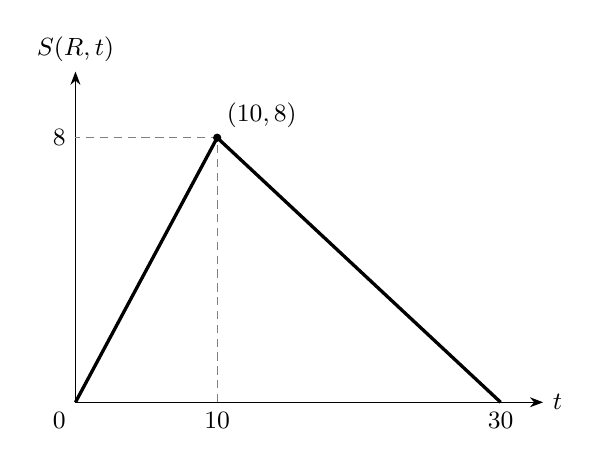
\begin{tikzpicture}[x=.18cm,y=.42cm,>=Stealth,font=\small]
  \draw[->] (0,0)--(33,0) node[right] {$t$};
  \draw[->] (0,0)--(0,10) node[above] {$S(R,t)$};
  \draw[densely dashed,gray] (10,0)--(10,8)--(0,8);
  \draw[very thick] (0,0)--(10,8)--(30,0);
  \fill (10,8) circle (1.5pt);
  \node[above right] at (10,8) {$(10,8)$};
  \node[below left] at (0,0) {$0$};
  \node[below] at (10,0) {$10$};
  \node[below] at (30,0) {$30$};
  \node[left] at (0,8) {$8$};
\end{tikzpicture}
\end{center}
図の太い線が選ばれたエントロピーで、$t=10$で上りから下りに変わる。下りの傾きは上りの半分だから、折れた点の左右で線は対称にならない。
}
\solutionpart{4}{%
$t=0,5,10,20,30$ で
    $S_\emptyset,S_I,S(R)$ の表を作れ。
}{2本の枝 \(S_\emptyset=0.8t\)、\(S_I=12-0.4t\) に五つの時刻を入れる。行ごとに小さいほうを \(S(R)=\min\{S_\emptyset,S_I\}\) として選び、どの行で選ばれる枝が変わるかを見る。}{%
二つの式$S_\emptyset=0.8t$、$S_I=12-0.4t$に、時刻を一つずつ入れる。
\begin{align*}
  t=5&:\ S_\emptyset=4,\quad S_I=12-2=10,\\
  t=20&:\ S_\emptyset=16,\quad S_I=12-8=4,\\
  t=30&:\ S_\emptyset=24,\quad S_I=12-12=0 .
\end{align*}
行ごとに小さいほうを$S(R)$にする。
\[
\begin{array}{c|ccc}
  t&S_\emptyset(t)&S_I(t)&S(R,t)\\ \hline
  0&0&12&0\\
  5&4&10&4\\
  10&8&8&8\\
  20&16&4&4\\
  30&24&0&0
\end{array}
\]
$t=10$までは$S_\emptyset$が選ばれて増える。$t=10$で二つが等しい（Page time）。そのあとは$S_I$が選ばれて減る。
$S(R)$の列だけ見ると、$0\to4\to8\to4\to0$。上がって下がる、Page曲線の形。
}
\solutionpart{5}{%
設問(3)で描いたselected entropyの曲線が
第13章のdimension-counting Page curveと
    同じ形を持ちながら、導出が異なる理由を説明せよ。
}{先月の補習（第13章）で山の形を出すのに何を入力したかを、一つずつ書き出す。この問題で入力したものと並べて、何の小さいほうを選んでいるかと、仮定の種類を比べる。}{%
先月は、蒸発の途中の全体を$\mathcal H_B\otimes\mathcal H_R$に分けて、全体がpureだとした。Schmidt分解から$S_R=S_B$で、それぞれの部分の次元から
\[
 S_R\le\log d_R,\qquad S_R=S_B\le\log d_B
\]
を出した。二つを合わせると$S_R\le\log\min(d_R,d_B)$。ここまでは有限次元の量子力学だけで出る。
でも、pureな状態と次元だけなら、たとえば積の状態の$S_R=0$も許される。だから山の形は、上限だけからは出てこない。
上限にほとんど届く曲線
\[
 S_R\simeq\log\min(d_R,d_B)
\]
を描くには、全体の状態が偏りのない（typicalな）状態だという仮定と、
借りたPage--Senの平均を大きい次元でいちばん粗く読んだ形を使った。
ブラックホールに当てはめるのに足した仮定は、蒸発がunitaryなこと、空間がきれいに掛け算に分かれること、偏りのない状態だということ、の三つ。
先月、小さいほうを選んだのは、二つの部分系の次元。

この問題では、与えられた一般化エントロピーを位置で止めてQESの候補を出して、
その止まった値を比べて
\[
 S(R,t)=\min\{S_\emptyset(t),S_I(t)\}
\]
を出した。この問題で小さいほうを選んだのは、同じ放射$R$のエントロピーを出す二つの候補。
片方が増えて、もう片方が減って、交点で選ばれる枝が入れ替わるから、曲線の形は似てる。
でも、先月のは状態が偏りのないことを仮定した量子情報の模型で、重力は入っていない。
この問題は、半古典の重力の計算で候補を選ぶ順番（止めてから比べる）をまねた模型で、2本の直線も本物の計量から出したものじゃない。
入力が違うから、形が同じになっても、片方の導出がもう片方を確かめたことにはならない。
}
\end{solutionbox}

\begin{solutionbox}{考察　主張の種類を分ける}
次の文を「有限次元量子力学から導出」
「ここで計算」
「重力の標準結果」
「追加仮定」
「ここでは未解決」に分類し、理由を1行ずつ書け。
\solutionpart{1}{%
\(S=\lim_{n\to1}(1-n)^{-1}\log\Tr\rho^n\)。
}{この式を出すのに、重力が要るかどうかを見る。密度行列を固有値で書くと、\(\Tr\rho^n\) は固有値の \(n\) 乗の和になる。そこから \(n\to1\) の極限を取るのに何を使うかを数える。}{%
\begin{quote}
分類：有限次元量子力学から導出。\\
理由：固有値で$\Tr\rho^n=\sum_i\lambda_i^n$と書いてl'Hôpitalを使えば$-\sum_i\lambda_i\log\lambda_i$になり、重力は使わないから。
\end{quote}
以下は確かめ。
密度行列を固有値で書く。$\rho=\sum_i\lambda_i|i\rangle\langle i|$なら$\Tr\rho^n=\sum_i\lambda_i^n$。
$n\to1$では分子$\log\sum\lambda_i^n\to\log1=0$、分母$1-n\to0$で、$0/0$。l'Hôpitalで、分子と分母を$n$で微分する。
\begin{align*}
  \lim_{n\to1}\frac{\log\sum_i\lambda_i^n}{1-n}
  &=\lim_{n\to1}\frac{\sum_i\lambda_i^n\log\lambda_i/\sum_i\lambda_i^n}{-1}
  =-\sum_i\lambda_i\log\lambda_i .
\end{align*}
\[
  S=\lim_{n\to1}\frac{1}{1-n}\log\Tr\rho^n=-\Tr\rho\log\rho
\]
は、密度行列の固有値とl'Hôpitalの規則から出せる。
使ったのは、$\rho$が規格化された正の行列であることだけ。
}
\solutionpart{2}{%
\(\Tr\rho^n=\frac{Z_n}{Z_1^n}\)。
}{規格化する前の \(\widetilde\rho\) と、物理の密度行列 \(\rho=\widetilde\rho/Z_1\) の関係を使う。両辺を \(n\) 乗してtraceを取るだけで済むか、重力の計算まで要るかを見る。}{%
\begin{quote}
分類：ここで計算。\\
理由：$\rho=\widetilde\rho/Z_1$を$n$乗してtraceを取るだけで出て、「unnormalized operatorを正規化する」(2)で確かめたから。
\end{quote}
以下は確かめ。
規格化の関係$\rho=\widetilde\rho/Z_1$から、両辺を$n$乗してtraceを取る。
\begin{equation*}
  \Tr\rho^n=\Tr\frac{\widetilde\rho^{\,n}}{Z_1^n}=\frac{\Tr\widetilde\rho^{\,n}}{Z_1^n}.
\end{equation*}
\[
  \Tr\rho^n=\frac{Z_n}{Z_1^n}
\]
は $\rho=\widetilde\rho/Z_1$ と
$Z_n=\Tr\widetilde\rho^{\,n}$ から代数で確かめた。
$Z_n$を「$n$枚の経路積分を切れ目で縫い合わせたもの」と読むのは、経路積分のいつもの表し方。規格化の$Z_1^n$で割るところは、この章の中で追った。
}
\solutionpart{3}{%
AdS$_3$半円geodesicのlengthは
    \(2L\log(\frac{\ell}{\epsilon})+\cdots\)。
}{二つに分けて見る。半円がいちばん短い線だということを、どこで出したか。その半円の長さ \(2L\log(\ell/\epsilon)\) を、どこで積分したか。}{%
\begin{quote}
分類：ここで計算（入力に、幾何の標準の結果を一つ使う）。\\
理由：半円が測地線であることは借りたが、長さは「AdS$_3$の半円を測る」(1)〜(3)で線素をcutoffのあいだで積分して出したから。
\end{quote}
以下は確かめ。
入力。AdS$_3$のPoincar\'e座標で、境界の区間$[-\ell/2,\ell/2]$の両端をつなぐ測地線は、半円$x^2+z^2=(\ell/2)^2$。これは幾何の標準の結果で、ボードでも借りた。
計算。「AdS$_3$の半円を測る」で、半円の上の線素を出して、cutoffのあいだで積分した。
\begin{equation*}
  \int_{\theta_\epsilon}^{\pi-\theta_\epsilon}\frac{L\,\dd\theta}{\sin\theta}
  =2L\log\cot\frac{\theta_\epsilon}2\simeq2L\log\frac\ell\epsilon .
\end{equation*}
これで
\[
  \Area(\gamma_A)=2L\log(\ell/\epsilon)+\cdots
\]
が出る。
半円が本当に最短（測地線）なことは、ここでは示してない。それを入力にして、長さを出した。
}
\solutionpart{4}{%
gravitational replica path integralは
    replica-connected saddleを含む。
}{つながった鞍点が、どの計算から出てくるかを見る。有限次元の密度行列の代数には、計量もつながり方もない。重力の経路積分で、計量のつながり方まで足すときに出てくるものかどうかを考える。}{%
\begin{quote}
分類：重力の標準結果（条件つき）。\\
理由：重力の経路積分で計量のつながり方まで足すと出てくる鞍点で、制御された低次元の模型では具体的に見つかっているが、有限次元の代数からは出ないから。
\end{quote}
以下は確かめ。
replicaの経路積分は
\begin{equation*}
  Z_n=\int_{\text{境界}=n\ \text{枚}}\mathcal Dg\,\e^{-I[g]}.
\end{equation*}
$n$枚の境界を、それぞれ別の幾何で埋める鞍点と、copyどうしを首でつなぐ鞍点がある（ボードの$n=2$の図の、左と右）。
\begin{equation*}
  Z_n\simeq\underbrace{Z_1^n}_{\text{離れた}}+\underbrace{Z_n^{\text{wormhole}}}_{\text{つながった}}.
\end{equation*}
重力の領域をbathにつないだ、制御された半古典の設定では、二つ目が具体的に出てくる。たとえば、JT重力（2次元の重力の模型。ボードでは名前を出さなかった）をbathにつないだ計算。
でも、どんな境界条件でも必ずあって支配する、という一般の定理じゃない。どのつながり方を足すかと、積分の経路の選び方は、重力の経路積分に置く入力。
}
\solutionpart{5}{%
\(n\to1\) のreplica fixed locusはQES conditionを満たす。
}{QESの条件がどこから来るかを、ボードでたどった順に並べる。途中で置いた前提を数え、その前提を置いたあとの結論が、重力の側で示されたものかを見る。}{%
\begin{quote}
分類：重力の標準結果（前提つき）。\\
理由：replica対称性・固定された面のまわりのなめらかさ・$n$の解析接続を置けば、$n\to1$で固定された面がQESの条件を満たすことが、重力の側で示されているから。
\end{quote}
以下は確かめ。
replica対称な鞍点を$\mathbb Z_n$で割ると、固定された面$\gamma$のまわりの角が$2\pi/n$の幾何になる。欠ける角$2\pi(1-1/n)$は、張力$T_n=\frac{n-1}{4nG}$の面が作る角と同じだった。
ボードでは、張力を持った面の作用を、張力かける面積と読んだ。$n$枚ぶんでは$nT_n\Area(\gamma)=(n-1)\Area(\gamma)/(4G)$で、これが$n\to1$の近くで$nI_1$からずれる1次の項になる。だから
\begin{equation*}
  I_n\simeq n\,I_1+(n-1)\,\frac{\mathrm{Area}(\gamma)}{4G}+\cdots .
\end{equation*}
$\log Z_n\simeq-I_n$として$S=(1-n\partial_n)\log Z_n|_{n=1}$を取ると、面積の項が残る。鞍点の条件（$\gamma$のまわりがなめらかで、運動方程式を満たすこと）は、$\gamma$の位置で面積が止まることになる。量子補正を入れると、それが
\begin{equation*}
  \partial_\gamma\Bigl(\frac{\mathrm{Area}(\gamma)}{4G}+S_{\text{bulk}}\Bigr)=0
\end{equation*}
になる。これがQESの条件。この筋はLewkowycz--Maldacenaの議論から来ていて、ボードでは名前を出さずに使った。
使った前提は、replicaの対称性、固定された面のまわりのなめらかさ、$n$の解析接続。前提なしの有限次元の量子力学からは出ない。
「追加仮定」の分類は、八つの文のどれにも当てていない。設問(4)(5)の文そのものは、前提を置いたあとの結論だから、重力の標準結果にした。追加仮定に当たるのは、その前提のほう（この三つと、設問(4)でどのつながり方を足すか）。
}
\solutionpart{6}{%
islandありcandidateが遅い時刻に必ず全てのblack holeで支配する。
}{「必ず全てのblack holeで」の部分が、分かっている範囲に入っているかを見る。島ありの枝が勝つかどうかは、二つの候補の値を比べて決まる。その値が、ブラックホールごとに何で変わるかを数える。}{%
\begin{quote}
分類：ここでは未解決（一般の主張としては言い過ぎ）。\\
理由：遅い時刻に島ありの枝が勝つことは制御された模型で示されただけで、全部のブラックホールでは示されていないから。
\end{quote}
以下は確かめ。
島ありの枝が選ばれるかは、二つの候補の比べ合い。
\begin{equation*}
  S(R)=\min\bigl\{S_\emptyset(t),\,S_I(t)\bigr\}.
\end{equation*}
それぞれの値は、遠くの境界条件、物質の中身と中心電荷、状態、許す鞍点で決まる。
たとえば設問(4)で挙げた、2次元の重力の模型をbathにつないだ計算では、遅い時刻で$S_I<S_\emptyset$になることが示されている。
でも「全部のブラックホールで必ず」と言うには、全部の場合で$S_I<S_\emptyset$を示さないといけない。そこまでは、まだ示されていない。
}
\solutionpart{7}{%
island formulaがPage curveを与えれば、
    radiationの効率的なdecoding algorithmも得られる。
}{島の公式が出すものと、放射から情報を取り出す手順に要るものを、別々に書き出して比べる。}{%
\begin{quote}
分類：ここでは未解決。\\
理由：島の公式が出すのは$\rho_R$のエントロピーという一つの数で、放射から情報を取り出す操作も、その手間も決めないから。
\end{quote}
以下は確かめ。
島の公式が出すのは、放射の細かいエントロピー一つ。
\begin{equation*}
  S(R)=\min\,\mathrm{ext}_I\Bigl[\frac{\mathrm{Area}(\partial I)}{4G}+S_{\text{bulk}}(R\cup I)\Bigr].
\end{equation*}
これはPage曲線を与えて、情報が失われないことと矛盾しない。
でも取り出すには、放射にかけるユニタリー$V$と、それを作る回路の大きさが要る。エントロピーは$\rho_R$の固有値しか見ていないから、$V$は決まらない。
ボードの五つの注意の三つ目（Page曲線が描けても、放射から投入した情報を効率よく取り出せることにはならない）と同じ。
補足として、取り出すのにかかる手間が、ブラックホールのエントロピーの指数関数くらいまで大きくなりうる、という議論もある（HarlowとHaydenによる。この補習では扱っていない）。
}
\solutionpart{8}{%
asymptotically flatな4次元black holeの情報問題は完全に解決した。
}{島の計算が制御できている模型と、遠くが平らな4次元の現実の蒸発を分ける。前者でPage曲線が出たことは大事な証拠。後者で何がまだ作られていないかを書き出す。}{%
\begin{quote}
分類：ここでは未解決。\\
理由：bathにつないだ制御された模型ではPage曲線が出たが、遠くが平らな4次元の蒸発では、摂動に頼らない量子重力の時間発展がまだ作られていないから。
\end{quote}
以下は確かめ。
島の計算で分かっていることと、まだのことを並べる。
\begin{align*}
  \text{できた}&:\ \text{bathにつないだ低次元の制御された模型で、}S(R)\ \text{がPage曲線になる},\\
  \text{まだ}&:\ \text{4次元の遠くが平らな蒸発で、摂動に頼らない量子重力の時間発展全部}.
\end{align*}
4次元の平らな場合は、遠くで重力を切れないし、放射を集めるbathの置き方も自然じゃない。島の計算をそのまま当てはめるには、まだ仮定が要る。
ボードの五つの注意の五つ目と同じ。
だから、情報問題の大事な前進だけど、完全に解けた、とは言わない。
}
\solutionfollowup{最後に、island formulaを「内部を手で足す規則」と読むのが不十分な理由を説明せよ。}{「手で足す規則」と読んだとき、島の公式のどの段が説明できなくなるかを挙げる。それぞれの段が、重力の経路積分のどこから出てくるかを、設問(4)(5)と同じ順で対応させる。}{%
island formulaを「内側を手で足す規則」と読むと、
なんで $I$ が候補に入るのか、なんでその境界を止めるのか、
なんで候補の中から最小を選ぶのかが、説明できない。
いつもの重力のreplicaの計算では、
\[
  Z_n\simeq\sum_s\e^{-I_n^{(s)}}
\]
に、replicaが離れた鞍点だけじゃなくて、
replicaがつながったwormholeの鞍点も入れる。
三つの段は、ここから順に出てくる。
候補に$I$が入るのは、つながった鞍点が、離れた鞍点とは別のエントロピーの候補を与えるから。
境界を止めるのは、設問(5)のとおり、$n\to1$で固定された面のまわりがなめらかで運動方程式を満たす、という鞍点の条件がQESの条件になるから。
最小を選ぶのは、$I_n^{(s)}-nI_1\simeq(n-1)S_n^{(s)}$で、$n>1$では作用の小さい鞍点ほど$S_n^{(s)}$も小さく、その鞍点が$\e^{-I}$の和でいちばん大きい寄与をするから（そのまま$n\to1$まで延ばせるとして）。
だから島は、勝手に足した領域じゃなくて、
\[
  {\text{別topologyのgravitational saddleが残すentropy candidate}}
\]
として読む。千奈がボードで言った「別の鞍点の跡」のこと。
}
\end{solutionbox}


\clearpage
\endgroup
\begingroup
\renewcommand{\runningtitle}{解答 第15章　量子重力とswampland}
\newcommand{\Mpl}{M_{\mathrm{Pl}}}
\newcommand{\Lsp}{\Lambda_{\mathrm{sp}}}
\newcommand{\mtower}{m_{\mathrm{tower}}}
\renewcommand{\runningtitle}{解答 第15章　量子重力とswampland}
\section[量子重力の条件とswampland　課題解答]{量子重力の条件とswampland──課題解答}
\subsection{書けるけど、存在できない──解答}

ホワイトボードの右半分から予算の申請書が1枚ずつ減っていった週に、広は最後の宿題を8問出した。
答案を返すときには、1問ずつ、解き方を書いた紙を添えた。

\begin{solutionbox}{確認　有効作用の次元}
4次元の作用
\[
  S=\int\dd^4x\sqrt{-g}\left[
    \frac{\Mpl^2}{2}\mathcal R
    -\frac12(\partial\phi)^2
    -V(\phi)
    -\frac1{4g^2}F^2
  \right]
\]
を考える。
\solutionpart{1}{%
$[\partial_\mu]=1$、作用が無次元であることから、
    $\Mpl,\phi,A_\mu,V,g$ の質量次元を求めよ。
}{作用に単位がないことから、まずLagrangianの密度の質量次元が決まる。そのあと、Einstein--Hilbertの項、scalarの運動項、ゲージの運動項を一つずつ見て、\(\Mpl,\phi,A_\mu,g\) を出す。potentialは、括弧の中で運動項と並んでる項だから、密度と同じ次元を持つ。}{%
自然単位では作用に単位がなくて、
\[
  [\dd^4x]=-4,
  \qquad
  [\mathcal L]=4.
\]
微分は $[\partial_\mu]=1$。$\mathcal R$は計量の2階微分でできてるから、$[\mathcal R]=2$。

Einstein--Hilbertの項から
\[
  [\Mpl^2]+[\mathcal R]
  =
  2[\Mpl]+2
  =
  4
\]
だから
\[
  {[\Mpl]=1}.
\]
scalarの運動の項は、微分が二つと$\phi$が二つ。
\[
  2+2[\phi]=4
\]
だから
\[
  {[\phi]=1}.
\]

$F_{\mu\nu}=\partial_\mu A_\nu-\partial_\nu A_\mu$ だから
\[
  [F_{\mu\nu}]=1+[A_\mu].
\]
電荷$q$を整数にしたこの書き方では、$A_\mu$は共変微分$\partial_\mu-\imunit qA_\mu$の中で$\partial_\mu$と足し合わさるから、$[A_\mu]=[\partial_\mu]=1$。$F^2$の次元を数えると
\[
  2(1+[A_\mu])=4,
\]
で、$F^2$だけで4がそろう。前の$1/g^2$には単位が残らない。
だから
\[
  {[A_\mu]=1,\quad[F_{\mu\nu}]=2,\quad[g]=0}.
\]
potentialはLagrangianの密度と同じ次元だから
\begingroup\postdisplaypenalty=10000
\[
  {[V]=4}.
\]
\endgroup
}
\solutionpart{2}{%
$V=\mu^4 f(\frac{\phi}{f_0})$ と書くとき、
    $\mu$ と $f_0$ の質量次元を求めよ。
}{関数 \(f\) の中身 \(\phi/f_0\) には単位がないこと。potential全体は質量次元4。この二つを別々に使って、\(f_0\) と \(\mu\) の次元を出す。}{%
一つ目の条件。関数$f$の中身は無次元。たとえば$f(u)=\cos u$や$u^2$で、$u$に単位があると、$\cos u$の展開の項どうしで単位がそろわない。
\begin{equation*}
  \left[\frac{\phi}{f_0}\right]=0
  \quad\Longrightarrow\quad
  [f_0]=[\phi]=1 .
\end{equation*}
4次元の正準scalarは$[\phi]=1$（設問(1)）。

二つ目の条件。potentialはLagrangianの密度と同じ次元で$[V]=4$。$f$は無次元の数だから、次元は全部$\mu^4$が持つ。
\begin{equation*}
  [\mu^4]=4
  \quad\Longrightarrow\quad
  [\mu]=1 .
\end{equation*}
\[
  V=\mu^4 f(\phi/f_0)
\]
だから
\[
  {[\mu]=1,\qquad[f_0]=1}.
\]
$\mu$はpotentialの高さの目盛り、$f_0$は場の値の目盛り。potentialが周期的なaxionは、まだ扱ってない。たとえばそういうaxionなら、$f_0$は崩壊定数と呼ばれて、potentialの周期は$2\pi f_0$になる。
}
\solutionpart{3}{%
Distance Conjecture、WGC、de Sitter conjectureが、
    それぞれ作用のどの係数を主に調べるか答えよ。
}{三つの予想が、それぞれ何についての主張だったかを思い出す。それを、作用の項（Einstein--Hilbert、scalarの運動項、potential、ゲージの運動項）のどれの係数の話かに対応させる。最初の日に作用の下に書いた表が、手がかりになる。}{%
作用の項ごとに並べる。
\begin{center}
\small
\begin{tabularx}{.92\linewidth}{>{\bfseries\sffamily}p{.31\linewidth}X}
\toprule
条件 & 主に調べる量\\
\midrule
Distance Conjecture &
scalar kinetic termの $G_{ij}(\phi)$ とfield-space distance。\\
Weak Gravity Conjecture &
gauge coupling $g$、整数charge $q$、state mass $m$。\\
de Sitter conjecture &
potential $V$、gradient $\nabla_iV$、Hessian $\nabla_i\nabla_jV$。\\
\bottomrule
\end{tabularx}
\end{center}
}
\end{solutionbox}

\begin{solutionbox}{誘導付き　円半径と無限距離}
\[
  \varphi=\sqrt{\frac32}\Mpl\log\left(\frac{R}{R_0}\right),
  \quad
  m_n^{\mathrm{KK}}=\frac{|n|}{R}\sqrt{\frac{R_0}{R}}
\]
を使う。設問(1)(2)は4次元Einstein frameの量。
設問(3)(4)では第8章のstring frameへ戻り、$\alpha'$を固定して
$m_w^{\mathrm{wind}}=|w|R/\alphap$、$m_{n,\mathrm S}^{\mathrm{KK}}=|n|/R$を使う。
\solutionpart{1}{%
$R_2=aR_1$（$a>1$）のfield distanceを求めよ。
}{問題文の \(\varphi\) は正準に規格化したscalarだから、場の距離は \(\varphi\) の差を \(\Mpl\) で割ったもの。二つの半径での \(\varphi\) を引き算して、\(R_2=aR_1\) を入れる。\(a>1\) を使うのは、絶対値を外すところ。}{%
与えられた式は$\varphi=\sqrt{3/2}\,\Mpl\log(R/R_0)$。二つの半径での値を引くと、$R_0$は消える。
\begin{align*}
  \Delta\varphi
  &=\sqrt{\frac32}\Mpl\left[\log\frac{R_2}{R_0}-\log\frac{R_1}{R_0}\right]
  =\sqrt{\frac32}\Mpl\log\frac{R_2}{R_1}.
\end{align*}
$\Mpl$で割って、絶対値を取る。$R_2=aR_1$を入れる。
\begin{align}
  \frac{|\Delta\varphi|}{\Mpl}
  &=
  \sqrt{\frac32}
  \left|
    \log\frac{R_2}{R_1}
  \right|
  =\sqrt{\frac32}\,|\log a|
  ={\sqrt{\frac32}\log a}.
  \label{ls17-eq:sol17-radius-distance}
\end{align}
$a>1$なら$\log a>0$で、絶対値はそのまま外れる。
場の距離は、半径の比の対数。半径を$\e$倍にするたびに、$\sqrt{3/2}\simeq1.22$ Planck単位進む。
}
\solutionpart{2}{%
設問(1)で得た
$\frac{|\Delta\varphi|}{\Mpl}=\sqrt{3/2}\log a$
に
    $a=\e^{10\sqrt{2/3}}$ を代入したとき、
    $\frac{|\Delta\varphi|}{\Mpl}$ と
    $\frac{m_1^{\mathrm{KK}}(R_2)}{m_1^{\mathrm{KK}}(R_1)}$ を求めよ。
}{距離は、設問(1)の式に \(\log a=10\sqrt{2/3}\) を入れるだけ。質量の比は、問題文のKKの質量が \(R\) の何乗に比例するかを読む。円の運動量 \(|n|/R\) だけを見ると、Einstein frameに移すときの因子 \(\sqrt{R_0/R}\) を落とす。佑芽がボードで最初に書いた \(\e^{-\sqrt{2/3}\,\Delta}\) は、この因子を落とした形。}{%
$\log a=10\sqrt{2/3}$だから、設問(1)の式で
\[
  \frac{|\Delta\varphi|}{\Mpl}
  =\sqrt{\frac32}\times10\sqrt{\frac23}
  =10 ,
\]
つまり
\[
  {\frac{|\Delta\varphi|}{\Mpl}=10}.
\]
KKの質量には、Einstein frameに移す因子$\sqrt{R_0/R}$も入って、全体で$R^{-3/2}$に比例する。$n=1$で比を取ると、$R_0$も消える。
\begin{align}
  \frac{
    m_1^{\mathrm{KK}}(R_2)}
  {m_1^{\mathrm{KK}}(R_1)}
  &=
  \left(\frac{R_1}{R_2}\right)^{3/2}
  =
  a^{-3/2}
  \nonumber\\
  &=
  {\e^{-10\sqrt{3/2}}}.
\end{align}
指数は$\frac32\times10\sqrt{2/3}=10\sqrt{3/2}$。数にすると$4.8\times10^{-6}$くらいで、場の距離を10進むあいだに、いちばん軽いKKの粒子は1001万分の5くらいの重さになる。
}
\solutionpart{3}{%
設問(1)と同じ半径変化$R_2=aR_1$について、
$\frac{m_1^{\mathrm{wind}}(R_2)}{m_1^{\mathrm{wind}}(R_1)}$を求めよ。
}{巻きつきの質量 \(m_w^{\mathrm{wind}}=|w|R/\alpha'\) で、半径への依存を読む。\(\alpha'\) は固定だから、比を取ると消える。}{%
string frameで、$\alphap$を固定する。巻きつきの質量は
\begin{equation*}
  m_w^{\mathrm{wind}}=\frac{|w|R}{\alphap},
\end{equation*}
で、半径に比例する。$w=1$で、二つの半径の比を取ると$\alphap$が消える。
\[
  \frac{
    m_1^{\mathrm{wind}}(R_2)}
  {m_1^{\mathrm{wind}}(R_1)}
  =
  \frac{R_2/\alphap}{R_1/\alphap}
  =
  \frac{R_2}{R_1}
  =
  {a}.
\]
ひもを巻きつける円が長くなるから、伸ばした分だけ重い。
同じ半径の変化で、KKの段（$\propto1/R$）は軽く、巻きつきの段（$\propto R$）は重くなる。
だから、$R$をどっちの向きに無限に動かしても、どっちかの段が軽くなってくる。Distance Conjectureの典型の例。

ただ、ここの質量はstring frameで$\alphap$を固定して測ったもの。設問(2)の4次元Einstein frameの質量とは物差しが違うから、この比$a$と設問(2)の$a^{-3/2}$を並べて、指数の係数を読み比べることはできない。
}
\solutionpart{4}{%
$R\to0$ で軽くなるtowerを答え、
    $R\leftrightarrow\frac{\alphap}{R}$ が二つのtowerをどう交換するか示せ。
}{KKの質量 \(m_n=|n|/R\) と、巻きつきの質量 \(m_w=|w|R/\alpha'\) の、\(R\) への依存を比べる。交換のほうは、双対の半径 \(\widetilde R=\alpha'/R\) で巻きつきの質量を書き直して、どの形になるかを見る。}{%
\[
  m_w^{\mathrm{wind}}=\frac{|w|R}{\alphap}
\]
だから $R\to0$ で巻きつきの段が軽くなる。KKの段$|n|/R$は、逆に重くなる。

双対の半径を
\[
  \widetilde R=\frac{\alphap}{R}
\]
とすると
\[
  \frac{|w|R}{\alphap}
  =
  \frac{|w|}{\widetilde R}.
\]
元の巻きつきの数 $w$ は、双対の側の運動量の数として読める。
同じように、$|n|/R=|n|\widetilde R/\alphap$だから、元の運動量の数 $n$ は双対の側の巻きつきの数になる。
\[
  {
  R\longleftrightarrow\frac{\alphap}{R},
  \qquad
  n\longleftrightarrow w}.
\]
小さい半径で軽くなる巻きつきの段は、双対の大きい半径$\widetilde R$で軽くなるKKの段と、同じ質量の並び。
}
\end{solutionbox}

\begin{solutionbox}{本気　towerがcutoffを下げる}
等間隔tower $m_n=n\mtower$ を考え、
\[
  N(\Lsp)\simeq\frac{\Lsp}{\mtower},
  \qquad
  \Lsp\simeq\frac{\Mpl}{\sqrt N}
\]
と見積もる。
\solutionpart{1}{%
$\Lsp$ を $\Mpl,\mtower$ で表せ。
}{cutoffより下にある等間隔の段の種類の数を \(N\simeq\Lsp/\mtower\) と数えて、species bound \(\Lsp\simeq\Mpl/\sqrt N\) に入れる。\(\Lsp\) が両辺に出てくる式を解いて、\(\Mpl\) と段の間隔で書く。}{%
\[
  N\simeq\frac{\Lsp}{\mtower}
\]
をspecies boundに入れる。
\begin{align}
  \Lsp
  &\simeq
  \frac{\Mpl}{
    \sqrt{\Lsp/\mtower}},
  \\
  \Lsp^{3/2}
  &\simeq
  \Mpl\mtower^{1/2}.
\end{align}
両辺を $2/3$ 乗して
\begin{equation}
  {
  \Lsp
  \simeq
  \left(\Mpl^2\mtower\right)^{1/3}}.
  \label{ls17-eq:sol17-species-scale}
\end{equation}
\answerconclusion{等間隔の塔1本だけを数えた自己無撞着なspecies cutoffは
$\Lsp\simeq(\Mpl^2\mtower)^{1/3}$。$\Mpl$が二つと$\mtower$が一つの、3乗根。}
}
\solutionpart{2}{%
$\mtower=m_0\e^{-\alpha\Delta}$ のとき、
    $\frac{\Lsp(\Delta)}{\Lsp(0)}$ を求めよ。
}{設問(1)の \(\Lsp\simeq(\Mpl^2\mtower)^{1/3}\) に、Distance Conjectureの形の \(\mtower(\Delta)=m_0e^{-\alpha\Delta}\) を入れる。最初の \(\Delta=0\) との比を取ると、\(\Mpl\) と \(m_0\) が消える。}{%
\[
  \mtower(\Delta)=m_0\e^{-\alpha\Delta}
\]
を設問(1)の $\Lsp\simeq(\Mpl^2\mtower)^{1/3}$ に入れると
\[
  \Lsp(\Delta)
  \simeq
  (\Mpl^2m_0)^{1/3}
  \e^{-\alpha\Delta/3}.
\]
$\Delta=0$では$(\Mpl^2m_0)^{1/3}$だから、割って
\[
  {
  \frac{\Lsp(\Delta)}{\Lsp(0)}
  =
  \e^{-\alpha\Delta/3}}.
\]
\answerconclusion{towerが $\e^{-\alpha\Delta}$ で軽くなると、cutoffは指数が3分の1の
$\e^{-\alpha\Delta/3}$ で下がる。}
}
\solutionpart{3}{%
$\alpha=\frac{1}{\sqrt3}$、$\Delta=12$ のとき、
    tower massとspecies cutoffがそれぞれ何倍になるか、
    指数の形で答えよ。
}{段の質量の比 \(e^{-\alpha\Delta}\) と、species cutoffの比 \(e^{-\alpha\Delta/3}\) を使う。それぞれに \(\alpha=1/\sqrt3\)、\(\Delta=12\) を入れて、指数を整理して、下がる速さを比べる。}{%
指数は$\alpha\Delta=12/\sqrt3=4\sqrt3$。段の質量は
\[
  {
  \frac{\mtower(12)}{\mtower(0)}
  =
  \e^{-12/\sqrt3}
  =
  \e^{-4\sqrt3}}
\]
倍になる。species cutoffは、指数がその3分の1で
\[
  {
  \frac{\Lsp(12)}{\Lsp(0)}
  =
  \e^{-12/(3\sqrt3)}
  =
  \e^{-4/\sqrt3}}
\]
倍になる。数の目安はそれぞれ、だいたい
\[
  9.8\times10^{-4},
  \qquad
  9.9\times10^{-2}.
\]
段の質量は1000分の1くらいまで下がるけど、cutoffは10分の1くらい。
\answerconclusion{tower massは $\e^{-4\sqrt3}$ 倍、species cutoffは
$\e^{-4/\sqrt3}$ 倍。}
}
\solutionpart{4}{%
設問(1)から設問(3)で用いた
species cutoffの見積もりが正確な等号でない理由を二つ挙げよ。
}{問題文の2本の見積もり、段の数 \(N\simeq\Lsp/\mtower\)（設問(1)で使った）と、species bound \(\Lsp\simeq\Mpl/\sqrt N\) の、それぞれで何を捨てたかを点検する。段の数え方の単純化と、係数や相互作用の省略を、別々の理由として挙げる。}{%
見積もりの2本は、どっちも$\simeq$で書いてた。何を捨てたかを、二つ挙げる。
\begin{enumerate}
  \item 段の数え方を単純にしてる。$N\simeq\Lsp/\mtower$は、levelごとに1種類の粒子と数えてる。本当は、levelごとに偏極やいくつかの場があって（縮退）、KKとひもの振動みたいに違う種類の段が重なることもある。levelを数えるときの端の扱い（$\lfloor\cdot\rfloor$）も落としてる。
  \item species boundの係数を捨ててる。$\Lsp=\Mpl/\sqrt N$の前の1くらいの係数（Planck質量の規約による$\sqrt{8\pi}$や、$4\pi$のような因子）は決めてない。
\end{enumerate}
ほかに、cutoffの近くでの相互作用を挙げてもいい。$\Lsp$に近いところでは重力がもう強くて、段の粒子を自由な粒子として数える前提が崩れる。

だから設問(1)--(3)で言えるのは、$\Lsp$が$\mtower$のどのべきで動くか（$1/3$乗）、まで。係数は決めてない。
}
\end{solutionbox}

\begin{solutionbox}{誘導付き　二つの力を比べる}
同じmass $m$、charge $q$ の粒子二つについて
\[
  V_{\mathrm{gauge}}=\frac{g^2q^2}{4\pi r},
  \qquad
  V_{\mathrm{grav}}=-\frac{m^2}{8\pi\Mpl^2r}
\]
とする。
\solutionpart{1}{%
net long-range forceが斥力または0となるmass boundを導け。
}{同じ符号の電荷のゲージの反発 \(g^2q^2/(4\pi r)\) と、重力の引力 \(-m^2/(8\pi\Mpl^2r)\) を足す。力の向きは、足したpotentialを \(r\) で微分した \(F_r=-\dd V/\dd r\) の符号で決める。}{%
全体のpotentialは
\begin{align}
  V_{\mathrm{net}}(r)
  &=
  \frac{g^2q^2}{4\pi r}
  -
  \frac{m^2}{8\pi\Mpl^2r}
  \nonumber\\
  &=
  \frac1{4\pi r}
  \left(
    g^2q^2
    -
    \frac{m^2}{2\Mpl^2}
  \right).
\end{align}
potentialの符号を力の向きにつなげたいから、距離$r$で微分する。
二つの粒子が離れる向きを正にした、動径の方向の力は
\[
 F_r=-\frac{\dd V_{\mathrm{net}}}{\dd r}
 =\frac1{4\pi r^2}
 \left(g^2q^2-\frac{m^2}{2\Mpl^2}\right).
\]
$r>0$だから、反発かゼロ、つまり$F_r\ge0$は、括弧の中が負じゃないことと同じ。$r$は括弧の外にしかないから、条件はどの距離でも同じ。
\[
  g^2q^2
  \ge
  \frac{m^2}{2\Mpl^2}.
\]
$m>0$で平方根を取って
\[
  {
  m\le\sqrt2g|q|\Mpl}.
\]
}
\solutionpart{2}{%
設問(1)で導いた
$m\le\sqrt2g|q|\Mpl$
を
    \[
      z=\frac{\sqrt2g|q|\Mpl}{m}
    \]
    で書き換え、$z=2,\ 1,\ \frac{1}{2}$ を分類せよ。
}{設問(1)の上限の両辺を \(m\) で割って、\(z\) と1の大小の条件にする。\(z\) が1より大きい、等しい、小さいを、ゲージの反発と重力の引力のどっちが強いかに対応させる。}{%
設問(1)の不等式を$m$で割ると
\[
  z=\frac{\sqrt2g|q|\Mpl}{m}\ \ge\ 1 .
\]
設問(1)の$F_r$の括弧は$\frac{m^2}{2\Mpl^2}(z^2-1)$と書けるから、反発と引力の大きさの比は$z^2$。
\begin{center}
\begin{tabular}{ccl}
\toprule
$z$ & 分類 & net force\\
\midrule
$2$ & superextremal & gauge repulsionが強い\\
$1$ & extremal & 長距離で釣り合う\\
$1/2$ & subextremal & gravity attractionが強い\\
\bottomrule
\end{tabular}
\end{center}
極限のblack holeは、$M_{\mathrm{ext}}=\sqrt2g|Q|\Mpl$を入れるとちょうど$z=1$。三つの名前は、これと比べた呼び方。
}
\solutionpart{3}{%
$g=10^{-2}$、$q=1$ のとき、
    WGC境界のmassを $\Mpl$ 単位で求めよ。
}{WGCの境目、つまり力がつり合う \(m=\sqrt2g|q|\Mpl\) を使う。\(g=10^{-2}\)、\(|q|=1\) を入れて、\(\Mpl\) を単位にした数にする。}{%
WGCの境目は、力がつり合う$z=1$。
\begin{equation*}
  m_{\mathrm{boundary}}=\sqrt2\,g|q|\Mpl .
\end{equation*}
$g=10^{-2}$、$q=1$を入れる。
\[
  m_{\mathrm{boundary}}
  =
  \sqrt2\times10^{-2}\times1\times\Mpl
  =\sqrt2\times10^{-2}\Mpl.
\]
$\sqrt2\simeq1.414$だから
\[
  {
  m_{\mathrm{boundary}}
  \simeq1.41\times10^{-2}\Mpl}.
\]
$\Mpl\simeq2.4\times10^{18}\ \mathrm{GeV}$（換算Planck質量）なら、$3\times10^{16}\ \mathrm{GeV}$くらい。
WGCは、これより軽い電荷1の粒子が少なくとも一つある、と言う。電子は$g\sim0.3$で、質量は$5\times10^{-4}\ \mathrm{GeV}$くらい。佑芽が電卓で出したとおり$z_e\approx2\times10^{21}$で、境目をはるかに越えてる。
\answerconclusion{この規格化で、WGCの境目のmassは
$m_{\mathrm{boundary}}\simeq1.41\times10^{-2}\Mpl$。}
}
\solutionpart{4}{%
「全荷電粒子が設問(1)の
$m\le\sqrt2g|q|\Mpl$を満たす」が
    最小のelectric WGCより強い理由を説明せよ。
}{いちばん弱いelectric WGCが、荷電状態のうちどれだけに条件を課してるかをはっきりさせる。二つの文を、量化の記号で書き分けてから比べる。}{%
いちばん弱いelectric WGCは
\[
  \exists\,(m,q):\quad z\ge1
\]
という、「ある」の命題。
「全部の荷電粒子が上限を満たす」は
\[
  \forall\,(m,q):\quad z\ge1
\]
という「全部」の命題で、下回る荷電状態を一つも許さない。

荷電粒子が一つでもいる理論なら、「全部」が成り立てば「ある」も成り立つ。逆は成り立たない。たとえば$z=2$の粒子と$z=1/2$の粒子が一つずつある理論は、いちばん弱いWGCを満たすけど、「全部」の形は破る。だから「全部」のほうがはっきり強くて、いちばん弱いWGCはそこまで言ってない。
}
\end{solutionbox}

\begin{solutionbox}{本気　極限black holeを1段放電させる}
\[
  M_{\mathrm{ext}}(Q)=\sqrt2gQ\Mpl,
  \qquad Q>q>0
\]
とする。extremal black holeがmass $m$、charge $q$ の粒子を一つ放出する。
\solutionpart{1}{%
最終black holeのchargeを書け。
}{粒子が1個、電荷 \(q\) を持って出ていくときに、電荷の保存を使う。最初の電荷 \(Q\) から出ていく \(q\) を引いて、最後のblack holeの電荷を書く。}{%
電荷は保存する。粒子を一つ出す前と後で、全部の電荷は同じ。
\begin{equation*}
  \underbrace{Q}_{\text{前}}=\underbrace{Q_{\mathrm f}}_{\text{後のblack hole}}+\underbrace{q}_{\text{出ていった粒子}} .
\end{equation*}
電荷の保存を「最初の電荷 $=$ 最後の電荷 $+$ 出ていった電荷」と書くと
\begin{align}
  Q&=Q_{\mathrm f}+q,\\
  Q_{\mathrm f}&=Q-q.
\end{align}
$Q>q>0$だから、最後のblack holeも正の電荷を持ってる。同じ符号の電荷を一つ外に出して、電荷が$q$だけ減った。
\answerconclusion{最終black holeのchargeは $Q_{\mathrm f}=Q-q$ で、まだ正。}
}
\solutionpart{2}{%
energy conservationと最終black holeのextremal boundから
    \[
      M_{\mathrm{ext}}(Q)
      \ge m+M_{\mathrm{ext}}(Q-q)
    \]
    を使い、$m$ の条件を求めよ。
}{最初と最後のblack holeにextremalな質量 \(M_{\mathrm{ext}}(Q)=\sqrt2g|Q|\Mpl\) を使って、出ていく粒子の静止質量も入れたenergyの保存の不等式に入れる。\(Q>q>0\) で絶対値を外して、両辺に共通の項を引く。}{%
energyの保存。止まったblack holeの質量（最初のenergy）が、出た粒子の静止質量と、残ったblack holeの質量以上でないといけない。運動のenergyは負にならないから、不等式になる。
\begin{align}
  M_{\mathrm{ext}}(Q)
  &\ge
  m+M_{\mathrm f}.
\end{align}
残ったblack holeは、電荷$Q-q$のextremalの質量より軽くはなれない（それより軽いと、裸の特異点）。だから$M_{\mathrm f}\ge M_{\mathrm{ext}}(Q-q)$で、いちばん得な場合を入れると
\begin{align}
  M_{\mathrm{ext}}(Q)
  &\ge
  m+M_{\mathrm{ext}}(Q-q),
  \\
  \sqrt2gQ\Mpl
  &\ge
  m+\sqrt2g(Q-q)\Mpl.
\end{align}
両辺から $\sqrt2g(Q-q)\Mpl$ を引くと、$Q$が消えて
\[
  \sqrt2gQ\Mpl-\sqrt2g(Q-q)\Mpl=\sqrt2gq\Mpl\ \ge\ m ,
\]
\[
  {
  m\le\sqrt2gq\Mpl}.
\]
「二つの力を比べる」の設問(1)で、力から出した境目と同じ形。ボードの右半分で千奈が出した1行も、これだった。

この計算には、向きの違う不等式が二つ出てくる。$M_{\mathrm f}\ge M_{\mathrm{ext}}(Q-q)$は、残ったblack holeがblack holeでいるための下限。出ていく粒子に課されるのは、上限$m\le\sqrt2gq\Mpl$。extremalなblack holeが崩れていけるには、電荷と質量の比が、black hole自身より大きい粒子がいる。
}
\solutionpart{3}{%
$m$が設問(2)で得たboundを厳しく上回る場合、
粒子1個を放出する1段放電が運動学的に許されないことを示せ。
}{設問(2)の条件の逆 \(m>\sqrt2gq\Mpl\) を仮定する。この不等式の両辺に、最後のextremalなblack holeの質量を足す。足した結果を、最初のblack holeの質量と比べる。}{%
もし
\[
  m>\sqrt2gq\Mpl
\]
なら
\begin{align}
  m+M_{\mathrm{ext}}(Q-q)
  &>
  \sqrt2gq\Mpl
  +
  \sqrt2g(Q-q)\Mpl
  \nonumber\\
  &=
  \sqrt2gQ\Mpl
  =
  M_{\mathrm{ext}}(Q).
\end{align}
左辺は、放電のあとの静止質量のいちばん小さい値。残ったblack holeは$M_{\mathrm{ext}}(Q-q)$より軽くなれないし、運動のenergyは足されるだけだから、あとのenergyは左辺以上になる。それが最初の質量$M_{\mathrm{ext}}(Q)$を越えるから、
この1段の放電はenergyの保存と両立しない。粒子が重すぎて、出ていけない。
}
\solutionpart{4}{%
設問(2)で用いたenergy inequalityだけでは
decay rateを求められない理由を説明せよ。
}{energyの不等式が決めるのは、最後の状態に行けるかどうかの二択。崩壊の速さには、時間あたりに何が起きるかを決める量が要る。そういう量が不等式に入ってるかを見る。}{%
不等式は、最後の状態に行けるだけのenergyの余裕があるかを決めるだけ。時間あたりに何回起きるかは、入ってない。
本当の速さには、少なくとも
\begin{itemize}
  \item black-hole backgroundで、粒子が作られる振幅、
  \item black holeのまわりの重力のpotentialの山を、粒子が抜けて遠くまで届く割合（跳ね返されて戻る分を除いた割合で、greybody factorと呼ぶ）、
  \item 角運動量と、出ていく粒子がblack holeの時空を変える効果（backreaction）
\end{itemize}
が要る。どれも、静止質量と電荷の勘定には出てこない量。だから、行けると分かっても、速さは決まらない。
}
\end{solutionbox}

\begin{solutionbox}{比較　global symmetryへ近づけるか}
magnetic WGCのparametric cutoff
\[
  \Lambda\lesssim g\Mpl
\]
を仮定する。
\solutionpart{1}{%
fixed experimental energy $E=10^{-6}\Mpl$ をEFT内に保つには、
    $g$ にどんな下限が必要か。
}{実験を有効理論で書く条件 \(E<\Lambda\) と、magnetic WGCのcutoff \(\Lambda\lesssim g\Mpl\) を一緒に課す。決めたenergy \(E=10^{-6}\Mpl\) がcutoffより下に入るための、\(g\) の大きさの下限を出す。}{%
二つの条件を並べる。
\begin{itemize}
  \item 実験を有効理論で書けるには、energyがcutoffより下：$E<\Lambda$。
  \item magnetic WGCの上限：$\Lambda\lesssim g\Mpl$。
\end{itemize}
つなぐと
\[
  E<\Lambda\lesssim g\Mpl
\]
を一緒に満たすには、大きさとしては
\[
  g\gtrsim\frac{E}{\Mpl}=\frac{10^{-6}\Mpl}{\Mpl}=10^{-6}.
\]
だから
\[
  {g\gtrsim10^{-6}}
\]
が要る。$\lesssim$で書いた上限だから、1くらいの係数は決めてない。
gaugeの結合が$10^{-6}$より弱いと、新しい物理が出てくるenergy（cutoff）が、$10^{-6}\Mpl$の実験のenergyより下に来る。
}
\solutionpart{2}{%
$g=10^{-8}$へ下げたとき、
設問(1)のfixed energy $E=10^{-6}\Mpl$の実験を
EFTだけで記述できるか。
}{magnetic WGCの \(\Lambda\lesssim g\Mpl\) に \(g=10^{-8}\) を入れる。出てきたcutoffの上限と、設問(1)の決めた実験のenergy \(E=10^{-6}\Mpl\) を比べる。}{%
magneticのcutoffに$g=10^{-8}$を入れる。
\[
  \Lambda\lesssim g\Mpl=10^{-8}\Mpl.
\]
実験のenergyと比べる。
\[
  \frac{E}{\Lambda}\gtrsim\frac{10^{-6}\Mpl}{10^{-8}\Mpl}=10^2 .
\]
\[
  E=10^{-6}\Mpl>\Lambda
\]
だから、この有効理論だけでは同じ実験を書けない。
実験はcutoffより100倍以上高いenergyで、$g=10^{-8}$は設問(1)の下限$g\gtrsim10^{-6}$を2桁下回ってる。

cutoffより下に、新しい自由度か、別の書き方が要る。magnetic WGCの見積もりでは、モノポールの芯の大きさ$1/\Lambda$のところで、この$U(1)$の有効理論に入ってない新しい物理（荷電状態の塔や、ひもなど）が出てくる。モノポール自身は$m_{\mathrm{mon}}\sim\Lambda/g^2$で、$\Lambda$より$1/g^2=10^{16}$倍くらい重いから、$\Lambda$のあたりにはまだ出てこない。
}
\solutionpart{3}{%
$g\to0$ で固定cutoffを保てないことを式で示せ。
}{magneticのcutoffの関係 \(\Lambda\lesssim g\Mpl\) で、\(\Mpl\) を固定して \(g\to0\) にする。そのとき上限がどこへ行くかを書いて、決めた実験のenergy \(E>0\) と比べる。}{%
$\Mpl$を固定すると
\[
  \lim_{g\to0}g\Mpl=0
\]
だから、cutoffの上限がゼロに近づく。$\lesssim$は係数を捨てた大きさの関係なので、言えるのは大きさとして
\[
  \lim_{g\to0}\Lambda=0 .
\]
どんな決めた $E>0$ でも、$g$ が十分小さければ（大きさとして$g\lesssim E/\Mpl$なら）
\[
  E>\Lambda
\]
になる。だから、cutoffを固定したまま$g\to0$で大域対称性に近づく極限は、取れない。$g$を小さくするほど、この有効理論で書けるenergyの範囲が狭くなって、$g\to0$でその範囲は消える。
}
\solutionpart{4}{%
設問(3)の$g\to0$に関する結論は、
no-global-symmetry principleの一般証明か。
    electric WGC、magnetic WGC、AdS/CFTの結果を分けて答えよ。
}{設問(3)の結論が、どの仮定から出たかを確かめる。electric WGC、magnetic WGC、AdS/CFTの結果の三つを、それぞれ予想か、条件つきで示された結果かに分けて、設問(3)がどれに頼ってたかを見る。}{%
一般の証明じゃない。三つを分ける。
\begin{itemize}
  \item electric WGCは、superextremal stateが少なくとも一つあることを予想する。$g\to0$で荷電粒子の質量も一緒に0に近づければ形の上では満たせるから、これだけではcutoffの話にならない。
  \item magnetic WGCは、cutoffのparametric upper bound $\Lambda\lesssim g\Mpl$を予想する。
    設問(3)の $g\to0$ の議論は、この予想を仮定したときの帰結。
    大域対称性がない、という原理の、無条件で一般の証明じゃない。
  \item AdS/CFTを持つbulk quantum gravityでは、
    仮定をはっきりさせて、大域対称性がないという結果が示されてる。
    これはAdS/CFTの仮定の中での結果だから、どんな時空でも成り立つ定理には広げない。
\end{itemize}
}
\end{solutionbox}

\begin{solutionbox}{本気　positive potentialを分類する}
正準scalar $x=\frac{\phi}{\Mpl}$ と $V_0>0$ を使い、
\[
  V_A=V_0(1+x^2),
  \quad
  V_B=V_0(1-x^2),
  \quad
  V_C=V_0\e^{-\lambda x}
\]
を $x=0$ 近傍で考える。
\solutionprelude{%
$x=\frac{\phi}{\Mpl}$ なので
\[
  \frac{\dd}{\dd\phi}
  =
  \frac1{\Mpl}\frac{\dd}{\dd x}.
\]
}
\solutionpart{1}{%
$A,B$ のstationary pointと $V''$ の符号を求めよ。
}{二つのpotential \(V_A,V_B\) を \(\phi\) で1回微分して、\(V'=0\) から止まる点を探す。そこで2回微分 \(V''\) も出して、符号から曲がり方の向きを決める。}{%
primeは$\phi$での微分。$x=\phi/\Mpl$だから、合成関数の微分で
\[
 \frac{\dd}{\dd\phi}=\frac1{\Mpl}\frac{\dd}{\dd x},
 \qquad
 \frac{\dd^2}{\dd\phi^2}=\frac1{\Mpl^2}\frac{\dd^2}{\dd x^2}.
\]
この係数をつけて二つのpotentialを微分すると、

\begin{align}
  V_A'
  &=
  \frac{2V_0x}{\Mpl},
  &
  V_A''
  &=
  \frac{2V_0}{\Mpl^2},
  \\
  V_B'
  &=
  -\frac{2V_0x}{\Mpl},
  &
  V_B''
  &=
  -\frac{2V_0}{\Mpl^2}.
\end{align}
$V_0>0$だから、$V'=0$になるのはどっちも $x=0$ だけ。そこで
\[
  {
  V_A''(0)>0,\qquad V_B''(0)<0}.
\]
}
\solutionpart{2}{%
$A,B$ の $H^2$ を求め、local minimumとhilltopを分類せよ。
}{場が止まる点でじっとしてる解では、運動のenergyはゼロで、potentialの値だけが膨張を決める。\(x=0\) での値を比べると、\(A\) と \(B\) は区別がつかない。区別には、設問(1)の2回微分の符号を使う。}{%
$x=0$では$V_A(0)=V_B(0)=V_0$。
場が止まる点でじっとしてる解では$\dot\phi=0$だから、
指数potentialの宇宙を解いたときに借りた、平らなFLRWのFriedmann方程式に入れると
\[
 3\Mpl^2H^2=\frac12\dot\phi^2+V(\phi)=V_0.
\]
両辺を$3\Mpl^2$で割って、どっちも
\[
 {H^2=\frac{V_0}{3\Mpl^2}}
\]
になる。千奈がEinstein方程式のtraceを取ったところから出した$H^2=V_*/(3\Mpl^2)$と同じ。

$H^2$は同じでも、設問(1)の2回微分の符号は違う。
$A$は$V_A''(0)>0$だから谷の底（local minimum）、
$B$は$V_B''(0)<0$だから山の頂上（hilltop）。
$B$でじっとしてる解はあっても、小さな揺れの質量の2乗が$m^2=V_B''(0)<0$で、tachyonの方向がある。少しずれた場は、戻らずに転がり落ちる。
}
\solutionpart{3}{%
original criterion
    $\frac{\Mpl|V'|}{V}\ge c$ を $x=0$ で判定せよ。
}{元のde Sitterの条件 \(\Mpl|V'|/V\ge c\) の左辺を、止まる点 \(x=0\) でそのまま出す。設問(1)の \(V'\) と、\(x=0\) での \(V\) の値を入れて、正の \(c\) と比べる。}{%
元の条件は、勾配の比が下から抑えられる、というもの。
\begin{equation*}
  \Mpl\frac{|V'|}{V}\ge c>0 .
\end{equation*}
設問(1)で、$A$も$B$も$x=0$で止まってる。
\begin{equation*}
  V_A'(0)=V_B'(0)=0,\qquad V_A(0)=V_B(0)=V_0>0 .
\end{equation*}
入れると
\[
  \Mpl\frac{|V'|}{V}=\Mpl\frac{0}{V_0}=0.
\]
$c>0$ なら
\[
  0\not\ge c
\]
で、
\[
  {A,B\text{ともoriginal criterionを満たさない}}.
\]
止まる点で正のpotentialを持つ（de Sitterの真空を作る）なら、勾配はゼロだから、元の条件はいつも破れる。谷の底（$A$）も山の頂上（$B$）も、同じ理由で除かれる。
山の頂上はもともと不安定なのに、それまで除いてしまう。そこを直したのが、設問(4)のrefined criterion。
}
\solutionpart{4}{%
refined criterionのHessian側を $A,B$ で判定せよ。
    $B$ が満たすための $c'$ の範囲も求めよ。
}{一つのscalarのHessianの目安 \(\eta_V=\Mpl^2V''/V\) を、\(A,B\) の \(x=0\) で計算する。直した条件のHessianの側 \(\eta_V\le-c'\) と比べて、それぞれのモデルが通るか、\(B\) で許される正の \(c'\) の範囲を出す。}{%
直した条件のHessian側は、正準で直交する基底で測ったHessianのいちばん小さい固有値を使う。ここはscalarが一つで、$x=\phi/\Mpl$は正準だから、その固有値は$V''$そのもの。だから
\[
  \eta_V=\Mpl^2\frac{V''}{V}.
\]
$x=0$ で、設問(1)の$V''$と$V=V_0$を入れて
\[
  \eta_A=2,
  \qquad
  \eta_B=-2.
\]
$A$ は
\[
  2\le-c'
\]
を、正の$c'$では満たさない。
$B$ は
\[
  -2\le-c'
\]
つまり
\[
  {0<c'\le2}
\]
なら、Hessianの側を満たす。$c'$は正の定数として置かれてるから、下の端は$0<c'$。
}
\solutionpart{5}{%
$C$ のgradient ratioを求めよ。
}{指数のpotential \(V_C=V_0e^{-\lambda\phi/\Mpl}\) を \(\phi\) で微分する。\(V_C'\) を \(V_C\) で書いて、元のpotentialとの比を取る。勾配の比には絶対値が付いてることに気をつける。}{%
primeは$\phi$での微分だから、$x=\phi/\Mpl$を使うと
\[
 V_C'=V_0\e^{-\lambda x}\left(-\frac{\lambda}{\Mpl}\right)
     =-\frac{\lambda}{\Mpl}V_C.
\]
$V_0>0$だから$V_C>0$。だから、絶対値を取って$V_C$で割ると
\[
 \Mpl\frac{|V_C'|}{V_C}
 =\Mpl\frac{|\lambda|V_C/\Mpl}{V_C}
 =|\lambda|.
\]
$V_C$が消えるから、$x=0$に限らず、どこでも同じ値。de Sitterの予想を三つのpotentialで試したとき、千奈が$\lambda>0$と置いた。そうすると、これは$\lambda$。
\answerconclusion{$C$の勾配の比は、どこでも$|\lambda|$。$\lambda>0$なら$\lambda$。}
}
\end{solutionbox}

\begin{solutionbox}{総合　指数potentialの宇宙}
\[
  V(\varphi)=V_0\e^{-\frac{\lambda\varphi}{\Mpl}},
  \qquad
  a(t)\propto t^{\frac{2}{\lambda^2}}
\]
とする。
\solutionpart{1}{%
$\epsilon_V,\eta_V$ を求めよ。
}{potentialのslow-rollのparameter \(\epsilon_V=\frac{\Mpl^2}{2}(V'/V)^2\)、\(\eta_V=\Mpl^2V''/V\) を使う。指数のpotentialの1回、2回の微分を元の \(V\) で割って、\(\lambda\) だけの式にする。}{%
primeを$\varphi$での微分とすると、指数関数は1回微分するたびに
$-\lambda/\Mpl$が掛かるから、
\[
 V'=-\frac\lambda{\Mpl}V,\qquad
 V''=\frac{\lambda^2}{\Mpl^2}V.
\]
potentialから作るslow-rollのparameterの定義に、それぞれ入れる。
\begin{align*}
 \epsilon_V
 &=\frac{\Mpl^2}{2}\left(\frac{V'}V\right)^2
 =\frac{\Mpl^2}{2}\frac{\lambda^2}{\Mpl^2}
 =\frac{\lambda^2}{2},\\
 \eta_V
 &=\Mpl^2\frac{V''}V
 =\Mpl^2\frac{\lambda^2}{\Mpl^2}=\lambda^2.
\end{align*}
この計算そのものは、slow-rollの近似を使ってない。定義に入れただけ。
ゆっくり転がれるかは、出てきた単位のない値が1より十分小さいかで見る。
\answerconclusion{$\epsilon_V=\lambda^2/2$、$\eta_V=\lambda^2$。どっちも場の値によらない。}
}
\solutionpart{2}{%
$w=-1+\frac{\lambda^2}{3}$ を、
    $a\propto t^{\frac{2}{3(1+w)}}$ と比較して確認せよ。
}{scalarのscalingの解 \(a(t)\propto t^{2/\lambda^2}\) を、\(w\) が一定の平らなFLRWの解 \(a(t)\propto t^{2/[3(1+w)]}\) と比べる。時間の指数を等しいと置いて、\(w\) について解く。}{%
このべきの解は、ほかの物質を無視できる、スカラー場が支配する平らなFLRWの時空で、
$V_0>0$、$0<\lambda^2<6$の枝を使ってる（$\lambda^2<6$は、千奈が$\overline V>0$から出した条件）。
この条件で、エネルギーの密度$\rho$と圧力$P$の比$w=P/\rho$を出す。

完全流体が一定の $w$ を持つ平らなFLRWでは
\[
  a(t)\propto t^{2/[3(1+w)]}.
\]
これを
\[
  a(t)\propto t^{2/\lambda^2}
\]
と比べると
\[
  \frac{2}{3(1+w)}
  =
  \frac{2}{\lambda^2}.
\]
だから
\[
  3(1+w)=\lambda^2,
\]
つまり
\[
  {
  w=-1+\frac{\lambda^2}{3}}.
\]
$\dot\varphi$と$V$から直接出した$w=\frac{\frac12\dot\varphi^2-V}{\frac12\dot\varphi^2+V}$の値と一致する。

$\lambda=0$ではpotentialが定数になって、このべきの式にはそのまま入れられない。
場が止まってる解では$w=-1$で、膨張は指数関数になる。
}
\solutionpart{3}{%
加速膨張の条件を求めよ。
}{べきの膨張 \(a(t)\propto t^p\) を2回微分して、\(\ddot a>0\) になる \(p\) の範囲を出す。scalingの解の \(p=2/\lambda^2\) を入れて \(\lambda\) の条件にする。設問(2)の \(w\) でも、同じ条件になるかを確かめる。}{%
$a(t)=a_0t^p$、$a_0>0$、$t>0$と書くと
\begin{align}
  \dot a(t)&=a_0p\,t^{p-1},\notag\\
  \ddot a(t)&=a_0p(p-1)t^{p-2}.\notag
\end{align}
ここでは$p=2/\lambda^2>0$だから、
$\ddot a>0$は$p>1$と同じ。
\[
  p=\frac{2}{\lambda^2}>1
  \quad\Longleftrightarrow\quad
  {\lambda^2<2}.
\]
$w$で書いても同じ。設問(2)の$a\propto t^{2/[3(1+w)]}$で$p=\frac{2}{3(1+w)}$だから、$1+w>0$のとき
\[
  p>1
  \quad\Longleftrightarrow\quad
  3(1+w)<2
  \quad\Longleftrightarrow\quad
  w<-\frac13 .
\]
設問(2)の$w=-1+\lambda^2/3$を入れると、$\lambda^2/3<2/3$で、やっぱり$\lambda^2<2$。

ボードで佑芽が最初に丸をつけた$\lambda^2<6$は、解がある条件。加速の条件はそれより狭い$\lambda^2<2$で、$2\le\lambda^2<6$なら、解はあるけど減速しながら膨らむ。
}
\solutionpart{4}{%
$\lambda=\frac{1}{2},\ 1,\ 2$ について
    \(w\)、加速の有無を表にせよ。
}{設問(2)の \(w=-1+\lambda^2/3\) と、設問(3)の加速の条件 \(\lambda^2<2\) を使う。\(\lambda=1/2,1,2\) を一つずつ入れて \(w\) を出して、不等式が成り立つかを表に並べる。}{%
状態方程式は設問(2)の$w=-1+\lambda^2/3$。加速は設問(3)の$\lambda^2<2$。$\lambda$を一つずつ入れる。
\begin{align*}
  \lambda=\tfrac12&:\ \lambda^2=\tfrac14,\quad w=-1+\tfrac1{12}=-\tfrac{11}{12},\quad \tfrac14<2,\\
  \lambda=1&:\ \lambda^2=1,\quad w=-1+\tfrac13=-\tfrac23,\quad 1<2,\\
  \lambda=2&:\ \lambda^2=4,\quad w=-1+\tfrac43=\tfrac13,\quad 4>2 .
\end{align*}
\begin{center}
\begin{tabular}{cccc}
\toprule
$\lambda$ & $w=-1+\lambda^2/3$ & $\lambda^2<2$ & 加速\\
\midrule
$1/2$ & $-11/12$ & yes & あり\\
$1$ & $-2/3$ & yes & あり\\
$2$ & $1/3$ & no & なし\\
\bottomrule
\end{tabular}
\end{center}
確かめ。設問(3)で、加速は$w<-1/3$と同じだった。$-11/12$と$-2/3$は$-1/3$より小さく、$1/3$は大きい。表と合う。
指数は$p=2/\lambda^2=8,\ 2,\ 1/2$。
$\lambda=2$は$w=1/3$で、放射と同じ$w$の減速。$w=\frac{\frac12\dot\varphi^2-V}{\frac12\dot\varphi^2+V}=\frac13$から、運動のenergyがpotentialの2倍ある。坂が急で、場が速く転がる。
}
\solutionpart{5}{%
original de Sitter criterionを $c=1$ と仮定した場合、
    設問(4)の$\lambda=\frac{1}{2},\ 1,\ 2$のうち
    どれが条件を満たすか。
}{指数のpotentialの勾配の比 \(\Mpl|V'|/V\) を、設問(1)の \(V'\) から出す。それを \(c=1\) と比べて、三つの例それぞれで不等式が成り立つか見る。\(c=1\) は設問で置いた仮定で、証明された定数じゃないことも残しておく。}{%
設問(1)の$V'=-(\lambda/\Mpl)V$から、指数のpotentialの勾配の比は、どこでも同じ$\lambda$（$\lambda>0$）。
\begin{equation*}
  \Mpl\frac{|V'|}{V}=\lambda .
\end{equation*}
元の条件を$c=1$で書くと
\[
  \Mpl\frac{|V'|}{V}
  =
  \lambda
  \ge1 .
\]
三つを入れる。
\begin{equation*}
  \tfrac12\ge1\ (\text{偽}),\qquad 1\ge1\ (\text{真}),\qquad 2\ge1\ (\text{真}).
\end{equation*}
\[
  {
  \lambda=\frac12:\ \text{不適合},
  \quad
  \lambda=1,2:\ \text{適合}}.
\]
設問(4)と合わせる。加速するのは$\lambda^2<2$、つまり$\lambda<\sqrt2\simeq1.41$。$c=1$なら、$1\le\lambda<\sqrt2$の範囲でだけ、条件を満たしながら加速できる。三つのうちでは$\lambda=1$だけが、その範囲に入る。$\lambda=1/2$は加速するけど条件を破り、$\lambda=2$は条件を満たすけど加速しない。
$c=1$ はこの設問で置いた仮定で、証明された決まった値じゃない。$c\ge\sqrt2$なら、この範囲はなくなる。
}
\solutionpart{6}{%
「$c=1$ は証明された普遍定数である」
    「scaling solutionの式は与えた仮定の下で導出された」
    「stable de Sitter vacuumの存在は未決着である」
    を、予想・導出・未解決に分類せよ。
}{三つの文それぞれについて、式と仮定から出たことか、証明されてないswamplandの予想に属することか、まだ決着してない「あるかどうか」の問題かを分ける。最初の文は「証明された」と書いてあるけど、その言い方が正しいかも一緒に見る。}{%
\begin{center}
\small
\begin{tabularx}{.94\linewidth}{>{\bfseries\sffamily}p{.23\linewidth}X}
\toprule
分類 & 主張\\
\midrule
予想 &
「$c=1$ は普遍的なorder-one値である」。
そもそもde Sitter bound自体がconjectureで、
厳密な普遍係数は決まってない。\\
導出 &
「scaling solutionの式は、canonical scalar、positive exponential
potential、scalar-dominated flat FLRWという仮定の下で得られた」。\\
未解決 &
「string theoryにcontrolled stable de Sitter vacuumが存在するか」。\\
\bottomrule
\end{tabularx}
\end{center}
一つ目の文の「証明された」は正しくない。$c$の値は予想の中の定数で、1くらいとされてるだけ。この文は予想の行に入れて、「証明された」を外して読む。
}
\end{solutionbox}

\begin{checkpointbox}{導出と予想の区別}
解答で等号を使った部分と、parametricな $\sim,\lesssim$ を使った部分を区別する。
field distance、force comparison、Einstein equation、
toy potential、scaling solutionは、与えた作用と仮定から計算した。
Distance Conjecture、electric / magnetic WGC、
de Sitter conjectureは、それらの計算を動機にした一般の予想で、証明はまだない。
\end{checkpointbox}


\clearpage
\endgroup
\end{document}
